% Options for packages loaded elsewhere
% Options for packages loaded elsewhere
\PassOptionsToPackage{unicode}{hyperref}
\PassOptionsToPackage{hyphens}{url}
%
\documentclass[
  brazilian,
  letterpaper,
]{book}
\usepackage{xcolor}
\usepackage[paperwidth=17cm,paperheight=24cm,margin=2cm]{geometry}
\usepackage{amsmath,amssymb}
\setcounter{secnumdepth}{2}
\usepackage{iftex}
\ifPDFTeX
  \usepackage[T1]{fontenc}
  \usepackage[utf8]{inputenc}
  \usepackage{textcomp} % provide euro and other symbols
\else % if luatex or xetex
  \usepackage{unicode-math} % this also loads fontspec
  \defaultfontfeatures{Scale=MatchLowercase}
  \defaultfontfeatures[\rmfamily]{Ligatures=TeX,Scale=1}
\fi
\usepackage{lmodern}
\ifPDFTeX\else
  % xetex/luatex font selection
\fi
% Use upquote if available, for straight quotes in verbatim environments
\IfFileExists{upquote.sty}{\usepackage{upquote}}{}
\IfFileExists{microtype.sty}{% use microtype if available
  \usepackage[]{microtype}
  \UseMicrotypeSet[protrusion]{basicmath} % disable protrusion for tt fonts
}{}
\makeatletter
\@ifundefined{KOMAClassName}{% if non-KOMA class
  \IfFileExists{parskip.sty}{%
    \usepackage{parskip}
  }{% else
    \setlength{\parindent}{0pt}
    \setlength{\parskip}{6pt plus 2pt minus 1pt}}
}{% if KOMA class
  \KOMAoptions{parskip=half}}
\makeatother
% Make \paragraph and \subparagraph free-standing
\makeatletter
\ifx\paragraph\undefined\else
  \let\oldparagraph\paragraph
  \renewcommand{\paragraph}{
    \@ifstar
      \xxxParagraphStar
      \xxxParagraphNoStar
  }
  \newcommand{\xxxParagraphStar}[1]{\oldparagraph*{#1}\mbox{}}
  \newcommand{\xxxParagraphNoStar}[1]{\oldparagraph{#1}\mbox{}}
\fi
\ifx\subparagraph\undefined\else
  \let\oldsubparagraph\subparagraph
  \renewcommand{\subparagraph}{
    \@ifstar
      \xxxSubParagraphStar
      \xxxSubParagraphNoStar
  }
  \newcommand{\xxxSubParagraphStar}[1]{\oldsubparagraph*{#1}\mbox{}}
  \newcommand{\xxxSubParagraphNoStar}[1]{\oldsubparagraph{#1}\mbox{}}
\fi
\makeatother

\usepackage{color}
\usepackage{fancyvrb}
\newcommand{\VerbBar}{|}
\newcommand{\VERB}{\Verb[commandchars=\\\{\}]}
\DefineVerbatimEnvironment{Highlighting}{Verbatim}{commandchars=\\\{\}}
% Add ',fontsize=\small' for more characters per line
\usepackage{framed}
\definecolor{shadecolor}{RGB}{241,243,245}
\newenvironment{Shaded}{\begin{snugshade}}{\end{snugshade}}
\newcommand{\AlertTok}[1]{\textcolor[rgb]{0.68,0.00,0.00}{#1}}
\newcommand{\AnnotationTok}[1]{\textcolor[rgb]{0.37,0.37,0.37}{#1}}
\newcommand{\AttributeTok}[1]{\textcolor[rgb]{0.40,0.45,0.13}{#1}}
\newcommand{\BaseNTok}[1]{\textcolor[rgb]{0.68,0.00,0.00}{#1}}
\newcommand{\BuiltInTok}[1]{\textcolor[rgb]{0.00,0.23,0.31}{#1}}
\newcommand{\CharTok}[1]{\textcolor[rgb]{0.13,0.47,0.30}{#1}}
\newcommand{\CommentTok}[1]{\textcolor[rgb]{0.37,0.37,0.37}{#1}}
\newcommand{\CommentVarTok}[1]{\textcolor[rgb]{0.37,0.37,0.37}{\textit{#1}}}
\newcommand{\ConstantTok}[1]{\textcolor[rgb]{0.56,0.35,0.01}{#1}}
\newcommand{\ControlFlowTok}[1]{\textcolor[rgb]{0.00,0.23,0.31}{\textbf{#1}}}
\newcommand{\DataTypeTok}[1]{\textcolor[rgb]{0.68,0.00,0.00}{#1}}
\newcommand{\DecValTok}[1]{\textcolor[rgb]{0.68,0.00,0.00}{#1}}
\newcommand{\DocumentationTok}[1]{\textcolor[rgb]{0.37,0.37,0.37}{\textit{#1}}}
\newcommand{\ErrorTok}[1]{\textcolor[rgb]{0.68,0.00,0.00}{#1}}
\newcommand{\ExtensionTok}[1]{\textcolor[rgb]{0.00,0.23,0.31}{#1}}
\newcommand{\FloatTok}[1]{\textcolor[rgb]{0.68,0.00,0.00}{#1}}
\newcommand{\FunctionTok}[1]{\textcolor[rgb]{0.28,0.35,0.67}{#1}}
\newcommand{\ImportTok}[1]{\textcolor[rgb]{0.00,0.46,0.62}{#1}}
\newcommand{\InformationTok}[1]{\textcolor[rgb]{0.37,0.37,0.37}{#1}}
\newcommand{\KeywordTok}[1]{\textcolor[rgb]{0.00,0.23,0.31}{\textbf{#1}}}
\newcommand{\NormalTok}[1]{\textcolor[rgb]{0.00,0.23,0.31}{#1}}
\newcommand{\OperatorTok}[1]{\textcolor[rgb]{0.37,0.37,0.37}{#1}}
\newcommand{\OtherTok}[1]{\textcolor[rgb]{0.00,0.23,0.31}{#1}}
\newcommand{\PreprocessorTok}[1]{\textcolor[rgb]{0.68,0.00,0.00}{#1}}
\newcommand{\RegionMarkerTok}[1]{\textcolor[rgb]{0.00,0.23,0.31}{#1}}
\newcommand{\SpecialCharTok}[1]{\textcolor[rgb]{0.37,0.37,0.37}{#1}}
\newcommand{\SpecialStringTok}[1]{\textcolor[rgb]{0.13,0.47,0.30}{#1}}
\newcommand{\StringTok}[1]{\textcolor[rgb]{0.13,0.47,0.30}{#1}}
\newcommand{\VariableTok}[1]{\textcolor[rgb]{0.07,0.07,0.07}{#1}}
\newcommand{\VerbatimStringTok}[1]{\textcolor[rgb]{0.13,0.47,0.30}{#1}}
\newcommand{\WarningTok}[1]{\textcolor[rgb]{0.37,0.37,0.37}{\textit{#1}}}

\usepackage{longtable,booktabs,array}
\usepackage{calc} % for calculating minipage widths
% Correct order of tables after \paragraph or \subparagraph
\usepackage{etoolbox}
\makeatletter
\patchcmd\longtable{\par}{\if@noskipsec\mbox{}\fi\par}{}{}
\makeatother
% Allow footnotes in longtable head/foot
\IfFileExists{footnotehyper.sty}{\usepackage{footnotehyper}}{\usepackage{footnote}}
\makesavenoteenv{longtable}
\usepackage{graphicx}
\makeatletter
\newsavebox\pandoc@box
\newcommand*\pandocbounded[1]{% scales image to fit in text height/width
  \sbox\pandoc@box{#1}%
  \Gscale@div\@tempa{\textheight}{\dimexpr\ht\pandoc@box+\dp\pandoc@box\relax}%
  \Gscale@div\@tempb{\linewidth}{\wd\pandoc@box}%
  \ifdim\@tempb\p@<\@tempa\p@\let\@tempa\@tempb\fi% select the smaller of both
  \ifdim\@tempa\p@<\p@\scalebox{\@tempa}{\usebox\pandoc@box}%
  \else\usebox{\pandoc@box}%
  \fi%
}
% Set default figure placement to htbp
\def\fps@figure{htbp}
\makeatother

\ifLuaTeX
  \usepackage{luacolor}
  \usepackage[soul]{lua-ul}
\else
  \usepackage{soul}
\fi

% definitions for citeproc citations
\NewDocumentCommand\citeproctext{}{}
\NewDocumentCommand\citeproc{mm}{%
  \begingroup\def\citeproctext{#2}\cite{#1}\endgroup}
\makeatletter
 % allow citations to break across lines
 \let\@cite@ofmt\@firstofone
 % avoid brackets around text for \cite:
 \def\@biblabel#1{}
 \def\@cite#1#2{{#1\if@tempswa , #2\fi}}
\makeatother
\newlength{\cslhangindent}
\setlength{\cslhangindent}{1.5em}
\newlength{\csllabelwidth}
\setlength{\csllabelwidth}{3em}
\newenvironment{CSLReferences}[2] % #1 hanging-indent, #2 entry-spacing
 {\begin{list}{}{%
  \setlength{\itemindent}{0pt}
  \setlength{\leftmargin}{0pt}
  \setlength{\parsep}{0pt}
  % turn on hanging indent if param 1 is 1
  \ifodd #1
   \setlength{\leftmargin}{\cslhangindent}
   \setlength{\itemindent}{-1\cslhangindent}
  \fi
  % set entry spacing
  \setlength{\itemsep}{#2\baselineskip}}}
 {\end{list}}
\usepackage{calc}
\newcommand{\CSLBlock}[1]{\hfill\break\parbox[t]{\linewidth}{\strut\ignorespaces#1\strut}}
\newcommand{\CSLLeftMargin}[1]{\parbox[t]{\csllabelwidth}{\strut#1\strut}}
\newcommand{\CSLRightInline}[1]{\parbox[t]{\linewidth - \csllabelwidth}{\strut#1\strut}}
\newcommand{\CSLIndent}[1]{\hspace{\cslhangindent}#1}

\ifLuaTeX
\usepackage[bidi=basic]{babel}
\else
\usepackage[bidi=default]{babel}
\fi
% get rid of language-specific shorthands (see #6817):
\let\LanguageShortHands\languageshorthands
\def\languageshorthands#1{}


\setlength{\emergencystretch}{3em} % prevent overfull lines

\providecommand{\tightlist}{%
  \setlength{\itemsep}{0pt}\setlength{\parskip}{0pt}}



 


% ============================================================
% Configuração dos cabeçalhos e rodapés
% Teoria de Linguagens e Compiladores
% ============================================================

\usepackage{fancyhdr}
\usepackage{amsmath}
\allowdisplaybreaks

% Espaço suficiente para o cabeçalho
\setlength{\headheight}{14pt}

% ------------------------------------------------------------
% Estilo principal das páginas
% ------------------------------------------------------------

\pagestyle{fancy}

% Remove configurações padrão
\fancyhf{}

% Linha do cabeçalho
\renewcommand{\headrulewidth}{0.4pt}

% Linha do rodapé
\renewcommand{\footrulewidth}{0pt}

% ------------------------------------------------------------
% Páginas pares
% ------------------------------------------------------------

\fancyhead[LE]{\small\thepage}
\fancyhead[LO]{\small\leftmark}

% ------------------------------------------------------------
% Páginas ímpares
% ------------------------------------------------------------

\fancyhead[RE]{\small\leftmark}
\fancyhead[RO]{\small\thepage}

% ------------------------------------------------------------
% Evita que o título do capítulo seja convertido para
% letras maiúsculas automaticamente
% ------------------------------------------------------------

\renewcommand{\chaptermark}[1]{%
  \markboth{CAPÍTULO\ \thechapter.\ #1}{}
}

% ------------------------------------------------------------
% Estilo das páginas de abertura de capítulo
% ------------------------------------------------------------

\fancypagestyle{plain}{%
  \fancyhf{}
  \renewcommand{\headrulewidth}{0pt}
  \renewcommand{\footrulewidth}{0pt}
  \fancyfoot[C]{\thepage}
}

% =========================================================
% Ambientes didáticos - Teoria de Linguagens e Compiladores
% =========================================================

\usepackage[most]{tcolorbox}
\usepackage{xcolor}

% =========================================================
% Caixas para os ambientes matemáticos do Quarto
% =========================================================

% ---------------------------------------------------------
% Definição
% ---------------------------------------------------------

\tcolorboxenvironment{definition}{
  enhanced,
  breakable,
  colback=blue!2,
  colframe=blue!50!black,
  boxrule=0.7pt,
  arc=1.5mm,
  left=5mm,
  right=5mm,
  top=3mm,
  bottom=3mm,
  before skip=10pt,
  after skip=10pt
}

% ---------------------------------------------------------
% Teorema
% ---------------------------------------------------------

\tcolorboxenvironment{theorem}{
  enhanced,
  breakable,
  colback=violet!2,
  colframe=violet!50!black,
  boxrule=0.7pt,
  arc=1.5mm,
  left=5mm,
  right=5mm,
  top=3mm,
  bottom=3mm,
  before skip=10pt,
  after skip=10pt
}

% ---------------------------------------------------------
% Lema
% ---------------------------------------------------------

\tcolorboxenvironment{lemma}{
  enhanced,
  breakable,
  colback=green!2,
  colframe=green!45!black,
  boxrule=0.7pt,
  arc=1.5mm,
  left=5mm,
  right=5mm,
  top=3mm,
  bottom=3mm,
  before skip=10pt,
  after skip=10pt
}

% ---------------------------------------------------------
% Proposição
% ---------------------------------------------------------

\tcolorboxenvironment{proposition}{
  enhanced,
  breakable,
  colback=orange!2,
  colframe=orange!55!black,
  boxrule=0.7pt,
  arc=1.5mm,
  left=5mm,
  right=5mm,
  top=3mm,
  bottom=3mm,
  before skip=10pt,
  after skip=10pt
}

% ---------------------------------------------------------
% Corolário
% ---------------------------------------------------------

\tcolorboxenvironment{corollary}{
  enhanced,
  breakable,
  colback=cyan!2,
  colframe=cyan!45!black,
  boxrule=0.7pt,
  arc=1.5mm,
  left=5mm,
  right=5mm,
  top=3mm,
  bottom=3mm,
  before skip=10pt,
  after skip=10pt
}

% ---------------------------------------------------------
% Exemplo
% ---------------------------------------------------------

\tcolorboxenvironment{example}{
  enhanced,
  breakable,
  colback=gray!3,
  colframe=gray!55!black,
  boxrule=0.7pt,
  arc=1.5mm,
  left=5mm,
  right=5mm,
  top=3mm,
  bottom=3mm,
  before skip=10pt,
  after skip=10pt
}

\usepackage{array}
\usepackage{longtable}
\usepackage{booktabs}

\setlength{\arrayrulewidth}{0.4pt}
\setlength{\tabcolsep}{6pt}
\renewcommand{\arraystretch}{1.2}
%begin tables-vrules.lua
\usepackage{longtable,booktabs,array}
\usepackage{calc}
\usepackage{etoolbox}

% Correct order of tables after \paragraph or \subparagraph
\makeatletter
\patchcmd\longtable{\par}{\if@noskipsec\mbox{}\fi\par}{}{}
\makeatother

\setlength{\aboverulesep}{0pt}
\setlength{\belowrulesep}{0pt}
\renewcommand{\arraystretch}{1.3}
%end tables-vrules.lua
\makeatletter
\@ifpackageloaded{tcolorbox}{}{\usepackage[skins,breakable]{tcolorbox}}
\@ifpackageloaded{fontawesome5}{}{\usepackage{fontawesome5}}
\definecolor{quarto-callout-color}{HTML}{909090}
\definecolor{quarto-callout-note-color}{HTML}{0758E5}
\definecolor{quarto-callout-important-color}{HTML}{CC1914}
\definecolor{quarto-callout-warning-color}{HTML}{EB9113}
\definecolor{quarto-callout-tip-color}{HTML}{00A047}
\definecolor{quarto-callout-caution-color}{HTML}{FC5300}
\definecolor{quarto-callout-color-frame}{HTML}{acacac}
\definecolor{quarto-callout-note-color-frame}{HTML}{4582ec}
\definecolor{quarto-callout-important-color-frame}{HTML}{d9534f}
\definecolor{quarto-callout-warning-color-frame}{HTML}{f0ad4e}
\definecolor{quarto-callout-tip-color-frame}{HTML}{02b875}
\definecolor{quarto-callout-caution-color-frame}{HTML}{fd7e14}
\makeatother
\makeatletter
\@ifpackageloaded{bookmark}{}{\usepackage{bookmark}}
\makeatother
\makeatletter
\@ifpackageloaded{caption}{}{\usepackage{caption}}
\AtBeginDocument{%
\ifdefined\contentsname
  \renewcommand*\contentsname{Índice}
\else
  \newcommand\contentsname{Índice}
\fi
\ifdefined\listfigurename
  \renewcommand*\listfigurename{Lista de Figuras}
\else
  \newcommand\listfigurename{Lista de Figuras}
\fi
\ifdefined\listtablename
  \renewcommand*\listtablename{Lista de Tabelas}
\else
  \newcommand\listtablename{Lista de Tabelas}
\fi
\ifdefined\figurename
  \renewcommand*\figurename{Figura}
\else
  \newcommand\figurename{Figura}
\fi
\ifdefined\tablename
  \renewcommand*\tablename{Tabela}
\else
  \newcommand\tablename{Tabela}
\fi
}
\@ifpackageloaded{float}{}{\usepackage{float}}
\floatstyle{ruled}
\@ifundefined{c@chapter}{\newfloat{codelisting}{h}{lop}}{\newfloat{codelisting}{h}{lop}[chapter]}
\floatname{codelisting}{Listagem}
\newcommand*\listoflistings{\listof{codelisting}{Lista de Listagens}}
\usepackage{amsthm}
\theoremstyle{plain}
\newtheorem{theorem}{Teorema}[chapter]
\theoremstyle{definition}
\newtheorem{definition}{Definição}[chapter]
\theoremstyle{remark}
\AtBeginDocument{\renewcommand*{\proofname}{Comprovação}}
\newtheorem*{remark}{Comentário}
\newtheorem*{solution}{Solução}
\newtheorem{refremark}{Comentário}[chapter]
\newtheorem{refsolution}{Solução}[chapter]
\makeatother
\makeatletter
\makeatother
\makeatletter
\@ifpackageloaded{caption}{}{\usepackage{caption}}
\@ifpackageloaded{subcaption}{}{\usepackage{subcaption}}
\makeatother
\usepackage{bookmark}
\IfFileExists{xurl.sty}{\usepackage{xurl}}{} % add URL line breaks if available
\urlstyle{same}
\hypersetup{
  pdftitle={Teoria de Linguagens e Compiladores},
  pdfauthor={Luiz Eduardo da Silva},
  pdflang={pt-BR},
  hidelinks,
  pdfcreator={LaTeX via pandoc}}


\title{Teoria de Linguagens e Compiladores}
\author{Luiz Eduardo da Silva}
\date{2027-08-05}
\begin{document}
\frontmatter
\maketitle

\renewcommand*\contentsname{Índice}
{
\setcounter{tocdepth}{2}
\tableofcontents
}

\mainmatter
\bookmarksetup{startatroot}

\chapter*{Prefácio}\label{prefuxe1cio}
\addcontentsline{toc}{chapter}{Prefácio}

\markboth{Prefácio}{Prefácio}

Este livro não tem a pretensão de abordar, em profundidade, todos os
temas relacionados à \textbf{Teoria de Linguagens e à Construção de
Compiladores}. Trata-se de uma obra de caráter introdutório, cujo
objetivo principal é apresentar, de forma gradual e integrada, os
conceitos fundamentais necessários à compreensão das linguagens formais,
dos autômatos, das gramáticas e das principais etapas envolvidas no
processo de compilação.

Os capítulos foram organizados de modo a estabelecer uma relação
progressiva entre os conceitos teóricos e sua aplicação na construção de
compiladores. Inicialmente, são apresentados os fundamentos de
linguagens formais, expressões regulares, autômatos finitos e
gramáticas. Esses conceitos constituem a base para o estudo das
diferentes fases de um compilador, incluindo a análise léxica, a análise
sintática, a análise semântica e a geração de código.

Os materiais reunidos neste livro foram desenvolvidos e utilizados pelo
autor ao longo de vários anos em atividades de ensino. A organização e a
seleção dos conteúdos refletem, portanto, a experiência adquirida em
sala de aula e procuram privilegiar os conceitos que se mostram mais
relevantes para uma primeira compreensão da área. Sempre que possível,
os conceitos são acompanhados de exemplos, algoritmos, representações
gráficas e exercícios, de modo a aproximar a fundamentação teórica da
implementação dos mecanismos estudados.

Para evitar que os detalhes de linguagens de programação complexas e de
arquiteturas reais de computadores desviem inicialmente a atenção dos
conceitos fundamentais, os exemplos de compilação apresentados ao longo
do livro utilizam uma linguagem de programação simplificada, denominada
\textbf{Linguagem Simples}. A tradução dos programas dessa linguagem é
direcionada para uma arquitetura também simplificada, denominada
\textbf{Máquina Virtual Simples (MVS)}. Essa abordagem permite estudar
as diferentes etapas de um compilador mantendo sob controle a
complexidade dos exemplos e concentrando a atenção nos princípios e nas
técnicas envolvidos em sua construção.

A proposta do livro é, portanto, estabelecer uma conexão entre a
fundamentação matemática da \textbf{Teoria de Linguagens Formais} e os
mecanismos utilizados na implementação de compiladores. Conceitos como
linguagens regulares, autômatos finitos, gramáticas livres de contexto,
autômatos com pilha, análise sintática e técnicas de geração de código
são apresentados não apenas como construções teóricas, mas também como
elementos que participam de um processo computacional concreto.

Ao longo dos capítulos, são utilizados diversos exemplos de programas,
gramáticas e estruturas de dados, além de algoritmos apresentados de
forma detalhada. Sempre que apropriado, são também disponibilizados
simuladores e recursos interativos que permitem experimentar os
conceitos estudados. Esses recursos têm como objetivo complementar a
exposição teórica e proporcionar ao leitor uma forma mais visual e
experimental de compreender o funcionamento dos algoritmos e das
estruturas estudadas.

Alguns dos exemplos e simuladores apresentados no livro foram
desenvolvidos utilizando \textbf{JavaScript} e a biblioteca
\textbf{p5.js}. A p5.js é uma biblioteca JavaScript de código aberto,
inspirada na linguagem \emph{Processing}, que facilita a criação de
aplicações visuais e interativas. Sua utilização neste livro permite
representar graficamente estruturas como autômatos, árvores de
derivação, tabelas de análise sintática e outras estruturas relacionadas
ao processamento de linguagens.

A utilização de recursos interativos é particularmente importante no
estudo de Teoria de Linguagens e Compiladores, pois muitos dos conceitos
apresentados possuem uma natureza dinâmica. A execução passo a passo de
um algoritmo, a visualização da evolução de uma pilha durante uma
análise sintática ou a construção progressiva de um autômato podem
contribuir significativamente para a compreensão dos mecanismos
envolvidos.

Os exemplos em \textbf{p5.js} podem ser executados diretamente no
navegador, sem a necessidade de instalação de ambientes de
desenvolvimento específicos. Um exemplo de simulador interativo
utilizado no livro é apresentado a seguir:

\begin{figure}[H]
\centering
\fbox{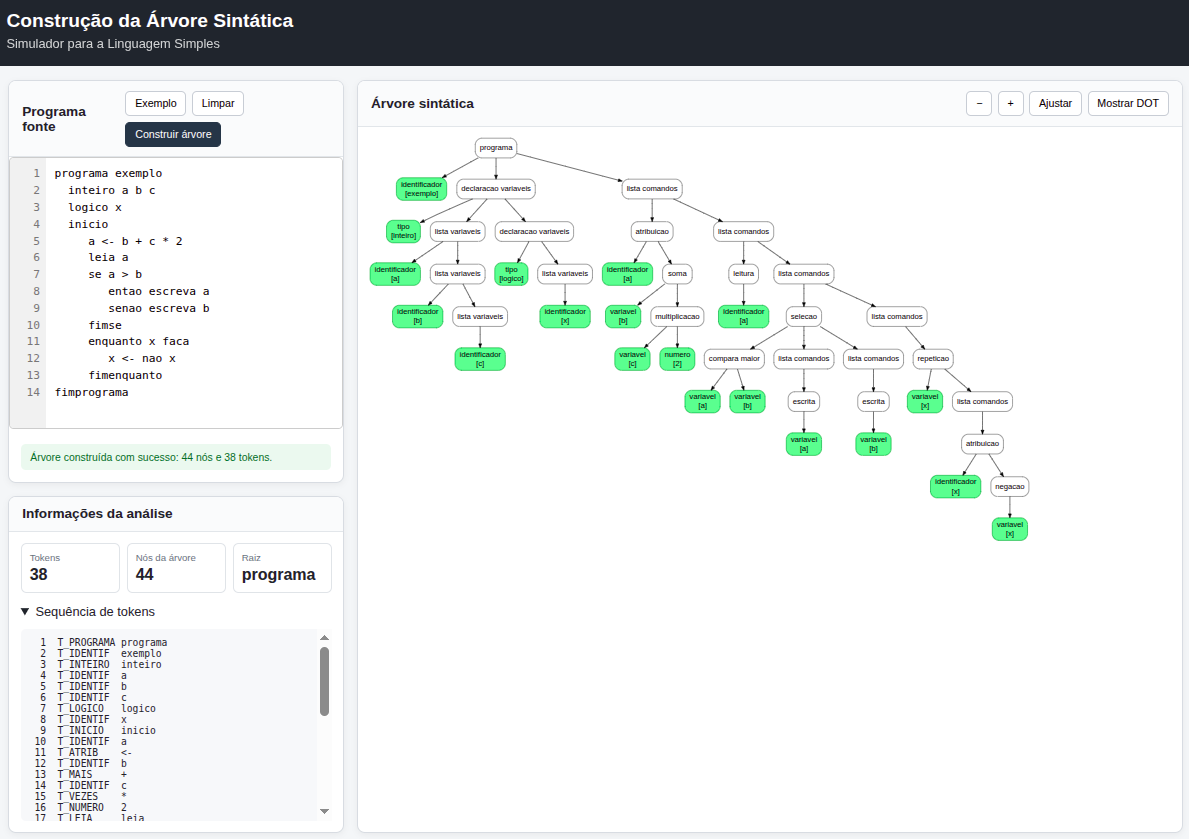
\includegraphics[width=0.6\textwidth]{chapters/images/printscreen/syntaxTree.png}}
\caption{Visualização da aplicação interativa}
\end{figure}
\begin{tcolorbox}[enhanced jigsaw, title=Acesso Interativo]
Acesse a simulação em:\par\smallskip
\small\url{https://luizedsilva.github.io/Livro-LTC/p5js/syntaxTree/}
\begin{center}
\includegraphics[width=3cm]{chapters/images/qrcode/syntaxTree.png}\end{center}
\end{tcolorbox}

Para obter mais informações sobre a biblioteca, consulte a documentação
oficial da \href{https://p5js.org/}{p5.js}.

Além dos exemplos interativos, os diagramas e ilustrações utilizados ao
longo do livro foram elaborados com ferramentas apropriadas para a
representação de estruturas formais e algoritmos. Entre elas encontra-se
o \textbf{Excalidraw}, utilizado na elaboração de diagramas e
ilustrações didáticas. Mais informações sobre a ferramenta podem ser
encontradas em \url{https://excalidraw.com}.

A produção deste livro teve como ponto de partida materiais didáticos,
exemplos e apresentações utilizados pelo autor na disciplina de
\textbf{Teoria de Linguagens e Compiladores}. Esses materiais foram
posteriormente reorganizados, ampliados e adaptados para constituir uma
obra estruturada em capítulos, com o objetivo de proporcionar uma
sequência de estudos mais adequada ao formato de livro.

A elaboração e a revisão do material contaram também com o auxílio de
ferramentas de \textbf{Inteligência Artificial}, utilizadas como apoio à
organização, revisão e aprimoramento de textos, exemplos e códigos. Todo
o conteúdo foi revisado, adaptado e validado pelo autor, que é
responsável pelo conteúdo apresentado e pelas decisões relativas à sua
organização e abordagem didática.

O livro foi produzido utilizando o \textbf{Quarto}, uma ferramenta de
publicação científica e técnica que permite gerar documentos e livros em
diferentes formatos a partir de arquivos de texto estruturados. A versão
em formato de livro foi construída utilizando o \textbf{Quarto Book}.
Para conhecer mais sobre essa ferramenta e suas possibilidades de
publicação, consulte \url{https://quarto.org/docs/books}.

Para um estudo mais aprofundado dos temas apresentados, recomenda-se a
consulta às obras clássicas e especializadas da área de linguagens
formais, teoria da computação, análise sintática e construção de
compiladores. Essas referências apresentam os fundamentos matemáticos e
os algoritmos discutidos neste livro com diferentes níveis de formalismo
e abrangência e constituem importantes fontes para o aprofundamento dos
estudos.

Espera-se que este livro possa servir como um primeiro contato
sistemático com a Teoria de Linguagens e a Construção de Compiladores,
oferecendo ao leitor não apenas os fundamentos teóricos necessários, mas
também oportunidades para experimentar, implementar e visualizar os
conceitos estudados. A combinação entre teoria, algoritmos, exemplos e
ferramentas interativas pretende tornar o estudo da área mais concreto e
favorecer a compreensão dos mecanismos que estão por trás do
processamento das linguagens de programação.

\pandocbounded{
\includegraphics[keepaspectratio]{cc-by-sa.png}}

Este trabalho está licenciado sob a Licença Creative Commons CC BY-SA
4.0.

\bookmarksetup{startatroot}

\chapter{Introdução à Teoria de
Linguagens}\label{introduuxe7uxe3o-uxe0-teoria-de-linguagens}

\begin{center}
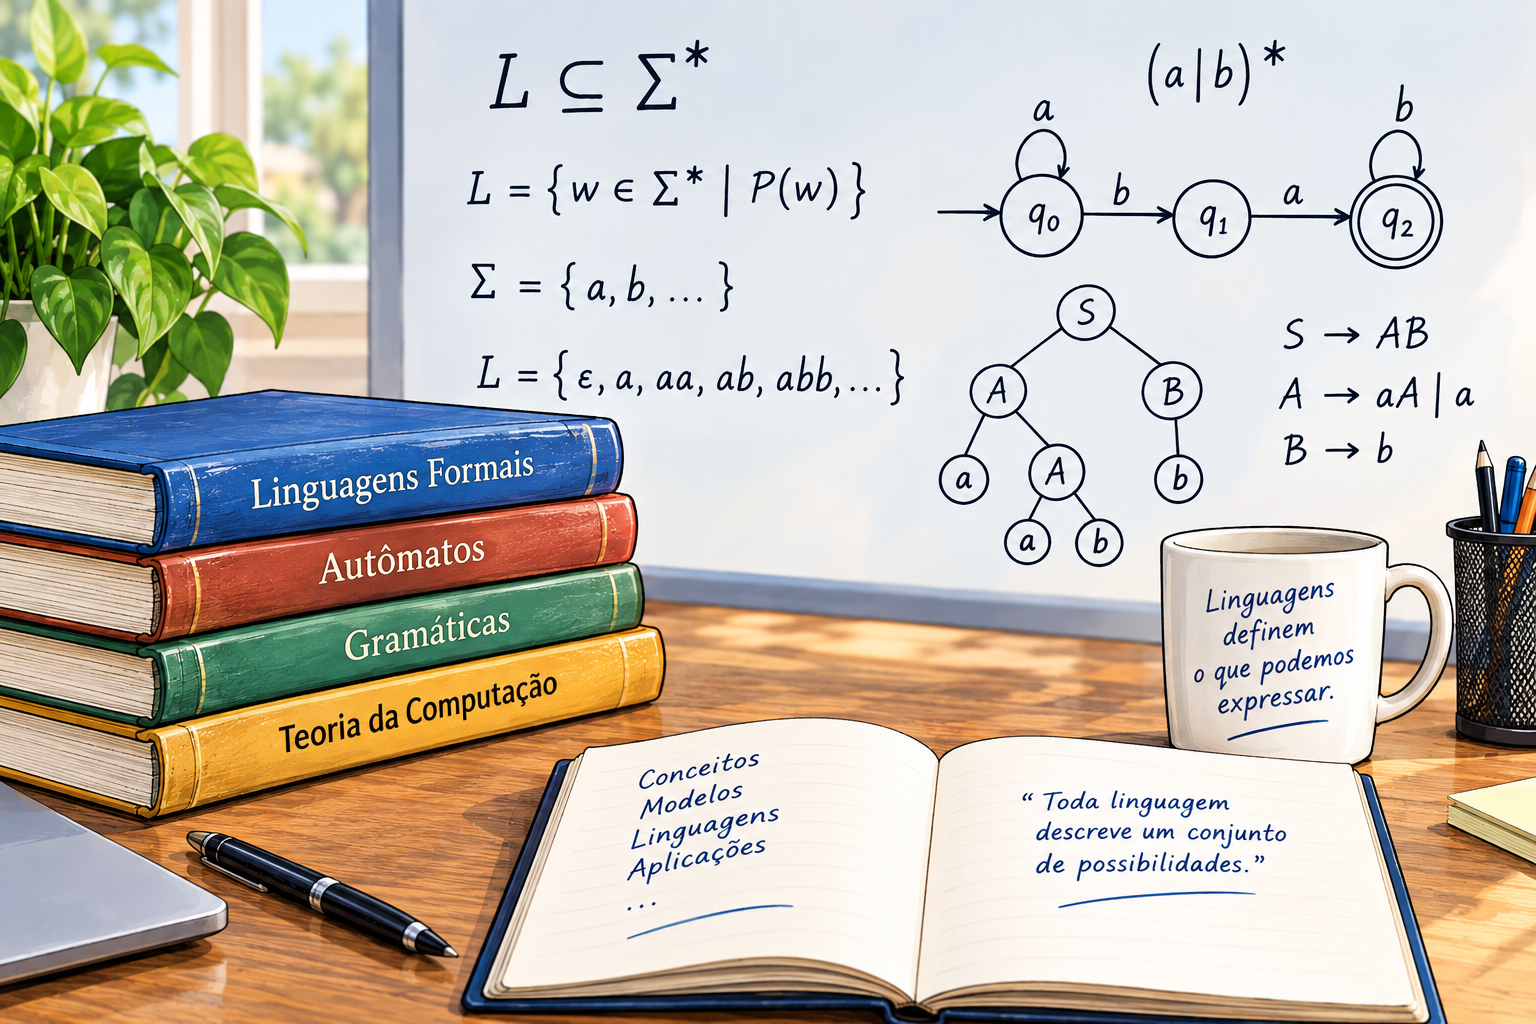
\includegraphics[width=0.7\linewidth,height=\textheight,keepaspectratio]{chapters/images/introducao.png}
\end{center}

\section{Computabilidade, Complexidade e
Autômatos}\label{computabilidade-complexidade-e-autuxf4matos}

A teoria da computação busca compreender os limites e as possibilidades
dos processos computacionais. Depois de estudar linguagens formais,
autômatos e técnicas de análise de linguagens, é natural avançar para
questões mais amplas: quais problemas podem ser resolvidos por um
computador?, quais problemas não podem ser resolvidos por nenhum
algoritmo? e quais recursos são necessários para resolver um problema
computável?. Essas questões conduzem aos conceitos de computabilidade e
complexidade computacional.

Além de determinar se um problema pode ser resolvido, a teoria da
complexidade procura determinar quais recursos computacionais são
necessários para resolvê-lo. Serão introduzidas as medidas de tempo e
espaço utilizadas para analisar algoritmos e as principais classes de
complexidade, permitindo distinguir problemas computáveis que podem ser
resolvidos de maneira eficiente daqueles para os quais não se conhecem
soluções eficientes.

Neste livro, serão apresentados ainda diferentes modelos formais de
computação e suas relações com os problemas que podem ser solucionados
algoritmicamente. Entre esses modelos estão os autômatos finitos, os
autômatos de pilha e as máquinas de Turing, que se diferenciam, entre
outros aspectos, pelos recursos de memória disponíveis e pelo poder
computacional que possuem. O estudo desses modelos permite compreender
como o poder computacional aumenta à medida que são incorporados novos
recursos de memória, estabelecendo uma relação entre linguagens e
modelos de computação.

A partir das máquinas de Turing, será possível estabelecer um modelo
geral de computação e investigar de forma mais abrangente a noção de
algoritmo, incluindo problemas para os quais não existe um procedimento
computacional capaz de produzir uma resposta para todas as entradas.
Nesse contexto, serão discutidos conceitos fundamentais como
decidibilidade, reconhecimento de linguagens e problemas indecidíveis.
Essa perspectiva permite estabelecer uma visão integrada da Teoria da
Computação, relacionando linguagens, autômatos, computabilidade e
complexidade, e mostrando como esses conceitos contribuem para os
fundamentos da Ciência da Computação.

Os conceitos de Computabilidade, complexidade e autômatos estão
relacionados ao \textbf{projeto e à implementação de compiladores}, pois
permitem compreender os limites teóricos e os recursos necessários para
processar linguagens de programação. Conforme será destacado no
desenvolvimento deste livro, os autômatos fornecem os modelos formais
utilizados nas diferentes etapas da análise de um programa: os
\textbf{autômatos finitos} fundamentam a análise léxica, enquanto os
\textbf{autômatos de pilha} e as gramáticas livres de contexto sustentam
a análise sintática. A teoria da computabilidade, por sua vez, permite
compreender quais problemas podem ou não ser resolvidos
algoritmicamente, estabelecendo limites para as tarefas que um
compilador pode realizar. Já a teoria da complexidade contribui para
avaliar o custo computacional dos algoritmos empregados no processo de
compilação, especialmente quando se busca desenvolver analisadores e
transformações eficientes. Dessa forma, autômatos, computabilidade e
complexidade constituem fundamentos teóricos que ajudam a explicar não
apenas \textbf{como} um compilador processa programas, mas também
\textbf{o que é possível processar e a que custo computacional}.

\subsection{Teoria da Complexidade}\label{teoria-da-complexidade}

A \textbf{Teoria da Complexidade Computacional} é um ramo da Ciência da
Computação que estuda a quantidade de recursos necessários para resolver
problemas computacionais. Entre esses recursos, destacam-se
principalmente o \textbf{tempo de execução}, correspondente ao número de
operações realizadas por um algoritmo, e o \textbf{espaço de memória},
correspondente à quantidade de memória utilizada durante sua execução. O
principal objetivo dessa área é compreender como esses recursos crescem
à medida que o tamanho da entrada aumenta, permitindo comparar
diferentes algoritmos e identificar aqueles mais adequados para resolver
um determinado problema.

Nem todos os problemas apresentam o mesmo grau de dificuldade
computacional. Alguns podem ser resolvidos de forma bastante eficiente,
mesmo quando a quantidade de dados é muito grande. Outros, entretanto,
tornam-se rapidamente inviáveis à medida que o tamanho da entrada
cresce. Um exemplo clássico de problema relativamente simples é a
ordenação de um vetor de números. Existem diversos algoritmos capazes de
ordenar milhões de elementos em poucos segundos, tornando essa tarefa
perfeitamente viável na prática. Em contraste, problemas como a
elaboração automática do horário de aulas de uma universidade envolvem
inúmeras restrições e combinações possíveis. É necessário considerar
disponibilidade de professores, salas, disciplinas, turmas e conflitos
de horários, fazendo com que o número de soluções possíveis cresça
exponencialmente. Consequentemente, encontrar a melhor solução pode
exigir um esforço computacional extremamente elevado.

Para analisar esse comportamento, a Teoria da Complexidade utiliza a
\textbf{notação assintótica}, sendo a mais conhecida a \textbf{notação
Big-O}, representada por \(O(\cdot)\). Essa notação descreve como o
tempo de execução ou o consumo de memória de um algoritmo cresce em
função do tamanho da entrada, normalmente representado por \(n\). Por
exemplo, um algoritmo de complexidade \(O(1)\) executa sempre o mesmo
número de operações, independentemente da quantidade de dados.
Algoritmos com complexidade \(O(\log n)\), como a busca binária, crescem
muito lentamente e permanecem eficientes mesmo para entradas muito
grandes. Já algoritmos com complexidade \(O(n)\) apresentam crescimento
linear, enquanto algoritmos \(O(n^2)\), comuns em métodos simples de
ordenação, têm seu tempo de execução aumentando quadraticamente conforme
a entrada cresce.

À medida que surgem problemas mais difíceis, aparecem também novas
classes de complexidade, como \(O(2^n)\) e \(O(n!)\), cujo crescimento é
tão acelerado que inviabiliza sua resolução exata para entradas
relativamente pequenas. Esses problemas são frequentemente classificados
como \textbf{intratáveis}, pois, embora possuam solução teórica, o tempo
necessário para obtê-la pode ultrapassar a idade do universo mesmo
utilizando computadores extremamente rápidos. A identificação desses
limites é uma das principais contribuições da Teoria da Complexidade.

Quando um problema apresenta alta complexidade computacional, nem sempre
é possível encontrar uma solução ótima em tempo razoável. Nesses casos,
diversas estratégias podem ser empregadas. Uma possibilidade consiste em
simplificar o problema original, reduzindo o número de restrições ou
considerando apenas parte dos dados disponíveis. Outra alternativa é
utilizar \textbf{algoritmos aproximativos}, que produzem soluções
próximas da ideal, mas em um tempo significativamente menor. Também são
amplamente empregadas técnicas probabilísticas e heurísticas, como
algoritmos genéticos, colônia de formigas, recozimento simulado
(\emph{simulated annealing}), busca tabu e métodos de otimização
baseados em inteligência artificial. Embora essas técnicas não garantam
a obtenção da melhor solução possível, frequentemente produzem
resultados de excelente qualidade em aplicações reais.

A Teoria da Complexidade possui aplicações em praticamente todas as
áreas da computação, incluindo otimização, inteligência artificial,
pesquisa operacional, bioinformática, logística e redes de computadores.
Uma de suas aplicações mais importantes está na \textbf{criptografia
moderna}. Os principais sistemas criptográficos utilizados atualmente,
como RSA e criptografia baseada em curvas elípticas, fundamentam sua
segurança na dificuldade computacional de determinados problemas
matemáticos. A ideia central é que algumas operações, como multiplicar
dois números primos muito grandes, são realizadas rapidamente, enquanto
a operação inversa --- fatorar o produto obtido --- é extremamente
difícil do ponto de vista computacional. Dessa forma, a segurança das
comunicações digitais depende justamente da existência de problemas para
os quais não se conhecem algoritmos eficientes de solução. Assim,
compreender a complexidade dos problemas não apenas permite desenvolver
algoritmos mais rápidos, mas também é essencial para projetar sistemas
computacionais seguros e confiáveis.

\subsection{Teoria da Computabilidade}\label{teoria-da-computabilidade}

A Teoria da Computabilidade é o ramo da Ciência da Computação que estuda
os limites fundamentais da computação. Seu principal objetivo é
responder à seguinte pergunta: quais problemas podem ser resolvidos por
um algoritmo? Diferentemente da Teoria da Complexidade, que procura
medir o custo computacional necessário para resolver um problema, a
Teoria da Computabilidade investiga se uma solução algorítmica existe.
Em outras palavras, essa área busca determinar se é possível construir
um procedimento mecânico que, para qualquer entrada válida, produza a
resposta correta em um número finito de passos.

No final do século XIX, a matemática atravessava um período de intensa
expansão, mas também de profundas incertezas. Novas teorias surgiam
rapidamente, enquanto paradoxos relacionados à Teoria dos Conjuntos
colocavam em dúvida a consistência dos fundamentos matemáticos. Nesse
contexto, o matemático alemão \textbf{David Hilbert (1862--1943)} propôs
um ambicioso programa de pesquisa, conhecido como \textbf{Programa de
Hilbert}, cujo objetivo era estabelecer uma base sólida para toda a
matemática.

A proposta de Hilbert consistia em \textbf{formalizar completamente a
matemática}, reescrevendo todas as demonstrações por meio de um sistema
finito de axiomas e regras de inferência rigorosamente definidas. Em
outras palavras, qualquer demonstração matemática deveria poder ser
realizada como uma sequência mecânica de aplicações de regras lógicas,
eliminando ambiguidades e garantindo que toda conclusão fosse obtida de
forma objetiva. Hilbert também desejava demonstrar que esse sistema
seria \textbf{consistente} (livre de contradições), \textbf{completo}
(capaz de provar toda afirmação verdadeira expressável no sistema) e
\textbf{decidível}, isto é, deveria existir um procedimento mecânico
capaz de determinar, em tempo finito, se qualquer proposição matemática
é verdadeira ou falsa.

Em 1900, durante o Congresso Internacional de Matemáticos realizado em
Paris, Hilbert apresentou uma lista de \textbf{23 problemas} que
considerava fundamentais para o desenvolvimento da matemática no século
XX. Esses problemas orientaram décadas de pesquisa em diversas áreas e
muitos deles permanecem influentes até os dias atuais. Posteriormente,
foir proposto o chamado \textbf{Entscheidungsproblem} (problema da
decisão), formulado de maneira mais explícita por David Hilbert e
Wilhelm Ackermann na década de 1920. O problema consistia em responder à
seguinte pergunta: \textbf{existe um procedimento geral que possa
decidir automaticamente se qualquer afirmação matemática é
demonstrável?}

Responder a essa questão exigia, antes de tudo, definir com precisão o
que significa um \textbf{procedimento mecânico} ou um
\textbf{algoritmo}. Até então, essa ideia era intuitiva, mas não possuía
uma definição matemática rigorosa. Em 1936, o matemático britânico
\textbf{Alan Turing} apresentou uma resposta inovadora ao introduzir um
modelo abstrato de computação, hoje conhecido como \textbf{Máquina de
Turing}. Esse modelo descreve uma máquina extremamente simples, capaz de
ler, escrever e modificar símbolos em uma fita infinita seguindo um
conjunto finito de regras. Apesar de sua simplicidade, Turing demonstrou
que esse modelo é capaz de representar qualquer algoritmo executável.

Utilizando esse modelo, Turing provou que \textbf{não existe um
algoritmo capaz de decidir, para toda proposição matemática, se ela é
demonstrável}. Para isso, demonstrou inicialmente a inexistência de um
algoritmo geral para resolver o chamado \textbf{Problema da Parada
(Halting Problem)}, isto é, determinar se um programa qualquer terminará
sua execução ou permanecerá executando indefinidamente. A partir desse
resultado, concluiu-se que o \emph{Entscheidungsproblem} possui resposta
negativa: existem problemas matemáticos que nenhum procedimento mecânico
pode resolver.

Esse trabalho marcou o nascimento da \textbf{Teoria da Computabilidade}
e estabeleceu as bases da Ciência da Computação moderna. A Máquina de
Turing tornou-se o principal modelo teórico para o estudo dos
algoritmos, dos limites da computação e da classificação dos problemas
em \textbf{computáveis} e \textbf{não computáveis}. Além disso, suas
ideias influenciaram profundamente o desenvolvimento das linguagens de
programação, dos compiladores e da própria arquitetura dos computadores
digitais.

\subsection{Teoria dos Autômatos}\label{teoria-dos-autuxf4matos}

A \textbf{Teoria dos Autômatos} é o ramo da Ciência da Computação que
estuda modelos matemáticos capazes de representar máquinas abstratas de
processamento de informações, denominadas \textbf{autômatos}. Esses
modelos descrevem, de maneira formal, como um sistema recebe uma
sequência de símbolos como entrada, altera seu estado interno de acordo
com regras previamente definidas e produz uma resposta, que normalmente
consiste em aceitar ou rejeitar a entrada. Embora sejam construções
puramente matemáticas, os autômatos constituem uma das bases teóricas da
computação moderna e permitem compreender o funcionamento de diversos
sistemas computacionais.

O conceito de autômato surgiu da necessidade de representar algoritmos
de forma abstrata, sem depender das características específicas de um
computador físico. Dessa forma, é possível estudar as propriedades dos
algoritmos, das linguagens e dos problemas computacionais utilizando
modelos simples e rigorosamente definidos. Cada tipo de autômato possui
capacidades computacionais próprias e é capaz de reconhecer determinadas
classes de linguagens formais, estabelecendo uma estreita relação entre
a Teoria dos Autômatos e a Teoria das Linguagens Formais.

O modelo mais simples é o \textbf{autômato finito}, cuja principal
característica é possuir um número limitado de estados e não dispor de
memória além do estado atual. Apesar dessa simplicidade, os autômatos
finitos possuem inúmeras aplicações práticas. Eles são utilizados em
ferramentas de busca de padrões em textos, reconhecimento de palavras,
validação de entradas em formulários, protocolos de comunicação,
circuitos digitais e sistemas de controle. Uma das aplicações mais
importantes encontra-se na construção de compiladores, onde autômatos
finitos são empregados na \textbf{análise léxica}, responsável por
identificar palavras reservadas, identificadores, números, operadores e
demais símbolos que compõem um programa.

Para reconhecer linguagens mais complexas, que apresentam estruturas
aninhadas ou dependências hierárquicas, é necessário utilizar modelos
computacionais mais poderosos. Os \textbf{autômatos de pilha} estendem
os autômatos finitos por meio da adição de uma estrutura de memória
denominada \textbf{pilha}, que permite armazenar informações temporárias
durante o processamento da entrada. Graças a essa memória adicional,
esses autômatos conseguem reconhecer as \textbf{linguagens livres de
contexto}, fundamentais para a descrição da sintaxe das linguagens de
programação. Em consequência, os autômatos de pilha são amplamente
utilizados na implementação da \textbf{análise sintática} de
compiladores e interpretadores, verificando se um programa está de
acordo com as regras gramaticais da linguagem.

Além das aplicações em compiladores, modelos baseados em autômatos
aparecem em diversas áreas da computação. Na inteligência artificial,
por exemplo, máquinas de estados são empregadas para modelar o
comportamento de agentes inteligentes, personagens de jogos digitais e
robôs autônomos. Em engenharia de software, diagramas de estados são
utilizados para especificar o comportamento de sistemas reativos e
protocolos de comunicação. Em redes de computadores, autômatos
representam o funcionamento de protocolos de transmissão de dados,
enquanto na bioinformática são utilizados para análise de sequências de
DNA e proteínas. Essas aplicações demonstram que os autômatos constituem
uma ferramenta versátil para representar sistemas que evoluem entre
diferentes estados de acordo com eventos ou entradas recebidas.

A Teoria dos Autômatos também estabelece uma importante hierarquia entre
diferentes modelos de computação. À medida que novos recursos de memória
são adicionados aos autômatos, sua capacidade computacional aumenta.
Assim, autômatos finitos reconhecem linguagens regulares; autômatos de
pilha reconhecem linguagens livres de contexto; máquinas de Turing, por
sua vez, representam o modelo computacional mais geral conhecido e são
capazes de executar qualquer algoritmo computável. Essa relação entre
modelos computacionais e classes de linguagens é formalizada pela
\textbf{Hierarquia de Chomsky}, um dos pilares da Teoria das Linguagens
Formais.

Além de suas aplicações práticas, a Teoria dos Autômatos fornece o
\textbf{formalismo matemático} utilizado pelas teorias da
Computabilidade e da Complexidade. A definição rigorosa de modelos
computacionais permite estabelecer quais problemas podem ser resolvidos
por algoritmos, quais estão além dos limites da computação e quanto
tempo ou memória são necessários para resolver determinados problemas.
Em outras palavras, antes de estudar a eficiência de um algoritmo ou os
limites da computação, é necessário definir formalmente o que significa
``computar'', e essa definição é fornecida pelos modelos estudados na
Teoria dos Autômatos.

Ao longo deste livro, os diferentes modelos de autômatos serão
apresentados de forma progressiva, iniciando pelos autômatos finitos,
passando pelos autômatos de pilha e culminando nas máquinas de Turing.
Esse percurso permitirá compreender não apenas como esses modelos
funcionam, mas também como eles se relacionam com as linguagens formais,
os compiladores e os fundamentos teóricos da Ciência da Computação.
Dessa maneira, a Teoria dos Autômatos serve como elo entre os conceitos
matemáticos abstratos e as aplicações práticas que sustentam o
desenvolvimento de linguagens de programação, compiladores e diversos
sistemas computacionais utilizados atualmente.

\bookmarksetup{startatroot}

\chapter{Introdução aos
Compiladores}\label{introduuxe7uxe3o-aos-compiladores}

\begin{center}
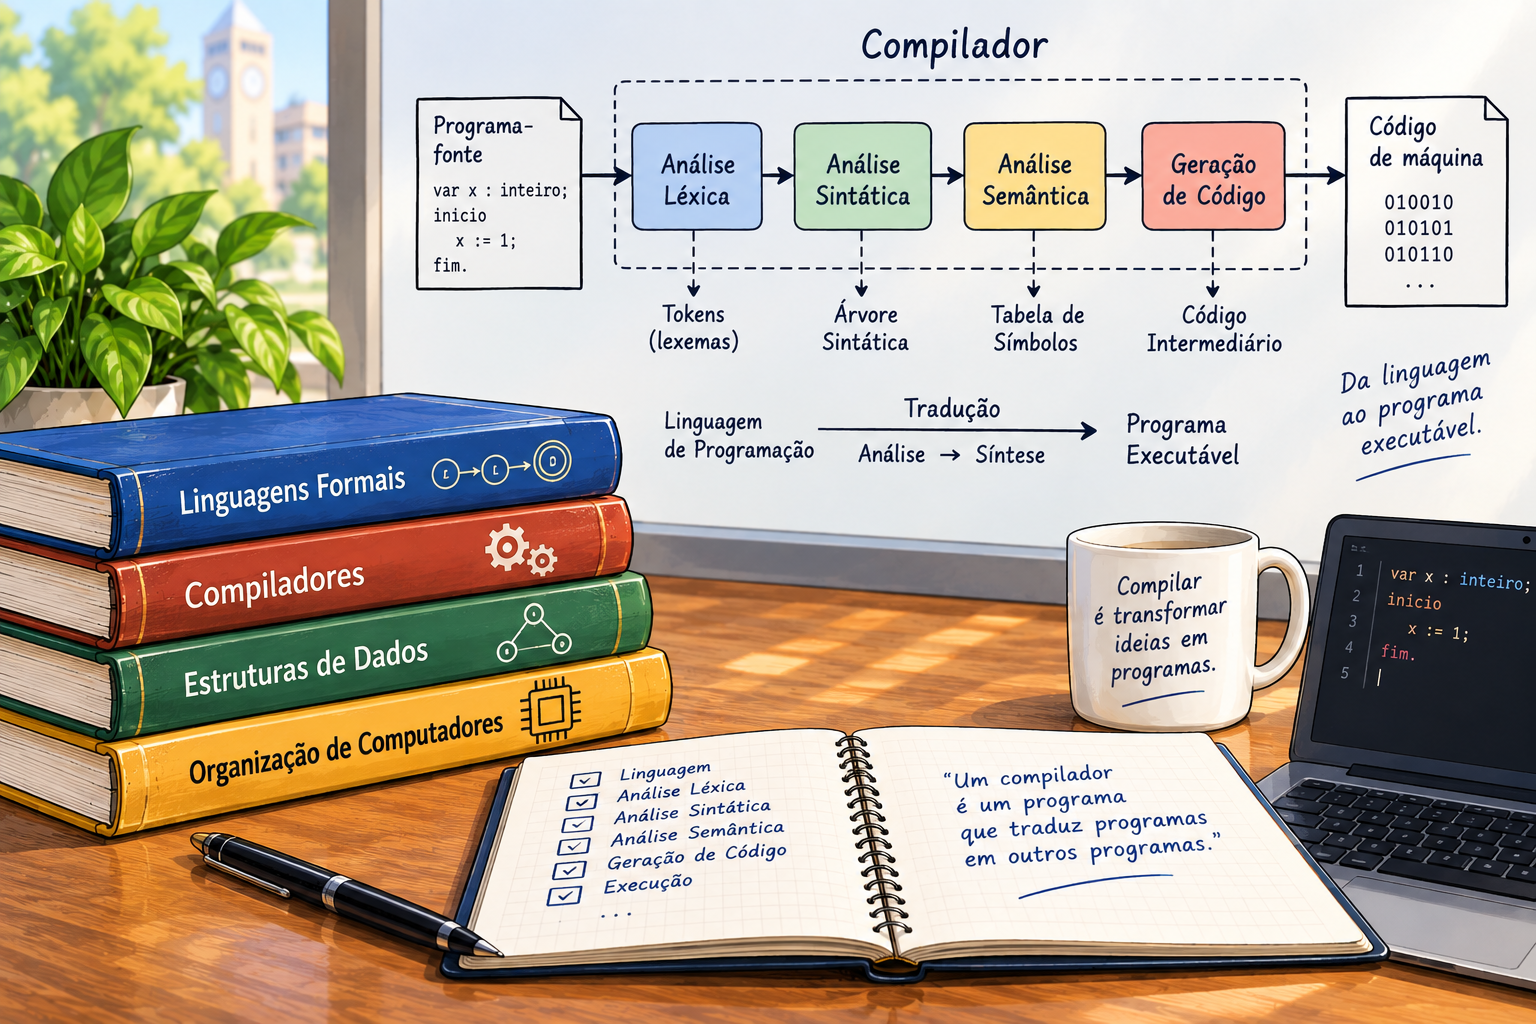
\includegraphics[width=0.7\linewidth,height=\textheight,keepaspectratio]{chapters/images/compilador.png}
\end{center}

\section{Introdução}\label{introduuxe7uxe3o}

Desde o surgimento dos computadores digitais, existe uma preocupação
fundamental: como permitir que seres humanos expressem instruções de
maneira conveniente e, ao mesmo tempo, como transformar essas instruções
em uma forma que possa ser processada por uma máquina? Os computadores
são capazes de executar operações em grande velocidade, mas precisam
receber instruções em uma representação que possa ser interpretada pelos
seus componentes de processamento. A necessidade de estabelecer uma
ponte entre a forma de expressão utilizada pelas pessoas e a
representação utilizada pelos computadores levou ao desenvolvimento das
\textbf{linguagens de programação} e dos sistemas responsáveis por
processá-las.

Os primeiros programas eram escritos utilizando diretamente as
instruções disponíveis no processador. Essas instruções são
representadas por códigos binários ou, em uma forma mais legível, por
\textbf{linguagens de montagem}, conhecidas como \emph{assembly
languages}. Em uma linguagem de montagem, as instruções são
representadas por mnemônicos que correspondem, de maneira relativamente
direta, às instruções da arquitetura do processador. Embora representem
uma evolução em relação à programação diretamente em código de máquina,
as linguagens de montagem ainda mantêm uma forte dependência da
arquitetura do computador. \cite{aho,ziviani,price,louden,tomasz}

A necessidade de aumentar a produtividade dos programadores e reduzir a
dependência em relação ao hardware levou ao desenvolvimento das
\textbf{linguagens de programação de alto nível}. Na década de 1950
surgiram linguagens como FORTRAN e, posteriormente, ALGOL 60. Essas
linguagens permitiram que algoritmos fossem descritos de maneira mais
próxima da forma utilizada para expressar problemas matemáticos e
procedimentos, reduzindo a quantidade de detalhes relacionados
diretamente ao funcionamento do processador.

Desde então, centenas de linguagens de programação foram desenvolvidas.
Algumas foram projetadas para aplicações científicas e numéricas;
outras, para sistemas operacionais, inteligência artificial,
processamento de dados, desenvolvimento Web, sistemas embarcados ou
computação de alto desempenho. Apesar das diferenças entre elas, todas
precisam, de alguma maneira, ter suas instruções transformadas em uma
representação que possa ser executada ou processada por um computador.

Essa necessidade deu origem aos \textbf{programas tradutores}. Um
tradutor é um programa capaz de receber uma representação de um programa
e produzir outra representação equivalente, normalmente preservando o
significado computacional do programa original.

De maneira geral, podemos representar esse processo na
Figura~\ref{fig-compiler-process}.

\begin{figure}

\centering{

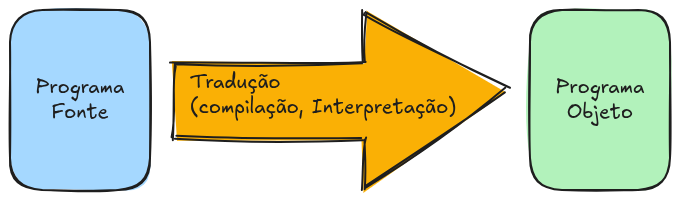
\includegraphics[width=0.6\linewidth,height=\textheight,keepaspectratio]{chapters/images/compiler-process.png}

}

\caption{\label{fig-compiler-process}Processo de
compilação/interpretação}

\end{figure}%

O programa recebido pelo tradutor é denominado \textbf{programa-fonte}
(\emph{source program}) e a representação produzida é denominada
\textbf{programa-alvo} (\emph{target program}) ou, em determinados
contextos, \textbf{programa-objeto} (\emph{object program}).

O programa-fonte é escrito em uma linguagem de programação, como C, C++,
Java, Rust ou outra linguagem de alto nível. O programa-alvo pode ser
código de máquina, código objeto, código intermediário, \emph{bytecode}
ou alguma outra representação adequada ao sistema que realizará a
execução.

O desenvolvimento de um programa, portanto, envolve mais do que
simplesmente escrever uma sequência de instruções. É necessário que
exista um mecanismo capaz de analisar o programa escrito pelo
programador, verificar se sua estrutura está de acordo com as regras da
linguagem e produzir uma representação que possa ser utilizada
posteriormente para execução.

\subsection{Compiladores}\label{compiladores}

Um \textbf{compilador} é um programa tradutor que recebe um programa
escrito em uma linguagem-fonte e produz uma representação em uma
linguagem-alvo.

Um exemplo tradicional é um compilador que recebe um programa escrito em
C e produz código objeto ou código de máquina para uma determinada
arquitetura.

O compilador não precisa necessariamente produzir diretamente código de
máquina. Em muitos sistemas, o resultado da compilação é uma
representação intermediária que será posteriormente transformada em
código de máquina ou executada por uma máquina virtual.

O processo de compilação normalmente envolve diversas etapas. Entre elas
estão a análise dos caracteres que formam o programa, a identificação
dos elementos da linguagem, a análise da estrutura sintática, a
verificação de propriedades semânticas, a geração de uma representação
intermediária e a geração ou otimização do código-alvo.

Essas etapas não são necessariamente implementadas como programas
independentes. Um compilador pode organizá-las de diferentes maneiras e
várias etapas podem ser combinadas em uma mesma passagem pelo programa.

\subsection{Interpretadores}\label{interpretadores}

Outra forma de executar programas escritos em linguagens de alto nível é
utilizar um \textbf{interpretador}.

Um interpretador recebe um programa-fonte e executa suas instruções por
meio de um processo de análise e execução.

Enquanto em uma compilação tradicional o programa-fonte é traduzido para
uma representação-alvo antes de sua execução, em uma interpretação o
processamento do programa está diretamente associado à sua execução.

É comum utilizar os termos \textbf{tradução offline} e \textbf{tradução
online} para estabelecer uma distinção didática entre essas abordagens.
Na tradução offline, o programa é processado antes da execução, e o
resultado da tradução pode ser armazenado para ser executado
posteriormente. Na interpretação, o processamento necessário para
executar o programa ocorre durante a execução.

Essa distinção, entretanto, deve ser entendida como uma simplificação.
Sistemas modernos frequentemente combinam técnicas de compilação e
interpretação. Uma linguagem pode, por exemplo, ser inicialmente
traduzida para um código intermediário e posteriormente interpretada ou
compilada dinamicamente para código de máquina.

\subsection{Compilação e
interpretação}\label{compilauxe7uxe3o-e-interpretauxe7uxe3o}

As diferenças entre compilação e interpretação podem ser observadas a
partir do momento em que ocorre a transformação do programa.

Em uma compilação tradicional, temos uma sequência semelhante a

\[
\text{Fonte}
\xrightarrow{\text{compilação}}
\text{Alvo}
\xrightarrow{\text{execução}}
\text{Resultado}.
\]

O programa-alvo pode ser armazenado e executado posteriormente sem que
seja necessário repetir todo o processo de compilação.

Em uma interpretação, podemos representar o processo como

\[
\text{Fonte}
\xrightarrow{\text{interpretação}}
\text{Execução}.
\]

O interpretador participa diretamente do processo de execução.

Na prática, essas duas estratégias não são mutuamente exclusivas.
Máquinas virtuais, linguagens com código intermediário e compiladores
\emph{Just-In-Time} (JIT) utilizam combinações dessas técnicas. Dessa
forma, a fronteira entre compilação e interpretação em sistemas modernos
é menos rígida do que a representação tradicional pode sugerir.

O ponto fundamental é que programas escritos em linguagens de alto nível
precisam ser processados por algum mecanismo capaz de transformar suas
construções em operações que possam ser efetivamente executadas.

\subsection{O programa-fonte}\label{o-programa-fonte}

Um programa-fonte é uma sequência de caracteres que segue as regras de
uma determinada linguagem de programação. Por exemplo, considere o
seguinte programa em uma linguagem semelhante a C:

\begin{Shaded}
\begin{Highlighting}[]
\DataTypeTok{int}\NormalTok{ soma}\OperatorTok{(}\DataTypeTok{int}\NormalTok{ a}\OperatorTok{,} \DataTypeTok{int}\NormalTok{ b}\OperatorTok{)} \OperatorTok{\{}
    \ControlFlowTok{return}\NormalTok{ a }\OperatorTok{+}\NormalTok{ b}\OperatorTok{;}
\OperatorTok{\}}
\end{Highlighting}
\end{Shaded}

Para um programador, esse código apresenta uma estrutura relativamente
fácil de compreender. Entretanto, antes que possa ser executado por um
processador, é necessário determinar o significado dos elementos que
aparecem no programa e transformá-los em uma representação adequada.

O compilador precisa identificar, entre outras coisas, os
identificadores \texttt{soma}, \texttt{a} e \texttt{b}, as palavras
reservadas \texttt{int} e \texttt{return}, os símbolos \texttt{(},
\texttt{)}, \texttt{\{}, \texttt{\}}, \texttt{,} e \texttt{;}, além do
operador \texttt{+}.

Também é necessário verificar se esses elementos estão organizados de
acordo com a sintaxe da linguagem e se o programa satisfaz determinadas
regras semânticas. Somente depois dessas análises será possível produzir
uma representação adequada para as etapas seguintes da compilação.

Esse exemplo simples já evidencia uma característica fundamental dos
compiladores: \textbf{o programa-fonte precisa ser analisado em
diferentes níveis}.

\section{Aspectos básicos da
compilação}\label{aspectos-buxe1sicos-da-compilauxe7uxe3o}

A implementação de uma linguagem de programação envolve diferentes
questões relacionadas à forma como os programas são escritos, analisados
e transformados para que possam ser executados por um computador. De
maneira geral, podem ser identificados três aspectos fundamentais: o
aspecto sintático, o aspecto semântico e o aspecto pragmático.

O \textbf{aspecto sintático} está relacionado à forma das construções da
linguagem. Seu objetivo é determinar se uma determinada sequência de
símbolos constitui uma construção válida segundo as regras da linguagem.
Assim, a análise sintática permite verificar, por exemplo, se uma
expressão, uma atribuição, uma declaração ou um comando de repetição foi
escrito de acordo com a gramática da linguagem.

O \textbf{aspecto semântico} está relacionado ao significado das
construções sintaticamente válidas. Uma construção pode estar
corretamente formada de acordo com a gramática e, ainda assim, não
possuir um significado válido no contexto do programa. São exemplos de
problemas semânticos a utilização de uma variável que não foi declarada,
a incompatibilidade entre tipos em uma atribuição e a utilização
inadequada de uma operação em função dos tipos de seus operandos.

O \textbf{aspecto pragmático} está relacionado à integração do processo
de tradução com o sistema computacional no qual o programa será
executado. Esse aspecto envolve características da máquina hospedeira e
da máquina-alvo, do sistema operacional, do formato dos arquivos
executáveis, das convenções de chamada de procedimentos e funções, da
organização da memória e do conjunto de instruções do processador.

Os aspectos sintático e semântico podem ser estudados de maneira
relativamente independente da arquitetura específica do computador. Já
os aspectos relacionados à geração e à execução do código apresentam
maior dependência da plataforma-alvo. Uma mesma linguagem de programação
pode, por exemplo, ser implementada para diferentes arquiteturas,
exigindo estratégias distintas para a geração do código executável.

Por essa razão, o estudo dos compiladores pode ser realizado com o
auxílio de uma linguagem de programação simplificada. Neste livro, os
exemplos serão desenvolvidos com base em uma linguagem denominada
\textbf{Linguagem Simples}, cuja tradução será direcionada para uma
máquina virtual também simplificada, denominada \textbf{Máquina Virtual
Simples (MVS)}. Nessa abordagem, os aspectos pragmáticos da linguagem e
os detalhes da arquitetura da máquina são deliberadamente reduzidos.
Essa simplificação permite concentrar a atenção nos princípios e nas
técnicas fundamentais envolvidos na construção de compiladores, sem
introduzir, inicialmente, a complexidade característica das linguagens
de programação de grande porte e os diversos detalhes presentes em
arquiteturas reais de computadores.

\section{Fases da compilação}\label{fases-da-compilauxe7uxe3o}

O processo de compilação pode ser organizado em um conjunto de fases,
cada uma responsável por uma parte específica da transformação do
programa fonte. Uma organização tradicional compreende as fases de
análise léxica, análise sintática, análise semântica, geração de código
intermediário, otimização e geração de código para a máquina-alvo.

A \textbf{análise léxica} é responsável por percorrer o programa fonte e
identificar as unidades básicas que o constituem, denominadas
\emph{tokens}. Nessa fase são reconhecidos, por exemplo,
identificadores, palavras reservadas, operadores, delimitadores e
constantes.

A \textbf{análise sintática} recebe os \emph{tokens} produzidos pelo
analisador léxico e verifica se eles podem ser organizados de acordo com
as regras gramaticais da linguagem. Como resultado dessa análise, pode
ser construída uma representação da estrutura sintática do programa,
frequentemente na forma de uma árvore sintática ou de uma árvore
sintática abstrata.

A \textbf{análise semântica} utiliza a estrutura produzida pela análise
sintática para verificar propriedades que não podem ser determinadas
apenas pela gramática. Entre essas propriedades encontram-se a
compatibilidade de tipos, a declaração e o uso de identificadores, as
regras de escopo e a consistência das operações realizadas pelo
programa.

Após as fases de análise, o compilador pode produzir uma
\textbf{representação intermediária} do programa. Essa representação
funciona como uma forma de código independente, ou relativamente
independente, da arquitetura da máquina-alvo. A utilização de uma
representação intermediária facilita a implementação de compiladores
para diferentes arquiteturas, pois permite separar as etapas de análise
das etapas específicas de geração de código.

A \textbf{otimização} procura transformar a representação do programa de
modo a obter uma implementação mais eficiente, preservando seu
comportamento. Dependendo da estratégia utilizada, a otimização pode
buscar reduzir o espaço ocupado pelo programa ou diminuir seu tempo de
execução.

Finalmente, a \textbf{geração de código} transforma a representação
intermediária em uma representação adequada à máquina ou
plataforma-alvo. O resultado pode ser código de máquina, código objeto,
código para uma máquina virtual ou outra representação apropriada ao
ambiente de execução.

A Figura~\ref{fig-fases} apresenta uma visão geral dessas fases.

\begin{figure}

\centering{

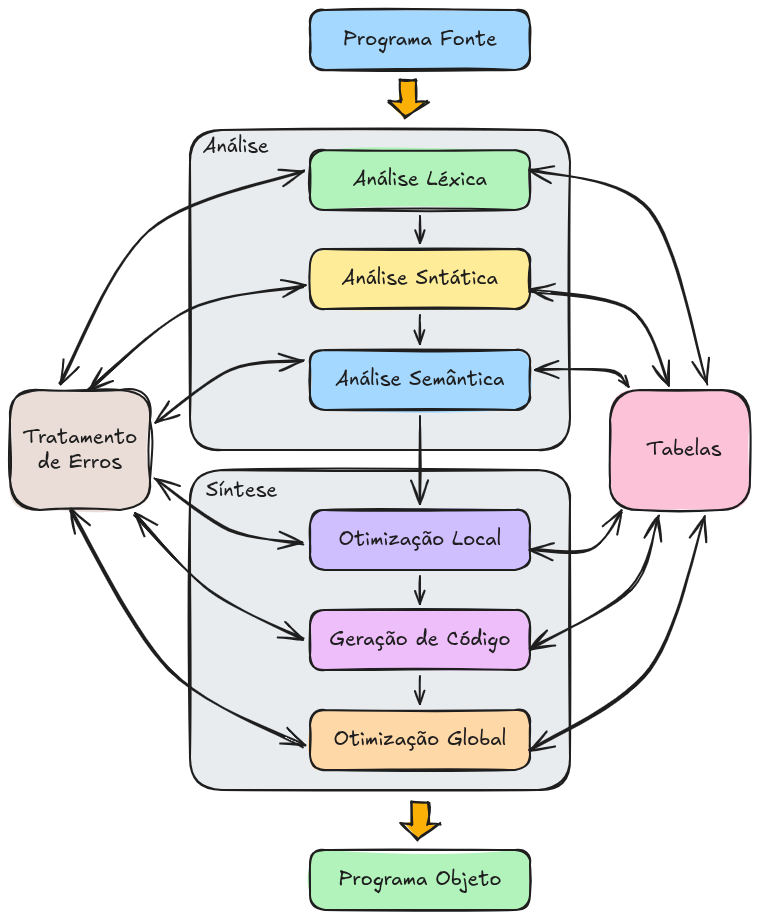
\includegraphics[width=0.7\linewidth,height=\textheight,keepaspectratio]{chapters/images/fases.png}

}

\caption{\label{fig-fases}As fases da compilação}

\end{figure}%

O processo apresentado na Figura~\ref{fig-fases} deve ser entendido como
uma organização conceitual. Em um compilador real, algumas dessas fases
podem ser combinadas, executadas mais de uma vez ou implementadas de
maneira integrada. Além disso, informações produzidas em uma determinada
fase podem ser utilizadas por diversas outras fases.

Durante o processo de análise, o compilador pode identificar diferentes
categorias de erros. Os \textbf{erros léxicos} estão relacionados a
símbolos ou sequências de caracteres que não pertencem ao vocabulário da
linguagem. Os \textbf{erros sintáticos} ocorrem quando os \emph{tokens}
não podem ser organizados segundo as regras da gramática. Já os
\textbf{erros semânticos} ocorrem quando uma construção sintaticamente
válida viola alguma regra de significado da linguagem.

As fases de compilação podem ser organizadas de diferentes maneiras. Em
uma \textbf{compilação em múltiplos passos}, cada fase pode produzir uma
representação intermediária que será utilizada pela fase seguinte. Essa
organização favorece a separação das responsabilidades e pode facilitar
a construção e a manutenção do compilador.

Em uma \textbf{compilação em uma única passagem}, por outro lado, as
diferentes atividades podem ser combinadas de modo que o programa seja
processado e traduzido de maneira mais integrada. Historicamente, essa
estratégia foi importante em ambientes nos quais os recursos
computacionais eram limitados. Atualmente, a distinção entre
compiladores de uma e de várias passagens é menos rígida, pois
compiladores modernos utilizam diferentes formas de organização interna
e múltiplas representações intermediárias.

Uma estratégia particularmente importante para a implementação de
compiladores é a \textbf{tradução dirigida pela sintaxe}. Nesse modelo,
as ações responsáveis pelo processamento semântico e pela geração de
código são associadas às regras da gramática utilizada pelo analisador
sintático. Assim, à medida que uma construção sintática é reconhecida,
podem ser executadas ações associadas àquela construção.

As ações semânticas podem, por exemplo, atualizar a tabela de símbolos,
realizar verificações de tipos, calcular atributos de uma construção ou
produzir instruções para uma representação intermediária. Dessa maneira,
a análise sintática passa a desempenhar um papel central na coordenação
das demais atividades de tradução.

No projeto de compilador desenvolvido neste curso, será utilizada essa
abordagem, com o auxílio das ferramentas \emph{flex} e \emph{bison}.
Essas ferramentas permitem automatizar parte significativa da construção
dos analisadores léxico e sintático, possibilitando concentrar o estudo
nos princípios envolvidos na implementação de um compilador.

\subsection{Construção do analisador
léxico}\label{construuxe7uxe3o-do-analisador-luxe9xico}

O analisador léxico, também denominado \emph{scanner}, é responsável
pela primeira etapa de análise do programa fonte. Sua função principal é
percorrer a sequência de caracteres que constitui o programa e
agrupá-los em unidades léxicas significativas para as etapas posteriores
da compilação.

Durante a análise, o \emph{scanner} percorre normalmente o texto da
esquerda para a direita, identificando os símbolos que pertencem ao
vocabulário da linguagem. Caracteres consecutivos que formam uma unidade
léxica são agrupados e classificados de acordo com sua categoria.

Entre as unidades reconhecidas pelo analisador léxico estão as palavras
reservadas, os identificadores, os números, os literais, os operadores e
os delimitadores. Por exemplo, em uma linguagem semelhante ao Pascal, a
sequência

\begin{Shaded}
\begin{Highlighting}[]
\NormalTok{A := B + }\DecValTok{10}\NormalTok{;}
\end{Highlighting}
\end{Shaded}

pode ser dividida em identificadores, operador de atribuição, operador
aritmético, constante numérica e delimitador de comando.

Para cada unidade léxica reconhecida, o analisador léxico produz um
\emph{token}. Um \emph{token} pode ser entendido como uma representação
interna da categoria sintática à qual pertence o símbolo reconhecido. Em
implementações reais, além do código do \emph{token}, pode ser
necessário armazenar informações adicionais, como o lexema
correspondente, seu valor e sua posição no programa fonte.

Durante a análise léxica também são normalmente eliminados elementos que
não participam diretamente da estrutura sintática do programa, como
espaços em branco, tabulações e comentários. Esses elementos são
importantes para a escrita e documentação do programa, mas, em geral,
não precisam ser encaminhados ao analisador sintático.

Outra responsabilidade importante do analisador léxico é a identificação
de erros. Um erro léxico ocorre quando uma sequência de caracteres não
pode ser reconhecida como uma unidade válida da linguagem. Também podem
ser verificadas restrições relacionadas ao tamanho de identificadores ou
à representação de constantes e literais.

A ferramenta \emph{flex} automatiza a construção dessa etapa. O
programador especifica padrões que descrevem as unidades léxicas,
normalmente utilizando expressões regulares, e o \emph{flex} gera código
responsável por reconhecer esses padrões. Dessa forma, o reconhecimento
léxico pode ser relacionado diretamente aos conceitos de linguagens
regulares e autômatos finitos.

\subsubsection{Exemplo de análise
léxica}\label{exemplo-de-anuxe1lise-luxe9xica}

Considere o seguinte programa escrito no subconjunto de Pascal utilizado
como exemplo:

\begin{codelisting}

\caption{\label{lst-cod-pascal}Exemplo de programa em Pascal}

\centering{

\begin{Shaded}
\begin{Highlighting}[]
\KeywordTok{program}\NormalTok{ exemplo;}
\KeywordTok{var}\NormalTok{ A, B: }\DataTypeTok{byte}\NormalTok{;}
\KeywordTok{begin}
\NormalTok{    A := B + }\DecValTok{0.5}\NormalTok{;}
\KeywordTok{end}\NormalTok{.}
\end{Highlighting}
\end{Shaded}

}

\end{codelisting}%

O analisador léxico percorre o programa caractere por caractere e
identifica as unidades léxicas que o constituem. O resultado dessa
análise pode ser representado por uma sequência de \emph{tokens},
conforme apresentado na Tabela Tabela~\ref{tbl-simboloslexicos}.

\begin{longtable}[]{|r|c|l|l|}

\caption{\label{tbl-simboloslexicos}Resultado da análise léxica do
Código Listagem~\ref{lst-cod-pascal}}

\tabularnewline

\toprule\noalign{}
Item & Lexema & Token & Descrição \\
\midrule\noalign{}
\endhead
\bottomrule\noalign{}
\endlastfoot
1 & \texttt{program} & T\_PROGRAM & palavra reservada \\
\midrule
2 & \texttt{exemplo} & T\_IDENTIF & identificador \\
\midrule
3 & \texttt{;} & T\_PTOVIRG & símbolo ponto e vírgula \\
\midrule
4 & \texttt{var} & T\_VAR & palavra reservada \\
\midrule
5 & \texttt{A} & T\_IDENTIF & identificador \\
\midrule
6 & \texttt{,} & T\_VIRGULA & símbolo vírgula \\
\midrule
7 & \texttt{B} & T\_IDENTIF & identificador \\
\midrule
8 & \texttt{:} & T\_DOISPTO & símbolo dois pontos \\
\midrule
9 & \texttt{byte} & T\_IDENTIF & identificador \\
\midrule
10 & \texttt{;} & T\_PTOVIRG & símbolo ponto e vírgula \\
\midrule
11 & \texttt{begin} & T\_BEGIN & palavra reservada \\
\midrule
12 & \texttt{A} & T\_IDENTIF & identificador \\
\midrule
13 & \texttt{:=} & T\_ATRIB & símbolo de atribuição \\
\midrule
14 & \texttt{B} & T\_IDENTIF & identificador \\
\midrule
15 & \texttt{+} & T\_MAIS & símbolo mais \\
\midrule
16 & \texttt{0.5} & T\_NUMERO & número \\
\midrule
17 & \texttt{;} & T\_PTOVIRG & símbolo ponto e vírgula \\
\midrule
18 & \texttt{end} & T\_END & palavra reservada \\
\midrule
19 & \texttt{.} & T\_PTO & símbolo ponto final \\

\end{longtable}

Neste exemplo, os nomes dos \emph{tokens} escritos em letras maiúsculas
e iniciados por \texttt{T\_} representam constantes numéricas que
identificam as diferentes categorias de unidades léxicas. Por exemplo,
\texttt{T\_PROGRAM\ =\ 256} identifica a palavra reservada
\texttt{program}, enquanto \texttt{T\_IDENTIF\ =\ 257} identifica um
identificador. Esses valores são utilizados internamente pelo compilador
para distinguir os diferentes tipos de \emph{tokens} produzidos pelo
analisador léxico.

É importante observar que uma unidade léxica pode ser constituída por um
único caractere, como uma vírgula (\texttt{,}) ou um ponto (\texttt{.}),
ou por uma sequência de caracteres, como ocorre com palavras reservadas,
identificadores e operadores, a exemplo do operador de atribuição
\texttt{:=}. O analisador léxico é responsável por percorrer o
programa-fonte, reconhecer essas unidades léxicas e produzir, para cada
uma delas, o \emph{token} correspondente. Dessa forma, a sequência de
\emph{tokens} gerada pelo analisador léxico constitui a entrada
utilizada pelas etapas seguintes do compilador.

É importante distinguir também o \emph{lexema} do \emph{token}. O lexema
é a sequência concreta de caracteres encontrada no programa fonte, como
\texttt{A}, \texttt{0.5} ou \texttt{:=}. O \emph{token}, por sua vez,
representa a categoria à qual essa sequência pertence. Assim, os
diferentes identificadores encontrados no programa podem produzir o
mesmo tipo de \emph{token} (T\_IDENTIF), embora seus lexemas sejam
diferentes.

\subsection{Tabela de símbolos}\label{tabela-de-suxedmbolos}

A \textbf{tabela de símbolos} é uma estrutura de dados fundamental para
a implementação de um compilador. Ela armazena informações sobre as
entidades nomeadas que aparecem no programa, tais como variáveis,
constantes, tipos, procedimentos, funções, parâmetros e outros
identificadores.

Quando uma declaração é encontrada, o compilador pode inserir uma nova
entrada na tabela de símbolos. Posteriormente, quando o identificador é
utilizado, essa estrutura pode ser consultada para recuperar as
informações associadas à entidade.

Uma entrada da tabela pode conter diferentes informações, dependendo da
linguagem e da fase de compilação. Entre elas podem estar o nome do
identificador, seu tipo, escopo, categoria, endereço ou deslocamento na
memória, número de parâmetros e outras propriedades relevantes.

Um exemplo simplificado de tabela de símbolos é apresentado na Tabela
Tabela~\ref{tbl-simbolos}.

\begin{longtable}[]{|c|c|r|}

\caption{\label{tbl-simbolos}Exemplo de tabela de símbolos}

\tabularnewline

\toprule\noalign{}
Nome & Tipo & Endereço \\
\midrule\noalign{}
\endhead
\bottomrule\noalign{}
\endlastfoot
\texttt{A} & \texttt{int} & 0 \\
\midrule
\texttt{B} & \texttt{int} & 1 \\

\end{longtable}

A eficiência da tabela de símbolos é importante porque ela pode ser
consultada diversas vezes durante a compilação. Uma estrutura
frequentemente utilizada para esse propósito é a \textbf{tabela hash},
que permite, em condições adequadas, realizar operações de inserção e
consulta de maneira eficiente.

A tabela de símbolos também precisa considerar as regras de escopo da
linguagem. Em linguagens que permitem blocos aninhados, por exemplo,
diferentes identificadores com o mesmo nome podem existir em escopos
distintos. Nesse caso, a tabela deve permitir determinar qual declaração
é válida em cada ponto do programa.

\subsection{Análise sintática}\label{anuxe1lise-sintuxe1tica}

A \textbf{análise sintática} é realizada pelo analisador sintático,
também denominado \emph{parser}. Sua função é receber a sequência de
\emph{tokens} produzida pelo analisador léxico e verificar se essa
sequência está de acordo com a gramática da linguagem.

Enquanto o analisador léxico trabalha principalmente com sequências de
caracteres e unidades léxicas, o analisador sintático trabalha com a
organização dessas unidades. Seu objetivo é determinar como os
\emph{tokens} podem ser agrupados para formar construções como
expressões, comandos, declarações, blocos e programas completos.

A estrutura sintática reconhecida pelo \emph{parser} pode ser
representada por uma árvore. A \textbf{árvore sintática} representa a
aplicação das regras da gramática e explicita a organização hierárquica
da construção reconhecida.

De forma simplificada, um programa está sintaticamente correto quando a
sequência de \emph{tokens} pode ser derivada a partir do símbolo inicial
da gramática. Em uma gramática não ambígua, espera-se que a construção
possua uma única estrutura sintática válida.

Considere, por exemplo, o programa em linguagem Simples (que será
descrita formalmente no capítulo Capítulo~\ref{sec-analise-sintatica}),
representado na Figura~\ref{fig-program}.

\begin{figure}

\centering{

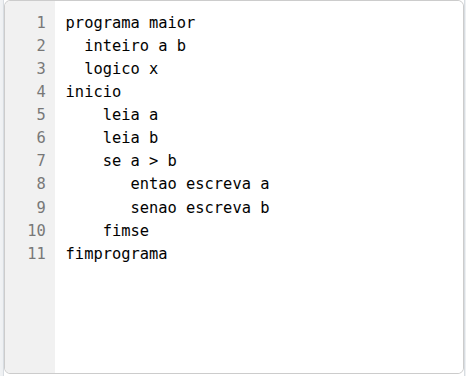
\includegraphics[width=0.5\linewidth,height=\textheight,keepaspectratio]{chapters/images/program.png}

}

\caption{\label{fig-program}Programa exemplo em linguagens simples}

\end{figure}%

A estrutura hierárquica correspondente pode ser representada por uma
árvore sintática, como ilustrado na Figura~\ref{fig-syntaxtree}.

\begin{figure}

\centering{

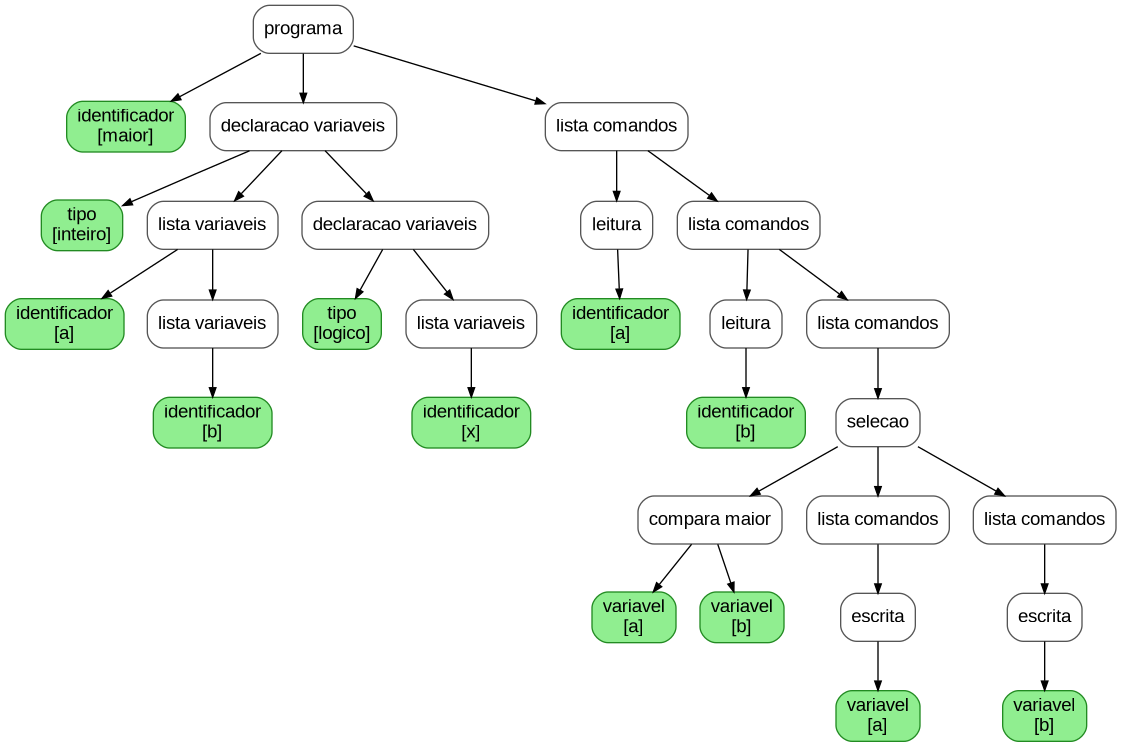
\includegraphics[width=1\linewidth,height=\textheight,keepaspectratio]{chapters/images/syntaxtree.png}

}

\caption{\label{fig-syntaxtree}Árvore sintática do programa que calcula
o maior valor}

\end{figure}%

A árvore permite visualizar a relação entre as diferentes construções do
programa. A raiz representa o programa como um todo, enquanto os nós
internos representam construções sintáticas e as folhas correspondem, em
uma representação concreta, aos elementos terminais da linguagem.

Em implementações modernas, é comum utilizar uma \textbf{árvore
sintática abstrata} (\emph{Abstract Syntax Tree} -- AST), que elimina
detalhes sintáticos que não são necessários às etapas posteriores. A AST
fornece uma representação mais compacta e adequada para a análise
semântica, otimização e geração de código.

A ferramenta \emph{bison} será utilizada neste curso para auxiliar na
construção do analisador sintático. A partir da especificação de uma
gramática livre de contexto e das ações associadas às suas produções, o
\emph{bison} gera o código necessário para realizar o processo de
análise sintática.

\subsection{Análise semântica}\label{anuxe1lise-semuxe2ntica}

A \textbf{análise semântica} é a fase na qual o compilador verifica
propriedades relacionadas ao significado das construções sintáticas
reconhecidas. Uma construção pode estar sintaticamente correta e, mesmo
assim, apresentar um erro semântico.

Considere, por exemplo, uma atribuição:

\begin{Shaded}
\begin{Highlighting}[]
\NormalTok{A := B + C;}
\end{Highlighting}
\end{Shaded}

A construção pode estar corretamente formada segundo a gramática da
linguagem. Entretanto, para determinar se ela é válida, é necessário
conhecer os tipos de \texttt{A}, \texttt{B} e \texttt{C}, bem como as
regras de compatibilidade de tipos da linguagem.

Entre as verificações realizadas durante a análise semântica
encontram-se:

\begin{enumerate}
\def\labelenumi{\arabic{enumi}.}
\item
  \textbf{Compatibilidade de tipos.} Verifica se os tipos envolvidos em
  operações e atribuições são compatíveis com as regras da linguagem.
\item
  \textbf{Declaração e uso de identificadores.} Verifica se variáveis,
  constantes, funções, procedimentos e outros identificadores utilizados
  no programa foram devidamente declarados.
\item
  \textbf{Regras de escopo e visibilidade.} Determina qual declaração de
  um identificador deve ser utilizada em cada ponto do programa,
  respeitando as regras de escopo da linguagem.
\item
  \textbf{Compatibilidade entre declarações e usos.} Verifica se uma
  entidade está sendo utilizada de acordo com sua categoria e
  declaração. Por exemplo, uma variável declarada como vetor não deve
  ser utilizada como se fosse um registro.
\item
  \textbf{Referências a entidades.} Verifica se referências presentes no
  programa correspondem a entidades válidas. Por exemplo, um
  identificador utilizado em uma expressão deve corresponder a uma
  declaração acessível naquele contexto.
\end{enumerate}

A análise semântica normalmente utiliza informações armazenadas na
tabela de símbolos. Dessa forma, as fases léxica, sintática e semântica
não são completamente independentes. O analisador léxico identifica os
nomes, o analisador sintático determina a estrutura na qual esses nomes
aparecem e o analisador semântico verifica se seu uso é consistente com
as regras da linguagem.

\subsection{Tratamento de erros}\label{tratamento-de-erros}

Um compilador deve ser capaz não apenas de reconhecer programas válidos,
mas também de detectar e comunicar adequadamente os erros encontrados
durante a compilação. Essa característica é especialmente importante em
ambientes de desenvolvimento, nos quais o usuário espera receber
informações que auxiliem na correção do programa.

Os erros podem ser classificados de acordo com a fase em que são
identificados. Um caractere inválido pode produzir um erro léxico; uma
sequência incorreta de \emph{tokens} pode produzir um erro sintático; e
uma operação envolvendo tipos incompatíveis pode produzir um erro
semântico.

Quando um erro é identificado, o módulo de tratamento de erros deve
produzir uma mensagem que permita compreender sua causa e, quando
possível, sua localização no programa fonte. Informações como número da
linha, posição aproximada e descrição do problema são particularmente
úteis.

Após identificar um erro, existem duas estratégias gerais. A primeira é
interromper o processo de compilação, estratégia conhecida como
\textbf{modo de pânico}. É uma abordagem simples e adequada quando a
continuação da análise não é segura ou quando não se deseja realizar
recuperação de erros.

A segunda estratégia consiste em tentar \textbf{recuperar-se do erro},
permitindo que a análise continue. Nesse caso, o compilador procura
determinar um ponto a partir do qual possa continuar o processamento sem
comprometer completamente a análise das construções seguintes.

A recuperação de erros é importante porque permite identificar vários
problemas em uma única execução do compilador. Em vez de corrigir um
erro, recompilar o programa e somente então descobrir o próximo, o
programador pode receber um conjunto de mensagens referentes a
diferentes problemas encontrados no código.

\subsection{Geração de código
intermediário}\label{gerauxe7uxe3o-de-cuxf3digo-intermediuxe1rio}

Entre a análise do programa fonte e a geração do código para a
máquina-alvo, o compilador pode utilizar uma representação
intermediária. Essa representação facilita a separação entre as
características da linguagem fonte e as características da plataforma de
execução.

Uma representação intermediária deve ser suficientemente expressiva para
representar as construções da linguagem, mas, ao mesmo tempo,
suficientemente simples para permitir sua análise e transformação.
Existem diversas formas de representação intermediária, como árvores,
grafos e representações baseadas em instruções de três endereços.

Uma representação simples para expressões aritméticas é a utilização de
\textbf{quádruplas}. Considere a atribuição:

\begin{Shaded}
\begin{Highlighting}[]
\NormalTok{A := (B + C) * (D + E);}
\end{Highlighting}
\end{Shaded}

Uma possível representação por quádruplas é:

\begin{longtable*}[]{|c|c|c|c|}
\toprule\noalign{}
Operador & Argumento 1 & Argumento 2 & Resultado \\
\midrule\noalign{}
\endhead
\bottomrule\noalign{}
\endlastfoot
\texttt{+} & \texttt{B} & \texttt{C} & \texttt{T1} \\
\midrule
\texttt{+} & \texttt{D} & \texttt{E} & \texttt{T2} \\
\midrule
\texttt{*} & \texttt{T1} & \texttt{T2} & \texttt{A} \\
\end{longtable*}

As variáveis temporárias \texttt{T1} e \texttt{T2} representam
resultados intermediários. A primeira quádrupla calcula
\texttt{B\ +\ C}; a segunda calcula \texttt{D\ +\ E}; e a terceira
multiplica os dois resultados e armazena o valor em \texttt{A}.

A representação intermediária facilita a realização de otimizações, pois
permite analisar as operações do programa sem depender diretamente das
instruções específicas do processador. Posteriormente, essa
representação pode ser convertida para o código da máquina-alvo.

\subsection{Otimização de código}\label{otimizauxe7uxe3o-de-cuxf3digo}

A \textbf{otimização de código} consiste na aplicação de transformações
que procuram melhorar as características do programa gerado, sem alterar
seu comportamento observável. Entre os objetivos mais comuns estão a
redução do tempo de execução e a redução da quantidade de memória
necessária.

Uma otimização importante é a \textbf{eliminação de subexpressões
comuns}. Considere, por exemplo:

\begin{Shaded}
\begin{Highlighting}[]
\NormalTok{C := (A + B) * (A + B);}
\end{Highlighting}
\end{Shaded}

A expressão \texttt{A\ +\ B} aparece duas vezes, mas seu valor pode ser
calculado uma única vez e reutilizado:

\begin{Shaded}
\begin{Highlighting}[]
\NormalTok{T1 := A + B}
\NormalTok{C := T1 * T1}
\end{Highlighting}
\end{Shaded}

Essa transformação evita a realização de uma operação que produziria
novamente um valor já conhecido.

Outra possibilidade é a \textbf{eliminação de saltos desnecessários}.
Durante a tradução de estruturas condicionais e de repetição, podem ser
produzidas sequências de instruções de desvio que não são necessárias. A
otimização pode simplificar essas sequências, reduzindo o número de
instruções executadas.

Também é possível realizar a \textbf{movimentação de código invariante
de laço}. Uma expressão ou atribuição que produz sempre o mesmo
resultado em todas as iterações de uma repetição pode, em determinadas
condições, ser executada antes do início do laço.

Considere:

\begin{Shaded}
\begin{Highlighting}[]
\NormalTok{i := }\DecValTok{1}\NormalTok{;}
\KeywordTok{repeat}
\NormalTok{    J := X;}
\NormalTok{    i := i + }\DecValTok{1}\NormalTok{;}
\KeywordTok{until}\NormalTok{ i \textgreater{}= }\DecValTok{100}\NormalTok{;}
\end{Highlighting}
\end{Shaded}

Se a expressão \texttt{J\ :=\ X} não depender de valores modificados
durante a repetição e não possuir efeitos colaterais que impeçam a
transformação, ela poderá ser deslocada para antes do laço:

\begin{Shaded}
\begin{Highlighting}[]
\NormalTok{J := X;}
\NormalTok{i := }\DecValTok{1}\NormalTok{;}
\KeywordTok{repeat}
\NormalTok{    i := i + }\DecValTok{1}\NormalTok{;}
\KeywordTok{until}\NormalTok{ i \textgreater{}= }\DecValTok{100}\NormalTok{;}
\end{Highlighting}
\end{Shaded}

Essa transformação elimina a repetição desnecessária da atribuição.

As otimizações podem ser realizadas em diferentes níveis. Algumas
dependem apenas da estrutura lógica do programa e podem ser realizadas
independentemente do processador. Outras dependem das características da
arquitetura da máquina-alvo e, portanto, são realizadas em uma etapa
mais próxima da geração do código final.

\subsubsection{Otimização local}\label{otimizauxe7uxe3o-local}

A \textbf{otimização local} considera características específicas do
código produzido para uma determinada arquitetura. Nesse nível, o
compilador pode utilizar informações sobre o conjunto de instruções, os
registradores disponíveis, os modos de endereçamento e outras
características do processador-alvo.

Por exemplo, uma sequência de operações da representação intermediária
pode ser substituída por uma instrução específica do processador que
realize a mesma tarefa com menor número de instruções.

A otimização local é, portanto, fortemente dependente da arquitetura
para a qual o código está sendo gerado. Essa característica estabelece
uma separação importante entre as otimizações independentes da máquina e
aquelas que exploram características específicas do ambiente de
execução.

\subsection{Geração de código
objeto}\label{gerauxe7uxe3o-de-cuxf3digo-objeto}

A \textbf{geração de código} é a etapa responsável por transformar a
representação intermediária em uma representação adequada à
máquina-alvo. O gerador de código precisa escolher instruções e formas
de representação que implementem corretamente as operações identificadas
nas fases anteriores.

Entre suas responsabilidades estão a seleção de instruções, a utilização
dos registradores, o cálculo de endereços e a organização das operações
de acordo com as características da arquitetura-alvo.

O resultado dessa etapa pode ser um arquivo contendo código objeto,
código de máquina ou outra forma de representação que será
posteriormente utilizada pelo sistema de execução. Em muitos ambientes,
o código produzido pelo compilador ainda precisa passar por etapas
adicionais, como a ligação com bibliotecas e outros módulos, antes que
seja obtido um programa executável.

Essa organização permite separar os problemas relacionados ao
reconhecimento e à compreensão do programa daqueles relacionados à sua
implementação em uma determinada plataforma. Ao longo deste livro, essas
etapas serão estudadas individualmente, com ênfase na construção dos
analisadores léxico e sintático e na utilização das ferramentas
\emph{flex} e \emph{bison}.

\section{Ferramentas para construção do
compilador}\label{ferramentas-para-construuxe7uxe3o-do-compilador}

A construção manual de todas as etapas de um compilador é uma tarefa
extensa. Por isso, ferramentas especializadas podem ser utilizadas para
automatizar partes do processo.

Neste curso, o \emph{flex} será utilizado para a construção do
analisador léxico. A especificação fornecida ao \emph{flex} descreve
padrões que correspondem às unidades léxicas da linguagem. Esses padrões
são normalmente expressos por meio de expressões regulares. A partir
deles, a ferramenta gera código para reconhecer as sequências de
caracteres correspondentes.

O funcionamento do \emph{flex} pode ser compreendido a partir do
conceito de autômatos finitos. Os padrões especificados pelo programador
são convertidos em uma estrutura capaz de reconhecer as cadeias
pertencentes às linguagens regulares correspondentes. O código gerado
realiza, então, a varredura do programa fonte e produz os \emph{tokens}
que serão utilizados pelo analisador sintático.

Para a construção do analisador sintático será utilizado o \emph{bison}.
Nele, o programador especifica a gramática da linguagem por meio de
produções e pode associar ações semânticas às regras. A ferramenta gera
o código necessário para realizar o processo de análise sintática.

O analisador gerado pelo \emph{bison} utiliza uma estratégia de análise
baseada em uma pilha e em uma tabela de decisões. Assim, a construção do
analisador pode ser relacionada aos conceitos de gramáticas livres de
contexto e autômatos com pilha.

A combinação dessas duas ferramentas estabelece uma arquitetura na qual
o \emph{flex} é responsável pelo reconhecimento das unidades léxicas e o
\emph{bison} pela análise da organização dessas unidades segundo a
gramática da linguagem. O resultado é uma cadeia de processamento na
qual o analisador léxico fornece os \emph{tokens} ao analisador
sintático, que, por sua vez, coordena as ações necessárias para a
construção e o processamento das estruturas do programa.

\bookmarksetup{startatroot}

\chapter{Fundamentos Matemáticos}\label{fundamentos-matemuxe1ticos}

\begin{center}
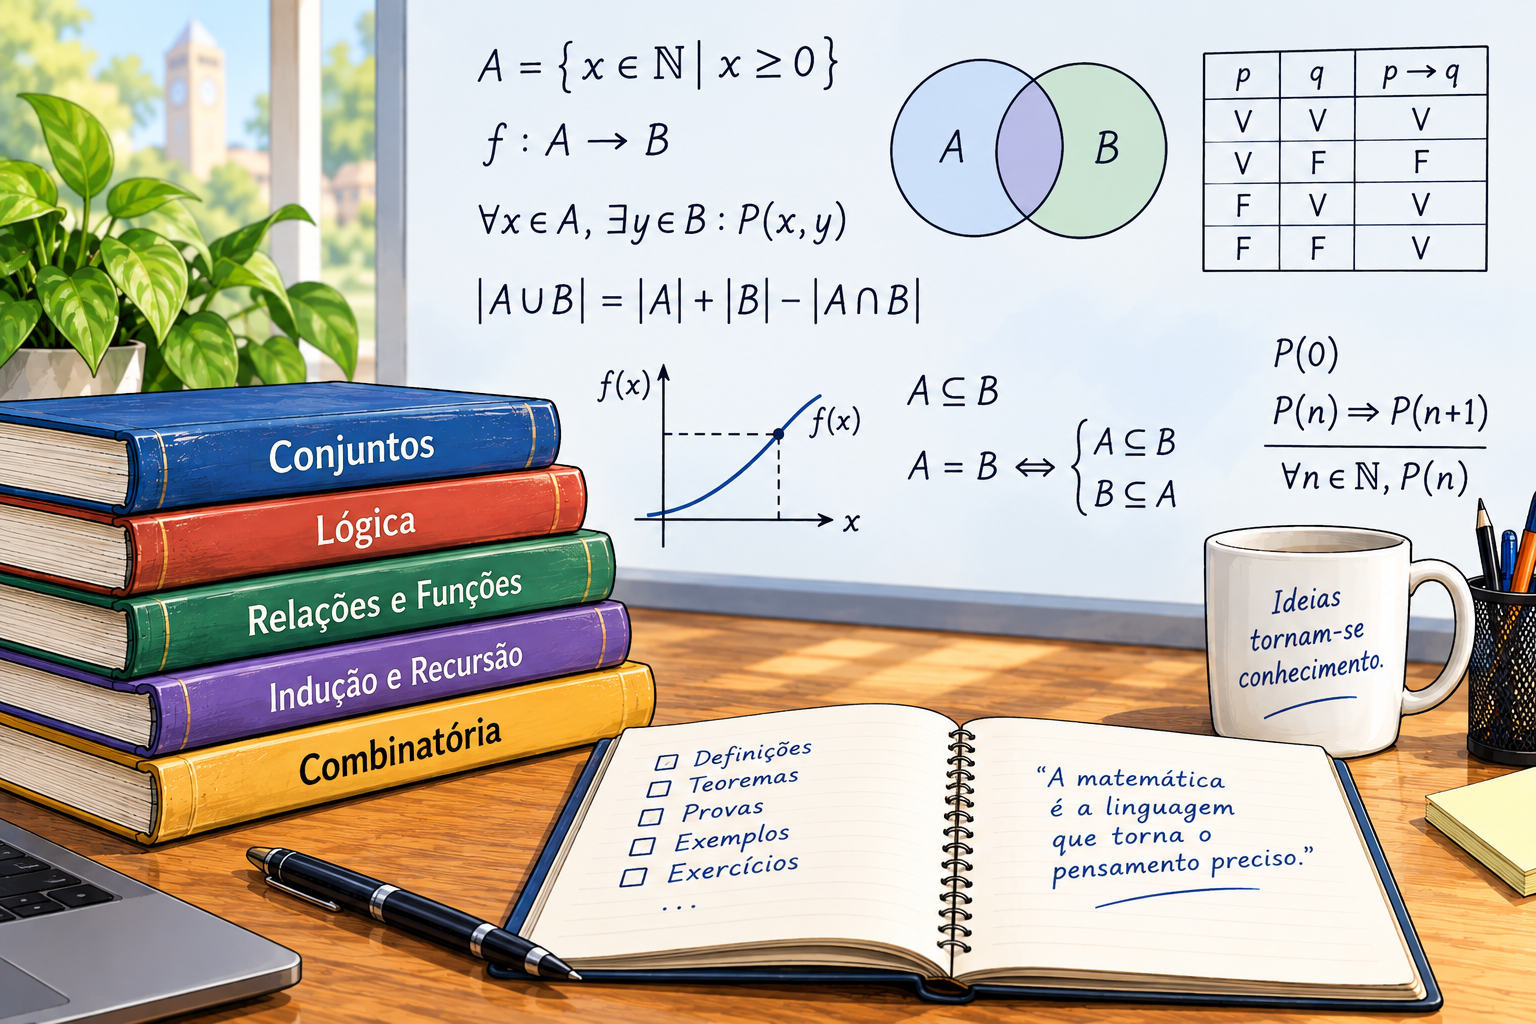
\includegraphics[width=0.7\linewidth,height=\textheight,keepaspectratio]{chapters/images/fundamentos.png}
\end{center}

O estudo da \textbf{Teoria de Linguagens e Autômatos} utiliza uma série
de conceitos matemáticos que permitem descrever, de maneira precisa e
formal, os objetos computacionais e as relações existentes entre eles.
Embora muitos desses conceitos sejam elementares e façam parte da
formação matemática básica, é importante apresentá-los e estabelecer sua
notação antes de iniciar as definições formais da teoria.

Essa formalização é particularmente importante porque, ao longo do
estudo, serão utilizados conceitos matemáticos para definir
\textbf{alfabetos, palavras, linguagens, autômatos, funções de transição
e relações}. Além disso, diversas propriedades dos modelos
computacionais serão demonstradas matematicamente. Para que essas
definições e demonstrações possam ser compreendidas sem ambiguidades, é
necessário estabelecer previamente o significado dos principais objetos
e operações matemáticas utilizados.

Entre os conceitos fundamentais, os \textbf{conjuntos} ocupam uma
posição central. Praticamente todos os objetos da Teoria de Linguagens
podem ser definidos a partir deles ou representados como conjuntos. Um
alfabeto, por exemplo, pode ser entendido como um conjunto finito de
símbolos, enquanto uma linguagem pode ser definida como um conjunto de
palavras. Da mesma forma, os estados de um autômato e suas transições
podem ser organizados e manipulados utilizando operações sobre
conjuntos.

\section{Conjuntos}\label{conjuntos}

Um \textbf{conjunto} é uma coleção de objetos que são tratados como uma
única entidade. Esses objetos são denominados \textbf{elementos} do
conjunto. Os elementos podem ser de diferentes naturezas: números,
símbolos, palavras, estados de um autômato ou até mesmo outros
conjuntos.

Por exemplo, podemos considerar o conjunto formado pelos números 2, 4 e
12:

\[
A = \{2,4,12\}
\]

Também é possível definir um conjunto por meio de uma propriedade que
caracteriza seus elementos. Essa forma de representação é
particularmente útil quando o conjunto possui muitos elementos ou é
infinito. Por exemplo, o conjunto dos números pares pode ser definido
por:

\[
pares = \{n \mid n = 2m,; m \in \mathbb{N}\}
\]

A expressão significa que o conjunto é formado por todos os elementos
\(n\) que podem ser escritos como duas vezes algum número natural \(m\).

Para indicar que um elemento pertence a um conjunto, utiliza-se o
símbolo \(\in\). Por exemplo:

\[
7 \in \{1,7,34\}
\]

Essa expressão deve ser lida como ``7 pertence ao conjunto
\({1,7,34}\)''. Quando um elemento não pertence a um conjunto,
utiliza-se o símbolo \(\notin\). Assim, podemos escrever:

\[
5 \notin \{1,7,34\}
\]

Essa notação de pertencimento será utilizada frequentemente na Teoria de
Linguagens. Por exemplo, quando definirmos um alfabeto \(\Sigma\),
poderemos escrever \(a \in \Sigma\) para indicar que o símbolo \(a\)
pertence ao alfabeto.

\subsection{Subconjuntos}\label{subconjuntos}

Além de analisar a relação entre um elemento e um conjunto, é possível
analisar a relação entre dois conjuntos. Dizemos que um conjunto \(A\) é
\textbf{subconjunto} de um conjunto \(B\) quando todos os elementos de
\(A\) também pertencem a \(B\). Essa relação é representada por:

\[
A \subseteq B
\]

Quando, além disso, \(A\) possui menos elementos que \(B\), isto é,
existe pelo menos um elemento de \(B\) que não pertence a \(A\),
utilizamos a notação:

\[
A \subsetneq B
\]

para indicar que \(A\) é um \textbf{subconjunto próprio} de \(B\).

É importante observar que, em um conjunto, a ordem em que os elementos
são apresentados não possui significado. Da mesma forma, a repetição de
um elemento não altera o conjunto. Assim:

\[
\{1,2,3\} = \{3,2,1\}
\]

e

\[
\{1\} = \{1,1\}
\]

Quando a quantidade de ocorrências de cada elemento é relevante, não
estamos mais trabalhando com conjuntos no sentido tradicional, mas com
uma estrutura denominada \textbf{multiconjunto}.

Os conjuntos também podem ser finitos ou infinitos. Um conjunto finito
possui uma quantidade limitada de elementos. Já um conjunto infinito
possui uma quantidade ilimitada de elementos. Os números naturais, por
exemplo, formam um conjunto infinito:

\[
\mathbb{N} = \{0,1,2,3,\ldots\}
\]

Da mesma forma, o conjunto dos números inteiros é infinito:

\[
\mathbb{Z} = \{\ldots,-2,-1,0,1,2,\ldots\}
\]

A distinção entre conjuntos finitos e infinitos será importante
posteriormente, especialmente quando forem discutidas propriedades dos
alfabetos, das linguagens e dos diferentes modelos de autômatos.

\subsection{Operações com
Conjuntos}\label{operauxe7uxf5es-com-conjuntos}

Além das relações de pertencimento e inclusão, os conjuntos podem ser
combinados por meio de diferentes operações. Essas operações permitem
construir novos conjuntos a partir de conjuntos existentes e serão
utilizadas posteriormente na definição e manipulação de linguagens
formais.

\subsubsection{União}\label{uniuxe3o}

\begin{figure}

\centering{

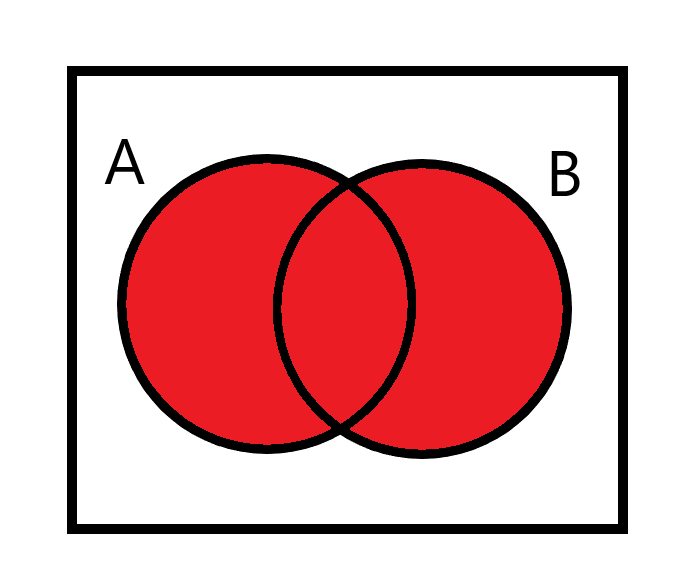
\includegraphics[width=0.3\linewidth,height=\textheight,keepaspectratio]{chapters/images/uniao.png}

}

\caption{\label{fig-uniao}Representação da união de conjuntos}

\end{figure}%

A \textbf{união} de dois conjuntos \(A\) e \(B\) é formada por todos os
elementos que pertencem a pelo menos um dos conjuntos. A união é
representada pelo símbolo \(\cup\):

\[
A \cup B = \{x \mid x \in A \textrm{ ou } x \in B\}
\]

Por exemplo, considerando:

\[
A = \{1,2,3\}
\]

e

\[
B = \{3,4,5\}
\]

temos:

\[
A \cup B = \{1,2,3,4,5\}
\]

Observe que o elemento 3 aparece apenas uma vez no resultado, pois
conjuntos não consideram repetições.

A operação de união possui especial importância na Teoria de Linguagens,
pois será utilizada posteriormente na definição da \textbf{união de
linguagens} e estará diretamente relacionada à operação de união de
autômatos.

\subsubsection{Interseção}\label{interseuxe7uxe3o}

\begin{figure}

\centering{

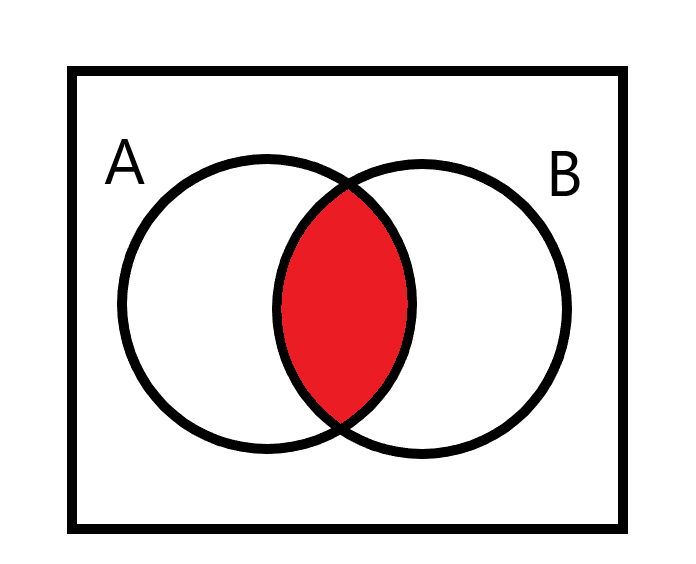
\includegraphics[width=0.3\linewidth,height=\textheight,keepaspectratio]{chapters/images/intersecao.png}

}

\caption{\label{fig-intersecao}Representação da interseção entre
conjuntos}

\end{figure}%

A \textbf{interseção} de dois conjuntos contém os elementos que
pertencem simultaneamente aos dois conjuntos. A operação é representada
pelo símbolo \(\cap\):

\[
A \cap B = \{x \mid x \in A \textrm{ e } x \in B\}
\]

Por exemplo, para:

\[
A = \{1,2,3\}
\]

e

\[
B = \{3,4,5\}
\]

temos:

\[
A \cap B = \{3\}
\]

A interseção permite representar uma condição em que um elemento precisa
satisfazer simultaneamente duas propriedades. Esse conceito será
importante posteriormente na construção de linguagens que representam
condições combinadas.

\subsubsection{Diferença}\label{diferenuxe7a}

\begin{figure}

\centering{

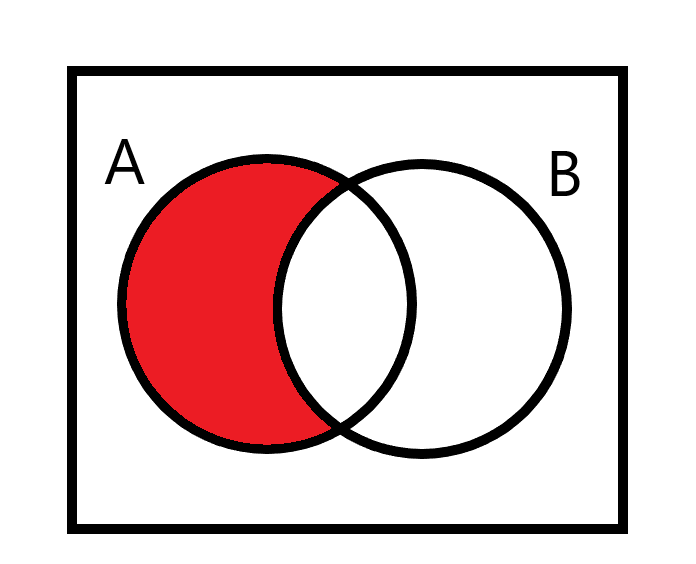
\includegraphics[width=0.3\linewidth,height=\textheight,keepaspectratio]{chapters/images/diferenca.png}

}

\caption{\label{fig-diferenca}Representação da diferença de conjuntos}

\end{figure}%

A \textbf{diferença} entre dois conjuntos \(A\) e \(B\) é formada pelos
elementos que pertencem a \(A\), mas não pertencem a \(B\). A operação
pode ser representada por \(A-B\):

\[
A - B = \{x \mid x \in A \textrm{ e } x \notin B\}
\]

Por exemplo:

\[
A = \{1,2,3,4\}
\]

e

\[
B = \{3,4,5\}
\]

resultam em:

\[
A-B = \{1,2\}
\]

A diferença é uma operação útil para expressar a remoção de elementos de
um conjunto e será retomada posteriormente em diferentes construções da
teoria.

\subsubsection{Importância dos conjuntos para a Teoria de
Linguagens}\label{importuxe2ncia-dos-conjuntos-para-a-teoria-de-linguagens}

Os conceitos apresentados nesta seção constituem uma base para
praticamente todas as definições que serão introduzidas posteriormente.
Um \textbf{alfabeto} será definido como um conjunto de símbolos; uma
\textbf{palavra} será construída a partir de símbolos pertencentes a um
alfabeto; e uma \textbf{linguagem} poderá ser definida como um conjunto
de palavras.

Da mesma forma, um autômato será descrito por conjuntos de
\textbf{estados}, \textbf{símbolos} e \textbf{transições}, além de
funções que estabelecem relações entre esses elementos. As operações de
união, interseção, diferença e inclusão também serão utilizadas para
estabelecer propriedades das linguagens e demonstrar resultados
importantes.

Portanto, esta revisão não tem apenas o objetivo de recordar conceitos
matemáticos conhecidos. Ela estabelece a \textbf{linguagem formal} que
será utilizada ao longo do livro. A partir desses fundamentos, será
possível apresentar as definições da Teoria de Linguagens de maneira
rigorosa e, posteriormente, utilizar essas definições em demonstrações,
construções de autômatos e análise das propriedades das linguagens
formais.

\section{Sequências e Uplas}\label{sequuxeancias-e-uplas}

Enquanto um conjunto é uma coleção de elementos na qual a ordem e a
repetição não são relevantes, uma \textbf{sequência} é uma lista de
objetos na qual a ordem em que os elementos aparecem é parte fundamental
da representação. Assim, em uma sequência, cada elemento ocupa uma
determinada posição. Por exemplo, podemos considerar a sequência:

\[
(1,4,20)
\]

Nesse caso, o primeiro elemento é \(1\), o segundo é \(4\) e o terceiro
é \(20\). A sequência é representada utilizando parênteses, justamente
para diferenciá-la da representação usual de conjuntos. A ordem dos
elementos produz sequências diferentes. Portanto,

\[
(1,4,20) \neq (4,1,20).
\]

Essa característica será particularmente importante no estudo das
linguagens formais, pois uma palavra pode ser entendida como uma
\textbf{sequência finita de símbolos} pertencentes a um alfabeto. Assim,
as sequências fornecem a estrutura matemática necessária para
representar a ordem em que os símbolos aparecem em uma palavra.

As sequências podem ser \textbf{finitas ou infinitas}. Uma sequência
finita possui uma quantidade determinada de elementos e é denominada
\textbf{tupla}. Uma \(k\)-upla é uma sequência constituída por \(k\)
elementos. Por exemplo,

\[
(2,1,3)
\]

é uma 3-upla, enquanto

\[
(1,2)
\]

é uma 2-upla. A posição ocupada por cada elemento é importante: a
primeira componente de uma tupla é diferente da segunda, mesmo quando os
valores envolvidos são iguais.

\subsection{Conjunto das partes}\label{conjunto-das-partes}

É importante observar que conjuntos e sequências podem ser utilizados
como elementos de outras estruturas matemáticas. Por exemplo, considere
o conjunto:

\[
A=\{0,1\}.
\]

O \textbf{conjunto das partes}, ou \textbf{conjunto potência}, de \(A\)
é o conjunto formado por todos os subconjuntos de \(A\). Nesse caso,
temos:

\[
P(A)=\{\emptyset,\{0\},\{1\},\{0,1\}\}.
\]

Esse exemplo mostra que os próprios conjuntos podem aparecer como
elementos de outro conjunto. De maneira semelhante, tuplas podem conter
conjuntos, sequências ou outros objetos matemáticos como seus
componentes. Essa possibilidade será importante quando forem definidas
estruturas mais complexas utilizadas na representação de autômatos e de
outros modelos computacionais.

\subsection{Produto cartesiano}\label{produto-cartesiano}

Outro conceito fundamental relacionado aos conjuntos e às sequências é o
\textbf{produto cartesiano}. Dados dois conjuntos \(A\) e \(B\), o
produto cartesiano, denotado por \(A\times B\), é o conjunto formado por
todos os pares ordenados \((a,b)\) nos quais \(a\in A\) e \(b\in B\).

Por exemplo, sejam:

\[
A=\{1,2\}
\]

e

\[
B=\{x,y,z\}.
\]

O produto cartesiano desses conjuntos é:

\[
A\times B=
\{(1,x),(1,y),(1,z),(2,x),(2,y),(2,z)\}.
\]

Cada elemento do produto cartesiano é, portanto, uma \textbf{2-upla}, ou
par ordenado. Observe novamente que a ordem é importante. Em geral,

\[
(a,b)\neq(b,a),
\]

pois a primeira componente pertence a \(A\) e a segunda pertence a
\(B\).

O produto cartesiano pode ser estendido para mais de dois conjuntos.
Dados os conjuntos \(A_1,A_2,\ldots,A_k\), podemos definir:

\[
A_1\times A_2\times\cdots\times A_k
\]

como o conjunto formado por todas as \(k\)-uplas

\[
(a_1,a_2,\ldots,a_k),
\]

nas quais cada componente pertence ao respectivo conjunto:

\[
a_i\in A_i.
\]

Essa definição permite representar matematicamente estruturas que
possuem diferentes componentes organizados em posições específicas.

Quando todos os conjuntos envolvidos no produto cartesiano são iguais,
podemos utilizar uma notação abreviada. O produto cartesiano de \(A\)
por ele mesmo \(k\) vezes é representado por:

\[
\underbrace{A\times A\times\cdots\times A}_{k\text{ vezes}}
=A^k.
\]

Por exemplo:

\[
\mathbb{N}^2=\mathbb{N}\times\mathbb{N}
\]

representa o conjunto de todos os pares ordenados de números naturais.
Assim:

\[
\mathbb{N}^2=
\{(0,0),(0,1),(0,2),\ldots,(1,0),(1,1),\ldots\}.
\]

O conceito de produto cartesiano será utilizado posteriormente para
formalizar diversas estruturas da Teoria de Linguagens. Em particular,
ele permite definir conjuntos de tuplas e estabelecer relações entre
diferentes conjuntos de objetos. Dessa forma, sequências, tuplas e
produtos cartesianos complementam os conceitos de conjuntos apresentados
anteriormente e fornecem uma base matemática para a definição formal de
alfabetos, palavras, linguagens e autômatos.

\section{Funções e Relações}\label{funuxe7uxf5es-e-relauxe7uxf5es}

Funções e relações são conceitos fundamentais da Matemática Discreta e
aparecem de maneira recorrente na definição dos objetos estudados em
Teoria de Linguagens. Autômatos, gramáticas e linguagens formais são
definidos a partir de conjuntos e operações entre seus elementos. Para
compreender adequadamente essas definições, é importante conhecer como
funções e relações permitem representar transformações, propriedades e
comparações entre objetos.

\subsection{Funções}\label{funuxe7uxf5es}

Uma \textbf{função} é uma regra que associa elementos de um conjunto de
entrada a elementos de um conjunto de saída. Formalmente, uma função
\(f\) de um conjunto \(D\) em um conjunto \(C\) é representada por

\[
f:D\rightarrow C.
\]

O conjunto \(D\) é denominado \textbf{domínio} da função e o conjunto
\(C\) é denominado \textbf{contradomínio}. Para cada elemento
\(a\in D\), a função associa exatamente um elemento \(b\in C\). Essa
associação é indicada por

\[
f(a)=b.
\]

A exigência de que cada elemento do domínio esteja associado a
exatamente um elemento do contradomínio é o que diferencia uma função de
uma relação arbitrária. Um mesmo elemento do contradomínio pode ser
associado a vários elementos do domínio; portanto, não é necessário que
elementos diferentes do domínio tenham imagens diferentes.

Uma função também pode ser denominada \textbf{mapeamento}, pois
estabelece uma correspondência entre elementos de dois conjuntos. Por
exemplo, considere a função

\[
add:\mathbb{Z}\times\mathbb{Z}\rightarrow\mathbb{Z},
\]

definida por

\[
add(x,y)=x+y.
\]

Nesse caso, o domínio é o produto cartesiano
\(\mathbb{Z}\times\mathbb{Z}\), o contradomínio é \(\mathbb{Z}\) e a
função possui dois argumentos. Assim, a entrada da função é um par
ordenado \((x,y)\).

De maneira geral, uma função pode possuir qualquer número finito de
argumentos. Uma função

\[
f:A_1\times A_2\times\cdots\times A_k\rightarrow B
\]

recebe como entrada uma \(k\)-upla

\[
(a_1,a_2,\ldots,a_k),
\]

em que cada \(a_i\) pertence ao conjunto correspondente \(A_i\). Uma
função com um argumento é denominada \textbf{função unária}, enquanto
uma função com dois argumentos é denominada \textbf{função binária}.
Essa terminologia será utilizada diversas vezes ao longo do estudo de
linguagens formais.

Uma função pode ser representada de diferentes maneiras. Podemos
utilizar uma expressão matemática, uma tabela, um diagrama ou até mesmo
um algoritmo ou programa de computador. Considere, por exemplo, a função

\[
f:\mathbb{Z}_5\rightarrow\mathbb{Z}_5
\]

definida por

\[
f(x)=(x+1)\bmod 5.
\]

Como \(\mathbb{Z}_5={0,1,2,3,4}\), podemos representar essa função pela
tabela:

\begin{longtable*}[]{|c|c|c|c|c|c|}
\toprule\noalign{}
\(x\) & 0 & 1 & 2 & 3 & 4 \\
\midrule\noalign{}
\endhead
\bottomrule\noalign{}
\endlastfoot
\(f(x)\) & 1 & 2 & 3 & 4 & 0 \\
\end{longtable*}

Observe que cada elemento do domínio possui exatamente uma imagem.
Assim, \(f(0)=1\), \(f(1)=2\), \(f(2)=3\), \(f(3)=4\) e \(f(4)=0\). O
uso da operação módulo faz com que, depois do valor \(4\), o resultado
volte para \(0\).

Essa forma de representar funções é particularmente útil em Computação.
Uma tabela de transição de um autômato, por exemplo, pode ser entendida
como uma representação tabular de uma função. Essa observação permite
estabelecer uma conexão direta entre o conceito matemático de função e a
definição formal dos autômatos.

\subsection{Predicados}\label{predicados}

Outro conceito importante relacionado às funções é o de
\textbf{predicado}. Um predicado, também denominado
\textbf{propriedade}, é uma função cujo contradomínio possui dois
valores possíveis, normalmente representados por verdadeiro e falso.

Um exemplo simples é o predicado que determina se um número inteiro é
par. Podemos defini-lo como

\[
par:\mathbb{Z}\rightarrow\{\text{verdadeiro},\text{falso}\},
\]

em que

\[
par(x)=
\begin{cases}
\text{verdadeiro}, & \text{se }x\bmod 2=0,\\
\text{falso}, & \text{caso contrário}.
\end{cases}
\]

Assim, \(par(4)\) é verdadeiro, enquanto \(par(5)\) é falso.

Os predicados são particularmente importantes em Teoria de Linguagens
porque uma linguagem pode ser interpretada como uma propriedade sobre as
cadeias de um alfabeto. Seja

\[
L\subseteq\Sigma^*
\]

uma linguagem. Podemos definir o predicado

\[
P_L:\Sigma^*\rightarrow\{\text{verdadeiro},\text{falso}\}
\]

por

\[
P_L(w)=
\begin{cases}
\text{verdadeiro}, & \text{se }w\in L,\\
\text{falso}, & \text{se }w\notin L.
\end{cases}
\]

Nesse caso, o predicado \(P_L\) responde à pergunta fundamental:
\textbf{a cadeia} \(w\) pertence à linguagem \(L\)?

Essa interpretação permite compreender o papel de um reconhecedor de
linguagens. Um autômato recebe uma cadeia como entrada e produz, ao
final do processamento, uma resposta que pode ser interpretada como
verdadeiro ou falso. Se a cadeia é aceita, o predicado correspondente
assume o valor verdadeiro; caso contrário, assume o valor falso.

\subsection{Relações de
equivalência}\label{relauxe7uxf5es-de-equivaluxeancia}

Uma relação binária \(R\) definida sobre um conjunto \(A\) é denominada
\textbf{relação de equivalência} quando satisfaz três propriedades:
reflexividade, simetria e transitividade.

A \textbf{reflexividade} estabelece que todo elemento está relacionado
consigo mesmo. Formalmente,

\[
\forall x\in A,\quad xRx.
\]

A \textbf{simetria} estabelece que, se um elemento está relacionado a
outro, então o segundo também está relacionado ao primeiro:

\[
\forall x,y\in A,\quad
xRy\Rightarrow yRx.
\]

Finalmente, a \textbf{transitividade} estabelece que, se um elemento
está relacionado a um segundo e este está relacionado a um terceiro,
então o primeiro está relacionado ao terceiro:

\[
\forall x,y,z\in A,\quad
(xRy\land yRz)\Rightarrow xRz.
\]

A igualdade entre números é um exemplo conhecido de relação de
equivalência. Se \(x=y\), então naturalmente \(x=x\), \(y=x\) e, se
\(x=y\) e \(y=z\), então \(x=z\).

Outro exemplo é a relação de congruência módulo \(n\). Dois inteiros
\(x\) e \(y\) são considerados equivalentes módulo \(n\) quando possuem
o mesmo resto na divisão por \(n\). Essa relação permite agrupar
infinitos números inteiros em um número finito de classes.

A ideia de agrupar elementos equivalentes é extremamente importante em
Computação. Em vez de considerar individualmente todos os elementos de
um conjunto, podemos trabalhar com as \textbf{classes de equivalência}
formadas pela relação.

\subsection{Funções, predicados e relações: uma visão
integrada}\label{funuxe7uxf5es-predicados-e-relauxe7uxf5es-uma-visuxe3o-integrada}

Os conceitos apresentados nesta seção aparecem de forma integrada em
praticamente toda a Teoria de Linguagens. As funções são utilizadas para
descrever transformações e comportamentos determinísticos; os predicados
permitem expressar propriedades que podem ser verdadeiras ou falsas; e
as relações permitem estabelecer associações ou comparações entre
objetos.

\section{Grafos}\label{grafos}

Grafos são estruturas matemáticas utilizadas para representar relações
entre objetos. Um grafo pode ser utilizado, por exemplo, para
representar cidades conectadas por estradas, páginas da Web conectadas
por links, pessoas conectadas por relações sociais ou estados de um
autômato conectados por transições. Na Teoria de Linguagens, os grafos
possuem papel particularmente importante, pois permitem representar
visualmente autômatos, relações entre estados, árvores de derivação e
diversas outras estruturas.

De maneira intuitiva, um grafo é formado por um conjunto de
\textbf{vértices}, também chamados de nós, e por conexões entre esses
vértices, denominadas \textbf{arestas}. Dependendo do tipo de grafo, as
conexões podem possuir ou não uma direção, podem possuir rótulos e podem
ainda estar associadas a pesos ou outros atributos.

\subsection{Grafos não direcionados}\label{grafos-nuxe3o-direcionados}

Um \textbf{grafo não direcionado}, ou simplesmente \textbf{grafo}, é uma
estrutura formada por um conjunto de vértices e um conjunto de arestas
que conectam pares de vértices. Em um grafo não direcionado, uma aresta
que conecta os vértices \(a\) e \(b\) não possui uma direção específica.
Assim, a conexão entre \(a\) e \(b\) é a mesma que a conexão entre \(b\)
e \(a\).

Formalmente, um grafo pode ser representado pelo par

\[
G=(V,E),
\]

em que \(V\) é o conjunto de vértices e \(E\) é o conjunto de arestas.

No caso de um grafo simples não direcionado, cada aresta é representada
por um par não ordenado de vértices. Assim,

\[
\{a,b\}
\]

representa uma aresta que conecta os vértices \(a\) e \(b\). A ordem dos
elementos não é relevante, de modo que

\[
\{a,b\}=\{b,a\}.
\]

Por exemplo, considere o grafo da

\begin{figure}

\centering{

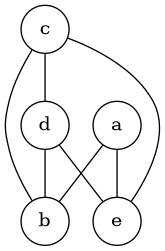
\includegraphics[width=0.2\linewidth,height=\textheight,keepaspectratio]{chapters/images/g1.png}

}

\caption{\label{fig-grafo1}Um grafo}

\end{figure}%

\[
G=(V,E),
\]

em que

\[
V=\{a,b,c,d,e\}
\]

e

\[
E=
\{
\{a,b\},
\{a,e\},
\{b,c\},
\{b,d\},
\{c,d\},
\{c,e\},
\{d,e\}
\}.
\]

Nesse grafo, os cinco elementos de \(V\) são os vértices e cada elemento
de \(E\) representa uma conexão entre dois desses vértices.

Uma representação gráfica desse grafo pode ser feita desenhando um ponto
para cada vértice e uma linha para cada aresta, conforme ilustrado na
Figura~\ref{fig-grafo1}. A representação visual é particularmente útil
porque permite identificar propriedades do grafo sem necessariamente
manipular sua representação matemática.

\subsection{Grau de um vértice}\label{grau-de-um-vuxe9rtice}

O \textbf{grau} de um vértice de um grafo não direcionado corresponde ao
número de arestas incidentes nesse vértice. Em outras palavras, indica
quantas conexões estão associadas ao vértice.

No grafo da Figura~\ref{fig-grafo1}, por exemplo, o vértice \(a\) possui
grau \(2\), pois está conectado aos vértices \(b\) e \(e\). Já o vértice
\(d\) possui grau \(3\), pois está conectado aos vértices \(b\), \(c\) e
\(e\).

O grau de um vértice pode ser representado por

\[
\deg(v).
\]

Assim, no exemplo,

\[
\deg(a)=2
\]

e

\[
\deg(d)=3.
\]

O conceito de grau é útil para caracterizar a estrutura de um grafo e
também aparece, com adaptações, no estudo de grafos direcionados.

\subsection{Grafos simples}\label{grafos-simples}

Um \textbf{grafo simples} é um grafo que não possui arestas múltiplas
entre o mesmo par de vértices e não possui arestas que conectem um
vértice a ele próprio.

Uma aresta que conecta um vértice a ele mesmo é denominada
\textbf{laço}. Por exemplo, uma aresta

\[
\{a,a\}
\]

seria um laço no vértice \(a\).

Da mesma forma, não são permitidas duas arestas distintas conectando
exatamente os mesmos dois vértices. Quando múltiplas arestas entre os
mesmos vértices são permitidas, temos estruturas mais gerais,
denominadas \textbf{multigrafos}.

A distinção entre grafos simples e grafos que permitem múltiplas arestas
ou laços é importante porque diferentes aplicações exigem diferentes
modelos. Em Teoria de Linguagens, por exemplo, os diagramas de autômatos
podem possuir várias transições entre estados e, portanto, sua
representação não precisa necessariamente ser um grafo simples.

\subsection{Grafos como modelos}\label{grafos-como-modelos}

Uma das principais aplicações dos grafos é a modelagem de sistemas. Os
vértices representam entidades e as arestas representam relações ou
conexões entre essas entidades.

\begin{figure}

\centering{

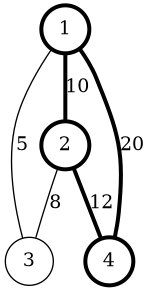
\includegraphics[width=0.15\linewidth,height=\textheight,keepaspectratio]{chapters/images/g3.png}

}

\caption{\label{fig-grafo3}Grafo como modelo}

\end{figure}%

Por exemplo, podemos utilizar um grafo para representar uma rede de
cidades, conforme ilustrado na Figura~\ref{fig-grafo3}. Nesse caso, cada
vértice representa uma cidade e cada aresta representa uma estrada que
conecta duas cidades. Outro exemplo é uma rede de páginas da Web, em que
cada vértice representa uma página e cada conexão representa um link
entre páginas.

As arestas também podem possuir \textbf{rótulos}. Nesse caso, além de
indicar que dois vértices estão relacionados, a aresta pode especificar
a natureza dessa relação. Essa característica é especialmente importante
em Teoria de Linguagens, pois as transições de um autômato são
normalmente rotuladas com símbolos do alfabeto.

Assim, uma estrutura gráfica pode representar não apenas a existência de
uma conexão, mas também a informação associada a essa conexão.

\subsection{Subgrafos}\label{subgrafos}

Um grafo pode conter dentro de sua estrutura outros grafos menores. Um
\textbf{subgrafo} de um grafo \(H\) é um grafo formado por um
subconjunto dos vértices de \(H\) e por arestas de \(H\) que conectam
esses vértices.

Se

\[
H=(V_H,E_H),
\]

um subgrafo \(G=(V_G,E_G)\) de \(H\) deve satisfazer

\[
V_G\subseteq V_H
\]

e

\[
E_G\subseteq E_H.
\]

Por exemplo, se selecionarmos os vértices \(1\), \(2\) e \(4\) do grafo
da Figura~\ref{fig-grafo3} e mantivermos as arestas existentes entre
esses vértices, obteremos um subgrafo do grafo original.

O conceito de subgrafo é útil quando estamos interessados apenas em uma
parte de uma estrutura maior. Em aplicações computacionais, isso permite
analisar regiões específicas de uma rede ou de um sistema sem considerar
todos os seus elementos.

\subsection{Caminhos}\label{caminhos}

Um dos conceitos mais importantes em grafos é o de \textbf{caminho}.
Intuitivamente, um caminho é uma sequência de vértices em que cada
vértice consecutivo está conectado por uma aresta.

Por exemplo, na Figura~\ref{fig-grafo4}

\begin{figure}

\centering{

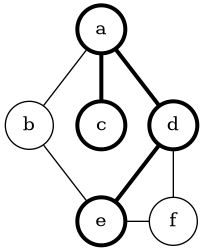
\includegraphics[width=0.2\linewidth,height=\textheight,keepaspectratio]{chapters/images/g4.png}

}

\caption{\label{fig-grafo4}Caminho num grafo}

\end{figure}%

\[
(c,a,d,e)
\]

representa um caminho quando existem as arestas

\[
\{c,a\},\quad
\{a,d\},\quad
\{d,e\}.
\]

Um caminho pode visitar um mesmo vértice mais de uma vez. Quando nenhum
vértice é repetido, temos um \textbf{caminho simples}.

O comprimento de um caminho corresponde ao número de arestas
percorridas. Assim, o caminho

\[
(a,c,d,e)
\]

possui comprimento \(3\), pois utiliza as arestas que conectam \(a\) a
\(c\), \(c\) a \(d\) e \(d\) a \(e\).

A noção de caminho é fundamental para diversas operações sobre grafos.
Ela permite, por exemplo, verificar se existe uma conexão entre dois
vértices, determinar rotas e estudar propriedades de conectividade.

\subsection{Ciclos}\label{ciclos}

Um \textbf{ciclo} é um caminho que começa e termina no mesmo vértice.
Por exemplo, conforme ilustrado na Figura~\ref{fig-grafo5}

\begin{figure}

\centering{

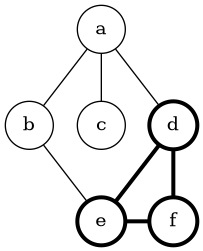
\includegraphics[width=0.2\linewidth,height=\textheight,keepaspectratio]{chapters/images/g5.png}

}

\caption{\label{fig-grafo5}Ciclo num grafo}

\end{figure}%

\[
(d,e,f,d)
\]

é um ciclo quando existem as arestas

\[
\{d,e\},\quad
\{e,f\},\quad
\{f,d\}.
\]

Um ciclo simples não repete vértices, exceto pelo primeiro e pelo
último, que são iguais.

Os ciclos são importantes porque permitem identificar situações em que é
possível retornar ao ponto de partida seguindo as conexões do grafo.
Essa propriedade terá uma interpretação particularmente importante
quando estudarmos autômatos, pois um ciclo em um autômato pode
representar a possibilidade de processar uma quantidade arbitrária de
símbolos repetindo uma determinada sequência de estados.

\subsection{Conectividade}\label{conectividade}

Um grafo é denominado \textbf{conexo} quando existe um caminho entre
quaisquer dois de seus vértices.

Considere dois vértices \(u\) e \(v\). Se existe um caminho que começa
em \(u\) e termina em \(v\), dizemos que esses vértices estão
conectados.

Um grafo desconexo possui pelo menos dois grupos de vértices que não
podem ser alcançados uns a partir dos outros. Esses grupos são
denominados \textbf{componentes conexas} do grafo.

A conectividade é uma propriedade importante em diversas aplicações. Em
uma rede de comunicação, por exemplo, um grafo conexo representa uma
rede em que existe alguma sequência de conexões entre quaisquer dois
pontos.

\subsection{Árvores}\label{uxe1rvores}

Uma \textbf{árvore} é um grafo não direcionado, conexo e sem ciclos,
conforme ilustrado na Figura~\ref{fig-grafo6}

\begin{figure}

\centering{

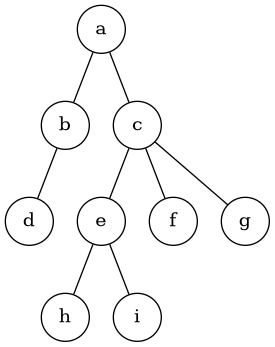
\includegraphics[width=0.3\linewidth,height=\textheight,keepaspectratio]{chapters/images/g6.png}

}

\caption{\label{fig-grafo6}Uma árvore}

\end{figure}%

Portanto, uma árvore possui duas características fundamentais: existe um
caminho entre quaisquer dois vértices e não existe um caminho que
permita sair de um vértice e retornar a ele seguindo um ciclo.

Uma propriedade importante das árvores é que, entre quaisquer dois
vértices, existe exatamente um caminho simples.

Se uma árvore possui \(n\) vértices, então ela possui exatamente

\[
n-1
\]

arestas.

As árvores aparecem frequentemente na Computação. Estruturas
hierárquicas, sistemas de arquivos, árvores de busca e árvores de
derivação de gramáticas são alguns exemplos.

Na Teoria de Linguagens, as \textbf{árvores de derivação} são utilizadas
para representar como uma cadeia pode ser gerada a partir do símbolo
inicial de uma gramática. Nesse caso, os nós da árvore representam
símbolos da gramática e a estrutura da árvore representa a sequência de
aplicações das produções.

Essa aplicação será particularmente importante no estudo de
\textbf{gramáticas livres de contexto}, em que a existência de
diferentes árvores de derivação para uma mesma cadeia pode indicar
ambiguidade da gramática.

\subsection{Grafos direcionados}\label{grafos-direcionados}

Em muitas aplicações, a existência de uma conexão entre dois objetos não
é suficiente; é necessário também indicar a direção da conexão. Nesse
caso, utilizamos um \textbf{grafo direcionado}, também chamado de
digrafo, conforme ilustrado na Figura~\ref{fig-grafo7}

\begin{figure}

\centering{

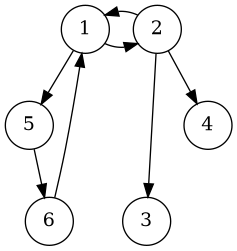
\includegraphics[width=0.2\linewidth,height=\textheight,keepaspectratio]{chapters/images/g7.png}

}

\caption{\label{fig-grafo7}Grafo direcionado}

\end{figure}%

Em um grafo direcionado, uma aresta é denominada \textbf{arco} e possui
uma origem e um destino. Um arco que parte de \(u\) e chega a \(v\) é
representado pelo par ordenado

\[
(u,v).
\]

Observe que, ao contrário dos pares não ordenados utilizados nos grafos
não direcionados,

\[
(u,v)\neq(v,u)
\]

em geral.

Formalmente, um grafo direcionado pode ser representado por

\[
G=(V,E),
\]

em que

\[
E\subseteq V\times V.
\]

Nesse caso, cada elemento de \(E\) é um par ordenado de vértices.

A direção dos arcos permite representar relações assimétricas. Por
exemplo, em uma rede de páginas da Web, uma página pode possuir um link
para outra sem que a segunda possua necessariamente um link de volta
para a primeira.

\subsection{Grau de entrada e grau de
saída}\label{grau-de-entrada-e-grau-de-sauxedda}

Em um grafo direcionado, é necessário distinguir as arestas que chegam a
um vértice daquelas que saem dele.

O \textbf{grau de entrada} de um vértice \(v\), representado por

\[
\deg^-(v),
\]

é o número de arcos que chegam a \(v\).

O \textbf{grau de saída}, representado por

\[
\deg^+(v),
\]

é o número de arcos que partem de \(v\).

Essa distinção é fundamental no estudo dos autômatos. Um estado pode
possuir várias transições de saída e várias transições de entrada. Em um
AFD, por exemplo, para cada estado e símbolo do alfabeto existe
exatamente uma transição correspondente.

\subsection{Caminhos direcionados}\label{caminhos-direcionados}

Em um grafo direcionado, um \textbf{caminho direcionado} é uma sequência
de vértices na qual cada arco é percorrido respeitando sua direção.

Considere, por exemplo, os arcos

\[
(a,b),\quad
(b,c),\quad
(c,d).
\]

Nesse caso,

\[
(a,b,c,d)
\]

é um caminho direcionado.

Entretanto, se o arco disponível for \((b,a)\) em vez de \((a,b)\), não
será possível percorrer esse arco de \(a\) para \(b\). Essa
característica diferencia fundamentalmente os caminhos em grafos
direcionados daqueles existentes em grafos não direcionados.

Em um autômato, o processamento de uma cadeia pode ser interpretado como
um caminho direcionado no grafo de estados. Cada símbolo lido determina
qual transição deve ser percorrida.

\subsection{Conectividade forte}\label{conectividade-forte}

Um grafo direcionado é \textbf{fortemente conexo} quando, para quaisquer
dois vértices \(u\) e \(v\), existe um caminho direcionado de \(u\) para
\(v\) e também um caminho direcionado de \(v\) para \(u\).

A conectividade forte é uma propriedade mais restritiva que a
conectividade de um grafo não direcionado, pois exige que os caminhos
possam ser percorridos respeitando as direções dos arcos.

As \textbf{componentes fortemente conexas} de um grafo direcionado são
subconjuntos máximos de vértices nos quais todos os vértices são
mutuamente alcançáveis por caminhos direcionados. Esse conceito possui
aplicações em análise de programas, redes, compiladores e algoritmos
sobre grafos.

\subsection{Grafos e relações}\label{grafos-e-relauxe7uxf5es}

Existe uma conexão direta entre grafos direcionados e relações binárias.
Seja \(D\) um conjunto e seja

\[
R\subseteq D\times D
\]

uma relação binária sobre \(D\).

Podemos construir um grafo direcionado

\[
G=(D,E),
\]

definindo

\[
E=\{(x,y)\mid xRy\}.
\]

Nesse grafo, cada elemento de \(D\) corresponde a um vértice e cada par
\((x,y)\) pertencente à relação corresponde a um arco de \(x\) para
\(y\).

Essa correspondência permite representar relações matemáticas
graficamente.

Por exemplo, considere a relação

\[
R=\{(x,y)\in\mathbb{Z}\times\mathbb{Z}\mid x<y\}.
\]

Podemos interpretar essa relação como um grafo direcionado em que existe
um arco de \(x\) para \(y\) sempre que \(x<y\).

Essa conexão entre relações e grafos é importante porque permite
utilizar propriedades gráficas para analisar relações matemáticas. Da
mesma forma, propriedades de relações, como reflexividade, simetria e
transitividade, podem ser interpretadas em termos da estrutura do grafo
correspondente.

\section{Lógica Booleana}\label{luxf3gica-booleana}

A \textbf{Lógica Booleana} é um sistema matemático utilizado para
representar e manipular informações que podem assumir dois valores
distintos. Esses valores são normalmente denominados \textbf{verdadeiro}
e \textbf{falso} e podem ser representados, respectivamente, pelos
valores \(1\) e \(0\).

A lógica booleana está presente em diversas áreas da Computação. Ela é
utilizada na construção de circuitos digitais, na representação de
condições em programas, na consulta a bancos de dados, na definição de
propriedades matemáticas e na descrição de decisões tomadas por sistemas
computacionais.

O conjunto de valores booleanos pode ser representado por

\[
\mathbb{B}=\{0,1\},
\]

em que \(0\) representa falso e \(1\) representa verdadeiro.

Uma expressão construída a partir de variáveis booleanas e operadores
lógicos é denominada \textbf{expressão booleana}. Por exemplo,

\[
P\wedge Q
\]

é uma expressão booleana formada pelas variáveis \(P\) e \(Q\) e pelo
operador de conjunção.

\subsection{Proposições}\label{proposiuxe7uxf5es}

Uma \textbf{proposição} é uma afirmação que pode ser classificada como
verdadeira ou falsa, mas não pode assumir simultaneamente os dois
valores.

Por exemplo, a afirmação

\begin{quote}
\(2+3=5\)
\end{quote}

é uma proposição verdadeira, enquanto

\begin{quote}
\(2+3=6\)
\end{quote}

é uma proposição falsa.

Podemos representar proposições por letras, como \(P\), \(Q\) e \(R\).
Assim, podemos escrever

\[
P=1
\]

para indicar que a proposição \(P\) é verdadeira, ou

\[
P=0
\]

para indicar que \(P\) é falsa.

É importante distinguir uma proposição de uma expressão que contém
variáveis não determinadas. Por exemplo,

\[
x>5
\]

não possui um valor lógico definido enquanto o valor de \(x\) não for
conhecido. Entretanto, uma vez determinado \(x\), a expressão poderá ser
avaliada como verdadeira ou falsa.

\subsection{Operações lógicas}\label{operauxe7uxf5es-luxf3gicas}

As proposições podem ser combinadas utilizando \textbf{operadores
lógicos}. Os operadores básicos são a negação, a conjunção e a
disjunção. Outros operadores, como o ou-exclusivo, a implicação e a
equivalência, podem ser definidos a partir desses operadores.

\subsubsection{Negação}\label{negauxe7uxe3o}

A \textbf{negação}, representada pelo símbolo \(\neg\), inverte o valor
lógico de uma proposição.

A tabela-verdade da negação é

\begin{longtable*}[]{|c|c|}
\toprule\noalign{}
\(P\) & \(\neg P\) \\
\midrule\noalign{}
\endhead
\bottomrule\noalign{}
\endlastfoot
\(0\) & \(1\) \\
\midrule
\(1\) & \(0\) \\
\end{longtable*}

Assim, se \(P\) é verdadeira, então \(\neg P\) é falsa. Da mesma forma,
se \(P\) é falsa, então \(\neg P\) é verdadeira.

Podemos representar a operação por

\[
\neg 0=1
\]

e

\[
\neg 1=0.
\]

\subsubsection{Conjunção}\label{conjunuxe7uxe3o}

A \textbf{conjunção}, representada por \(\wedge\), corresponde ao
operador lógico \textbf{E}. A expressão

\[
P\wedge Q
\]

é verdadeira somente quando \(P\) e \(Q\) são simultaneamente
verdadeiras.

Sua tabela-verdade é

\begin{longtable*}[]{|c|c|c|}
\toprule\noalign{}
\(P\) & \(Q\) & \(P\wedge Q\) \\
\midrule\noalign{}
\endhead
\bottomrule\noalign{}
\endlastfoot
\(0\) & \(0\) & \(0\) \\
\midrule
\(0\) & \(1\) & \(0\) \\
\midrule
\(1\) & \(0\) & \(0\) \\
\midrule
\(1\) & \(1\) & \(1\) \\
\end{longtable*}

Por exemplo, considere as proposições:

\[
P=\text{``10 é maior que 5''}
\]

e

\[
Q=\text{``10 é par''}.
\]

As duas proposições são verdadeiras. Portanto,

\[
P\wedge Q=1.
\]

A conjunção exige que todas as proposições envolvidas sejam verdadeiras.

\subsubsection{Disjunção}\label{disjunuxe7uxe3o}

A \textbf{disjunção}, representada por \(\vee\), corresponde ao operador
lógico \textbf{OU}. A expressão

\[
P\vee Q
\]

é verdadeira quando pelo menos uma das proposições é verdadeira.

Sua tabela-verdade é

\begin{longtable*}[]{|c|c|c|}
\toprule\noalign{}
\(P\) & \(Q\) & \(P\vee Q\) \\
\midrule\noalign{}
\endhead
\bottomrule\noalign{}
\endlastfoot
\(0\) & \(0\) & \(0\) \\
\midrule
\(0\) & \(1\) & \(1\) \\
\midrule
\(1\) & \(0\) & \(1\) \\
\midrule
\(1\) & \(1\) & \(1\) \\
\end{longtable*}

Portanto,

\[
0\vee0=0,
\]

enquanto

\[
0\vee1=1,
\]

\[
1\vee0=1
\]

e

\[
1\vee1=1.
\]

Na lógica booleana, o operador \(\vee\) corresponde ao \textbf{OU
inclusivo}, pois o resultado também é verdadeiro quando ambas as
proposições são verdadeiras.

\subsubsection{Ou-exclusivo}\label{ou-exclusivo}

O \textbf{ou-exclusivo}, representado por \(\oplus\), é verdadeiro
quando exatamente uma das duas proposições é verdadeira.

Sua tabela-verdade é

\begin{longtable*}[]{|c|c|c|}
\toprule\noalign{}
\(P\) & \(Q\) & \(P\oplus Q\) \\
\midrule\noalign{}
\endhead
\bottomrule\noalign{}
\endlastfoot
\(0\) & \(0\) & \(0\) \\
\midrule
\(0\) & \(1\) & \(1\) \\
\midrule
\(1\) & \(0\) & \(1\) \\
\midrule
\(1\) & \(1\) & \(0\) \\
\end{longtable*}

Assim,

\[
P\oplus Q
\]

é verdadeiro quando \(P\) e \(Q\) possuem valores diferentes.

Uma forma de expressar o ou-exclusivo utilizando outros operadores é

\[
P\oplus Q
\equiv
(P\vee Q)\wedge\neg(P\wedge Q).
\]

Outra representação equivalente é

\[
P\oplus Q
\equiv
\neg(P\leftrightarrow Q).
\]

\subsubsection{Implicação}\label{implicauxe7uxe3o}

A \textbf{implicação}, representada por \(\rightarrow\), é utilizada
para expressar uma condição do tipo ``se\ldots{} então\ldots{}''.

A expressão

\[
P\rightarrow Q
\]

é lida como:

\begin{quote}
Se \(P\), então \(Q\).
\end{quote}

Sua tabela-verdade é

\begin{longtable*}[]{|c|c|c|}
\toprule\noalign{}
\(P\) & \(Q\) & \(P\rightarrow Q\) \\
\midrule\noalign{}
\endhead
\bottomrule\noalign{}
\endlastfoot
\(0\) & \(0\) & \(1\) \\
\midrule
\(0\) & \(1\) & \(1\) \\
\midrule
\(1\) & \(0\) & \(0\) \\
\midrule
\(1\) & \(1\) & \(1\) \\
\end{longtable*}

Observe que a implicação é falsa somente quando \(P\) é verdadeira e
\(Q\) é falsa.

Uma propriedade importante é que a implicação pode ser expressa
utilizando apenas a negação e a disjunção:

\[
P\rightarrow Q
\equiv
\neg P\vee Q.
\]

Também pode ser expressa utilizando apenas a negação e a conjunção:

\[
P\rightarrow Q
\equiv
\neg(P\wedge\neg Q).
\]

Essa equivalência é útil porque mostra que a implicação não precisa
necessariamente ser considerada um operador lógico básico.

\subsubsection{Equivalência lógica}\label{equivaluxeancia-luxf3gica}

A \textbf{equivalência lógica}, representada por \(\leftrightarrow\),
estabelece que duas proposições possuem o mesmo valor lógico.

A expressão

\[
P\leftrightarrow Q
\]

é verdadeira quando \(P\) e \(Q\) possuem o mesmo valor.

Sua tabela-verdade é

\begin{longtable*}[]{|c|c|c|}
\toprule\noalign{}
\(P\) & \(Q\) & \(P\leftrightarrow Q\) \\
\midrule\noalign{}
\endhead
\bottomrule\noalign{}
\endlastfoot
\(0\) & \(0\) & \(1\) \\
\midrule
\(0\) & \(1\) & \(0\) \\
\midrule
\(1\) & \(0\) & \(0\) \\
\midrule
\(1\) & \(1\) & \(1\) \\
\end{longtable*}

A equivalência lógica pode ser expressa por duas implicações:

\[
P\leftrightarrow Q
\equiv
(P\rightarrow Q)\wedge(Q\rightarrow P).
\]

Também podemos escrevê-la como

\[
P\leftrightarrow Q
\equiv
(P\wedge Q)\vee(\neg P\wedge\neg Q).
\]

Essa última expressão evidencia que \(P\leftrightarrow Q\) é verdadeira
quando ambas são verdadeiras ou quando ambas são falsas.

\subsection{Expressões booleanas}\label{expressuxf5es-booleanas}

Operadores lógicos podem ser combinados para formar expressões mais
complexas. Por exemplo,

\[
(P\wedge Q)\vee\neg R
\]

é uma expressão booleana formada pelas variáveis \(P\), \(Q\) e \(R\).

O valor da expressão depende dos valores atribuídos às variáveis. Para
determinar o resultado de uma expressão, podemos construir uma
\textbf{tabela-verdade} contendo todas as combinações possíveis de
valores das variáveis.

Se uma expressão possui \(n\) variáveis booleanas, existem

\[
2^n
\]

possíveis combinações de valores.

Por exemplo, uma expressão com três variáveis \(P\), \(Q\) e \(R\)
possui

\[
2^3=8
\]

combinações possíveis.

Uma tabela-verdade completa permite determinar o resultado de uma
expressão para cada uma dessas combinações.

\subsection{Tabelas-verdade}\label{tabelas-verdade}

Considere a expressão

\[
P\wedge(Q\vee R).
\]

Para construir sua tabela-verdade, começamos listando todas as
combinações possíveis de \(P\), \(Q\) e \(R\):

\begin{longtable*}[]{|c|c|c|c|c|}
\toprule\noalign{}
\(P\) & \(Q\) & \(R\) & \(Q\vee R\) & \(P\wedge(Q\vee R)\) \\
\midrule\noalign{}
\endhead
\bottomrule\noalign{}
\endlastfoot
0 & 0 & 0 & 0 & 0 \\
\midrule
0 & 0 & 1 & 1 & 0 \\
\midrule
0 & 1 & 0 & 1 & 0 \\
\midrule
0 & 1 & 1 & 1 & 0 \\
\midrule
1 & 0 & 0 & 0 & 0 \\
\midrule
1 & 0 & 1 & 1 & 1 \\
\midrule
1 & 1 & 0 & 1 & 1 \\
\midrule
1 & 1 & 1 & 1 & 1 \\
\end{longtable*}

A tabela-verdade permite verificar propriedades das expressões booleanas
de maneira sistemática.

Ela também fornece um método para verificar se duas expressões são
logicamente equivalentes. Basta construir as respectivas tabelas-verdade
e comparar suas colunas finais.

\subsection{Tautologias e
contradições}\label{tautologias-e-contradiuxe7uxf5es}

Uma expressão booleana é uma \textbf{tautologia} quando seu resultado é
verdadeiro para todas as possíveis atribuições de valores às suas
variáveis.

Um exemplo é

\[
P\vee\neg P.
\]

Independentemente do valor de \(P\), uma das duas partes será
verdadeira. Portanto,

\[
P\vee\neg P\equiv1.
\]

Uma expressão é uma \textbf{contradição} quando seu resultado é falso
para todas as possíveis atribuições.

Um exemplo é

\[
P\wedge\neg P.
\]

Nesse caso,

\[
P\wedge\neg P\equiv0.
\]

Também podemos ter expressões que são verdadeiras para algumas
atribuições e falsas para outras. Essas expressões são denominadas
\textbf{contingências}.

Portanto, uma expressão booleana pode ser classificada, de acordo com
seu comportamento, como tautologia, contradição ou contingência.

\subsection{Equivalências booleanas}\label{equivaluxeancias-booleanas}

Duas expressões booleanas são \textbf{logicamente equivalentes} quando
produzem o mesmo resultado para todas as possíveis atribuições de
valores às suas variáveis.

Podemos representar essa equivalência por

\[
P\equiv Q.
\]

Por exemplo,

\[
P\rightarrow Q
\equiv
\neg P\vee Q.
\]

As duas expressões possuem o mesmo valor para todas as combinações de
\(P\) e \(Q\).

As equivalências lógicas permitem transformar expressões sem alterar seu
significado lógico. Essa propriedade é muito útil para simplificar
expressões e demonstrar propriedades de sistemas que utilizam lógica
booleana.

\subsection{Leis de De Morgan}\label{leis-de-de-morgan}

Entre as equivalências mais importantes da lógica booleana estão as
\textbf{Leis de De Morgan}:

\[
\neg(P\wedge Q)
\equiv
\neg P\vee\neg Q
\]

e

\[
\neg(P\vee Q)
\equiv
\neg P\wedge\neg Q.
\]

A primeira afirma que negar uma conjunção equivale a realizar a
disjunção das negações. A segunda afirma que negar uma disjunção
equivale a realizar a conjunção das negações.

Essas leis podem ser verificadas diretamente por meio de
tabelas-verdade.

Por exemplo:

\begin{longtable*}[]{|c|c|c|c|}
\toprule\noalign{}
\(P\) & \(Q\) & \(\neg(P\wedge Q)\) & \(\neg P\vee\neg Q\) \\
\midrule\noalign{}
\endhead
\bottomrule\noalign{}
\endlastfoot
0 & 0 & 1 & 1 \\
\midrule
0 & 1 & 1 & 1 \\
\midrule
1 & 0 & 1 & 1 \\
\midrule
1 & 1 & 0 & 0 \\
\end{longtable*}

As duas últimas colunas são iguais, confirmando a equivalência.

\subsection{Leis distributivas}\label{leis-distributivas}

A lógica booleana possui também leis distributivas. Para a conjunção e a
disjunção temos

\[
P\wedge(Q\vee R)
\equiv
(P\wedge Q)\vee(P\wedge R)
\]

e

\[
P\vee(Q\wedge R)
\equiv
(P\vee Q)\wedge(P\vee R).
\]

Essas expressões possuem uma estrutura semelhante às leis distributivas
conhecidas da aritmética. Entretanto, é importante observar que a
álgebra booleana não é simplesmente a aritmética com os valores \(0\) e
\(1\).

Na aritmética usual,

\[
a(b+c)=ab+ac,
\]

enquanto na lógica booleana os operadores envolvidos são \(\wedge\) e
\(\vee\).

A existência das duas leis distributivas é uma das diferenças
interessantes entre a álgebra booleana e a álgebra aritmética
tradicional.

\subsection{Outras leis importantes}\label{outras-leis-importantes}

Diversas outras equivalências podem ser utilizadas para manipular
expressões booleanas. Entre elas estão as leis de identidade:

\[
P\wedge1\equiv P
\]

e

\[
P\vee0\equiv P.
\]

As leis de dominação são

\[
P\vee1\equiv1
\]

e

\[
P\wedge0\equiv0.
\]

As leis de idempotência são

\[
P\vee P\equiv P
\]

e

\[
P\wedge P\equiv P.
\]

As leis de complemento são

\[
P\vee\neg P\equiv1
\]

e

\[
P\wedge\neg P\equiv0.
\]

Também temos as leis de dupla negação:

\[
\neg(\neg P)\equiv P.
\]

Essas leis fornecem regras para transformar e simplificar expressões
booleanas.

\subsection{Conjuntos completos de
operadores}\label{conjuntos-completos-de-operadores}

Embora vários operadores possam ser utilizados na construção de
expressões booleanas, nem todos são necessários. Um conjunto de
operadores é denominado \textbf{completo} quando qualquer função
booleana pode ser expressa utilizando apenas os operadores desse
conjunto.

Por exemplo, \({\neg,\wedge}\) é um conjunto completo. A partir da
negação e da conjunção podemos representar a disjunção utilizando a Lei
de De Morgan:

\[
P\vee Q
\equiv
\neg(\neg P\wedge\neg Q).
\]

A implicação pode então ser representada por

\[
P\rightarrow Q
\equiv
\neg(P\wedge\neg Q).
\]

A equivalência pode ser construída como

\[
P\leftrightarrow Q
\equiv
\neg(P\wedge\neg Q)
\wedge
\neg(Q\wedge\neg P).
\]

E o ou-exclusivo pode ser representado por

\[
P\oplus Q
\equiv
\neg\left(
\neg(P\wedge\neg Q)
\wedge
\neg(Q\wedge\neg P)
\right).
\]

Dessa maneira, operações que inicialmente parecem diferentes podem ser
construídas a partir de um conjunto menor de operações básicas.

Outro exemplo importante é o operador \textbf{NAND}, definido por

\[
P\uparrow Q=\neg(P\wedge Q).
\]

O operador NAND, isoladamente, também forma um conjunto completo. Isso
significa que qualquer função booleana pode ser construída utilizando
exclusivamente operadores NAND. Essa propriedade possui aplicações
importantes na construção de circuitos digitais.

\subsection{Álgebra Booleana}\label{uxe1lgebra-booleana}

A lógica booleana pode ser estudada também por meio de uma estrutura
algébrica. As operações \(\wedge\), \(\vee\) e \(\neg\), juntamente com
os valores \(0\) e \(1\), obedecem a um conjunto de leis que permite
manipular expressões formalmente.

Essa estrutura é denominada \textbf{álgebra booleana}.

Uma maneira de visualizar a correspondência entre a lógica e a álgebra é
observar que:

\begin{longtable*}[]{|l|l|}
\toprule\noalign{}
Lógica & Álgebra Booleana \\
\midrule\noalign{}
\endhead
\bottomrule\noalign{}
\endlastfoot
verdadeiro & \(1\) \\
\midrule
falso & \(0\) \\
\midrule
E & \(\wedge\) \\
\midrule
OU & \(\vee\) \\
\midrule
NÃO & \(\neg\) \\
\end{longtable*}

Essa correspondência permite utilizar técnicas algébricas para
transformar expressões lógicas.

É importante, entretanto, lembrar que os símbolos \(\wedge\) e \(\vee\)
representam operações específicas e não devem ser confundidos
diretamente com a multiplicação e a adição convencionais. Embora existam
algumas semelhanças formais, as estruturas matemáticas possuem
propriedades próprias.

\subsection{Síntese}\label{suxedntese}

A lógica booleana fornece uma linguagem matemática para representar
informações que possuem dois valores possíveis. Seus valores básicos são

\[
\mathbb{B}=\{0,1\},
\]

em que \(0\) representa falso e \(1\) representa verdadeiro.

As operações fundamentais são a negação, a conjunção e a disjunção:

\[
\neg,\qquad
\wedge,\qquad
\vee.
\]

A partir delas podem ser definidos outros operadores, como o
ou-exclusivo, a implicação e a equivalência:

\[
\oplus,\qquad
\rightarrow,\qquad
\leftrightarrow.
\]

As operações podem ser combinadas para formar expressões booleanas, cujo
comportamento pode ser analisado por meio de tabelas-verdade. Uma
expressão pode ser uma tautologia, uma contradição ou uma contingência,
dependendo de seu comportamento para as diferentes atribuições de
valores às variáveis.

As equivalências lógicas permitem transformar expressões sem modificar
seus resultados. Entre as propriedades mais importantes estão as Leis de
De Morgan, as leis distributivas, as leis de identidade, dominação,
idempotência, complemento e dupla negação.

A lógica booleana pode ser resumida como um sistema em que valores,
operações e propriedades são combinados para produzir e manipular
expressões formais:

\[
\boxed{
\text{valores}
\longrightarrow
\text{operações}
\longrightarrow
\text{expressões}
\longrightarrow
\text{tabelas-verdade}
\longrightarrow
\text{equivalências}
}
\]

Esses conceitos fornecem uma base matemática para o tratamento formal de
condições, decisões e propriedades booleanas e serão utilizados como
ferramentas fundamentais em diferentes áreas da Computação.

\section{Definições, Teoremas e
Provas}\label{definiuxe7uxf5es-teoremas-e-provas}

A Matemática é construída a partir de conceitos, propriedades e
argumentos que permitem estabelecer relações entre esses conceitos. Para
apresentar esses resultados de maneira precisa, utilizamos
principalmente \textbf{definições}, \textbf{enunciados matemáticos} e
\textbf{provas}. Esses elementos também são fundamentais no estudo de
estruturas matemáticas utilizadas na Computação.

Uma definição estabelece exatamente o significado de um conceito. Um
enunciado afirma que determinada propriedade é verdadeira. Uma prova
fornece uma justificativa matemática para essa afirmação. Quando um
enunciado é demonstrado, ele pode receber diferentes denominações, como
proposição, lema, teorema ou corolário, dependendo principalmente de sua
função dentro do desenvolvimento matemático.

\subsection{Definições}\label{definiuxe7uxf5es}

Uma \textbf{definição} estabelece formalmente o significado de um
objeto, propriedade ou conceito matemático. Ela não é uma afirmação que
precisa ser demonstrada como verdadeira ou falsa; seu objetivo é
estabelecer uma convenção precisa que será utilizada posteriormente.

Por exemplo, podemos definir uma cadeia como uma sequência finita de
símbolos pertencentes a um alfabeto. A partir dessa definição, podemos
utilizar o conceito de cadeia em outras definições e resultados.

Da mesma forma, podemos definir um grafo simples como um grafo que não
possui laços nem arestas múltiplas. Depois que essa definição foi
estabelecida, podemos utilizá-la em teoremas e provas envolvendo grafos.

As definições são particularmente importantes porque eliminam
ambiguidades. Em uma disciplina formal, termos como cadeia, linguagem,
autômato, árvore ou grafo precisam possuir um significado preciso para
que seja possível argumentar matematicamente sobre eles.

Uma definição também pode utilizar conceitos que já foram definidos
anteriormente. Dessa maneira, o conhecimento matemático é construído de
forma incremental: novos conceitos são definidos a partir de conceitos
previamente estabelecidos.

\subsection{Enunciados matemáticos}\label{enunciados-matemuxe1ticos}

Um \textbf{enunciado matemático} é uma afirmação que pode ser analisada
quanto à sua validade. Dependendo do contexto, um enunciado pode ser
denominado proposição, lema, teorema ou corolário.

Por exemplo:

\begin{quote}
Todo número inteiro par é divisível por 2.
\end{quote}

é um enunciado matemático. Podemos investigar sua validade e construir
uma demonstração.

Em geral, um enunciado pode possuir uma estrutura lógica. Uma forma
bastante comum é a implicação

\[
P\rightarrow Q,
\]

que pode ser interpretada como ``se \(P\) é verdadeira, então \(Q\)
também é verdadeira''.

Por exemplo:

\[
n\text{ é divisível por }4
\rightarrow
n\text{ é par}.
\]

Nesse caso, a hipótese é que \(n\) seja divisível por \(4\) e a
conclusão é que \(n\) seja par.

A identificação da hipótese e da conclusão é importante porque muitos
métodos de demonstração dependem diretamente da estrutura lógica do
enunciado.

\subsection{Provas}\label{provas}

Uma \textbf{prova matemática} é uma sequência de argumentos que
estabelece a validade de um enunciado a partir de definições,
propriedades já demonstradas, axiomas e regras de inferência.

Uma prova não deve apenas apresentar exemplos que confirmem uma
afirmação. Para demonstrar uma propriedade geral, é necessário mostrar
que ela é válida para todos os objetos que satisfazem as condições
estabelecidas.

Por exemplo, considere o enunciado:

\[
\text{Para todo }n\in\mathbb{Z},\quad
n\text{ par}\Rightarrow n^2\text{ par}.
\]

Podemos verificar que isso acontece para alguns valores:

\[
2^2=4,
\qquad
4^2=16,
\qquad
6^2=36.
\]

Entretanto, esses exemplos não constituem uma prova. Eles apenas
fornecem evidências para a afirmação. Uma prova precisa considerar um
número par arbitrário.

Se \(n\) é par, pela definição de número par existe um inteiro \(k\) tal
que

\[
n=2k.
\]

Então,

\[
n^2=(2k)^2=4k^2=2(2k^2).
\]

Como \(2k^2\) é um inteiro, concluímos que \(n^2\) é par.

Essa demonstração vale para qualquer número inteiro par e, portanto,
estabelece o resultado.

\subsection{Teoremas, lemas e
corolários}\label{teoremas-lemas-e-coroluxe1rios}

Um \textbf{teorema} é um enunciado matemático que foi demonstrado
formalmente. Os teoremas normalmente representam resultados importantes
dentro de uma teoria.

Um \textbf{lema} também é um enunciado demonstrado, mas geralmente é
utilizado como uma ferramenta auxiliar para demonstrar outro resultado
mais importante. Um lema não é necessariamente menos difícil ou menos
importante que um teorema; sua denominação está relacionada
principalmente à função que desempenha na construção da teoria.

Um \textbf{corolário} é um resultado que pode ser obtido diretamente a
partir de um teorema ou de um resultado já demonstrado. Em geral, sua
demonstração é mais simples porque depende de um resultado anterior.

Por exemplo, uma teoria pode seguir uma estrutura como

\[
\text{Definições}
\rightarrow
\text{Lemas}
\rightarrow
\text{Teorema}
\rightarrow
\text{Corolários}.
\]

Essa organização permite construir resultados complexos a partir de
resultados mais elementares.

\subsection{Conjecturas}\label{conjecturas}

Uma \textbf{conjectura} é um enunciado para o qual existem evidências ou
argumentos que sugerem sua validade, mas que ainda não possui uma
demonstração matemática aceita.

Uma conjectura pode posteriormente ser demonstrada, tornando-se um
teorema, ou pode ser refutada pela apresentação de um contraexemplo.

É importante distinguir uma conjectura de um teorema. Mesmo que uma
afirmação tenha sido verificada para muitos casos, isso não significa
que ela tenha sido demonstrada para todos os casos.

Por exemplo, suponha que uma propriedade tenha sido verificada para os
primeiros milhares de valores de uma variável. Isso fornece uma
evidência experimental, mas não constitui, por si só, uma prova
matemática.

Um único contraexemplo é suficiente para mostrar que um enunciado
universal é falso. Se uma afirmação possui a forma

\[
\forall x\in A,\quad P(x),
\]

basta encontrar um elemento \(x\in A\) para o qual

\[
P(x)
\]

seja falsa para refutar a afirmação.

\subsection{Prova direta}\label{prova-direta}

A \textbf{prova direta} é uma das formas mais simples de demonstração.
Nesse método, partimos das hipóteses do enunciado e aplicamos
definições, propriedades e resultados já conhecidos até chegar à
conclusão desejada.

Considere o seguinte resultado.

\textbf{Teorema:} Se \(n\) é um número inteiro par, então \(n^2\) é par.

Como vimos anteriormente, se \(n\) é par, então existe um inteiro \(k\)
tal que

\[
n=2k.
\]

Elevando ambos os lados ao quadrado,

\[
n^2=(2k)^2=4k^2.
\]

Podemos escrever

\[
n^2=2(2k^2).
\]

Como \(2k^2\) é inteiro, concluímos que \(n^2\) é par.

Nesse exemplo, partimos diretamente da hipótese e construímos uma
sequência de passos que conduz à conclusão.

A estrutura geral de uma prova direta de um enunciado

\[
P\rightarrow Q
\]

é:

\[
P
\rightarrow
P_1
\rightarrow
P_2
\rightarrow
\cdots
\rightarrow
Q.
\]

\subsection{Prova por construção}\label{prova-por-construuxe7uxe3o}

Em uma prova por construção, demonstramos a existência de um objeto
apresentando explicitamente uma forma de construí-lo.

Esse método é particularmente útil quando o enunciado afirma que
determinado objeto existe.

Considere o seguinte resultado sobre grafos.

Teorema: Para todo número par \(n>2\), existe um grafo 3-regular com
\(n\) vértices.

Um grafo é denominado 3-regular quando todos os seus vértices possuem
grau \(3\).

Para demonstrar o resultado, podemos construir explicitamente o grafo.
Seja

\[
n>2
\]

um número par e considere os vértices

\[
V={0,1,\ldots,n-1}.
\]

Inicialmente, conectamos os vértices formando um ciclo:

\[
0-1-2-\cdots-(n-1)-0.
\]

Cada vértice possui, nesse momento, grau \(2\).

Como \(n\) é par, podemos então adicionar uma aresta entre cada vértice
da primeira metade e o vértice correspondente da segunda metade. Para

\[
0\leq i<\frac n2,
\]

adicionamos a aresta

\[
{i,i+n/2}.
\]

Cada vértice recebe exatamente uma nova aresta. Portanto, todos os
vértices passam a possuir grau

\[
2+1=3.
\]

O grafo construído é, consequentemente, 3-regular e possui \(n\)
vértices.

O aspecto fundamental dessa prova é que não nos limitamos a afirmar que
o grafo existe. Nós apresentamos um procedimento que permite construí-lo
para qualquer número par \(n>2\).

A prova por construção é bastante comum em Computação. Muitos algoritmos
podem ser interpretados como construções que demonstram a existência de
uma solução ao mesmo tempo em que fornecem um procedimento para obtê-la.

\subsection{Prova por contradição}\label{prova-por-contradiuxe7uxe3o}

Na prova por contradição, assumimos inicialmente que o enunciado que
queremos demonstrar é falso. Em seguida, mostramos que essa hipótese
conduz a uma contradição.

Considere o conhecido resultado:

Teorema: \(\sqrt{2}\) é irracional.

Para demonstrá-lo, suponha, por contradição, que \(\sqrt{2}\) seja
racional. Nesse caso, podemos escrever

\[
\sqrt{2}=\frac{m}{n},
\]

em que \(m\) e \(n\) são inteiros, \(n\neq0\), e a fração está na forma
irredutível.

Elevando ambos os lados ao quadrado,

\[
2=\frac{m^2}{n^2}.
\]

Portanto,

\[
m^2=2n^2.
\]

Isso significa que \(m^2\) é par e, consequentemente, \(m\) também é
par. Podemos escrever

\[
m=2k
\]

para algum inteiro \(k\).

Substituindo na equação anterior,

\[
(2k)^2=2n^2.
\]

Logo,

\[
4k^2=2n^2
\]

e, dividindo por \(2\),

\[
n^2=2k^2.
\]

Portanto, \(n^2\) também é par e, consequentemente, \(n\) é par.

Chegamos então à conclusão de que tanto \(m\) quanto \(n\) são pares.
Isso significa que ambos possuem o fator \(2\), contradizendo a hipótese
de que \(\frac{m}{n}\) estava na forma irredutível.

A hipótese de que \(\sqrt{2}\) é racional levou a uma contradição.
Portanto,

\[
\boxed{\sqrt{2}\text{ é irracional}.}
\]

A estrutura geral de uma prova por contradição pode ser representada por

\[
\neg P
\rightarrow
\text{contradição}.
\]

Consequentemente, concluímos que

\[
P.
\]

Esse método é particularmente útil quando a negação do resultado possui
uma estrutura mais fácil de analisar do que o próprio resultado.

\subsection{Prova por indução
matemática}\label{prova-por-induuxe7uxe3o-matemuxe1tica}

A indução matemática é um método utilizado para demonstrar propriedades
que dependem de números naturais.

A ideia fundamental é semelhante à de uma sequência de dominós. Primeiro
demonstramos que a propriedade é verdadeira para o primeiro caso. Depois
mostramos que, sempre que ela for verdadeira para um determinado caso,
também será verdadeira para o caso seguinte. Dessa forma, a propriedade
vale para todos os casos a partir do primeiro.

Considere o teorema:

Teorema: \[
\sum_{i = 0}^n i = 
\frac{n(n+1)}{2},
\qquad n\geq0.
\]

A demonstração possui duas etapas principais: o passo base e o passo
indutivo.

Passo base

Verificamos inicialmente o caso \(n=0\):

\[
\sum_{i=0}^{0}i=0.
\]

A fórmula fornece

\[
\frac{0(0+1)}{2}=0.
\]

Portanto, a propriedade é verdadeira para \(n=0\).

Hipótese de indução

Agora assumimos que a propriedade é verdadeira para um número natural
arbitrário \(n\). Ou seja, assumimos que \[
\sum_{i = 0}^n i = 
\frac{n(n+1)}{2}.
\]

Essa afirmação é denominada hipótese de indução.

É importante observar que, nesse ponto, não estamos assumindo aquilo que
queremos provar para todos os valores. Estamos assumindo a propriedade
para um valor arbitrário \(n\) com o objetivo de demonstrá-la para
\(n+1\).

\subsubsection{Passo indutivo}\label{passo-indutivo}

Queremos demonstrar que \[
\sum_{i = 0}^{n + 1}  i = 
\frac{(n+1)(n+2)}{2}.
\]

Começamos pela soma: \[
\sum_{i = 0}^{n + 1}  i = 
\sum_{i=0}^{n}i+(n+1).
\]

Aplicando a hipótese de indução,

\[
\sum_{i = 0}^{n + 1} i = 
\frac{n(n+1)}{2}+(n+1).
\]

Colocando \((n+1)\) em evidência,

\[
\sum_{i = 0}^{n + 1} i = 
(n+1)
\left(
\frac n2+1
\right).
\]

Portanto,

\[
\sum_{i = 0}^{n + 1} i = 
(n+1)
\frac{n+2}{2}.
\]

Logo,

\[
\sum_{i = 0}^{n + 1} i = 
\frac{(n+1)(n+2)}{2}.
\]

Assim, mostramos que, se a propriedade é verdadeira para \(n\), ela
também é verdadeira para \(n+1\).

Como a propriedade é verdadeira para \(n=0\) e o passo indutivo é
válido, concluímos que

\[
\sum_{i = 0}^n i = 
\frac{n(n+1)}{2}.
\]

para todo \(n\geq0\).

\subsubsection{Estrutura da indução}\label{estrutura-da-induuxe7uxe3o}

O princípio da indução pode ser resumido da seguinte maneira:

\[
P(0)
\]

e

\[
\forall n\geq0,\quad
P(n)\rightarrow P(n+1).
\]

Então,

\[
\forall n\geq0,\quad P(n).
\]

A indução matemática é especialmente importante em Computação porque
muitas propriedades de algoritmos e estruturas de dados dependem do
tamanho de uma entrada. Também é comum utilizar indução para demonstrar
propriedades de cadeias, árvores, grafos, gramáticas e estruturas
recursivamente definidas.

\subsubsection{Indução forte}\label{induuxe7uxe3o-forte}

Existe uma variante denominada indução forte. Nesse caso, para
demonstrar \(P(n+1)\), podemos assumir que a propriedade é verdadeira
para todos os valores anteriores:

\[
P(0),P(1),\ldots,P(n).
\]

A hipótese de indução forte é, portanto,

\[
\forall k\leq n,\quad P(k).
\]

A partir dessa hipótese, demonstramos

\[
P(n+1).
\]

A indução forte é útil quando o caso seguinte depende de mais de um caso
anterior. Embora possua uma hipótese mais abrangente, ela é logicamente
equivalente ao princípio usual da indução matemática.

\subsection{Escolha do método de
prova}\label{escolha-do-muxe9todo-de-prova}

Diferentes enunciados podem exigir diferentes estratégias de
demonstração. Não existe um único método que seja adequado para todos os
problemas.

Se o objetivo é demonstrar que determinado objeto existe e podemos
apresentar explicitamente esse objeto, uma prova por construção pode ser
apropriada.

Quando a negação do resultado leva naturalmente a uma situação
impossível, podemos utilizar uma prova por contradição.

Quando o enunciado envolve uma sequência de casos indexados por números
naturais, a indução matemática frequentemente fornece uma estratégia
natural.

A prova direta é particularmente adequada quando podemos partir das
hipóteses e chegar à conclusão por uma sequência simples de implicações.

Em problemas mais complexos, diferentes métodos podem ser combinados.
Uma prova pode, por exemplo, utilizar indução e, dentro de cada etapa,
empregar uma prova por construção.

\subsection{Provas e contraexemplos}\label{provas-e-contraexemplos}

Uma maneira importante de analisar uma afirmação é procurar um
contraexemplo.

Um contraexemplo é um objeto que satisfaz as condições da hipótese de um
enunciado, mas não satisfaz sua conclusão.

Considere a afirmação:

Todo número primo é ímpar.

O número \(2\) é primo e é par. Portanto, \(2\) é um contraexemplo e
demonstra que a afirmação é falsa.

Um único contraexemplo é suficiente para refutar um enunciado universal.
Entretanto, a ausência de contraexemplos em um conjunto finito de testes
não constitui uma prova.

Essa distinção é especialmente importante em Computação. Um programa
pode ser executado com milhares ou milhões de entradas e produzir os
resultados esperados em todos os testes realizados. Isso não demonstra
necessariamente que o programa esteja correto para todas as entradas
possíveis.

Testes computacionais são ferramentas importantes para encontrar erros e
formular conjecturas, mas uma prova matemática possui um papel
diferente: estabelecer formalmente a validade de uma propriedade dentro
das condições consideradas.

\subsection{A estrutura de uma
demonstração}\label{a-estrutura-de-uma-demonstrauxe7uxe3o}

Uma demonstração matemática deve ser suficientemente clara para que seus
passos possam ser verificados.

Em geral, uma prova pode seguir a seguinte estrutura:

\begin{itemize}
\tightlist
\item
  Identificação das hipóteses: determinar quais condições são assumidas.
\item
  Definição dos objetos: utilizar corretamente as definições relevantes.
\item
  Aplicação de resultados conhecidos: utilizar propriedades, lemas e
  teoremas já demonstrados.
\item
  Desenvolvimento do argumento: estabelecer uma sequência lógica de
  passos.
\item
  Conclusão: mostrar explicitamente que o resultado desejado foi obtido.
\end{itemize}

É importante não utilizar como hipótese aquilo que deveria ser
demonstrado. Esse erro é conhecido como raciocínio circular.

Também é importante verificar se cada passo da prova realmente decorre
das informações anteriores. Uma prova matemática não é apenas uma
sequência de equações; cada transformação precisa ser justificada pelas
propriedades matemáticas disponíveis.

Definições, teoremas e provas em uma teoria matemática

Uma teoria matemática pode ser construída como uma sequência organizada
de definições e resultados.

Inicialmente, alguns conceitos são definidos. Em seguida, propriedades
desses conceitos são estabelecidas por meio de proposições e lemas.
Resultados mais importantes podem então ser demonstrados utilizando os
resultados anteriores.

Podemos representar esse processo como

\[
\boxed{
\text{Definições}
\rightarrow
\text{Proposições}
\rightarrow
\text{Lemas}
\rightarrow
\text{Teoremas}
\rightarrow
\text{Corolários}
}
\]

As provas estabelecem as conexões lógicas entre esses resultados.

Essa organização permite construir conhecimentos mais complexos sem que
seja necessário demonstrar novamente todos os resultados utilizados. Um
teorema pode depender de vários lemas, que por sua vez dependem de
definições e resultados ainda mais básicos.

\subsection{Síntese}\label{suxedntese-1}

Definições, enunciados e provas constituem elementos fundamentais da
construção matemática. As definições estabelecem o significado preciso
dos conceitos; os enunciados apresentam propriedades que podem ser
analisadas; e as provas fornecem argumentos formais que estabelecem a
validade dessas propriedades.

Os resultados demonstrados podem desempenhar diferentes papéis. Um
teorema apresenta um resultado matemático relevante, um lema normalmente
auxilia na demonstração de outros resultados e um corolário é obtido
diretamente de um resultado já demonstrado. Uma conjectura, por sua vez,
é uma afirmação que ainda não possui uma demonstração estabelecida.

Entre os principais métodos de demonstração estão a prova direta, a
prova por construção, a prova por contradição e a prova por indução
matemática. Cada método explora uma estratégia diferente para
estabelecer a validade de um enunciado.

Podemos resumir as principais ideias da seção da seguinte maneira:

\[
\boxed{
\begin{array}{c}
\text{Definições}\
\downarrow\
\text{Enunciados}\
\downarrow\
\text{Provas}\
\downarrow\
\text{Resultados demonstrados}
\end{array}}
\]

e, no caso das principais estratégias de demonstração,

\[
\boxed{
\text{Direta}
\qquad
\text{Construção}
\qquad
\text{Contradição}
\qquad
\text{Indução}
}
\]

O domínio dessas técnicas é essencial para o desenvolvimento de
argumentos rigorosos. Ao longo do estudo de estruturas matemáticas e
computacionais, as provas serão utilizadas para estabelecer propriedades
de cadeias, linguagens, autômatos, gramáticas, grafos e algoritmos.

\bookmarksetup{startatroot}

\chapter{As Linguagens Regulares e a Analise
Léxica}\label{as-linguagens-regulares-e-a-analise-luxe9xica}

\begin{center}
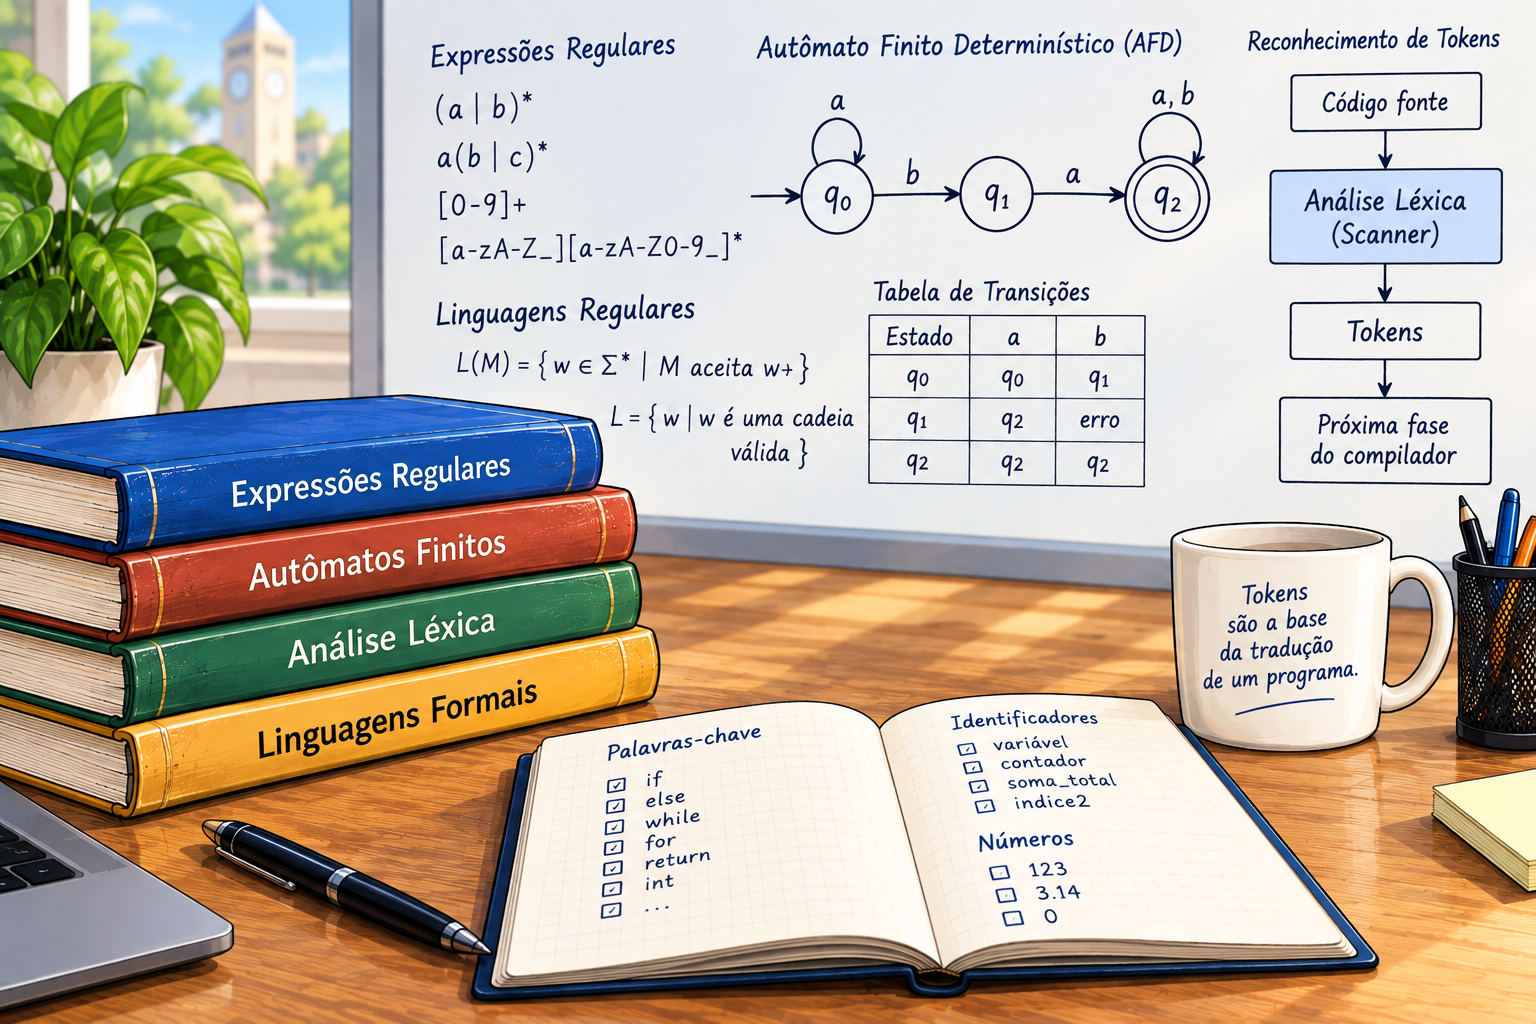
\includegraphics[width=0.7\linewidth,height=\textheight,keepaspectratio]{chapters/images/lexico.png}
\end{center}

\section{Linguagens Regulares}\label{linguagens-regulares}

Nesta seção são apresentados conceitos fundamentais relacionados às
linguagens formais, às expressões regulares e aos autômatos finitos,
estabelecendo as bases teóricas necessárias para compreender o processo
de análise léxica de um compilador. Esses conceitos permitem formalizar
a estrutura dos elementos que compõem uma linguagem de programação e
compreender como sequências de caracteres podem ser reconhecidas e
classificadas de acordo com determinadas regras.

Inicialmente, são introduzidos os principais conceitos relacionados às
linguagens regulares e às expressões regulares, destacando sua
capacidade de representar padrões léxicos presentes nos programas-fonte.
Em seguida, são estudados os autômatos finitos, modelos computacionais
utilizados para reconhecer linguagens regulares e que constituem uma
importante fundamentação para a implementação de analisadores léxicos. A
relação entre expressões regulares e autômatos também é explorada,
permitindo compreender como especificações abstratas dos elementos
léxicos podem ser transformadas em mecanismos efetivos de
reconhecimento.

O domínio desses fundamentos é particularmente importante para o projeto
de compiladores, uma vez que a análise léxica constitui a primeira etapa
do processo de compilação. Nessa etapa, o programa-fonte é examinado
como uma sequência de caracteres, que é agrupada em unidades léxicas
denominadas tokens. Identificadores, palavras reservadas, constantes,
operadores e delimitadores, entre outros elementos, podem ser
especificados por meio de padrões regulares e posteriormente
reconhecidos por autômatos finitos.

O objetivo desta seção, portanto, não é apresentar um tratamento
exaustivo da teoria das linguagens formais e dos autômatos, mas destacar
os conceitos e resultados que serão necessários ao longo do
desenvolvimento do projeto de um compilador. O aprofundamento desses
temas pode ser encontrado em obras específicas dedicadas à teoria da
computação, às linguagens formais e aos autômatos. (Lewis;
Papadimitriou, 2004; L.Gersting, 2004; Sipser, 2012; Vieira, 2006).

\section{Cadeias e Linguagens}\label{cadeias-e-linguagens}

Cadeias de caracteres são estruturas fundamentais da Ciência da
Computação. Textos, identificadores, números representados como
sequências de dígitos, programas e arquivos podem ser vistos como
sequências finitas de símbolos. Para entender essas estruturas, é
necessário estabelecer inicialmente um conjunto de símbolos que podem
ser utilizados na construção das cadeias.

\subsection{Alfabetos}\label{alfabetos}

Um \textbf{alfabeto} é um conjunto finito e não vazio de símbolos. Um
alfabeto é normalmente representado pelas letras gregas \(\Sigma\) ou
\(\Gamma\). Os elementos de um alfabeto são chamados de
\textbf{símbolos}.

A definição do alfabeto depende da aplicação. Por exemplo, podemos
considerar o alfabeto binário

\[
\Sigma_1=\{0,1\},
\]

o alfabeto formado pelas letras minúsculas do português

\[
\Sigma_2=
\{a,b,c,d,e,f,g,h,i,j,k,l,m,n,o,p,q,r,s,t,u,v,w,x,y,z\},
\]

ou ainda um alfabeto contendo letras e dígitos:

\[
\Gamma=\{a,b,c,0,1\}.
\]

É importante observar que um símbolo é considerado um elemento
indivisível do alfabeto. Por exemplo, se

\[
\Sigma=\{0,1\},
\]

então \(0\) e \(1\) são símbolos. Já a sequência \(01\) não é um símbolo
desse alfabeto; ela é uma \textbf{cadeia} formada por dois símbolos.

Um alfabeto não precisa ser constituído necessariamente por caracteres
individuais. Em uma determinada aplicação, cada símbolo pode ser
representado por uma palavra, um número ou qualquer outro objeto que
seja considerado uma unidade indivisível. O que importa é que o alfabeto
seja um conjunto bem definido de símbolos que possam ser utilizados na
construção das cadeias.

\subsection{Cadeias}\label{cadeias}

Uma \textbf{cadeia}, também denominada \textbf{palavra}, sobre um
alfabeto \(\Sigma\) é uma sequência finita de símbolos pertencentes a
\(\Sigma\).

Por exemplo, considerando o alfabeto

\[
\Sigma=\{0,1\},
\]

a sequência

\[
001001
\]

é uma cadeia sobre \(\Sigma\). Da mesma forma, considerando o alfabeto
das letras minúsculas, a sequência

\[
computacao
\]

é uma cadeia sobre esse alfabeto.

Se uma cadeia \(w\) possui \(n\) símbolos, podemos escrevê-la como

\[
w=w_1w_2w_3\cdots w_n,
\]

em que

\[
w_i\in\Sigma
\]

para \(1\leq i\leq n\).

A ordem dos símbolos é importante. Em geral,

\[
w_1w_2\neq w_2w_1.
\]

Por exemplo,

\[
abc\neq bac.
\]

Embora as duas cadeias contenham os mesmos símbolos, elas são cadeias
diferentes porque a ordem dos símbolos é diferente.

\subsection{Comprimento de uma cadeia}\label{comprimento-de-uma-cadeia}

O \textbf{comprimento} de uma cadeia \(w\), representado por \(|w|\),
corresponde ao número de símbolos que aparecem na cadeia.

Por exemplo, para

\[
w=01001,
\]

temos

\[
|w|=5.
\]

De maneira geral, se

\[
w=w_1w_2\cdots w_n,
\]

então

\[
|w|=n.
\]

O comprimento é uma propriedade fundamental das cadeias. Duas cadeias
podem possuir o mesmo comprimento sem serem iguais. Por exemplo,

\[
|010|=|101|=3,
\]

mas

\[
010\neq101.
\]

Também podemos comparar o comprimento de cadeias diferentes. Se
\(x=abc\) e \(y=defgh\), então

\[
|x|=3
\qquad\text{e}\qquad
|y|=5.
\]

O comprimento será utilizado frequentemente para definir propriedades e
operações sobre cadeias.

\subsection{Cadeia vazia}\label{cadeia-vazia}

Uma cadeia que não contém nenhum símbolo é denominada \textbf{cadeia
vazia}. Ela é representada normalmente por

\[
\varepsilon.
\]

Em algumas referências, também pode ser utilizada a notação \(\lambda\).

Por definição,

\[
|\varepsilon|=0.
\]

A cadeia vazia é uma cadeia especial porque, embora não contenha
símbolos, faz parte do conjunto de todas as cadeias que podem ser
construídas sobre um alfabeto.

A cadeia vazia desempenha, para a operação de concatenação, um papel
semelhante ao número zero na adição ou ao número um na multiplicação.
Para qualquer cadeia \(w\),

\[
w\varepsilon=\varepsilon w=w.
\]

Assim, a concatenação de uma cadeia com a cadeia vazia não altera a
cadeia original.

\subsection{Prefixos, sufixos e
subcadeias}\label{prefixos-sufixos-e-subcadeias}

Uma cadeia pode conter outras cadeias em sua estrutura. Considere, por
exemplo,

\[
w=luizeduardo.
\]

A cadeia \(edu\) aparece dentro de \(w\). Dizemos que \(edu\) é uma
\textbf{subcadeia} de \(w\).

É importante distinguir diferentes formas de ocorrência de uma cadeia
dentro de outra.

Uma cadeia \(x\) é um \textbf{prefixo} de \(w\) quando existe uma cadeia
\(y\) tal que

\[
w=xy.
\]

Por exemplo, os prefixos de

\[
w=abc
\]

são

\[
\varepsilon,\quad a,\quad ab,\quad abc.
\]

Uma cadeia \(x\) é um \textbf{sufixo} de \(w\) quando existe uma cadeia
\(y\) tal que

\[
w=yx.
\]

Assim, os sufixos de \(abc\) são

\[
\varepsilon,\quad c,\quad bc,\quad abc.
\]

Uma cadeia \(x\) é uma \textbf{subcadeia} de \(w\) quando ocorre de
forma consecutiva dentro de \(w\). Por exemplo, \(bc\) é uma subcadeia
de \(abcde\).

A distinção entre prefixo, sufixo e subcadeia será importante em
diferentes algoritmos e propriedades envolvendo cadeias.

\subsection{Reverso de uma cadeia}\label{reverso-de-uma-cadeia}

O \textbf{reverso} de uma cadeia \(w\) é obtido invertendo a ordem de
seus símbolos. O reverso de \(w\) é representado por

\[
w^R.
\]

Se

\[
w=w_1w_2\cdots w_n,
\]

então

\[
w^R=w_nw_{n-1}\cdots w_2w_1.
\]

Por exemplo, se

\[
w=abcde,
\]

então

\[
w^R=edcba.
\]

Outro exemplo é

\[
(00101)^R=10100.
\]

Uma cadeia que é igual ao seu próprio reverso é denominada
\textbf{palíndromo}. Portanto, uma cadeia \(w\) é um palíndromo quando

\[
w=w^R.
\]

Por exemplo,

\[
aba
\]

e

\[
radar
\]

são palíndromos.

\subsection{Concatenação}\label{concatenauxe7uxe3o}

Uma das operações mais importantes sobre cadeias é a
\textbf{concatenação}. A concatenação de duas cadeias consiste em
colocar os símbolos da segunda cadeia imediatamente após os símbolos da
primeira.

Se

\[
x=x_1x_2\cdots x_n
\]

e

\[
y=y_1y_2\cdots y_m,
\]

a concatenação de \(x\) e \(y\), representada por \(xy\), é dada por

\[
xy=x_1x_2\cdots x_ny_1y_2\cdots y_m.
\]

Por exemplo, se

\[
x=abc
\]

e

\[
y=def,
\]

então

\[
xy=abcdef.
\]

Observe que a concatenação não é, em geral, comutativa. Ou seja,

\[
xy\neq yx
\]

na maioria dos casos. No exemplo anterior,

\[
xy=abcdef
\]

enquanto

\[
yx=defabc.
\]

Uma propriedade importante da concatenação é a associatividade:

\[
(xy)z=x(yz).
\]

Isso significa que, ao concatenar três cadeias, a forma como agrupamos
as operações não altera o resultado.

A cadeia vazia é o elemento neutro da concatenação:

\[
w\varepsilon=\varepsilon w=w.
\]

\subsection{Potência de uma cadeia}\label{potuxeancia-de-uma-cadeia}

A concatenação de uma cadeia consigo mesma pode ser representada
utilizando uma potência.

Para uma cadeia \(w\) e um inteiro \(k\geq 1\), definimos

\[
w^k=
\underbrace{ww\cdots w}_{k\text{ vezes}}.
\]

Por exemplo,

\[
(ab)^3=ababab.
\]

Também definimos

\[
w^0=\varepsilon.
\]

Assim,

\[
(ab)^0=\varepsilon,
\]

\[
(ab)^1=ab,
\]

\[
(ab)^2=abab
\]

e

\[
(ab)^3=ababab.
\]

A definição de \(w^0\) é necessária para manter as propriedades usuais
da potenciação e está diretamente relacionada ao papel da cadeia vazia
como elemento neutro da concatenação.

\subsection{Conjunto de todas as
cadeias}\label{conjunto-de-todas-as-cadeias}

A partir de um alfabeto \(\Sigma\), podemos construir cadeias de
comprimento \(0\), \(1\), \(2\), \(3\) e assim por diante. O conjunto
formado por \textbf{todas as cadeias finitas possíveis sobre} \(\Sigma\)
é denominado \(\Sigma^*\).

Formalmente,

\[
\Sigma^*=
\bigcup_{n\geq0}\Sigma^n.
\]

Como

\[
\Sigma^0=\{\varepsilon\},
\]

podemos escrever

\[
\Sigma^*=
\{\varepsilon\}
\cup
\Sigma
\cup
\Sigma^2
\cup
\Sigma^3
\cup\cdots.
\]

Por exemplo, para o alfabeto binário

\[
\Sigma=\{0,1\},
\]

temos

\[
\Sigma^*=
\{
\varepsilon,
0,
1,
00,
01,
10,
11,
000,
001,
010,
011,
100,
101,
110,
111,
\ldots
\}.
\]

O conjunto \(\Sigma^*\) é infinito sempre que \(\Sigma\) possui pelo
menos um símbolo, pois podemos construir cadeias de comprimento
arbitrariamente grande.

Também é utilizado o conjunto

\[
\Sigma^+
\]

para representar o conjunto de todas as cadeias \textbf{não vazias}
sobre \(\Sigma\). Portanto,

\[
\Sigma^+=\bigcup_{n\geq1}\Sigma^n.
\]

Existe uma relação simples entre esses dois conjuntos:

\[
\Sigma^*=\Sigma^+\cup\{\varepsilon\}.
\]

Consequentemente,

\[
\Sigma^+=\Sigma^*-\{\varepsilon\}.
\]

Essa distinção será importante porque algumas definições permitem a
cadeia vazia, enquanto outras consideram somente cadeias não vazias.

\subsection{Quantidade de cadeias de determinado
comprimento}\label{quantidade-de-cadeias-de-determinado-comprimento}

Se um alfabeto \(\Sigma\) possui \(k\) símbolos, então o número de
cadeias de comprimento \(n\) que podem ser construídas sobre esse
alfabeto é

\[
|\Sigma^n|=k^n.
\]

Por exemplo, para o alfabeto binário

\[
\Sigma=\{0,1\},
\]

existem

\[
2^3=8
\]

cadeias de comprimento \(3\):

\[
000,\quad001,\quad010,\quad011,
\]

\[
100,\quad101,\quad110,\quad111.
\]

Para cadeias de comprimento \(4\), existem

\[
2^4=16
\]

possibilidades.

Esse resultado é uma consequência direta do princípio multiplicativo.
Para cada uma das \(n\) posições da cadeia existem \(k\) possibilidades
de escolha.

\subsection{Ordenação
lexicográfica}\label{ordenauxe7uxe3o-lexicogruxe1fica}

As cadeias podem ser organizadas de acordo com uma ordem. Uma das formas
mais utilizadas é a \textbf{ordenação lexicográfica}, também conhecida
como ordem de dicionário.

Para estabelecer uma ordem lexicográfica, primeiro é necessário definir
uma ordem entre os símbolos do alfabeto. Considere, por exemplo,

\[
0<1.
\]

As cadeias podem então ser organizadas considerando inicialmente o
primeiro símbolo em que duas cadeias diferem.

No caso do alfabeto binário, uma enumeração das cadeias em ordem
lexicográfica, agrupando-as pelo comprimento, é

\[
\varepsilon,\quad
0,\quad
1,\quad
00,\quad
01,\quad
10,\quad
11,\quad
000,\quad
001,\quad
010,\quad
011,\quad
100,\ldots
\]

É importante observar que diferentes convenções podem ser utilizadas
para organizar cadeias. A ordem lexicográfica propriamente dita e a
ordem por comprimento seguida de ordem lexicográfica não são
necessariamente a mesma coisa.

Na \textbf{ordem lexicográfica}, por exemplo, uma cadeia pode ser
considerada menor que outra simplesmente porque o primeiro símbolo em
que elas diferem é menor, independentemente do comprimento. Já a
ordenação por comprimento e, dentro de cada comprimento,
lexicograficamente, é frequentemente utilizada para enumerar
\(\Sigma^*\) em Computação.

\subsection{Linguagens}\label{linguagens}

Uma \textbf{linguagem} sobre um alfabeto \(\Sigma\) é qualquer conjunto
de cadeias pertencentes a \(\Sigma^*\). Formalmente,

\[
L\subseteq\Sigma^*.
\]

Essa definição é bastante geral. Uma linguagem pode ser finita ou
infinita e pode possuir qualquer conjunto de cadeias que satisfaça a
condição de ser um subconjunto de \(\Sigma^*\).

Por exemplo, considerando

\[
\Sigma=\{0,1\},
\]

podemos definir a linguagem

\[
L=\{0,1,00,11\}.
\]

Nesse caso, \(L\) é uma linguagem finita.

Também podemos definir a linguagem

\[
L=\{w\in\{0,1\}^*\mid w\text{ contém pelo menos um }1\}.
\]

Essa linguagem é infinita, pois existem cadeias de comprimento
arbitrariamente grande contendo pelo menos um símbolo \(1\).

Outro exemplo é

\[
L=\{0^n1^n\mid n\geq0\}.
\]

Essa linguagem contém as cadeias

\[
\varepsilon,\quad
01,\quad
0011,\quad
000111,\quad
00001111,\ldots
\]

e possui infinitas cadeias.

Uma linguagem também pode ser vazia. A \textbf{linguagem vazia},
representada por

\[
\varnothing,
\]

é a linguagem que não contém nenhuma cadeia.

É importante distinguir a linguagem vazia da linguagem que contém apenas
a cadeia vazia:

\[
\varnothing
\neq
\{\varepsilon\}.
\]

A primeira possui zero cadeias, enquanto a segunda possui exatamente uma
cadeia.

\subsection{Operações sobre
linguagens}\label{operauxe7uxf5es-sobre-linguagens}

Como linguagens são conjuntos de cadeias, podemos aplicar a elas
operações de conjuntos. Além disso, podemos definir operações
específicas utilizando as operações sobre cadeias.

Se \(L_1\) e \(L_2\) são linguagens sobre um mesmo alfabeto \(\Sigma\),
a \textbf{união} das linguagens é definida por

\[
L_1\cup L_2=
\{w\mid w\in L_1\text{ ou }w\in L_2\}.
\]

A \textbf{interseção} é definida por

\[
L_1\cap L_2=
\{w\mid w\in L_1\text{ e }w\in L_2\}.
\]

A \textbf{diferença} entre duas linguagens é dada por

\[
L_1-L_2=
\{w\mid w\in L_1\text{ e }w\notin L_2\}.
\]

O \textbf{complemento} de uma linguagem \(L\) em relação a \(\Sigma^*\)
é

\[
\overline{L}
=
\Sigma^*-L.
\]

O complemento depende do alfabeto considerado. Por isso, ao escrever
\(\overline{L}\), é necessário saber qual é o universo de cadeias em
relação ao qual o complemento está sendo definido.

\subsection{Concatenação de
linguagens}\label{concatenauxe7uxe3o-de-linguagens}

A operação de concatenação também pode ser estendida de cadeias para
linguagens.

Sejam \(L_1\) e \(L_2\) duas linguagens. A concatenação \(L_1L_2\) é
definida por

\[
L_1L_2=
\{xy\mid x\in L_1,\ y\in L_2\}.
\]

Isso significa que construímos uma nova linguagem concatenando cada
cadeia de \(L_1\) com cada cadeia de \(L_2\).

Por exemplo, sejam

\[
L_1=\{a,b\}
\]

e

\[
L_2=\{0,1\}.
\]

Então,

\[
L_1L_2=
\{a0,a1,b0,b1\}.
\]

A concatenação de linguagens é associativa:

\[
(L_1L_2)L_3=L_1(L_2L_3),
\]

mas, em geral, não é comutativa:

\[
L_1L_2\neq L_2L_1.
\]

A linguagem

\[
\{\varepsilon\}
\]

funciona como elemento neutro para a concatenação de linguagens, pois

\[
L\{\varepsilon\}
=
\{\varepsilon\}L
=
L.
\]

Por outro lado,

\[
L\varnothing
=
\varnothing L
=
\varnothing.
\]

\subsection{Potência de uma
linguagem}\label{potuxeancia-de-uma-linguagem}

Assim como ocorre com cadeias, podemos definir potências de linguagens.

Para uma linguagem \(L\), definimos

\[
L^0=\{\varepsilon\}
\]

e, para \(n\geq1\),

\[
L^n=
\underbrace{LL\cdots L}_{n\text{ vezes}}.
\]

Por exemplo, se

\[
L=\{a,b\},
\]

então

\[
L^2=
\{aa,ab,ba,bb\}
\]

e

\[
L^3=
\{aaa,aab,aba,abb,baa,bab,bba,bbb\}.
\]

A partir dessas definições, podemos caracterizar \(\Sigma^*\) como

\[
\Sigma^*
=
\{\varepsilon\}
\cup
\Sigma
\cup
\Sigma^2
\cup
\Sigma^3
\cup\cdots.
\]

Isso mostra que \(\Sigma^*\) pode ser interpretado como o conjunto de
todas as concatenações finitas de símbolos do alfabeto.

\subsection{Fechamento de Kleene}\label{fechamento-de-kleene}

A operação

\[
L^*=
\bigcup_{n\geq0}L^n
\]

é denominada \textbf{fechamento de Kleene}, ou \textbf{estrela de
Kleene}, de uma linguagem \(L\).

De maneira semelhante, define-se o \textbf{fechamento positivo} por

\[
L^+=
\bigcup_{n\geq1}L^n.
\]

Portanto,

\[
L^*=L^+\cup\{\varepsilon\}.
\]

Quando \(L=\Sigma\), temos

\[
\Sigma^*=
\{\varepsilon\}
\cup
\Sigma
\cup
\Sigma^2
\cup
\Sigma^3
\cup\cdots,
\]

que corresponde exatamente ao conjunto de todas as cadeias finitas
construídas a partir dos símbolos de \(\Sigma\).

O fechamento de Kleene é uma operação fundamental para descrever
conjuntos potencialmente infinitos de cadeias de maneira compacta.

\subsection{Representação de
linguagens}\label{representauxe7uxe3o-de-linguagens}

Uma linguagem pode ser especificada de diferentes maneiras. Para
linguagens finitas, podemos simplesmente listar suas cadeias. Por
exemplo,

\[
L=\{a,ab,aba,bba\}.
\]

Para linguagens infinitas, geralmente utilizamos uma propriedade, uma
expressão ou uma regra que determine quais cadeias pertencem à
linguagem.

Por exemplo,

\[
L=\{w\in\{0,1\}^*\mid |w|\text{ é par}\}
\]

representa o conjunto de todas as cadeias binárias de comprimento par.

Outra forma de especificar a mesma ideia é observar que as cadeias podem
ser agrupadas em blocos de dois símbolos:

\[
L=\{00,01,10,11\}^*.
\]

As diferentes formas de representação tornam-se especialmente
importantes quando estudamos expressões regulares, autômatos e
gramáticas, pois esses formalismos fornecem diferentes maneiras de
descrever conjuntos de cadeias.

\subsection{Linguagens como conjuntos}\label{linguagens-como-conjuntos}

A definição

\[
L\subseteq\Sigma^*
\]

é particularmente importante porque estabelece que uma linguagem é,
essencialmente, um \textbf{conjunto de cadeias}. Consequentemente, todas
as propriedades fundamentais dos conjuntos podem ser utilizadas no
estudo das linguagens.

Para uma cadeia \(w\), podemos perguntar se

\[
w\in L
\]

ou se

\[
w\notin L.
\]

Também podemos comparar linguagens utilizando igualdade. Duas linguagens
\(L_1\) e \(L_2\) são iguais quando possuem exatamente as mesmas
cadeias:

\[
L_1=L_2
\iff
\forall w,\quad
w\in L_1\Longleftrightarrow w\in L_2.
\]

Essa definição é importante porque diferentes descrições podem
representar exatamente a mesma linguagem. Uma determinada linguagem
pode, por exemplo, ser descrita por uma lista de cadeias, uma
propriedade, uma expressão regular, um autômato ou uma gramática. Embora
as representações sejam diferentes, elas podem definir o mesmo conjunto
de cadeias.

\subsection{Síntese}\label{suxedntese-2}

Os conceitos apresentados nesta seção formam a base para o estudo
matemático de sequências de símbolos. Um \textbf{alfabeto} é um conjunto
finito e não vazio de símbolos. Uma \textbf{cadeia} é uma sequência
finita de símbolos de um alfabeto e seu comprimento é representado por
\(|w|\). A cadeia que não contém símbolos é denominada cadeia vazia e
representada por \(\varepsilon\).

Sobre as cadeias podemos definir diversas operações e propriedades, como
concatenação, reversão, potência, prefixos, sufixos e subcadeias. A
partir de um alfabeto \(\Sigma\), o conjunto \(\Sigma^*\) representa
todas as cadeias finitas que podem ser construídas com seus símbolos,
incluindo a cadeia vazia, enquanto \(\Sigma^+\) representa apenas as
cadeias não vazias.

Uma \textbf{linguagem} é um subconjunto de \(\Sigma^*\):

\[
\boxed{L\subseteq\Sigma^*}.
\]

As linguagens podem ser finitas ou infinitas e podem ser descritas por
propriedades, listas, expressões ou diferentes formalismos. Sobre elas
podem ser definidas operações como união, interseção, complemento,
concatenação e fechamento de Kleene.

A relação entre alfabetos, cadeias e linguagens pode ser resumida pela
seguinte sequência:

\[
\boxed{
\Sigma
\longrightarrow
\Sigma^*
\longrightarrow
L\subseteq\Sigma^*
}
\]

em que \(\Sigma\) fornece os símbolos básicos, \(\Sigma^*\) contém todas
as cadeias que podem ser construídas a partir desses símbolos e \(L\)
seleciona um subconjunto dessas cadeias. Essa estrutura será utilizada
como fundamento para as definições e construções apresentadas nas
próximas partes do livro.

\section{Autômatos Finitos}\label{autuxf4matos-finitos}

Os \textbf{autômatos finitos} são modelos matemáticos utilizados para
representar e estudar sistemas cujo comportamento pode ser descrito por
um número finito de situações ou \textbf{estados}. Esses modelos
constituem uma das estruturas fundamentais da Teoria de Linguagens
Formais e possuem diversas aplicações na Computação, particularmente na
construção de \textbf{analisadores léxicos} de compiladores.

Um autômato finito pode ser entendido como uma máquina abstrata que lê
uma palavra, símbolo por símbolo, e, de acordo com o símbolo lido e com
o seu estado atual, muda para outro estado. Ao final da leitura da
palavra, o autômato determina se ela deve ser \textbf{aceita} ou
\textbf{rejeitada}.

A máquina é denominada \emph{finita} porque possui uma quantidade finita
de estados. Cada estado pode representar uma determinada situação da
computação. As mudanças entre os estados são realizadas por meio de
\textbf{transições}, que são determinadas pelos símbolos da palavra que
está sendo processada.

Uma representação gráfica de um autômato finito é apresentada na
Figura~\ref{fig-afd1}. Nessa representação, os \textbf{estados} são
representados por círculos e as \textbf{transições} por setas orientadas
entre os estados. O rótulo associado a uma seta indica o símbolo que
deve ser lido para que aquela transição seja realizada.

O estado inicial é indicado por uma seta que não possui estado de
origem. Os estados de aceitação, também denominados \textbf{estados
finais}, são representados por dois círculos concêntricos.

\begin{figure}

\centering{

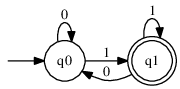
\includegraphics[width=0.3\linewidth,height=\textheight,keepaspectratio]{chapters/images/afd1.png}

}

\caption{\label{fig-afd1}Autômato de Estados Finitos Determinístico.}

\end{figure}%

O autômato da Figura~\ref{fig-afd1} possui dois estados, \(q_0\) e
\(q_1\), sendo \(q_0\) o estado inicial e \(q_1\) um estado final. As
setas indicam como o autômato deve mudar de estado à medida que os
símbolos da palavra são lidos.

Por exemplo, quando o autômato está no estado \(q_0\) e lê o símbolo
\(0\), permanece em \(q_0\). Quando está em \(q_0\) e lê o símbolo
\(1\), realiza uma transição para \(q_1\). A partir de \(q_1\), as
transições dependem dos símbolos definidos no autômato.

Essa representação permite visualizar o comportamento da máquina, mas,
para descrever formalmente uma computação, é necessário definir o que
significa o autômato estar em determinado estado enquanto ainda existem
símbolos a serem processados.

\subsection{Configuração
instantânea}\label{configurauxe7uxe3o-instantuxe2nea}

Para representar uma computação, podemos utilizar o conceito de
\textbf{configuração instantânea}. Uma configuração instantânea descreve
a situação do autômato em um determinado instante da computação e é
representada pelo par

\[
[e,w],
\]

em que:

\begin{itemize}
\tightlist
\item
  \(e\) representa o \textbf{estado atual} do autômato;
\item
  \(w\) representa a parte da palavra que ainda não foi processada.
\end{itemize}

Por exemplo,

\[
[q_0,001]
\]

indica que o autômato está no estado \(q_0\) e que ainda precisa
processar a palavra \(001\).

À medida que os símbolos são lidos, a configuração é modificada. Para
representar essa transformação, utiliza-se a relação

\[
\vdash,
\]

denominada \textbf{relação de transição} ou \textbf{relação de
computação}.

Suponha que exista no autômato uma transição de \(q_0\) para \(q_1\)
associada ao símbolo \(a\). Nesse caso, podemos representar a computação
por

\[
[q_0,aw]\vdash[q_1,w].
\]

A expressão indica que o autômato estava no estado \(q_0\), tinha como
próximo símbolo a ser lido o símbolo \(a\) e, após processá-lo, passou
para o estado \(q_1\). A parte \(w\) permanece como a porção da palavra
que ainda não foi processada.

Portanto, cada passo da computação consome exatamente um símbolo da
palavra e produz uma nova configuração.

\subsubsection{Computação de uma
palavra}\label{computauxe7uxe3o-de-uma-palavra}

Considere novamente o autômato apresentado na Figura~\ref{fig-afd1} e a
palavra

\[
w=001.
\]

A computação pode ser representada por uma sequência de configurações
instantâneas:

\[
[q_0,001]
\vdash
[q_0,01]
\vdash
[q_0,1]
\vdash
[q_1,\varepsilon].
\]

No primeiro passo, o autômato está em \(q_0\) e lê o primeiro símbolo,
que é \(0\). De acordo com a transição correspondente, permanece em
\(q_0\). A palavra restante passa a ser \(01\).

No segundo passo, o autômato lê novamente o símbolo \(0\) e permanece em
\(q_0\). A palavra restante passa a ser \(1\).

Finalmente, o autômato lê o símbolo \(1\) e realiza a transição para o
estado \(q_1\). Nesse momento, todos os símbolos da palavra foram
processados.

Os símbolos \(\lambda\) ou \(\varepsilon\) são utilizados para
representar a \textbf{palavra vazia}. Neste livro, será utilizada
preferencialmente a notação \(\varepsilon\), embora \(\lambda\) também
seja encontrada na literatura.

Assim,

\[
\lambda=\varepsilon
\]

e

\[
|\varepsilon|=0.
\]

Quando a computação termina, a configuração

\[
[q_1,\varepsilon]
\]

indica que o autômato está no estado \(q_1\) e não existem mais símbolos
para serem processados.

\subsubsection{Aceitação de uma
palavra}\label{aceitauxe7uxe3o-de-uma-palavra}

Uma palavra é \textbf{aceita} por um autômato finito quando a computação
começa no estado inicial, todos os símbolos da palavra são processados e
o autômato termina em um estado final.

No exemplo anterior, como \(q_0\) é o estado inicial e \(q_1\) é um
estado final, a palavra \(001\) é aceita pelo autômato.

Por outro lado, se após o processamento do último símbolo o autômato
terminar em um estado que não seja final, a palavra será rejeitada.

É importante observar que o fato de o autômato passar por um estado
final durante a computação não é suficiente para aceitar uma palavra. O
autômato deve \textbf{terminar a leitura de toda a palavra em um estado
final}.

\subsubsection{Computação completa}\label{computauxe7uxe3o-completa}

Para representar vários passos de uma computação, utilizamos a relação
\(\vdash^*\), denominada \textbf{fecho reflexivo e transitivo} da
relação \(\vdash\).

Assim,

\[
[e,w]\vdash^*[e',w']
\]

significa que é possível transformar a configuração \([e,w]\) na
configuração \([e',w']\) após \textbf{zero ou mais passos} de
computação.

O uso do asterisco é importante porque permite representar também uma
computação que não realiza nenhum passo. Dessa forma,

\[
[e,w]\vdash^*[e,w].
\]

No caso de uma palavra ser processada completamente, temos uma
computação da forma

\[
[i,w]\vdash^*[f,\epsilon],
\]

em que \(i\) é o estado inicial e \(f\) é um estado final.

\subsubsection{Linguagem reconhecida por um
autômato}\label{linguagem-reconhecida-por-um-autuxf4mato}

Um autômato finito não reconhece apenas uma palavra. Ao ser utilizado
sobre todas as palavras possíveis do alfabeto \(\Sigma\), ele determina
um conjunto de palavras que são aceitas. Esse conjunto é denominado
\textbf{linguagem reconhecida} ou \textbf{linguagem aceita} pelo
autômato.

Seja \(A\) um autômato finito definido sobre o alfabeto \(\Sigma\). A
linguagem reconhecida por \(A\) é denotada por \(L(A)\) e pode ser
definida formalmente por

\[
L(A)=
\{w\in\Sigma^*
\mid
[i,w]\vdash^*[f,\epsilon],
\text{ para algum } f\in F
\}.
\]

Nessa definição:

\begin{itemize}
\tightlist
\item
  \(L(A)\) é a linguagem reconhecida pelo autômato \(A\);
\item
  \(w\) é uma palavra pertencente ao alfabeto \(\Sigma^*\);
\item
  \(i\) é o estado inicial do autômato;
\item
  \(F\) é o conjunto de estados finais;
\item
  \(f\) é um estado final, isto é, \(f\in F\);
\item
  \(\epsilon\) representa a palavra vazia;
\item
  \(\vdash^*\) representa zero ou mais passos da computação.
\end{itemize}

A expressão

\[
[i,w]\vdash^*[f,\epsilon]
\]

significa, portanto, que o autômato começa no estado inicial \(i\),
processa completamente a palavra \(w\) e termina em algum estado final
\(f\).

\subsection{Autômatos Finitos
Determinísticos}\label{autuxf4matos-finitos-determinuxedsticos}

Os \textbf{Autômatos Finitos Determinísticos (AFDs)} constituem um dos
modelos mais simples de máquinas abstratas utilizadas para reconhecer
linguagens formais. Um AFD processa uma palavra símbolo por símbolo,
mantendo, a cada instante, um único estado corrente. Para cada
combinação de estado e símbolo de entrada existe \textbf{exatamente uma
transição possível}.

A palavra \emph{determinístico} está relacionada justamente a essa
característica. Dado o estado atual do autômato e o próximo símbolo da
palavra, o próximo estado é determinado de maneira única. Portanto, não
existe escolha entre diferentes caminhos possíveis durante a computação.

Essa propriedade torna os AFDs particularmente adequados para
implementação em programas de computador. O processamento de uma palavra
pode ser realizado simplesmente consultando uma tabela que associa cada
par formado por um estado e um símbolo de entrada ao próximo estado.

\subsubsection{Definição formal}\label{definiuxe7uxe3o-formal}

O Autômato Finito Determinístico (AFD) é matematicamente definido como
uma quíntupla.

\begin{definition}[]\protect\hypertarget{def-afd}{}\label{def-afd}

Um \textbf{Autômato Finito Determinístico (AFD)} é uma quíntupla

\[
A=(Q,\Sigma,\delta,i,F),
\]

onde:

\begin{itemize}
\tightlist
\item
  \(Q\) é um conjunto finito de \textbf{estados} do autômato;
\item
  \(\Sigma\) é o \textbf{alfabeto de entrada};
\item
  \(\delta:Q\times\Sigma\rightarrow Q\) é a \textbf{função de
  transição};
\item
  \(i\in Q\) é o \textbf{estado inicial};
\item
  \(F\subseteq Q\) é o conjunto de \textbf{estados finais}.
\end{itemize}

\end{definition}

Cada componente da quíntupla possui uma função específica na definição
do comportamento do autômato.

O conjunto \(E\) contém todos os estados possíveis da máquina. Como se
trata de um autômato finito, esse conjunto deve possuir uma quantidade
finita de elementos. Por exemplo,

\[
Q=\{q_0,q_1,q_2\}.
\]

O conjunto \(\Sigma\) corresponde ao alfabeto utilizado como entrada. Se
o autômato reconhece palavras constituídas pelos símbolos \(0\) e \(1\),
podemos ter

\[
\Sigma=\{0,1\}.
\]

A função \(\delta\) determina como o autômato muda de estado. Como

\[
\delta:Q\times\Sigma\rightarrow Q,
\]

para cada estado \(q\in E\) e cada símbolo \(a\in\Sigma\), existe
exatamente um estado \(p\in E\) tal que

\[
\delta(q,a)=p.
\]

Essa é justamente a característica que diferencia o AFD de modelos não
determinísticos: \textbf{cada par (estado, símbolo) possui uma única
transição definida}.

O estado \(i\) representa o estado em que a computação começa.
Finalmente, o conjunto \(F\) contém os estados que representam uma
computação de aceitação. Uma palavra será aceita quando, depois de todos
os seus símbolos serem processados, o autômato estiver em algum estado
pertencente a \(F\).

\subsubsection{Exemplo de um AFD}\label{exemplo-de-um-afd}

Usando a definição anterior, podemos descrever formalmente a máquina
apresentada na Figura~\ref{fig-afd1} como

\[
A_1=
(\{q_0,q_1\},
\{0,1\},
\delta,
q_0,
\{q_1\}).
\]

Nesse caso,

\[
Q=\{q_0,q_1\},
\]

é o conjunto de estados;

\[
\Sigma=\{0,1\},
\]

é o alfabeto de entrada;

\[
i=q_0
\]

é o estado inicial; e

\[
F=\{q_1\}
\]

é o conjunto de estados finais.

A função de transição \(\delta\) pode ser representada por uma tabela.
Nas linhas são apresentados os estados e nas colunas os símbolos do
alfabeto.

\begin{longtable}[]{|c|c|c|}

\caption{\label{tbl-transicao}Função de transição \(\delta\)}

\tabularnewline

\toprule\noalign{}
\(\delta\) & \(0\) & \(1\) \\
\midrule\noalign{}
\endhead
\bottomrule\noalign{}
\endlastfoot
\(q_0\) & \(q_0\) & \(q_1\) \\
\midrule
\(q_1\) & \(q_0\) & \(q_1\) \\

\end{longtable}

A tabela deve ser interpretada da seguinte maneira. Para determinar o
próximo estado, basta localizar a linha correspondente ao estado atual e
a coluna correspondente ao símbolo que está sendo lido.

Por exemplo,

\[
\delta(q_0,0)=q_0
\]

indica que, estando no estado \(q_0\) e lendo o símbolo \(0\), o
autômato permanece em \(q_0\).

Da mesma forma,

\[
\delta(q_0,1)=q_1
\]

indica que, estando em \(q_0\) e lendo o símbolo \(1\), o autômato passa
para \(q_1\).

Podemos ainda observar que

\[
\delta(q_1,0)=q_0
\]

e

\[
\delta(q_1,1)=q_1.
\]

A tabela contém uma entrada para cada combinação entre estado e símbolo
do alfabeto. Essa propriedade é uma consequência direta da definição de
um AFD: a função

\[
\delta:Q\times\Sigma\rightarrow Q
\]

é uma função \textbf{total}. Portanto, não pode existir um par \((q,a)\)
para o qual \(\delta(q,a)\) não esteja definido.

\subsubsection{Função de transição
estendida}\label{funuxe7uxe3o-de-transiuxe7uxe3o-estendida}

A função \(\delta\) permite determinar apenas o próximo estado do
autômato após a leitura de \textbf{um único símbolo}. Entretanto,
durante a computação de uma palavra, precisamos determinar o estado
alcançado após a leitura de toda a palavra.

Para isso, definimos a \textbf{função de transição estendida},
normalmente representada por \(\hat{\delta}\).

\begin{definition}[]\protect\hypertarget{def-transicao-estendida}{}\label{def-transicao-estendida}

Seja um AFD \(A = (Q,\Sigma,\delta,i,F)\). A função de transição
estendida para \(A\),
\(\hat{\delta} : Q \times \Sigma^* \rightarrow Q\), definida
recursivamente como:

\begin{itemize}
\item
  \(\hat{\delta}(q,\varepsilon) = q\)
\item
  \(\hat{\delta}(q,ay) = \hat{\delta}(\delta(q,a),y)\), para todo
  \(q \in Q\), \(a \in \Sigma\) e \(y \in \Sigma^*\)
\end{itemize}

\end{definition}

A primeira regra estabelece o caso base da definição. Se a palavra a ser
processada é vazia, o autômato permanece no estado em que se encontra:

\[
\hat{\delta}(q,\varepsilon)=q.
\]

A segunda regra determina como processar uma palavra não vazia. Se a
palavra é formada por um primeiro símbolo \(a\) seguido da palavra
\(y\), primeiro aplicamos \(\delta\) para processar \(a\) e obter o novo
estado. Em seguida, aplicamos recursivamente \(\hat{\delta}\) para
processar os símbolos restantes.

Em outras palavras, enquanto \(\delta\) processa \textbf{um símbolo},
\(\hat{\delta}\) permite processar \textbf{uma palavra inteira}.

Essa distinção pode ser resumida por:

\[
\delta:Q\times\Sigma\rightarrow Q
\]

e

\[
\hat{\delta}:Q\times\Sigma^*\rightarrow Q.
\]

Observe que o domínio da primeira função utiliza \(\Sigma\), enquanto o
domínio da segunda utiliza \(\Sigma^*\).

\subsubsection{\texorpdfstring{Exemplo de computação utilizando
\(\hat{\delta}\)}{Exemplo de computação utilizando \textbackslash hat\{\textbackslash delta\}}}\label{exemplo-de-computauxe7uxe3o-utilizando-hatdelta}

Considere novamente o autômato \(A_1\) e a palavra

\[
w=001.
\]

A aplicação da função de transição estendida pode ser desenvolvida passo
a passo:

\[
\begin{aligned}
\hat{\delta}(q_0,001)
&=\hat{\delta}(\delta(q_0,0),01)\\
&=\hat{\delta}(q_0,01)\\
&=\hat{\delta}(\delta(q_0,0),1)\\
&=\hat{\delta}(q_0,1)\\
&=\hat{\delta}(\delta(q_0,1),\epsilon)\\
&=\hat{\delta}(q_1,\epsilon)\\
&=q_1.
\end{aligned}
\]

Portanto,

\[
\boxed{\hat{\delta}(q_0,001)=q_1}.
\]

Como \(q_1\in F\), concluímos que a palavra \(001\) é aceita pelo
autômato \(A_1\).

Esse resultado também pode ser expresso utilizando a relação entre
configurações instantâneas:

\[
[q_0,001]
\vdash
[q_0,01]
\vdash
[q_0,1]
\vdash
[q_1,\epsilon].
\]

As duas formas de representação descrevem a mesma computação. A primeira
utiliza a função de transição estendida e a segunda explicita cada
configuração intermediária do autômato.

\subsubsection{Critério de
aceitação}\label{crituxe9rio-de-aceitauxe7uxe3o}

A função de transição estendida permite definir a linguagem reconhecida
por um AFD de maneira particularmente simples.

Seja

\[
A=(Q,\Sigma,\delta,i,F).
\]

A palavra \(w\in\Sigma^*\) é aceita por \(A\) se, e somente se,

\[
\hat{\delta}(i,w)\in F.
\]

Consequentemente, a linguagem reconhecida por \(A\) é dada por

\[
L(A)=
\{w\in\Sigma^*
\mid
\hat{\delta}(i,w)\in F
\}.
\]

Essa definição é equivalente à definição baseada nas configurações
instantâneas apresentada anteriormente. A diferença está apenas na forma
de representar a computação.

Para o autômato \(A_1\), por exemplo,

\[
\hat{\delta}(q_0,001)=q_1
\]

e

\[
q_1\in F.
\]

Logo,

\[
001\in L(A_1).
\]

Por outro lado, para a palavra \(000\) temos

\[
\hat{\delta}(q_0,000)=q_0.
\]

Como

\[
q_0\notin F,
\]

temos

\[
000\notin L(A_1).
\]

\subsubsection{Implementação da
computação}\label{implementauxe7uxe3o-da-computauxe7uxe3o}

A definição matemática de um AFD possui uma correspondência direta com
sua implementação computacional. Para simular o autômato, basta manter
uma variável contendo o \textbf{estado atual} e, para cada símbolo da
palavra de entrada, consultar a função de transição.

A tabela apresentada na Tabela~\ref{tbl-transicao} pode ser implementada
diretamente como uma matriz. As linhas representam os estados e as
colunas representam os símbolos do alfabeto.

Uma versão simplificada do algoritmo pode ser descrita pelo seguinte
código exemplo:

\begin{Shaded}
\begin{Highlighting}[]
\PreprocessorTok{\#include }\ImportTok{\textless{}stdio.h\textgreater{}}
\CommentTok{// definição do automato}
\CommentTok{// M = (Q, Sigma, T, q\_0, F)}
\DataTypeTok{char} \OperatorTok{*}\NormalTok{estados }\OperatorTok{=} \StringTok{"01"}\OperatorTok{;}
\DataTypeTok{char} \OperatorTok{*}\NormalTok{alfabeto }\OperatorTok{=} \StringTok{"01"}\OperatorTok{;}
\DataTypeTok{int}\NormalTok{ T}\OperatorTok{[}\DecValTok{2}\OperatorTok{][}\DecValTok{2}\OperatorTok{]} \OperatorTok{=} \OperatorTok{\{}\DecValTok{0}\OperatorTok{,} \DecValTok{1}\OperatorTok{,}
               \DecValTok{0}\OperatorTok{,} \DecValTok{1}\OperatorTok{\};}
\DataTypeTok{char}\NormalTok{ inicial }\OperatorTok{=} \DecValTok{0}\OperatorTok{;}
\DataTypeTok{char} \OperatorTok{*}\NormalTok{finais }\OperatorTok{=} \StringTok{"1"}\OperatorTok{;}

\DataTypeTok{int}\NormalTok{ pertence}\OperatorTok{(}\DataTypeTok{int}\NormalTok{ s}\OperatorTok{,} \DataTypeTok{char} \OperatorTok{*}\NormalTok{c}\OperatorTok{)}
\OperatorTok{\{}
    \DataTypeTok{int}\NormalTok{ i}\OperatorTok{;}
    \ControlFlowTok{for} \OperatorTok{(}\NormalTok{i }\OperatorTok{=} \DecValTok{0}\OperatorTok{;}\NormalTok{ c}\OperatorTok{[}\NormalTok{i}\OperatorTok{];}\NormalTok{ i}\OperatorTok{++)}
        \ControlFlowTok{if} \OperatorTok{(}\NormalTok{s }\OperatorTok{==}\NormalTok{ c}\OperatorTok{[}\NormalTok{i}\OperatorTok{]} \OperatorTok{{-}} \CharTok{\textquotesingle{}0\textquotesingle{}}\OperatorTok{)}
            \ControlFlowTok{return} \DecValTok{1}\OperatorTok{;}
    \ControlFlowTok{return} \DecValTok{0}\OperatorTok{;}
\OperatorTok{\}}

\DataTypeTok{int}\NormalTok{ main}\OperatorTok{()}
\OperatorTok{\{}
    \DataTypeTok{char}\NormalTok{ entrada}\OperatorTok{[}\DecValTok{20}\OperatorTok{];}
    \ControlFlowTok{do}
    \OperatorTok{\{}
\NormalTok{        printf}\OperatorTok{(}\StringTok{"Cadeia de entrada (usando o alfabeto: }\SpecialCharTok{\%s}\StringTok{): "}\OperatorTok{,}\NormalTok{ alfabeto}\OperatorTok{);}
\NormalTok{        scanf}\OperatorTok{(}\StringTok{"}\SpecialCharTok{\%s}\StringTok{"}\OperatorTok{,}\NormalTok{ entrada}\OperatorTok{);}
\NormalTok{        printf}\OperatorTok{(}\StringTok{"|}\SpecialCharTok{\%s}\StringTok{|}\SpecialCharTok{\textbackslash{}n}\StringTok{"}\OperatorTok{,}\NormalTok{ entrada}\OperatorTok{);}
        \ControlFlowTok{if} \OperatorTok{(}\NormalTok{entrada}\OperatorTok{[}\DecValTok{0}\OperatorTok{]} \OperatorTok{!=} \CharTok{\textquotesingle{}.\textquotesingle{}}\OperatorTok{)}
        \OperatorTok{\{}
            \DataTypeTok{int}\NormalTok{ i }\OperatorTok{=} \DecValTok{0}\OperatorTok{;}
            \DataTypeTok{int}\NormalTok{ estado }\OperatorTok{=}\NormalTok{ inicial}\OperatorTok{;}
            \ControlFlowTok{while} \OperatorTok{(}\NormalTok{entrada}\OperatorTok{[}\NormalTok{i}\OperatorTok{])}
            \OperatorTok{\{}
\NormalTok{                estado }\OperatorTok{=}\NormalTok{ T}\OperatorTok{[}\NormalTok{estado}\OperatorTok{][}\NormalTok{entrada}\OperatorTok{[}\NormalTok{i}\OperatorTok{]} \OperatorTok{{-}} \CharTok{\textquotesingle{}a\textquotesingle{}}\OperatorTok{];}
\NormalTok{                i}\OperatorTok{++;}
            \OperatorTok{\}}
            \ControlFlowTok{if} \OperatorTok{(}\NormalTok{pertence}\OperatorTok{(}\NormalTok{estado}\OperatorTok{,}\NormalTok{ finais}\OperatorTok{))}
\NormalTok{                puts}\OperatorTok{(}\StringTok{"aceita!"}\OperatorTok{);}
            \ControlFlowTok{else}
\NormalTok{                puts}\OperatorTok{(}\StringTok{"rejeita"}\OperatorTok{);}
        \OperatorTok{\}}
    \OperatorTok{\}} \ControlFlowTok{while} \OperatorTok{(}\NormalTok{entrada}\OperatorTok{[}\DecValTok{0}\OperatorTok{]} \OperatorTok{!=} \CharTok{\textquotesingle{}.\textquotesingle{}}\OperatorTok{);}
    \ControlFlowTok{return} \DecValTok{0}\OperatorTok{;}
\OperatorTok{\}}
\end{Highlighting}
\end{Shaded}

Para a palavra \(w=001\), o algoritmo executa três iterações:

\begin{longtable*}[]{|c|c|c|c|}
\toprule\noalign{}
Passo & Estado atual & Símbolo & Próximo estado \\
\midrule\noalign{}
\endhead
\bottomrule\noalign{}
\endlastfoot
1 & \(q_0\) & \(0\) & \(q_0\) \\
\midrule
2 & \(q_0\) & \(0\) & \(q_0\) \\
\midrule
3 & \(q_0\) & \(1\) & \(q_1\) \\
\end{longtable*}

Ao final do processamento, o estado atual é \(q_1\). Como \(q_1\)
pertence ao conjunto de estados finais,

\[
q_1\in F,
\]

a palavra é aceita.

Essa implementação evidencia uma das principais vantagens dos AFDs:
\textbf{o reconhecimento de uma palavra pode ser realizado de maneira
extremamente simples, processando cada símbolo uma única vez}.

Se a palavra possui comprimento \(n\), o algoritmo realiza exatamente
\(n\) consultas à função de transição. Assim, considerando que a
consulta à tabela de transição seja realizada em tempo constante, o
reconhecimento de uma palavra possui complexidade temporal

\[
O(n),
\]

em que \(n=|w|\).

Essa característica explica, em parte, a importância dos autômatos
finitos na implementação de analisadores léxicos. Uma vez construído o
AFD correspondente a um determinado padrão léxico, a sequência de
caracteres pode ser processada de forma eficiente, realizando uma
transição para cada símbolo lido.

Nos exemplos computacionais apresentados neste livro, a função
\(\delta\) será frequentemente representada por uma tabela ou por uma
estrutura de dados equivalente. Dessa forma, a definição matemática do
AFD pode ser diretamente transformada em um algoritmo de simulação.

\subsubsection{Fechamento sob a operação de
união}\label{sec-fechamento-uniao}

Uma propriedade importante das linguagens regulares é o
\textbf{fechamento sob operações}. Dizer que uma classe de linguagens é
fechada sob determinada operação significa que, ao aplicarmos essa
operação a linguagens pertencentes à classe, o resultado também pertence
à mesma classe.

No caso da união, queremos demonstrar que a união de duas linguagens
regulares é sempre uma linguagem regular.

\begin{theorem}[]\protect\hypertarget{thm-fechamento-uniao}{}\label{thm-fechamento-uniao}

A classe das linguagens regulares é \textbf{fechada sob a operação de
união}.

\end{theorem}

Em outras palavras, se \(A_1\) e \(A_2\) são linguagens regulares sobre
um mesmo alfabeto \(\Sigma\), então a linguagem

\[
A = A_1 \cup A_2
\]

também é regular.

\paragraph{Ideia da demonstração}\label{ideia-da-demonstrauxe7uxe3o}

Como \(A_1\) e \(A_2\) são regulares, existem autômatos finitos
determinísticos que reconhecem essas linguagens. A ideia é construir um
novo autômato que simule os dois autômatos simultaneamente, processando
a mesma palavra.

A cada símbolo lido, o novo autômato atualiza o estado correspondente de
cada um dos autômatos originais. Assim, ele mantém a informação sobre o
estado em que cada máquina estaria após processar o prefixo da palavra
que já foi lido.

Para reconhecer a união, basta definir que o novo autômato aceita uma
palavra quando \textbf{pelo menos um dos autômatos originais aceita essa
palavra}.

\paragraph{Prova por construção}\label{prova-por-construuxe7uxe3o-1}

Sejam

\[
M_1 = (Q_1, \Sigma, \delta_1, q_1, F_1)
\]

e

\[
M_2 = (Q_2, \Sigma, \delta_2, q_2, F_2)
\]

dois autômatos finitos determinísticos que reconhecem, respectivamente,
as linguagens \(A_1\) e \(A_2\).

Construiremos um autômato determinístico

\[
M = (Q, \Sigma, \delta, q_0, F)
\]

tal que \(L(M) = A_1 \cup A_2\).

A construção é definida da seguinte forma.

\paragraph{Conjunto de estados}\label{conjunto-de-estados}

O conjunto de estados de \(M\) é o produto cartesiano dos conjuntos de
estados dos autômatos originais:

\[
Q = Q_1 \times Q_2.
\]

Portanto, cada estado de \(M\) é um par \((r_1, r_2)\), em que
\(r_1 \in Q_1\) e \(r_2 \in Q_2\).

A primeira componente representa o estado atual de \(M_1\), enquanto a
segunda representa o estado atual de \(M_2\). Dessa maneira, cada estado
do novo autômato registra simultaneamente as configurações dos dois
autômatos durante o processamento da palavra.

Se \(M_1\) possui \(m\) estados e \(M_2\) possui \(n\) estados, então
\(M\) possui \(mn\) estados, embora nem todos precisem ser alcançáveis a
partir do estado inicial.

\paragraph{Alfabeto de entrada}\label{alfabeto-de-entrada}

O alfabeto de entrada de \(M\) é o mesmo dos autômatos originais, isto
é, \(\Sigma\).

Essa hipótese simplifica a construção. Caso os autômatos tenham
alfabetos diferentes, podemos considerar o alfabeto comum
\(\Sigma = \Sigma_1 \cup \Sigma_2\) e completar as funções de transição
para os símbolos ausentes, utilizando estados não finais de erro, quando
necessário.

\paragraph{Função de transição}\label{funuxe7uxe3o-de-transiuxe7uxe3o}

A função de transição de \(M\) é definida por

\[
\delta((r_1,r_2),a)
=
\bigl(\delta_1(r_1,a),\delta_2(r_2,a)\bigr),
\]

para todo \((r_1,r_2) \in Q\) e todo \(a \in \Sigma\).

Isso significa que, ao ler um símbolo \(a\), o novo autômato executa
simultaneamente as transições que seriam realizadas por \(M_1\) e
\(M_2\). A primeira componente do par é atualizada de acordo com
\(\delta_1\), e a segunda, de acordo com \(\delta_2\).

\paragraph{Estado inicial}\label{estado-inicial}

O estado inicial de \(M\) é o par formado pelos estados iniciais dos
autômatos originais:

\[
q_0 = (q_1,q_2).
\]

Assim, antes da leitura de qualquer símbolo, cada componente do novo
estado corresponde ao estado inicial de seu respectivo autômato.

\paragraph{Conjunto de estados finais}\label{conjunto-de-estados-finais}

Para reconhecer a união, definimos o conjunto de estados finais como

\[
F =
\{(r_1,r_2) \in Q
\mid r_1 \in F_1 \text{ ou } r_2 \in F_2\}.
\]

A palavra \emph{ou} nessa definição representa a disjunção lógica
inclusiva: basta que pelo menos uma das componentes do par seja um
estado final do respectivo autômato original.

Equivalentemente, podemos escrever

\[
F = (F_1 \times Q_2) \cup (Q_1 \times F_2).
\]

Portanto, um estado do autômato produto é final quando a primeira
componente pertence a \(F_1\), quando a segunda componente pertence a
\(F_2\), ou quando ambas pertencem aos respectivos conjuntos de estados
finais.

\paragraph{Verificação da
construção}\label{verificauxe7uxe3o-da-construuxe7uxe3o}

Considere uma palavra \(w \in \Sigma^*\). Como a função de transição de
\(M\) atualiza simultaneamente as duas componentes, após a leitura de
\(w\), o estado alcançado é

\[
\hat{\delta}(q_0,w)
=
\bigl(\hat{\delta_1}(q_1,w),\hat{\delta_2}(q_2,w)\bigr),
\]

em que \(\hat{\delta}\), \(\hat{\delta_1}\) e \(\hat{\delta_2}\) são as
extensões das respectivas funções de transição para palavras.

Pela definição de \(F\), o autômato \(M\) aceita \(w\) se, e somente se,
pelo menos uma das componentes do par ordenado do estado alcançado é
final. Logo,

\[
\begin{aligned}
w \in L(M)
&\iff w \in A_1 \text{ ou } w \in A_2\\
&\iff w \in A_1 \cup A_2.
\end{aligned}
\]

Concluímos que

\[
L(M) = A_1 \cup A_2.
\]

Como construímos um autômato finito determinístico que reconhece
\(A_1 \cup A_2\), essa linguagem é regular. Portanto, a classe das
linguagens regulares é fechada sob a operação de união.

\[
\boxed{L(M) = A_1 \cup A_2}
\]

\paragraph{Observação: união e
interseção}\label{observauxe7uxe3o-uniuxe3o-e-interseuxe7uxe3o}

É importante distinguir a condição de aceitação usada na união daquela
utilizada na interseção.

\textbf{União:} o estado produto é final se pelo menos uma das
componentes é final:

\[
F_{\cup} = (F_1 \times Q_2) \cup (Q_1 \times F_2).
\]

\textbf{Interseção:} o estado produto é final somente se ambas as
componentes são finais:

\[
F_{\cap} = F_1 \times F_2.
\]

Portanto, a mesma construção de estados e de transições pode ser
utilizada para reconhecer a união ou a interseção de duas linguagens
regulares. A diferença está apenas na definição do conjunto de estados
finais.

\subsubsection{Exemplo: construção de um AFD para a união de duas
linguagens regulares}\label{sec-exemplo-uniao-afd}

Para compreender a construção apresentada na prova do fechamento sob a
união, considere duas linguagens regulares sobre o alfabeto
\(\Sigma=\{a,b\}\):

\begin{itemize}
\tightlist
\item
  \(A_1\): conjunto das palavras que terminam com o símbolo \(a\);
\item
  \(A_2\): conjunto das palavras que terminam com o símbolo \(b\).
\end{itemize}

Nosso objetivo é construir um autômato finito determinístico que
reconheça a linguagem \(A=A_1\cup A_2\).

\paragraph{\texorpdfstring{Primeiro autômato: palavras que terminam em
\texttt{a}}{Primeiro autômato: palavras que terminam em a}}\label{primeiro-autuxf4mato-palavras-que-terminam-em-a}

O primeiro autômato, denominado \(M_1\), reconhece as palavras que
terminam com o símbolo \(a\). Para isso, utiliza dois estados:

\begin{itemize}
\tightlist
\item
  \(q_0\): estado inicial e não final, que representa uma palavra vazia
  ou um prefixo cuja última letra é \(b\);
\item
  \(q_1\): estado final, que representa uma palavra cuja última letra é
  \(a\).
\end{itemize}

A função de transição é definida de modo que a leitura de \(a\) conduza
ao estado \(q_1\), enquanto a leitura de \(b\) conduza ao estado
\(q_0\). Consequentemente, após a leitura completa de uma palavra, o
autômato estará em \(q_1\) se, e somente se, a palavra terminar em
\(a\).

A Figura~\ref{fig-afd1-a} contém a representação desse autômato.

\begin{figure}

\centering{

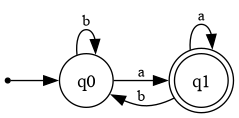
\includegraphics[width=0.3\linewidth,height=\textheight,keepaspectratio]{chapters/images/afd1-a.png}

}

\caption{\label{fig-afd1-a}Autômato \(A_1\)}

\end{figure}%

\paragraph{\texorpdfstring{Segundo autômato: palavras que terminam em
\texttt{b}}{Segundo autômato: palavras que terminam em b}}\label{segundo-autuxf4mato-palavras-que-terminam-em-b}

O segundo autômato, denominado \(M_2\), reconhece as palavras que
terminam com o símbolo \(b\). Sua estrutura é semelhante à do primeiro
autômato:

\begin{itemize}
\tightlist
\item
  \(p_0\): estado inicial e não final, que representa uma palavra vazia
  ou um prefixo cuja última letra é \(a\);
\item
  \(p_1\): estado final, que representa uma palavra cuja última letra é
  \(b\).
\end{itemize}

Ao ler \(a\), o autômato passa para \(p_0\); ao ler \(b\), passa para
\(p_1\). Portanto, uma palavra é aceita por \(M_2\) se, e somente se,
terminar em \(b\).

A Figura~\ref{fig-afd2-b} apresenta a representação gráfica desse
autômato.

\begin{figure}

\centering{

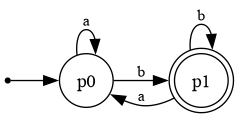
\includegraphics[width=0.3\linewidth,height=\textheight,keepaspectratio]{chapters/images/afd2-b.png}

}

\caption{\label{fig-afd2-b}Autômato \(A_2\)}

\end{figure}%

\paragraph{Construção do autômato
produto}\label{construuxe7uxe3o-do-autuxf4mato-produto}

Para reconhecer a união das duas linguagens, construímos um terceiro
autômato \(M\) que simula \(M_1\) e \(M_2\) simultaneamente.

O conjunto de estados é o produto cartesiano:

\[
Q=Q_1\times Q_2.
\]

Como \(Q_1=\{q_0,q_1\}\) e \(Q_2=\{p_0,p_1\}\), obtemos:

\[
Q=\{
(q_0,p_0),
(q_0,p_1),
(q_1,p_0),
(q_1,p_1)
\}.
\]

Cada estado representa a situação dos dois autômatos originais após a
leitura do mesmo prefixo da palavra.

Por exemplo, o estado \((q_1,p_0)\) indica que \(M_1\) está em seu
estado final, enquanto \(M_2\) está em seu estado não final. Isso
significa que a palavra processada termina em \(a\), sendo aceita por
\(M_1\).

Já o estado \((q_0,p_1)\) indica que a palavra termina em \(b\), sendo
aceita por \(M_2\).

O estado inicial do autômato produto é:

\[
q_0'=(q_0,p_0).
\]

A função de transição é calculada componente a componente. Assim,

\[
\delta((r_1,r_2),x)
=
(\delta_1(r_1,x),\delta_2(r_2,x)).
\]

Considere, por exemplo, a leitura do símbolo \(a\) a partir do estado
inicial. No primeiro autômato, a transição é de \(q_0\) para \(q_1\); no
segundo, é de \(p_0\) para \(p_0\). Logo,

\[
\delta((q_0,p_0),a)=(q_1,p_0).
\]

De modo semelhante, ao ler \(b\), temos:

\[
\delta((q_0,p_0),b)=(q_0,p_1).
\]

A tabela a seguir apresenta todas as transições do autômato produto.

\begin{longtable*}[]{|l|l|l|}
\toprule\noalign{}
Estado & Entrada \texttt{a} & Entrada \texttt{b} \\
\midrule\noalign{}
\endhead
\bottomrule\noalign{}
\endlastfoot
\((q_0,p_0)\) & \((q_1,p_0)\) & \((q_0,p_1)\) \\
\midrule
\((q_1,p_0)\) & \((q_1,p_0)\) & \((q_0,p_1)\) \\
\midrule
\((q_0,p_1)\) & \((q_1,p_0)\) & \((q_0,p_1)\) \\
\midrule
\((q_1,p_1)\) & \((q_1,p_0)\) & \((q_0,p_1)\) \\
\end{longtable*}

\paragraph{Definição dos estados
finais}\label{definiuxe7uxe3o-dos-estados-finais}

Como queremos reconhecer a união \(A_1\cup A_2\), um estado do autômato
produto será final quando pelo menos uma de suas componentes for final.

Portanto,

\[
F=(F_1\times Q_2)\cup(Q_1\times F_2).
\]

Nesse exemplo, \(F_1=\{q_1\}\) e \(F_2=\{p_1\}\). Assim, o conjunto de
estados finais é:

\[
F=\{
(q_1,p_0),
(q_0,p_1),
(q_1,p_1)
\}.
\]

O estado \((q_1,p_1)\) pertence à definição formal do conjunto de
estados finais, pois ambas as componentes são finais. Entretanto, esse
estado é inalcançável: uma palavra sobre \(\{a,b\}\) não pode terminar
simultaneamente em \(a\) e em \(b\).

A Figura~\ref{fig-uniao} contém a representação gráfica do autômato
produto, incluindo os quatro estados definidos pela construção
cartesiana.

\begin{figure}

{\centering 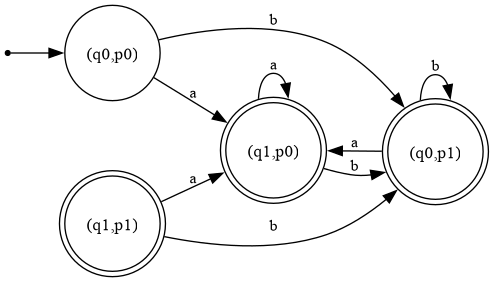
\includegraphics[width=0.5\linewidth,height=\textheight,keepaspectratio]{chapters/images/afd-uniao.png}

}

\caption{Autômato união de \(A_1\) e \(A_2\)}

\end{figure}%

\paragraph{Simulação do
reconhecimento}\label{simulauxe7uxe3o-do-reconhecimento}

Para verificar o funcionamento do autômato produto, considere algumas
palavras de entrada.

\begin{longtable*}[]{|l|l|l|}
\toprule\noalign{}
Palavra & Estado final alcançado & Resultado \\
\midrule\noalign{}
\endhead
\bottomrule\noalign{}
\endlastfoot
\(\varepsilon\) & \((q_0,p_0)\) & Rejeitada \\
\midrule
\(a\) & \((q_1,p_0)\) & Aceita \\
\midrule
\(b\) & \((q_0,p_1)\) & Aceita \\
\midrule
\(ab\) & \((q_0,p_1)\) & Aceita \\
\midrule
\(ba\) & \((q_1,p_0)\) & Aceita \\
\midrule
\(aab\) & \((q_0,p_1)\) & Aceita \\
\midrule
\(bba\) & \((q_1,p_0)\) & Aceita \\
\end{longtable*}

A palavra vazia \(\varepsilon\) é rejeitada porque não termina em \(a\)
nem em \(b\). Todas as palavras não vazias são aceitas, pois
necessariamente terminam em um desses dois símbolos.

Consequentemente, a linguagem reconhecida pelo autômato produto é:

\[
A=A_1\cup A_2=\{a,b\}^+.
\]

Esse exemplo ilustra a ideia central da prova de fechamento: como os
dois autômatos originais são finitos, seu produto também possui um
número finito de estados. A construção permite reconhecer a união das
linguagens por meio de um único AFD.

\textbf{Observação.} Embora o autômato produto tenha quatro estados na
construção formal, o estado \((q_1,p_1)\) é inalcançável. Portanto, ele
pode ser removido sem alterar a linguagem reconhecida. O autômato
resultante terá três estados alcançáveis e continuará reconhecendo
\(\{a,b\}^+\).

\subsubsection{Complemento de uma linguagem
regular}\label{complemento-de-uma-linguagem-regular}

A operação de complemento também preserva a regularidade das linguagens.
Seja \(A\) uma linguagem regular sobre o alfabeto \(\Sigma\),
reconhecida por um autômato finito determinístico

\[
M = (Q,\Sigma,\delta,q_0,F).
\]

O complemento de \(A\), em relação a \(\Sigma^*\), é definido por

\[
\overline{A} = \Sigma^* \setminus A.
\]

Essa linguagem contém todas as palavras sobre o alfabeto \(\Sigma\) que
\textbf{não são reconhecidas por \(M\)}.

Para construir um autômato que reconheça \(\overline{A}\), basta trocar
os estados finais pelos estados não finais do autômato original. Assim,
obtemos o autômato

\[
M' = (Q,\Sigma,\delta,q_0,Q \setminus F).
\]

Observe que o conjunto de estados, o alfabeto, a função de transição e o
estado inicial permanecem inalterados. Apenas o conjunto de estados
finais é substituído por seu complemento em \(Q\).

Como \(M\) é determinístico e sua função de transição está definida para
todos os pares de estado e símbolo, toda palavra de \(\Sigma^*\) termina
em exatamente um estado. Portanto, se \(M\) aceita uma palavra, \(M'\) a
rejeita; se \(M\) rejeita uma palavra, \(M'\) a aceita.

Consequentemente,

\[
L(M') = \Sigma^* \setminus L(M) = \overline{A}.
\]

Como \(M'\) é um autômato finito determinístico, concluímos que
\(\overline{A}\) também é regular. Logo, \textbf{a classe das linguagens
regulares é fechada sob a operação de complemento}.

\textbf{Atenção:} essa construção exige um autômato determinístico
completo. Se houver transições ausentes, será necessário completá-lo,
normalmente acrescentando um estado não final de erro (\emph{estado
poço}), antes de inverter os estados finais. Para um autômato finito não
determinístico, a simples troca dos estados finais pelos não finais não
produz, em geral, o complemento da linguagem reconhecida.

\subsubsection{Minimização de autômatos finitos
determinísticos}\label{minimizauxe7uxe3o-de-autuxf4matos-finitos-determinuxedsticos}

A minimização de um autômato finito determinístico (AFD) consiste em
construir um autômato equivalente que reconheça a mesma linguagem, mas
que possua o menor número possível de estados. Esse processo é
importante porque permite obter representações mais compactas dos
autômatos, reduzindo a quantidade de estados e, consequentemente, os
recursos necessários para sua implementação e execução.

A ideia fundamental da minimização é identificar estados que, embora
tenham identificadores diferentes, apresentam o mesmo comportamento em
relação ao reconhecimento de palavras. Dois estados são considerados
equivalentes quando não existe nenhuma palavra que permita
distingui-los, isto é, quando, a partir de ambos, o processamento de
qualquer palavra resulta simultaneamente em aceitação ou rejeição.

\textbf{Definição: Equivalência de estados}

Seja \(A = (Q, \Sigma, \delta, s, F)\) um AFD. Dois estados
\(p,q \in Q\) são equivalentes, denotado por \(p \equiv q\), se, e
somente se, para toda palavra \(w \in \Sigma^*\), vale:

\[
\hat{\delta}(p,w) \in F \iff \hat{\delta}(q,w) \in F
\]

Em outras palavras, os estados \(p\) e \(q\) são equivalentes quando
qualquer palavra processada a partir desses estados leva ambos a estados
finais ou ambos a estados não finais.

Por outro lado, dois estados são distinguíveis quando existe pelo menos
uma palavra que, processada a partir deles, leva um dos estados a uma
situação de aceitação e o outro a uma situação de rejeição.

\textbf{Algoritmo de minimização pelo método da tabela de pares}

Uma das técnicas utilizadas para minimizar AFDs é o método da tabela de
pares, também conhecido como algoritmo de marcação de pares de estados.
O método identifica sistematicamente os pares de estados distinguíveis
e, ao final, permite determinar quais estados são equivalentes.

O algoritmo utiliza uma matriz denominada tabela de marcação, na qual
cada posição representa um par não ordenado de estados \(\{p,q\}\). Como
a equivalência é simétrica, os pares \(\{p,q\}\) e \(\{q,p\}\)
representam a mesma relação. Portanto, basta considerar uma das metades
da matriz.

O procedimento pode ser dividido nas seguintes etapas:

\textbf{1. Inicialização da tabela}

Inicialmente, todos os pares de estados são considerados não marcados.
Em seguida, são marcados os pares formados por um estado final e um
estado não final.

Essa primeira marcação decorre diretamente da definição de equivalência:
se um estado pertence ao conjunto de estados finais e o outro não
pertence, eles são distinguíveis pela palavra vazia \(\varepsilon\).

Formalmente, marca-se o par \(\{p,q\}\) quando:

\[
(p \in F \land q \notin F) \lor
(p \notin F \land q \in F)
\]

\textbf{2. Propagação das marcações}

Depois da inicialização, o algoritmo verifica os pares ainda não
marcados. Para cada par \(\{p,q\}\) e para cada símbolo
\(a \in \Sigma\), são calculados os estados alcançados pelas transições:

\[
p' = \delta(p,a)
\]

\[
q' = \delta(q,a)
\]

Se o par \(\{p',q'\}\) já estiver marcado, significa que existe uma
palavra capaz de distinguir \(p'\) de \(q'\). Consequentemente, os
estados \(p\) e \(q\) também são distinguíveis, pois basta acrescentar o
símbolo \(a\) ao início dessa palavra.

Assim, o par \(\{p,q\}\) também deve ser marcado.

Formalmente:

\[
\{p,q\} \text{ é marcado se }
\exists a \in \Sigma:
\{\delta(p,a),\delta(q,a)\}
\text{ está marcado}
\]

Esse procedimento é repetido até que nenhuma nova marcação seja
realizada. É importante observar que uma marcação pode provocar outras
marcações em iterações posteriores, razão pela qual o algoritmo precisa
continuar até atingir um ponto de estabilidade.

\textbf{3. Identificação dos estados equivalentes}

Quando o processo de marcação termina, os pares que permanecem sem
marcação representam estados equivalentes.

Portanto:

\[
p \equiv q \iff \{p,q\} \text{ não está marcado}
\]

Os estados equivalentes são reunidos em classes de equivalência. Cada
classe passa a representar um único estado no autômato minimizado.

O conjunto de estados do AFD minimizado é formado pelo quociente:

\[
Q_{\min} = Q/{\equiv}
\]

Cada elemento desse conjunto corresponde a uma classe de equivalência de
estados do autômato original.

\textbf{4. Construção do autômato minimizado}

Após identificar as classes de equivalência, o novo autômato é
construído utilizando essas classes como estados.

A função de transição é definida por:

\[
\delta_{\min}([p],a) = [\delta(p,a)]
\]

em que \([p]\) representa a classe de equivalência à qual pertence o
estado \(p\).

O estado inicial é a classe que contém o estado inicial original:

\[
s_{\min} = [s]
\]

O conjunto de estados finais é constituído pelas classes que contêm
estados finais do autômato original:

\[
F_{\min} = \{[p] \mid p \in F\}
\]

Como estados equivalentes possuem o mesmo comportamento para qualquer
palavra, a definição da função de transição independe do representante
escolhido para a classe.

\textbf{Exemplo de implementação em linguagem C}

O programa apresentado a seguir implementa o método da tabela de pares
para minimizar um AFD. Para facilitar a compreensão do algoritmo, o
autômato é representado por uma matriz de transições, e os estados
finais são identificados por um vetor lógico.

A implementação utiliza as seguintes estruturas:

\begin{itemize}
\tightlist
\item
  \texttt{finals}: vetor que indica quais estados são finais. O valor
  \texttt{1} representa um estado final, enquanto \texttt{0} representa
  um estado não final.
\item
  \texttt{afd}: matriz que representa a função de transição. Cada linha
  corresponde a um estado e cada coluna a um símbolo do alfabeto.
\item
  \texttt{marked}: matriz que armazena as marcações dos pares de estados
  distinguíveis.
\item
  \texttt{grouped}: vetor auxiliar utilizado para identificar os estados
  que já foram associados a uma classe de equivalência.
\end{itemize}

Neste exemplo, são considerados seis estados, identificados de 0 a 5, e
um alfabeto com dois símbolos.

A declaração:

\begin{Shaded}
\begin{Highlighting}[]
\PreprocessorTok{\#define NSTATES }\DecValTok{6}
\PreprocessorTok{\#define NSYMBOLS }\DecValTok{2}
\DataTypeTok{int}\NormalTok{ finals}\OperatorTok{[}\NormalTok{NSTATES}\OperatorTok{]} \OperatorTok{=} \OperatorTok{\{}\DecValTok{0}\OperatorTok{,} \DecValTok{0}\OperatorTok{,} \DecValTok{0}\OperatorTok{,} \DecValTok{1}\OperatorTok{,} \DecValTok{1}\OperatorTok{,} \DecValTok{1}\OperatorTok{\};}
\end{Highlighting}
\end{Shaded}

define o número de estados, a quantidade de símbolos do alfabeto e os
estados finais do autômato. Portanto, os estados 3, 4 e 5 são finais,
enquanto os estados 0, 1 e 2 são não finais.

A matriz de transições é definida por:

\begin{Shaded}
\begin{Highlighting}[]
\DataTypeTok{int}\NormalTok{ afd}\OperatorTok{[}\NormalTok{NSTATES}\OperatorTok{][}\NormalTok{NSYMBOLS}\OperatorTok{]} \OperatorTok{=}
   \OperatorTok{\{\{}\DecValTok{1}\OperatorTok{,} \DecValTok{2}\OperatorTok{\},}
    \OperatorTok{\{}\DecValTok{3}\OperatorTok{,} \DecValTok{4}\OperatorTok{\},}
    \OperatorTok{\{}\DecValTok{4}\OperatorTok{,} \DecValTok{3}\OperatorTok{\},}
    \OperatorTok{\{}\DecValTok{5}\OperatorTok{,} \DecValTok{5}\OperatorTok{\},}
    \OperatorTok{\{}\DecValTok{5}\OperatorTok{,} \DecValTok{5}\OperatorTok{\},}
    \OperatorTok{\{}\DecValTok{5}\OperatorTok{,} \DecValTok{5}\OperatorTok{\}\};}
\end{Highlighting}
\end{Shaded}

Cada elemento \texttt{afd{[}p{]}{[}k{]}} representa o estado alcançado a
partir do estado \texttt{p}, quando o símbolo de índice \texttt{k} é
processado.

A primeira etapa do programa inicializa a tabela de marcação. Para cada
par de estados distintos, verifica-se se um deles é final e o outro não
final. Quando isso ocorre, o par é marcado:

\begin{Shaded}
\begin{Highlighting}[]
\ControlFlowTok{for} \OperatorTok{(}\DataTypeTok{int}\NormalTok{ q }\OperatorTok{=} \DecValTok{1}\OperatorTok{;}\NormalTok{ q }\OperatorTok{\textless{}}\NormalTok{ NSTATES}\OperatorTok{;}\NormalTok{ q}\OperatorTok{++)}
    \ControlFlowTok{for} \OperatorTok{(}\DataTypeTok{int}\NormalTok{ p }\OperatorTok{=} \DecValTok{0}\OperatorTok{;}\NormalTok{ p }\OperatorTok{\textless{}}\NormalTok{ q}\OperatorTok{;}\NormalTok{ p}\OperatorTok{++)}
        \ControlFlowTok{if} \OperatorTok{((}\NormalTok{finals}\OperatorTok{[}\NormalTok{p}\OperatorTok{]} \OperatorTok{\&\&} \OperatorTok{!}\NormalTok{finals}\OperatorTok{[}\NormalTok{q}\OperatorTok{])} \OperatorTok{||}
            \OperatorTok{(!}\NormalTok{finals}\OperatorTok{[}\NormalTok{p}\OperatorTok{]} \OperatorTok{\&\&}\NormalTok{ finals}\OperatorTok{[}\NormalTok{q}\OperatorTok{]))}
        \OperatorTok{\{}
\NormalTok{            marked}\OperatorTok{[}\NormalTok{p}\OperatorTok{][}\NormalTok{q}\OperatorTok{]} \OperatorTok{=} \DecValTok{1}\OperatorTok{;}
\NormalTok{            marked}\OperatorTok{[}\NormalTok{q}\OperatorTok{][}\NormalTok{p}\OperatorTok{]} \OperatorTok{=} \DecValTok{1}\OperatorTok{;}
        \OperatorTok{\}}
        \ControlFlowTok{else}
        \OperatorTok{\{}
\NormalTok{            marked}\OperatorTok{[}\NormalTok{p}\OperatorTok{][}\NormalTok{q}\OperatorTok{]} \OperatorTok{=} \DecValTok{0}\OperatorTok{;}
\NormalTok{            marked}\OperatorTok{[}\NormalTok{q}\OperatorTok{][}\NormalTok{p}\OperatorTok{]} \OperatorTok{=} \DecValTok{0}\OperatorTok{;}
        \OperatorTok{\}}
\end{Highlighting}
\end{Shaded}

Observe que as duas posições da matriz são atualizadas, garantindo que
\texttt{marked{[}p{]}{[}q{]}} e \texttt{marked{[}q{]}{[}p{]}} armazenem
a mesma informação.

A função \texttt{show()} apresenta a tabela de marcação durante a
execução. Um símbolo \texttt{x} indica que o par foi marcado, enquanto
um ponto indica que ainda não foi identificado como distinguível.

Na segunda etapa, o programa realiza a propagação das marcações. O laço
\texttt{do-while} garante que o procedimento seja repetido enquanto
houver novas marcações:

\begin{Shaded}
\begin{Highlighting}[]
\ControlFlowTok{do}
\OperatorTok{\{}
\NormalTok{    changed }\OperatorTok{=} \KeywordTok{false}\OperatorTok{;}

    \ControlFlowTok{for} \OperatorTok{(}\DataTypeTok{int}\NormalTok{ p }\OperatorTok{=} \DecValTok{0}\OperatorTok{;}\NormalTok{ p }\OperatorTok{\textless{}}\NormalTok{ NSTATES}\OperatorTok{;}\NormalTok{ p}\OperatorTok{++)}
        \ControlFlowTok{for} \OperatorTok{(}\DataTypeTok{int}\NormalTok{ q }\OperatorTok{=}\NormalTok{ p }\OperatorTok{+} \DecValTok{1}\OperatorTok{;}\NormalTok{ q }\OperatorTok{\textless{}}\NormalTok{ NSTATES}\OperatorTok{;}\NormalTok{ q}\OperatorTok{++)}
            \ControlFlowTok{if} \OperatorTok{(!}\NormalTok{marked}\OperatorTok{[}\NormalTok{p}\OperatorTok{][}\NormalTok{q}\OperatorTok{])}
            \OperatorTok{\{}
                \ControlFlowTok{for} \OperatorTok{(}\DataTypeTok{int}\NormalTok{ k }\OperatorTok{=} \DecValTok{0}\OperatorTok{;}\NormalTok{ k }\OperatorTok{\textless{}}\NormalTok{ NSYMBOLS}\OperatorTok{;}\NormalTok{ k}\OperatorTok{++)}
                \OperatorTok{\{}
                    \DataTypeTok{int}\NormalTok{ dP }\OperatorTok{=}\NormalTok{ afd}\OperatorTok{[}\NormalTok{p}\OperatorTok{][}\NormalTok{k}\OperatorTok{];}
                    \DataTypeTok{int}\NormalTok{ dQ }\OperatorTok{=}\NormalTok{ afd}\OperatorTok{[}\NormalTok{q}\OperatorTok{][}\NormalTok{k}\OperatorTok{];}

                    \ControlFlowTok{if} \OperatorTok{(}\NormalTok{marked}\OperatorTok{[}\NormalTok{dP}\OperatorTok{][}\NormalTok{dQ}\OperatorTok{])}
                    \OperatorTok{\{}
\NormalTok{                        marked}\OperatorTok{[}\NormalTok{p}\OperatorTok{][}\NormalTok{q}\OperatorTok{]} \OperatorTok{=} \DecValTok{1}\OperatorTok{;}
\NormalTok{                        marked}\OperatorTok{[}\NormalTok{q}\OperatorTok{][}\NormalTok{p}\OperatorTok{]} \OperatorTok{=} \DecValTok{1}\OperatorTok{;}
\NormalTok{                        changed }\OperatorTok{=} \KeywordTok{true}\OperatorTok{;}
                    \OperatorTok{\}}
                \OperatorTok{\}}
            \OperatorTok{\}}

\OperatorTok{\}} \ControlFlowTok{while} \OperatorTok{(}\NormalTok{changed}\OperatorTok{);}
\end{Highlighting}
\end{Shaded}

Para cada par ainda não marcado, o programa percorre todos os símbolos
do alfabeto e calcula os estados de destino. Se o par formado pelos
estados de destino já estiver marcado, o par original também será
marcado.

A variável \texttt{changed} controla a repetição do processo. Ela recebe
o valor \texttt{false} no início de cada iteração e passa a ser
\texttt{true} sempre que uma nova marcação é realizada. Quando uma
iteração termina sem novas marcações, o algoritmo alcança a estabilidade
e pode prosseguir para a identificação das classes de equivalência.

Finalmente, o programa percorre os estados e agrupa aqueles que
permanecem não distinguíveis. Para isso, utiliza o vetor
\texttt{grouped}, evitando que um mesmo estado seja apresentado mais de
uma vez:

\begin{Shaded}
\begin{Highlighting}[]
\ControlFlowTok{for} \OperatorTok{(}\DataTypeTok{int}\NormalTok{ i }\OperatorTok{=} \DecValTok{0}\OperatorTok{;}\NormalTok{ i }\OperatorTok{\textless{}}\NormalTok{ NSTATES}\OperatorTok{;}\NormalTok{ i}\OperatorTok{++)}
\NormalTok{    grouped}\OperatorTok{[}\NormalTok{i}\OperatorTok{]} \OperatorTok{=} \DecValTok{0}\OperatorTok{;}

\ControlFlowTok{for} \OperatorTok{(}\DataTypeTok{int}\NormalTok{ p }\OperatorTok{=} \DecValTok{0}\OperatorTok{;}\NormalTok{ p }\OperatorTok{\textless{}}\NormalTok{ NSTATES}\OperatorTok{;}\NormalTok{ p}\OperatorTok{++)}
\OperatorTok{\{}
    \ControlFlowTok{if} \OperatorTok{(!}\NormalTok{grouped}\OperatorTok{[}\NormalTok{p}\OperatorTok{])}
    \OperatorTok{\{}
\NormalTok{        printf}\OperatorTok{(}\StringTok{"\{ }\SpecialCharTok{\%d}\StringTok{ "}\OperatorTok{,}\NormalTok{ p}\OperatorTok{);}
\NormalTok{        grouped}\OperatorTok{[}\NormalTok{p}\OperatorTok{]} \OperatorTok{=} \DecValTok{1}\OperatorTok{;}

        \ControlFlowTok{for} \OperatorTok{(}\DataTypeTok{int}\NormalTok{ q }\OperatorTok{=}\NormalTok{ p }\OperatorTok{+} \DecValTok{1}\OperatorTok{;}\NormalTok{ q }\OperatorTok{\textless{}}\NormalTok{ NSTATES}\OperatorTok{;}\NormalTok{ q}\OperatorTok{++)}
            \ControlFlowTok{if} \OperatorTok{(!}\NormalTok{marked}\OperatorTok{[}\NormalTok{p}\OperatorTok{][}\NormalTok{q}\OperatorTok{])}
            \OperatorTok{\{}
\NormalTok{                printf}\OperatorTok{(}\StringTok{"}\SpecialCharTok{\%d}\StringTok{ "}\OperatorTok{,}\NormalTok{ q}\OperatorTok{);}
\NormalTok{                grouped}\OperatorTok{[}\NormalTok{q}\OperatorTok{]} \OperatorTok{=} \DecValTok{1}\OperatorTok{;}
            \OperatorTok{\}}

\NormalTok{        printf}\OperatorTok{(}\StringTok{"\}}\SpecialCharTok{\textbackslash{}n}\StringTok{"}\OperatorTok{);}
    \OperatorTok{\}}
\OperatorTok{\}}
\end{Highlighting}
\end{Shaded}

\textbf{Análise do exemplo}

Para o autômato apresentado, a inicialização marca todos os pares
constituídos por um estado final e um não final. Portanto, são
inicialmente marcados os pares formados por um estado do conjunto
\(\{0,1,2\}\) e outro do conjunto \(\{3,4,5\}\).

Na etapa de propagação, verifica-se que os estados 1 e 2 são
distinguíveis, pois, para qualquer um dos dois símbolos, suas transições
levam a estados pertencentes a classes diferentes. Consequentemente, o
par \(\{1,2\}\) é marcado.

Por outro lado, os estados 3, 4 e 5 são equivalentes. Todos são estados
finais e, independentemente do símbolo processado, suas transições levam
ao estado 5, que também é final.

Assim, os estados equivalentes identificados pelo algoritmo são:

\[
Q/{\equiv} =
\{\{0\},\{1\},\{2\},\{3,4,5\}\}
\]

O AFD minimizado possui, portanto, quatro estados, correspondentes às
quatro classes de equivalência.

É importante destacar que o programa apresentado realiza a identificação
dos estados equivalentes, mas não implementa a construção da matriz de
transições do autômato minimizado. Essa construção pode ser realizada
posteriormente, utilizando as classes de equivalência como novos
estados.

\textbf{código completo}

\begin{Shaded}
\begin{Highlighting}[]
\PreprocessorTok{\#include }\ImportTok{\textless{}stdio.h\textgreater{}}
\PreprocessorTok{\#include }\ImportTok{\textless{}stdbool.h\textgreater{}}

\PreprocessorTok{\#define NSTATES }\DecValTok{6}
\PreprocessorTok{\#define NSYMBOLS }\DecValTok{2}
\DataTypeTok{int}\NormalTok{ finals}\OperatorTok{[}\NormalTok{NSTATES}\OperatorTok{]} \OperatorTok{=} \OperatorTok{\{}\DecValTok{0}\OperatorTok{,} \DecValTok{0}\OperatorTok{,} \DecValTok{0}\OperatorTok{,} \DecValTok{1}\OperatorTok{,} \DecValTok{1}\OperatorTok{,} \DecValTok{1}\OperatorTok{\};}
\DataTypeTok{int}\NormalTok{ afd}\OperatorTok{[}\NormalTok{NSTATES}\OperatorTok{][}\NormalTok{NSYMBOLS}\OperatorTok{]} \OperatorTok{=}
    \OperatorTok{\{\{}\DecValTok{1}\OperatorTok{,} \DecValTok{2}\OperatorTok{\},}
     \OperatorTok{\{}\DecValTok{3}\OperatorTok{,} \DecValTok{4}\OperatorTok{\},}
     \OperatorTok{\{}\DecValTok{4}\OperatorTok{,} \DecValTok{3}\OperatorTok{\},}
     \OperatorTok{\{}\DecValTok{5}\OperatorTok{,} \DecValTok{5}\OperatorTok{\},}
     \OperatorTok{\{}\DecValTok{5}\OperatorTok{,} \DecValTok{5}\OperatorTok{\},}
     \OperatorTok{\{}\DecValTok{5}\OperatorTok{,} \DecValTok{5}\OperatorTok{\}\};}
\DataTypeTok{int}\NormalTok{ marked}\OperatorTok{[}\NormalTok{NSTATES}\OperatorTok{][}\NormalTok{NSTATES}\OperatorTok{];}

\DataTypeTok{int}\NormalTok{ grouped}\OperatorTok{[}\NormalTok{NSTATES}\OperatorTok{];}

\DataTypeTok{void}\NormalTok{ show}\OperatorTok{()}
\OperatorTok{\{}
\NormalTok{    printf}\OperatorTok{(}\StringTok{"}\SpecialCharTok{\textbackslash{}n\%2d\textbackslash{}n}\StringTok{"}\OperatorTok{,} \DecValTok{0}\OperatorTok{);}
    \ControlFlowTok{for} \OperatorTok{(}\DataTypeTok{int}\NormalTok{ q }\OperatorTok{=} \DecValTok{1}\OperatorTok{;}\NormalTok{ q }\OperatorTok{\textless{}}\NormalTok{ NSTATES}\OperatorTok{;}\NormalTok{ q}\OperatorTok{++)}
    \OperatorTok{\{}
        \ControlFlowTok{for} \OperatorTok{(}\DataTypeTok{int}\NormalTok{ p }\OperatorTok{=} \DecValTok{0}\OperatorTok{;}\NormalTok{ p }\OperatorTok{\textless{}}\NormalTok{ q}\OperatorTok{;}\NormalTok{ p}\OperatorTok{++)}
\NormalTok{            printf}\OperatorTok{(}\StringTok{"}\SpecialCharTok{\%2c}\StringTok{ "}\OperatorTok{,}\NormalTok{ marked}\OperatorTok{[}\NormalTok{p}\OperatorTok{][}\NormalTok{q}\OperatorTok{]} \OperatorTok{?} \CharTok{\textquotesingle{}x\textquotesingle{}} \OperatorTok{:} \CharTok{\textquotesingle{}.\textquotesingle{}}\OperatorTok{);}
\NormalTok{        printf}\OperatorTok{(}\StringTok{"}\SpecialCharTok{\%2d}\StringTok{ }\SpecialCharTok{\textbackslash{}n}\StringTok{"}\OperatorTok{,}\NormalTok{ q}\OperatorTok{);}
    \OperatorTok{\}}
\OperatorTok{\}}

\DataTypeTok{int}\NormalTok{ main}\OperatorTok{(}\DataTypeTok{void}\OperatorTok{)}
\OperatorTok{\{}
    \DataTypeTok{bool}\NormalTok{ changed}\OperatorTok{;}
    \CommentTok{// Para AFD = (Q, Sigma, delta, s, F)}
    \CommentTok{// 1. Seja marked uma tabela com todos os pares}
    \CommentTok{//    NÃO ORDENADOS \{p, q\}, inicialmente desmarcados}
    \CommentTok{//    ou seja, \{p, q\} = \{q, p\}}
    \CommentTok{// 2. Marque \{p, q\} se p in F e q notin F, ou}
    \CommentTok{//    vice{-}versa}
    \ControlFlowTok{for} \OperatorTok{(}\DataTypeTok{int}\NormalTok{ q }\OperatorTok{=} \DecValTok{1}\OperatorTok{;}\NormalTok{ q }\OperatorTok{\textless{}}\NormalTok{ NSTATES}\OperatorTok{;}\NormalTok{ q}\OperatorTok{++)}
        \ControlFlowTok{for} \OperatorTok{(}\DataTypeTok{int}\NormalTok{ p }\OperatorTok{=} \DecValTok{0}\OperatorTok{;}\NormalTok{ p }\OperatorTok{\textless{}}\NormalTok{ q}\OperatorTok{;}\NormalTok{ p}\OperatorTok{++)}
            \ControlFlowTok{if} \OperatorTok{((}\NormalTok{finals}\OperatorTok{[}\NormalTok{p}\OperatorTok{]} \OperatorTok{\&\&} \OperatorTok{!}\NormalTok{finals}\OperatorTok{[}\NormalTok{q}\OperatorTok{])} \OperatorTok{||}
                \OperatorTok{(!}\NormalTok{finals}\OperatorTok{[}\NormalTok{p}\OperatorTok{]} \OperatorTok{\&\&}\NormalTok{ finals}\OperatorTok{[}\NormalTok{q}\OperatorTok{]))}
            \OperatorTok{\{}
\NormalTok{                marked}\OperatorTok{[}\NormalTok{p}\OperatorTok{][}\NormalTok{q}\OperatorTok{]} \OperatorTok{=} \DecValTok{1}\OperatorTok{;}
\NormalTok{                marked}\OperatorTok{[}\NormalTok{q}\OperatorTok{][}\NormalTok{p}\OperatorTok{]} \OperatorTok{=} \DecValTok{1}\OperatorTok{;}
            \OperatorTok{\}}
            \ControlFlowTok{else}
            \OperatorTok{\{}
\NormalTok{                marked}\OperatorTok{[}\NormalTok{p}\OperatorTok{][}\NormalTok{q}\OperatorTok{]} \OperatorTok{=} \DecValTok{0}\OperatorTok{;}
\NormalTok{                marked}\OperatorTok{[}\NormalTok{q}\OperatorTok{][}\NormalTok{p}\OperatorTok{]} \OperatorTok{=} \DecValTok{0}\OperatorTok{;}
            \OperatorTok{\}}
\NormalTok{    puts}\OperatorTok{(}\StringTok{"}\SpecialCharTok{\textbackslash{}n}\StringTok{Initialization"}\OperatorTok{);}
\NormalTok{    show}\OperatorTok{();}
    \CommentTok{// 3. Repita o seguinte passo até que nenhuma}
    \CommentTok{//    mudança ocorra: se existe um par \{p,q\}}
    \CommentTok{//    tal que \{d(p,a), d(q,a)\} está marcado}
    \CommentTok{//    para algum a in Sigma, entao marque \{p,q\}}
    \DataTypeTok{int}\NormalTok{ i }\OperatorTok{=} \DecValTok{0}\OperatorTok{;}
    \ControlFlowTok{do}
    \OperatorTok{\{}
\NormalTok{        changed }\OperatorTok{=} \KeywordTok{false}\OperatorTok{;}
\NormalTok{        printf}\OperatorTok{(}\StringTok{"}\SpecialCharTok{\textbackslash{}n}\StringTok{Iteration }\SpecialCharTok{\%d\textbackslash{}n}\StringTok{"}\OperatorTok{,} \OperatorTok{++}\NormalTok{i}\OperatorTok{);}
        \ControlFlowTok{for} \OperatorTok{(}\DataTypeTok{int}\NormalTok{ p }\OperatorTok{=} \DecValTok{0}\OperatorTok{;}\NormalTok{ p }\OperatorTok{\textless{}}\NormalTok{ NSTATES}\OperatorTok{;}\NormalTok{ p}\OperatorTok{++)}
            \ControlFlowTok{for} \OperatorTok{(}\DataTypeTok{int}\NormalTok{ q }\OperatorTok{=}\NormalTok{ p }\OperatorTok{+} \DecValTok{1}\OperatorTok{;}\NormalTok{ q }\OperatorTok{\textless{}}\NormalTok{ NSTATES}\OperatorTok{;}\NormalTok{ q}\OperatorTok{++)}
                \ControlFlowTok{if} \OperatorTok{(!}\NormalTok{marked}\OperatorTok{[}\NormalTok{p}\OperatorTok{][}\NormalTok{q}\OperatorTok{])}
                \OperatorTok{\{}
\NormalTok{                    printf}\OperatorTok{(}\StringTok{"\{}\SpecialCharTok{\%d}\StringTok{,}\SpecialCharTok{\%d}\StringTok{\} is not marked}\SpecialCharTok{\textbackslash{}n}\StringTok{"}\OperatorTok{,}\NormalTok{ p}\OperatorTok{,}\NormalTok{ q}\OperatorTok{);}
                    \ControlFlowTok{for} \OperatorTok{(}\DataTypeTok{int}\NormalTok{ k }\OperatorTok{=} \DecValTok{0}\OperatorTok{;}\NormalTok{ k }\OperatorTok{\textless{}}\NormalTok{ NSYMBOLS}\OperatorTok{;}\NormalTok{ k}\OperatorTok{++)}
                    \OperatorTok{\{}
                        \DataTypeTok{int}\NormalTok{ dP }\OperatorTok{=}\NormalTok{ afd}\OperatorTok{[}\NormalTok{p}\OperatorTok{][}\NormalTok{k}\OperatorTok{];}
                        \DataTypeTok{int}\NormalTok{ dQ }\OperatorTok{=}\NormalTok{ afd}\OperatorTok{[}\NormalTok{q}\OperatorTok{][}\NormalTok{k}\OperatorTok{];}
\NormalTok{                        printf}\OperatorTok{(}\StringTok{"}\SpecialCharTok{\textbackslash{}t}\StringTok{\{d(}\SpecialCharTok{\%d}\StringTok{,}\SpecialCharTok{\%d}\StringTok{\}, d(}\SpecialCharTok{\%d}\StringTok{,}\SpecialCharTok{\%d}\StringTok{)\} = \{}\SpecialCharTok{\%d}\StringTok{, }\SpecialCharTok{\%d}\StringTok{\} "}\OperatorTok{,} 
\NormalTok{                                p}\OperatorTok{,}\NormalTok{ k}\OperatorTok{,}\NormalTok{ q}\OperatorTok{,}\NormalTok{ k}\OperatorTok{,}\NormalTok{ dP}\OperatorTok{,}\NormalTok{ dQ}\OperatorTok{);}
                        \ControlFlowTok{if} \OperatorTok{(}\NormalTok{marked}\OperatorTok{[}\NormalTok{dP}\OperatorTok{][}\NormalTok{dQ}\OperatorTok{])}
                        \OperatorTok{\{}
\NormalTok{                            printf}\OperatorTok{(}\StringTok{"is marked}\SpecialCharTok{\textbackslash{}n}\StringTok{"}\OperatorTok{);}
\NormalTok{                            marked}\OperatorTok{[}\NormalTok{p}\OperatorTok{][}\NormalTok{q}\OperatorTok{]} \OperatorTok{=} \DecValTok{1}\OperatorTok{;}
\NormalTok{                            marked}\OperatorTok{[}\NormalTok{q}\OperatorTok{][}\NormalTok{p}\OperatorTok{]} \OperatorTok{=} \DecValTok{1}\OperatorTok{;}
\NormalTok{                            changed }\OperatorTok{=} \KeywordTok{true}\OperatorTok{;}
                        \OperatorTok{\}}
                        \ControlFlowTok{else}
                        \OperatorTok{\{}
\NormalTok{                            printf}\OperatorTok{(}\StringTok{"is not marked}\SpecialCharTok{\textbackslash{}n}\StringTok{"}\OperatorTok{);}
                        \OperatorTok{\}}
                    \OperatorTok{\}}
                \OperatorTok{\}}
\NormalTok{        show}\OperatorTok{();}
    \OperatorTok{\}} \ControlFlowTok{while} \OperatorTok{(}\NormalTok{changed}\OperatorTok{);}
    \CommentTok{// show();}
    \CommentTok{//  4. Ao final, p é equivalente a q sse}
    \CommentTok{//     \{p, q\} não está marcado}
    \ControlFlowTok{for} \OperatorTok{(}\DataTypeTok{int}\NormalTok{ i }\OperatorTok{=} \DecValTok{0}\OperatorTok{;}\NormalTok{ i }\OperatorTok{\textless{}}\NormalTok{ NSTATES}\OperatorTok{;}\NormalTok{ i}\OperatorTok{++)}
    \OperatorTok{\{}
\NormalTok{        grouped}\OperatorTok{[}\NormalTok{i}\OperatorTok{]} \OperatorTok{=} \DecValTok{0}\OperatorTok{;}
    \OperatorTok{\}}

\NormalTok{    printf}\OperatorTok{(}\StringTok{"}\SpecialCharTok{\textbackslash{}n}\StringTok{Equivalent States}\SpecialCharTok{\textbackslash{}n}\StringTok{"}\OperatorTok{);}
    \ControlFlowTok{for} \OperatorTok{(}\DataTypeTok{int}\NormalTok{ p }\OperatorTok{=} \DecValTok{0}\OperatorTok{;}\NormalTok{ p }\OperatorTok{\textless{}}\NormalTok{ NSTATES}\OperatorTok{;}\NormalTok{ p}\OperatorTok{++)}
    \OperatorTok{\{}
        \ControlFlowTok{if} \OperatorTok{(!}\NormalTok{grouped}\OperatorTok{[}\NormalTok{p}\OperatorTok{])}
        \OperatorTok{\{}
\NormalTok{            printf}\OperatorTok{(}\StringTok{"\{ }\SpecialCharTok{\%d}\StringTok{ "}\OperatorTok{,}\NormalTok{ p}\OperatorTok{);}
\NormalTok{            grouped}\OperatorTok{[}\NormalTok{p}\OperatorTok{]} \OperatorTok{=} \DecValTok{1}\OperatorTok{;}
            \ControlFlowTok{for} \OperatorTok{(}\DataTypeTok{int}\NormalTok{ q }\OperatorTok{=}\NormalTok{ p }\OperatorTok{+} \DecValTok{1}\OperatorTok{;}\NormalTok{ q }\OperatorTok{\textless{}}\NormalTok{ NSTATES}\OperatorTok{;}\NormalTok{ q}\OperatorTok{++)}
                \ControlFlowTok{if} \OperatorTok{(!}\NormalTok{marked}\OperatorTok{[}\NormalTok{p}\OperatorTok{][}\NormalTok{q}\OperatorTok{])} \OperatorTok{\{}
\NormalTok{                    printf}\OperatorTok{(}\StringTok{"}\SpecialCharTok{\%d}\StringTok{ "}\OperatorTok{,}\NormalTok{ q}\OperatorTok{);}
\NormalTok{                    grouped}\OperatorTok{[}\NormalTok{q}\OperatorTok{]} \OperatorTok{=} \DecValTok{1}\OperatorTok{;}
                \OperatorTok{\}}
\NormalTok{            printf}\OperatorTok{(}\StringTok{"\}}\SpecialCharTok{\textbackslash{}n}\StringTok{"}\OperatorTok{);}
        \OperatorTok{\}}
    \OperatorTok{\}}
\OperatorTok{\}}
\end{Highlighting}
\end{Shaded}

\subsection{Autômatos Finitos
Não-Determinísticos}\label{autuxf4matos-finitos-nuxe3o-determinuxedsticos}

Um outro formalismo utilizado na representação de linguagens regulares é
o \textbf{Autômato Finito Não-Determinístico (AFN)}. Embora o AFN não
aumente o poder de especificação dos Autômatos Finitos Determinísticos
(AFDs), ele pode tornar mais simples e natural a definição de algumas
máquinas.

O \textbf{não determinismo} manifesta-se pela possibilidade de, a partir
de um mesmo estado e para um mesmo símbolo da entrada, existirem
\textbf{mais de uma transição possível}. Além disso, um AFN pode
realizar \textbf{transições \(\varepsilon\)}, que permitem a mudança de
estado sem consumir nenhum símbolo da cadeia de entrada.

Algumas definições de AFN também permitem a existência de \textbf{mais
de um estado inicial}. Essa possibilidade, entretanto, não será
considerada na definição de AFN adotada neste livro, pois ela não é
necessária para caracterizar o não determinismo nem altera o poder de
reconhecimento do modelo.

\begin{definition}[]\protect\hypertarget{def-afn}{}\label{def-afn}

Um AFN é uma quíntupla \((Q,\Sigma,\) \(\delta,i,F)\), onde:

\begin{itemize}
\item
  \(Q\) é o conjunto finito dos estados do autômato;
\item
  \(\Sigma\) é um alfabeto;
\item
  \(\delta:Q\times\Sigma_\varepsilon \rightarrow P(Q)\) é a função de
  transição;
\item
  \(i \in Q\) é o estado inicial;
\item
  \(F \subseteq Q\) é o conjunto de estados finais.
\end{itemize}

\end{definition}

\begin{figure}

\centering{

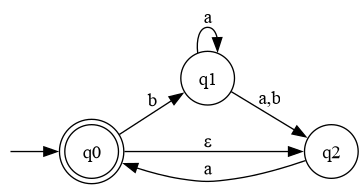
\includegraphics[width=0.4\linewidth,height=\textheight,keepaspectratio]{chapters/images/afn1.png}

}

\caption{\label{fig-afn1}Autômato Finito Não-Determinístico}

\end{figure}%

\subsubsection{Computação em um AFN}\label{computauxe7uxe3o-em-um-afn}

A computação de um Autômato Finito Não Determinístico (AFN) consiste em
acompanhar os possíveis estados em que o autômato pode se encontrar à
medida que os símbolos da cadeia de entrada são processados.
Diferentemente de um AFD, para um determinado estado e símbolo pode
existir mais de um estado possível para o próximo passo. Além disso, o
AFN pode realizar transições espontâneas, representadas por
\(\varepsilon\), sem consumir nenhum símbolo da cadeia de entrada.

Considere o AFN apresentado anteriormente, cuja tabela de transição é:

\begin{longtable*}[]{|c|c|c|c|}
\toprule\noalign{}
Estado & \(a\) & \(b\) & \(\varepsilon\) \\
\midrule\noalign{}
\endhead
\bottomrule\noalign{}
\endlastfoot
\(q_0\) & \(\varnothing\) & \(\{q_1\}\) & \(\{q_2\}\) \\
\midrule
\(q_1\) & \(\{q_1,q_2\}\) & \(\{q_2\}\) & \(\varnothing\) \\
\midrule
\(q_2\) & \(\{q_0\}\) & \(\varnothing\) & \(\varnothing\) \\
\end{longtable*}

O estado \(q_0\) é o estado inicial e também é um estado final.

Observe, por exemplo, que

\[
\delta(q_1,a)=\{q_1,q_2\}.
\]

Isso significa que, estando em \(q_1\) e lendo o símbolo \(a\), o
autômato pode permanecer em \(q_1\) ou pode ir para \(q_2\). Essa
possibilidade de escolha caracteriza o comportamento não determinístico
do AFN.

Além disso,

\[
\delta(q_0,\varepsilon)=\{q_2\},
\]

o que significa que o autômato pode passar de \(q_0\) para \(q_2\) sem
consumir nenhum símbolo da entrada.

\subsubsection{Exemplo de computação}\label{exemplo-de-computauxe7uxe3o}

Considere a cadeia

\[
w=bba.
\]

Vamos acompanhar uma possível computação do AFN.

Inicialmente, o autômato encontra-se em \(q_0\). Como existe uma
transição \(\varepsilon\) de \(q_0\) para \(q_2\), antes mesmo de
consumir qualquer símbolo o autômato também pode estar em \(q_2\).
Portanto, a \(\varepsilon\)-fecho do estado inicial é

\[
\varepsilon\text{-fecho}(q_0)=\{q_0,q_2\}.
\]

Agora, o primeiro símbolo da cadeia é \(b\). A partir dos estados
\(\{q_0,q_2\}\), temos:

\[
\delta(q_0,b)=\{q_1\}
\]

e

\[
\delta(q_2,b)=\varnothing.
\]

Logo, após consumir o primeiro símbolo \(b\), o conjunto de estados
possíveis é

\[
\{q_1\}.
\]

O segundo símbolo também é \(b\). Como

\[
\delta(q_1,b)=\{q_2\},
\]

temos:

\[
\{q_1\}
\xrightarrow{b}
\{q_2\}.
\]

Finalmente, resta consumir o símbolo \(a\). Como

\[
\delta(q_2,a)=\{q_0\},
\]

obtemos:

\[
\{q_2\}
\xrightarrow{a}
\{q_0\}.
\]

Como \(q_0\) é um estado final, a cadeia \(bba\) é aceita pelo AFN.

Podemos representar essa computação por:

\[
q_0
\xrightarrow{b}
q_1
\xrightarrow{b}
q_2
\xrightarrow{a}
q_0.
\]

Como a computação termina em um estado final, concluímos que

\[
bba \in L(M),
\]

onde \(L(M)\) representa a linguagem reconhecida pelo autômato \(M\).

As múltiplas computações possíveis no AFN também podem ser representada
numa árvore:

\begin{figure}

\centering{

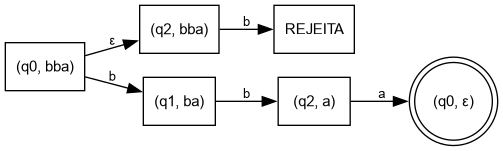
\includegraphics[width=0.6\linewidth,height=\textheight,keepaspectratio]{chapters/images/computa-afn.png}

}

\caption{\label{fig-computa-anf}Múltiplas computações do AFN}

\end{figure}%

\subsubsection{Não determinismo e múltiplas
computações}\label{nuxe3o-determinismo-e-muxfaltiplas-computauxe7uxf5es}

Uma característica importante do AFN é que uma mesma cadeia pode
produzir diferentes caminhos de computação. Considere, por exemplo, o
estado \(q_1\) e o símbolo \(a\):

\[
\delta(q_1,a)=\{q_1,q_2\}.
\]

Assim, ao ler \(a\) em \(q_1\), existem duas possibilidades:

\[
q_1\xrightarrow{a}q_1
\qquad\text{ou}\qquad
q_1\xrightarrow{a}q_2.
\]

Portanto, uma cadeia é aceita por um AFN quando \textbf{existe pelo
menos uma computação que consome toda a cadeia e termina em um estado
final}.

Não é necessário que todas as possíveis computações terminem em estados
finais. Basta que uma delas seja bem-sucedida.

\subsubsection{A função de transição e as transições
inexistentes}\label{a-funuxe7uxe3o-de-transiuxe7uxe3o-e-as-transiuxe7uxf5es-inexistentes}

Na representação gráfica de um AFN, normalmente desenhamos apenas as
transições que realmente existem. Por exemplo, não há no autômato uma
transição de \(q_0\) com o símbolo \(a\). Por isso, na tabela aparece:

\[
\delta(q_0,a)=\varnothing.
\]

De maneira semelhante,

\[
\delta(q_2,b)=\varnothing.
\]

Isso significa que não existe uma transição possível para aquele par
estado/símbolo.

Nesse sentido, quando consideramos apenas as transições explicitamente
representadas no diagrama, podemos dizer que a função de transição é
\textbf{parcial}: alguns pares \((q,x)\) não possuem uma transição
associada.

Entretanto, existe uma importante observação formal. A função de
transição de um AFN pode ser definida como

\[
\delta:Q\times(\Sigma\cup\{\varepsilon\})
\longrightarrow\mathcal{P}(Q),
\]

onde \(\mathcal{P}(Q)\) é o conjunto das partes de \(Q\).

Nessa definição, \(\delta\) é uma função \textbf{total}, pois todo par
\((q,x)\) possui um resultado. Quando não existe uma transição, o
resultado é simplesmente o conjunto vazio:

\[
\delta(q,x)=\varnothing.
\]

Por exemplo,

\[
\delta(q_0,a)=\varnothing
\]

não significa que a função deixou de estar definida. Significa que, a
partir de \(q_0\), não existe nenhum estado possível ao consumir \(a\).

Assim, é possível adotar duas formas de interpretação:

\begin{itemize}
\tightlist
\item
  \textbf{representação gráfica:} apenas as transições existentes são
  representadas, podendo-se dizer que a relação de transição é parcial;
\item
  \textbf{definição formal:} a função \(\delta\) é total e retorna
  \(\varnothing\) para os pares para os quais não existe uma transição.
\end{itemize}

Essa segunda definição é particularmente conveniente porque permite
tratar uniformemente todos os pares estado/símbolo e será utilizada na
construção de algoritmos para AFNs e na conversão de AFNs em AFDs.

\subsection{Expressões Regulares}\label{expressuxf5es-regulares}

Um outro formalismo que pode ser utilizado para definição de linguagens
são as Expressões Regulares (ER). Assim como as expressões aritméticas
tem operadores (soma, multiplicação, divisão, \ldots) que são utilizados
para expressar valores numéricos, as \textbf{expressões regulares} usam
os operadores de concatenação, união (representado pelo símbolo +) e
fecho de Kleene (representado pelo símbolo *) para definir linguagens
regulares.

\begin{definition}[]\protect\hypertarget{def-operacoes-regulares}{}\label{def-operacoes-regulares}

Sejam \(A\) e \(B\) linguagens. As operações regulares de União,
Concatenação e Fecho de Kleene são definidas da seguinte forma:

\begin{itemize}
\item
  União: \(A \cup B = \{x | x \in A\) ou \(x \in B\}\).
\item
  Concatenação: \(AB = \{xy | x \in A\) e \(y \in B\}\).
\item
  Fecho de Kleene: \(A^*= \{x_1x_2...x_k | k \geq 0\) e \(x_i \in A\}\).
\end{itemize}

\end{definition}

\begin{definition}[]\protect\hypertarget{def-expressao-regular}{}\label{def-expressao-regular}

Uma ER sobre uma alfabeto \(\Sigma\) é definida recursivamente como:

\begin{enumerate}
\def\labelenumi{\arabic{enumi}.}
\item
  \(\emptyset\), \(\lambda\) e \(a\) para qualquer \(a \in \Sigma\) são
  expressões regulares; tais que ER's denotam, respectivamente, os
  conjuntos \(\emptyset\), \(\{\lambda\}\) e \(\{a\}\)
\item
  Se \(r\) e \(s\) são expressões regulares, então também são expressões
  regulares \((r+s)\), \((rs)\) e \(r^*\); tais ER's denotam,
  respectivamente, \(L(r) \cup L(s)\), \(L(r)L(s)\) e \(L(r)^*\).
\end{enumerate}

\end{definition}

Alguns exemplos de ER considerando o alfabeto \(\Sigma = \{a, b\}\):

\begin{enumerate}
\def\labelenumi{\arabic{enumi}.}
\item
  a*ba* = \{\(w \in \Sigma^* | w\) contém um único b\}
\item
  (a + \(\lambda\))b = \{\(w \in \Sigma^* | w\) começa com a ou nada
  seguido de b\}
\item
  a*b = \{\(w \in \Sigma^* | w\) contém zero ou mais a´s finalizado por
  b\}
\item
  a(a+b)*a+a = \{\(w \in \Sigma^* | w\) começa e termina com a\}
\end{enumerate}

\subsection{Conversão de ER para AFN}\label{conversuxe3o-de-er-para-afn}

\begin{theorem}[]\protect\hypertarget{thm-fecho-regular}{}\label{thm-fecho-regular}

A classe de Linguagens Regulares é fechada com relação as operações de
União, Concatenação e fecho de Kleene.

\end{theorem}

A construção de autômatos finitos não determinísticos (AFNs) a partir de
expressões regulares pode ser realizada de forma incremental, combinando
autômatos menores por meio de operações sobre linguagens. Neste
processo, cada operação é representada por uma estrutura de estados e
transições que permite construir um AFN equivalente à expressão regular
considerada (Sipser, 2012; Vieira, 2006).

Considere que \(A\) e \(B\) são AFNs que reconhecem, respectivamente, as
linguagens \(L(A)\) e \(L(B)\). As construções apresentadas permitem
obter novos autômatos que reconhecem a união, a concatenação e o fecho
de Kleene dessas linguagens.

\subsubsection{Operação de união}\label{operauxe7uxe3o-de-uniuxe3o}

A operação de união entre duas linguagens \(L(A)\) e \(L(B)\) produz uma
linguagem que contém todas as palavras reconhecidas por pelo menos um
dos dois autômatos. Sua definição é:

\[
L(A)\cup L(B)=\{w\mid w\in L(A)\text{ ou }w\in L(B)\}
\]

Para construir um AFN que reconheça essa linguagem, são criados um novo
estado inicial \(q_i\) e um novo estado final \(q_f\). O novo estado
inicial é conectado, por transições \(\varepsilon\), aos estados
iniciais dos autômatos \(A\) e \(B\). Dessa forma, o processamento pode
começar em qualquer um dos dois autômatos, sem consumir símbolos da
entrada.

Em seguida, todos os estados finais originais de \(A\) e \(B\) deixam de
ser finais e recebem transições \(\varepsilon\) para o novo estado final
\(q_f\). Assim, quando o processamento de qualquer um dos autômatos
alcança um de seus estados finais originais, ele pode realizar uma
transição vazia para o novo estado final.

O novo estado final passa a ser o único estado final do autômato
resultante. Portanto, uma palavra será aceita se puder ser reconhecida
integralmente pelo autômato \(A\) ou pelo autômato \(B\).

A demonstração da construção de AFNs para união está ilustrado na
Figura~\ref{fig-uniao-vieira}.

\begin{figure}

\centering{

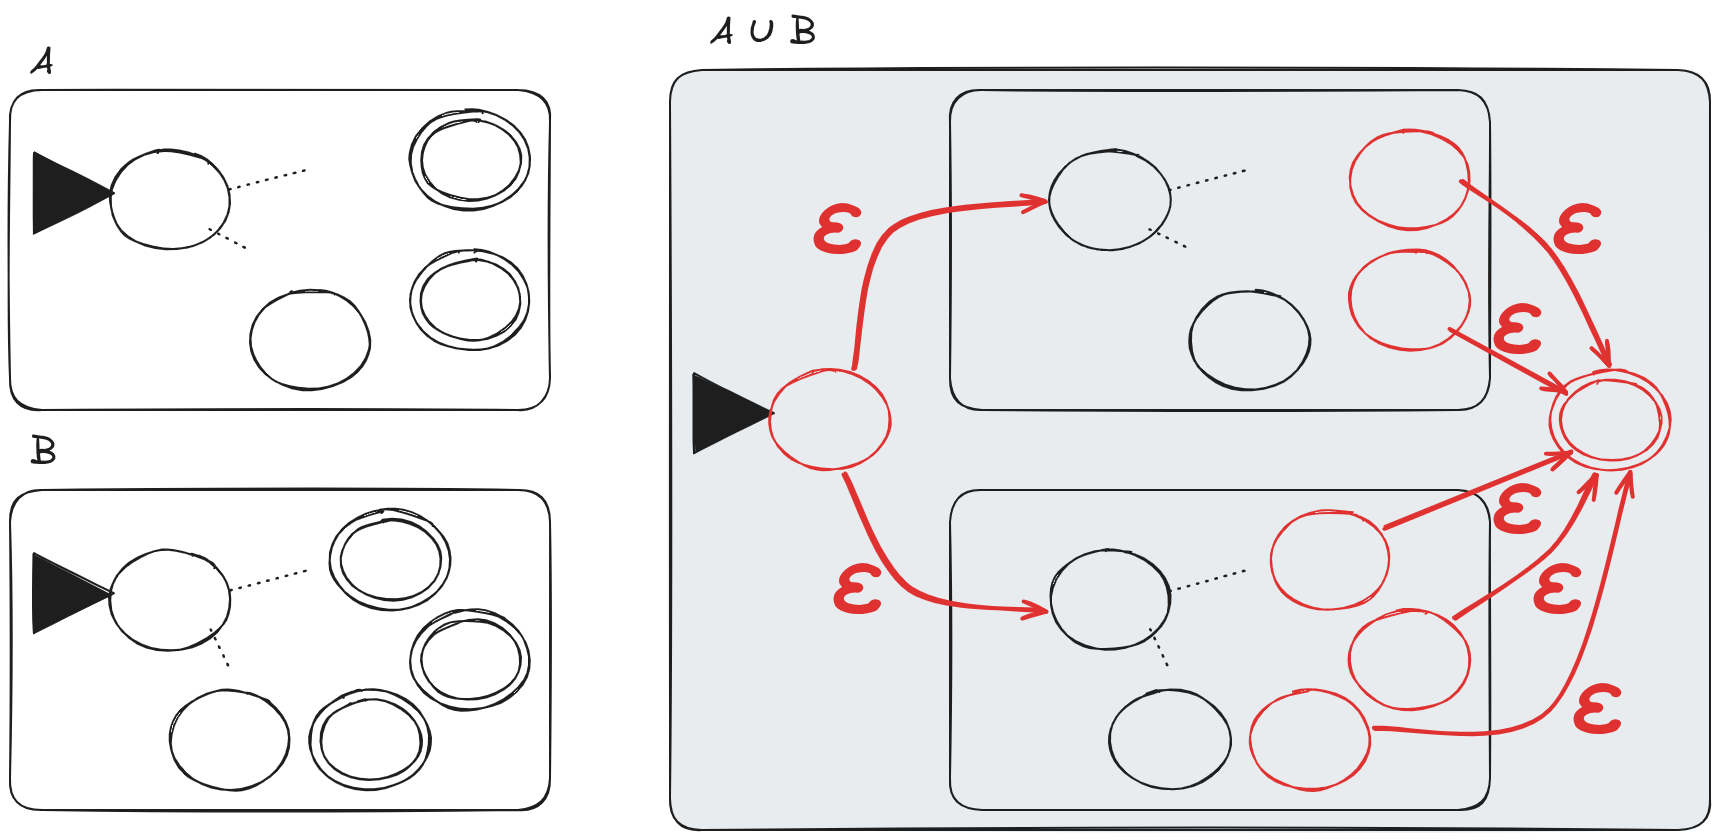
\includegraphics[width=0.6\linewidth,height=\textheight,keepaspectratio]{chapters/images/uniao-vieira.png}

}

\caption{\label{fig-uniao-vieira}Construção de uma AFN \(A\) para
reconhecer \(A \cup B\)}

\end{figure}%

\subsubsection{Operação de
concatenação}\label{operauxe7uxe3o-de-concatenauxe7uxe3o}

A concatenação de duas linguagens \(L(A)\) e \(L(B)\) corresponde ao
conjunto de palavras que podem ser formadas pela justaposição de uma
palavra de \(L(A)\) com uma palavra de \(L(B)\). Formalmente:

\[
L(A)L(B)=\{xy\mid x\in L(A)\text{ e }y\in L(B)\}
\]

Para construir o AFN correspondente, são criados um novo estado inicial
\(q_i\) e um novo estado final \(q_f\). O novo estado inicial é
conectado ao estado inicial de \(A\) por uma transição \(\varepsilon\).
Essa transição permite iniciar o processamento de \(A\) sem consumir
nenhum símbolo da entrada.

Todos os estados finais originais de \(A\) deixam de ser finais e são
conectados, por transições \(\varepsilon\), ao estado inicial de \(B\).
Essas transições permitem que, após reconhecer uma palavra pertencente a
\(L(A)\), o processamento continue em \(B\), sem consumir símbolos
adicionais.

Por fim, todos os estados finais originais de \(B\) deixam de ser finais
e são conectados ao novo estado final \(q_f\) por transições
\(\varepsilon\). O novo estado final passa a ser o único estado final do
autômato resultante.

Dessa maneira, uma palavra será aceita somente se puder ser dividida em
duas partes: a primeira reconhecida por \(A\) e a segunda reconhecida
por \(B\), respeitando a ordem da concatenação.

A demonstração da construção de AFNs para concatenação está ilustrado na
Figura~\ref{fig-concatena-vieira}.

\begin{figure}

\centering{

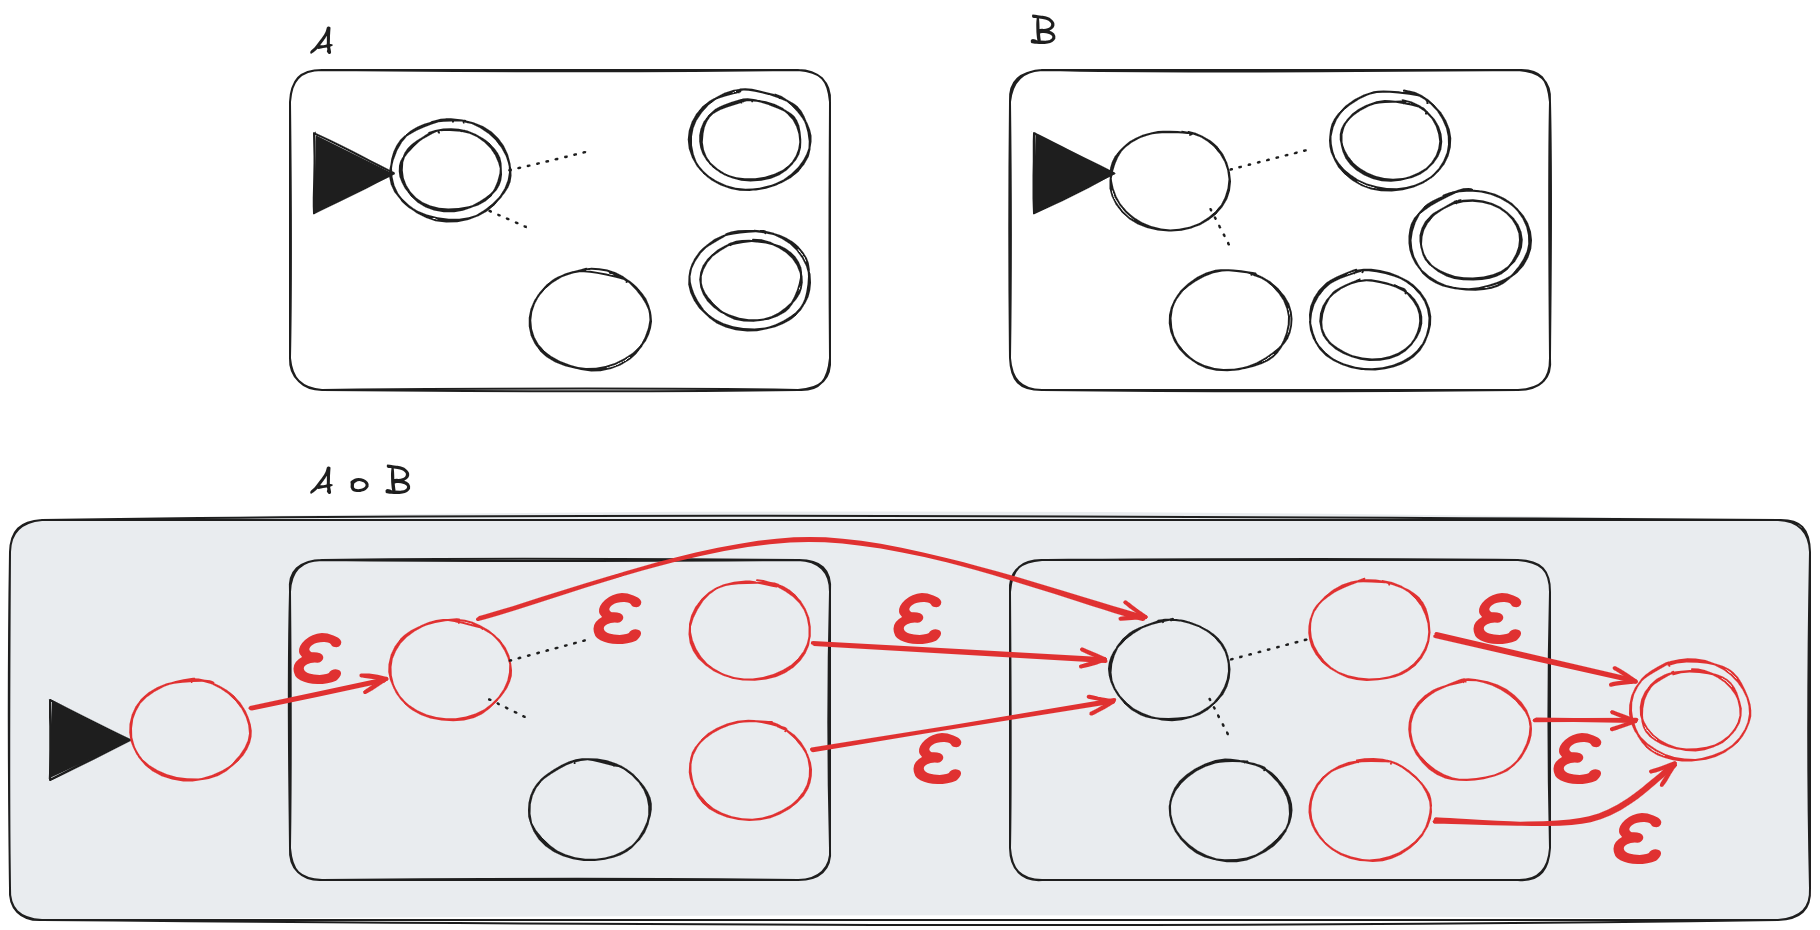
\includegraphics[width=0.6\linewidth,height=\textheight,keepaspectratio]{chapters/images/concatena-vieira.png}

}

\caption{\label{fig-concatena-vieira}Construção de uma AFN \(A\) para
reconhecer \(AB\)}

\end{figure}%

\subsubsection{Fecho de Kleene}\label{fecho-de-kleene}

O fecho de Kleene de uma linguagem \(L(A)\) corresponde ao conjunto de
todas as concatenações de zero ou mais palavras pertencentes a essa
linguagem. Sua definição é:

\[
L(A)^*=\bigcup_{n\geq 0}L(A)^n
\]

Em particular, a linguagem resultante sempre contém a palavra vazia
\(\varepsilon\), correspondente à concatenação de zero palavras.

Para construir o AFN correspondente, são criados um novo estado inicial
\(q_i\) e um novo estado final \(q_f\). O novo estado inicial é
conectado ao estado inicial de \(A\) por uma transição \(\varepsilon\),
permitindo iniciar o reconhecimento de uma palavra pertencente a
\(L(A)\).

Além disso, o novo estado inicial é conectado diretamente ao novo estado
final por uma transição \(\varepsilon\). Essa ligação permite aceitar a
palavra vazia, sem executar o autômato \(A\).

Todos os estados finais originais de \(A\) deixam de ser finais e
recebem transições \(\varepsilon\) para o novo estado final \(q_f\).
Dessa forma, o processamento pode terminar após reconhecer uma palavra
de \(L(A)\).

Para permitir a repetição, o novo estado final também é conectado ao
novo estado inicial por uma transição \(\varepsilon\). Essa ligação
possibilita retornar ao início da construção e processar outra
ocorrência de uma palavra de \(L(A)\). Assim, o autômato pode reconhecer
zero, uma ou várias ocorrências de palavras da linguagem original.

O novo estado final passa a ser o único estado final do autômato
resultante. A combinação dessas transições garante que o AFN reconheça
exatamente o fecho de Kleene da linguagem original.

A demonstração da construção de AFNs para a operação de fecho de Kleene
está ilustrado na Figura~\ref{fig-kleene-vieira}.

\begin{figure}

\centering{

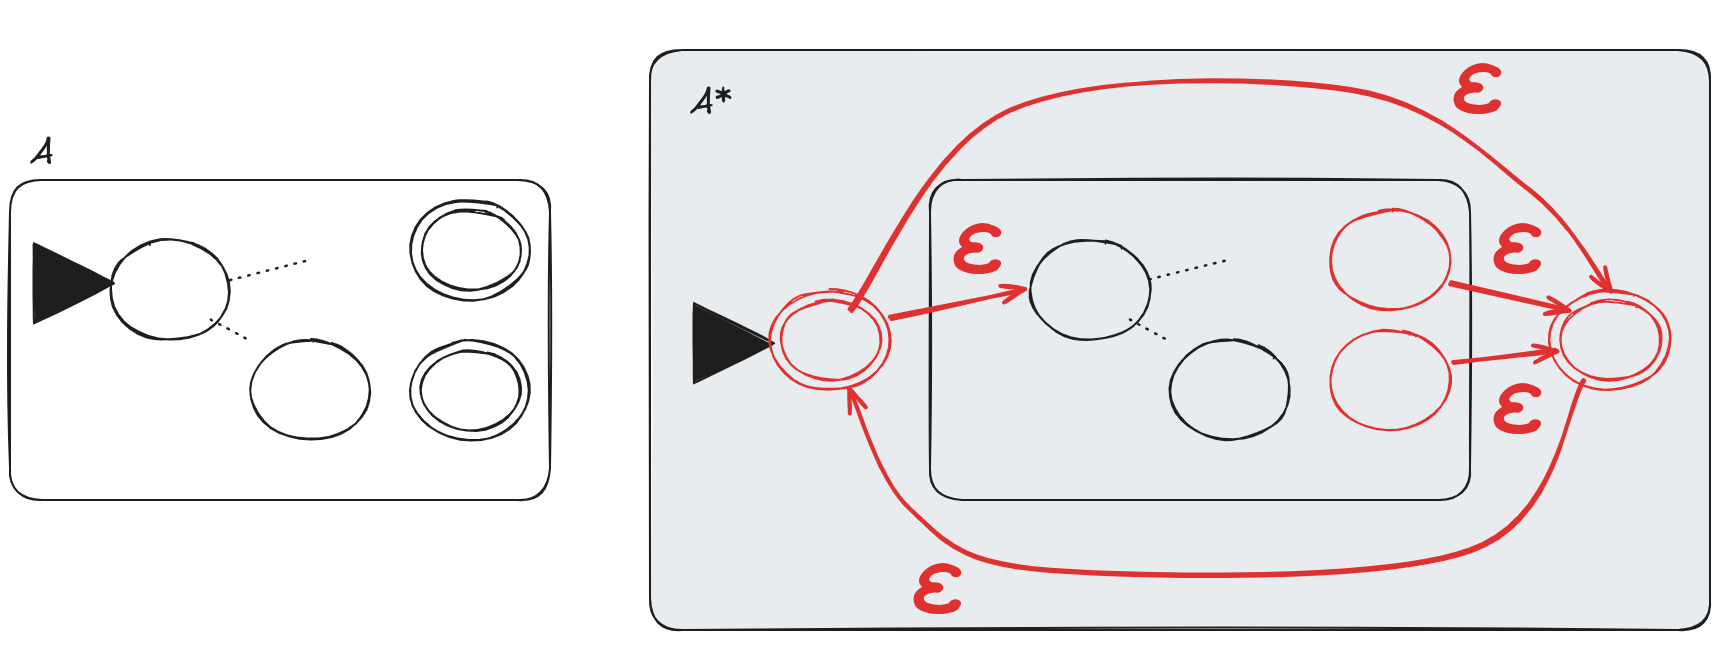
\includegraphics[width=0.6\linewidth,height=\textheight,keepaspectratio]{chapters/images/kleene-vieira.png}

}

\caption{\label{fig-kleene-vieira}Construção de uma AFN \(A\) para
reconhecer \(A^*\)}

\end{figure}%

\subsubsection{Construção de AFNs pelo método de
Thompson}\label{construuxe7uxe3o-de-afns-pelo-muxe9todo-de-thompson}

O método de Thompson permite traduzir sistematicamente uma expressão
regular em um autômato finito não determinístico (AFN). A ideia central
é construir autômatos para expressões menores e combiná-los de acordo
com as operações presentes na expressão regular.

Nesta abordagem, as operações de união, concatenação e fecho de Kleene
são implementadas por meio de transições \(\varepsilon\) e, quando
necessário, pela criação de novos estados. Uma transição \(\varepsilon\)
permite passar de um estado a outro sem consumir nenhum símbolo da
palavra de entrada.

Considere que \(A\) e \(B\) são AFNs que reconhecem as linguagens
\(L(A)\) e \(L(B)\), respectivamente. A seguir, são apresentadas as
regras para construir os autômatos correspondentes às operações de
união, concatenação e fecho de Kleene.

\subsubsection{União de duas
linguagens}\label{uniuxe3o-de-duas-linguagens}

Para construir um AFN que reconheça essa linguagem, cria-se um novo
estado inicial \(q_i\). Esse estado é conectado, por transições
\(\varepsilon\), aos estados iniciais de \(A\) e \(B\).

Os estados finais dos dois autômatos são preservados como estados
finais. Não é necessário criar um novo estado final, pois o autômato
resultante aceita uma palavra quando o processamento alcança um estado
final de qualquer um dos dois autômatos originais.

A partir do novo estado inicial, o AFN pode escolher, de maneira não
determinística, entre iniciar o processamento em \(A\) ou em \(B\). Como
as transições que realizam essa escolha são transições \(\varepsilon\),
nenhum símbolo da entrada é consumido nessa etapa.

A demonstração da construção de AFNs para a operação de união está
ilustrado na Figura~\ref{fig-uniao-sipser}.

\begin{figure}

\centering{

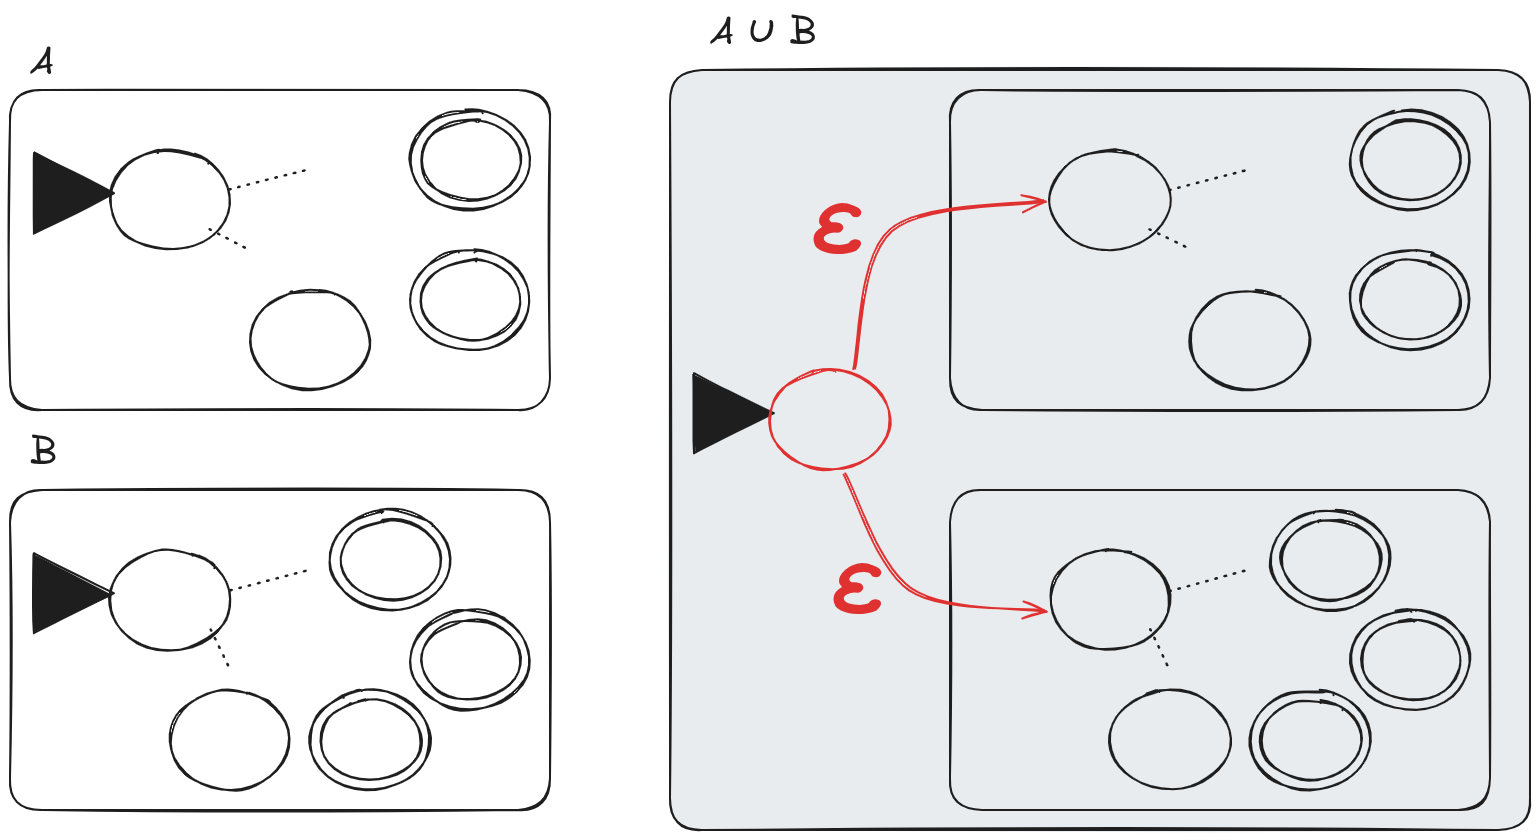
\includegraphics[width=0.6\linewidth,height=\textheight,keepaspectratio]{chapters/images/uniao-sipser.png}

}

\caption{\label{fig-uniao-sipser}Construção de uma AFN \(A\) para
reconhecer \(A \cup B\)}

\end{figure}%

\subsubsection{Concatenação de duas
linguagens}\label{concatenauxe7uxe3o-de-duas-linguagens}

Para construir o AFN correspondente à concatenação, não é necessário
criar novos estados. A construção é realizada conectando os estados
finais de \(A\) ao estado inicial de \(B\).

Cada estado final de \(A\) recebe uma transição \(\varepsilon\) para o
estado inicial de \(B\) e deixa de ser final. Os estados finais de \(B\)
permanecem finais no autômato resultante.

Essas transições permitem que o processamento, após reconhecer uma
palavra pertencente a \(L(A)\), continue pelo autômato \(B\) sem
consumir nenhum símbolo adicional. Como os estados finais de \(A\)
deixam de ser finais, a aceitação somente ocorre quando o processamento
alcança um estado final de \(B\).

O estado inicial do autômato resultante é o estado inicial de \(A\),
enquanto os estados finais são aqueles que já eram finais em \(B\).
Dessa forma, o autômato reconhece as palavras que podem ser divididas em
duas partes consecutivas: uma reconhecida por \(A\) e outra reconhecida
por \(B\).

A demonstração da construção de AFNs para a operação de concatenação
está ilustrado na Figura~\ref{fig-concatena-sipser}.

\begin{figure}

\centering{

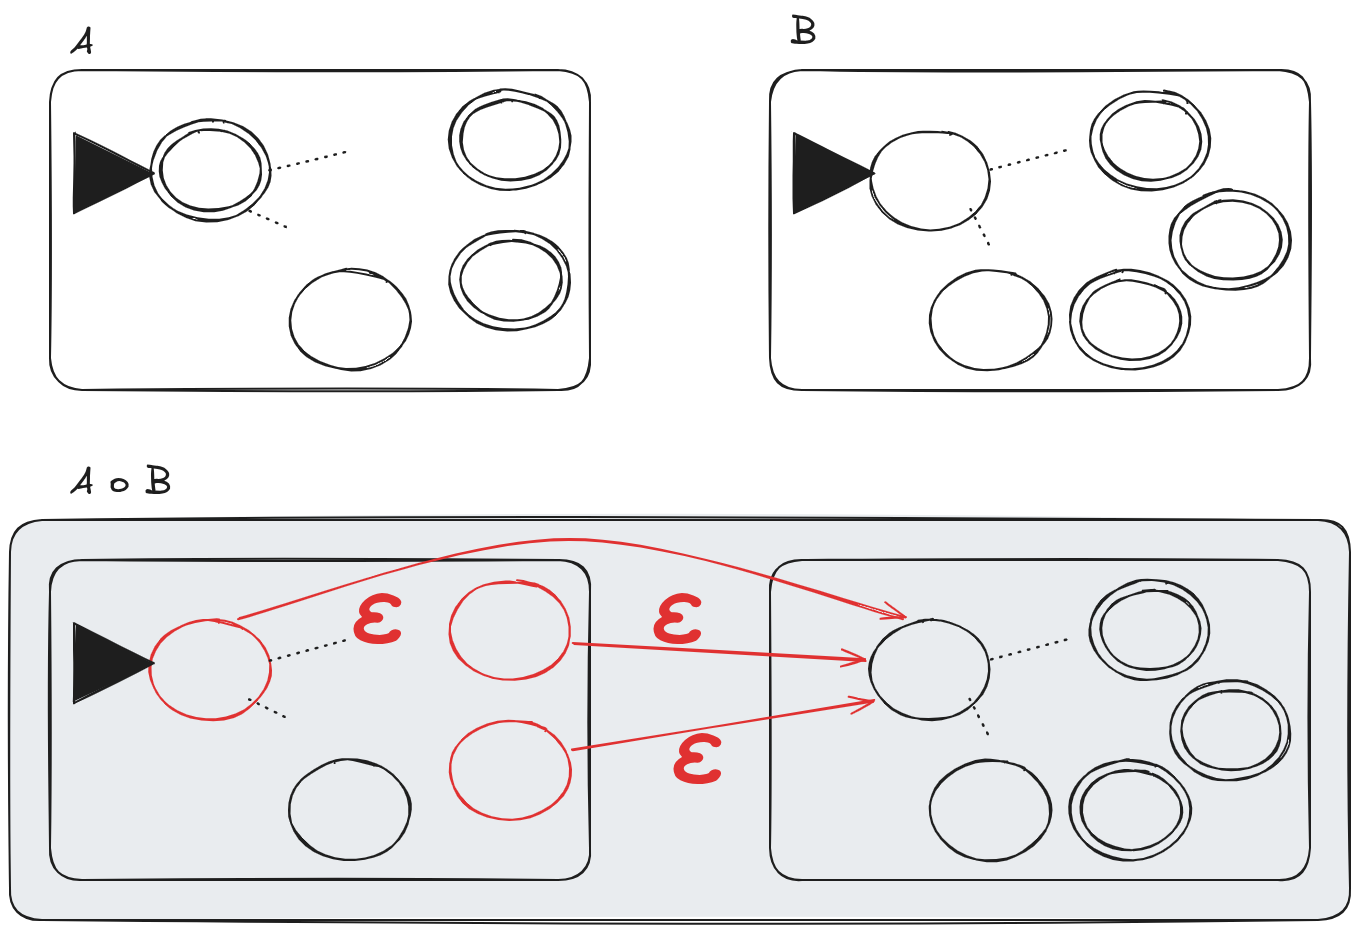
\includegraphics[width=0.6\linewidth,height=\textheight,keepaspectratio]{chapters/images/concatena-sipser.png}

}

\caption{\label{fig-concatena-sipser}Construção de uma AFN \(A\) para
reconhecer \(AB\)}

\end{figure}%

\subsubsection{Fecho de Kleene}\label{fecho-de-kleene-1}

Para construir o AFN que reconhece \(L(A)^*\), cria-se um novo estado
\(q_i\) que será simultaneamente inicial e final. O novo estado é
conectado, por uma transição \(\varepsilon\), ao estado inicial do
autômato \(A\).

O fato de \(q_i\) ser final permite aceitar imediatamente a palavra
vazia, sem percorrer nenhuma transição do autômato original.

Além disso, cada estado final de \(A\) recebe uma transição
\(\varepsilon\) de volta ao estado inicial de \(A\). Essas transições
permitem reiniciar o processamento do autômato original, possibilitando
o reconhecimento de novas ocorrências de palavras pertencentes a
\(L(A)\).

Os estados que já eram finais em \(A\) permanecem finais. Assim, após
reconhecer uma palavra de \(L(A)\), o processamento pode terminar em um
desses estados ou continuar para reconhecer outra ocorrência da
linguagem. O novo estado inicial também permanece final, garantindo a
aceitação de zero ocorrências.

A demonstração da construção de AFNs para a operação de fecho de Kleene
está ilustrado na Figura~\ref{fig-kleene-sipser}.

\begin{figure}

\centering{

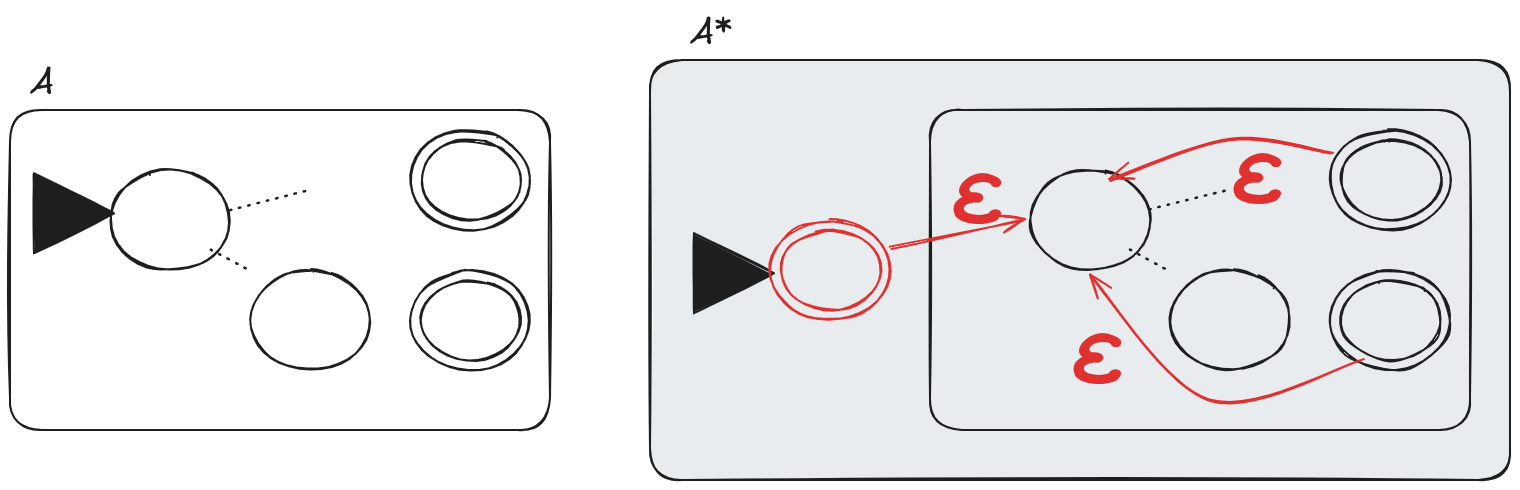
\includegraphics[width=0.6\linewidth,height=\textheight,keepaspectratio]{chapters/images/kleene-sipser.png}

}

\caption{\label{fig-kleene-sipser}Construção de uma AFN \(A\) para
reconhecer \(A^*\)}

\end{figure}%

\subsubsection{Resumo das operações}\label{resumo-das-operauxe7uxf5es}

\begin{longtable*}[]{|
  >{\raggedright\arraybackslash}p{(\linewidth - 6\tabcolsep - 4\arrayrulewidth) * \real{0.3333}}|
  >{\raggedright\arraybackslash}p{(\linewidth - 6\tabcolsep - 4\arrayrulewidth) * \real{0.3333}}|
  >{\raggedright\arraybackslash}p{(\linewidth - 6\tabcolsep - 4\arrayrulewidth) * \real{0.3333}}|}
\toprule\noalign{}
\begin{minipage}[b]{\linewidth}\smallskip
\raggedright
Operação
\end{minipage} & \begin{minipage}[b]{\linewidth}\raggedright
Modificações no AFN
\end{minipage} & \begin{minipage}[b]{\linewidth}\raggedright
Estados finais do resultado
\end{minipage} \\
\midrule\noalign{}
\endhead
\bottomrule\noalign{}
\endlastfoot
União \(A\cup B\) & Cria um novo estado inicial, conectado por
\(\varepsilon\) aos estados iniciais de \(A\) e \(B\). & Os estados
finais de \(A\) e \(B\) permanecem finais. \\
\midrule
Concatenação \(AB\) & Cada estado final de \(A\) recebe uma transição
\(\varepsilon\) para o estado inicial de \(B\) e deixa de ser final. &
Os estados finais de \(B\) permanecem finais. \\
\midrule
Fecho de Kleene \(A^*\) & Cria um novo estado inicial e final; adiciona
uma transição \(\varepsilon\) para o início de \(A\) e transições de
retorno dos finais de \(A\) ao início de \(A\). & Os estados finais de
\(A\) permanecem finais, e o novo estado também é final. \\
\end{longtable*}

\subsection{Conversão de AFN para
AFD}\label{conversuxe3o-de-afn-para-afd}

\begin{theorem}[]\protect\hypertarget{thm-afn-afd}{}\label{thm-afn-afd}

Para todo Autômato Finito Não-Determinístico existe um Autômato Finito
Determinístico correspondente.

\end{theorem}

A demonstração pode ser realizada através da simulação da execução em
paralelo da computação do AFN (Lewis; Papadimitriou, 2004; Sipser, 2012;
Vieira, 2006).

Basicamente, ao invés de mudar para um único estado a cada transição, no
AFN poderemos nos deslocar para um conjunto de estados possíveis, dada o
não-determinismo de algumas transições.

Como visto anteriormente, um conjunto com \(k\) elementos possui \(2^k\)
subconjuntos. Assim, para um conjunto de estados

\[
Q=\{1,2,3\},
\]

o conjunto das partes de \(Q\), denotado por \(\mathcal{P}(Q)\), é

\[
\mathcal{P}(Q)=
\{\emptyset,\{1\},\{2\},\{3\},\{1,2\},\{1,3\},\{2,3\},\{1,2,3\}\}.
\]

Na construção de um AFD equivalente a um AFN, cada estado do AFD
representa um \textbf{conjunto de estados do AFN}. Portanto, se o AFN
possui \(k\) estados, o AFD resultante poderá possuir, no máximo,
\(2^k\) estados, correspondentes aos elementos de \(\mathcal{P}(Q)\).

Embora esse número possa parecer elevado, na prática nem todos os
subconjuntos de \(Q\) precisam ser alcançados durante a construção do
AFD. Além disso, durante a simulação de uma cadeia de entrada, apenas os
conjuntos de estados efetivamente alcançáveis são considerados.

\subsubsection{\texorpdfstring{\(\varepsilon\)-fecho}{\textbackslash varepsilon-fecho}}\label{varepsilon-fecho}

As transições \(\varepsilon\) permitem que um AFN mude de estado sem
consumir um símbolo da cadeia de entrada. Para determinar todos os
estados que podem ser alcançados dessa maneira, utiliza-se o conceito de
\textbf{\(\varepsilon\)-fecho}.

Seja

\[
M=(Q,\Sigma,\delta,q_0,F)
\]

um AFN, em que a função de transição é dada por

\[
\delta:Q\times(\Sigma\cup\{\varepsilon\})\rightarrow\mathcal{P}(Q).
\]

Para um estado \(q\in Q\), define-se o \textbf{\(\varepsilon\)-fecho de
\(q\)} como o conjunto de estados que podem ser alcançados a partir de
\(q\) utilizando \textbf{zero ou mais transições \(\varepsilon\)}:

\[
\varepsilon\text{-fecho}(q)
=
\{p\in Q\mid q\overset{\varepsilon^*}{\longrightarrow}p\}.
\]

O uso de \textbf{zero ou mais} transições é importante: o próprio estado
\(q\) pertence ao seu \(\varepsilon\)-fecho, pois é possível permanecer
em \(q\) sem realizar nenhuma transição.

De forma mais geral, para um conjunto de estados \(R\subseteq Q\),
define-se:

\[
\varepsilon\text{-fecho}(R)
=
\bigcup_{q\in R}\varepsilon\text{-fecho}(q).
\]

Equivalentemente,

\[
\varepsilon\text{-fecho}(R)
=
\{p\in Q\mid
\exists q\in R\text{ tal que }
q\overset{\varepsilon^*}{\longrightarrow}p
\}.
\]

Portanto, o \(\varepsilon\)-fecho de um conjunto \(R\) contém todos os
estados que podem ser alcançados a partir de \textbf{qualquer estado de
\(R\)}, utilizando apenas transições \(\varepsilon\), incluindo os
próprios estados de \(R\).

Esse conceito é fundamental na construção do AFD equivalente a um AFN,
pois, ao processar um símbolo da entrada, é necessário considerar não
apenas os estados alcançados diretamente pelo símbolo, mas também todos
os estados que podem ser alcançados posteriormente por meio de
transições \(\varepsilon\).

Através de \(P(Q)\) e \(\varepsilon\text{-fecho}(R)\) podemos construir
o AFD \(M = \{Q', \Sigma, \delta', i', F'\}\) equivalente ao AFN
\(N = \{Q, \Sigma, \delta, i, F\}\) da seguinte forma:

\begin{itemize}
\item
  \(Q' \subseteq P(Q)\).
\item
  Para \(R \in Q'\),
  \(\delta'(R,a) = \bigcup_{r \in R}\varepsilon\text{-fecho}(\delta(r,a))\)
\item
  \(i = \varepsilon\text{-fecho}(\{i\})\).
\item
  \(F' = \{R \in Q' | R\) contém um estado de aceitação do \(AFN \}\)
\end{itemize}

\subsubsection{Exemplo de conversão de uma expressão regular para um AFD
correspondente}\label{exemplo-de-conversuxe3o-de-uma-expressuxe3o-regular-para-um-afd-correspondente}

Para exemplificar todo o processo de conversão de uma expressão regular
para um autômato finito não-determinístico e desse para um autômato
finito determinístico, faremos uma tradução para \(ER = 0^*1+0\):

\begin{enumerate}
\def\labelenumi{\arabic{enumi}.}
\item
  A tradução da \(ER = 0\) para o AFN está representada
  Figura~\ref{fig-zero};

  \begin{figure}

  \centering{

  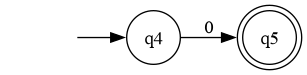
\includegraphics[width=0.35\linewidth,height=\textheight,keepaspectratio]{chapters/images/afn-zero.png}

  }

  \caption{\label{fig-zero}AFN correspondente a \(ER = 0\)}

  \end{figure}%
\item
  A tradução da \(ER = 1\) para o AFN está representada na
  Figura~\ref{fig-um};

  \begin{figure}

  \centering{

  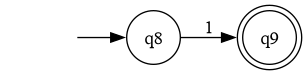
\includegraphics[width=0.4\linewidth,height=\textheight,keepaspectratio]{chapters/images/afn-um.png}

  }

  \caption{\label{fig-um}AFN correspondente a \(ER = 1\)}

  \end{figure}%
\item
  A tradução da \(ER = 0^*\) para o AFN está representada na
  Figura~\ref{fig-zeroestrela};

  \begin{figure}

  \centering{

  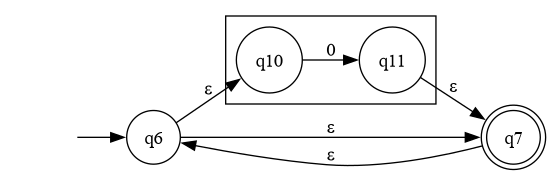
\includegraphics[width=0.6\linewidth,height=\textheight,keepaspectratio]{chapters/images/afn-zero-estrela.png}

  }

  \caption{\label{fig-zeroestrela}AFN correspondente a \(ER = 0^*\)}

  \end{figure}%
\item
  A tradução da \(ER = 0^*1\) para o AFN está representada na
  Figura~\ref{fig-zeroestrelaum};

  \begin{figure}

  \centering{

  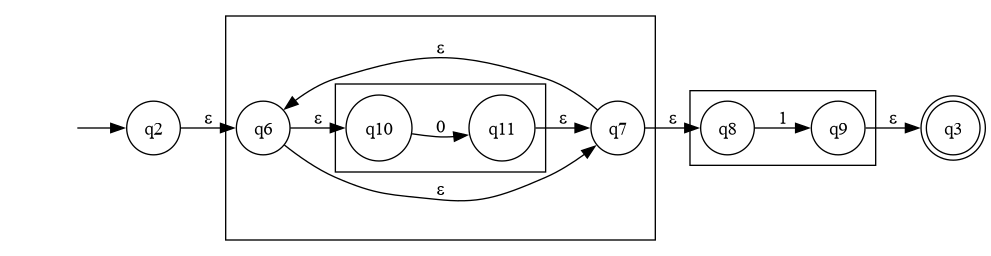
\includegraphics[width=0.8\linewidth,height=\textheight,keepaspectratio]{chapters/images/afn-zero-estrela-um.png}

  }

  \caption{\label{fig-zeroestrelaum}AFN correspondente a \(ER = 0^*1\)}

  \end{figure}%
\item
  A tradução da \(ER = 0^*1+0\) para o AFN está representada na
  Figura~\ref{fig-zeroestrelaumouzero};

  \begin{figure}

  \centering{

  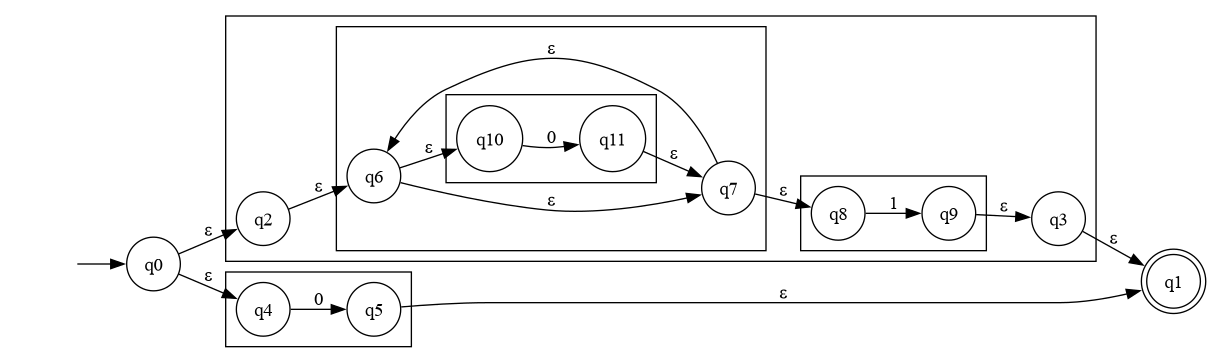
\includegraphics[width=1\linewidth,height=\textheight,keepaspectratio]{chapters/images/afn-zero-estrela-um-ou-zero.png}

  }

  \caption{\label{fig-zeroestrelaumouzero}AFN correspondente a
  \(ER = 0^*1+0\)}

  \end{figure}%
\item
  A tradução do AFN =
  \((\{q_0,q_1,q_2,q_3,q_4,q_5,q_6,q_7,q_8,q_9,q_{10},q_{11}\}, \{0,1\}, \delta,q_0,\{q_1\})\)
  da Figura~\ref{fig-zeroestrelaumouzero} para o AFD =
  \((\{q_0', q_1', q_2', q_3'\}, \{0,1\}, \delta', q_0', \{q_1', q_2'\})\)
  correspondente da Figura~\ref{fig-afd} é realizada conforme os passos
  seguintes. Primeiro o estado inicial para AFD correspondente é
  calculado como:
  \[q_0' = \varepsilon\text{-fecho}(q_0) = \{q_0, q_2, q_4, q_6, q_{10}, q_7, q_8\}\]
  A função de transição \(\delta'\) é calculada até a idempotência, da
  seguinte forma:

  \$

  \begin{array}{ll}
          \delta'(q_0', 0) =  & \bigcup_{q \in q_0'}\varepsilon\text{-fecho}(\delta(q,0)) = \\
              &  \varepsilon\text{-fecho}(\delta(q_4,0)) \cup \varepsilon\text{-fecho}(\delta(q_{10},0)) = \\
              & \{q_5, q_1\} \cup \{q_{11},q_7,q_6,q_{10},q_8\} = \\ 
              & \{q_5,q_7,q_{10},q_1,q_8,q_6,q_{11}\} = q_1'\\
          \delta'(q_0', 1) = & \bigcup_{q \in q_0'}\varepsilon\text{-fecho}(\delta(q,1)) = \\
              & \varepsilon\text{-fecho}(\delta(q_8,1)) = \\
              & \{q_9,q_3,q_1\} = q_2' \\
          \delta'(q_1', 0) = & \bigcup_{q \in q_1'}\varepsilon\text{-fecho}(\delta(q,0)) = \\
              & \varepsilon\text{-fecho}(\delta(q_{10},0))  = \\
              & \{q_{11},q_7,q_8,q_6,q_{10}\} = q_3' \\
          \delta'(q_1', 1) = & \bigcup_{q \in q_1'}\varepsilon\text{-fecho}(\delta(q,1)) = \\
              & \varepsilon\text{-fecho}(\delta(q_8,1)) = \\
              & \{q_9,q_3,q_1\} = q_2' \\
          \delta'(q_3', 0) = & \bigcup_{q \in q_3'}\varepsilon\text{-fecho}(\delta(q,0)) = \\
              & \varepsilon\text{-fecho}(\delta(q_{10},0)) = \\
              & \{q_{11},q_7,q_8,q_6,q_{10}\} = q_3' \\
          \delta'(q_3', 1) = & \bigcup_{q \in q_3'}\varepsilon\text{-fecho}(\delta(q,1)) = \\
              & \varepsilon\text{-fecho}(\delta(q_8,1)) = \\
              & \{q_9,q_3,q_1\} = q_2' \\
          \end{array}

  \$

  E o conjunto de estados finais \(F = \{q_1', q_2'\}\), pois são os
  estados do AFD que contém o estado final \(q_1\) do AFN.

  \begin{figure}

  \centering{

  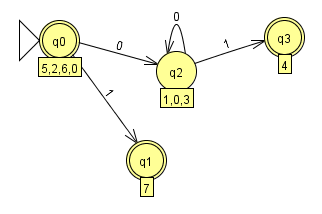
\includegraphics[width=1\linewidth,height=\textheight,keepaspectratio]{chapters/images/afd.png}

  }

  \caption{\label{fig-afd}AFD equivalente ao AFN da Figura
  Figura~\ref{fig-zeroestrelaumouzero}}

  \end{figure}%
\end{enumerate}

O resultado desse processo todo é um autômato finito determinístico
correspondente a expressão regular informada.

Todo esse processo pode ser automatizado, executado através de
ferramentas que representam essas estruturas (autômatos, expressões
regulares) e implementam os algoritmos conforme descritos. São esses
algoritmos que estão implementados em ferramentas de geração de
analisadores léxicos, como Lex e Flex. A partir de um arquivo de
especificação que contém as expressões regulares que pretende-se
reconhecer, Lex/Flex traduzem as expressões em autômatos e desse em
código em linguagem C, que implementam a programa de reconhecimento dos
lexemas.

No exemplo ilustrativo em sequência estão implementados esses
algoritmos. Você pode entrar com a expressão regular para converter para
o autômato finito não determinístico, usando as construções sugeridas
por Sipser (2012). Pode-se ainda calcular o autômato finito
determinístico e o caso mínimo deste AFD. A busca de padrões num texto
está disponível na última aba desta simulação.

\begin{figure}[H]
\centering
\fbox{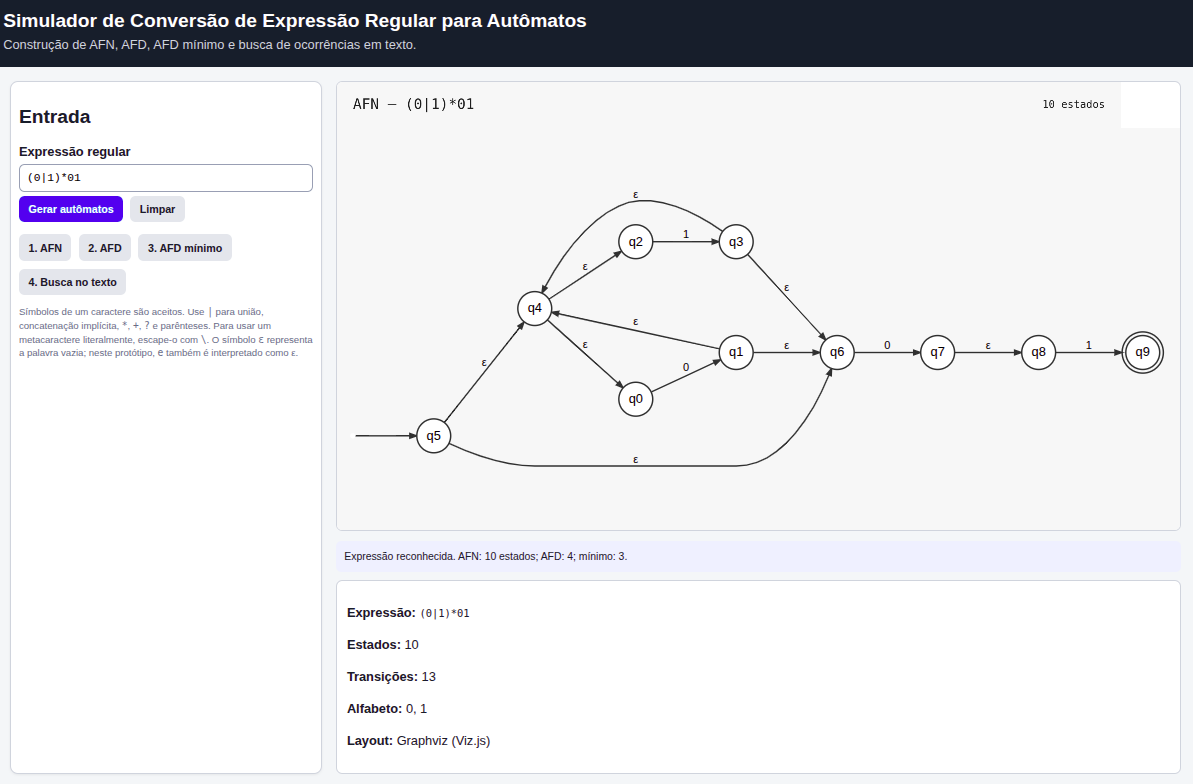
\includegraphics[width=0.6\textwidth]{chapters/images/printscreen/er-af.png}}
\caption{Visualização da aplicação interativa}
\end{figure}
\begin{tcolorbox}[enhanced jigsaw, title=Acesso Interativo]
Acesse a simulação em:\par\smallskip
\small\url{https://luizedsilva.github.io/Livro-LTC/p5js/er-af/}
\begin{center}
\includegraphics[width=3cm]{chapters/images/qrcode/er-af.png}\end{center}
\end{tcolorbox}

\section{Análise Léxica}\label{anuxe1lise-luxe9xica}

A análise léxica constitui a primeira etapa do processo de compilação e
tem como principal responsabilidade transformar o programa-fonte,
originalmente representado como uma sequência de caracteres, em uma
sequência de unidades léxicas denominadas \emph{tokens}. Para realizar
essa tarefa, o analisador léxico percorre o texto do programa,
normalmente da esquerda para a direita, identificando os diferentes
elementos que possuem significado para as etapas posteriores da
compilação. Dessa forma, a análise léxica estabelece a primeira forma de
interpretação estruturada do programa-fonte.

Os elementos reconhecidos pelo analisador léxico são denominados
\textbf{símbolos léxicos} ou \textbf{lexemas}. Entre eles encontram-se
palavras reservadas, operadores, identificadores, constantes literais,
constantes numéricas e delimitadores, entre outros elementos definidos
pela linguagem de programação. Também fazem parte do texto de entrada
elementos que, embora possam ser importantes para a organização e
documentação do programa, não necessariamente participam das demais
fases da compilação, como comentários, espaços em branco, tabulações e,
em determinadas linguagens, caracteres utilizados para formatação e
indentação.

Durante o processo de reconhecimento, o analisador léxico identifica
cada lexema e associa a ele um \emph{token}, que representa sua
categoria léxica. Por exemplo, ao encontrar a sequência de caracteres
\texttt{enquanto}, o analisador pode reconhecê-la como uma palavra
reservada e produzir um \emph{token} \texttt{T\_ENQTO}. Da mesma forma,
uma sequência de caracteres que corresponda a um identificador pode
produzir um \emph{token} \texttt{T\_IDENTIF}, enquanto uma sequência
numérica pode ser classificada como um \emph{token} correspondente a um
número inteiro ou real. O \emph{token} funciona, portanto, como uma
representação abstrata do elemento encontrado no programa-fonte,
permitindo que as etapas seguintes trabalhem com categorias léxicas em
vez de manipular diretamente cada caractere do texto.

A Figura~\ref{fig-analise-lexica} ilustra o processo de transformação
dos lexemas em tokens.

\begin{figure}

\centering{

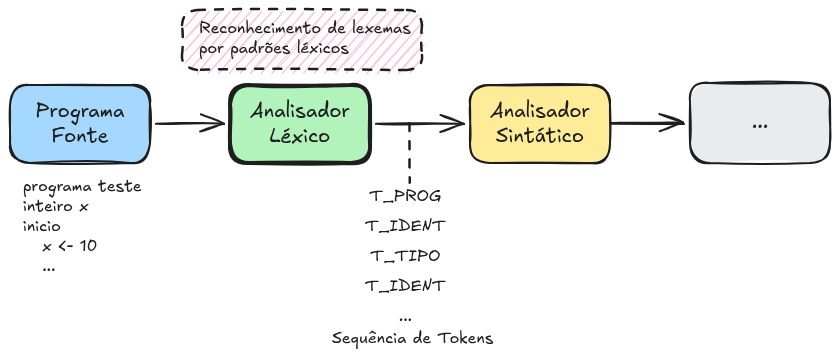
\includegraphics[width=0.8\linewidth,height=\textheight,keepaspectratio]{chapters/images/analise-lexica.png}

}

\caption{\label{fig-analise-lexica}Ilustração da fase de análise léxica}

\end{figure}%

É importante distinguir o \emph{token} do \textbf{lexema} que lhe deu
origem. O lexema corresponde à sequência concreta de caracteres
encontrada no programa-fonte, enquanto o \emph{token} representa a
categoria a que essa sequência pertence. Assim, em uma instrução como

\begin{Shaded}
\begin{Highlighting}[]
\NormalTok{soma \textless{}{-} a + }\DecValTok{10}
\end{Highlighting}
\end{Shaded}

as sequências \texttt{soma}, \texttt{a} e \texttt{10} são lexemas
encontrados no texto, enquanto seus respectivos \emph{tokens} podem ser
classificados como identificadores e constante numérica. O operador
\texttt{\textless{}-} e o operador \texttt{+} também são reconhecidos e
representados por seus respectivos \emph{tokens}. Essa separação entre a
representação concreta e sua categoria léxica simplifica o trabalho das
fases posteriores do compilador.

Nem todos os elementos encontrados durante a leitura do programa
precisam ser transformados em \emph{tokens}. Comentários, espaços em
branco e tabulações, por exemplo, normalmente são utilizados para
facilitar a leitura, a organização e a documentação do código-fonte, mas
são descartados pelo analisador léxico quando não possuem significado
para a sintaxe da linguagem. Essa regra, entretanto, depende das
características da linguagem de programação. Em algumas linguagens, como
Python por exemplo, a indentação possui significado sintático e, nesse
caso, o analisador léxico deve produzir informações que permitam às
etapas posteriores considerar as mudanças de nível de indentação.

Outro aspecto importante da análise léxica é sua interação com a
\textbf{tabela de símbolos}. Os identificadores reconhecidos pelo
analisador léxico podem estar associados a informações que serão
utilizadas durante as demais fases da compilação. Quando um
identificador é encontrado, o compilador pode verificar sua existência
na tabela de símbolos e, quando necessário, cadastrá-lo. A tabela de
símbolos mantém informações sobre entidades presentes no programa, como
identificadores de variáveis, procedimentos, funções e outros elementos
definidos pela linguagem. Embora a construção e o gerenciamento completo
dessa tabela envolvam outras fases do compilador, o reconhecimento dos
identificadores durante a análise léxica constitui uma das primeiras
oportunidades de interação com essa estrutura.

Como resultado de seu processamento, o analisador léxico produz uma
sequência de \emph{tokens} que constitui a entrada para o
\textbf{analisador sintático}. Enquanto a análise léxica procura
identificar e classificar os elementos individuais que compõem o
programa, a análise sintática utiliza a sequência de \emph{tokens} para
verificar se esses elementos estão organizados de acordo com as regras
gramaticais da linguagem. Os \emph{tokens} são, portanto, a interface
entre essas duas fases do compilador.

Considere, por exemplo, uma instrução simplificada como:

\begin{Shaded}
\begin{Highlighting}[]
\NormalTok{a \textless{}{-} b + }\DecValTok{10}
\end{Highlighting}
\end{Shaded}

O analisador léxico pode produzir uma sequência semelhante a:

\begin{Shaded}
\begin{Highlighting}[]
\NormalTok{T\_IDENTIF  T\_ATRIB  T\_IDENTIF  T\_SOMA  T\_NUMERO}
\end{Highlighting}
\end{Shaded}

A análise sintática não precisa mais trabalhar diretamente com os
caracteres \texttt{a}, \texttt{\textless{}}, \texttt{-}, \texttt{b},
\texttt{+}, \texttt{1} e \texttt{0}. Ela recebe a sequência de
\emph{tokens} e verifica se essa sequência pode ser derivada de acordo
com as produções da gramática da linguagem. Essa divisão de
responsabilidades torna o processo de compilação mais organizado e
permite que cada fase utilize mecanismos formais apropriados ao problema
que deve resolver.

Para especificar os elementos que devem ser reconhecidos na análise
léxica, utilizam-se \textbf{linguagens regulares}. Palavras reservadas,
identificadores, números, operadores e diversos outros elementos léxicos
podem ser descritos por meio de padrões regulares. As \textbf{expressões
regulares} fornecem uma notação conveniente para representar esses
padrões e constituem uma das principais formas de especificação
utilizadas na construção de analisadores léxicos.

A relação entre expressões regulares e \textbf{autômatos finitos} é
particularmente importante para a implementação do analisador léxico.
Uma expressão regular pode ser utilizada para especificar uma linguagem
regular e, a partir dela, pode-se construir um autômato finito capaz de
reconhecer as sequências de caracteres pertencentes a essa linguagem.
Assim, existe uma relação direta entre a especificação declarativa dos
elementos léxicos e o mecanismo computacional responsável por
reconhecê-los.

Na próxima seção será apresentada a ferramenta \texttt{Flex}, amplamente
utilizada na construção de analisadores léxicos. A partir das expressões
regulares utilizadas para especificar os padrões léxicos da linguagem, o
Flex implementa os mecanismos necessários para realizar sua conversão em
autômatos finitos determinísticos, responsáveis pelo reconhecimento
eficiente dos tokens no programa-fonte. Essa ferramenta será utilizada
no desenvolvimento da primeira etapa do compilador apresentado neste
livro, permitindo implementar de forma sistemática o analisador léxico e
estabelecer a interface entre o programa-fonte e as etapas posteriores
do processo de compilação.

\section{Lex/Flex - Geradores de Analisadores
Léxicos}\label{lexflex---geradores-de-analisadores-luxe9xicos}

A primeira fase do compilador deve ler o arquivo fonte e converter
sequência de caracteres em \emph{tokens}. A construção dessa rotina não
é tão complicada de se implementar, no entanto, existem ferramentas que
podem ser utilizadas para automatizar essa fase da tradução. Lex é uma
ferramenta usada para geração de analisadores léxicos. Especifica-se
padrões léxicos para lex usando expressões regulares. E para cada
símbolo encontrado associa-se uma ação que pode ser, por exemplo,
retornar a codificação numérica (\emph{token}) do símbolo encontrado.

A ferramenta lex funciona basicamente implementando os algoritmos de
Conversão de Expressões Regulares em Automatos Finitos Não-Determisticos
e esses para Autômatos Finitos Determinístico, conforme apresentado
anteriormente. Essa tradução transforma as expressões regulares num
código em linguagem C que implementa um autômato de estados finitos para
reconhecimento dos símbolos léxicos. O próximo estado é determinado pela
indexação numa tabela de estados gerada pelo computador usando o próximo
caracter de entrada e o estado corrente.

\subsection{Metacaracteres Lex}\label{metacaracteres-lex}

Alguns carateres tem um significado especial nas expressões regulares
escritas para Lex. Os principais são apresentados na
Tabela~\ref{tbl-metacaracteres}.

\begin{longtable}[]{|c|l|}

\caption{\label{tbl-metacaracteres}Metacaracteres de Lex}

\tabularnewline

\toprule\noalign{}
\textbf{Metacaracter} & \textbf{Correspondência} \\
\midrule\noalign{}
\endhead
\bottomrule\noalign{}
\endlastfoot
\(x\) & caracter `x', exceto nova linha \\
\midrule
\(.\) & Qualquer caracter exceto nova linha \\
\midrule
\(\backslash n\) & Nova linha \\
\midrule
\(*\) & Zero ou mais cópias da expressão precedente \\
\midrule
\(+\) & Uma ou mais cópias da expressão precedente \\
\midrule
\(?\) & Zero ou uma cópia da expressão precedente \\
\midrule
\(\^\) & Início da linha \\
\midrule
\(\$\) & Fim da linha \\
\midrule
\(a|b\) & Alternativa ``a ou b'' \\
\midrule
\((ab)+\) & Uma ou mais cópias de ab (agrupamento) \\
\midrule
\("a+b"\) & Literal ``a+b'' \\
\midrule
\([abc]\) & Classe de caracteres. Nesse caso, a, b ou c. \\

\end{longtable}

Alguns exemplos de correspondências entre expressões regulares para Lex
e os símbolos que são reconhecidos estão representados na
Tabela~\ref{tbl-exemplosLex}.

\begin{longtable}[]{|c|l|}

\caption{\label{tbl-exemplosLex}Exemplos de Expressões Regulares para
Lex}

\tabularnewline

\toprule\noalign{}
\textbf{Expressão Regular} & \textbf{Símbolos Reconhecidos} \\
\midrule\noalign{}
\endhead
\bottomrule\noalign{}
\endlastfoot
abc & abc \\
\midrule
abc* & ab, abc, abcc, abccc, \ldots{} \\
\midrule
abc+ & abc, abcc, abccc, \ldots{} \\
\midrule
a(bc)+ & abc, abcbc, abcbcbc, \ldots{} \\
\midrule
a(bc)? & a, abc \\
\midrule
{[}abc{]} & a ou b ou c \\
\midrule
{[}a-z{]} & qualquer letra no intervalo a até z. \\
\midrule
{[}-az{]} & - ou a ou z \\
\midrule
{[}\^{}ab{]} & qualquer símbolo exceto a ou b. \\
\midrule
{[}a\^{}b{]} & a ou \^{} ou b \\
\midrule
{[}a\textbar b{]} & a ou \textbar{} ou b \\
\midrule
ab & a ou b \\

\end{longtable}

As expressões regulares em lex são compostas de metacaracteres (Tabela
\href{@tbl-metacaracteres}{1.2}). Os exemplos de casamento de padrões
são mostrados na Tabela \href{@tbl-exemplosLex}{1.3}. Com uma classe de
caracteres, os caracteres normais perdem seu significado. Os dois
caracteres usados em classes de caracteres (entre colchetes) são o hífen
(``-'') e o circunflexo (``\^{}''). Quando usado entre dois caracteres o
hífen significa o intervalo de caracteres. O circunflexo, quando usado
como o primeiro caracter, nega a expressão. Se dois padrões reconhecem o
mesmo string, o casamento mais longo é utilizado. No caso de dois
casamentos de padrões com o mesmo comprimento, então o primeiro padrão
listado é usado.

O arquivo de entrada para Lex tem o seguinte formato:

\begin{verbatim}
... definicoes ...
%%
... regras ...
%%
... subrotinas ... 
\end{verbatim}

O arquivo de entrada Lex é dividido em três seções, com \%\% dividindo
as seções. Vamos ilustrar isto com um exemplo. O primeiro exemplo é o
menor arquivo de entrada Lex possível:

\begin{verbatim}
%%
\end{verbatim}

A entrada é copiada para a saída, um caracter por vez. O primeiro \%\% é
obrigatório, iniciando a seção de regras. Se nenhuma regra é
especificada então a ação padrão é reconhecer tudo e copiar para a
saída. Os arquivos de entrada e saída padrão são stdin e stdout,
respectivamente. Aqui o mesmo exemplo, com os valores default
explicitamente codificados:

\begin{verbatim}
%%
    /* match everything except newline */
.   ECHO;
    /* match newline */
\n  ECHO;

%%

int yywrap(void) {
    return 1;
}

int main(void) {
    yylex();
    return 0;
}
\end{verbatim}

Dois padrões foram especificados na seção de regras. Cada padrão tem que
começar na primeira coluna do arquivo texto. Estes são seguidos por
caracter em branco (espaço, tabulação ou nova linha) e uma ação opcional
associada com o padrão. A ação pode ser um único comando C ou múltiplos
comandos delimitados por chaves. Qualquer comando que não começa na
primeira coluna é copiado como está para o arquivo C gerado. Podemos
usar comentários no arquivo lex. Neste exemplo há dois padrões ``.'' e
``\$\$n'', com a ação ECHO associada com cada padrão. Várias macros e
variáveis são pré-definidas por lex. ECHO é uma macro que escreve o
código reconhecido pelo padrão léxico. Esta é a ação default para
qualquer string não reconhecido. Normalmente, ECHO é definido como:

\begin{verbatim}
#define ECHO fwrite(yytext, yyleng, 1, yyout)
\end{verbatim}

A variável yytext é um ponteiro para o string reconhecido (terminado por
NULL), e yyleng é o tamanho do string reconhecido. A variável yyout é o
arquivo de saída, e o default é stdout. A função yywrap é chamada por
lex quando a entrada é esgotada. Retorna um se terminou, ou 0 se mais
processamento é necessário. Todo programa C completo precisa de uma
função main. Neste exemplos, nós simplesmente chamamos yylex, o ponto de
entrada principal para lex. Algumas implementações de lex incluem cópias
de main e yywrap na biblioteca, eliminando a necessidade de codificá-las
explicitamente.

Algumas das funções, macros e variáveis pré-definidas no arquivo gerado
por Lex estão listados na Tabela \href{@tbl-variaveisLex}{1.4}.

\begin{longtable}[]{|
  >{\centering\arraybackslash}p{(\linewidth - 4\tabcolsep - 3\arrayrulewidth) * \real{0.5000}}|
  >{\centering\arraybackslash}p{(\linewidth - 4\tabcolsep - 3\arrayrulewidth) * \real{0.5000}}|}

\caption{\label{tbl-variaveisLex}Variáveis, Macros e Funções geradas por
Lex}

\tabularnewline

\toprule\noalign{}
\begin{minipage}[b]{\linewidth}\smallskip
\centering
\textbf{Nome}
\end{minipage} & \begin{minipage}[b]{\linewidth}\centering
\textbf{Função}
\end{minipage} \\
\midrule\noalign{}
\endhead
\bottomrule\noalign{}
\endlastfoot
int yylex(void) & Função principal do analisador que retorna o próximo
token. \\
\midrule
char *yytext & Ponteiro para o padrão léxico (string) reconhecido. \\
\midrule
yyleng & Tamanho do string reconhecido. \\
\midrule
yylval & Valor associado com o token. \\
\midrule
int yywrap(void) & wrapup, retorna 1 se acabou, 0 se não acabou. \\
\midrule
FILE *yyout & Arquivo de saída. \\
\midrule
FILE *yyin & Arquivo de entrada. \\
\midrule
INITIAL & Condição inicial. \\
\midrule
BEGIN condition & Troca a condição inicial. \\
\midrule
ECHO & Escreve o string reconhecido. \\

\end{longtable}

\subsection{Alguns Exemplos de Lex}\label{alguns-exemplos-de-lex}

O primeiro exemplo apresenta um arquivo de especificação lex que gera um
programa que não faz nada. Todas as entradas são reconhecidas mas não
existe nenhuma ação associada com qualquer padrão, tal que nada será
apresentado na saída.

\begin{verbatim}
%%
.
\n
\end{verbatim}

O seguinte exemplo numera cada linha do arquivo. Algumas implementações
de lex predefinem e calculam a variável yylineno. O arquivo de entrada
para lex é yyin, e o arquivo de entrada default é stdin.

\begin{verbatim}
%{
    int yylineno;
%}
%%
^(.*)\n    printf("%4d\t%s", ++yylineno, yytext);
%%
int main(int argc, char *argv[]) {
    yyin = fopen(argv[1], "r");
    yylex();
    fclose(yyin);
}
\end{verbatim}

A seção de definições é composta de substituições, códigos e estados
iniciais. O código na seção de definições é copiado como está para o
topo do arquivo C gerado e precisa ser delimitado com os marcadores
``\%\{'' and ``\%\}''. As substituições simplificam as regras para
casamento de padrões. Por exemplo, podemos definir dígitos e letras como
segue:

\begin{verbatim}
digit     [0-9]
letter    [A-Za-z]
%{
    int count;
%}
%%
    /* match identifier */
{letter}({letter}|{digit})*    count++;
%%
int main(void) {
    yylex();
    printf("number of identifiers = %d\n", count);
    return 0;
}
\end{verbatim}

Espaços em branco precisam separar o termo definido e a expressão
associada. As referências para as substituições nas regras devem estar
delimitadas por chaves (\{letter\}) para diferenciá-las de literais.
Quando o padrão léxico é reconhecido nas regras, o código C associado é
executado. Aqui um exemplo de analisador que conta o número de
caracteres, palavras e linhas no arquivo (similar ao comando Unix wc):

\begin{verbatim}
%{
    int nchar, nword, nline;
%}
%%
\n         { nline++; nchar++; }
[^ \t\n]+  { nword++, nchar += yyleng; }
.          { nchar++; }
%%
int main(void) {
    yylex();
    printf("%d\t%d\t%d\n", nchar, nword, nline);
    return 0;
}
\end{verbatim}

\section{Analisador Léxico para Linguagem
Simples}\label{analisador-luxe9xico-para-linguagem-simples}

A linguagem Simples\(^\circledR\), na sua versão inicial, é composta dos
seguintes símbolos léxicos:

\begin{itemize}
\item
  \ul{\textbf{Palavras Reservadas}}: programa, inicio, fimprograma,
  leia, escreva, se, entao, senao, fimse, enquanto, faca, fimenquanto.
\item
  \ul{\textbf{Operadores}}: +, -, *, div, \(>\), \(<\), +, e, ou, nao,
  \ul{$<$$-$}, \ul{(}, \ul{)}
\item
  \ul{\textbf{tipos}}: inteiro, logico
\item
  \ul{\textbf{constantes}}: V, F
\item
  \ul{\textbf{identificadores}}: (letra)(letradigito)*
\item
  \ul{\textbf{números}}: (digito)+
\end{itemize}

Utilizando a ferramenta flex pode-se construir um classificador do
código da linguagem Simples. Esse classificador é uma versão básica do
analisador léxico que recebe como entrada um código de Simples e
apresenta na saída uma tabela onde todos os símbolos léxicos encontrados
no código são classificados. Dado o seguinte código Simples:

\begin{Shaded}
\begin{Highlighting}[]
\KeywordTok{programa}\NormalTok{ teste}
  \KeywordTok{inteiro}\NormalTok{ A B}
\KeywordTok{inicio}
\NormalTok{  A \textless{}{-} }\DecValTok{5}
  \KeywordTok{leia}\NormalTok{ B}
\NormalTok{  B \textless{}{-} A * B}
  \KeywordTok{escreva}\NormalTok{ B}
\KeywordTok{fimprograma}
\end{Highlighting}
\end{Shaded}

Obtem-se como saída a seguinte tabela:

\begin{verbatim}
   programa: palavra reservada
      teste: identificador
    inteiro: palavra reservada
          A: identificador
          B: identificador
     inicio: palavra reservada
          A: identificador
         <-: operador de atribuicao
          5: numero
       leia: palavra reservada
          B: identificador
          B: identificador
         <-: operador de atribuicao
          A: identificador
          *: operador aritmetico multiplicacao
          B: identificador
    escreva: palavra reservada
          B: identificador
fimprograma: palavra reservada
\end{verbatim}

O arquivo de especificação Lex que implementa esse classificador de
símbolos da linguagem Simples é:

\begin{Shaded}
\begin{Highlighting}[]
\NormalTok{identificador  }\OperatorTok{[}\NormalTok{a}\OperatorTok{{-}}\NormalTok{zA}\OperatorTok{{-}}\NormalTok{Z}\OperatorTok{]([}\NormalTok{a}\OperatorTok{{-}}\NormalTok{zA}\OperatorTok{{-}}\NormalTok{Z0}\OperatorTok{{-}}\DecValTok{9}\OperatorTok{])*}
\NormalTok{numero         }\OperatorTok{[}\DecValTok{0}\OperatorTok{{-}}\DecValTok{9}\OperatorTok{]+}
\NormalTok{espaco         }\OperatorTok{[}\NormalTok{ \textbackslash{}t}\OperatorTok{]+}
\NormalTok{novalinha      }\OperatorTok{[}\NormalTok{\textbackslash{}n}\OperatorTok{]}

\OperatorTok{\%\%}

\NormalTok{programa    printf}\OperatorTok{(}\StringTok{"}\SpecialCharTok{\%11s}\StringTok{: palavra reservada}\SpecialCharTok{\textbackslash{}n}\StringTok{"}\OperatorTok{,}\NormalTok{ yytext}\OperatorTok{);}
\NormalTok{inicio      printf}\OperatorTok{(}\StringTok{"}\SpecialCharTok{\%11s}\StringTok{: palavra reservada}\SpecialCharTok{\textbackslash{}n}\StringTok{"}\OperatorTok{,}\NormalTok{ yytext}\OperatorTok{);}
\NormalTok{fimprograma printf}\OperatorTok{(}\StringTok{"}\SpecialCharTok{\%11s}\StringTok{: palavra reservada}\SpecialCharTok{\textbackslash{}n}\StringTok{"}\OperatorTok{,}\NormalTok{ yytext}\OperatorTok{);}

\NormalTok{leia        printf}\OperatorTok{(}\StringTok{"}\SpecialCharTok{\%11s}\StringTok{: palavra reservada}\SpecialCharTok{\textbackslash{}n}\StringTok{"}\OperatorTok{,}\NormalTok{ yytext}\OperatorTok{);}
\NormalTok{escreva     printf}\OperatorTok{(}\StringTok{"}\SpecialCharTok{\%11s}\StringTok{: palavra reservada}\SpecialCharTok{\textbackslash{}n}\StringTok{"}\OperatorTok{,}\NormalTok{ yytext}\OperatorTok{);}

\NormalTok{se      printf}\OperatorTok{(}\StringTok{"}\SpecialCharTok{\%11s}\StringTok{: palavra reservada}\SpecialCharTok{\textbackslash{}n}\StringTok{"}\OperatorTok{,}\NormalTok{ yytext}\OperatorTok{);}
\NormalTok{entao       printf}\OperatorTok{(}\StringTok{"}\SpecialCharTok{\%11s}\StringTok{: palavra reservada}\SpecialCharTok{\textbackslash{}n}\StringTok{"}\OperatorTok{,}\NormalTok{ yytext}\OperatorTok{);}
\NormalTok{senao       printf}\OperatorTok{(}\StringTok{"}\SpecialCharTok{\%11s}\StringTok{: palavra reservada}\SpecialCharTok{\textbackslash{}n}\StringTok{"}\OperatorTok{,}\NormalTok{ yytext}\OperatorTok{);}
\NormalTok{fimse       printf}\OperatorTok{(}\StringTok{"}\SpecialCharTok{\%11s}\StringTok{: palavra reservada}\SpecialCharTok{\textbackslash{}n}\StringTok{"}\OperatorTok{,}\NormalTok{ yytext}\OperatorTok{);}

\NormalTok{enquanto    printf}\OperatorTok{(}\StringTok{"}\SpecialCharTok{\%11s}\StringTok{: palavra reservada}\SpecialCharTok{\textbackslash{}n}\StringTok{"}\OperatorTok{,}\NormalTok{ yytext}\OperatorTok{);}
\NormalTok{faca        printf}\OperatorTok{(}\StringTok{"}\SpecialCharTok{\%11s}\StringTok{: palavra reservada}\SpecialCharTok{\textbackslash{}n}\StringTok{"}\OperatorTok{,}\NormalTok{ yytext}\OperatorTok{);}
\NormalTok{fimenquanto printf}\OperatorTok{(}\StringTok{"}\SpecialCharTok{\%11s}\StringTok{: palavra reservada}\SpecialCharTok{\textbackslash{}n}\StringTok{"}\OperatorTok{,}\NormalTok{ yytext}\OperatorTok{);}

\StringTok{"+"}\NormalTok{     printf}\OperatorTok{(}\StringTok{"}\SpecialCharTok{\%11s}\StringTok{: operador aritmetico soma}\SpecialCharTok{\textbackslash{}n}\StringTok{"}\OperatorTok{,}\NormalTok{ yytext}\OperatorTok{);}
\StringTok{"{-}"}\NormalTok{     printf}\OperatorTok{(}\StringTok{"}\SpecialCharTok{\%11s}\StringTok{: operador aritmetico subtracao}\SpecialCharTok{\textbackslash{}n}\StringTok{"}\OperatorTok{,}\NormalTok{ yytext}\OperatorTok{);}
\StringTok{"*"}\NormalTok{     printf}\OperatorTok{(}\StringTok{"}\SpecialCharTok{\%11s}\StringTok{: operador aritmetico multiplicacao}\SpecialCharTok{\textbackslash{}n}\StringTok{"}\OperatorTok{,}\NormalTok{ yytext}\OperatorTok{);}
\NormalTok{div     printf}\OperatorTok{(}\StringTok{"}\SpecialCharTok{\%11s}\StringTok{: operador aritmetico divisao}\SpecialCharTok{\textbackslash{}n}\StringTok{"}\OperatorTok{,}\NormalTok{ yytext}\OperatorTok{);}

\StringTok{"\textgreater{}"}\NormalTok{     printf}\OperatorTok{(}\StringTok{"}\SpecialCharTok{\%11s}\StringTok{: operador relacional maior}\SpecialCharTok{\textbackslash{}n}\StringTok{"}\OperatorTok{,}\NormalTok{ yytext}\OperatorTok{);}
\StringTok{"\textless{}"}\NormalTok{     printf}\OperatorTok{(}\StringTok{"}\SpecialCharTok{\%11s}\StringTok{: operador relacional menor}\SpecialCharTok{\textbackslash{}n}\StringTok{"}\OperatorTok{,}\NormalTok{ yytext}\OperatorTok{);}
\StringTok{"="}\NormalTok{     printf}\OperatorTok{(}\StringTok{"}\SpecialCharTok{\%11s}\StringTok{: operador relacional igual}\SpecialCharTok{\textbackslash{}n}\StringTok{"}\OperatorTok{,}\NormalTok{ yytext}\OperatorTok{);}

\NormalTok{e       printf}\OperatorTok{(}\StringTok{"}\SpecialCharTok{\%11s}\StringTok{: operador logico conjuncao}\SpecialCharTok{\textbackslash{}n}\StringTok{"}\OperatorTok{,}\NormalTok{ yytext}\OperatorTok{);}
\NormalTok{ou      printf}\OperatorTok{(}\StringTok{"}\SpecialCharTok{\%11s}\StringTok{: operador logico disjuncao}\SpecialCharTok{\textbackslash{}n}\StringTok{"}\OperatorTok{,}\NormalTok{ yytext}\OperatorTok{);}
\NormalTok{nao     printf}\OperatorTok{(}\StringTok{"}\SpecialCharTok{\%11s}\StringTok{: operador logico negacao}\SpecialCharTok{\textbackslash{}n}\StringTok{"}\OperatorTok{,}\NormalTok{ yytext}\OperatorTok{);}

\StringTok{"\textless{}{-}"}\NormalTok{        printf}\OperatorTok{(}\StringTok{"}\SpecialCharTok{\%11s}\StringTok{: operador de atribuicao}\SpecialCharTok{\textbackslash{}n}\StringTok{"}\OperatorTok{,}\NormalTok{ yytext}\OperatorTok{);}
\StringTok{"("}\NormalTok{     printf}\OperatorTok{(}\StringTok{"}\SpecialCharTok{\%11s}\StringTok{: simbolo abre parenteses}\SpecialCharTok{\textbackslash{}n}\StringTok{"}\OperatorTok{,}\NormalTok{ yytext}\OperatorTok{);}
\StringTok{")"}\NormalTok{     printf}\OperatorTok{(}\StringTok{"}\SpecialCharTok{\%11s}\StringTok{: simbolo fecha parenteses}\SpecialCharTok{\textbackslash{}n}\StringTok{"}\OperatorTok{,}\NormalTok{ yytext}\OperatorTok{);}

\NormalTok{inteiro     printf}\OperatorTok{(}\StringTok{"}\SpecialCharTok{\%11s}\StringTok{: palavra reservada}\SpecialCharTok{\textbackslash{}n}\StringTok{"}\OperatorTok{,}\NormalTok{ yytext}\OperatorTok{);}
\NormalTok{logico      printf}\OperatorTok{(}\StringTok{"}\SpecialCharTok{\%11s}\StringTok{: palavra reservada}\SpecialCharTok{\textbackslash{}n}\StringTok{"}\OperatorTok{,}\NormalTok{ yytext}\OperatorTok{);}
\NormalTok{V       printf}\OperatorTok{(}\StringTok{"}\SpecialCharTok{\%11s}\StringTok{: constante logica de verdade}\SpecialCharTok{\textbackslash{}n}\StringTok{"}\OperatorTok{,}\NormalTok{ yytext}\OperatorTok{);}
\NormalTok{F       printf}\OperatorTok{(}\StringTok{"}\SpecialCharTok{\%11s}\StringTok{: constante logica de falsidade}\SpecialCharTok{\textbackslash{}n}\StringTok{"}\OperatorTok{,}\NormalTok{ yytext}\OperatorTok{);}

\OperatorTok{\{}\NormalTok{identificador}\OperatorTok{\}}\NormalTok{ printf}\OperatorTok{(}\StringTok{"}\SpecialCharTok{\%11s}\StringTok{: identificador}\SpecialCharTok{\textbackslash{}n}\StringTok{"}\OperatorTok{,}\NormalTok{ yytext}\OperatorTok{);}
\OperatorTok{\{}\NormalTok{numero}\OperatorTok{\}}\NormalTok{    printf}\OperatorTok{(}\StringTok{"}\SpecialCharTok{\%11s}\StringTok{: numero}\SpecialCharTok{\textbackslash{}n}\StringTok{"}\OperatorTok{,}\NormalTok{ yytext}\OperatorTok{);}
\OperatorTok{\{}\NormalTok{espaco}\OperatorTok{\}}        \CommentTok{/* nao faz nada */}
\OperatorTok{\{}\NormalTok{novalinha}\OperatorTok{\}}     \CommentTok{/* nao faz nada */}
\OperatorTok{.}\NormalTok{       printf}\OperatorTok{(}\StringTok{"}\SpecialCharTok{\%11s}\StringTok{: ERRO {-} SIMBOLO NAO RECONHECIDO!}\SpecialCharTok{\textbackslash{}n}\StringTok{"}\OperatorTok{,}\NormalTok{ yytext}\OperatorTok{);}

\OperatorTok{\%\%}

\DataTypeTok{int}\NormalTok{ yywrap}\OperatorTok{(}\DataTypeTok{void}\OperatorTok{)} \OperatorTok{\{} \ControlFlowTok{return} \DecValTok{1}\OperatorTok{;} \OperatorTok{\}}

\DataTypeTok{int}\NormalTok{ main }\OperatorTok{(}\DataTypeTok{void}\OperatorTok{)} \OperatorTok{\{}
\NormalTok{   yylex}\OperatorTok{();}
   \ControlFlowTok{return} \DecValTok{0}\OperatorTok{;}
\OperatorTok{\}}
\end{Highlighting}
\end{Shaded}

A exclusão dos comentários tem um tratamento especial na sintaxe
Lex/Flex. A marca de início de comentário, normalmente representada por
uma sequência de símbolos como /* e (*, determina uma configuração
especial para o autômato. A partir dessa sequência, o analisador léxico
deve descartar todos os símbolos, exceto a marca de fim de linha que é
utilizada na contagem de linhas do arquivo fonte. Essa contagem é
necessária para que as rotinas de tratamento de erro possam indicar a
linha correta do erro. E quando o autômato identifica a sequência que
fecha o comentário (/* ou *)), o autômato deve retornar ao seu estado
normal. A Figura~\ref{fig-af-coment} representa o autômato para o
tratamento de comentário de linhas. O autômato vai para o estado X
quando encontra a marca de início de comentário. Nesse estado, o
autômato consome os símbolos da entrada, quando encontra a sequência que
marca o fim do comentário, o autômato volta ao estado inicial de
aceitação.

\begin{figure}

\centering{

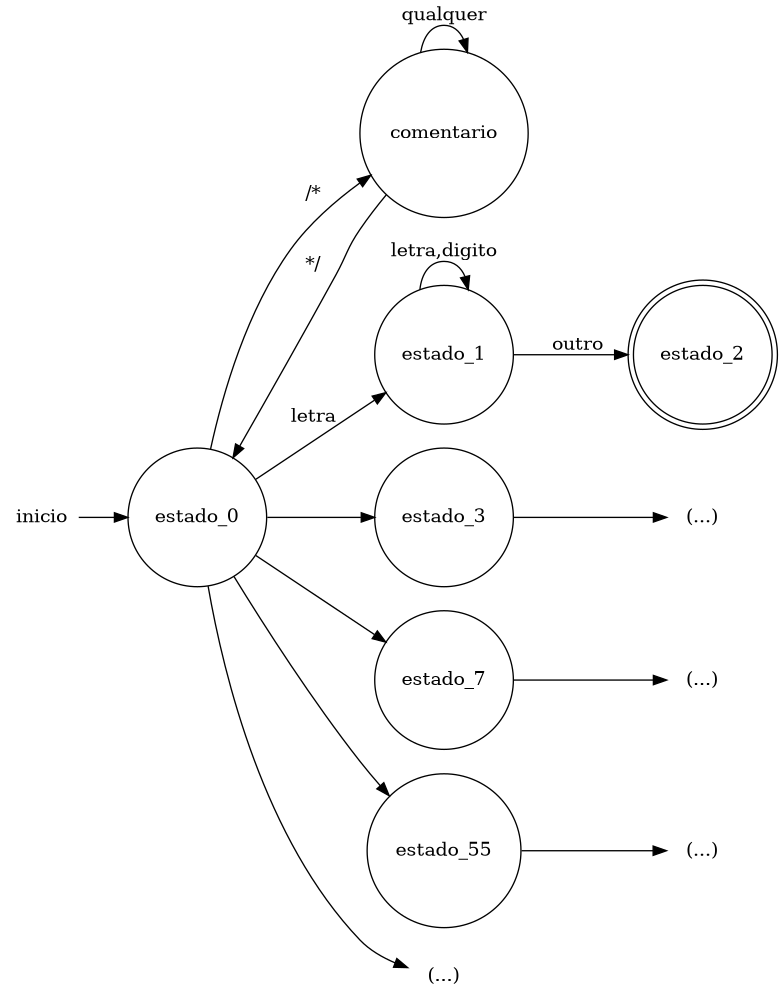
\includegraphics[width=0.7\linewidth,height=\textheight,keepaspectratio]{chapters/images/automato-comentario.png}

}

\caption{\label{fig-af-coment}Comentário para autômatos de estados
finitos}

\end{figure}%

O novo arquivo de especificação Flex que inclui o tratamento para
comentário de linha (//), comentário de múltiplas linhas (/* \ldots{}
*/) e a contagem do número das linhas no arquivo fonte é:

\begin{Shaded}
\begin{Highlighting}[]
\NormalTok{identificador }\OperatorTok{[}\NormalTok{a}\OperatorTok{{-}}\NormalTok{zA}\OperatorTok{{-}}\NormalTok{Z}\OperatorTok{]([}\NormalTok{a}\OperatorTok{{-}}\NormalTok{zA}\OperatorTok{{-}}\NormalTok{Z0}\OperatorTok{{-}}\DecValTok{9}\OperatorTok{])*}
\NormalTok{numero }\OperatorTok{[}\DecValTok{0}\OperatorTok{{-}}\DecValTok{9}\OperatorTok{]+}
\NormalTok{espaco }\OperatorTok{[}\NormalTok{ \textbackslash{}t}\OperatorTok{]+}
\NormalTok{novalinha }\OperatorTok{[}\NormalTok{\textbackslash{}n}\OperatorTok{]}

\OperatorTok{\%}\NormalTok{x coment}

\OperatorTok{\%\{}
    \DataTypeTok{int}\NormalTok{ nlin }\OperatorTok{=} \DecValTok{1}\OperatorTok{;}
\OperatorTok{\%\}}

\OperatorTok{\%\%}
\NormalTok{programa      printf}\OperatorTok{(}\StringTok{"}\SpecialCharTok{\%3d}\StringTok{|}\SpecialCharTok{\%11s}\StringTok{: reservada}\SpecialCharTok{\textbackslash{}n}\StringTok{"}\OperatorTok{,}\NormalTok{ nlin}\OperatorTok{,}\NormalTok{ yytext}\OperatorTok{);}
\NormalTok{inicio        printf}\OperatorTok{(}\StringTok{"}\SpecialCharTok{\%3d}\StringTok{|}\SpecialCharTok{\%11s}\StringTok{: reservada}\SpecialCharTok{\textbackslash{}n}\StringTok{"}\OperatorTok{,}\NormalTok{ nlin}\OperatorTok{,}\NormalTok{ yytext}\OperatorTok{);}
\NormalTok{fimprograma   printf}\OperatorTok{(}\StringTok{"}\SpecialCharTok{\%3d}\StringTok{|}\SpecialCharTok{\%11s}\StringTok{: reservada}\SpecialCharTok{\textbackslash{}n}\StringTok{"}\OperatorTok{,}\NormalTok{ nlin}\OperatorTok{,}\NormalTok{ yytext}\OperatorTok{);}
\NormalTok{leia          printf}\OperatorTok{(}\StringTok{"}\SpecialCharTok{\%3d}\StringTok{|}\SpecialCharTok{\%11s}\StringTok{: reservada}\SpecialCharTok{\textbackslash{}n}\StringTok{"}\OperatorTok{,}\NormalTok{ nlin}\OperatorTok{,}\NormalTok{ yytext}\OperatorTok{);}
\NormalTok{escreva       printf}\OperatorTok{(}\StringTok{"}\SpecialCharTok{\%3d}\StringTok{|}\SpecialCharTok{\%11s}\StringTok{: reservada}\SpecialCharTok{\textbackslash{}n}\StringTok{"}\OperatorTok{,}\NormalTok{ nlin}\OperatorTok{,}\NormalTok{ yytext}\OperatorTok{);}
\NormalTok{se            printf}\OperatorTok{(}\StringTok{"}\SpecialCharTok{\%3d}\StringTok{|}\SpecialCharTok{\%11s}\StringTok{: reservada}\SpecialCharTok{\textbackslash{}n}\StringTok{"}\OperatorTok{,}\NormalTok{ nlin}\OperatorTok{,}\NormalTok{ yytext}\OperatorTok{);}
\NormalTok{entao         printf}\OperatorTok{(}\StringTok{"}\SpecialCharTok{\%3d}\StringTok{|}\SpecialCharTok{\%11s}\StringTok{: reservada}\SpecialCharTok{\textbackslash{}n}\StringTok{"}\OperatorTok{,}\NormalTok{ nlin}\OperatorTok{,}\NormalTok{ yytext}\OperatorTok{);}
\NormalTok{senao         printf}\OperatorTok{(}\StringTok{"}\SpecialCharTok{\%3d}\StringTok{|}\SpecialCharTok{\%11s}\StringTok{: reservada}\SpecialCharTok{\textbackslash{}n}\StringTok{"}\OperatorTok{,}\NormalTok{ nlin}\OperatorTok{,}\NormalTok{ yytext}\OperatorTok{);}
\NormalTok{fimse         printf}\OperatorTok{(}\StringTok{"}\SpecialCharTok{\%3d}\StringTok{|}\SpecialCharTok{\%11s}\StringTok{: reservada}\SpecialCharTok{\textbackslash{}n}\StringTok{"}\OperatorTok{,}\NormalTok{ nlin}\OperatorTok{,}\NormalTok{ yytext}\OperatorTok{);}
\NormalTok{enquanto      printf}\OperatorTok{(}\StringTok{"}\SpecialCharTok{\%3d}\StringTok{|}\SpecialCharTok{\%11s}\StringTok{: reservada}\SpecialCharTok{\textbackslash{}n}\StringTok{"}\OperatorTok{,}\NormalTok{ nlin}\OperatorTok{,}\NormalTok{ yytext}\OperatorTok{);}
\NormalTok{fimenquanto   printf}\OperatorTok{(}\StringTok{"}\SpecialCharTok{\%3d}\StringTok{|}\SpecialCharTok{\%11s}\StringTok{: reservada}\SpecialCharTok{\textbackslash{}n}\StringTok{"}\OperatorTok{,}\NormalTok{ nlin}\OperatorTok{,}\NormalTok{ yytext}\OperatorTok{);}
\NormalTok{inteiro       printf}\OperatorTok{(}\StringTok{"}\SpecialCharTok{\%3d}\StringTok{|}\SpecialCharTok{\%11s}\StringTok{: reservada (tipo)}\SpecialCharTok{\textbackslash{}n}\StringTok{"}\OperatorTok{,}\NormalTok{ nlin}\OperatorTok{,}\NormalTok{ yytext}\OperatorTok{);}
\NormalTok{logico        printf}\OperatorTok{(}\StringTok{"}\SpecialCharTok{\%3d}\StringTok{|}\SpecialCharTok{\%11s}\StringTok{: reservada (tipo)}\SpecialCharTok{\textbackslash{}n}\StringTok{"}\OperatorTok{,}\NormalTok{ nlin}\OperatorTok{,}\NormalTok{ yytext}\OperatorTok{);}

\StringTok{"+"}\NormalTok{          printf}\OperatorTok{(}\StringTok{"}\SpecialCharTok{\%3d}\StringTok{|}\SpecialCharTok{\%11s}\StringTok{: soma}\SpecialCharTok{\textbackslash{}n}\StringTok{"}\OperatorTok{,}\NormalTok{ nlin}\OperatorTok{,}\NormalTok{ yytext}\OperatorTok{);}
\StringTok{"{-}"}\NormalTok{          printf}\OperatorTok{(}\StringTok{"}\SpecialCharTok{\%3d}\StringTok{|}\SpecialCharTok{\%11s}\StringTok{: subtracao}\SpecialCharTok{\textbackslash{}n}\StringTok{"}\OperatorTok{,}\NormalTok{ nlin}\OperatorTok{,}\NormalTok{ yytext}\OperatorTok{);}
\StringTok{"*"}\NormalTok{          printf}\OperatorTok{(}\StringTok{"}\SpecialCharTok{\%3d}\StringTok{|}\SpecialCharTok{\%11s}\StringTok{: multiplicacao}\SpecialCharTok{\textbackslash{}n}\StringTok{"}\OperatorTok{,}\NormalTok{ nlin}\OperatorTok{,}\NormalTok{ yytext}\OperatorTok{);}
\StringTok{"\textless{}{-}"}\NormalTok{         printf}\OperatorTok{(}\StringTok{"}\SpecialCharTok{\%3d}\StringTok{|}\SpecialCharTok{\%11s}\StringTok{: atribuicao}\SpecialCharTok{\textbackslash{}n}\StringTok{"}\OperatorTok{,}\NormalTok{ nlin}\OperatorTok{,}\NormalTok{ yytext}\OperatorTok{);}
\NormalTok{div          printf}\OperatorTok{(}\StringTok{"}\SpecialCharTok{\%3d}\StringTok{|}\SpecialCharTok{\%11s}\StringTok{: divisao}\SpecialCharTok{\textbackslash{}n}\StringTok{"}\OperatorTok{,}\NormalTok{ nlin}\OperatorTok{,}\NormalTok{ yytext}\OperatorTok{);}
\StringTok{"\textgreater{}"}\NormalTok{          printf}\OperatorTok{(}\StringTok{"}\SpecialCharTok{\%3d}\StringTok{|}\SpecialCharTok{\%11s}\StringTok{: maior}\SpecialCharTok{\textbackslash{}n}\StringTok{"}\OperatorTok{,}\NormalTok{ nlin}\OperatorTok{,}\NormalTok{ yytext}\OperatorTok{);}
\StringTok{"\textless{}"}\NormalTok{          printf}\OperatorTok{(}\StringTok{"}\SpecialCharTok{\%3d}\StringTok{|}\SpecialCharTok{\%11s}\StringTok{: menor}\SpecialCharTok{\textbackslash{}n}\StringTok{"}\OperatorTok{,}\NormalTok{ nlin}\OperatorTok{,}\NormalTok{ yytext}\OperatorTok{);}
\StringTok{"="}\NormalTok{          printf}\OperatorTok{(}\StringTok{"}\SpecialCharTok{\%3d}\StringTok{|}\SpecialCharTok{\%11s}\StringTok{: igual}\SpecialCharTok{\textbackslash{}n}\StringTok{"}\OperatorTok{,}\NormalTok{ nlin}\OperatorTok{,}\NormalTok{ yytext}\OperatorTok{);}
\NormalTok{e            printf}\OperatorTok{(}\StringTok{"}\SpecialCharTok{\%3d}\StringTok{|}\SpecialCharTok{\%11s}\StringTok{: e logico}\SpecialCharTok{\textbackslash{}n}\StringTok{"}\OperatorTok{,}\NormalTok{ nlin}\OperatorTok{,}\NormalTok{ yytext}\OperatorTok{);}
\NormalTok{ou           printf}\OperatorTok{(}\StringTok{"}\SpecialCharTok{\%3d}\StringTok{|}\SpecialCharTok{\%11s}\StringTok{: ou logico}\SpecialCharTok{\textbackslash{}n}\StringTok{"}\OperatorTok{,}\NormalTok{ nlin}\OperatorTok{,}\NormalTok{ yytext}\OperatorTok{);}
\NormalTok{nao          printf}\OperatorTok{(}\StringTok{"}\SpecialCharTok{\%3d}\StringTok{|}\SpecialCharTok{\%11s}\StringTok{: negacao}\SpecialCharTok{\textbackslash{}n}\StringTok{"}\OperatorTok{,}\NormalTok{ nlin}\OperatorTok{,}\NormalTok{ yytext}\OperatorTok{);}
\StringTok{"("}\NormalTok{          printf}\OperatorTok{(}\StringTok{"}\SpecialCharTok{\%3d}\StringTok{|}\SpecialCharTok{\%11s}\StringTok{: abre}\SpecialCharTok{\textbackslash{}n}\StringTok{"}\OperatorTok{,}\NormalTok{ nlin}\OperatorTok{,}\NormalTok{ yytext}\OperatorTok{);}
\StringTok{")"}\NormalTok{          printf}\OperatorTok{(}\StringTok{"}\SpecialCharTok{\%3d}\StringTok{|}\SpecialCharTok{\%11s}\StringTok{: fecha}\SpecialCharTok{\textbackslash{}n}\StringTok{"}\OperatorTok{,}\NormalTok{ nlin}\OperatorTok{,}\NormalTok{ yytext}\OperatorTok{);}

\StringTok{"V"}\NormalTok{          printf}\OperatorTok{(}\StringTok{"}\SpecialCharTok{\%3d}\StringTok{|}\SpecialCharTok{\%11s}\StringTok{: constante}\SpecialCharTok{\textbackslash{}n}\StringTok{"}\OperatorTok{,}\NormalTok{ nlin}\OperatorTok{,}\NormalTok{ yytext}\OperatorTok{);}
\StringTok{"F"}\NormalTok{          printf}\OperatorTok{(}\StringTok{"}\SpecialCharTok{\%3d}\StringTok{|}\SpecialCharTok{\%11s}\StringTok{: constante}\SpecialCharTok{\textbackslash{}n}\StringTok{"}\OperatorTok{,}\NormalTok{ nlin}\OperatorTok{,}\NormalTok{ yytext}\OperatorTok{);}

\StringTok{"//"}\OperatorTok{.*}          \OperatorTok{;}
\StringTok{"/*"}\NormalTok{            BEGIN}\OperatorTok{(}\NormalTok{coment}\OperatorTok{);}
\OperatorTok{\textless{}}\NormalTok{coment}\OperatorTok{\textgreater{}}\StringTok{"*/"}\NormalTok{    BEGIN}\OperatorTok{(}\NormalTok{INITIAL}\OperatorTok{);}
\OperatorTok{\textless{}}\NormalTok{coment}\OperatorTok{\textgreater{}.}       \OperatorTok{;} 
\OperatorTok{\textless{}}\NormalTok{coment}\OperatorTok{\textgreater{}}\NormalTok{\textbackslash{}n      nlin}\OperatorTok{++;}

\OperatorTok{\{}\NormalTok{identificador}\OperatorTok{\}}\NormalTok{   printf}\OperatorTok{(}\StringTok{"}\SpecialCharTok{\%3d}\StringTok{|}\SpecialCharTok{\%11s}\StringTok{: identificador}\SpecialCharTok{\textbackslash{}n}\StringTok{"}\OperatorTok{,}\NormalTok{ nlin}\OperatorTok{,}\NormalTok{ yytext}\OperatorTok{);}
\OperatorTok{\{}\NormalTok{numero}\OperatorTok{\}}\NormalTok{          printf}\OperatorTok{(}\StringTok{"}\SpecialCharTok{\%3d}\StringTok{|}\SpecialCharTok{\%11s}\StringTok{: numero}\SpecialCharTok{\textbackslash{}n}\StringTok{"}\OperatorTok{,}\NormalTok{ nlin}\OperatorTok{,}\NormalTok{ yytext}\OperatorTok{);}
\OperatorTok{\{}\NormalTok{espaco}\OperatorTok{\}}          \OperatorTok{;}
\OperatorTok{\{}\NormalTok{novalinha}\OperatorTok{\}}\NormalTok{       nlin}\OperatorTok{++;}

\OperatorTok{\%\%}
\DataTypeTok{int}\NormalTok{ yywrap}\OperatorTok{()} \OperatorTok{\{} \ControlFlowTok{return} \DecValTok{1}\OperatorTok{;} \OperatorTok{\}}
\DataTypeTok{int}\NormalTok{ main }\OperatorTok{()} \OperatorTok{\{}
\NormalTok{    yylex}\OperatorTok{();}
    \ControlFlowTok{return} \DecValTok{0}\OperatorTok{;}
\OperatorTok{\}}
\end{Highlighting}
\end{Shaded}

Para o arquivo Simples de entrada:

\begin{Shaded}
\begin{Highlighting}[]
\NormalTok{/*{-}{-}{-}{-}{-}{-}{-}{-}{-}{-}{-}{-}{-}{-}{-}{-}{-}{-}{-}{-}{-}{-}}
\NormalTok{Programa exemplo em linguagem simples}
\NormalTok{{-}{-}{-}{-}{-}{-}{-}{-}{-}{-}{-}{-}{-}{-}{-}{-}{-}{-}{-}{-}*/}
\KeywordTok{programa}\NormalTok{ um}
  \KeywordTok{inteiro}\NormalTok{ a b  }\CommentTok{// declaracao das variaveis}
\KeywordTok{inicio}
  \KeywordTok{leia}\NormalTok{ a  }\CommentTok{// leitura de a}
  \KeywordTok{leia}\NormalTok{ b  }\CommentTok{// leitura de b}
  \KeywordTok{enquanto}\NormalTok{ a \textless{} b }\KeywordTok{faca}
     \KeywordTok{escreva}\NormalTok{ a }
\NormalTok{     a \textless{}{-} a + }\DecValTok{1}
  \KeywordTok{fimenquanto}
\KeywordTok{fimprograma}
\end{Highlighting}
\end{Shaded}

A saída produzida como resultado do classificador de símbolos
(analisador léxico simplificado) é:

\begin{verbatim}
  4|   programa: reservada
  4|         um: identificador
  5|    inteiro: reservada (tipo)
  5|          a: identificador
  5|          b: identificador
  6|     inicio: reservada
  7|       leia: reservada
  7|          a: identificador
  8|       leia: reservada
  8|          b: identificador
  9|   enquanto: reservada
  9|          a: identificador
  9|          <: menor
  9|          b: identificador
  9|       faca: identificador
 10|    escreva: reservada
 10|          a: identificador
 11|          a: identificador
 11|         <-: atribuicao
 11|          a: identificador
 11|          +: soma
 11|          1: numero
 12|fimenquanto: reservada
 13|fimprograma: reservada
\end{verbatim}

\bookmarksetup{startatroot}

\chapter{As Linguagens Livres de Contexto e a Análise
Sintática}\label{sec-analise-sintatica}

\begin{center}
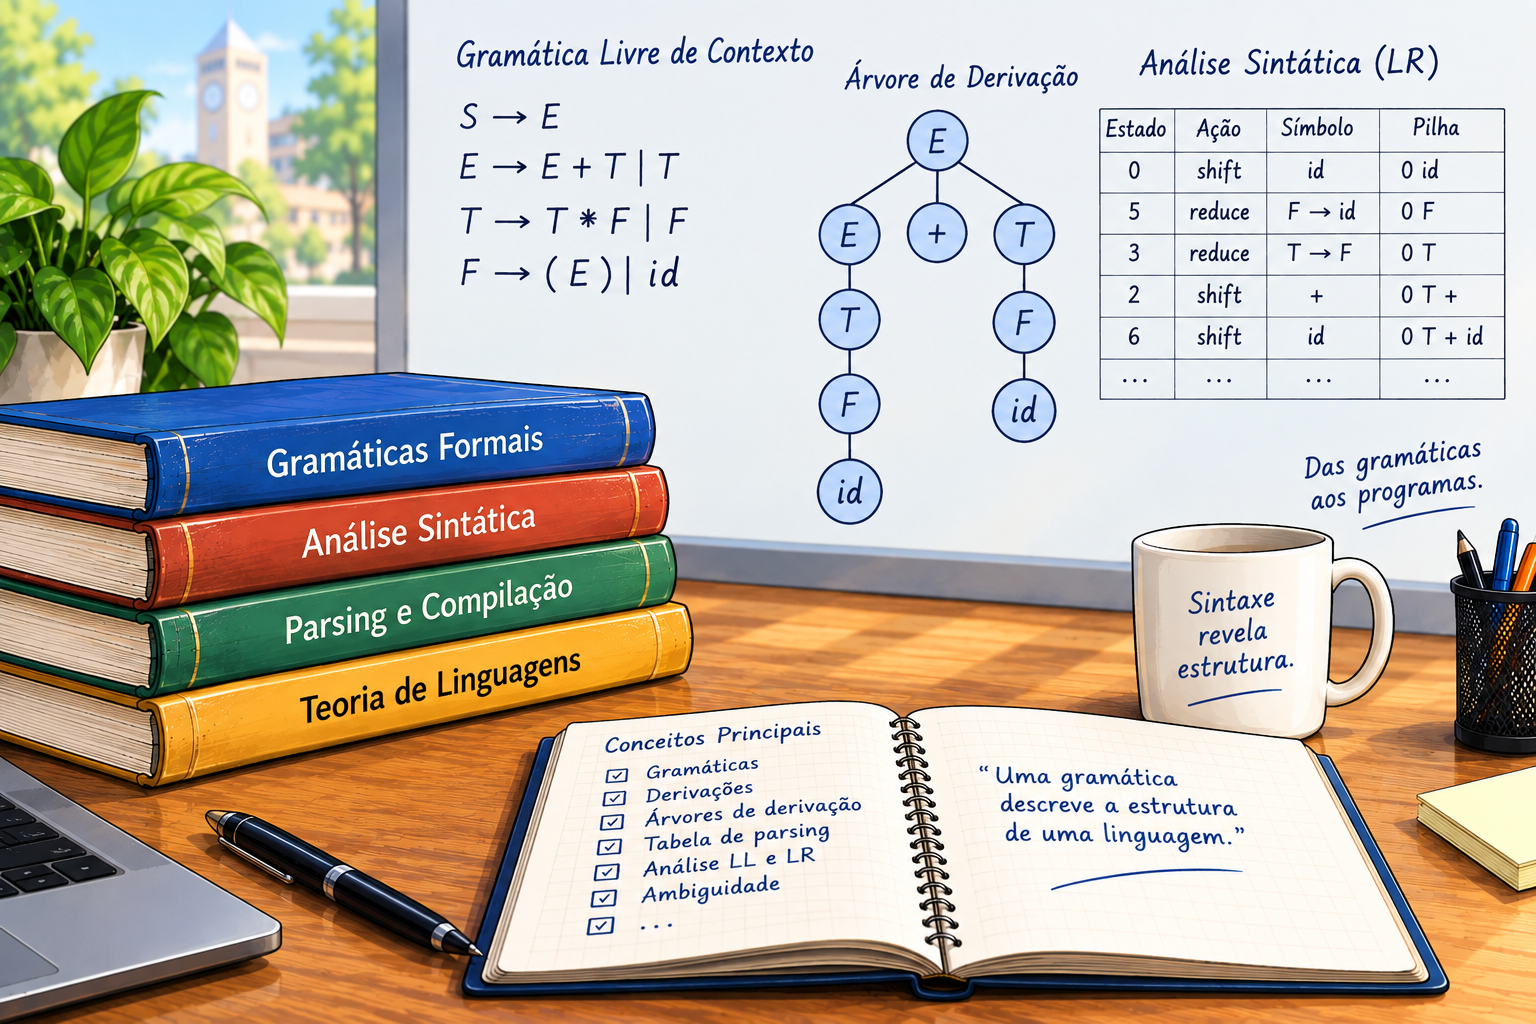
\includegraphics[width=0.7\linewidth,height=\textheight,keepaspectratio]{chapters/images/sintatico.png}
\end{center}

\section{Linguagens Livres de
Contexto}\label{linguagens-livres-de-contexto}

As linguagens regulares constituem uma classe importante de linguagens
formais, mas existem linguagens que não podem ser descritas por meio de
expressões regulares ou reconhecidas por autômatos finitos. Um exemplo
clássico é a linguagem

\[
L = \{0^n1^n \mid n \geq 0\},
\]

que exige que a quantidade de símbolos \texttt{0} seja igual à
quantidade de símbolos \texttt{1}, mantendo ainda a ordem em que esses
símbolos aparecem. Esse tipo de dependência não pode ser mantido por um
autômato finito.

Para descrever linguagens com estruturas desse tipo, utilizam-se as
\textbf{gramáticas livres de contexto (GLC)}. As GLCs constituem um
formalismo mais poderoso que as gramáticas regulares e são
particularmente importantes na especificação da sintaxe das linguagens
de programação. Os analisadores sintáticos dos compiladores utilizam
gramáticas livres de contexto para descrever e verificar as construções
sintáticas de uma linguagem.

As linguagens geradas pelas gramáticas livres de contexto são
denominadas \textbf{linguagens livres de contexto}. No modelo de
reconhecimento, essas linguagens estão associadas aos \textbf{autômatos
de pilha}, uma classe de máquinas que dispõe de uma pilha como memória
auxiliar.

\subsection{Gramáticas Livres de
Contexto}\label{gramuxe1ticas-livres-de-contexto}

Uma gramática consiste em um conjunto de regras, também denominadas
\textbf{produções}, utilizadas para gerar as cadeias pertencentes a uma
linguagem. Cada produção possui uma variável no lado esquerdo e uma
sequência de variáveis e símbolos terminais no lado direito.

Considere, por exemplo, a gramática:

\[
\begin{aligned}
A &\rightarrow aAc\\
A &\rightarrow B\\
B &\rightarrow b
\end{aligned}
\]

Nessa gramática, \(A\) e \(B\) são variáveis, enquanto \(a\), \(b\) e
\(c\) são símbolos terminais. A variável \(A\) é a variável inicial ou
variável de partida.

A produção

\[
A \rightarrow aAc
\]

pode ser utilizada para acrescentar simultaneamente um símbolo
\texttt{a} à esquerda e um símbolo \texttt{c} à direita de uma cadeia. A
produção \(A \rightarrow B\) permite substituir a variável \(A\) por
\(B\), enquanto \$B \rightarrow \texttt{b} encerra o processo de
geração, produzindo o símbolo terminal \texttt{b}.

\subsubsection{Geração de uma cadeia}\label{gerauxe7uxe3o-de-uma-cadeia}

Uma gramática é utilizada para gerar as cadeias de uma linguagem por
meio de sucessivas substituições. Inicialmente, escreve-se a variável
inicial. Em seguida, escolhe-se uma variável presente na forma
sentencial e uma produção que possa ser aplicada a ela. A variável é
então substituída pelo lado direito da produção. Esse processo é
repetido até que não existam mais variáveis na forma sentencial.

Para a gramática apresentada anteriormente, podemos gerar a cadeia
\(aaabccc\) por meio da sequência:

\[
A
\Rightarrow aAc
\Rightarrow aaAcc
\Rightarrow aaaAccc
\Rightarrow aaaBccc
\Rightarrow aaabccc.
\]

A sequência de substituições utilizada para gerar uma cadeia é
denominada \textbf{derivação}. O símbolo \(\Rightarrow\) representa uma
etapa de derivação, enquanto \(\Rightarrow^*\) pode ser utilizado para
representar zero ou mais etapas de derivação.

Nesse exemplo, cada aplicação da produção \(A \rightarrow aAc\)
acrescenta um \texttt{a} no início e um \texttt{c} no final. Depois de
realizadas as substituições necessárias, a variável \(A\) é substituída
por \(B\), e finalmente \(B\) é substituída por \texttt{b}.

\subsubsection{Árvores de
derivação}\label{uxe1rvores-de-derivauxe7uxe3o}

Outra maneira de representar uma derivação é por meio de uma
\textbf{árvore de derivação}. A raiz da árvore corresponde à variável
inicial. Os filhos de um nó correspondem aos símbolos presentes no lado
direito da produção utilizada para expandir a variável representada pelo
nó, conforme ilustrado na Figura~\ref{fig-arvore-derivacao}.

\begin{figure}

\centering{

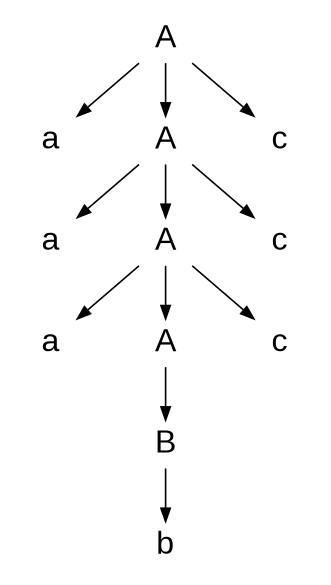
\includegraphics[width=0.3\linewidth,height=\textheight,keepaspectratio]{chapters/images/arvore_derivacao.png}

}

\caption{\label{fig-arvore-derivacao}Árvore de Derivação}

\end{figure}%

Para a derivação de \(aaabccc\), a árvore de derivação representa
graficamente a sequência de aplicações das produções. As folhas da
árvore, lidas da esquerda para a direita, formam a cadeia gerada pela
gramática.

As árvores de derivação são particularmente importantes na análise
sintática de linguagens de programação. Elas permitem representar a
estrutura hierárquica de uma sentença e servem de base para diversas
etapas posteriores do processamento de um programa.

\subsubsection{Definição formal de uma gramática livre de
contexto}\label{definiuxe7uxe3o-formal-de-uma-gramuxe1tica-livre-de-contexto}

\begin{definition}[]\protect\hypertarget{def-glc}{}\label{def-glc}

Uma \textbf{gramática livre de contexto (GLC)} é uma 4-upla

\[
G=(V,\Sigma,R,P),
\]

em que:

\begin{itemize}
\tightlist
\item
  \(V\) é um conjunto finito de \textbf{variáveis};
\item
  \(\Sigma\) é um conjunto finito de \textbf{símbolos terminais},
  disjunto de \(V\);
\item
  \(R\) é um conjunto de regras de produção;
\item
  \(P \in V\) é o símbolo \textbf{inicial} ou de \textbf{partida}.
\end{itemize}

\end{definition}

Cada produção de uma GLC possui a forma

\[
X \rightarrow w,
\]

em que \(X \in V\) e \(w \in (V\cup\Sigma)^*\).

A característica fundamental de uma gramática livre de contexto é que o
lado esquerdo de cada produção contém exatamente uma variável. A
substituição dessa variável pode ser realizada independentemente do
contexto em que ela aparece.

A linguagem gerada por uma gramática \(G\) é definida por

\[
L(G)=\{w\in\Sigma^* \mid P\overset{*}{\Rightarrow}w\}.
\]

Portanto, uma cadeia pertence à linguagem da gramática quando pode ser
derivada a partir do símbolo inicial e, após um número finito de
aplicações das produções, resultar em uma cadeia formada exclusivamente
por símbolos terminais.

\subsubsection{Aplicação das GLCs às linguagens de
programação}\label{aplicauxe7uxe3o-das-glcs-uxe0s-linguagens-de-programauxe7uxe3o}

As gramáticas livres de contexto são amplamente utilizadas para
especificar, por meio de definições indutivas, as construções sintáticas
válidas de linguagens de programação. Em um compilador, a gramática pode
ser utilizada pelo analisador sintático para determinar se a sequência
de tokens produzida pelo analisador léxico possui uma estrutura
sintática válida.

Considere a gramática

\[
G=(\{C,E,I,O\},\{a,b,+,*,(,),:=,;\},R,C),
\]

em que o conjunto de produções é:

\[
\begin{aligned}
C &\rightarrow I:=E \mid C;C\\
E &\rightarrow I \mid EOE \mid (E)\\
O &\rightarrow + \mid *\\
I &\rightarrow a \mid b.
\end{aligned}
\]

A variável \(C\) representa construções de comandos, \(E\) representa
expressões, \(O\) representa operadores e \(I\) representa
identificadores. Essa organização permite descrever estruturas
sintáticas compostas a partir de estruturas menores.

Por exemplo, a produção

\[
E\rightarrow EOE
\]

permite construir uma expressão combinando duas expressões por meio de
um operador. Já a produção

\[
E\rightarrow(E)
\]

permite representar uma expressão delimitada por parênteses.

Essa característica recursiva das GLCs é fundamental para representar
estruturas hierárquicas presentes nas linguagens de programação, como
expressões aritméticas, comandos condicionais, chamadas de funções e
blocos de comandos.

\subsubsection{Outro exemplo de gramática livre de
contexto}\label{outro-exemplo-de-gramuxe1tica-livre-de-contexto}

Considere a gramática

\[
G_3=(\{S\},\{a,b\},R,S),
\]

com as produções

\[
\begin{aligned}
S &\rightarrow aSb\\
S &\rightarrow SS\\
S &\rightarrow \varepsilon.
\end{aligned}
\]

Essa gramática permite gerar cadeias como

\[
abab,\qquad aaabbb,\qquad aababb.
\]

A produção \(S\rightarrow aSb\) permite inserir um símbolo \texttt{a} no
início e um símbolo \texttt{b} no final de uma estrutura. A produção
\(S\rightarrow SS\) permite concatenar duas estruturas já geradas,
enquanto \(S\rightarrow\varepsilon\) fornece o caso básico da derivação.

Se interpretarmos \texttt{a} como um parêntese esquerdo e \texttt{b}
como um parêntese direito, essa gramática está relacionada à linguagem
de parênteses corretamente aninhados. Esse exemplo evidencia a
capacidade das GLCs de representar estruturas recursivas e aninhadas.

\subsubsection{Projeto de gramáticas livres de
contexto}\label{projeto-de-gramuxe1ticas-livres-de-contexto}

A construção de uma GLC para uma determinada linguagem exige a
identificação das estruturas que caracterizam as cadeias dessa
linguagem. Assim como ocorre no projeto de autômatos finitos, não existe
uma única estratégia que possa ser aplicada indistintamente a todos os
problemas.

Uma estratégia útil consiste em decompor uma linguagem em linguagens
livres de contexto mais simples. Considere, por exemplo,

\[
L=\{0^n1^n\mid n\geq0\}
\cup
\{1^n0^n\mid n\geq0\}.
\]

Podemos construir uma gramática para cada uma das partes:

\[
S_1\rightarrow0S_11\mid\varepsilon
\]

e

\[
S_2\rightarrow1S_20\mid\varepsilon.
\]

Em seguida, uma variável inicial pode escolher entre as duas
possibilidades:

\[
S\rightarrow S_1\mid S_2.
\]

Outra estratégia importante é construir uma GLC a partir de um autômato
finito quando a linguagem é regular. Dado um AFD com estados
\(q_0,q_1,\ldots,q_n\), pode-se associar uma variável \(R_i\) a cada
estado \(q_i\).

Para uma transição

\[
\delta(q_i,a)=q_j,
\]

adiciona-se uma produção da forma

\[
R_i\rightarrow aR_j.
\]

Para cada estado de aceitação \(q_i\), adiciona-se também

\[
R_i\rightarrow\varepsilon.
\]

A variável correspondente ao estado inicial do AFD é escolhida como
variável inicial da gramática.

Outra técnica útil para linguagens com dependências entre símbolos
consiste em utilizar produções da forma

\[
R\rightarrow uRv,
\]

nas quais os símbolos acrescentados à esquerda e à direita estão
relacionados. Essa construção é especialmente útil para linguagens que
exigem correspondência entre partes da cadeia, como \(0^n1^n\).

\subsubsection{Ambiguidade}\label{ambiguidade}

Uma GLC é denominada \textbf{ambígua} quando existe pelo menos uma
sentença da linguagem que possui mais de uma árvore de derivação
distinta.

Considere a gramática:

\[
E\rightarrow E+E\mid E*E\mid(E)\mid t.
\]

Para a cadeia

\[
t+t+t,
\]

podem existir diferentes formas de agrupar as operações, conforme
ilustrado na Figura~\ref{fig-ambiguidade}.

\begin{figure}

\centering{

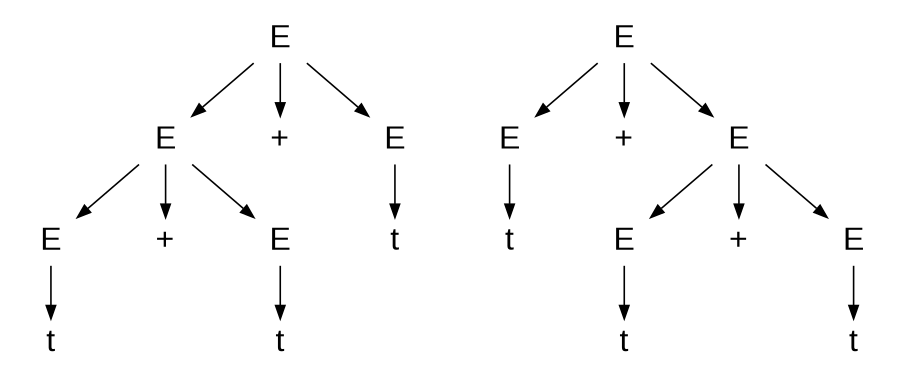
\includegraphics[width=0.7\linewidth,height=\textheight,keepaspectratio]{chapters/images/ambiguidade.png}

}

\caption{\label{fig-ambiguidade}Ambiguidade}

\end{figure}%

Uma interpretação pode associar primeiro os dois primeiros operandos:

\[
(t+t)+t,
\]

enquanto outra pode associar os dois últimos:

\[
t+(t+t).
\]

Essas diferentes estruturas podem ser representadas por árvores de
derivação distintas. A existência de mais de uma árvore para a mesma
sentença caracteriza a ambiguidade da gramática.

A ambiguidade é especialmente importante no projeto de linguagens de
programação, pois uma sentença ambígua pode admitir mais de uma
interpretação sintática. Em uma linguagem de programação, normalmente é
necessário estabelecer regras que determinem de forma única a estrutura
da expressão, como regras de precedência e associatividade dos
operadores.

\subsubsection{Forma Normal de Chomsky}\label{forma-normal-de-chomsky}

Quando se trabalha com gramáticas livres de contexto, pode ser
conveniente transformar a gramática para uma forma simplificada. Uma
dessas formas é a \textbf{Forma Normal de Chomsky (FNC)}.

Uma GLC está na Forma Normal de Chomsky quando suas produções possuem as
formas

\[
A\rightarrow BC
\]

ou

\[
A\rightarrow a,
\]

em que \(A\), \(B\) e \(C\) são variáveis e \(a\) é um símbolo terminal.

Também é permitida a produção

\[
S\rightarrow\varepsilon
\]

quando \(S\) é o símbolo inicial.

A principal característica da FNC é restringir a estrutura das
produções, permitindo que uma variável produza exatamente duas variáveis
ou um único terminal. Essa estrutura simplificada é particularmente
conveniente para determinados algoritmos de análise sintática, entre
eles o algoritmo CYK.

Um resultado importante estabelece que toda gramática livre de contexto
pode ser transformada em uma gramática equivalente na Forma Normal de
Chomsky, considerando as condições apropriadas para a cadeia vazia.

\subsubsection{Transformação para a Forma Normal de
Chomsky}\label{transformauxe7uxe3o-para-a-forma-normal-de-chomsky}

A transformação de uma GLC para a FNC pode ser realizada por uma
sequência de etapas. Inicialmente, introduz-se uma nova variável inicial
\(S_0\) e uma produção

\[
S_0\rightarrow S,
\]

em que \(S\) era o símbolo inicial original. Essa modificação garante
que o novo símbolo inicial não apareça no lado direito de nenhuma
produção.

Em seguida, são removidas as produções \(\varepsilon\). Se uma variável
\(A\) pode produzir \(\varepsilon\), então, para uma produção que
contenha \(A\), devem ser acrescentadas produções correspondentes às
possibilidades de presença ou ausência de \(A\).

Por exemplo, se existir

\[
R\rightarrow uAv
\]

e \(A\) for anulável, pode-se acrescentar

\[
R\rightarrow uv.
\]

Quando uma produção contém várias ocorrências de uma variável anulável,
devem ser consideradas as diferentes combinações possíveis de remoção
dessas ocorrências.

Depois da eliminação das produções \(\varepsilon\), removem-se as
\textbf{produções unitárias}, isto é, produções da forma

\[
A\rightarrow B.
\]

Quando \(B\) possui uma produção \(B\rightarrow u\), a produção
correspondente pode ser transferida para \(A\).

Finalmente, as produções restantes são convertidas para as formas
permitidas pela FNC. Produções com mais de duas variáveis no lado
direito são decompostas por meio da introdução de novas variáveis.

Por exemplo, uma produção

\[
A\rightarrow u_1u_2u_3\ldots u_k
\]

pode ser substituída por uma sequência de produções binárias utilizando
novas variáveis:

\[
\begin{aligned}
A&\rightarrow u_1A_1\\
A_1&\rightarrow u_2A_2\\
&\ \vdots\\
A_{k-2}&\rightarrow u_{k-1}u_k.
\end{aligned}
\]

Quando uma produção de tamanho dois contém terminais, esses terminais
podem ser substituídos por novas variáveis. Por exemplo, para uma
produção contendo \(a\) como um dos símbolos, pode-se introduzir uma
variável \(U\) e a produção

\[
U\rightarrow a.
\]

Dessa maneira, as produções passam gradualmente a obedecer às restrições
da Forma Normal de Chomsky.

\subsubsection{Algoritmo CYK}\label{algoritmo-cyk}

O \textbf{algoritmo de Cocke-Younger-Kasami (CYK)} é um algoritmo de
análise sintática para linguagens livres de contexto. O algoritmo
utiliza uma estratégia de análise de baixo para cima associada à
programação dinâmica.

A versão padrão do CYK opera sobre gramáticas que estão na Forma Normal
de Chomsky. Como toda GLC pode ser transformada para essa forma, o
algoritmo pode ser aplicado, após a transformação apropriada, a uma
ampla classe de linguagens livres de contexto.

Considere uma cadeia de entrada

\[
I=a_1a_2\ldots a_n
\]

e uma gramática em FNC com \(r\) variáveis. O algoritmo mantém
informações sobre quais variáveis podem gerar cada substring da cadeia.

Uma forma de representar essas informações é por meio de uma estrutura
tridimensional

\[
P[n,n,r],
\]

cujos elementos são valores booleanos. Um elemento \(P[l,s,A]\) indica
se a variável \(A\) pode gerar uma substring de comprimento \(l\)
iniciada na posição \(s\) da entrada.

Inicialmente, são identificadas as produções que geram diretamente cada
terminal. Para cada posição \(s\) da entrada e cada produção

\[
R_v\rightarrow a_s,
\]

marca-se:

\[
P[1,s,v]=\text{verdadeiro}.
\]

Em seguida, são analisadas substrings de comprimento crescente. Para uma
substring de comprimento \(l\), consideram-se todas as possíveis
posições iniciais e todas as possíveis divisões da substring em duas
partes.

Suponha que exista uma produção

\[
R_a\rightarrow R_bR_c.
\]

Se uma substring puder ser dividida em duas partes de modo que \(R_b\)
gere a primeira parte e \(R_c\) gere a segunda, então \(R_a\) também
pode gerar a substring completa.

Formalmente, para uma divisão na posição \(p\), verifica-se:

\[
P[p,s,b]\land P[l-p,s+p,c].
\]

Quando essa condição é verdadeira, define-se:

\[
P[l,s,a]=\text{verdadeiro}.
\]

Além da tabela \(P\), pode-se manter uma estrutura de
\textbf{backpointers}, denominada \texttt{back}, contendo informações
sobre as divisões utilizadas para gerar cada substring. Essas
informações permitem reconstruir posteriormente as árvores de derivação
possíveis.

Ao final da execução, verifica-se a posição correspondente à cadeia
completa e à variável inicial. Se

\[
P[n,1,1]
\]

for verdadeiro, a cadeia pertence à linguagem gerada pela gramática.
Caso contrário, a cadeia não pertence à linguagem.

O algoritmo CYK possui complexidade

\[
O(n^3|G|),
\]

em que \(n\) é o tamanho da cadeia de entrada e \(|G|\) representa o
tamanho da gramática. A utilização de programação dinâmica evita a
repetição de cálculos para as mesmas substrings e permite obter um
procedimento sistemático para a análise de cadeias geradas por GLCs em
Forma Normal de Chomsky.

O exemplo interativo seguinte simula esse algoritmo. A partir de um
gramática na Forma Normal de Chomsky e um sentença o simulador preenche
a tabela dinâmica de controi todas as árvores de derivação para a
sentença dada, se esta for reconhecida pela linguagem reconhecida pela
gramática FNC.

\begin{figure}[H]
\centering
\fbox{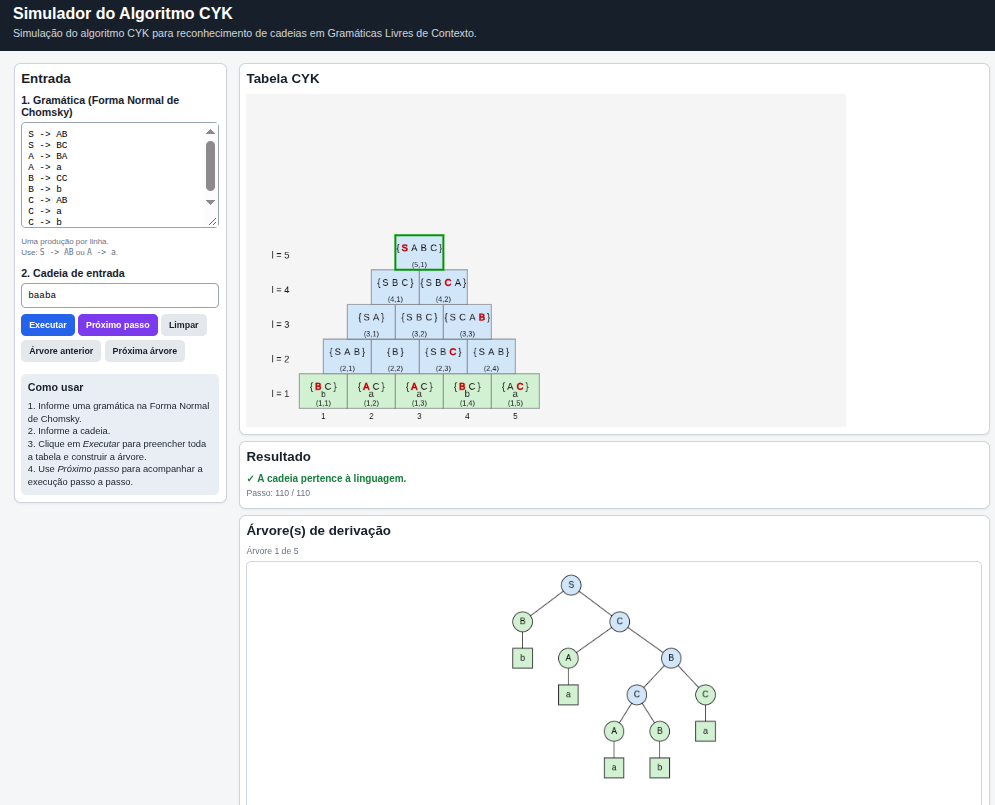
\includegraphics[width=0.6\textwidth]{chapters/images/printscreen/cyk.png}}
\caption{Visualização da aplicação interativa}
\end{figure}
\begin{tcolorbox}[enhanced jigsaw, title=Acesso Interativo]
Acesse a simulação em:\par\smallskip
\small\url{https://luizedsilva.github.io/Livro-LTC/p5js/cyk/}
\begin{center}
\includegraphics[width=3cm]{chapters/images/qrcode/cyk.png}\end{center}
\end{tcolorbox}

\subsubsection{Eliminação da Recursão à
Esquerda}\label{eliminauxe7uxe3o-da-recursuxe3o-uxe0-esquerda}

A recursão à esquerda é uma característica importante das gramáticas
livres de contexto, especialmente quando essas gramáticas são utilizadas
na construção de analisadores sintáticos descendentes. Uma gramática
apresenta recursão à esquerda quando existe uma variável que pode
derivar uma cadeia cujo primeiro símbolo é a própria variável. No caso
mais simples, isso ocorre quando uma produção apresenta a forma

\[
X \rightarrow X\alpha.
\]

A recursão à esquerda pode ser direta, quando aparece explicitamente em
uma produção, ou indireta, quando é introduzida por uma sequência de
derivações envolvendo outras variáveis. Embora a recursão à esquerda não
seja um problema para todos os métodos de análise sintática, ela impede
a aplicação direta de determinados analisadores descendentes, pois o
analisador pode entrar em um processo infinito de expansão de uma mesma
variável sem consumir nenhum símbolo da entrada.

Para uma gramática que contém produções da forma

\[
X \rightarrow Xy_1 \mid Xy_2 \mid \cdots \mid Xy_n
       \mid w_1 \mid w_2 \mid \cdots \mid w_k,
\]

em que os símbolos \(w_i\) não iniciam com \(X\), a recursão à esquerda
pode ser eliminada por meio da introdução de uma nova variável \(Z\). As
produções podem ser substituídas por

\[
X \rightarrow w_1Z \mid w_2Z \mid \cdots \mid w_kZ
\]

e

\[
Z \rightarrow y_1Z \mid y_2Z \mid \cdots \mid y_nZ \mid \lambda.
\]

A transformação preserva a linguagem gerada pela gramática, mas
substitui a recursão à esquerda por uma forma de recursão à direita.

Considere, por exemplo, a gramática

\[
E \rightarrow E+E \mid E*E \mid (E) \mid t.
\]

As duas primeiras produções apresentam recursão à esquerda. Uma
transformação possível, conforme o procedimento apresentado
anteriormente, produz a gramática

\[
E \rightarrow (E)Z \mid tZ
\]

e

\[
Z \rightarrow +EZ \mid *EZ \mid \lambda.
\]

A nova gramática não apresenta a recursão à esquerda direta existente na
gramática original. Essa transformação é particularmente importante para
a construção de analisadores sintáticos descendentes, nos quais a
eliminação da recursão à esquerda constitui uma etapa de preparação da
gramática.

É importante observar que a eliminação da recursão à esquerda não
resolve, por si só, todos os problemas necessários para a construção de
um analisador descendente. Dependendo do método utilizado, outras
transformações podem ser necessárias, como a fatoração à esquerda, além
da análise dos conjuntos FIRST e FOLLOW. Esses conceitos serão
utilizados posteriormente na construção de analisadores LL(1).

\subsection{Autômato com Pilha}\label{autuxf4mato-com-pilha}

As gramáticas livres de contexto podem ser utilizadas para descrever
estruturas que não podem ser reconhecidas por autômatos finitos. Um
exemplo clássico é a linguagem

\[
L=\{0^n1^n\mid n\geq 0\},
\]

na qual a quantidade de símbolos \(0\) deve ser igual à quantidade de
símbolos \(1\). Um autômato finito não possui memória suficiente para
armazenar uma quantidade arbitrária de símbolos e posteriormente
compará-la com a quantidade de símbolos de outro tipo.

Uma estrutura computacional capaz de realizar esse tipo de
reconhecimento é o \textbf{autômato com pilha (AP)}. O autômato com
pilha pode ser entendido como uma extensão de um autômato finito não
determinístico à qual é acrescentada uma estrutura de memória denominada
\textbf{pilha}. Os símbolos podem ser colocados na pilha durante o
processamento da entrada e posteriormente retirados para verificar
relações entre diferentes partes da cadeia.

A pilha funciona segundo o princípio \textbf{LIFO} (\emph{Last In, First
Out}), isto é, o último símbolo inserido é o primeiro a ser retirado.
Essa característica permite que o autômato armazene informações sobre
uma parte da entrada e utilize essas informações posteriormente.

Durante uma transição, o autômato pode ler um símbolo da entrada,
consultar o símbolo que está no topo da pilha e realizar operações sobre
essa pilha. Dependendo da transição, um símbolo pode ser empilhado,
desempilhado ou nenhuma dessas operações pode ser realizada.

Os autômatos com pilha possuem poder computacional equivalente às
gramáticas livres de contexto no que diz respeito às linguagens que
podem ser reconhecidas. Entretanto, existe uma diferença importante
entre autômatos com pilha determinísticos e não determinísticos.
Diferentemente do que ocorre com os autômatos finitos, os autômatos com
pilha determinísticos não possuem o mesmo poder de reconhecimento que os
autômatos com pilha não determinísticos.

\subsubsection{Definição formal de um autômato com
pilha}\label{definiuxe7uxe3o-formal-de-um-autuxf4mato-com-pilha}

\begin{definition}[]\protect\hypertarget{def-ap}{}\label{def-ap}

Um autômato com pilha pode ser definido formalmente pela 6-upla

\[
A=(Q,\Sigma,\Gamma,\delta,q_0,F),
\]

em que:

\begin{itemize}
\tightlist
\item
  \(Q\) é o conjunto finito de estados;
\item
  \(\Sigma\) é o alfabeto de entrada;
\item
  \(\Gamma\) é o alfabeto da pilha;
\item
  \(\delta\) é a função de transição;
\item
  \(q_0\in Q\) é o estado inicial;
\item
  \(F\subseteq Q\) é o conjunto de estados de aceitação.
\end{itemize}

\end{definition}

A função de transição é definida por

\[
\delta:
Q\times\Sigma_\varepsilon\times\Gamma_\varepsilon
\rightarrow
\mathcal{P}(Q\times\Gamma_\varepsilon).
\]

O uso de \(\Sigma_\varepsilon\) permite que uma transição seja realizada
consumindo ou não um símbolo da entrada. Analogamente,
\(\Gamma_\varepsilon\) permite representar situações em que não há
símbolo da pilha sendo consultado ou inserido.

A presença da pilha acrescenta ao modelo de autômato finito uma forma de
memória potencialmente ilimitada. Embora o conjunto de símbolos
disponíveis na pilha seja finito, a quantidade de símbolos armazenados
pode crescer durante a computação. Essa característica é fundamental
para o reconhecimento de diversas linguagens livres de contexto.

\subsubsection{Exemplo de Autômato com
Pilha}\label{exemplo-de-autuxf4mato-com-pilha}

Considere novamente a linguagem

\[
L=\{0^n1^n\mid n\geq0\}.
\]

Um autômato com pilha pode reconhecer essa linguagem armazenando na
pilha um símbolo para cada \(0\) encontrado na entrada. Quando começam a
ser encontrados os símbolos \(1\), o autômato retira um símbolo da pilha
para cada \(1\) lido, representado na Figura~\ref{fig-ap}.

\begin{figure}

\centering{

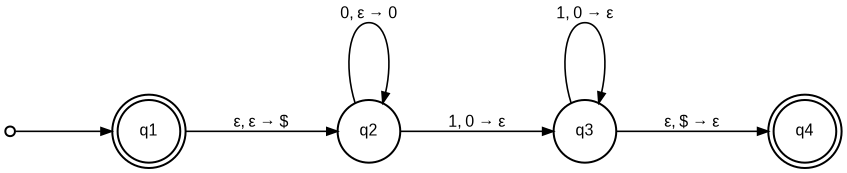
\includegraphics[width=0.8\linewidth,height=\textheight,keepaspectratio]{chapters/images/0n1n.png}

}

\caption{\label{fig-ap}Autômato de Pilha}

\end{figure}%

Inicialmente, a máquina coloca um marcador na pilha para indicar sua
base. Ao processar os símbolos \(0\), um novo símbolo \(0\) é empilhado
para cada símbolo lido. Assim, depois de processar \(0^n\), a pilha
contém \(n\) símbolos \(0\), além do marcador de fundo.

Quando o primeiro \(1\) é encontrado, o autômato passa para uma fase
diferente do processamento. Para cada \(1\) lido, um símbolo \(0\) é
retirado da pilha. Se a cadeia tiver exatamente a mesma quantidade de
\(0\) e \(1\), a leitura da entrada terminará juntamente com o
esvaziamento da parte relevante da pilha.

Essa estratégia permite realizar uma comparação entre duas quantidades
arbitrariamente grandes sem que o autômato precise armazenar
explicitamente o valor de \(n\). A pilha desempenha justamente o papel
dessa memória.

No diagrama de um autômato com pilha, as transições são normalmente
representadas por três componentes. Uma notação possível é

\[
a,b;c,
\]

ou, de forma equivalente,

\[
a,b\rightarrow c.
\]

Essa notação significa que o autômato lê \(a\) da entrada, verifica
\(b\) no topo da pilha e substitui \(b\) por \(c\). Os símbolos podem
ser \(\varepsilon\), permitindo representar diferentes tipos de
transição.

Quando \(a=\varepsilon\), a transição é realizada sem consumir um
símbolo da entrada. Quando \(b=\varepsilon\), não é necessário retirar
um símbolo da pilha para realizar a transição. Finalmente, quando
\(c=\varepsilon\), nenhum símbolo é colocado na pilha após a operação.

Essa notação torna possível representar, em um único diagrama, tanto a
leitura da entrada quanto as operações realizadas sobre a memória
auxiliar do autômato.

O autômato de pilha da Figura~\ref{fig-ap} pode ser formalmente definido
como:

Seja \(M_1 = (Q, \Sigma, \Gamma, \delta, q_1, F)\) e

\[
L(M_1) = \{0^n1^n \mid n \geq 0\}.
\]

Os componentes de \(M_1\) são:

\begin{itemize}
\tightlist
\item
  \(Q = \{q_1, q_2, q_3, q_4\}\);
\item
  \(\Sigma = \{0, 1\}\);
\item
  \(\Gamma = \{0, \$\}\);
\item
  \(F = \{q_1, q_4\}\); e
\item
  \(\delta\) é dada pela tabela a seguir:
\end{itemize}

\small

\begin{longtable*}[]{|
  >{\raggedright\arraybackslash}p{(\linewidth - 20\tabcolsep - 11\arrayrulewidth) * \real{0.0769}}|
  >{\centering\arraybackslash}p{(\linewidth - 20\tabcolsep - 11\arrayrulewidth) * \real{0.1026}}|
  >{\centering\arraybackslash}p{(\linewidth - 20\tabcolsep - 11\arrayrulewidth) * \real{0.1026}}|
  >{\centering\arraybackslash}p{(\linewidth - 20\tabcolsep - 11\arrayrulewidth) * \real{0.1026}}|
  >{\centering\arraybackslash}p{(\linewidth - 20\tabcolsep - 11\arrayrulewidth) * \real{0.1026}}|
  >{\centering\arraybackslash}p{(\linewidth - 20\tabcolsep - 11\arrayrulewidth) * \real{0.1026}}|
  >{\centering\arraybackslash}p{(\linewidth - 20\tabcolsep - 11\arrayrulewidth) * \real{0.1026}}|
  >{\centering\arraybackslash}p{(\linewidth - 20\tabcolsep - 11\arrayrulewidth) * \real{0.1026}}|
  >{\centering\arraybackslash}p{(\linewidth - 20\tabcolsep - 11\arrayrulewidth) * \real{0.1026}}|
  >{\centering\arraybackslash}p{(\linewidth - 20\tabcolsep - 11\arrayrulewidth) * \real{0.1026}}|}
\toprule\noalign{}
\begin{minipage}[b]{\linewidth}\smallskip
\raggedright
Entrada
\end{minipage} & \begin{minipage}[b]{\linewidth}\centering
\end{minipage} & \begin{minipage}[b]{\linewidth}\centering
\textbf{0}
\end{minipage} & \begin{minipage}[b]{\linewidth}\centering
\end{minipage} & \begin{minipage}[b]{\linewidth}\centering
\end{minipage} & \begin{minipage}[b]{\linewidth}\centering
\textbf{1}
\end{minipage} & \begin{minipage}[b]{\linewidth}\centering
\end{minipage} & \begin{minipage}[b]{\linewidth}\centering
\end{minipage} & \begin{minipage}[b]{\linewidth}\centering
\(\varepsilon\)
\end{minipage} & \begin{minipage}[b]{\linewidth}\centering
\end{minipage} \\
\midrule\noalign{}
\endhead
\bottomrule\noalign{}
\endlastfoot
Pilha & \(0\) & \(\$\) & \(\varepsilon\) & \(0\) & \(\$\) &
\(\varepsilon\) & \(0\) & \(\$\) & \(\varepsilon\) \\
\midrule
\(q_1\) & & & & & & & & & \(\{(q_2,\$)\}\) \\
\midrule
\(q_2\) & & & \(\{(q_2,0)\}\) & \(\{(q_3,\varepsilon)\}\) & & & & & \\
\midrule
\(q_3\) & & & & \(\{(q_3,\varepsilon)\}\) & & & &
\(\{(q_4,\varepsilon)\}\) & \\
\midrule
\(q_4\) & & & & & & & & & \\
\end{longtable*}

\normalsize

\subsubsection{Outros exemplos de autômatos com
pilha}\label{outros-exemplos-de-autuxf4matos-com-pilha}

A capacidade adicional fornecida pela pilha permite reconhecer outras
linguagens que não podem ser reconhecidas por autômatos finitos.

Um exemplo apresentado representado na Figura~\ref{fig-ap1}

\[
L(M_2)=
\{a^ib^jc^k\mid i,j,k\geq0
\text{ e } i=j \text{ ou } i=k\}.
\]

\begin{figure}

\centering{

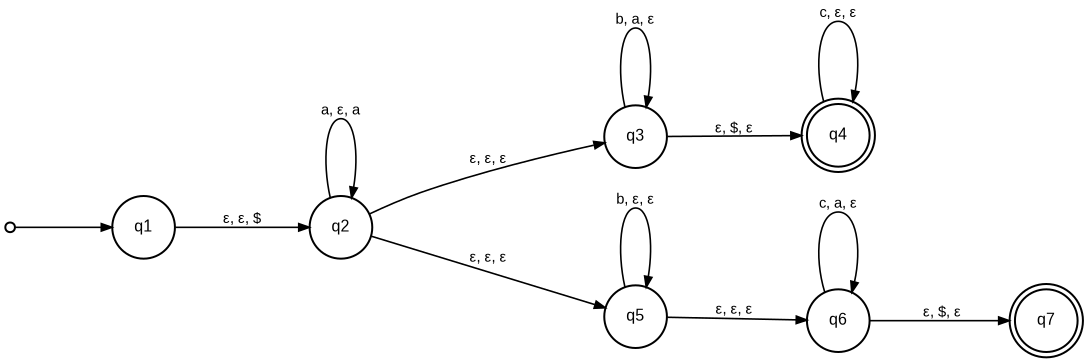
\includegraphics[width=0.8\linewidth,height=\textheight,keepaspectratio]{chapters/images/aibjck.png}

}

\caption{\label{fig-ap1}Autômato de Pilha \(M_2\)}

\end{figure}%

Nesse caso, o autômato precisa verificar uma de duas condições
possíveis: a quantidade de símbolos \(a\) deve ser igual à quantidade de
símbolos \(b\), ou a quantidade de símbolos \(a\) deve ser igual à
quantidade de símbolos \(c\).

O não determinismo é essencial nessa construção. O autômato pode, de
forma não determinística, escolher qual das duas condições tentará
verificar. Essa possibilidade ilustra uma diferença importante entre
autômatos com pilha determinísticos e não determinísticos.

Outro exemplo é a linguagem seguinte, ilustrada na Figura~\ref{fig-ap2}

\[
L(M_3)=\{ww^R\mid w\in\{0,1\}^*\},
\]

\begin{figure}

\centering{

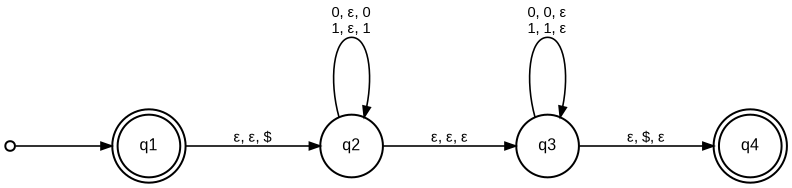
\includegraphics[width=0.8\linewidth,height=\textheight,keepaspectratio]{chapters/images/wwr.png}

}

\caption{\label{fig-ap2}Autômato de Pilha \(M_3\)}

\end{figure}%

formada pelas cadeias obtidas pela concatenação de uma cadeia \(w\) com
sua reversa \(w^R\). O reconhecimento dessa linguagem também exige que o
autômato armazene informações sobre a primeira parte da entrada para
compará-las posteriormente com a segunda parte.

\subsubsection{Equivalência entre Gramáticas Livres de Contexto e
Autômatos com
Pilha}\label{equivaluxeancia-entre-gramuxe1ticas-livres-de-contexto-e-autuxf4matos-com-pilha}

Existe uma relação fundamental entre gramáticas livres de contexto e
autômatos com pilha. O resultado pode ser expresso pelo seguinte
teorema:

\begin{theorem}[]\protect\hypertarget{thm-eq-glc-ap}{}\label{thm-eq-glc-ap}

Uma linguagem é livre de contexto se, e somente se, algum autômato com
pilha a reconhece.

\end{theorem}

Esse resultado estabelece uma equivalência entre duas formas diferentes
de representar uma mesma classe de linguagens. Uma linguagem livre de
contexto pode ser descrita por meio de uma \textbf{gramática}, que
especifica como suas cadeias podem ser geradas, ou por meio de um
\textbf{autômato com pilha}, que especifica como suas cadeias podem ser
reconhecidas.

A equivalência não significa que uma gramática e um autômato com pilha
tenham a mesma estrutura. Na gramática, o processo é descrito por meio
de produções e derivações. No autômato, o processamento é descrito por
estados, transições e operações sobre a pilha.

Podemos, portanto, considerar duas direções de transformação:

\[
\text{GLC}\longrightarrow\text{AP}
\]

e

\[
\text{AP}\longrightarrow\text{GLC}.
\]

Essas transformações mostram que os dois formalismos possuem exatamente
o mesmo poder de representação para a classe das linguagens livres de
contexto.

\subsubsection{Construção de um autômato com pilha a partir de uma
GLC}\label{construuxe7uxe3o-de-um-autuxf4mato-com-pilha-a-partir-de-uma-glc}

Considere a gramática

\[
\begin{aligned}
S &\rightarrow aXb\mid c,\\
X &\rightarrow aX\mid\varepsilon.
\end{aligned}
\]

A construção de um autômato com pilha a partir de uma GLC pode ser feita
de forma que a pilha contenha uma representação da derivação que ainda
precisa ser processada.

\begin{figure}

\centering{

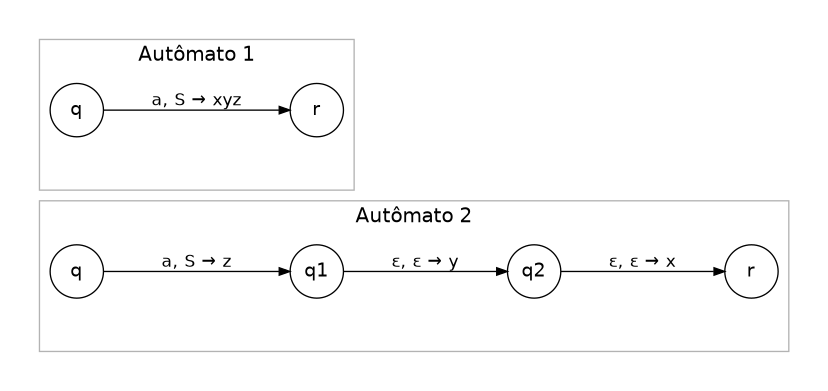
\includegraphics[width=0.8\linewidth,height=\textheight,keepaspectratio]{chapters/images/modelo-glc-ap.png}

}

\caption{\label{fig-modelo-glc-ap}Modelo de conversão GLC para AP}

\end{figure}%

Inicialmente, o símbolo inicial da gramática é colocado na pilha. O
autômato utiliza as produções da gramática para substituir uma variável
pelo lado direito de uma produção. Esse processo pode ser realizado por
transições que não consomem símbolos da entrada, conforme ilustrado na
transformacão do autômato 1 para o autômato 2 na
Figura~\ref{fig-modelo-glc-ap}.

Quando o topo da pilha é um terminal, o autômato compara esse terminal
com o próximo símbolo da entrada. Se forem iguais, o símbolo é consumido
e retirado da pilha. Dessa maneira, a pilha mantém uma representação da
parte da derivação que ainda precisa ser reconhecida.

O procedimento estabelece uma correspondência entre uma derivação da
gramática e uma computação do autômato. A aceitação ocorre quando toda a
entrada foi consumida e a representação da derivação foi processada.

A conversão da gramática livre de contexto para o autômatro de pilha
correspondente está representado na Figura~\ref{fig-glc-ap}.

\begin{figure}

\centering{

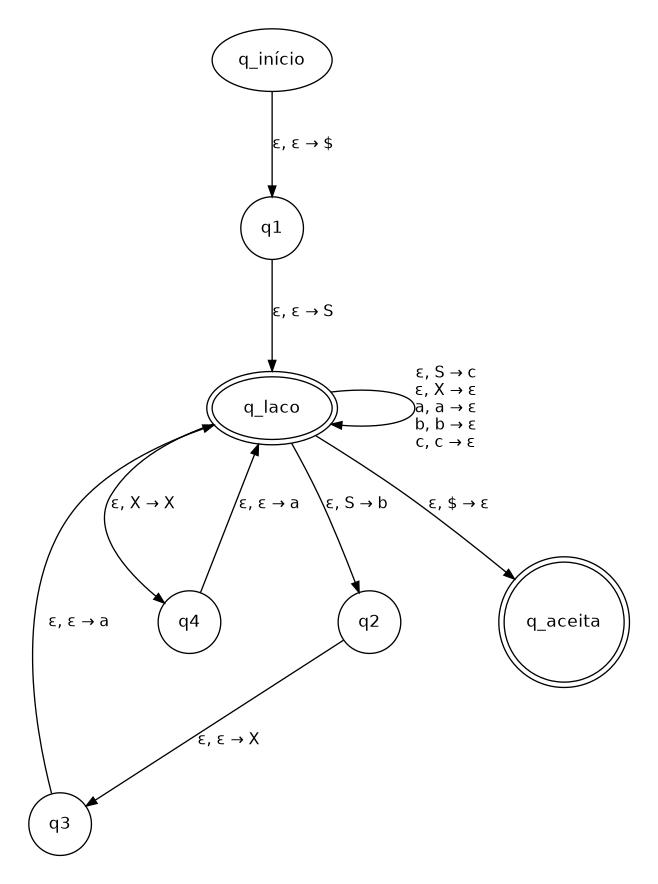
\includegraphics[width=0.8\linewidth,height=\textheight,keepaspectratio]{chapters/images/glc-ap.png}

}

\caption{\label{fig-glc-ap}Conversão GLC para AP}

\end{figure}%

No nó laço estão representadas todas as regras da gramática:

\begin{itemize}
\tightlist
\item
  No laço de q\_laço para q\_laço estão o empilhamento dos terminais,
  por exemplo, \(a, a \rightarrow \varepsilon\) que significa que quando
  o autômato de pilha lê o símbolo \(a\) ele empilha o símbolo \(a\) e
  não desempilha nada (\(\varepsilon\)). Nesta transição estão as regras
  unitária também, como \(S \rightarrow c\), representado como operação
  de pilha \(\varepsilon, S \rightarrow c\).
\item
  Nas transições q\_laço \(\rightarrow\) q4 \(\rightarrow\) q\_laço,
  estão as operações de pilha correspondentes a regra
  \(X \rightarrow aX\).
\item
  E nas transições q\_laço \(\rightarrow\) q2 \(\rightarrow\) q3
  \(\rightarrow\) q\_laço, estão as operações de pilha correspondentes a
  regra \(S \rightarrow aXb\).
\end{itemize}

\subsubsection{Construção de uma GLC a partir de um autômato com
pilha}\label{construuxe7uxe3o-de-uma-glc-a-partir-de-um-autuxf4mato-com-pilha}

A transformação inversa também é possível. Considere um autômato com
pilha

\[
P=(Q,\Sigma,\Gamma,\delta,q_0,\{q_{\mathrm{aceita}}\}).
\]

Pode-se construir uma gramática

\[
G=(V,\Sigma,R,P)
\]

na qual as variáveis representam computações do autômato entre pares de
estados.

Para cada par de estados \(p,q\in Q\), é criada uma variável

\[
A_{pq}.
\]

Intuitivamente, \(A_{pq}\) representa uma cadeia de entrada que permite
ao autômato sair do estado \(p\) e chegar ao estado \(q\), obedecendo às
operações necessárias sobre a pilha.

O símbolo inicial da gramática é definido por

\[
A_{q_0,q_{\mathrm{aceita}}}.
\]

As regras de produção são construídas a partir das transições do
autômato. Entre elas encontram-se regras da forma

\[
A_{pq}\rightarrow aA_{rs}b,
\]

regras que dividem uma computação em duas partes,

\[
A_{pq}\rightarrow A_{pr}A_{rq},
\]

e regras que representam uma computação que começa e termina no mesmo
estado,

\[
A_{pp}\rightarrow\varepsilon.
\]

Essa construção é mais complexa do que a transformação de uma GLC para
um autômato com pilha, mas demonstra formalmente a equivalência entre os
dois modelos.

\subsection{Linguagens que não são Livres de
Contexto}\label{linguagens-que-nuxe3o-suxe3o-livres-de-contexto}

As gramáticas livres de contexto são bastante expressivas, mas não
conseguem representar todas as linguagens formais. Portanto, assim como
foi possível identificar linguagens que não são regulares, também é
possível identificar linguagens que não são livres de contexto.

Um exemplo clássico é

\[
L=\{a^ib^ic^i\mid i>0\}.
\]

Para pertencer a essa linguagem, uma cadeia deve possuir a mesma
quantidade de símbolos \(a\), \(b\) e \(c\), nessa ordem. Uma única
pilha não é suficiente para realizar esse tipo de comparação simultânea
entre três quantidades independentes.

Para demonstrar formalmente que uma linguagem não é livre de contexto,
uma das ferramentas utilizadas é o \textbf{lema do bombeamento para
linguagens livres de contexto}.

\subsection{Lema do Bombeamento para Linguagens Livres de
Contexto}\label{lema-do-bombeamento-para-linguagens-livres-de-contexto}

O lema do bombeamento fornece uma propriedade que toda linguagem livre
de contexto deve satisfazer. Se \(A\) é uma linguagem livre de contexto,
então existe um número inteiro \(p\), chamado \textbf{comprimento de
bombeamento}, tal que toda cadeia \(s\in A\), com comprimento
suficientemente grande, pode ser dividida em cinco partes:

\[
s=uvxyz,
\]

de modo que sejam satisfeitas as seguintes condições:

\[
|vy|>0,
\]

\[
|vxy|\leq p,
\]

e, para todo \(i\geq0\),

\[
uv^ixy^iz\in A.
\]

A primeira condição garante que pelo menos uma das partes \(v\) ou \(y\)
seja não vazia. A segunda estabelece que as partes \(v\), \(x\) e \(y\)
estão contidas em uma região da cadeia cujo comprimento não ultrapassa
\(p\). A terceira é a propriedade de bombeamento propriamente dita: as
partes \(v\) e \(y\) podem ser repetidas simultaneamente qualquer número
de vezes sem que a cadeia deixe de pertencer à linguagem.

O lema é normalmente utilizado para provar que uma linguagem \textbf{não
é} livre de contexto. Para isso, supõe-se inicialmente que a linguagem
seja livre de contexto. A partir dessa hipótese, utiliza-se o
comprimento de bombeamento garantido pelo lema e escolhe-se
cuidadosamente uma cadeia pertencente à linguagem. Em seguida,
demonstra-se que qualquer decomposição possível da cadeia viola uma das
propriedades exigidas pelo lema.

É importante observar que o lema do bombeamento fornece uma
\textbf{condição necessária}, mas não suficiente, para uma linguagem ser
livre de contexto. Portanto, se uma linguagem não satisfaz o lema,
podemos concluir que ela não é livre de contexto. Por outro lado,
satisfazer o lema não constitui, isoladamente, uma prova de que a
linguagem seja livre de contexto.

\subsubsection{Exemplo de Linguagem que não é Livre de
Contexto}\label{exemplo-de-linguagem-que-nuxe3o-uxe9-livre-de-contexto}

Considere novamente

\[
L=\{a^ib^ic^i\mid i>0\}.
\]

Suponha, por contradição, que \(L\) seja uma linguagem livre de
contexto. Pelo lema do bombeamento, existe um comprimento de bombeamento
\(p\). Escolhemos então a cadeia

\[
s=a^pb^pc^p.
\]

Claramente,

\[
s\in L.
\]

Pelo lema, essa cadeia pode ser dividida como

\[
s=uvxyz,
\]

satisfazendo

\[
|vxy|\leq p.
\]

A escolha da cadeia é importante porque existem três blocos
consecutivos, cada um com comprimento \(p\):

\[
\underbrace{aa\cdots a}_{p}
\underbrace{bb\cdots b}_{p}
\underbrace{cc\cdots c}_{p}.
\]

Como \(vxy\) possui comprimento no máximo \(p\), essa região não pode
abranger simultaneamente partes dos três blocos. Portanto, \(vxy\) está
contido em um único bloco ou atravessa apenas uma das fronteiras entre
dois blocos.

Consequentemente, existem casos em que \(vxy\) possui apenas símbolos
\(a\), apenas símbolos \(b\) ou apenas símbolos \(c\), e casos em que
possui símbolos \(a\) e \(b\), ou símbolos \(b\) e \(c\). Não é possível
que contenha simultaneamente os três tipos de símbolos.

As possibilidades relevantes são, portanto,

\[
vxy=a^j,
\]

\[
vxy=a^jb^k,
\]

\[
vxy=b^j,
\]

\[
vxy=b^jc^k,
\]

ou

\[
vxy=c^j.
\]

Ao bombear, por exemplo, com \(i=2\), obtemos

\[
uv^2xy^2z.
\]

Nessa nova cadeia, a quantidade de símbolos modificada em pelo menos um
dos blocos não é acompanhada por uma modificação equivalente nos demais
blocos. Consequentemente, a cadeia resultante deixa de possuir a forma

\[
a^ib^ic^i.
\]

Isso contradiz a primeira condição do lema do bombeamento, segundo a
qual a cadeia bombeada deveria continuar pertencendo à linguagem para
todo \(i\geq0\).

Portanto, a hipótese inicial é falsa e concluímos que

\[
\boxed{\{a^ib^ic^i\mid i>0\}\text{ não é uma linguagem livre de contexto}.}
\]

Esse exemplo evidencia uma limitação fundamental das linguagens livres
de contexto: embora sejam capazes de representar relações de dependência
importantes, como o balanceamento de parênteses ou a correspondência
entre duas quantidades, existem relações entre três ou mais componentes
que não podem ser reconhecidas por um único mecanismo de pilha.

\section{Análise Sintática}\label{anuxe1lise-sintuxe1tica-1}

A \textbf{análise sintática} constitui uma das principais etapas da fase
de análise de um compilador. Ela é realizada pelo \textbf{analisador
sintático}, também denominado \emph{parser}, que recebe como entrada a
sequência de \emph{tokens} produzida pelo analisador léxico e verifica
se essa sequência está de acordo com as regras sintáticas da linguagem
de programação.

Enquanto o analisador léxico identifica os elementos básicos do
programa, como identificadores, palavras reservadas, operadores, números
e delimitadores, o analisador sintático trabalha com esses elementos
para determinar como eles estão relacionados entre si. Seu objetivo é
reconhecer estruturas maiores, como expressões, comandos, declarações,
blocos e programas completos.

Por exemplo, considere uma expressão como:

\[
a+b*c.
\]

O analisador léxico pode produzir uma sequência de \emph{tokens}
correspondente a:

\[
\text{IDENT}(a),\quad +,\quad \text{IDENT}(b),\quad *,\quad \text{IDENT}(c).
\]

A análise sintática deve determinar como esses \emph{tokens} podem ser
agrupados de acordo com a gramática da linguagem. Nesse caso, uma
gramática que estabeleça a precedência da multiplicação sobre a adição
poderá determinar que a expressão seja estruturada como

\[
a+(b*c).
\]

Dessa forma, a análise sintática não se limita a verificar se os
\emph{tokens} aparecem em uma determinada ordem. Ela também determina a
\textbf{estrutura hierárquica} da sentença.

\subsection{Estrutura sintática}\label{estrutura-sintuxe1tica}

Uma das principais estruturas utilizadas para representar o resultado da
análise sintática é a \textbf{árvore sintática}. A árvore representa a
aplicação das regras sintáticas da linguagem e organiza hierarquicamente
os elementos que compõem o programa.

De maneira geral, os nós internos da árvore representam construções
sintáticas da linguagem, enquanto as folhas correspondem aos símbolos
terminais ou aos \emph{tokens} que constituem a sentença de entrada. A
raiz representa a estrutura mais abrangente reconhecida pela gramática,
normalmente associada ao símbolo inicial.

Considere, por exemplo, uma expressão aritmética. Uma possível árvore
sintática para

\[
a+b*c
\]

pode representar a estrutura:

\begin{figure}[H]

{\centering 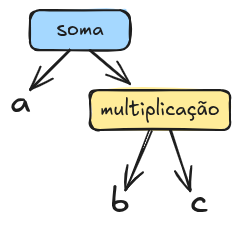
\includegraphics[width=0.4\linewidth,height=\textheight,keepaspectratio]{chapters/images/expressao.png}

}

\caption{extrutura sintática da expressão}

\end{figure}%

A árvore evidencia que a multiplicação de \(b\) por \(c\) constitui uma
subestrutura da expressão e que seu resultado é utilizado como segundo
operando da adição.

Essa representação é particularmente importante porque a estrutura
sintática pode ser utilizada pelas etapas seguintes do compilador. A
partir dela, por exemplo, podem ser realizadas análises semânticas,
verificações de tipos e transformações necessárias para a geração de
código.

\subsection{Gramática e reconhecimento
sintático}\label{gramuxe1tica-e-reconhecimento-sintuxe1tico}

A estrutura sintática de uma linguagem é normalmente especificada por
meio de uma \textbf{gramática livre de contexto (GLC)}. A gramática
define as construções que podem ser formadas e as relações existentes
entre elas.

Considere uma gramática simplificada para expressões:

\[
\begin{aligned}
E &\rightarrow E+T \mid T\\
T &\rightarrow T*F \mid F\\
F &\rightarrow (E) \mid id.
\end{aligned}
\]

Nessa gramática, \(E\) representa uma expressão, \(T\) representa um
termo e \(F\) representa um fator. As produções estabelecem, entre
outras propriedades, a precedência dos operadores \texttt{+} e
\texttt{*}.

O analisador sintático utiliza as produções da gramática para verificar
se a sequência de \emph{tokens} recebida pode ser derivada a partir do
símbolo inicial. Se for possível realizar uma derivação que produza
exatamente a sequência de entrada, a sentença é considerada
sintaticamente válida.

Assim, para uma cadeia de entrada \(w\), o problema fundamental da
análise sintática pode ser expresso como a determinação de

\[
S\Rightarrow^* w,
\]

em que \(S\) é o símbolo inicial da gramática.

Quando a cadeia não pode ser derivada a partir do símbolo inicial, o
analisador sintático identifica uma \textbf{erro sintático}. Nesse caso,
o compilador normalmente informa a ocorrência do erro e sua localização
aproximada no programa-fonte.

\subsection{Árvore de derivação e árvore
sintática}\label{uxe1rvore-de-derivauxe7uxe3o-e-uxe1rvore-sintuxe1tica}

É importante distinguir a \textbf{árvore de derivação} da \textbf{árvore
sintática}. A árvore de derivação representa explicitamente a aplicação
das produções da gramática. Ela contém, portanto, os elementos
intermediários utilizados durante a derivação da sentença.

A árvore sintática, por sua vez, normalmente é uma representação mais
compacta da estrutura reconhecida. Elementos que são relevantes para a
derivação, mas que não são necessários para representar a estrutura
sintática da construção, podem ser eliminados.

Por exemplo, uma árvore de derivação pode conter variáveis como \(E\),
\(T\) e \(F\) em diversos níveis, enquanto uma árvore sintática pode
representar diretamente a relação entre operadores e operandos.

Essa distinção é importante no desenvolvimento de compiladores porque
diferentes analisadores sintáticos podem produzir estruturas
intermediárias distintas, mas que representam a mesma estrutura
sintática essencial do programa.

\subsection{Correção sintática}\label{correuxe7uxe3o-sintuxe1tica}

Um programa está \textbf{sintaticamente correto} quando sua sequência de
\emph{tokens} pode ser reconhecida pela gramática da linguagem. Em
termos formais, isso significa que existe uma derivação a partir do
símbolo inicial da gramática que produz exatamente a sequência de
entrada.

Quando se considera uma gramática não ambígua, espera-se que uma
sentença válida possua uma única estrutura sintática. Nesse caso, a
árvore sintática representa de maneira não ambígua a organização dos
elementos da sentença.

A existência de mais de uma árvore de derivação para uma mesma sentença
caracteriza uma \textbf{gramática ambígua}. A ambiguidade pode ser
problemática em linguagens de programação porque diferentes árvores
podem representar diferentes interpretações para uma mesma sequência de
\emph{tokens}. Por esse motivo, as gramáticas utilizadas na
especificação de linguagens de programação devem ser projetadas de forma
a evitar ambiguidades ou devem ser acompanhadas de regras que permitam
determinar univocamente a estrutura pretendida.

\subsection{Analisador sintático}\label{analisador-sintuxe1tico}

O analisador sintático recebe a sequência de \emph{tokens} produzida
pelo analisador léxico e procura determinar se ela pertence à linguagem
definida pela gramática.

De forma simplificada, seu funcionamento pode ser representado por:

\begin{figure}

\centering{

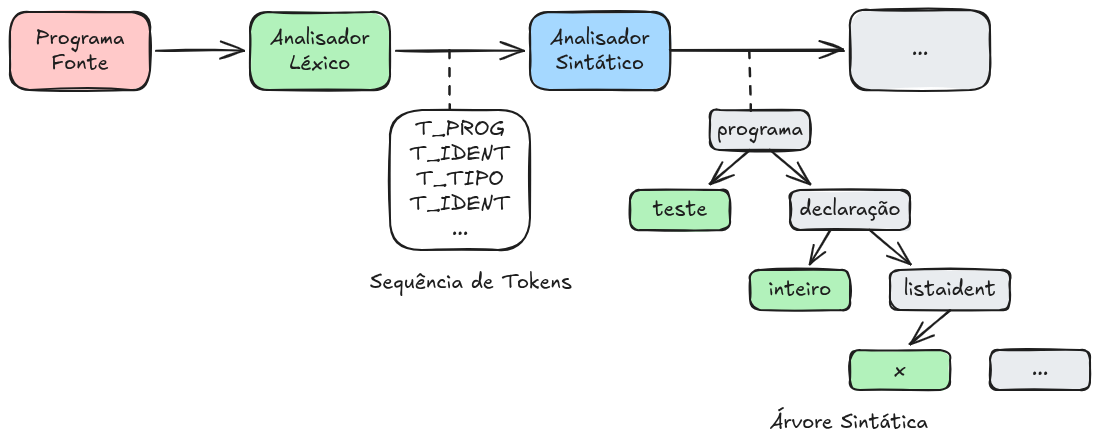
\includegraphics[width=0.8\linewidth,height=\textheight,keepaspectratio]{chapters/images/lexico-sintatico.png}

}

\caption{\label{fig-lexico-sintatico}Processo de integração dos
analisadores léxico e sintático}

\end{figure}%

Durante esse processo, o analisador sintático pode construir diretamente
uma árvore ou utilizar estruturas auxiliares para posteriormente
produzir a árvore correspondente. Em outros casos, a implementação pode
produzir uma representação intermediária que será utilizada pelas etapas
posteriores do compilador.

Quando a entrada não está de acordo com a gramática, o analisador deve
detectar o erro sintático. Além de identificar que a sentença não
pertence à linguagem, um analisador sintático de um compilador deve,
sempre que possível, fornecer informações úteis para a localização e
recuperação do erro.

\subsection{Análise sintática descendente e
ascendente}\label{anuxe1lise-sintuxe1tica-descendente-e-ascendente}

Existem diferentes estratégias para implementar um analisador sintático.
Duas famílias importantes são a \textbf{análise sintática descendente} e
a \textbf{análise sintática ascendente}.

Na análise descendente (\emph{top-down}), a construção da estrutura
sintática parte do símbolo inicial da gramática e procura produzir a
sequência de \emph{tokens} da entrada. O processo pode ser interpretado
como uma construção da árvore a partir da raiz em direção às folhas.

Uma das técnicas mais conhecidas dessa família é a análise \textbf{LL},
na qual a entrada é examinada da esquerda para a direita e a derivação
utilizada é uma derivação mais à esquerda.

Na análise ascendente (\emph{bottom-up}), o processo ocorre na direção
inversa. O analisador parte dos \emph{tokens} da entrada e procura
agrupá-los em estruturas maiores até chegar ao símbolo inicial da
gramática. Esse processo pode ser interpretado como uma construção da
árvore sintática das folhas em direção à raiz.

Os métodos \textbf{LR} constituem uma importante família de analisadores
sintáticos ascendentes. Nesses métodos, a análise é realizada por meio
de operações como deslocamento (\emph{shift}) e redução (\emph{reduce}).

As técnicas LL e LR serão estudadas posteriormente neste capítulo. Antes
disso, é necessário revisar os conceitos fundamentais utilizados na
especificação e análise de linguagens, incluindo gramáticas, gramáticas
livres de contexto, derivações, reduções, árvores de derivação e árvores
sintáticas.

\subsection{Relação com as demais etapas do
compilador}\label{relauxe7uxe3o-com-as-demais-etapas-do-compilador}

A análise sintática estabelece uma ligação entre a sequência linear de
\emph{tokens} produzida pelo analisador léxico e a estrutura hierárquica
necessária para as etapas posteriores do compilador.

O fluxo simplificado pode ser representado da seguinte forma:

\begin{figure}[H]

{\centering 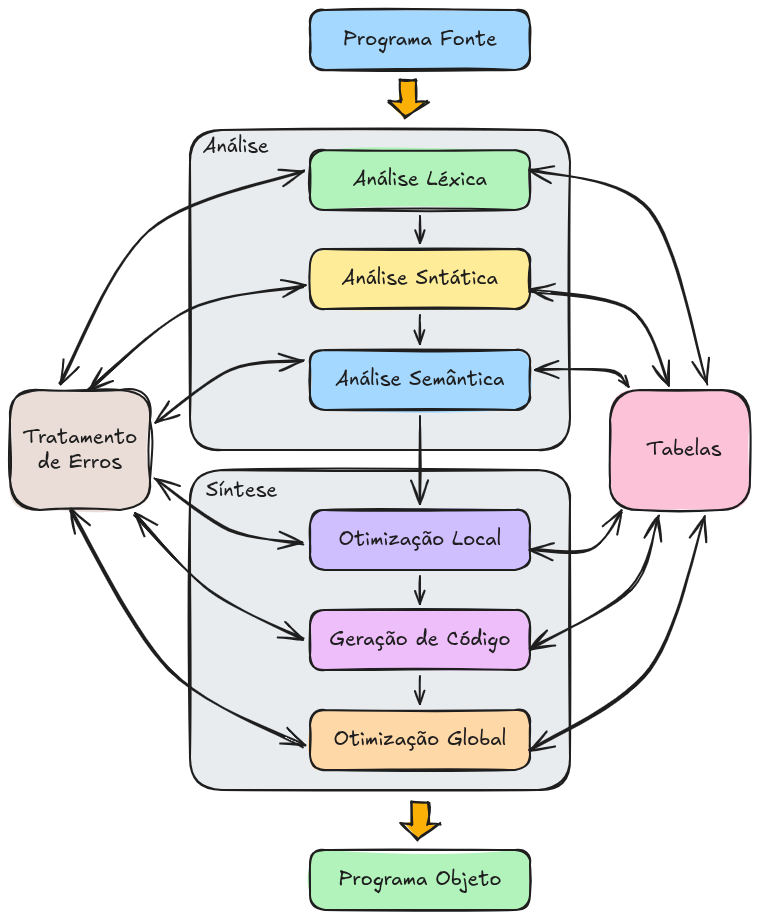
\includegraphics[width=0.6\linewidth,height=\textheight,keepaspectratio]{chapters/images/fases.png}

}

\caption{Fases do compilador}

\end{figure}%

A análise léxica identifica os elementos básicos do programa, enquanto a
análise sintática determina como esses elementos estão organizados. A
partir da estrutura sintática reconhecida, a análise semântica pode
verificar propriedades que não são determinadas exclusivamente pela
gramática, como compatibilidade de tipos, declaração e uso de
identificadores e outras restrições semânticas da linguagem.

Dessa forma, a análise sintática desempenha um papel fundamental na
organização do programa para as etapas seguintes da compilação. Uma
sequência de \emph{tokens} deixa de ser apenas uma lista linear de
elementos e passa a ser interpretada como uma estrutura hierárquica de
acordo com as regras definidas pela linguagem.

Em seguida, serão estudadas as principais estratégias de implementação
de analisadores sintáticos, com destaque para os métodos \textbf{LL} e
\textbf{LR}.

\section{Implementação de Analisadores
Sintáticos}\label{implementauxe7uxe3o-de-analisadores-sintuxe1ticos}

O objetivo principal da análise sintática é decidir se uma cadeia
(sentença, palavra) pertence ou não à linguagem definida por uma
gramática. Existem duas importantes estratégias para o problema de
análise sintática:

\begin{itemize}
\item
  Análise Sintática Ascendente
\item
  Análise Sintática Descendente
\end{itemize}

Na primeira, a árvore sintática é construída partindo-se da cadeia a ser
analisada, ``subindo-se'' até atingir o símbolo inicial da gramática. Na
segunda, parte-se do símbolo inicial e vai-se ``descendo'' até atingir
todos os símbolos da cadeia que está sendo analisada.

Apresentamos nessa seção uma estratégia (existem outras) para análise
descendente e uma estratégia para análise ascendente.

\subsection{Análise Sintática LL}\label{anuxe1lise-sintuxe1tica-ll}

Os analisadores descendentes (\emph{top-down}) podem ser construídos com
uma classe de gramática chamada LL(1). O primeiro "L" se refere a forma
como é lida a cadeia de entrada na análise, nesse caso da esquerda para
direita (\emph{Left-to-right}). O segundo "L" se refere a forma como é
obtida a sequência de derivação para obtenção da sentença avaliada,
nesse caso derivação mais à esquerda (\emph{leftmost}). O número "1" se
refere ao número de símbolos a frente deve-se olhar para decidir que
regra da gramática deve ser utilizada.

Para construção de Analisadores LL(k), são necessárias duas funções
sobre símbolos da gramática: função \emph{FIRST} e \emph{FOLLOW}. A
Figura~\ref{fig-firstfollow} é usada para ilustrar o cálculo dessas
funções. Intuitivamente, todos os símbolos que iniciam derivações de
\(A\) compõe o conjunto \ul{\emph{FIRST} de A} (por exemplo, o terminal
\ul{c} da Figura). Todo símbolo terminal que segue o símbolo \ul{A} em
qualquer derivação faz parte do conjunto \ul{\emph{FOLLOW} de A} (por
exemplo, o terminal \ul{a} da Figura~\ref{fig-firstfollow}.

\begin{figure}

\centering{

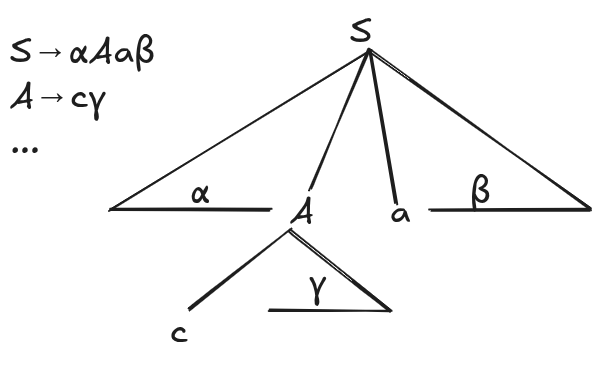
\includegraphics[width=0.6\linewidth,height=\textheight,keepaspectratio]{chapters/images/first-follow.png}

}

\caption{\label{fig-firstfollow}Ilustração para os conjuntos
First/Follow}

\end{figure}%

\subsubsection{\texorpdfstring{Função
\(FIRST\)}{Função FIRST}}\label{funuxe7uxe3o-first}

A função \(FIRST\) determina quais símbolos terminais podem aparecer
como primeiro símbolo de uma cadeia derivada a partir de um determinado
símbolo da gramática. Além dos terminais, o conjunto \(FIRST\) pode
conter o símbolo \(\lambda\), indicando que o símbolo analisado pode
derivar a cadeia vazia. O cálculo deve ser realizado para todos os
símbolos da gramática e repetido até que nenhum novo elemento possa ser
acrescentado a qualquer conjunto \(FIRST\).

Inicialmente, considere um símbolo \(X\) que seja terminal. Nesse caso,
o primeiro símbolo de uma cadeia iniciada por \(X\) é necessariamente o
próprio \(X\). Portanto, seu conjunto \(FIRST\) é formado exclusivamente
pelo próprio símbolo terminal, isto é, \(FIRST(X)=\{X\}\). Por exemplo,
se \(a\) é um terminal da gramática, então \(FIRST(a)=\{a\}\).

Para um símbolo \(X\) que seja não terminal, é necessário analisar cada
uma das produções que possuem \(X\) como lado esquerdo. Considere, por
exemplo, uma produção da forma \(X\rightarrow Y_1Y_2\ldots Y_k\), em que
\(k\geq1\). O primeiro símbolo que pode ser produzido a partir de \(X\)
depende inicialmente de \(Y_1\). Assim, todos os terminais pertencentes
a \(FIRST(Y_1)\), exceto \(\lambda\), devem ser acrescentados a
\(FIRST(X)\).

Entretanto, existe uma situação que exige uma análise adicional. Se
\(\lambda\) pertence a \(FIRST(Y_1)\), significa que \(Y_1\) pode
desaparecer durante a derivação, produzindo a cadeia vazia. Nesse caso,
o primeiro símbolo da cadeia derivada de \(X\) poderá vir de \(Y_2\).
Portanto, os elementos de \(FIRST(Y_2)\), exceto \(\lambda\), também
devem ser acrescentados a \(FIRST(X)\). Esse processo continua
sucessivamente: se \(\lambda\) pertence a \(FIRST(Y_2)\), deve-se
considerar \(Y_3\), e assim por diante.

De maneira geral, para uma produção \(X\rightarrow Y_1Y_2\ldots Y_k\),
um terminal \(a\) deve ser acrescentado a \(FIRST(X)\) se \(a\) pertence
a \(FIRST(Y_i)\) para algum \(i\), desde que todos os símbolos
anteriores \(Y_1,\ldots,Y_{i-1}\) possam derivar \(\lambda\). Em outras
palavras, para que um símbolo pertencente a \(FIRST(Y_i)\) possa ser o
primeiro símbolo derivado de \(X\), todos os símbolos que o precedem na
produção precisam ter a possibilidade de desaparecer.

Há ainda um caso especial quando todos os símbolos da produção podem
derivar \(\lambda\). Se \(\lambda\) pertence a \(FIRST(Y_j)\) para todo
\(j=1,2,\ldots,k\), então toda a sequência \(Y_1Y_2\ldots Y_k\) pode
derivar a cadeia vazia. Consequentemente, \(\lambda\) deve ser
acrescentado a \(FIRST(X)\). Por exemplo, se \(X\rightarrow ABC\) e
\(\lambda\in FIRST(A)\), \(\lambda\in FIRST(B)\) e
\(\lambda\in FIRST(C)\), então \(\lambda\in FIRST(X)\).

Finalmente, quando existe diretamente uma produção da forma
\(X\rightarrow\lambda\), o símbolo \(X\) pode produzir a cadeia vazia
sem a necessidade de realizar qualquer outra derivação. Nesse caso,
\(\lambda\) deve ser acrescentado imediatamente ao conjunto
\(FIRST(X)\).

O cálculo de \(FIRST\) é, portanto, iterativo. Os conjuntos são
inicialmente construídos a partir dos terminais e das produções que
permitem derivar \(\lambda\). Em seguida, as produções são examinadas
repetidamente para propagar os símbolos terminais e \(\lambda\) entre os
conjuntos \(FIRST\). O processo termina quando uma nova passagem por
todas as produções não acrescenta nenhum elemento a nenhum conjunto.
Nesse momento, diz-se que os conjuntos \(FIRST\) atingiram um ponto
fixo, e seus conteúdos representam todos os possíveis primeiros símbolos
das cadeias que podem ser derivadas a partir dos símbolos da gramática.

\begin{tcolorbox}[enhanced jigsaw, toptitle=1mm, rightrule=.15mm, title=\textcolor{quarto-callout-note-color}{\faInfo}\hspace{0.5em}{Resumo do Cálculo de FIRST}, toprule=.15mm, colback=white, left=2mm, arc=.35mm, opacitybacktitle=0.6, colframe=quarto-callout-note-color-frame, breakable, coltitle=black, titlerule=0mm, bottomtitle=1mm, leftrule=.75mm, bottomrule=.15mm, opacityback=0, colbacktitle=quarto-callout-note-color!10!white]

Para calcular \(FIRST\) de todos os simbolos \(X\) de uma gramática,
execute as seguintes regras até que nenhum novo símbolo possa ser
acrescentado a qualquer conjunto \(FIRST\).

\begin{enumerate}
\def\labelenumi{\arabic{enumi}.}
\item
  Se \(X\) é um símbolo terminal, então \(FIRST(X) = \{X\}\)
\item
  Se \(X\) é um não-terminal e \(X\rightarrow Y_1Y_2...Y_k\) é uma regra
  de produção para algum \(k \geq 1\), então acrescente \(a\) a
  \(FIRST(X)\) se, para algum \(i\), \(a\) estiver em \(FIRST(Y_i)\), e
  \(\lambda\) estiver em todos os \(FIRST(Y_1),...,FIRST(Y_{i-1})\). Se
  \(\lambda\) está em \(FIRST(Y_j)\) para todo \(j=1,2,...,k\), então
  adicione \(\lambda\) a \(FIRST(X)\).
\item
  Se \(X \rightarrow \lambda\) é um regra de produção, então acrescente
  \(\lambda\) a \(FIRST(X)\)
\end{enumerate}

\end{tcolorbox}

\subsubsection{\texorpdfstring{Função
\(FOLLOW\)}{Função FOLLOW}}\label{funuxe7uxe3o-follow}

A função \(FOLLOW\) determina quais símbolos podem aparecer
\textbf{imediatamente após um determinado não terminal} em uma cadeia
derivada da gramática. Diferentemente da função \(FIRST\), que está
relacionada aos símbolos que podem iniciar uma derivação, a função
\(FOLLOW\) considera os símbolos que podem suceder um não terminal. O
cálculo de \(FOLLOW\) é realizado para todos os símbolos não terminais
da gramática e utiliza os conjuntos \(FIRST\) previamente calculados.

O primeiro passo consiste em considerar o símbolo inicial da gramática.
Seja \(S\) o símbolo inicial. Como uma sentença completa deve ser
seguida pelo marcador de fim de sentença, representado por \(\#\), esse
símbolo é acrescentado inicialmente ao conjunto \(FOLLOW(S)\). Assim,
temos:

\[
\# \in FOLLOW(S)
\]

O marcador \(\#\) representa o fim da entrada e é considerado como
estando após toda a sentença durante o processo de análise. Portanto,
quando o analisador sintático alcançar o final da cadeia de entrada,
esse marcador permite identificar que não existem mais símbolos a serem
processados.

Considere agora uma produção da forma \(A\rightarrow\alpha B\beta\), na
qual \(B\) é um não terminal e \(\beta\) representa a sequência de
símbolos que aparece imediatamente após \(B\). Nesse caso, todos os
símbolos de \(FIRST(\beta)\), com exceção de \(\lambda\), devem ser
acrescentados a \(FOLLOW(B)\). Isso ocorre porque qualquer terminal que
possa iniciar uma cadeia derivada de \(\beta\) poderá aparecer
imediatamente depois de \(B\) durante uma derivação.

Por exemplo, considere a produção:

\[
A\rightarrow \alpha Bcd
\]

Como a sequência que sucede \(B\) começa pelo terminal \(c\), temos
\(c\in FIRST(cd)\). Consequentemente, \(c\) deve ser incluído em
\(FOLLOW(B)\). O mesmo princípio se aplica quando \(\beta\) é formada
por vários símbolos e seu primeiro símbolo pode desaparecer por
derivação de \(\lambda\).

Existe ainda uma situação importante quando a sequência \(\beta\) pode
derivar \(\lambda\). Considere novamente uma produção da forma
\(A\rightarrow\alpha B\beta\). Se \(\lambda\in FIRST(\beta)\), então
\(\beta\) pode desaparecer durante a derivação. Nesse caso, os símbolos
que podem aparecer depois de \(A\) também podem aparecer imediatamente
depois de \(B\). Portanto, todos os elementos de \(FOLLOW(A)\) devem ser
acrescentados a \(FOLLOW(B)\).

O mesmo raciocínio se aplica quando \(B\) aparece no final da produção,
isto é, em uma produção da forma \(A\rightarrow\alpha B\). Como não
existe nenhum símbolo depois de \(B\) nessa produção, tudo aquilo que
pode aparecer depois de \(A\) também poderá aparecer depois de \(B\).
Assim, os elementos de \(FOLLOW(A)\) devem ser incluídos em
\(FOLLOW(B)\).

O cálculo de \(FOLLOW\) é, portanto, um processo \textbf{iterativo}.
Inicialmente, coloca-se \(\#\) no conjunto \(FOLLOW\) do símbolo
inicial. Em seguida, percorrem-se todas as produções, aplicando as
regras de propagação dos símbolos obtidos a partir de \(FIRST\) e dos
conjuntos \(FOLLOW\) dos não terminais. Como uma informação obtida em
uma produção pode gerar novas informações em outra produção, as regras
precisam ser executadas repetidamente.

O processo termina quando uma nova passagem por todas as produções não
acrescenta nenhum novo símbolo a nenhum conjunto \(FOLLOW\). Nesse
momento, os conjuntos atingiram um \textbf{ponto fixo} e contêm todos os
símbolos que podem aparecer imediatamente após cada não terminal em
alguma derivação possível da gramática.

A função \(FOLLOW(B)\) determina os símbolos que podem aparecer
imediatamente após o não terminal \(B\) em alguma cadeia derivada da
gramática.

Para o símbolo inicial \(S\), acrescenta-se inicialmente o marcador de
fim de sentença \(\#\):

\[
\#\in FOLLOW(S)
\]

Para uma produção \(A\rightarrow\alpha B\beta\), todos os símbolos de
\(FIRST(\beta)\), exceto \(\lambda\), são acrescentados a \(FOLLOW(B)\):

\[
FIRST(\beta)-\{\lambda\}\subseteq FOLLOW(B)
\]

Se \(\beta\) puder derivar \(\lambda\), ou se \(B\) estiver no final da
produção, os símbolos de \(FOLLOW(A)\) também devem ser acrescentados a
\(FOLLOW(B)\):

\[
FOLLOW(A)\subseteq FOLLOW(B)
\]

As regras são aplicadas repetidamente a todas as produções até que
nenhum novo símbolo possa ser acrescentado aos conjuntos. O resultado
final corresponde ao \textbf{ponto fixo dos conjuntos \(FOLLOW\)} da
gramática.

\begin{tcolorbox}[enhanced jigsaw, toptitle=1mm, rightrule=.15mm, title=\textcolor{quarto-callout-note-color}{\faInfo}\hspace{0.5em}{Resumo do Cálculo de FOLLOW}, toprule=.15mm, colback=white, left=2mm, arc=.35mm, opacitybacktitle=0.6, colframe=quarto-callout-note-color-frame, breakable, coltitle=black, titlerule=0mm, bottomtitle=1mm, leftrule=.75mm, bottomrule=.15mm, opacityback=0, colbacktitle=quarto-callout-note-color!10!white]

Para calcular \(FOLLOW\) de todos os simbolos NÃO-TERMINAIS \(S\) de uma
gramática, execute as seguintes regras até que nenhum novo símbolo possa
ser acrescentado a qualquer conjunto \(FOLLOW\).

\begin{enumerate}
\def\labelenumi{\arabic{enumi}.}
\item
  Coloque \(\#\) em \(FOLLOW(S)\), onde \(S\) é o símbolo inicial da
  gramática e \(\#\) é o marcador de fim de sentença, que é incluido
  antes da avaliação da sentença.
\item
  Se houver uma produção \(A \rightarrow \alpha B \beta\), então tudo
  que está em \(FIRST(\beta)\) exceto \(\lambda\), deve estar em
  \(FOLLOW(B)\).
\item
  Se houver uma produção \(A \rightarrow \alpha B\) ou
  \(A \rightarrow \alpha B \beta\), onde \(FIRST(\beta)\) contém
  \(\lambda\), então inclua \(FOLLOW(A)\) em \(FOLLOW(B)\).
\end{enumerate}

\end{tcolorbox}

\ul{\textbf{Exemplo:}}

Considere a seguinte gramática:

\(E \rightarrow TE^{'}\)

\(E^{'} \rightarrow +TE^{'} | \lambda\)

\(T \rightarrow FT^{'}\)

\(T^{'} \rightarrow *FT^{'} | \lambda\)

\(F \rightarrow a | (E)\)

\ul{\textbf{Conjuntos FIRST e FOLLOW:}}

\begin{longtable*}[]{|l|c|c|}
\toprule\noalign{}
& FIRST & FOLLOW \\
\midrule\noalign{}
\endhead
\bottomrule\noalign{}
\endlastfoot
\(E\) & \(\{(, a\}\) & \(\{), \#\}\) \\
\midrule
\(E'\) & \(\{+, \lambda\}\) & \(\{), \#\}\) \\
\midrule
\(T\) & \(\{(, a\}\) & \(\{+, ), \#\}\) \\
\midrule
\(T'\) & \(\{*, \lambda\}\) & \(\{+, ), \#\}\) \\
\midrule
\(F\) & \(\{(, a\}\) & \(\{*, +, ), \#\}\) \\
\end{longtable*}

\subsubsection{Tabela de Análise Preditiva
LL(1)}\label{tabela-de-anuxe1lise-preditiva-ll1}

A construção da \textbf{tabela de análise preditiva LL(1)} constitui uma
etapa fundamental para a implementação de um analisador sintático
descendente preditivo. A tabela estabelece, para cada combinação entre
um \textbf{não terminal da gramática} e um \textbf{terminal da entrada},
qual produção deve ser utilizada durante a análise. Dessa forma, o
analisador pode determinar a produção a ser aplicada sem realizar
retrocesso ou testar diferentes alternativas.

A construção da tabela utiliza diretamente as informações obtidas pelos
conjuntos \textbf{\(FIRST\)} e \textbf{\(FOLLOW\)} da gramática. O
conjunto \(FIRST\) permite identificar quais terminais podem iniciar uma
cadeia derivada a partir do lado direito de uma produção. Já o conjunto
\(FOLLOW\) é utilizado quando essa cadeia pode derivar a palavra vazia
\(\lambda\), indicando que a produção pode ser escolhida com base no
símbolo que aparece imediatamente após o não terminal analisado.

Considere uma produção \(A\rightarrow\alpha\). Inicialmente, devem ser
considerados todos os terminais pertencentes a \(FIRST(\alpha)\). Para
cada terminal \(a\in FIRST(\alpha)\), a produção \(A\rightarrow\alpha\)
é inserida na posição \(T[A,a]\) da tabela. Isso significa que, quando o
analisador estiver considerando o não terminal \(A\) e o próximo símbolo
da entrada for \(a\), a produção \(A\rightarrow\alpha\) poderá ser
utilizada.

Entretanto, existe uma situação particular quando \(\alpha\) pode
derivar a palavra vazia. Nesse caso, \(\lambda\in FIRST(\alpha)\), e não
existe necessariamente um terminal de \(FIRST(\alpha)\) que determine
diretamente a escolha da produção. A decisão passa então a depender dos
símbolos que podem aparecer imediatamente depois de \(A\). Por isso,
para cada terminal \(b\in FOLLOW(A)\), a produção \(A\rightarrow\alpha\)
é inserida na posição \(T[A,b]\).

Assim, a construção da tabela pode ser entendida como uma combinação das
informações fornecidas por \(FIRST\) e \(FOLLOW\): \textbf{\(FIRST\)}
determina os terminais que podem iniciar a derivação do lado direito da
produção, enquanto \textbf{\(FOLLOW\)} determina os terminais que
permitem selecionar uma produção quando seu lado direito pode
desaparecer por meio de uma derivação para \(\lambda\).

O algoritmo percorre todas as produções da gramática e preenche
progressivamente as células da tabela. Ao final do processo, cada célula
\(T[A,a]\) indica a produção que deve ser utilizada quando o topo da
pilha contém o não terminal \(A\) e o próximo símbolo da entrada é o
terminal \(a\). Para uma gramática LL(1), cada célula da tabela deve
conter \textbf{no máximo uma produção}. Caso duas ou mais produções
diferentes sejam inseridas na mesma célula, existe um conflito,
indicando que a gramática não possui uma tabela de análise preditiva
LL(1) determinística para aquela situação.

\subsubsection{Algoritmo para construir a Tabela de Análise Preditiva
LL(1)}\label{algoritmo-para-construir-a-tabela-de-anuxe1lise-preditiva-ll1}

Para cada produção \(A\rightarrow\alpha\) da gramática, são aplicadas as
seguintes regras:

\begin{enumerate}
\def\labelenumi{\arabic{enumi}.}
\item
  Para cada terminal \(a\in FIRST(\alpha)\), \textbf{exceto
  \(\lambda\)}, adiciona-se a produção \(A\rightarrow\alpha\) à posição
  \(T[A,a]\).
\item
  Se \(\lambda\in FIRST(\alpha)\), então, para cada terminal
  \(b\in FOLLOW(A)\), adiciona-se a produção \(A\rightarrow\alpha\) à
  posição \(T[A,b]\).
\end{enumerate}

Dessa maneira, a tabela fornece ao analisador uma forma direta de
selecionar a produção adequada a partir de apenas dois elementos:
\textbf{o não terminal que está no topo da pilha e o próximo terminal da
entrada}. Isso caracteriza o princípio fundamental da análise
\textbf{LL(1)}: a entrada é lida da esquerda para a direita, produz-se
uma derivação mais à esquerda e utiliza-se apenas \textbf{um símbolo de
antecipação} (\emph{lookahead}) para determinar a produção a ser
aplicada.

A tabela LL(1) preditiva para a gramática de expressões sem recursão à
esquerda apresentada anteriormente, é:

\begin{longtable}[]{|
  >{\centering\arraybackslash}p{(\linewidth - 14\tabcolsep - 8\arrayrulewidth) * \real{0.1176}}|
  >{\centering\arraybackslash}p{(\linewidth - 14\tabcolsep - 8\arrayrulewidth) * \real{0.1471}}|
  >{\centering\arraybackslash}p{(\linewidth - 14\tabcolsep - 8\arrayrulewidth) * \real{0.1471}}|
  >{\centering\arraybackslash}p{(\linewidth - 14\tabcolsep - 8\arrayrulewidth) * \real{0.1471}}|
  >{\centering\arraybackslash}p{(\linewidth - 14\tabcolsep - 8\arrayrulewidth) * \real{0.1471}}|
  >{\centering\arraybackslash}p{(\linewidth - 14\tabcolsep - 8\arrayrulewidth) * \real{0.1471}}|
  >{\centering\arraybackslash}p{(\linewidth - 14\tabcolsep - 8\arrayrulewidth) * \real{0.1471}}|}

\caption{\label{tbl-tabela-ll1}Tabela de análise preditiva LL(1)}

\tabularnewline

\toprule\noalign{}
\begin{minipage}[b]{\linewidth}\smallskip
\centering
\end{minipage} & \begin{minipage}[b]{\linewidth}\centering
\(a\)
\end{minipage} & \begin{minipage}[b]{\linewidth}\centering
\(+\)
\end{minipage} & \begin{minipage}[b]{\linewidth}\centering
\(*\)
\end{minipage} & \begin{minipage}[b]{\linewidth}\centering
\((\)
\end{minipage} & \begin{minipage}[b]{\linewidth}\centering
\()\)
\end{minipage} & \begin{minipage}[b]{\linewidth}\centering
\(\#\)
\end{minipage} \\
\midrule\noalign{}
\endhead
\bottomrule\noalign{}
\endlastfoot
\(E\) & \(E \rightarrow TE'\) & & & \(E \rightarrow TE'\) & & \\
\midrule
\(E'\) & & \(E' \rightarrow +TE'\) & & & \(E' \rightarrow \lambda\) &
\(E' \rightarrow \lambda\) \\
\midrule
\(T\) & \(T \rightarrow FT'\) & & & \(T \rightarrow FT'\) & & \\
\midrule
\(T'\) & & \(T' \rightarrow \lambda\) & \(T' \rightarrow *FT'\) & &
\(T' \rightarrow \lambda\) & \(T' \rightarrow \lambda\) \\
\midrule
\(F\) & \(F \rightarrow a\) & & & \(F \rightarrow (E)\) & & \\

\end{longtable}

\subsubsection{Exemplo de derivação utilizando a tabela
preditiva}\label{exemplo-de-derivauxe7uxe3o-utilizando-a-tabela-preditiva}

Considere a Tabela~\ref{tbl-tabela-ll1} e a sentença:

\[
(a+a)*a
\]

A derivação da sentença pode ser realizada a partir do símbolo inicial
\(E\), sempre expandindo o \textbf{não terminal mais à esquerda}. A
produção a ser utilizada em cada etapa é determinada pelo não terminal
que está sendo analisado e pelo próximo símbolo da entrada
(\emph{lookahead}).

A sequência de derivações para obter a sentença \((a+a)*a\) é:

\[
\begin{aligned}
E
&\Rightarrow TE'\\
&\Rightarrow FT'E'\\
&\Rightarrow (E)T'E'\\
&\Rightarrow (TE')T'E'\\
&\Rightarrow (FT'E')T'E'\\
&\Rightarrow (aT'E')T'E'\\
&\Rightarrow (aE')T'E'\\
&\Rightarrow (a+TE')T'E'\\
&\Rightarrow (a+FT'E')T'E'\\
&\Rightarrow (a+aT'E')T'E'\\
&\Rightarrow (a+aE')T'E'\\
&\Rightarrow (a+a)T'E'\\
&\Rightarrow (a+a)*FT'E'\\
&\Rightarrow (a+a)*aT'E'\\
&\Rightarrow (a+a)*aE'\\
&\Rightarrow (a+a)*a
\end{aligned}
\]

A derivação começa com o símbolo inicial \(E\). Como o primeiro símbolo
da sentença é o terminal \texttt{(}, a tabela preditiva determina a
utilização da produção \(E\rightarrow TE'\). Em seguida, o não terminal
\(T\) é analisado e, como o próximo símbolo continua sendo \texttt{(},
utiliza-se \(T\rightarrow FT'\).

Para o não terminal \(F\), o símbolo de antecipação também é \texttt{(}.
Portanto, a tabela determina a produção \(F\rightarrow(E)\). Dessa
maneira, a análise passa a considerar o conteúdo existente entre os
parênteses.

Dentro dos parênteses, o próximo símbolo é novamente \texttt{(}? Não. O
primeiro símbolo é \(a\). Assim, para o não terminal \(E\), utiliza-se
\(E\rightarrow TE'\), e para \(T\) utiliza-se \(T\rightarrow FT'\). Como
o próximo símbolo é \(a\), a produção selecionada para \(F\) é
\(F\rightarrow a\).

Após reconhecer o primeiro \(a\), o próximo símbolo da entrada é
\texttt{+}. Nesse momento, para o não terminal \(E'\), a tabela indica a
produção:

\[
E'\rightarrow +TE'
\]

O símbolo \texttt{+} é, portanto, reconhecido e o não terminal \(T\)
passa a ser analisado para reconhecer o segundo operando da soma. Como o
próximo símbolo é \(a\), são utilizadas as produções:

\[
T\rightarrow FT'
\]

e

\[
F\rightarrow a.
\]

Após o reconhecimento do segundo \(a\), o próximo símbolo da entrada é
\texttt{)}. Como \()\) pertence a \(FOLLOW(E')\), a tabela preditiva
determina a utilização da produção:

\[
E'\rightarrow\lambda.
\]

Dessa forma, o conteúdo entre parênteses é concluído, resultando em:

\[
(a+a).
\]

Após o fechamento dos parênteses, o próximo símbolo da entrada é
\texttt{*}. O não terminal \(T'\) encontra-se então no topo da derivação
e, consultando a tabela preditiva, utiliza-se a produção:

\[
T'\rightarrow *FT'.
\]

O símbolo \texttt{*} é reconhecido e, em seguida, \(F\) é utilizado para
reconhecer o próximo operando. Como o próximo símbolo é \(a\),
aplica-se:

\[
F\rightarrow a.
\]

Depois do reconhecimento do último \(a\), o próximo símbolo é o marcador
de fim de sentença \(\#\). Nesse caso, tanto \(T'\) quanto \(E'\) podem
ser substituídos por \(\lambda\), utilizando as produções:

\[
T'\rightarrow\lambda
\]

e

\[
E'\rightarrow\lambda.
\]

A derivação é concluída quando todos os símbolos não terminais são
eliminados e toda a entrada é reconhecida. Assim, obtém-se:

\[
\boxed{E\Rightarrow^*(a+a)*a}
\]

O exemplo mostra como a tabela preditiva LL(1) permite determinar, de
forma determinística, a produção a ser utilizada em cada etapa da
análise. A decisão depende apenas do \textbf{não terminal no topo da
pilha} e do \textbf{próximo símbolo da entrada}, isto é, de um único
símbolo de antecipação (\emph{lookahead}).

A seguinte definição permite identificar as gramáticas LL(1):

\begin{definition}[]\protect\hypertarget{def-gll}{}\label{def-gll}

Uma gramática G não recursiva à esquerda é LL(1)se e somente se, sempre
que \(A \rightarrow \alpha\) e \(A \rightarrow \beta\) são regras de
produção de G, ocorre que:

\begin{enumerate}
\def\labelenumi{\arabic{enumi}.}
\item
  a interseção dos conjuntos \(FIRST(\alpha)\) e \(FIRST(\beta)\) é
  vazia;
\item
  no máximo um dos dois, \(\alpha\) ou \(\beta\), deriva a palavra
  vazia; e
\item
  se \(\beta \overset{*}{\Rightarrow} \lambda\), então a interseção de
  \(FIRST(\alpha)\) e \(FOLLOW(A)\) é vazia;
\end{enumerate}

\end{definition}

\subsection{Análise sintática LR}\label{anuxe1lise-sintuxe1tica-lr}

Os analisadores sintáticos ascendentes, também denominados analisadores
\emph{bottom-up}, realizam a construção da árvore sintática partindo dos
símbolos da cadeia de entrada e progredindo em direção ao símbolo
inicial da gramática. Enquanto os analisadores descendentes procuram
construir a sentença a partir do símbolo inicial, os analisadores
ascendentes realizam o processo inverso: começam pela sentença e
procuram reconstruir, por meio de reduções, a derivação que levou à sua
geração.

Uma importante classe de analisadores ascendentes é formada pelos
analisadores \textbf{LR}. A denominação LR possui um significado
específico. A letra \textbf{L} (\emph{Left-to-right}) indica que a
cadeia de entrada é examinada da \textbf{esquerda para a direita}.
Portanto, diferentemente do que poderia sugerir a expressão ``análise
ascendente'', a entrada não é percorrida da direita para a esquerda.

A letra \textbf{R} (\emph{Rightmost}) está relacionada à derivação mais
à direita. Mais precisamente, um analisador LR reconstrói, em ordem
inversa, uma \textbf{derivação mais à direita} da sentença. Assim,
enquanto uma derivação convencional parte do símbolo inicial e substitui
sucessivamente o não terminal mais à direita, o analisador LR parte da
sentença e realiza reduções que desfazem essas substituições.

O número associado ao analisador, como em \textbf{LR(1)}, indica a
quantidade de símbolos de antecipação (\emph{lookahead}) utilizados para
tomar as decisões de análise. No caso do LR(1), cada decisão é realizada
considerando o próximo símbolo da cadeia de entrada. Existem diferentes
famílias de analisadores LR, como LR(0), SLR(1), LALR(1) e LR(1), que
diferem principalmente na forma como os estados e as informações de
antecipação são construídos e utilizados.

\subsubsection{A ideia da análise
ascendente}\label{a-ideia-da-anuxe1lise-ascendente}

A ideia fundamental de uma análise ascendente pode ser compreendida
considerando uma sentença \(\alpha\) pertencente à linguagem gerada por
uma gramática. O objetivo do analisador é reduzir progressivamente essa
sentença até obter o símbolo inicial da gramática.

Considere uma sentença representada pela cadeia:

\[
\alpha = \beta X_1X_2\ldots X_n\gamma
\]

e suponha que exista uma produção da gramática da forma:

\[
X\rightarrow X_1X_2\ldots X_n.
\]

Se a sequência \(X_1X_2\ldots X_n\) corresponde ao lado direito de uma
produção e representa uma parte da derivação que pode ser substituída
por \(X\), o analisador pode realizar a redução:

\[
\beta X_1X_2\ldots X_n\gamma
\Rightarrow
\beta X\gamma.
\]

Esse processo corresponde à operação inversa de uma etapa de derivação.
Na derivação, o não terminal \(X\) seria substituído por
\(X_1X_2\ldots X_n\):

\[
X\Rightarrow X_1X_2\ldots X_n.
\]

Na análise ascendente, realiza-se justamente o caminho inverso:

\[
X_1X_2\ldots X_n\Rightarrow X.
\]

Essa operação é denominada \textbf{redução}. Durante a redução, a
sequência de símbolos \(X_1X_2\ldots X_n\) é reconhecida como uma
instância do lado direito de uma produção e é substituída pelo seu lado
esquerdo, o não terminal \(X\).

A operação de redução pode também ser interpretada graficamente como a
construção de uma parte da árvore sintática. Os símbolos
\(X_1,X_2,\ldots,X_n\) correspondem aos filhos do nó \(X\). Ao realizar
a redução, esses símbolos são agrupados sob um novo nó cuja raiz é
\(X\).

O processo de análise ascendente continua realizando operações desse
tipo até que toda a sentença tenha sido reduzida ao símbolo inicial da
gramática. Quando isso ocorre, significa que a cadeia de entrada pode
ser derivada pela gramática e, portanto, pertence à linguagem gerada por
ela.

\subsubsection{O problema da escolha da
redução}\label{o-problema-da-escolha-da-reduuxe7uxe3o}

Na descrição genérica da análise ascendente, pode parecer simples
identificar uma sequência de símbolos que corresponde ao lado direito de
uma produção e substituí-la pelo respectivo não terminal. Entretanto,
durante uma análise real, podem existir várias possibilidades de
redução.

Considere, por exemplo, uma situação em que diferentes sequências de
símbolos presentes na pilha correspondam ao lado direito de diferentes
produções. O analisador precisa determinar qual delas deve ser reduzida
e, em determinadas situações, pode ser necessário decidir também se deve
realizar uma redução ou continuar lendo símbolos da entrada.

Essa decisão não pode ser feita simplesmente procurando uma produção que
corresponda aos símbolos presentes na pilha. É necessário considerar o
\textbf{contexto da análise} e o próximo símbolo da entrada. Os
analisadores LR automatizam esse processo utilizando uma estrutura de
estados e uma tabela de análise.

A tabela permite determinar, para cada estado do analisador e para cada
símbolo relevante da gramática, qual ação deve ser executada. Dessa
maneira, o processo de análise deixa de depender de decisões intuitivas
e passa a ser conduzido de forma determinística por meio de um conjunto
finito de estados e ações.

\subsubsection{Pilha e tabela de
análise}\label{pilha-e-tabela-de-anuxe1lise}

Durante a análise LR, o analisador mantém uma \textbf{pilha} que
representa o estado atual da análise. Os estados são utilizados para
registrar informações sobre os símbolos que já foram reconhecidos e
sobre as possíveis continuações da derivação.

A cada etapa, o analisador considera o estado que se encontra no topo da
pilha e o próximo símbolo da cadeia de entrada. A partir dessa
combinação, uma consulta é realizada na tabela de análise. O conteúdo da
célula determina a ação que deve ser executada.

De maneira simplificada, o funcionamento pode ser descrito da seguinte
forma:

\begin{enumerate}
\def\labelenumi{\arabic{enumi}.}
\item
  O analisador inicia no estado inicial e coloca esse estado na pilha.
\item
  O próximo símbolo da cadeia de entrada é utilizado juntamente com o
  estado no topo da pilha para consultar a tabela de análise.
\item
  A tabela determina a ação que deve ser realizada.
\item
  Se a ação for um \textbf{deslocamento}, um novo estado é colocado na
  pilha e o símbolo correspondente é consumido da entrada.
\item
  Se a ação for uma \textbf{redução}, os estados correspondentes ao lado
  direito de uma produção são retirados da pilha e o não terminal do
  lado esquerdo é considerado para determinar o próximo estado.
\item
  O processo continua até que a entrada seja aceita ou seja identificada
  uma situação de erro.
\end{enumerate}

A tabela de análise pode ser entendida como uma matriz retangular cujas
linhas correspondem aos estados do analisador e cujas colunas
correspondem aos símbolos da gramática. Dependendo da organização
adotada, as colunas podem ser divididas em símbolos terminais,
associados às ações de análise, e símbolos não terminais, associados às
transições entre estados.

As principais ações encontradas em uma tabela de análise LR são:

\begin{itemize}
\tightlist
\item
  \textbf{Deslocamento (\emph{shift})}: o próximo símbolo da entrada é
  reconhecido e um novo estado é colocado na pilha.
\item
  \textbf{Redução (\emph{reduce})}: uma sequência de símbolos já
  reconhecida é substituída pelo não terminal correspondente ao lado
  esquerdo de uma produção.
\item
  \textbf{Aceitação (\emph{accept})}: indica que toda a entrada foi
  reconhecida e que a sentença pertence à linguagem da gramática.
\item
  \textbf{Erro (\emph{error})}: indica que não existe uma ação válida
  para a combinação entre o estado atual e o símbolo de entrada.
\end{itemize}

\subsubsection{Exemplo de uma tabela de análise
LR}\label{exemplo-de-uma-tabela-de-anuxe1lise-lr}

Considere a seguinte gramática, cujas produções foram numeradas para
facilitar sua identificação durante o processo de análise:

\[
\begin{array}{rrcl}
(1) & E & \rightarrow & +EE\\
(2) & E & \rightarrow & *EE\\
(3) & E & \rightarrow & a\\
(4) & E & \rightarrow & b
\end{array}
\]

Essa gramática gera expressões em uma notação prefixada. As produções
(3) e (4) permitem gerar os operandos \(a\) e \(b\), enquanto as
produções (1) e (2) permitem construir expressões utilizando os
operadores \(+\) e \(*\).

Para essa gramática, considere a seguinte tabela simplificada de análise
LR:

\begin{longtable}[]{|c|c|c|c|c|c|c|}

\caption{\label{tbl-analise-lr}Tabela de análise LR}

\tabularnewline

\toprule\noalign{}
Estado & \(E\) & \(+\) & \(*\) & \(a\) & \(b\) & \(\#\) \\
\midrule\noalign{}
\endhead
\bottomrule\noalign{}
\endlastfoot
\(e_0\) & \(e_1\) & \(e_2\) & \(e_3\) & \(e_4\) & \(e_5\) & \\
\midrule
\(e_1\) & & & & & & \(a\) \\
\midrule
\(e_2\) & \(e_6\) & \(e_2\) & \(e_3\) & \(e_4\) & \(e_5\) & \\
\midrule
\(e_3\) & \(e_7\) & \(e_2\) & \(e_3\) & \(e_4\) & \(e_5\) & \\
\midrule
\(e_4\) & & \(r_3\) & \(r_3\) & \(r_3\) & \(r_3\) & \(r_3\) \\
\midrule
\(e_5\) & & \(r_4\) & \(r_4\) & \(r_4\) & \(r_4\) & \(r_4\) \\
\midrule
\(e_6\) & \(e_8\) & \(e_2\) & \(e_3\) & \(e_4\) & \(e_5\) & \\
\midrule
\(e_7\) & \(e_9\) & \(e_2\) & \(e_3\) & \(e_4\) & \(e_5\) & \\
\midrule
\(e_8\) & & \(r_1\) & \(r_1\) & \(r_1\) & \(r_1\) & \(r_1\) \\
\midrule
\(e_9\) & & \(r_2\) & \(r_2\) & \(r_2\) & \(r_2\) & \(r_2\) \\

\end{longtable}

O símbolo \(\#\) é utilizado como \textbf{marcador de fim da entrada}.
Ele não pertence aos símbolos da linguagem; sua função é indicar ao
analisador que todos os símbolos da sentença já foram fornecidos. Assim,
quando o analisador encontra \(\#\) em uma situação apropriada, pode
determinar que a análise chegou ao final.

Na tabela apresentada, as entradas \(e_i\) representam estados do
analisador. As entradas \(r_j\) representam operações de redução
utilizando a produção de número \(j\). A entrada \(a\) representa a ação
de aceitação. Uma célula vazia representa uma situação para a qual não
existe uma ação válida e, portanto, corresponde a uma situação de erro.

Assim, as ações da tabela podem ser interpretadas da seguinte maneira:

\begin{itemize}
\tightlist
\item
  \(e_i\): deslocar para o estado \(e_i\) (\emph{shift});
\item
  \(r_j\): realizar uma redução utilizando a produção \(j\);
\item
  \(a\): aceitar a cadeia de entrada;
\item
  célula vazia: erro de análise.
\end{itemize}

\subsubsection{Funcionamento do
analisador}\label{funcionamento-do-analisador}

Considerando a tabela anterior, o algoritmo de análise pode ser descrito
como um processo iterativo no qual o analisador mantém três informações
principais: a \textbf{pilha de estados}, a \textbf{cadeia de entrada} e
a \textbf{tabela de análise}.

Inicialmente, a pilha contém apenas o estado inicial \(e_0\). O
analisador consulta o primeiro símbolo da entrada e utiliza a combinação
entre esse símbolo e o estado no topo da pilha para determinar a próxima
ação.

Quando a tabela determina um deslocamento, o analisador reconhece o
símbolo atual da entrada e avança para o estado indicado pela tabela.
Esse novo estado é colocado na pilha. O símbolo da entrada que foi
consumido deixa de ser considerado como o próximo símbolo de entrada.

Quando a tabela determina uma redução \(r_j\), o analisador identifica
que uma sequência de símbolos já reconhecida corresponde ao lado direito
da produção de número \(j\). Essa sequência é retirada da pilha e
substituída conceitualmente pelo não terminal que aparece no lado
esquerdo da produção. Em seguida, o analisador consulta a parte
correspondente aos não terminais da tabela para determinar o próximo
estado.

A operação de redução é justamente o mecanismo que permite ao analisador
construir a árvore sintática \textbf{de baixo para cima}. Cada redução
reconhece uma subestrutura da árvore e a transforma em um único não
terminal. Reduções sucessivas fazem com que estruturas menores sejam
combinadas em estruturas cada vez maiores, até que toda a sentença seja
representada pelo símbolo inicial \(E\).

O analisador continua alternando entre operações de deslocamento e
redução. O deslocamento permite avançar sobre a cadeia de entrada,
enquanto a redução permite reconhecer estruturas sintáticas já
completas. Quando a entrada é totalmente consumida e a tabela determina
a ação de aceitação, a sentença é reconhecida pela gramática.

Esse mecanismo pode ser resumido pela sequência:

\[
\boxed{
\text{ler entrada}
\;\longrightarrow\;
\text{consultar tabela}
\;\longrightarrow\;
\text{shift ou reduce}
\;\longrightarrow\;
\text{atualizar pilha}
\;\longrightarrow\;
\text{repetir}
}
\]

A principal vantagem da análise LR está justamente na capacidade de
tomar essas decisões de forma sistemática e determinística. Em vez de
tentar construir explicitamente todas as possíveis derivações da
gramática, o analisador utiliza os estados e a tabela para determinar
quais estruturas já podem ser reduzidas e qual deve ser o próximo passo
da análise.

Ao final, existem três possibilidades: a entrada pode ser
\textbf{aceita}, quando o analisador consegue reduzi-la de acordo com as
produções da gramática e alcança a configuração de aceitação; pode
ocorrer um \textbf{erro sintático}, quando nenhuma ação válida é
encontrada para o estado atual e o símbolo de entrada; ou o processo
pode continuar enquanto ainda houver símbolos da entrada a serem
analisados.

\begin{Shaded}
\begin{Highlighting}[]
\DataTypeTok{void}\NormalTok{ analiseLR}\OperatorTok{()}
\OperatorTok{\{}
\NormalTok{    Estado P}\OperatorTok{[}\NormalTok{MAX\_PILHA}\OperatorTok{];}
    \DataTypeTok{int}\NormalTok{ i }\OperatorTok{=} \DecValTok{0}\OperatorTok{;}
    \DataTypeTok{bool}\NormalTok{ termino }\OperatorTok{=} \KeywordTok{false}\OperatorTok{;}
    \DataTypeTok{bool}\NormalTok{ reduzido }\OperatorTok{=} \KeywordTok{false}\OperatorTok{;}
\NormalTok{    t\_Simbolo Simbolo}\OperatorTok{;}
\NormalTok{    t\_Simbolo SimboloReduzido}\OperatorTok{;}
\NormalTok{    t\_Simbolo s}\OperatorTok{;}
\NormalTok{    P}\OperatorTok{[}\DecValTok{0}\OperatorTok{]} \OperatorTok{=}\NormalTok{ e0}\OperatorTok{;}
\NormalTok{    Simbolo }\OperatorTok{=}\NormalTok{ PROXIMO}\OperatorTok{();}
    \ControlFlowTok{while} \OperatorTok{(!}\NormalTok{termino}\OperatorTok{)}
    \OperatorTok{\{}
        \CommentTok{/*}
\CommentTok{         * Determina o símbolo utilizado}
\CommentTok{         * na consulta à tabela.}
\CommentTok{         */}
        \ControlFlowTok{if} \OperatorTok{(}\NormalTok{reduzido}\OperatorTok{)}
\NormalTok{            s }\OperatorTok{=}\NormalTok{ SimboloReduzido}\OperatorTok{;}
        \ControlFlowTok{else}
\NormalTok{            s }\OperatorTok{=}\NormalTok{ Simbolo}\OperatorTok{;}
        \CommentTok{/*}
\CommentTok{         * Consulta a tabela LR utilizando}
\CommentTok{         * o estado no topo da pilha e o símbolo s.}
\CommentTok{         */}
\NormalTok{        Acao acao }\OperatorTok{=}\NormalTok{ Tabela}\OperatorTok{[}\NormalTok{P}\OperatorTok{[}\NormalTok{i}\OperatorTok{]][}\NormalTok{s}\OperatorTok{];}
        \ControlFlowTok{switch} \OperatorTok{(}\NormalTok{acao}\OperatorTok{.}\NormalTok{tipo}\OperatorTok{)}
        \OperatorTok{\{}
            \CommentTok{/*}
\CommentTok{             * Deslocamento (shift).}
\CommentTok{             */}
            \ControlFlowTok{case}\NormalTok{ EMPILHA}\OperatorTok{:}
\NormalTok{                i }\OperatorTok{=}\NormalTok{ i }\OperatorTok{+} \DecValTok{1}\OperatorTok{;}
\NormalTok{                P}\OperatorTok{[}\NormalTok{i}\OperatorTok{]} \OperatorTok{=}\NormalTok{ acao}\OperatorTok{.}\NormalTok{estado}\OperatorTok{;}
                \ControlFlowTok{if} \OperatorTok{(}\NormalTok{reduzido}\OperatorTok{)}
\NormalTok{                    reduzido }\OperatorTok{=} \KeywordTok{false}\OperatorTok{;}
                \ControlFlowTok{else}
\NormalTok{                    Simbolo }\OperatorTok{=}\NormalTok{ PROXIMO}\OperatorTok{();}
                \ControlFlowTok{break}\OperatorTok{;}
            \CommentTok{/*}
\CommentTok{             * Redução (reduce).}
\CommentTok{             * A produção utilizada é:}
\CommentTok{             *}
\CommentTok{             *     A {-}\textgreater{} alpha}
\CommentTok{             */}
            \ControlFlowTok{case}\NormalTok{ REDUZIR}\OperatorTok{:}
\NormalTok{                i }\OperatorTok{=}\NormalTok{ i }\OperatorTok{{-}}\NormalTok{ acao}\OperatorTok{.}\NormalTok{tamanhoDireito}\OperatorTok{;}
\NormalTok{                reduzido }\OperatorTok{=} \KeywordTok{true}\OperatorTok{;}
\NormalTok{                SimboloReduzido }\OperatorTok{=}\NormalTok{ acao}\OperatorTok{.}\NormalTok{naoTerminal}\OperatorTok{;}
                \ControlFlowTok{break}\OperatorTok{;}
            \CommentTok{/*}
\CommentTok{             * Sentença reconhecida.}
\CommentTok{             */}
            \ControlFlowTok{case}\NormalTok{ ACEITAR}\OperatorTok{:}
\NormalTok{                termino }\OperatorTok{=} \KeywordTok{true}\OperatorTok{;}
                \ControlFlowTok{break}\OperatorTok{;}
            \CommentTok{/*}
\CommentTok{             * Erro sintático.}
\CommentTok{             */}
            \ControlFlowTok{case}\NormalTok{ REJEITAR}\OperatorTok{:}
\NormalTok{                ERRO}\OperatorTok{();}
                \ControlFlowTok{return}\OperatorTok{;}
        \OperatorTok{\}}
    \OperatorTok{\}}
\OperatorTok{\}}
\end{Highlighting}
\end{Shaded}

\subsubsection{Estruturas e variáveis do
algoritmo}\label{estruturas-e-variuxe1veis-do-algoritmo}

O algoritmo de análise LR utiliza um conjunto de estruturas e variáveis
para controlar o processo de reconhecimento da cadeia de entrada. A
principal estrutura é a \textbf{pilha de estados}, representada por
\(P\). Essa pilha armazena os estados que representam a situação atual
do analisador durante a leitura e redução da sentença. A cada operação
de deslocamento, um novo estado é colocado na pilha; durante uma
redução, os estados correspondentes aos símbolos reduzidos são
removidos.

A variável \(i\) representa o \textbf{topo da pilha de estados}. Dessa
forma, \(P[i]\) corresponde ao estado que está atualmente no topo da
pilha e que será utilizado, juntamente com o símbolo em análise, para
realizar a consulta à tabela LR. O valor de \(i\) é incrementado quando
um novo estado é empilhado e decrementado quando uma redução remove
estados da pilha.

A variável booleana \texttt{termino} determina a \textbf{condição de
parada do algoritmo}. Inicialmente, essa variável recebe o valor
\texttt{falso} e permanece assim enquanto a análise estiver em
andamento. Quando a tabela determina a ação de aceitação,
\texttt{termino} recebe o valor \texttt{verdadeiro}, fazendo com que o
processo iterativo seja encerrado. Dessa maneira, o valor de
\texttt{termino} indica que a sentença foi reconhecida com sucesso.

A variável booleana \texttt{reduzido} indica se ocorreu uma
\textbf{redução no passo anterior} do algoritmo. Essa informação é
necessária porque, após uma redução, o analisador não deve imediatamente
consumir um novo símbolo da entrada. Em vez disso, deve utilizar o não
terminal produzido pela redução para consultar novamente a tabela de
análise. Assim, essa variável permite distinguir uma consulta baseada em
um símbolo da entrada de uma consulta baseada no não terminal produzido
por uma redução.

A variável \texttt{Simbolo} representa o \textbf{símbolo atualmente
disponível na cadeia de entrada}. Esse símbolo é obtido inicialmente e,
posteriormente, atualizado sempre que uma operação de deslocamento
(\emph{shift}) consome o símbolo corrente da entrada. Quando o
analisador está em uma situação de redução, entretanto, o símbolo
utilizado na consulta à tabela pode ser o não terminal produzido pela
redução anterior, armazenado na variável \texttt{SimboloReduzido}.

A função \texttt{PROXIMO()} é responsável por retornar o \textbf{próximo
símbolo da sentença de entrada}. Conceitualmente, essa função representa
uma versão simplificada do analisador léxico, cuja função é fornecer ao
analisador sintático os símbolos ou tokens da cadeia de entrada. Em uma
implementação de compiladores, essa função pode ser associada ao
mecanismo de análise léxica gerado por ferramentas como o \textbf{FLEX},
por meio da função \texttt{yylex()}. Assim, enquanto \texttt{PROXIMO()}
é utilizada no algoritmo didático para obter o próximo símbolo, uma
implementação real normalmente recebe do analisador léxico o próximo
token identificado.

A estrutura \texttt{Tabela} representa a \textbf{tabela de análise LR}
utilizada pelo algoritmo. Suas linhas correspondem aos estados do
analisador e suas colunas aos símbolos que podem ser considerados
durante a análise. A consulta à tabela é realizada utilizando o estado
que está no topo da pilha e o símbolo corrente. O conteúdo da célula
determina a ação a ser executada, que pode ser um deslocamento, uma
redução, a aceitação da sentença ou uma situação de erro.

Finalmente, a função \texttt{ERRO()} representa o \textbf{mecanismo de
tratamento de erros sintáticos}. Ela é acionada quando a tabela não
apresenta uma ação válida para a combinação entre o estado atual e o
símbolo analisado. Em uma implementação completa de um compilador, o
tratamento de erros pode envolver a emissão de uma mensagem contendo a
posição do erro, o token encontrado e outras informações úteis para
auxiliar na identificação e correção do programa-fonte.

A \textbf{Tabela Tabela~\ref{tbl-algoritmoLR}} apresenta o
acompanhamento passo a passo da execução do algoritmo de análise LR
utilizando a tabela de análise para reconhecer a sentença:

\[
+\!*a+baa\#
\]

O símbolo \(\#\) representa o \textbf{marcador de fim da entrada}. Ele é
acrescentado à cadeia para indicar ao analisador que não existem mais
símbolos a serem processados. Dessa forma, a presença de \(\#\) permite
distinguir o final efetivo da sentença de uma situação em que ainda
existem símbolos a serem analisados.

\begin{longtable}[]{|
  >{\centering\arraybackslash}p{(\linewidth - 10\tabcolsep - 6\arrayrulewidth) * \real{0.1447}}|
  >{\raggedright\arraybackslash}p{(\linewidth - 10\tabcolsep - 6\arrayrulewidth) * \real{0.1316}}|
  >{\raggedright\arraybackslash}p{(\linewidth - 10\tabcolsep - 6\arrayrulewidth) * \real{0.2895}}|
  >{\raggedright\arraybackslash}p{(\linewidth - 10\tabcolsep - 6\arrayrulewidth) * \real{0.3026}}|
  >{\centering\arraybackslash}p{(\linewidth - 10\tabcolsep - 6\arrayrulewidth) * \real{0.1316}}|}

\caption{\label{tbl-algoritmoLR}Acompanhamento do algoritmo LR}

\tabularnewline

\toprule\noalign{}
\begin{minipage}[b]{\linewidth}\smallskip
\centering
\textbf{Passo}
\end{minipage} & \begin{minipage}[b]{\linewidth}\raggedright
\textbf{Pilha}
\end{minipage} & \begin{minipage}[b]{\linewidth}\raggedright
\textbf{Símbolo Reduzido}
\end{minipage} & \begin{minipage}[b]{\linewidth}\raggedright
\textbf{Cadeia de Entrada}
\end{minipage} & \begin{minipage}[b]{\linewidth}\centering
\textbf{Ação}
\end{minipage} \\
\midrule\noalign{}
\endhead
\bottomrule\noalign{}
\endlastfoot
0 & \(e_0\) & & \(\underline{+}*a+baa\#\) & \(e_2\) \\
\midrule
1 & \(e_0 +_2\) & & \(\underline{*}a+baa\#\) & \(e_3\) \\
\midrule
2 & \(e_0 +_2 *_3\) & & \(\underline{a}+baa\#\) & \(e_4\) \\
\midrule
3 & \(e_0 +_2 *_3 a_4\) & & \(\underline{+}baa\#\) & \(r_3\) \\
\midrule
4 & \(e_0 +_2 *_3\) & \(\underline{E}\) & \(+baa\#\) & \(e_7\) \\
\midrule
5 & \(e_0 +_2 *_3 E_7\) & & \(\underline{+}baa\#\) & \(e_2\) \\
\midrule
6 & \(e_0 +_2 *_3 E_7 +_2\) & & \(\underline{b}aa\#\) & \(e_5\) \\
\midrule
7 & \(e_0 +_2 *_3 E_7 +_2 b_5\) & & \(\underline{a}a\#\) & \(r_4\) \\
\midrule
8 & \(e_0 +_2 *_3 E_7 +_2\) & \(\underline{E}\) & \(aa\#\) & \(e_6\) \\
\midrule
9 & \(e_0 +_2 *_3 E_7 +_2 E_6\) & & \(\underline{a}a\#\) & \(e_4\) \\
\midrule
10 & \(e_0 +_2 *_3 E_7 +_2 E_6 a_4\) & & \(\underline{a}\#\) &
\(r_3\) \\
\midrule
11 & \(e_0 +_2 *_3 E_7 +_2 E_6\) & \(\underline{E}\) & \(a\#\) &
\(e_8\) \\
\midrule
12 & \(e_0 +_2 *_3 E_7 +_2 E_6 E_8\) & & \(\underline{a}\#\) &
\(r_1\) \\
\midrule
13 & \(e_0 +_2 *_3 E_7\) & \(\underline{E}\) & \(a\#\) & \(e_9\) \\
\midrule
14 & \(e_0 +_2 *_3 E_7 E_9\) & & \(\underline{a}\#\) & \(r_2\) \\
\midrule
15 & \(e_0 +_2\) & \(\underline{E}\) & \(a\#\) & \(e_6\) \\
\midrule
16 & \(e_0 +_2 E_6\) & & \(\underline{a}\#\) & \(e_4\) \\
\midrule
17 & \(e_0 +_2 E_6 a_4\) & & \(\underline{\#}\) & \(r_3\) \\
\midrule
18 & \(e_0 +_2 E_6\) & \(\underline{E}\) & \(\#\) & \(e_8\) \\
\midrule
19 & \(e_0 +_2 E_6 E_8\) & & \(\underline{\#}\) & \(r_1\) \\
\midrule
20 & \(e_0\) & \(\underline{E}\) & \(\#\) & \(e_1\) \\
\midrule
21 & \(e_0 E_1\) & & \(\underline{\#}\) & \textbf{Aceita} \\

\end{longtable}

\subsubsection{Observações sobre a execução do
algoritmo}\label{observauxe7uxf5es-sobre-a-execuuxe7uxe3o-do-algoritmo}

Uma característica importante do algoritmo é que o \textbf{símbolo
utilizado na consulta à tabela pode ter duas origens diferentes}.
Normalmente, o analisador utiliza o próximo símbolo disponível na cadeia
de entrada. Entretanto, quando uma redução é realizada, o próximo
símbolo a ser considerado na consulta é o \textbf{não terminal produzido
pela redução anterior}. Portanto, o algoritmo alterna entre símbolos
provenientes da entrada e não terminais produzidos durante as reduções.

Essa distinção explica a presença da variável \texttt{reduzido} no
algoritmo. Quando não houve uma redução no passo anterior, a consulta é
realizada utilizando o símbolo corrente da entrada. Quando houve uma
redução, a consulta utiliza \texttt{SimboloReduzido}. Somente depois que
a nova situação resultante da redução é processada é que o analisador
volta a consumir símbolos da entrada.

Para tornar o acompanhamento da execução mais claro, os estados
empilhados na tabela de acompanhamento podem ser representados por uma
notação da forma \(s_i\). Nessa notação, \(s\) identifica o
\textbf{símbolo que determinou a inclusão do estado} na pilha, enquanto
o índice \(i\) representa o \textbf{estado propriamente dito}. Essa
representação permite observar não apenas quais estados estão presentes
na pilha, mas também qual símbolo ou não terminal levou o analisador a
alcançar cada estado.

Por exemplo, uma pilha representada como:

\[
e_0\quad a_4\quad b_5
\]

pode ser interpretada como uma sequência em que o estado \(e_0\) é o
estado inicial, enquanto os estados \(e_4\) e \(e_5\) foram alcançados a
partir dos símbolos indicados. Essa notação é especialmente útil para
acompanhar as operações de deslocamento e redução durante a execução
manual do algoritmo.

Outro aspecto fundamental está relacionado à quantidade de estados
removidos durante uma \textbf{redução}. Considere uma produção:

\[
A\rightarrow X_1X_2\ldots X_k.
\]

Como o lado direito possui \(k\) símbolos, a operação de redução deve
remover da pilha os estados associados a esses \(k\) símbolos. Portanto,
o índice do topo da pilha é atualizado de acordo com:

\[
i\leftarrow i-k.
\]

Após essa remoção, o não terminal \(A\) passa a representar a estrutura
que foi reconhecida. O analisador então utiliza \(A\) para consultar a
tabela e determinar o próximo estado a ser empilhado.

Assim, a operação de redução pode ser entendida como o processo inverso
de uma etapa de derivação. Enquanto uma derivação substitui um não
terminal por uma sequência de símbolos,

\[
A\Rightarrow X_1X_2\ldots X_k,
\]

a análise LR realiza o caminho inverso:

\[
X_1X_2\ldots X_k\Rightarrow A.
\]

Essa característica é responsável pela denominação \textbf{análise
ascendente (\emph{bottom-up})}, pois a estrutura sintática é construída
progressivamente a partir dos símbolos da entrada até alcançar o símbolo
inicial da gramática.

\subsection{Construção da Tabela de Análise Sintática
LR}\label{construuxe7uxe3o-da-tabela-de-anuxe1lise-sintuxe1tica-lr}

Já dispomos de um método automático para realizar a análise sintática de
linguagens de programação: o \textbf{algoritmo de análise LR(k)}. Nesse
método, o processo de reconhecimento da sintaxe é orientado por uma
\textbf{tabela de análise}, construída a partir da gramática que
descreve a linguagem.

Durante a análise, o analisador LR mantém uma pilha de estados e, em
cada etapa, consulta a tabela utilizando o estado que está no topo da
pilha e o símbolo corrente da entrada. A resposta da tabela determina a
ação que deve ser realizada, como um deslocamento (\emph{shift}), uma
redução (\emph{reduce}), uma aceitação ou uma situação de erro.

Surge, portanto, uma questão fundamental: \textbf{como construir essa
tabela de análise e, principalmente, como determinar as ações que devem
ser armazenadas em suas células?}

A construção da tabela LR envolve duas etapas principais. Primeiro, é
necessário determinar a \textbf{coleção de estados} que formará as
linhas da tabela. Em seguida, é necessário utilizar esses estados para
determinar as ações de deslocamento, redução, aceitação e as transições
entre estados.

Para realizar essa construção de maneira sistemática, precisamos
introduzir alguns conceitos fundamentais. Esses conceitos permitem
representar o progresso da análise de uma produção e estabelecer as
relações entre os diferentes estados do analisador.

\subsubsection{Item}\label{item}

Um \textbf{item} é uma produção da gramática na qual uma posição do lado
direito da produção é marcada por meio de um símbolo especial denominado
\textbf{ponto}, representado por \(\bullet\). O ponto indica até que
posição da produção o processo de reconhecimento já avançou.

Considere, por exemplo, a seguinte gramática:

\[
\begin{array}{rcl}
E &\rightarrow& +EE\\
E &\rightarrow& *EE\\
E &\rightarrow& a\\
E &\rightarrow& b
\end{array}
\]

A produção:

\[
E\rightarrow +EE
\]

pode originar quatro itens diferentes, dependendo da posição do ponto:

\[
\begin{aligned}
E&\rightarrow\bullet +EE\\
E&\rightarrow+\bullet EE\\
E&\rightarrow+E\bullet E\\
E&\rightarrow+EE\bullet
\end{aligned}
\]

O primeiro item indica que nenhum símbolo do lado direito foi
reconhecido. No segundo, o símbolo \(+\) já foi reconhecido. No
terceiro, os símbolos \(+E\) já foram reconhecidos. No quarto, toda a
parte direita da produção foi reconhecida.

Aplicando o mesmo procedimento às demais produções, obtemos o conjunto
de itens:

\[
\begin{aligned}
\{&
E\rightarrow\bullet +EE,\;
E\rightarrow+\bullet EE,\;
E\rightarrow+E\bullet E,\;
E\rightarrow+EE\bullet,\\
&
E\rightarrow\bullet *EE,\;
E\rightarrow*\bullet EE,\;
E\rightarrow*E\bullet E,\;
E\rightarrow*EE\bullet,\\
&
E\rightarrow\bullet a,\;
E\rightarrow a\bullet,\;
E\rightarrow\bullet b,\;
E\rightarrow b\bullet
\}.
\end{aligned}
\]

Como cada produção possui um número finito de símbolos no lado direito,
cada produção também possui um número finito de posições possíveis para
o ponto. Consequentemente, o conjunto de todos os itens de uma gramática
é \textbf{finito}.

Essa propriedade é fundamental para a construção dos analisadores LR,
pois os estados do analisador serão formados a partir de conjuntos
desses itens.

\subsubsection{Interpretação dos
itens}\label{interpretauxe7uxe3o-dos-itens}

A posição do ponto fornece uma representação do quanto de uma produção
já foi reconhecido pelo analisador.

Um item da forma:

\[
A\rightarrow\alpha\bullet\beta
\]

indica que a sequência \(\alpha\) já foi reconhecida, enquanto a
sequência \(\beta\) ainda precisa ser reconhecida para completar a
aplicação da produção.

Por exemplo, o item:

\[
E\rightarrow+\bullet EE
\]

indica que o símbolo \(+\) já foi reconhecido e que ainda é necessário
reconhecer duas ocorrências de \(E\).

Quando o ponto aparece antes de um símbolo \(X\), como em:

\[
A\rightarrow\alpha\bullet X\beta,
\]

o analisador está indicando que o próximo símbolo relevante para avançar
nessa produção é \(X\).

Por outro lado, quando o ponto aparece no final da produção:

\[
A\rightarrow\alpha\bullet,
\]

todo o lado direito da produção já foi reconhecido. Esse item é
denominado \textbf{item completo} e indica que uma redução utilizando a
produção \(A\rightarrow\alpha\) pode ser realizada, desde que as
condições da tabela LR permitam essa redução.

Portanto, podemos interpretar os itens como uma espécie de ``marcador de
progresso'' dentro das produções da gramática.

\subsubsection{Estado}\label{estado}

Um \textbf{estado} do analisador LR é um \textbf{conjunto de itens}.
Cada estado representa uma determinada situação possível durante o
processo de análise.

A presença, no estado atual, de um item da forma:

\[
A\rightarrow\alpha\bullet\beta
\]

indica que a parte \(\alpha\) da produção já foi reconhecida e que a
parte \(\beta\) ainda precisa ser processada.

Quando o item possui a forma:

\[
A\rightarrow\alpha\bullet X\beta,
\]

o ponto está imediatamente antes do símbolo \(X\). Se o próximo símbolo
considerado for \(X\), o analisador poderá avançar o ponto, obtendo o
item:

\[
A\rightarrow\alpha X\bullet\beta.
\]

Esse avanço corresponde à operação de \textbf{transição para um novo
estado}.

Por outro lado, quando um estado contém um item completo:

\[
A\rightarrow\alpha\bullet,
\]

significa que o lado direito da produção já foi completamente
reconhecido. Nesse caso, o item fornece a informação necessária para uma
possível operação de \textbf{redução} utilizando a produção
\(A\rightarrow\alpha\).

Assim, os estados constituem uma representação compacta das diferentes
situações em que o analisador LR pode se encontrar durante a análise.

\subsubsection{Fecho}\label{fecho}

A construção dos estados não consiste simplesmente em agrupar alguns
itens arbitrariamente. É necessário incluir todas as possibilidades que
podem surgir a partir dos itens já presentes no estado. Para isso,
utilizamos a operação denominada \textbf{fecho} (\emph{closure}).

Considere um conjunto de itens \(K\). Dizemos que \(K\) é
\textbf{fechado} quando, para todo item da forma:

\[
A\rightarrow\alpha\bullet B\beta
\]

presente em \(K\), todos os itens correspondentes às produções de \(B\)
com o ponto inicialmente colocado no início também pertencem a \(K\).

Em outras palavras, se o ponto estiver imediatamente antes de um não
terminal \(B\), então o analisador precisa considerar as produções que
podem ser utilizadas para reconhecer \(B\). Para cada produção:

\[
B\rightarrow\gamma,
\]

deve ser acrescentado o item:

\[
B\rightarrow\bullet\gamma.
\]

Esse processo pode introduzir novos itens que, por sua vez, também
possuem o ponto antes de outros não terminais. Por isso, o procedimento
deve continuar até que nenhum novo item possa ser acrescentado.

Denotaremos por:

\[
FECHO(K)
\]

o menor conjunto fechado que contém \(K\).

Considere novamente a gramática:

\[
\begin{array}{rcl}
E &\rightarrow& +EE\\
E &\rightarrow& *EE\\
E &\rightarrow& a\\
E &\rightarrow& b
\end{array}
\]

Seja:

\[
K_1=\{E\rightarrow+\bullet EE\}.
\]

Como o ponto está imediatamente antes do não terminal \(E\), devemos
acrescentar os itens correspondentes a todas as produções de \(E\):

\[
\begin{aligned}
E&\rightarrow\bullet +EE\\
E&\rightarrow\bullet *EE\\
E&\rightarrow\bullet a\\
E&\rightarrow\bullet b
\end{aligned}
\]

Portanto:

\[
\begin{aligned}
FECHO(K_1)=\{&
E\rightarrow+\bullet EE,\\
&
E\rightarrow\bullet +EE,\;
E\rightarrow\bullet *EE,\;
E\rightarrow\bullet a,\;
E\rightarrow\bullet b
\}.
\end{aligned}
\]

Observe que o processo de fechamento é recursivo. Entretanto, nesse
exemplo, os novos itens adicionados possuem o ponto antes de terminais
ou não possuem símbolos depois do ponto que exijam a inclusão de novos
itens. Portanto, o processo termina nesse ponto.

Considere agora:

\[
K_2=
\{
E\rightarrow+E\bullet E,\;
E\rightarrow*\bullet EE,\;
E\rightarrow\bullet a
\}.
\]

Como existem itens nos quais o ponto aparece imediatamente antes de
\(E\), devemos acrescentar novamente todas as produções de \(E\) com o
ponto no início. Assim, obtemos:

\[
\begin{aligned}
FECHO(K_2)=\{&
E\rightarrow+E\bullet E,\;
E\rightarrow*\bullet EE,\;
E\rightarrow\bullet a,\\
&
E\rightarrow\bullet +EE,\;
E\rightarrow\bullet *EE,\;
E\rightarrow\bullet b
\}.
\end{aligned}
\]

Por fim, considere:

\[
K_3=\{E\rightarrow\bullet b\}.
\]

Como o ponto está imediatamente antes de um terminal e não de um não
terminal, nenhuma nova produção precisa ser acrescentada. Portanto:

\[
FECHO(K_3)=K_3.
\]

O operador \(FECHO\) é, portanto, responsável por completar um conjunto
de itens, incluindo todas as produções que podem ser necessárias a
partir dos não terminais encontrados imediatamente após o ponto.

\subsubsection{Transição entre
estados}\label{transiuxe7uxe3o-entre-estados}

Depois de definir o fecho, precisamos estabelecer como passar de um
estado para outro. Para isso, utilizamos a operação \textbf{TRANSFERE}.

Suponha que um estado \(K\) contenha um item da forma:

\[
A\rightarrow\alpha\bullet X\beta.
\]

O ponto está imediatamente antes de \(X\). Se o símbolo \(X\) for
reconhecido, o ponto deve avançar uma posição, produzindo:

\[
A\rightarrow\alpha X\bullet\beta.
\]

A operação \texttt{TRANSFERE(K,X)} reúne todos os itens obtidos pelo
avanço do ponto sobre o símbolo \(X\) e, em seguida, calcula o fecho do
conjunto resultante.

Formalmente, podemos definir:

\[
TRANSFERE(K,X)
=
FECHO(\{A\rightarrow\alpha X\bullet\beta
\mid
A\rightarrow\alpha\bullet X\beta\in K\}).
\]

Essa definição estabelece uma relação direta entre os estados do
analisador. Se \(K\) representa um estado e \(X\) é um símbolo que pode
ser reconhecido nesse estado, então:

\[
TRANSFERE(K,X)
\]

representa o estado alcançado após reconhecer \(X\).

Considere novamente a gramática:

\[
\begin{array}{rcl}
E &\rightarrow& +EE\\
E &\rightarrow& *EE\\
E &\rightarrow& a\\
E &\rightarrow& b
\end{array}
\]

Considere o conjunto:

\[
K_1=\{E\rightarrow*\bullet EE\}.
\]

Como o ponto está imediatamente antes de \(E\), temos:

\[
TRANSFERE(K_1,E)
=
FECHO(\{E\rightarrow*E\bullet E\}).
\]

Como o ponto continua antes de um não terminal \(E\), o fecho acrescenta
as produções de \(E\) com o ponto no início. Portanto:

\[
\begin{aligned}
TRANSFERE(K_1,E)=\{&
E\rightarrow*E\bullet E,\\
&
E\rightarrow\bullet +EE,\;
E\rightarrow\bullet *EE,\;
E\rightarrow\bullet a,\;
E\rightarrow\bullet b
\}.
\end{aligned}
\]

Por outro lado, não existe nenhum item em \(K_1\) cujo ponto esteja
imediatamente antes do terminal \(*\), pois o item existente é:

\[
E\rightarrow*\bullet EE.
\]

Nesse item, o símbolo \(*\) está \textbf{depois} do ponto. Portanto:

\[
TRANSFERE(K_1,*)=\varnothing.
\]

Esse detalhe é importante: uma transição \texttt{TRANSFERE(K,X)} somente
existe quando há, no estado atual, pelo menos um item no qual o ponto
esteja imediatamente antes de \(X\).

Considere agora:

\[
\begin{aligned}
K_2 &= FECHO(\{E\rightarrow +\bullet EE\}) \\
    &= \{E\rightarrow +\bullet EE, \\ 
    &\qquad E\rightarrow\bullet +EE,\; E\rightarrow\bullet *EE,\; E\rightarrow\bullet a,\; 
    E\rightarrow\bullet b\}.
\end{aligned}
\]

Como \(K_2\) contém o item:

\[
E\rightarrow \bullet +EE,
\]

podemos transferir pelo símbolo \(+\), obtendo:

\[
E\rightarrow+\bullet EE.
\]

Após calcular o fecho, obtemos novamente o próprio estado \(K_2\).
Portanto:

\[
TRANSFERE(K_2,+)=K_2.
\]

Para o terminal \(a\), considerando um estado que contenha o item:

\[
E\rightarrow\bullet a,
\]

a transferência produz:

\[
TRANSFERE(K_2,a)=\{E\rightarrow a\bullet\}.
\]

Nesse caso, o ponto chega ao final da produção. O resultado é, portanto,
um \textbf{item completo}, indicando que uma redução pela produção:

\[
E\rightarrow a
\]

poderá ser realizada.

De forma análoga:

\[
TRANSFERE(K_2,b)=\{E\rightarrow b\bullet\}.
\]

\subsubsection{Construção da coleção de
estados}\label{construuxe7uxe3o-da-coleuxe7uxe3o-de-estados}

As operações \(FECHO\) e \(TRANSFERE\) constituem os mecanismos
fundamentais para construir os estados do analisador LR. O processo
começa com um estado inicial obtido a partir da produção inicial da
gramática. Para facilitar a construção, é comum adicionar uma nova
produção, denominada \textbf{produção aumentada}, à gramática.

Se a produção original é:

\[
S\rightarrow\alpha,
\]

introduzimos um novo símbolo inicial \(S'\) e a produção:

\[
S'\rightarrow S.
\]

O estado inicial é então definido por:

\[
I_0=FECHO(\{S'\rightarrow\bullet S\}).
\]

A partir de \(I_0\), aplicamos sucessivamente a operação \(TRANSFERE\)
para todos os símbolos que aparecem imediatamente após o ponto. Cada
conjunto obtido representa um novo estado. O processo continua até que
nenhuma nova coleção de itens seja produzida.

Dessa maneira, a construção dos estados pode ser representada
conceitualmente por:

\[
I_0
\overset{X}{\longrightarrow}
I_1
\overset{Y}{\longrightarrow}
I_2
\overset{Z}{\longrightarrow}
\cdots
\]

em que cada transição é determinada por:

\[
I_j=TRANSFERE(I_i,X).
\]

Como o conjunto de itens da gramática é finito, o número de conjuntos
distintos que podem ser construídos também é finito. Quando um conjunto
obtido por \texttt{TRANSFERE} já existir na coleção de estados, não é
necessário criar um novo estado; basta estabelecer a transição para o
estado existente.

Ao final desse processo, teremos uma coleção finita:

\[
\mathcal{C}=\{I_0,I_1,\ldots,I_n\}.
\]

Cada conjunto \(I_i\) corresponde a um \textbf{estado do autômato LR} e,
consequentemente, a uma linha da tabela de análise.

\subsubsection{Relação entre estados e tabela
LR}\label{relauxe7uxe3o-entre-estados-e-tabela-lr}

A coleção de estados fornece a estrutura necessária para construir as
linhas da tabela de análise LR. Para cada estado \(I_i\), analisamos os
itens que o compõem.

Quando um item possui a forma:

\[
A\rightarrow\alpha\bullet a\beta,
\]

em que \(a\) é um terminal, a presença desse item indica que, ao
encontrar \(a\) na entrada, o analisador poderá realizar um deslocamento
para o estado:

\[
TRANSFERE(I_i,a).
\]

Por outro lado, quando um estado contém um item completo:

\[
A\rightarrow\alpha\bullet,
\]

esse item indica a possibilidade de realizar uma redução pela produção
\(A\rightarrow\alpha\). Nos analisadores LR(k), a decisão de realizar
essa redução depende também das informações de antecipação
(\emph{lookahead}) associadas ao item.

Finalmente, quando o estado contém o item completo da produção
aumentada:

\[
S'\rightarrow S\bullet,
\]

e o símbolo de antecipação é o marcador de fim de entrada \(\#\), a
tabela recebe a ação de \textbf{aceitação}.

Assim, a coleção de estados, juntamente com as informações de
antecipação, permite determinar sistematicamente as ações da tabela LR:

\[
\boxed{
\text{Itens}
\longrightarrow
\text{Estados}
\longrightarrow
\text{Transições}
\longrightarrow
\text{Tabela LR}
}
\]

O processo de construção da tabela deixa, portanto, de depender de
decisões intuitivas. As funções \(FECHO\) e \(TRANSFERE\) permitem
construir automaticamente os estados do analisador, enquanto a
interpretação dos itens permite determinar as ações de deslocamento,
redução, aceitação e erro.

\begin{quote}
\textbf{Observação:} os conceitos de item, fecho e transferência
apresentados nesta seção correspondem à ideia fundamental da construção
dos estados LR. Nas versões LR(1), os itens também incorporam
explicitamente um símbolo de antecipação (\emph{lookahead}), sendo
representados, por exemplo, como \([A\rightarrow\alpha\bullet\beta,a]\).
Essa informação adicional será utilizada posteriormente para determinar
com precisão em quais símbolos de entrada uma redução deve ser
realizada.
\end{quote}

\begin{tcolorbox}[enhanced jigsaw, toptitle=1mm, rightrule=.15mm, title=\textcolor{quarto-callout-note-color}{\faInfo}\hspace{0.5em}{Coleção de estado LR(k)}, toprule=.15mm, colback=white, left=2mm, arc=.35mm, opacitybacktitle=0.6, colframe=quarto-callout-note-color-frame, breakable, coltitle=black, titlerule=0mm, bottomtitle=1mm, leftrule=.75mm, bottomrule=.15mm, opacityback=0, colbacktitle=quarto-callout-note-color!10!white]

\begin{enumerate}
\def\labelenumi{\arabic{enumi}.}
\item
  Adota-se o estado
  \(e_0 = FECHO ( \{ S^{'} \rightarrow \bullet S\# \} )\) como sendo o
  valor inicial da coleção \(C\). Observe que deve ser acrescentada à
  gramática, uma regra para caracterizar o instante que a sentença toda
  será reduzida para o símbolo inicial. O símbolo terminal \# é
  artificialmente acrescentado a gramática para marcar o fim da sentença
  que será analisada.
\item
  Se existe um estado \(e\) de \(C\) e um símbolo \(X\) de \(\Sigma\)
  (vocabulário) tais que \(e^{'} = TRANSFERE (e, X) \neq \emptyset\) e
  \(e^{'} \notin C\), então \(e^{'}\) é acrescentado à coleção \(C\).
\item
  O passo 2 é repetido até que não se possam acrescentar mais estados à
  coleção C.
\end{enumerate}

\end{tcolorbox}

C é o conjunto de estado tipo LR(0) da gramática.

\ul{\textbf{Exemplo:}}

Para ilustrar a construção da coleção de estados e, posteriormente, da
tabela de análise LR, considere a seguinte gramática aumentada:

\[
\begin{array}{rcl}
E' &\rightarrow& E\#\\
E  &\rightarrow& +EE\\
E  &\rightarrow& *EE\\
E  &\rightarrow& a\\
E  &\rightarrow& b
\end{array}
\]

A primeira produção, \(E'\rightarrow E\#\), é uma \textbf{produção
aumentada} utilizada para identificar a situação de aceitação da
análise. O símbolo \(E'\) é introduzido como um novo símbolo inicial e
\(\#\) representa o marcador de fim da sentença. Dessa forma, quando o
analisador reconhecer a produção completa

\[
E'\rightarrow E\bullet\#
\]

e o próximo símbolo da entrada for \(\#\), a sentença poderá ser aceita.

A partir da produção aumentada, iniciamos a construção da coleção de
estados. O estado inicial é obtido calculando-se o fecho do item:

\[
E'\rightarrow\bullet E\#
\]

Assim, temos:

\[
\begin{aligned}
e_0
&=FECHO(\{E'\rightarrow\bullet E\#\})\\
&=\{
E'\rightarrow\bullet E\#,\;
E\rightarrow\bullet +EE,\;
E\rightarrow\bullet *EE,\;
E\rightarrow\bullet a,\;
E\rightarrow\bullet b
\}.
\end{aligned}
\]

O estado \(e_0\) representa a situação inicial do analisador. Como
existem itens com o ponto imediatamente antes de \(E\), \(+\), \(*\),
\(a\) e \(b\), podem existir transições a partir desse estado utilizando
esses símbolos.

A transferência pelo não terminal \(E\) produz:

\[
e_1=TRANSFERE(e_0,E)
=\{E'\rightarrow E\bullet\#\}.
\]

Nesse estado, o ponto está imediatamente antes do marcador de fim
\(\#\). Quando \(\#\) for encontrado, a produção aumentada estará
completamente reconhecida e a sentença poderá ser aceita.

As transferências pelos terminais \(+\), \(*\), \(a\) e \(b\) produzem,
respectivamente:

\[
\begin{aligned}
e_2
&=TRANSFERE(e_0,+)\\
&=\{
E\rightarrow+\bullet EE,\;
E\rightarrow\bullet +EE,\;
E\rightarrow\bullet *EE,\;
E\rightarrow\bullet a,\;
E\rightarrow\bullet b
\},
\end{aligned}
\]

\[
\begin{aligned}
e_3
&=TRANSFERE(e_0,*)\\
&=\{
E\rightarrow*\bullet EE,\;
E\rightarrow\bullet +EE,\;
E\rightarrow\bullet *EE,\;
E\rightarrow\bullet a,\;
E\rightarrow\bullet b
\},
\end{aligned}
\]

\[
e_4=TRANSFERE(e_0,a)
=\{E\rightarrow a\bullet\},
\]

e

\[
e_5=TRANSFERE(e_0,b)
=\{E\rightarrow b\bullet\}.
\]

Os estados \(e_4\) e \(e_5\) possuem itens completos. No estado \(e_4\),
por exemplo, o item

\[
E\rightarrow a\bullet
\]

indica que a produção \(E\rightarrow a\) foi completamente reconhecida
e, portanto, poderá ocorrer uma redução por essa produção.

A partir do estado \(e_2\), também existem novas transferências. A
transferência pelo não terminal \(E\) produz:

\[
\begin{aligned}
e_6
&=TRANSFERE(e_2,E)\\
&=\{
E\rightarrow+E\bullet E,\;
E\rightarrow\bullet +EE,\;
E\rightarrow\bullet *EE,\;
E\rightarrow\bullet a,\;
E\rightarrow\bullet b
\}.
\end{aligned}
\]

As demais transferências a partir de \(e_2\) não produzem novos estados.
Elas conduzem a estados que já foram construídos:

\[
\begin{aligned}
TRANSFERE(e_2,+)&=e_2,\\
TRANSFERE(e_2,*)&=e_3,\\
TRANSFERE(e_2,a)&=e_4,\\
TRANSFERE(e_2,b)&=e_5.
\end{aligned}
\]

O estado \(e_3\) apresenta uma estrutura semelhante à de \(e_2\), mas
está associado à produção que possui o operador \(*\):

\[
\begin{aligned}
e_7
&=TRANSFERE(e_3,E)\\
&=\{
E\rightarrow*E\bullet E,\;
E\rightarrow\bullet +EE,\;
E\rightarrow\bullet *EE,\;
E\rightarrow\bullet a,\;
E\rightarrow\bullet b
\}.
\end{aligned}
\]

Novamente, as transferências pelos terminais conduzem a estados já
existentes:

\[
\begin{aligned}
TRANSFERE(e_3,+)&=e_2,\\
TRANSFERE(e_3,*)&=e_3,\\
TRANSFERE(e_3,a)&=e_4,\\
TRANSFERE(e_3,b)&=e_5.
\end{aligned}
\]

A partir de \(e_6\), a transferência pelo não terminal \(E\) produz um
item completo:

\[
e_8
=TRANSFERE(e_6,E)
=\{E\rightarrow+EE\bullet\}.
\]

As demais transferências são:

\[
\begin{aligned}
TRANSFERE(e_6,+)&=e_2,\\
TRANSFERE(e_6,*)&=e_3,\\
TRANSFERE(e_6,a)&=e_4,\\
TRANSFERE(e_6,b)&=e_5.
\end{aligned}
\]

De maneira análoga, a partir de \(e_7\), obtemos:

\[
e_9
=TRANSFERE(e_7,E)
=\{E\rightarrow*EE\bullet\}.
\]

As demais transferências são:

\[
\begin{aligned}
TRANSFERE(e_7,+)&=e_2,\\
TRANSFERE(e_7,*)&=e_3,\\
TRANSFERE(e_7,a)&=e_4,\\
TRANSFERE(e_7,b)&=e_5.
\end{aligned}
\]

Dessa forma, a coleção de estados obtida para a gramática é:

\[
\mathcal{C}=
\{e_0,e_1,e_2,e_3,e_4,e_5,e_6,e_7,e_8,e_9\}.
\]

Cada um desses estados corresponde a uma linha da tabela de análise LR.
As transferências determinadas pela função \(TRANSFERE\) permitem
preencher as células correspondentes aos deslocamentos e às transições
entre estados.

\subsection{Construção da tabela de
análise}\label{construuxe7uxe3o-da-tabela-de-anuxe1lise}

A definição das ações de deslocamento e redução da tabela LR é realizada
a partir dos resultados dos cálculos da coleção de estados da gramática.
Os \textbf{deslocamentos} (\emph{shift}) são determinados pela função de
transição \(\operatorname{TRANSFERE}(e_j,x)=e_i\). Assim, quando existe
uma transição do estado \(e_j\) para o estado \(e_i\) ao consumir o
símbolo \(x\), na linha correspondente ao estado \(e_j\) e na coluna
correspondente ao símbolo \(x\) da tabela, é inserida a operação
\(e_i\), indicando que o analisador deve consumir o símbolo \(x\) e
empilhar o estado \(e_i\). Já as \textbf{reduções} (\emph{reduce}) são
determinadas pelos estados que contêm itens completos. Por exemplo, se o
estado \(e_j\) contém o item \(A \rightarrow \alpha\bullet\) e essa
regra se refere a produção \(r_i\), então, para cada símbolo
\(x \in FOLLOW(A)\), na linha correspondente ao estado \(e_j\) e na
coluna correspondente a \(x\), insere-se a ação \(r_i\), indicando que o
analisador deve realizar uma redução utilizando a regra de produção
\(i\). Dessa forma, os deslocamentos são obtidos diretamente das
transições entre os estados, enquanto as reduções são determinadas pelos
itens completos e pelo conjunto \(FOLLOW\) do não terminal produzido.

Para a gramática considerada, a tabela obtida é:

\begin{longtable}[]{|c|c|c|c|c|c|c|}

\caption{\label{tbl-tabela-lr}Tabela de análise LR}

\tabularnewline

\toprule\noalign{}
\textbf{Tabela} & \(E\) & \(+\) & \(*\) & \(a\) & \(b\) & \(\#\) \\
\midrule\noalign{}
\endhead
\bottomrule\noalign{}
\endlastfoot
\(e_0\) & \(e_1\) & \(e_2\) & \(e_3\) & \(e_4\) & \(e_5\) & \\
\midrule
\(e_1\) & & & & & & \(a\) \\
\midrule
\(e_2\) & \(e_6\) & \(e_2\) & \(e_3\) & \(e_4\) & \(e_5\) & \\
\midrule
\(e_3\) & \(e_7\) & \(e_2\) & \(e_3\) & \(e_4\) & \(e_5\) & \\
\midrule
\(e_4\) & & \(r_3\) & \(r_3\) & \(r_3\) & \(r_3\) & \(r_3\) \\
\midrule
\(e_5\) & & \(r_4\) & \(r_4\) & \(r_4\) & \(r_4\) & \(r_4\) \\
\midrule
\(e_6\) & \(e_8\) & \(e_2\) & \(e_3\) & \(e_4\) & \(e_5\) & \\
\midrule
\(e_7\) & \(e_9\) & \(e_2\) & \(e_3\) & \(e_4\) & \(e_5\) & \\
\midrule
\(e_8\) & & \(r_1\) & \(r_1\) & \(r_1\) & \(r_1\) & \(r_1\) \\
\midrule
\(e_9\) & & \(r_2\) & \(r_2\) & \(r_2\) & \(r_2\) & \(r_2\) \\

\end{longtable}

Nessa tabela, \(e_i\) representa uma transição ou um estado a ser
empilhado, enquanto \(r_j\) representa uma redução utilizando a produção
de número \(j\). A ação \(a\) indica que a sentença foi aceita.

Os estados \(e_4\), \(e_5\), \(e_8\) e \(e_9\) possuem apenas itens
completos. Consequentemente, nesses estados o analisador está diante de
uma estrutura que corresponde completamente ao lado direito de uma
produção. Por isso, esses estados estão associados a operações de
redução.

Por outro lado, os estados \(e_0\), \(e_2\), \(e_3\), \(e_6\) e \(e_7\)
possuem apenas itens incompletos. Nesses estados, o ponto ainda não
chegou ao final das produções, indicando que o analisador ainda precisa
reconhecer novos símbolos antes que uma redução possa ser realizada.

O estado \(e_1\) constitui uma situação especial. Ele contém o item:

\[
E'\rightarrow E\bullet\#
\]

Como o ponto está imediatamente antes do marcador de fim de entrada, a
próxima ação depende da leitura de \(\#\). Quando esse símbolo for
encontrado, a produção aumentada será reconhecida completamente e o
analisador poderá aceitar a sentença.

Por essa razão, não é necessário calcular:

\[
TRANSFERE(e_1,\#).
\]

Em vez disso, a combinação do estado \(e_1\) com o símbolo \(\#\)
corresponde diretamente à ação de \textbf{aceitação} da tabela.

\subsection{Observações sobre a coleção de
estados}\label{observauxe7uxf5es-sobre-a-coleuxe7uxe3o-de-estados}

A construção apresentada permite observar algumas propriedades
importantes do processo de geração da tabela LR.

Primeiramente, a coleção de estados é \textbf{finita}. Embora a
aplicação sucessiva de \(FECHO\) e \(TRANSFERE\) possa produzir novos
conjuntos de itens, a quantidade total de itens possíveis para uma
gramática é finita. Consequentemente, quando uma transferência produz um
conjunto que já pertence à coleção, não é criado um novo estado;
simplesmente reutiliza-se o estado existente.

Além disso, os estados com itens completos desempenham um papel
fundamental na determinação das reduções. Neste exemplo, os estados
\(e_4\), \(e_5\), \(e_8\) e \(e_9\) possuem exclusivamente itens
completos. Eles correspondem, respectivamente, às produções:

\[
E\rightarrow a,
\]

\[
E\rightarrow b,
\]

\[
E\rightarrow +EE,
\]

e

\[
E\rightarrow *EE.
\]

Assim, quando o analisador alcança esses estados, a sequência
correspondente ao lado direito da produção já foi reconhecida e pode ser
reduzida ao não terminal \(E\).

A coleção de estados constitui, portanto, a estrutura central a partir
da qual a tabela de análise é construída. O processo pode ser resumido
por:

\[
\boxed{
\text{Gramática}
\rightarrow
\text{Itens}
\rightarrow
FECHO
\rightarrow
TRANSFERE
\rightarrow
\text{Coleção de estados}
\rightarrow
\text{Tabela LR}
}
\]

O simulador apresentado a seguir implementa esse processo de forma
automática. A partir da gramática fornecida, ele calcula os itens,
constrói os respectivos fechos, determina as transferências entre os
estados e gera a tabela de análise. Além disso, permite utilizar a
tabela construída para testar uma sentença e acompanhar, passo a passo,
sua análise pelo algoritmo LR.

\begin{figure}[H]
\centering
\fbox{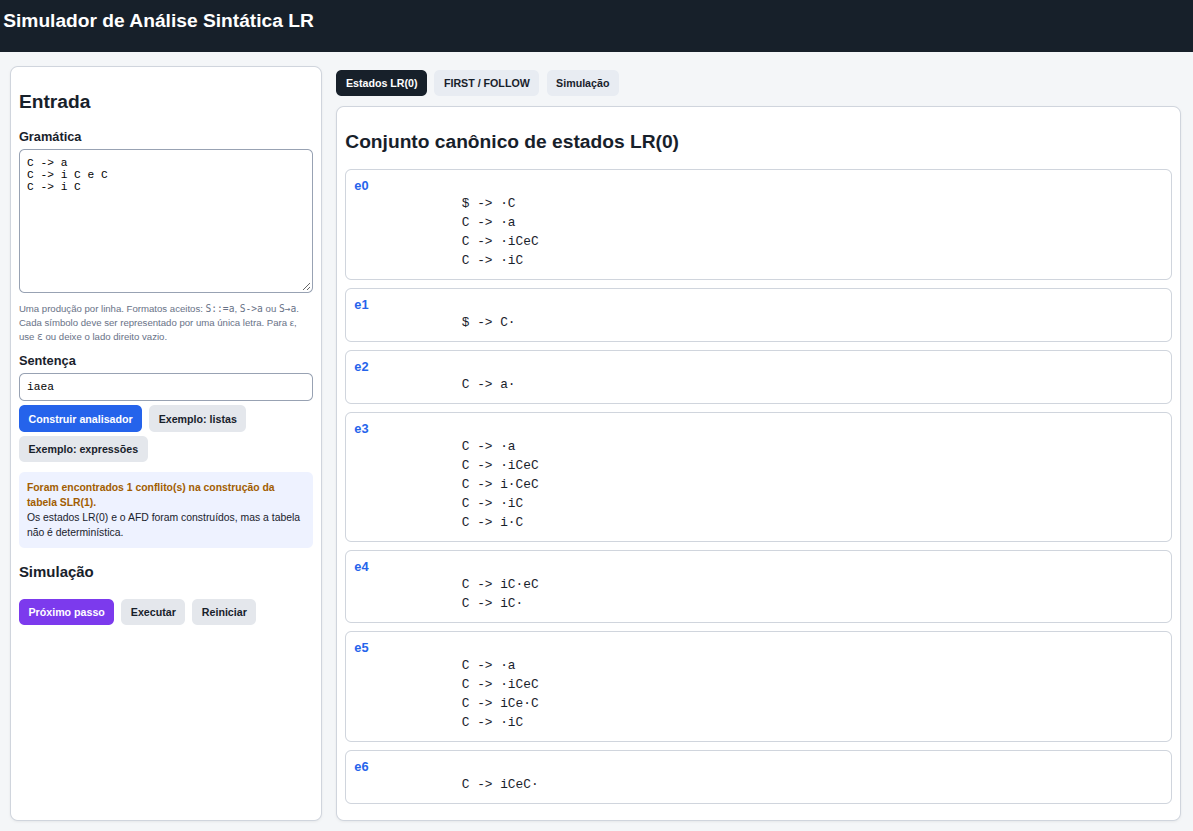
\includegraphics[width=0.6\textwidth]{chapters/images/printscreen/lr.png}}
\caption{Visualização da aplicação interativa}
\end{figure}
\begin{tcolorbox}[enhanced jigsaw, title=Acesso Interativo]
Acesse a simulação em:\par\smallskip
\small\url{https://luizedsilva.github.io/Livro-LTC/p5js/lr/}
\begin{center}
\includegraphics[width=3cm]{chapters/images/qrcode/lr.png}\end{center}
\end{tcolorbox}

A seção deve enfatizar que os conflitos são problemas relacionados à
construção das ações do analisador sintático, e não simplesmente à
execução de operações na pilha. Também é importante distinguir três
conceitos: ambiguidade da gramática, conflito na tabela de análise e
resolução de conflitos por meio de precedência e associatividade.

Há ainda um ajuste conceitual importante no exemplo original: a
gramática apresentada para expressões é ambígua, mas nem todo conflito
de análise LR implica necessariamente uma gramática ambígua. Uma
gramática não ambígua também pode apresentar conflitos para uma
determinada classe de analisadores LR, como LR(0) ou SLR(1).

Abaixo está uma versão revisada, mantendo a sequência didática e a
notação utilizada no capítulo, mas aprofundando a discussão dos dois
tipos de conflito e o papel do Yacc/Bison.

\section{Yacc/Bison -- Geradores de Analisadores
Sintáticos}\label{yaccbison-geradores-de-analisadores-sintuxe1ticos}

Ferramentas como \textbf{Yacc} (\emph{Yet Another Compiler Compiler}) e
\textbf{Bison} são geradores de analisadores sintáticos. A partir de uma
especificação gramatical, essas ferramentas constroem automaticamente um
analisador, normalmente baseado em técnicas de análise sintática
ascendente da família LR.

As gramáticas utilizadas por essas ferramentas são especificadas por
meio de uma notação semelhante à \textbf{Forma de Backus-Naur (BNF)}. A
BNF foi desenvolvida por John Backus e Peter Naur e utilizada
originalmente para a descrição da sintaxe da linguagem ALGOL 60. Por sua
simplicidade e capacidade de representar estruturas hierárquicas, a BNF
e suas variantes tornaram-se amplamente utilizadas na especificação da
sintaxe de linguagens de programação.

Como apresentado anteriormente, as gramáticas livres de contexto
permitem descrever as construções sintáticas de uma linguagem, enquanto
os algoritmos LL e LR estabelecem estratégias para reconhecer essas
construções. No caso do Yacc e do Bison, a especificação gramatical é
utilizada para gerar um analisador sintático ascendente, que realiza
operações de deslocamento e redução (\emph{shift-reduce parsing}).

Entretanto, nem toda gramática livre de contexto pode ser utilizada
diretamente por um gerador de analisadores sintáticos sem dificuldades.
Durante a construção da tabela de análise, podem surgir situações em que
mais de uma ação é possível para um mesmo estado do analisador e um
mesmo símbolo de entrada. Essas situações são denominadas
\textbf{conflitos de análise sintática} e constituem um dos aspectos
importantes no desenvolvimento de gramáticas para compiladores.

\subsection{Exemplo de uma gramática para
expressões}\label{exemplo-de-uma-gramuxe1tica-para-expressuxf5es}

Considere a seguinte gramática para expressões formadas por
identificadores e pelos operadores de adição e multiplicação:

\[
\begin{array}{rccl}\
(1) & E & \rightarrow & E + E \\\
(2) & E & \rightarrow & E * E \\\
(3) & E & \rightarrow & id\
\end{array}
\]

A gramática possui três regras de produção. O símbolo (E) é um
\textbf{não terminal} e representa uma expressão. Já o símbolo (id) é um
\textbf{terminal}, normalmente correspondente a um token produzido pelo
analisador léxico. Os terminais representam os elementos efetivamente
presentes na cadeia de entrada, enquanto os não terminais são utilizados
para representar estruturas sintáticas.

A partir dessa gramática, podemos gerar, por exemplo, a expressão
(x+y*z). Uma possível derivação é:

\[
\begin{array}{rcll}\
E &\Rightarrow & E * E & (r2)\\\
&\Rightarrow & E * z & (r3)\\\
&\Rightarrow & E + E * z & (r1)\\\
&\Rightarrow & E + y * z & (r3)\\\
&\Rightarrow & x + y * z & (r3)\
\end{array}
\]

Em cada passo da derivação, um não terminal é substituído pelo lado
direito de uma de suas produções. O número indicado entre parênteses
identifica a regra de produção utilizada. A derivação começa com o
símbolo inicial (E) e termina quando todos os não terminais foram
substituídos por símbolos terminais.

\subsection{Análise sintática ascendente e operações do
analisador}\label{anuxe1lise-sintuxe1tica-ascendente-e-operauxe7uxf5es-do-analisador}

Na análise sintática ascendente, o processo ocorre na direção inversa.
Em vez de iniciar pelo símbolo inicial e gerar a cadeia de entrada,
parte-se da própria cadeia e procura-se reconstruir o símbolo inicial
por meio de sucessivas \textbf{reduções}. Por esse motivo, esse tipo de
análise também é denominado análise por redução e deslocamento
(\emph{shift-reduce parsing}) ou simplesmente análise \emph{bottom-up}.

O analisador ascendente examina a cadeia de entrada da esquerda para a
direita e utiliza uma pilha para armazenar os símbolos que já foram
processados. Durante a análise, duas operações fundamentais são
realizadas:

\begin{itemize}
\tightlist
\item
  \textbf{Deslocamento (\emph{shift}):} o próximo símbolo da entrada é
  deslocado para a pilha.
\item
  \textbf{Redução (\emph{reduce}):} uma sequência de símbolos no topo da
  pilha que corresponde ao lado direito de uma produção é substituída
  pelo não terminal que aparece no lado esquerdo dessa produção.
\end{itemize}

Assim, uma redução representa a aplicação de uma produção no sentido
inverso. Se a produção é:

\[
A \rightarrow \alpha
\]

a análise ascendente procura uma ocorrência de \(\alpha\) e a substitui
por \(A\).

Por exemplo, considerando a produção:

\[
E \rightarrow id
\]

quando o token \(id\) estiver no topo da pilha e a ação de redução for
selecionada, ele será substituído pelo não terminal \(E\).

A sequência de símbolos que pode ser reduzida em determinado momento é
denominada \textbf{redutendo} (\emph{handle}). Em uma implementação
baseada em pilha, a redução consiste em desempilhar os símbolos que
correspondem ao lado direito da produção e, em seguida, empilhar o não
terminal correspondente ao lado esquerdo.

Para determinar qual operação deve ser executada, o analisador LR
utiliza o estado atual e o próximo símbolo da entrada, denominado
símbolo de antecipação (\emph{lookahead}). Essas informações são
consultadas na tabela de análise sintática, que contém as ações
possíveis para cada situação.

As ações normalmente disponíveis são:

\begin{itemize}
\tightlist
\item
  \texttt{shift}: deslocar o próximo símbolo para a pilha e realizar a
  transição para outro estado;
\item
  \texttt{reduce}: aplicar uma produção da gramática;
\item
  \texttt{accept}: indicar que a cadeia foi reconhecida;
\item
  \texttt{error}: indicar que foi encontrada uma situação sintática
  inválida.
\end{itemize}

É justamente durante a construção dessa tabela que podem surgir
conflitos.

\subsection{Conflitos na análise
sintática}\label{conflitos-na-anuxe1lise-sintuxe1tica}

Um conflito ocorre quando, para uma determinada combinação de estado do
analisador e símbolo de antecipação, existem duas ou mais ações
possíveis. Em outras palavras, o gerador não consegue determinar uma
única ação com base nas informações fornecidas pela gramática e pelo
método de análise utilizado.

Existem dois tipos principais de conflitos:

\begin{itemize}
\tightlist
\item
  \textbf{Conflito deslocamento-redução (\emph{shift-reduce conflict}):}
  ocorre quando o analisador pode escolher entre deslocar o próximo
  símbolo da entrada ou realizar uma redução.
\item
  \textbf{Conflito redução-redução (\emph{reduce-reduce conflict}):}
  ocorre quando duas ou mais produções podem ser utilizadas para
  realizar uma redução na mesma situação.
\end{itemize}

Esses conflitos podem estar relacionados à ambiguidade da gramática, à
insuficiência de informações utilizadas pelo método de análise ou à
forma como as produções foram especificadas.

\subsubsection{\texorpdfstring{Conflito deslocamento-redução
(\emph{shift-reduce
conflict})}{Conflito deslocamento-redução (shift-reduce conflict)}}\label{conflito-deslocamento-reduuxe7uxe3o-shift-reduce-conflict}

Considere novamente a gramática:

\[
\begin{array}{rcl}\
E &\rightarrow& E+E\\\
E &\rightarrow& E*E\\\
E &\rightarrow& id\
\end{array}
\]

Suponha que, durante a análise da expressão \(x+y*z\), o analisador
tenha reconhecido a sequência \(E+E\) e encontre o símbolo \(*\) como
próximo símbolo da entrada.

Nesse momento, existem duas possibilidades:

\begin{enumerate}
\def\labelenumi{\arabic{enumi}.}
\tightlist
\item
  \textbf{Reduzir:} aplicar a produção \(E\rightarrow E+E\),
  substituindo a sequência \(E+E\) por \(E\).
\item
  \textbf{Deslocar:} colocar o símbolo \(*\) na pilha, permitindo que a
  expressão continue sendo analisada.
\end{enumerate}

A primeira possibilidade corresponde à interpretação:

\[
(x+y)*z
\]

A segunda permite continuar o reconhecimento da multiplicação,
produzindo a interpretação:

\[
x+(y*z)
\]

Portanto, o analisador encontra duas ações possíveis: reduzir a soma ou
deslocar o operador de multiplicação. Essa situação caracteriza um
conflito deslocamento-redução.

A origem do conflito está relacionada à ausência de informações sobre a
precedência dos operadores na gramática. A gramática apresentada não
estabelece que a multiplicação deve ser realizada antes da adição.
Consequentemente, as duas interpretações são válidas segundo suas regras
de produção.

\textbf{Precedência e associatividade dos operadores}

Para resolver esse tipo de problema, é necessário estabelecer regras que
determinem a ordem de avaliação dos operadores. Duas propriedades são
particularmente importantes:

\begin{itemize}
\tightlist
\item
  \textbf{Precedência:} determina qual operador deve ser aplicado
  primeiro quando diferentes operadores aparecem em uma mesma expressão.
\item
  \textbf{Associatividade:} determina como operadores de mesma
  precedência são agrupados quando aparecem consecutivamente.
\end{itemize}

Por exemplo, na maioria das linguagens de programação, a multiplicação
possui precedência maior que a adição:

\[
x+y*z \equiv x+(y*z)
\]

Por sua vez, a adição normalmente possui associatividade à esquerda:

\[
x-y-z \equiv (x-y)-z
\]

Essas propriedades podem ser incorporadas diretamente à gramática. Uma
alternativa é reescrever as produções, estabelecendo diferentes níveis
para as expressões:

\[
\begin{array}{rcl}\
E &\rightarrow& E+T \mid T\\\
T &\rightarrow& T*F \mid F\\\
F &\rightarrow& (E) \mid id\
\end{array}
\]

Nessa gramática, \(E\) representa expressões de adição, \(T\) representa
termos que podem conter multiplicações e \(F\) representa fatores. A
separação dos níveis estabelece que a multiplicação deve ser reconhecida
antes da adição.

Além disso, a recursividade à esquerda nas produções de \(E\) e \(T\)
estabelece a associatividade à esquerda dos operadores correspondentes.

Outra possibilidade, particularmente conveniente em ferramentas como
Yacc e Bison, consiste em declarar explicitamente a precedência e a
associatividade dos operadores. Para isso, são utilizadas declarações
específicas na seção de definições da gramática.

Considere o seguinte exemplo:

\begin{verbatim}
%left '+'
%left '*'
\end{verbatim}

A declaração \texttt{\%left} estabelece associatividade à esquerda. A
ordem das declarações determina os níveis de precedência: as declarações
posteriores possuem precedência maior. Portanto, nesse exemplo, a
multiplicação possui precedência maior que a adição.

As principais declarações disponíveis são:

\begin{longtable*}[]{|l|l|}
\toprule\noalign{}
Declaração & Significado \\
\midrule\noalign{}
\endhead
\bottomrule\noalign{}
\endlastfoot
\texttt{\%left} & Associatividade à esquerda \\
\midrule
\texttt{\%right} & Associatividade à direita \\
\midrule
\texttt{\%nonassoc} & Operadores não associativos \\
\midrule
\texttt{\%precedence} & Define precedência sem estabelecer
associatividade \\
\end{longtable*}

Por exemplo, para os operadores aritméticos convencionais, podemos
utilizar:

\begin{verbatim}
%left '+' '-'
%left '*' '/'
%right UMINUS
\end{verbatim}

Nesse caso, adição e subtração possuem o mesmo nível de precedência,
assim como multiplicação e divisão. A multiplicação e a divisão possuem
precedência maior que a adição e a subtração. O identificador
\texttt{UMINUS} representa um nível de precedência utilizado para o
operador de menos unário.

Para associar essa precedência a uma produção específica, pode-se
utilizar a diretiva \texttt{\%prec}:

\begin{verbatim}
expr:
      expr '+' expr
    | expr '*' expr
    | '-' expr %prec UMINUS
    | '(' expr ')'
    | ID
    ;
\end{verbatim}

A diretiva \texttt{\%prec\ UMINUS} determina que a produção
correspondente ao menos unário utilize a precedência declarada para
\texttt{UMINUS}, em vez de utilizar a precedência do símbolo terminal
presente no final da produção.

Dessa maneira, Yacc/Bison podem utilizar as informações de precedência e
associatividade para resolver conflitos deslocamento-redução durante a
construção do analisador.

\textbf{O problema do \texttt{else} pendente}

Outro exemplo clássico de conflito deslocamento-redução ocorre na
construção de comandos condicionais. Considere a seguinte gramática
simplificada:

\[
\begin{array}{rcl}\
S &\rightarrow& \text{if } E \text{ then } S\\\
S &\rightarrow& \text{if } E \text{ then } S \text{ else } S\\\
S &\rightarrow& \text{outro}\
\end{array}
\]

Considere a sequência:

\begin{verbatim}
if E1 then if E2 then S1 else S2
\end{verbatim}

Quando o analisador reconhece \texttt{if\ E1\ then\ if\ E2\ then\ S1} e
encontra o terminal \texttt{else}, pode ocorrer um conflito.

O analisador pode reduzir a construção interna:

\begin{verbatim}
if E2 then S1
\end{verbatim}

ou deslocar o \texttt{else}, associando-o ao comando condicional mais
interno.

Na maioria das linguagens de programação, adota-se a regra segundo a
qual o \texttt{else} está associado ao \texttt{if} mais próximo que
ainda não possui um \texttt{else}. Essa convenção corresponde à escolha
do deslocamento (\emph{shift}) em detrimento da redução (\emph{reduce}).

Esse exemplo demonstra que conflitos deslocamento-redução não estão
restritos a expressões aritméticas. Eles também podem surgir na
especificação de estruturas de controle e outras construções sintáticas.

\subsubsection{\texorpdfstring{Conflito redução-redução
(\emph{reduce-reduce
conflict})}{Conflito redução-redução (reduce-reduce conflict)}}\label{conflito-reduuxe7uxe3o-reduuxe7uxe3o-reduce-reduce-conflict}

O segundo tipo de conflito ocorre quando duas ou mais reduções
diferentes podem ser aplicadas para a mesma situação do analisador.

Considere a seguinte gramática:

\[
\begin{array}{rcl}\
S &\rightarrow& A\\\
S &\rightarrow& B\\\
A &\rightarrow& id\\\
B &\rightarrow& id\
\end{array}
\]

Quando o analisador reconhece o token (id), existem duas possibilidades
de redução:

\[
A\rightarrow id
\]

ou

\[
B\rightarrow id
\]

Ambas as produções possuem o mesmo lado direito, mas produzem não
terminais diferentes. Portanto, o analisador não consegue determinar
qual redução deve ser realizada.

Essa situação caracteriza um conflito redução-redução.

Diferentemente do conflito deslocamento-redução, no qual a escolha
ocorre entre uma redução e um deslocamento, aqui o analisador precisa
escolher entre duas ou mais reduções distintas.

A ocorrência desse conflito geralmente indica um problema na
especificação da gramática. Pode haver produções redundantes,
sobreposição entre estruturas sintáticas ou ausência de informações
suficientes para distinguir as construções.

Uma possível solução consiste em revisar a gramática, eliminando
produções desnecessárias ou reorganizando sua estrutura para que cada
situação de análise determine uma única redução.

Por exemplo, se (A) e (B) representam apenas duas formas de descrever a
mesma construção, pode-se simplificar a gramática:

\[
\begin{array}{rcl}\
S &\rightarrow& id\
\end{array}
\]

É importante destacar que a simples escolha de uma das reduções não
significa que o problema tenha sido resolvido conceitualmente. Em uma
linguagem de programação, diferentes reduções podem corresponder a
diferentes interpretações semânticas, e escolher arbitrariamente uma
delas pode resultar em um analisador que reconhece construções
diferentes daquelas pretendidas.

\subsection{Tratamento de conflitos no
Yacc/Bison}\label{tratamento-de-conflitos-no-yaccbison}

Durante a geração do analisador sintático, Yacc e Bison examinam as
produções da gramática e constroem as estruturas necessárias para a
análise. Quando encontram situações em que mais de uma ação pode ser
executada, identificam e reportam os conflitos.

Na ausência de declarações específicas, o Yacc/Bison utiliza regras de
desempate predefinidas:

\begin{itemize}
\tightlist
\item
  \textbf{Conflito deslocamento-redução:} a ferramenta tradicionalmente
  privilegia o deslocamento (\emph{shift}) em relação à redução
  (\emph{reduce}).
\item
  \textbf{Conflito redução-redução:} a ferramenta privilegia a redução
  correspondente à produção que aparece primeiro na especificação
  gramatical.
\end{itemize}

Essas regras permitem que o analisador seja gerado mesmo quando existem
conflitos. Entretanto, não significam que a gramática esteja
necessariamente correta ou que o comportamento produzido corresponda à
intenção do projetista.

No caso dos conflitos deslocamento-redução, as declarações de
precedência e associatividade podem fornecer informações suficientes
para determinar a ação adequada. Já os conflitos redução-redução
normalmente exigem uma revisão mais cuidadosa da gramática.

O Bison também permite solicitar informações adicionais durante a
geração do analisador, facilitando a identificação das situações
problemáticas. Por exemplo:

\begin{verbatim}
bison -v -d parser.y
\end{verbatim}

A opção \texttt{-v} solicita a geração de um relatório contendo os
estados do analisador e as ações associadas. Esse relatório permite
examinar as situações em que ocorreram conflitos, identificando os
estados e as produções envolvidos. A opção \texttt{-d} solicita a
geração do arquivo de cabeçalho com as definições dos tokens.

O Bison também pode apresentar mensagens mais detalhadas sobre os
conflitos com opções adicionais, como:

\begin{verbatim}
bison -Wcounterexamples parser.y
\end{verbatim}

Essa opção solicita a apresentação de exemplos de cadeias que demonstram
os conflitos encontrados, auxiliando na compreensão e na correção da
gramática.

\section{Arquivo de especificação para
Bison}\label{arquivo-de-especificauxe7uxe3o-para-bison}

O \textbf{Bison} é um gerador de analisadores sintáticos que recebe como
entrada um arquivo contendo a especificação de uma gramática livre de
contexto e produz código-fonte em linguagem C ou C++. Esse código
implementa um analisador sintático capaz de reconhecer cadeias
pertencentes à linguagem definida pela gramática.

Além das produções gramaticais, o arquivo de especificação pode conter
declarações de tokens, informações sobre precedência e associatividade
dos operadores, tipos de dados associados aos símbolos gramaticais e
ações semânticas que serão executadas durante as reduções.

Um arquivo de especificação Bison possui três seções principais,
separadas pelo delimitador \texttt{\%\%}:

\begin{Shaded}
\begin{Highlighting}[]
\OperatorTok{\%\{}
    \CommentTok{/* Definicoes e declaracoes em C */}
\OperatorTok{\%\}}

\CommentTok{/* Declaracoes do Bison */}

\OperatorTok{\%\%}

\CommentTok{/* Regras gramaticais e acoes semanticas */}

\OperatorTok{\%\%}

\CommentTok{/* Subrotinas do usuario */}
\end{Highlighting}
\end{Shaded}

Cada uma dessas seções possui uma finalidade específica.

\subsection{1. Seção de definições e
declarações}\label{seuxe7uxe3o-de-definiuxe7uxf5es-e-declarauxe7uxf5es}

A primeira seção contém as declarações necessárias à construção do
analisador sintático. Pode incluir código C, declarações de variáveis
globais, inclusão de bibliotecas e definições de funções auxiliares.

O trecho delimitado por \texttt{\%\{} e \texttt{\%\}} é denominado bloco
de código inicial (\emph{prologue}). Seu conteúdo é copiado para o
código-fonte gerado pelo Bison.

Por exemplo:

\begin{Shaded}
\begin{Highlighting}[]
\OperatorTok{\%\{}
\PreprocessorTok{\#include }\ImportTok{\textless{}stdio.h\textgreater{}}
\PreprocessorTok{\#include }\ImportTok{\textless{}stdlib.h\textgreater{}}

\DataTypeTok{int}\NormalTok{ yylex}\OperatorTok{(}\DataTypeTok{void}\OperatorTok{);}
\DataTypeTok{void}\NormalTok{ yyerror}\OperatorTok{(}\DataTypeTok{const} \DataTypeTok{char} \OperatorTok{*}\NormalTok{s}\OperatorTok{);}
\OperatorTok{\%\}}
\end{Highlighting}
\end{Shaded}

Nesse exemplo, são incluídas as bibliotecas necessárias e declarados os
protótipos das funções utilizadas pelo analisador.

Após o bloco de código inicial, podem ser especificadas declarações
próprias do Bison. Entre as mais importantes estão:

\begin{longtable*}[]{|
  >{\raggedright\arraybackslash}p{(\linewidth - 4\tabcolsep - 3\arrayrulewidth) * \real{0.5000}}|
  >{\raggedright\arraybackslash}p{(\linewidth - 4\tabcolsep - 3\arrayrulewidth) * \real{0.5000}}|}
\toprule\noalign{}
\begin{minipage}[b]{\linewidth}\smallskip
\raggedright
Declaração
\end{minipage} & \begin{minipage}[b]{\linewidth}\raggedright
Finalidade
\end{minipage} \\
\midrule\noalign{}
\endhead
\bottomrule\noalign{}
\endlastfoot
\texttt{\%token} & Declara os tokens utilizados pela gramática. \\
\midrule
\texttt{\%left} & Declara operadores com associatividade à esquerda. \\
\midrule
\texttt{\%right} & Declara operadores com associatividade à direita. \\
\midrule
\texttt{\%nonassoc} & Declara operadores não associativos. \\
\midrule
\texttt{\%precedence} & Define precedência sem especificar
associatividade. \\
\midrule
\texttt{\%start} & Define explicitamente o símbolo inicial da
gramática. \\
\midrule
\texttt{\%type} & Associa um tipo semântico a símbolos não terminais. \\
\midrule
\texttt{\%union} & Declara os tipos de valores semânticos utilizados
pelo analisador. \\
\end{longtable*}

Os tokens representam as unidades léxicas reconhecidas pelo analisador
léxico. Por exemplo, uma linguagem pode possuir tokens para
identificadores, números, operadores aritméticos e palavras reservadas.

Uma declaração poderia ser:

\begin{Shaded}
\begin{Highlighting}[]
\OperatorTok{\%}\NormalTok{token ID NUM IF ELSE}
\OperatorTok{\%}\NormalTok{left }\CharTok{\textquotesingle{}+\textquotesingle{}} \CharTok{\textquotesingle{}{-}\textquotesingle{}}
\OperatorTok{\%}\NormalTok{left }\CharTok{\textquotesingle{}*\textquotesingle{}} \CharTok{\textquotesingle{}/\textquotesingle{}}
\end{Highlighting}
\end{Shaded}

Nesse caso, são declarados cinco tokens e estabelecidas regras de
precedência e associatividade para os operadores aritméticos.

Quando são utilizados caracteres literais diretamente nas produções,
como \texttt{\textquotesingle{}+\textquotesingle{}},
\texttt{\textquotesingle{}-\textquotesingle{}} e
\texttt{\textquotesingle{}a\textquotesingle{}}, não é necessário
declarar esses caracteres com \texttt{\%token}. O analisador léxico deve
simplesmente retornar o código correspondente ao caractere.

\subsection{2. Seção de regras
gramaticais}\label{seuxe7uxe3o-de-regras-gramaticais}

A segunda seção começa após o primeiro delimitador \texttt{\%\%} e
contém as produções da gramática.

Cada produção possui um símbolo não terminal no lado esquerdo e uma
sequência de símbolos terminais e não terminais no lado direito. As
alternativas de uma mesma produção podem ser escritas separadamente ou
agrupadas utilizando o caractere \texttt{\textbar{}}.

A forma geral é:

\begin{Shaded}
\begin{Highlighting}[]
\NormalTok{nao\_terminal:}
\NormalTok{      alternativa\_1}
\NormalTok{    | alternativa\_2}
\NormalTok{    | alternativa\_3}
\NormalTok{    ;}
\end{Highlighting}
\end{Shaded}

Por exemplo:

\begin{Shaded}
\begin{Highlighting}[]
\NormalTok{expr:}
\NormalTok{      expr \textquotesingle{}+\textquotesingle{} expr}
\NormalTok{    | expr \textquotesingle{}*\textquotesingle{} expr}
\NormalTok{    | ID}
\NormalTok{    ;}
\end{Highlighting}
\end{Shaded}

Essa especificação corresponde à gramática:

\[
\begin{aligned}
E &\rightarrow E+E\\
E &\rightarrow E*E\\
E &\rightarrow id
\end{aligned}
\]

O ponto e vírgula indica o término das alternativas de uma produção.
Portanto, não é necessário escrever uma produção completa em cada linha.

\textbf{Ações semânticas}

Uma característica importante do Bison é a possibilidade de associar
ações semânticas às produções. Essas ações são trechos de código C ou
C++ delimitados por chaves e executados quando o analisador realiza a
redução correspondente.

Por exemplo:

\begin{Shaded}
\begin{Highlighting}[]
\NormalTok{expr:}
\NormalTok{      expr \textquotesingle{}+\textquotesingle{} expr \{ $$ = $1 + $3; \}}
\NormalTok{    | NUM           \{ $$ = $1; \}}
\NormalTok{    ;}
\end{Highlighting}
\end{Shaded}

Nesse exemplo, a ação associada à primeira produção calcula a soma dos
valores das duas expressões.

O Bison disponibiliza referências especiais para acessar os valores
semânticos dos símbolos envolvidos em uma produção:

\begin{itemize}
\tightlist
\item
  \texttt{\$\$}: representa o valor semântico do símbolo não terminal
  produzido, isto é, do lado esquerdo da produção.
\item
  \texttt{\$1}: representa o valor semântico do primeiro símbolo do lado
  direito.
\item
  \texttt{\$2}: representa o valor semântico do segundo símbolo.
\item
  \texttt{\$3}: representa o valor semântico do terceiro símbolo, e
  assim sucessivamente.
\end{itemize}

Assim, para a produção:

\[
E\rightarrow E+E
\]

a expressão \texttt{\$\$\ =\ \$1\ +\ \$3} atribui ao não terminal
produzido o resultado da soma dos valores dos dois operandos.

Para utilizar valores semânticos, é necessário declarar os tipos
correspondentes. Por exemplo:

\begin{Shaded}
\begin{Highlighting}[]
\KeywordTok{\%union}\NormalTok{ \{}
    \DataTypeTok{int}\NormalTok{ inteiro}\OperatorTok{;}
\NormalTok{\}}

\KeywordTok{\%token} \DataTypeTok{\textless{}inteiro\textgreater{}}\NormalTok{ NUM}
\KeywordTok{\%type} \DataTypeTok{\textless{}inteiro\textgreater{}}\NormalTok{ expr}
\end{Highlighting}
\end{Shaded}

Nesse caso, o token \texttt{NUM} e o não terminal \texttt{expr} possuem
valores semânticos do tipo inteiro.

As ações semânticas são fundamentais na construção de compiladores, pois
permitem realizar operações como avaliação de expressões, construção de
árvores sintáticas, verificação de informações e geração de código
intermediário.

\subsection{3. Seção de subrotinas do
usuário}\label{seuxe7uxe3o-de-subrotinas-do-usuuxe1rio}

A terceira seção começa após o segundo delimitador \texttt{\%\%}. Nela
são incluídas as funções auxiliares necessárias à execução do analisador
sintático.

Entre essas funções, destacam-se:

\begin{itemize}
\tightlist
\item
  \texttt{yylex()}: função do analisador léxico, responsável por
  fornecer os próximos tokens ao analisador sintático.
\item
  \texttt{yyerror()}: função responsável pelo tratamento e pela
  apresentação de mensagens de erro sintático.
\item
  \texttt{main()}: função principal do programa, normalmente responsável
  por chamar \texttt{yyparse()}.
\end{itemize}

Um exemplo simplificado é:

\begin{Shaded}
\begin{Highlighting}[]
\DataTypeTok{int}\NormalTok{ yylex}\OperatorTok{(}\DataTypeTok{void}\OperatorTok{)}
\OperatorTok{\{}
    \DataTypeTok{int}\NormalTok{ c}\OperatorTok{;}

    \ControlFlowTok{do} \OperatorTok{\{}
\NormalTok{        c }\OperatorTok{=}\NormalTok{ getchar}\OperatorTok{();}
    \OperatorTok{\}} \ControlFlowTok{while} \OperatorTok{(}\NormalTok{c }\OperatorTok{==} \CharTok{\textquotesingle{} \textquotesingle{}} \OperatorTok{||}\NormalTok{ c }\OperatorTok{==} \CharTok{\textquotesingle{}}\SpecialCharTok{\textbackslash{}t}\CharTok{\textquotesingle{}} \OperatorTok{||}\NormalTok{ c }\OperatorTok{==} \CharTok{\textquotesingle{}}\SpecialCharTok{\textbackslash{}n}\CharTok{\textquotesingle{}}\OperatorTok{);}

    \ControlFlowTok{return}\NormalTok{ c}\OperatorTok{;}
\OperatorTok{\}}

\DataTypeTok{void}\NormalTok{ yyerror}\OperatorTok{(}\DataTypeTok{const} \DataTypeTok{char} \OperatorTok{*}\NormalTok{s}\OperatorTok{)}
\OperatorTok{\{}
\NormalTok{    fprintf}\OperatorTok{(}\NormalTok{stderr}\OperatorTok{,} \StringTok{"Erro sintatico: }\SpecialCharTok{\%s\textbackslash{}n}\StringTok{"}\OperatorTok{,}\NormalTok{ s}\OperatorTok{);}
\OperatorTok{\}}

\DataTypeTok{int}\NormalTok{ main}\OperatorTok{(}\DataTypeTok{void}\OperatorTok{)}
\OperatorTok{\{}
    \ControlFlowTok{return}\NormalTok{ yyparse}\OperatorTok{();}
\OperatorTok{\}}
\end{Highlighting}
\end{Shaded}

Nesse exemplo, o analisador léxico lê os caracteres da entrada padrão e
os retorna individualmente ao analisador sintático. Os espaços em branco
são ignorados.

A função \texttt{yyparse()} é gerada automaticamente pelo Bison e
implementa o algoritmo de análise sintática. Durante sua execução,
solicita tokens à função \texttt{yylex()} e consulta as tabelas de
análise construídas a partir da gramática.

É importante observar que o Bison não gera automaticamente um analisador
léxico completo. A função \texttt{yylex()} precisa ser implementada pelo
programador ou gerada por uma ferramenta específica, como o Flex.

\subsection{Exemplo 1 -- Gramática
recursiva}\label{exemplo-1-gramuxe1tica-recursiva}

Considere a seguinte especificação:

\begin{Shaded}
\begin{Highlighting}[]
\KeywordTok{\%start}\NormalTok{ S}

\BaseNTok{\%\%}

\StringTok{S }\NormalTok{: }\CharTok{\textquotesingle{}a\textquotesingle{}}\NormalTok{ S }\CharTok{\textquotesingle{}c\textquotesingle{}}
\NormalTok{  | }\CharTok{\textquotesingle{}b\textquotesingle{}}
\NormalTok{  ;}

\BaseNTok{\%\%}
\end{Highlighting}
\end{Shaded}

A gramática correspondente é:

\[
S\rightarrow aSc \mid b
\]

A primeira produção é recursiva, pois o não terminal (S) aparece
novamente no lado direito. A segunda produção estabelece a condição de
término da recursão.

A linguagem gerada por essa gramática é:

\[
L(G)=\{a^n b c^n \mid n\geq 0\}
\]

Algumas cadeias pertencentes à linguagem são:

\[
b,\quad abc,\quad aabcc,\quad aaabccc
\]

Por exemplo, a cadeia (aaabccc) pode ser gerada pela seguinte derivação:

\[
\begin{aligned}
S &\Rightarrow aSc\\
  &\Rightarrow aaScc\\
  &\Rightarrow aaaSccc\\
  &\Rightarrow aaabccc
\end{aligned}
\]

O exemplo ilustra como uma gramática recursiva pode ser especificada no
Bison e utilizada para reconhecer uma linguagem formal.

Como a gramática não apresenta ambiguidades nem conflitos para a análise
LR utilizada pelo Bison, o analisador pode ser gerado sem conflitos.

\subsection{Exemplo 2 -- Gramática ambígua e conflito
deslocamento-redução}\label{exemplo-2-gramuxe1tica-ambuxedgua-e-conflito-deslocamento-reduuxe7uxe3o}

Considere agora a seguinte gramática:

\begin{Shaded}
\begin{Highlighting}[]
\BaseNTok{\%\%}

\StringTok{E }\NormalTok{: E }\CharTok{\textquotesingle{}{-}\textquotesingle{}}\NormalTok{ E}
\NormalTok{  | }\CharTok{\textquotesingle{}n\textquotesingle{}}
\NormalTok{  ;}

\BaseNTok{\%\%}
\end{Highlighting}
\end{Shaded}

A gramática corresponde às produções:

\[
\begin{aligned}
E &\rightarrow E-E\\
E &\rightarrow n
\end{aligned}
\]

O terminal \texttt{\textquotesingle{}n\textquotesingle{}} representa um
operando, enquanto o terminal
\texttt{\textquotesingle{}-\textquotesingle{}} representa o operador de
subtração.

Essa gramática permite construir expressões como:

\[
n-n-n
\]

Entretanto, não estabelece a associatividade do operador de subtração.

A expressão pode ser interpretada de duas maneiras:

\[
(n-n)-n
\]

ou:

\[
n-(n-n)
\]

As duas interpretações correspondem a árvores sintáticas diferentes.
Portanto, a gramática é ambígua.

Durante a construção do analisador, o Bison identifica um conflito
deslocamento-redução. Esse conflito ocorre quando o analisador reconhece
uma expressão \(E-E\) e encontra outro símbolo
\texttt{\textquotesingle{}-\textquotesingle{}} na entrada.

Nesse momento, existem duas possibilidades:

\begin{itemize}
\tightlist
\item
  Reduzir \(E-E\) para \(E\), formando uma expressão associativa à
  esquerda.
\item
  Deslocar o próximo operador
  \texttt{\textquotesingle{}-\textquotesingle{}}, permitindo que ele
  seja incorporado à expressão antes da redução.
\end{itemize}

O Bison, na ausência de declarações adicionais, resolve esse conflito
privilegiando o deslocamento. Consequentemente, a interpretação padrão
resultante é associativa à direita:

\[
n-(n-n)
\]

É importante destacar que essa escolha não elimina a ambiguidade da
gramática. Apenas estabelece qual das alternativas será adotada pelo
analisador gerado.

Durante a geração, o Bison apresenta uma mensagem semelhante a:

\begin{Shaded}
\begin{Highlighting}[]
\NormalTok{warning: 1 shift/reduce conflict [{-}Wconflicts{-}sr]}
\end{Highlighting}
\end{Shaded}

A mensagem informa que foi identificado um conflito entre deslocamento e
redução.

\subsection{Exemplo 3 -- Resolução do conflito por
associatividade}\label{exemplo-3-resoluuxe7uxe3o-do-conflito-por-associatividade}

O conflito do exemplo anterior pode ser resolvido declarando
explicitamente a associatividade do operador de subtração.

Considere:

\begin{Shaded}
\begin{Highlighting}[]
\KeywordTok{\%left} \CharTok{\textquotesingle{}{-}\textquotesingle{}}

\BaseNTok{\%\%}

\StringTok{E }\NormalTok{: E }\CharTok{\textquotesingle{}{-}\textquotesingle{}}\NormalTok{ E}
\NormalTok{  | }\CharTok{\textquotesingle{}a\textquotesingle{}}
\NormalTok{  ;}

\BaseNTok{\%\%}
\end{Highlighting}
\end{Shaded}

A declaração:

\begin{Shaded}
\begin{Highlighting}[]
\KeywordTok{\%left} \CharTok{\textquotesingle{}{-}\textquotesingle{}}
\end{Highlighting}
\end{Shaded}

estabelece que o operador de subtração possui associatividade à
esquerda.

Assim, quando o analisador encontra uma situação em que pode deslocar
outro operador ou reduzir uma expressão já reconhecida, a informação de
associatividade permite selecionar a redução.

A expressão:

\[
a-a-a
\]

passa a ser interpretada como:

\[
(a-a)-a
\]

Dessa forma, o Bison consegue resolver o conflito deslocamento-redução
durante a construção do analisador.

Diferentemente do exemplo anterior, a geração não deverá apresentar
conflito deslocamento-redução para essa gramática, pois a declaração de
associatividade fornece a informação necessária para determinar a ação.

É importante observar que a declaração \texttt{\%left} não altera as
produções da gramática. Ela fornece informações adicionais ao gerador
para que este possa resolver determinadas situações de conflito.

\subsection{Os parâmetros do Bison}\label{os-paruxe2metros-do-bison}

Por padrão, o Bison gera um arquivo C com a implementação do analisador
sintático. Entretanto, durante o desenvolvimento de compiladores, é
interessante solicitar também a geração de arquivos auxiliares que
permitam examinar a estrutura do analisador e identificar eventuais
conflitos.

As opções mais utilizadas são:

\begin{longtable*}[]{|
  >{\raggedright\arraybackslash}p{(\linewidth - 4\tabcolsep - 3\arrayrulewidth) * \real{0.5000}}|
  >{\raggedright\arraybackslash}p{(\linewidth - 4\tabcolsep - 3\arrayrulewidth) * \real{0.5000}}|}
\toprule\noalign{}
\begin{minipage}[b]{\linewidth}\smallskip
\raggedright
Opção
\end{minipage} & \begin{minipage}[b]{\linewidth}\raggedright
Finalidade
\end{minipage} \\
\midrule\noalign{}
\endhead
\bottomrule\noalign{}
\endlastfoot
\texttt{-d} & Gera um arquivo de cabeçalho (\texttt{.h}) com as
definições dos tokens. \\
\midrule
\texttt{-v} & Gera um relatório com os estados e as ações do
analisador. \\
\midrule
\texttt{-Wcounterexamples} & Solicita exemplos de cadeias que demonstram
os conflitos encontrados. \\
\midrule
\texttt{-Wall} & Habilita um conjunto de avisos adicionais. \\
\midrule
\texttt{-\/-graph=arquivo.dot} & Gera uma representação do autômato LR
no formato Graphviz. \\
\midrule
\texttt{-\/-report=all} & Solicita informações detalhadas sobre a
construção do analisador. \\
\end{longtable*}

Um comando que reúne essas opções é:

\begin{verbatim}
bison -Wall -Wcounterexamples \
      --report=all \
      --report-file=exemplo.output \
      --graph=exemplo.dot \
      -d \
      -o exemplo.tab.c \
      exemplo.y
\end{verbatim}

Esse comando produz os seguintes arquivos:

\begin{longtable*}[]{|
  >{\raggedright\arraybackslash}p{(\linewidth - 4\tabcolsep - 3\arrayrulewidth) * \real{0.5000}}|
  >{\raggedright\arraybackslash}p{(\linewidth - 4\tabcolsep - 3\arrayrulewidth) * \real{0.5000}}|}
\toprule\noalign{}
\begin{minipage}[b]{\linewidth}\smallskip
\raggedright
Arquivo
\end{minipage} & \begin{minipage}[b]{\linewidth}\raggedright
Conteúdo
\end{minipage} \\
\midrule\noalign{}
\endhead
\bottomrule\noalign{}
\endlastfoot
\texttt{exemplo.tab.c} & Código-fonte C do analisador sintático. \\
\midrule
\texttt{exemplo.tab.h} & Definições dos tokens e outras declarações
públicas do analisador. \\
\midrule
\texttt{exemplo.output} & Relatório detalhado dos estados, transições e
ações da análise sintática. \\
\midrule
\texttt{exemplo.dot} & Representação do autômato LR no formato
Graphviz. \\
\end{longtable*}

O arquivo exemplo.tab.c contém a implementação da função yyparse(),
responsável pela análise sintática. O arquivo de cabeçalho é
particularmente útil quando o analisador léxico está implementado
separadamente, pois permite compartilhar as definições dos tokens.

\textbf{Compilação do analisador}

Para o exemplo:

\begin{Shaded}
\begin{Highlighting}[]
\CommentTok{// Exemplo completo}

\BaseNTok{\%\{}
\PreprocessorTok{\#include }\ImportTok{\textless{}stdio.h\textgreater{}}
\PreprocessorTok{\#include }\ImportTok{\textless{}stdlib.h\textgreater{}}

\DataTypeTok{int}\NormalTok{ yylex}\OperatorTok{(}\DataTypeTok{void}\OperatorTok{);}
\DataTypeTok{void}\NormalTok{ yyerror}\OperatorTok{(}\AttributeTok{const} \DataTypeTok{char} \OperatorTok{*}\NormalTok{s}\OperatorTok{);}
\BaseNTok{\%\}}

\BaseNTok{\%\%}
\CommentTok{// gramatica}
\StringTok{S }\NormalTok{: }\CharTok{\textquotesingle{}a\textquotesingle{}}\NormalTok{ S }\CharTok{\textquotesingle{}c\textquotesingle{}}\NormalTok{;}
\StringTok{S }\NormalTok{: }\CharTok{\textquotesingle{}b\textquotesingle{}}\NormalTok{;}

\BaseNTok{\%\%}
\CommentTok{// codigo do usuario}
\DataTypeTok{int}\NormalTok{ yylex}\OperatorTok{(}\DataTypeTok{void}\OperatorTok{)} \OperatorTok{\{}
    \DataTypeTok{int}\NormalTok{ c}\OperatorTok{;}

    \ControlFlowTok{do} \OperatorTok{\{}
\NormalTok{        c }\OperatorTok{=}\NormalTok{ getchar}\OperatorTok{();}
    \OperatorTok{\}} \ControlFlowTok{while} \OperatorTok{(}\NormalTok{c }\OperatorTok{==} \CharTok{\textquotesingle{} \textquotesingle{}} \OperatorTok{||}\NormalTok{ c }\OperatorTok{==} \CharTok{\textquotesingle{}}\SpecialCharTok{\textbackslash{}t}\CharTok{\textquotesingle{}} \OperatorTok{||}\NormalTok{ c }\OperatorTok{==} \CharTok{\textquotesingle{}}\SpecialCharTok{\textbackslash{}n}\CharTok{\textquotesingle{}}\OperatorTok{);}

    \ControlFlowTok{return}\NormalTok{ c}\OperatorTok{;}
\OperatorTok{\}}

\DataTypeTok{void}\NormalTok{ yyerror}\OperatorTok{(}\AttributeTok{const} \DataTypeTok{char} \OperatorTok{*}\NormalTok{s}\OperatorTok{)} \OperatorTok{\{}
\NormalTok{    fprintf}\OperatorTok{(}\NormalTok{stderr}\OperatorTok{,} \StringTok{"Erro sintatico: }\SpecialCharTok{\%s\textbackslash{}n}\StringTok{"}\OperatorTok{,}\NormalTok{ s}\OperatorTok{);}
\OperatorTok{\}}

\DataTypeTok{int}\NormalTok{ main}\OperatorTok{(}\DataTypeTok{void}\OperatorTok{)} \OperatorTok{\{}
    \ControlFlowTok{return}\NormalTok{ yyparse}\OperatorTok{();}
\OperatorTok{\}}
\end{Highlighting}
\end{Shaded}

Para gerar o analisar (considerando que o código anterior está no
arquivo \texttt{exemplo.y}):

\begin{verbatim}
bison -v -d -g exemplo.y -o exemplo.c
\end{verbatim}

Para produzir um executável, é necessário compilar o código gerado pelo
Bison juntamente com a implementação do analisador léxico e as funções
auxiliares.

Quando essas funções estão no próprio arquivo de especificação, após o
segundo delimitador \%\%, a compilação pode ser realizada diretamente:

\begin{verbatim}
gcc exemplo.c -o exemplo
\end{verbatim}

Depois de compilar o programa, sua execução pode ser realizada
utilizando:

\begin{Shaded}
\begin{Highlighting}[]
\OperatorTok{./}\NormalTok{exemplo}
\end{Highlighting}
\end{Shaded}

O analisador receberá a cadeia pela entrada padrão e verificará se ela
pertence à linguagem definida pela gramática.

\emph{Observação:} quando o analisador léxico é desenvolvido
separadamente, por exemplo, utilizando Flex, a compilação deve incluir
também o código gerado pelo analisador léxico. Nesse caso, é
recomendável utilizar o arquivo de cabeçalho produzido pela opção -d.

Por padrão, o Bison constrói um analisador baseado no método LALR(1).
Durante esse processo, são construídos os estados do autômato e as
tabelas de ações e transições.

\subsection{Visualização gráfica do autômato
LR}\label{visualizauxe7uxe3o-gruxe1fica-do-autuxf4mato-lr}

Além de gerar o código-fonte do analisador, o Bison permite produzir uma
representação gráfica do autômato utilizado na análise sintática.

Essa representação é particularmente útil para compreender como as
produções da gramática são transformadas em estados e transições. Cada
estado do autômato corresponde a um conjunto de itens LR, que
representam produções da gramática em diferentes posições de
reconhecimento.

O autômato é construído a partir das produções e das informações de
análise utilizadas pelo Bison. Suas transições representam os
deslocamentos de símbolos terminais e as transições entre não terminais,
utilizadas no processo de análise.

Para gerar a representação gráfica, utiliza-se a opção:

\begin{Shaded}
\begin{Highlighting}[]
\NormalTok{bison }\OperatorTok{{-}{-}}\NormalTok{graph}\OperatorTok{=}\NormalTok{exemplo}\OperatorTok{.}\NormalTok{dot exemplo}\OperatorTok{.}\NormalTok{y}
\end{Highlighting}
\end{Shaded}

O arquivo exemplo.dot contém a descrição do grafo utilizando a linguagem
DOT, interpretada pela ferramenta Graphviz.

O Graphviz permite transformar essa descrição em diferentes formatos
gráficos, como PNG, SVG e PDF.

Para gerar uma imagem PNG:

\begin{verbatim}
dot -Tpng exemplo.dot -o exemplo.png
\end{verbatim}

Para gerar uma imagem SVG:

\begin{verbatim}
dot -Tsvg exemplo.dot -o exemplo.svg
\end{verbatim}

Também é possível visualizar o arquivo diretamente utilizando o
visualizador interativo xdot:

\begin{verbatim}
xdot exemplo.dot
\end{verbatim}

Caso as ferramentas ainda não estejam instaladas no Ubuntu, podem ser
instaladas por meio de:

\begin{verbatim}
sudo apt install graphviz xdot
\end{verbatim}

\begin{figure}

\centering{

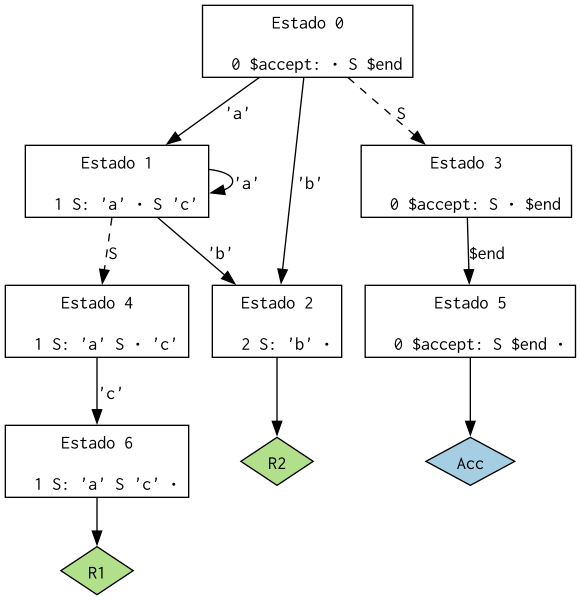
\includegraphics[width=0.6\linewidth,height=\textheight,keepaspectratio]{chapters/images/bison-graph.png}

}

\caption{\label{fig-bison-graph}Representação do autômato gerado}

\end{figure}%

Na representação gráfica do autômato da Figura~\ref{fig-bison-graph}, os
principais elementos são:

\begin{itemize}
\tightlist
\item
  Estados: representados por nós do grafo, contendo os itens LR
  associados a cada estado.
\item
  Transições: representadas por arestas que conectam os estados e
  indicam os símbolos que permitem avançar na análise.
\item
  Estado inicial: representa a configuração inicial do analisador.
\item
  Estados de aceitação: representam situações em que a cadeia pode ser
  reconhecida.
\item
  Itens LR: indicam o ponto em que o analisador se encontra no
  reconhecimento de uma produção.
\end{itemize}

Um item LR pode ser representado, por exemplo, por:

\[
S\rightarrow a\ S\ \bullet\ c
\]

O ponto indica a posição atual do reconhecimento da produção. Nesse
caso, o analisador já reconheceu a sequência \$a~S\$ e espera reconhecer
\(c\) para ter esse item completo.

Já o item:

\[
S\rightarrow a\ S\ c\ \bullet
\]

indica que todos os símbolos do lado direito da produção foram
reconhecidos. Portanto, a produção pode ser candidata a uma redução
\(R1\), neste caso, dependendo do símbolo de antecipação e das ações
definidas na tabela de análise.

\subsection{Visualização dos conflitos no
relatório}\label{visualizauxe7uxe3o-dos-conflitos-no-relatuxf3rio}

Embora o arquivo DOT permita visualizar o autômato, o relatório textual
gerado pela opção -v ou --report é especialmente importante para
examinar os conflitos.

Por exemplo, no segundo exemplo, o relatório pode apresentar uma
situação semelhante a:

\begin{verbatim}
State 4 conflicts: 1 shift/reduce

    1 E: E '-' E •
    1  | E • '-' E

    '-'  shift, and go to state 3

    '-'  [reduce using rule 1 (E)]

    $default  reduce using rule 1 (E)
\end{verbatim}

A representação mostra que, no estado 4, o analisador possui duas
possibilidades para o terminal `-':

\begin{itemize}
\tightlist
\item
  Realizar um deslocamento, avançando para outro estado.
\item
  Realizar uma redução utilizando a produção (E\rightarrow E-E).
\end{itemize}

A existência dessas duas ações para a mesma situação caracteriza o
conflito deslocamento-redução.

No exemplo 3, a declaração \%left `-' permite ao Bison resolver essa
situação. Consequentemente, o relatório não deverá apresentar o conflito
como pendente.

No exemplo 4, por outro lado, a situação envolve o terminal `e'. A
declaração \%left `-' não fornece informações para resolver essa
situação, razão pela qual o conflito permanece.

É importante distinguir o autômato gerado pelo Bison da tabela de
análise sintática. O autômato representa os estados e as transições
utilizados pelo analisador, enquanto a tabela de análise associa os
estados e os símbolos de antecipação às ações de deslocamento, redução,
aceitação ou erro. O relatório textual permite examinar essa relação de
maneira mais detalhada. Relação entre o autômato e os conflitos É
interessante observar que a visualização gráfica permite acompanhar a
construção do autômato que serve de base ao analisador sintático.
Entretanto, a simples observação dos estados e das transições não é
suficiente para compreender todos os conflitos.

Para isso, recomenda-se utilizar conjuntamente os três recursos:

\begin{enumerate}
\def\labelenumi{\arabic{enumi}.}
\tightlist
\item
  Arquivo .dot: permite visualizar graficamente os estados e as
  transições do autômato.
\item
  Arquivo .output: permite examinar os itens LR, os símbolos de
  antecipação e as ações associadas a cada estado.
\item
  Opção -Wcounterexamples: apresenta cadeias que demonstram os conflitos
  e as diferentes possibilidades de análise.
\end{enumerate}

Uma distinção importante para o estudo de compiladores: o autômato
gerado pelo Bison não é o AFD que reconhece diretamente as cadeias da
linguagem. Ele é o autômato de estados LR utilizado na implementação do
analisador sintático.

\textbf{Gerar analisador, relatorio e autômato}

\begin{verbatim}
bison -Wall -Wcounterexamples \
      --report=all \
      --graph=exemplo.dot \
      -d exemplo.y
\end{verbatim}

\textbf{Visualizar o automato}

\begin{verbatim}
xdot exemplo.dot
\end{verbatim}

\textbf{Gerar imagem SVG}

\begin{verbatim}
dot -Tsvg exemplo.dot -o exemplo.svg
\end{verbatim}

\section{Projeto de Compilador - Parte
2}\label{projeto-de-compilador---parte-2}

Na \textbf{Parte 1}, foi implementada uma versão do analisador léxico
responsável por percorrer o programa fonte e identificar os tokens
presentes na entrada. Para algumas classes de tokens, como
\texttt{T\_NUMERO} e \texttt{T\_IDENTIF}, o analisador léxico também
armazena, na variável global \texttt{atomo}, o lexema correspondente ao
token reconhecido. Dessa forma, além de identificar a classe léxica do
elemento encontrado, o analisador mantém a informação necessária para
que esse lexema possa ser utilizada nas etapas posteriores do processo
de compilação.

Nesta \textbf{segunda etapa}, o analisador léxico será integrado ao
analisador sintático, que será gerado automaticamente a partir da
especificação da gramática utilizando a ferramenta \textbf{Bison}. O
objetivo é avançar da identificação isolada dos tokens para o
reconhecimento da estrutura sintática dos programas escritos na
linguagem definida para o projeto.

A linguagem utilizada para a construção do compilador é uma versão
didática denominada \textbf{linguagem \texttt{Simples}}. Essa linguagem
foi especialmente concebida para facilitar o desenvolvimento e a
compreensão de uma primeira versão de um compilador. Por esse motivo,
sua estrutura é deliberadamente reduzida, contendo apenas os elementos
necessários para explorar as principais etapas da construção de um
compilador, desde a análise léxica e sintática até as etapas
posteriores.

A linguagem \texttt{Simples} possui apenas os tipos de dados
\textbf{\texttt{lógico}} e \textbf{\texttt{inteiro}}. As declarações de
variáveis seguem uma sintaxe inspirada em linguagens da família C,
enquanto os comandos disponíveis incluem operações de entrada e saída,
atribuição, seleção e repetição. Entre os comandos definidos pela
linguagem estão \texttt{leia\ VARIAVEL}, para leitura de valores;
\texttt{escreva\ expressão}, para saída de resultados; atribuições
utilizando o operador \texttt{\textless{}-}; além das estruturas
condicionais \texttt{se\ ...\ entao\ ...\ senao\ ...\ fimse} e de
repetição \texttt{enquanto\ ...\ faca\ ...\ fimenquanto}.

Um programa simples escrito nessa linguagem pode ser representado pelo
seguinte exemplo:

\begin{Shaded}
\begin{Highlighting}[]
\NormalTok{programa teste}
\NormalTok{   inteiro A B C }
\NormalTok{inicio}
\NormalTok{   leia A}
\NormalTok{   leia B}
\NormalTok{   se A \textgreater{} B }
\NormalTok{      entao C \textless{}{-} A}
\NormalTok{            A \textless{}{-} B }
\NormalTok{            B \textless{}{-} C }
\NormalTok{      senao }
\NormalTok{   fimse}
\NormalTok{   enquanto A \textless{} B faca}
\NormalTok{      escreva A}
\NormalTok{      A \textless{}{-} A + 1}
\NormalTok{   fimenquanto}
\NormalTok{fimprograma}
\end{Highlighting}
\end{Shaded}

O exemplo apresenta algumas das principais construções disponíveis na
linguagem. Inicialmente, o programa é identificado pelo comando
\texttt{programa}, seguido de seu nome. Em seguida, são declaradas as
variáveis inteiras \texttt{A}, \texttt{B} e \texttt{C}. O bloco iniciado
pela palavra-chave \texttt{inicio} contém os comandos que serão
executados pelo programa.

As instruções \texttt{leia\ A} e \texttt{leia\ B} representam operações
de entrada de dados. Na sequência, a estrutura condicional verifica se o
valor de \texttt{A} é maior que o valor de \texttt{B}. Caso a condição
seja verdadeira, são realizadas três atribuições que utilizam a variável
auxiliar \texttt{C} para trocar os valores de \texttt{A} e \texttt{B}. O
comando \texttt{senao} representa o ramo alternativo da estrutura
condicional, ainda que, neste exemplo, ele não contenha comandos.

Posteriormente, o programa apresenta uma estrutura de repetição definida
pelos comandos \texttt{enquanto\ ...\ faca} e \texttt{fimenquanto}.
Enquanto a condição \texttt{A\ \textless{}\ B} for verdadeira, o valor
de \texttt{A} é apresentado por meio do comando \texttt{escreva} e, em
seguida, incrementado por meio da atribuição
\texttt{A\ \textless{}-\ A\ +\ 1}. Finalmente, o comando
\texttt{fimprograma} delimita o término do programa.

Uma característica importante da linguagem \texttt{Simples} é a ausência
deliberada de alguns elementos de pontuação encontrados normalmente nas
linguagens de programação, como os símbolos \texttt{;} e \texttt{,}.
Essa decisão tem como objetivo tornar a linguagem mais simples para os
primeiros experimentos com a construção de compiladores, reduzindo a
quantidade de elementos sintáticos que precisam ser tratados pelo
analisador léxico e pelo analisador sintático.

Entretanto, essa simplificação também introduz desafios na definição da
gramática. Na ausência de delimitadores explícitos entre determinadas
construções, o analisador sintático pode encontrar situações nas quais
diferentes interpretações da sequência de tokens são possíveis ou nas
quais não é possível determinar claramente onde termina uma construção e
começa outra. Como será discutido nas próximas etapas do desenvolvimento
do compilador, essas características da linguagem \texttt{Simples} terão
impacto direto na construção da gramática e poderão resultar em
conflitos durante a geração do analisador sintático pelo Bison.

Assim, nesta etapa do projeto, o foco passa da identificação individual
dos tokens para a \textbf{análise da sequência de tokens como uma
estrutura sintática}. O analisador léxico desenvolvido na etapa anterior
fornecerá os tokens ao Bison por meio da função \texttt{yylex()},
enquanto o analisador sintático gerado pelo Bison utilizará esses tokens
para verificar se o programa está de acordo com a gramática da linguagem
\texttt{Simples}.

\subsection{Gramática da linguagem
simples}\label{gramuxe1tica-da-linguagem-simples}

Usando a notação apresentada neste livro, a gramática da linguagem
Simples é:

\subsubsection{Estrutura do programa e
declarações}\label{estrutura-do-programa-e-declarauxe7uxf5es}

\[
\begin{aligned}
programa
  &\rightarrow cabecalho \quad variaveis \\
  &\quad T\_INICIO
     \quad lista\_comandos \quad T\_FIM \\
cabecalho
  &\rightarrow T\_PROGRAMA \quad T\_IDENTIF \\
variaveis
  &\rightarrow \lambda \\
  &\mid declaracao\_variaveis \\[3pt]
declaracao\_variaveis
  &\rightarrow tipo \quad lista\_variaveis \quad
                declaracao\_variaveis \\
  &\mid tipo \quad lista\_variaveis \\
tipo
  &\rightarrow T\_LOGICO \\
  &\mid T\_INTEIRO \\
lista\_variaveis
  &\rightarrow T\_IDENTIF \quad lista\_variaveis \\
  &\mid T\_IDENTIF
\end{aligned}
\]

\subsubsection{Lista de comandos e
comandos}\label{lista-de-comandos-e-comandos}

\[
\begin{aligned}
lista\_comandos
  &\rightarrow comando \quad lista\_comandos \\
  &\mid \lambda \\[3pt]
comando
  &\rightarrow entrada\_saida \\
  &\mid repeticao \\
  &\mid selecao \\
  &\mid atribuicao \\[3pt]
entrada\_saida
  &\rightarrow leitura \\
  &\mid escrita \\[3pt]
leitura
  &\rightarrow T\_LEIA \quad T\_IDENTIF \\[3pt]
escrita
  &\rightarrow T\_ESCREVA \quad expressao
\end{aligned}
\]

\subsubsection{Estruturas de controle (repetição, seleção) e
atribuição}\label{estruturas-de-controle-repetiuxe7uxe3o-seleuxe7uxe3o-e-atribuiuxe7uxe3o}

\[
\begin{aligned}
repeticao
  &\rightarrow T\_ENQTO \quad expressao \quad T\_FACA \\
  &\quad lista\_comandos \quad T\_FIMENQTO \\[-1pt]
selecao
  &\rightarrow T\_SE \quad expressao \quad T\_ENTAO \\
  &\quad lista\_comandos \\
  &\quad T\_SENAO \quad lista\_comandos \quad T\_FIMSE \\[-1pt]
atribuicao
  &\rightarrow T\_IDENTIF \quad T\_ATRIB \quad expressao
\end{aligned}
\]

\subsubsection{Expressões}\label{expressuxf5es}

\[
\begin{aligned}
expressao
  &\rightarrow expressao \quad T\_VEZES \quad expressao \\
  &\mid expressao \quad T\_DIV \quad expressao \\
  &\mid expressao \quad T\_MAIS \quad expressao \\
  &\mid expressao \quad T\_MENOS \quad expressao \\
  &\mid expressao \quad T\_MAIOR \quad expressao \\
  &\mid expressao \quad T\_MENOR \quad expressao \\
  &\mid expressao \quad T\_IGUAL \quad expressao \\
  &\mid expressao \quad T\_E \quad expressao \\
  &\mid expressao \quad T\_OU \quad expressao \\
  &\mid termo \\[3pt]
termo
  &\rightarrow T\_IDENTIF \\
  &\mid T\_NUMERO \\
  &\mid T\_V \\
  &\mid T\_F \\
  &\mid T\_NAO \quad termo \\
  &\mid T\_ABRE \quad expressao \quad T\_FECHA
\end{aligned}
\]

Os símbolos não terminais (variáveis da gramática) estão grafados com
letras minúsculas e são: \emph{programa}, \emph{cabecalho},
\emph{variaveis}, \emph{declaracao\_variaveis}, \emph{tipo},
\emph{lista\_variaveis}, \emph{lista\_comandos}, \emph{comando},
\emph{entrada\_saida}, \emph{leitura}, \emph{escrita}, \emph{repeticao},
\emph{condicao}, \emph{atribuicao}, \emph{expressao} e \emph{termo}. O
símbolo de partida é o não-terminal \emph{programa}.

Os símbolos terminais (alfabeto da gramática) estão representados pelas
constantes com o prefixo \texttt{T\_}como: T\_PROGRAMA, T\_INICIO,
T\_FIM, T\_IDENTIF, T\_INTEIRO, T\_LOGICO, T\_LEIA, T\_ESCREVA,
T\_ENQTO, T\_FACA, T\_FIMENQTO, T\_SE, T\_ENTAO, T\_SENAO, T\_FIMSE,
T\_ATRIB, T\_VEZES, T\_DIV, T\_MAIS, T\_MENOS, T\_MAIOR, T\_MENOR,
T\_IGUAL, T\_E, T\_OU, T\_V, T\_F, T\_NAO, T\_ABRE e T\_FECHA. Essas
constantes representam codificações numéricas dos símbolos que são
reconhecidos e retornados pelo analisador léxico.

Para bison, os tokens são definidoss como na listagem seguinte:

\begin{Shaded}
\begin{Highlighting}[]
\OperatorTok{\%}\NormalTok{token T\_PROGRAMA}
\OperatorTok{\%}\NormalTok{token T\_INICIO}
\OperatorTok{\%}\NormalTok{token T\_FIM}
\OperatorTok{\%}\NormalTok{token T\_IDENTIF}
\OperatorTok{\%}\NormalTok{token T\_LEIA}
\OperatorTok{\%}\NormalTok{token T\_ESCREVA}
\OperatorTok{\%}\NormalTok{token T\_ENQTO}
\OperatorTok{...}
\end{Highlighting}
\end{Shaded}

Os códigos utilizados aqui são os mesmos retornados pelo analisador
léxico. Basta incluir o arquivo de cabeçalho que é gerado com a
declaração dessas contantes pela ferramenta bison.

Como pode ser observado, a gramatica de expressões usada na linguagem
Simples é ambígua. Essa ambiguidade é resolvida definindo-se prioridade
entre as operações para a ferramenta Yacc. Fazemos isso com a seguinte
declaração:

\begin{Shaded}
\begin{Highlighting}[]
\OperatorTok{\%}\NormalTok{left T\_E T\_OU}
\OperatorTok{\%}\NormalTok{left T\_IGUAL}
\OperatorTok{\%}\NormalTok{left T\_MAIOR T\_MENOR}
\OperatorTok{\%}\NormalTok{left T\_MAIS T\_MENOS}
\OperatorTok{\%}\NormalTok{left T\_VEZES T\_DIV}
\end{Highlighting}
\end{Shaded}

Com essa declaração, definimos que a multiplicação e a divisão tem
associatividade mais à esquerda e precedência sobre a soma e a
subtração. Soma e subtração tem precedência sobre Operadores relacionais
Maior, Menor e Igual. Os operadores relacionais tem precedência sobre os
operadores lógicos E e OU.

Algumas das regras de produção da gramática SIMPLES, usando a notação de
bison, ficam assim:

\begin{Shaded}
\begin{Highlighting}[]
\NormalTok{programa}
    \OperatorTok{:}\NormalTok{ cabecalho }
\NormalTok{      variaveis }
\NormalTok{      T\_INICIO lista\_comandos T\_FIM}
    \OperatorTok{;}
\NormalTok{cabecalho}
    \OperatorTok{:}\NormalTok{ T\_PROGRAMA T\_IDENTIF}
    \OperatorTok{;}
\NormalTok{variaveis}
    \OperatorTok{:} \CommentTok{/* vazio */}
    \OperatorTok{|}\NormalTok{ declaracao\_variaveis}
    \OperatorTok{;}

\OperatorTok{(...)}

\NormalTok{lista\_comandos}
    \OperatorTok{:} \CommentTok{/* vazio */}
    \OperatorTok{|}\NormalTok{ comando lista\_comandos}
    \OperatorTok{;}

\NormalTok{comando}
    \OperatorTok{:}\NormalTok{ leitura}
    \OperatorTok{|}\NormalTok{ escrita}
    \OperatorTok{|}\NormalTok{ repeticao}
    \OperatorTok{|}\NormalTok{ selecao}
    \OperatorTok{|}\NormalTok{ atribuicao}
    \OperatorTok{;}

\OperatorTok{(...)}

\NormalTok{repeticao}
    \OperatorTok{:}\NormalTok{ T\_ENQTO expressao T\_FACA }
\NormalTok{      lista\_comandos T\_FIMENQTO}
    \OperatorTok{;}

\OperatorTok{(...)}

\NormalTok{expressao}
    \OperatorTok{:}\NormalTok{ expressao T\_VEZES expressao}
    \OperatorTok{|}\NormalTok{ expressao T\_DIV expressao}
    \OperatorTok{|}\NormalTok{ expressao T\_MAIS expressao}
    \OperatorTok{|}\NormalTok{ expressao T\_MENOS expressao}
    \OperatorTok{|}\NormalTok{ expressao T\_MAIOR expressao}
    \OperatorTok{|}\NormalTok{ expressao T\_MENOR expressao}
    \OperatorTok{|}\NormalTok{ expressao T\_IGUAL expressao}
    \OperatorTok{|}\NormalTok{ expressao T\_E expressao}
    \OperatorTok{|}\NormalTok{ expressao T\_OU expressao}
    \OperatorTok{|}\NormalTok{ termo}
    \OperatorTok{;}

\NormalTok{termo}
    \OperatorTok{:}\NormalTok{ T\_IDENTIF}
    \OperatorTok{|}\NormalTok{ T\_NUMERO}
    \OperatorTok{|}\NormalTok{ T\_V}
    \OperatorTok{|}\NormalTok{ T\_F}
    \OperatorTok{|}\NormalTok{ T\_NAO termo}
    \OperatorTok{|}\NormalTok{ T\_ABRE expressao T\_FECHA}
    \OperatorTok{;} 
\end{Highlighting}
\end{Shaded}

\subsubsection{Codigos fontes}\label{codigos-fontes}

O arquivo \texttt{lexico.l} define o \textbf{analisador léxico},
responsável por ler a sequência de caracteres do programa-fonte,
reconhecer os lexemas e convertê-los nos tokens utilizados pelo
analisador sintático. Na seção inicial (\texttt{\%\{\ ...\ \%\}}), é
incluído o arquivo \texttt{sintatico.h}, que contém as definições dos
tokens gerados pelo Bison, além da declaração da função
\texttt{erro\_lexico()}. As expressões regulares \texttt{identificador},
\texttt{numero}, \texttt{espaco} e \texttt{novalinha} definem padrões
para identificadores, números, espaços em branco e quebras de linha.
Entre os delimitadores \texttt{\%\%} são especificadas as regras
léxicas: palavras reservadas, operadores, símbolos lógicos e demais
elementos da linguagem são reconhecidos e associados aos respectivos
tokens, como \texttt{T\_PROG}, \texttt{T\_INICIO} e \texttt{T\_NUMERO};
espaços e quebras de linha são simplesmente ignorados, enquanto
identificadores e números são reconhecidos por meio das expressões
regulares previamente definidas. Qualquer caractere que não corresponda
a uma dessas regras é tratado como \textbf{erro léxico} pela função
\texttt{erro\_lexico()}, que informa o símbolo desconhecido e encerra a
execução. Por fim, a função \texttt{yywrap()} informa ao Flex que não há
mais arquivos de entrada a serem processados.

Código do analisador léxico, adaptado para funcionar integrado com o
sintático:

\begin{Shaded}
\begin{Highlighting}[]
\OperatorTok{\%\{}
\PreprocessorTok{\#include }\ImportTok{"sintatico.h"}
\DataTypeTok{void}\NormalTok{ erro\_lexico}\OperatorTok{(}\DataTypeTok{char} \OperatorTok{*);}
\OperatorTok{\%\}}

\NormalTok{identificador }\OperatorTok{[}\NormalTok{a}\OperatorTok{{-}}\NormalTok{zA}\OperatorTok{{-}}\NormalTok{Z}\OperatorTok{]([}\NormalTok{a}\OperatorTok{{-}}\NormalTok{zA}\OperatorTok{{-}}\NormalTok{Z}\OperatorTok{]|[}\DecValTok{0}\OperatorTok{{-}}\DecValTok{9}\OperatorTok{])*}
\NormalTok{numero }\OperatorTok{[}\DecValTok{0}\OperatorTok{{-}}\DecValTok{9}\OperatorTok{]+}
\NormalTok{espaco }\OperatorTok{[}\NormalTok{ \textbackslash{}t}\OperatorTok{]+}
\NormalTok{novalinha }\OperatorTok{[}\NormalTok{\textbackslash{}n}\OperatorTok{]}

\OperatorTok{\%\%}
\NormalTok{programa          }\OperatorTok{\{} \ControlFlowTok{return}\NormalTok{ T\_PROG}\OperatorTok{;} \OperatorTok{\}}
\NormalTok{inicio            }\OperatorTok{\{} \ControlFlowTok{return}\NormalTok{ T\_INICIO}\OperatorTok{;} \OperatorTok{\}}
\NormalTok{fimprograma       }\OperatorTok{\{} \ControlFlowTok{return}\NormalTok{ T\_FIM}\OperatorTok{;} \OperatorTok{\}}
\NormalTok{leia              }\OperatorTok{\{} \ControlFlowTok{return}\NormalTok{ T\_LEIA}\OperatorTok{;} \OperatorTok{\}}
\NormalTok{escreva           }\OperatorTok{\{} \ControlFlowTok{return}\NormalTok{ T\_ESCREVA}\OperatorTok{;} \OperatorTok{\}}
\NormalTok{se                }\OperatorTok{\{} \ControlFlowTok{return}\NormalTok{ T\_SE}\OperatorTok{;} \OperatorTok{\}}
\NormalTok{entao             }\OperatorTok{\{} \ControlFlowTok{return}\NormalTok{ T\_ENTAO}\OperatorTok{;} \OperatorTok{\}}
\NormalTok{senao             }\OperatorTok{\{} \ControlFlowTok{return}\NormalTok{ T\_SENAO}\OperatorTok{;} \OperatorTok{\}}
\NormalTok{fimse             }\OperatorTok{\{} \ControlFlowTok{return}\NormalTok{ T\_FIMSE}\OperatorTok{;} \OperatorTok{\}}
\NormalTok{enquanto          }\OperatorTok{\{} \ControlFlowTok{return}\NormalTok{ T\_ENQTO}\OperatorTok{;} \OperatorTok{\}}
\NormalTok{faca              }\OperatorTok{\{} \ControlFlowTok{return}\NormalTok{ T\_FACA}\OperatorTok{;} \OperatorTok{\}}
\NormalTok{fimenquanto       }\OperatorTok{\{} \ControlFlowTok{return}\NormalTok{ T\_FIMENQTO}\OperatorTok{;} \OperatorTok{\}}

\NormalTok{inteiro           }\OperatorTok{\{} \ControlFlowTok{return}\NormalTok{ T\_INTEIRO}\OperatorTok{;} \OperatorTok{\}}
\NormalTok{logico            }\OperatorTok{\{} \ControlFlowTok{return}\NormalTok{ T\_LOGICO}\OperatorTok{;} \OperatorTok{\}}

\NormalTok{V                 }\OperatorTok{\{} \ControlFlowTok{return}\NormalTok{ T\_V}\OperatorTok{;} \OperatorTok{\}}
\NormalTok{F                 }\OperatorTok{\{} \ControlFlowTok{return}\NormalTok{ T\_F}\OperatorTok{;} \OperatorTok{\}}

\StringTok{"+"}               \OperatorTok{\{} \ControlFlowTok{return}\NormalTok{ T\_MAIS}\OperatorTok{;} \OperatorTok{\}}
\StringTok{"{-}"}               \OperatorTok{\{} \ControlFlowTok{return}\NormalTok{ T\_MENOS}\OperatorTok{;} \OperatorTok{\}}
\StringTok{"*"}               \OperatorTok{\{} \ControlFlowTok{return}\NormalTok{ T\_VEZES}\OperatorTok{;} \OperatorTok{\}}
\NormalTok{div               }\OperatorTok{\{} \ControlFlowTok{return}\NormalTok{ T\_DIV}\OperatorTok{;} \OperatorTok{\}}
\StringTok{"\textgreater{}"}               \OperatorTok{\{} \ControlFlowTok{return}\NormalTok{ T\_MAIOR}\OperatorTok{;} \OperatorTok{\}}
\StringTok{"\textless{}"}               \OperatorTok{\{} \ControlFlowTok{return}\NormalTok{ T\_MENOR}\OperatorTok{;} \OperatorTok{\}}
\StringTok{"="}               \OperatorTok{\{} \ControlFlowTok{return}\NormalTok{ T\_IGUAL}\OperatorTok{;} \OperatorTok{\}}
\NormalTok{E                 }\OperatorTok{\{} \ControlFlowTok{return}\NormalTok{ T\_E}\OperatorTok{;} \OperatorTok{\}}
\NormalTok{OU                }\OperatorTok{\{} \ControlFlowTok{return}\NormalTok{ T\_OU}\OperatorTok{;} \OperatorTok{\}}
\NormalTok{NAO               }\OperatorTok{\{} \ControlFlowTok{return}\NormalTok{ T\_NAO}\OperatorTok{;} \OperatorTok{\}}
\StringTok{"\textless{}{-}"}              \OperatorTok{\{} \ControlFlowTok{return}\NormalTok{ T\_ATRIB}\OperatorTok{;} \OperatorTok{\}}

\OperatorTok{\{}\NormalTok{identificador}\OperatorTok{\}}   \OperatorTok{\{} \ControlFlowTok{return}\NormalTok{ T\_IDENTIF}\OperatorTok{;} \OperatorTok{\}}
\OperatorTok{\{}\NormalTok{numero}\OperatorTok{\}}          \OperatorTok{\{} \ControlFlowTok{return}\NormalTok{ T\_NUMERO}\OperatorTok{;} \OperatorTok{\}}
\OperatorTok{\{}\NormalTok{espaco}\OperatorTok{\}}          \OperatorTok{\{}  \OperatorTok{\}}
\OperatorTok{\{}\NormalTok{novalinha}\OperatorTok{\}}       \OperatorTok{\{}  \OperatorTok{\}}

\OperatorTok{.}                 \OperatorTok{\{}\NormalTok{ erro\_lexico }\OperatorTok{(}\NormalTok{yytext}\OperatorTok{);} \OperatorTok{\}}
\OperatorTok{\%\%}


\DataTypeTok{void}\NormalTok{ erro\_lexico}\OperatorTok{(}\DataTypeTok{char} \OperatorTok{*}\NormalTok{s}\OperatorTok{)} \OperatorTok{\{}
\NormalTok{    fprintf}\OperatorTok{(}\NormalTok{stderr}\OperatorTok{,} \StringTok{"Erro Léxico.}\SpecialCharTok{\textbackslash{}n}\StringTok{"}\OperatorTok{);}
\NormalTok{    fprintf}\OperatorTok{(}\NormalTok{stderr}\OperatorTok{,} \StringTok{"  símbolo }\SpecialCharTok{\%s}\StringTok{ desconhecido}\SpecialCharTok{\textbackslash{}n\textbackslash{}n}\StringTok{"}\OperatorTok{,}\NormalTok{ s}\OperatorTok{);}
\NormalTok{    exit}\OperatorTok{(}\DecValTok{10}\OperatorTok{);}
\OperatorTok{\}}

\DataTypeTok{int}\NormalTok{ yywrap}\OperatorTok{()} \OperatorTok{\{}
  \ControlFlowTok{return} \DecValTok{1}\OperatorTok{;}
\OperatorTok{\}}
\end{Highlighting}
\end{Shaded}

O arquivo \texttt{sintatico.y} define o \textbf{analisador sintático} da
linguagem, utilizando o Bison para verificar se a sequência de tokens
produzida pelo analisador léxico está de acordo com a gramática da
linguagem. Na seção inicial (\texttt{\%\{\ ...\ \%\}}), são incluídas as
bibliotecas necessárias e declaradas as funções de comunicação com o
analisador léxico, como \texttt{yylex()}, \texttt{yyerror()} e o arquivo
de entrada \texttt{yyin}. As declarações \texttt{\%token} definem os
tokens reconhecidos pelo analisador léxico e utilizados na gramática. A
diretiva \texttt{\%define\ parse.error\ custom} permite personalizar as
mensagens de erro sintático. Entre os delimitadores \texttt{\%\%} é
definida a \textbf{gramática da linguagem}, formada pelas regras para
estrutura do programa, cabeçalho, declaração de variáveis, tipos,
comandos de leitura e escrita, estruturas de repetição e seleção,
atribuições e expressões. Após a gramática, a função \texttt{yyerror()}
trata mensagens gerais de erro do Bison, enquanto a função
\texttt{nome\_token()} associa cada símbolo interno do Bison a uma
descrição em português, permitindo produzir mensagens mais
compreensíveis. A função \texttt{yyreport\_syntax\_error()} utiliza
essas descrições para informar o símbolo encontrado e os símbolos
esperados quando ocorre um erro sintático. Por fim, a função
\texttt{main()} verifica o nome do arquivo fornecido como argumento,
abre o programa-fonte e inicia a análise sintática por meio de
\texttt{yyparse()}, encerrando o processamento após o fechamento do
arquivo.

Código do analisador sintático:

\begin{Shaded}
\begin{Highlighting}[]
\OperatorTok{\%\{}
\PreprocessorTok{\#include }\ImportTok{\textless{}stdio.h\textgreater{}}
\PreprocessorTok{\#include }\ImportTok{\textless{}stdlib.h\textgreater{}}
\PreprocessorTok{\#include }\ImportTok{\textless{}string.h\textgreater{}}

\DataTypeTok{int}\NormalTok{ yylex}\OperatorTok{();}
\DataTypeTok{void}\NormalTok{ yyerror}\OperatorTok{(}\DataTypeTok{const} \DataTypeTok{char} \OperatorTok{*);}
\KeywordTok{extern} \DataTypeTok{FILE} \OperatorTok{*}\NormalTok{yyin}\OperatorTok{;}

\OperatorTok{\%\}}

\OperatorTok{\%}\NormalTok{token T\_PROG}
\OperatorTok{\%}\NormalTok{token T\_INICIO}
\OperatorTok{\%}\NormalTok{token T\_FIM}
\OperatorTok{\%}\NormalTok{token T\_IDENTIF}
\OperatorTok{\%}\NormalTok{token T\_LEIA}
\OperatorTok{\%}\NormalTok{token T\_ESCREVA}
\OperatorTok{\%}\NormalTok{token T\_ENQTO}
\OperatorTok{\%}\NormalTok{token T\_FACA}
\OperatorTok{\%}\NormalTok{token T\_FIMENQTO}
\OperatorTok{\%}\NormalTok{token T\_SE }
\OperatorTok{\%}\NormalTok{token T\_ENTAO}
\OperatorTok{\%}\NormalTok{token T\_SENAO}
\OperatorTok{\%}\NormalTok{token T\_FIMSE}
\OperatorTok{\%}\NormalTok{token T\_ATRIB}
\OperatorTok{\%}\NormalTok{token T\_VEZES}
\OperatorTok{\%}\NormalTok{token T\_DIV}
\OperatorTok{\%}\NormalTok{token T\_MAIS}
\OperatorTok{\%}\NormalTok{token T\_MENOS}
\OperatorTok{\%}\NormalTok{token T\_MAIOR}
\OperatorTok{\%}\NormalTok{token T\_MENOR}
\OperatorTok{\%}\NormalTok{token T\_IGUAL}
\OperatorTok{\%}\NormalTok{token T\_E }
\OperatorTok{\%}\NormalTok{token T\_OU}
\OperatorTok{\%}\NormalTok{token T\_V }
\OperatorTok{\%}\NormalTok{token T\_F }
\OperatorTok{\%}\NormalTok{token T\_NUMERO}
\OperatorTok{\%}\NormalTok{token T\_NAO }
\OperatorTok{\%}\NormalTok{token T\_ABRE}
\OperatorTok{\%}\NormalTok{token T\_FECHA}
\OperatorTok{\%}\NormalTok{token T\_LOGICO}
\OperatorTok{\%}\NormalTok{token T\_INTEIRO}

\OperatorTok{\%}\NormalTok{define parse}\OperatorTok{.}\NormalTok{error custom}

\OperatorTok{\%}\NormalTok{left T\_E T\_OU}
\OperatorTok{\%}\NormalTok{left T\_IGUAL}
\OperatorTok{\%}\NormalTok{left T\_MAIOR T\_MENOR}
\OperatorTok{\%}\NormalTok{left T\_MAIS T\_MENOS}
\OperatorTok{\%}\NormalTok{left T\_VEZES T\_DIV}

\OperatorTok{\%\%}
\NormalTok{programa}
    \OperatorTok{:}\NormalTok{ cabecalho }
\NormalTok{      variaveis }
\NormalTok{      T\_INICIO lista\_comandos T\_FIM}
    \OperatorTok{;}

\NormalTok{cabecalho}
    \OperatorTok{:}\NormalTok{ T\_PROG T\_IDENTIF}
    \OperatorTok{;}

\NormalTok{variaveis}
    \OperatorTok{:} \CommentTok{/* vazio */}
    \OperatorTok{|}\NormalTok{ declaracao\_variaveis}
    \OperatorTok{;}

\NormalTok{declaracao\_variaveis}
    \OperatorTok{:}\NormalTok{ tipo lista\_variaveis declaracao\_variaveis}
    \OperatorTok{|}\NormalTok{ tipo lista\_variaveis}
    \OperatorTok{;}

\NormalTok{tipo}
    \OperatorTok{:}\NormalTok{ T\_LOGICO}
    \OperatorTok{|}\NormalTok{ T\_INTEIRO}
    \OperatorTok{;}

\NormalTok{lista\_variaveis}
    \OperatorTok{:}\NormalTok{ lista\_variaveis T\_IDENTIF}
    \OperatorTok{|}\NormalTok{ T\_IDENTIF}
    \OperatorTok{;}

\NormalTok{lista\_comandos}
    \OperatorTok{:} \CommentTok{/* vazio */}
    \OperatorTok{|}\NormalTok{ comando lista\_comandos}
    \OperatorTok{;}

\NormalTok{comando}
    \OperatorTok{:}\NormalTok{ leitura}
    \OperatorTok{|}\NormalTok{ escrita}
    \OperatorTok{|}\NormalTok{ repeticao}
    \OperatorTok{|}\NormalTok{ selecao}
    \OperatorTok{|}\NormalTok{ atribuicao}
    \OperatorTok{;}

\NormalTok{leitura}
    \OperatorTok{:}\NormalTok{ T\_LEIA T\_IDENTIF}
    \OperatorTok{;}

\NormalTok{escrita}
    \OperatorTok{:}\NormalTok{ T\_ESCREVA expressao}
    \OperatorTok{;}

\NormalTok{repeticao}
    \OperatorTok{:}\NormalTok{ T\_ENQTO expressao T\_FACA }
\NormalTok{      lista\_comandos T\_FIMENQTO}
    \OperatorTok{;}

\NormalTok{selecao}
    \OperatorTok{:}\NormalTok{ T\_SE expressao T\_ENTAO }
\NormalTok{      lista\_comandos T\_SENAO }
\NormalTok{      lista\_comandos T\_FIMSE}
    \OperatorTok{;}

\NormalTok{atribuicao}
    \OperatorTok{:}\NormalTok{ T\_IDENTIF T\_ATRIB expressao}
    \OperatorTok{;}

\NormalTok{expressao}
    \OperatorTok{:}\NormalTok{ expressao T\_VEZES expressao}
    \OperatorTok{|}\NormalTok{ expressao T\_DIV expressao}
    \OperatorTok{|}\NormalTok{ expressao T\_MAIS expressao}
    \OperatorTok{|}\NormalTok{ expressao T\_MENOS expressao}
    \OperatorTok{|}\NormalTok{ expressao T\_MAIOR expressao}
    \OperatorTok{|}\NormalTok{ expressao T\_MENOR expressao}
    \OperatorTok{|}\NormalTok{ expressao T\_IGUAL expressao}
    \OperatorTok{|}\NormalTok{ expressao T\_E expressao}
    \OperatorTok{|}\NormalTok{ expressao T\_OU expressao}
    \OperatorTok{|}\NormalTok{ termo}
    \OperatorTok{;}

\NormalTok{termo}
    \OperatorTok{:}\NormalTok{ T\_IDENTIF}
    \OperatorTok{|}\NormalTok{ T\_NUMERO}
    \OperatorTok{|}\NormalTok{ T\_V}
    \OperatorTok{|}\NormalTok{ T\_F}
    \OperatorTok{|}\NormalTok{ T\_NAO termo}
    \OperatorTok{|}\NormalTok{ T\_ABRE expressao T\_FECHA}
    \OperatorTok{;} 

\OperatorTok{\%\%}

\DataTypeTok{void}\NormalTok{ yyerror}\OperatorTok{(}\DataTypeTok{const} \DataTypeTok{char} \OperatorTok{*}\NormalTok{mensagem}\OperatorTok{)}
\OperatorTok{\{}
\NormalTok{    fprintf}\OperatorTok{(}\NormalTok{stderr}\OperatorTok{,} \StringTok{"Erro Interno: }\SpecialCharTok{\%s\textbackslash{}n}\StringTok{"}\OperatorTok{,}\NormalTok{ mensagem}\OperatorTok{);}
\OperatorTok{\}}

\DataTypeTok{static} \DataTypeTok{const} \DataTypeTok{char} \OperatorTok{*}\NormalTok{nome\_token}\OperatorTok{(}\NormalTok{yysymbol\_kind\_t token}\OperatorTok{)}
\OperatorTok{\{}
    \DataTypeTok{static} \DataTypeTok{const} \DataTypeTok{char} \OperatorTok{*}\NormalTok{nomes}\OperatorTok{[]} \OperatorTok{=} \OperatorTok{\{}
        \OperatorTok{[}\NormalTok{YYSYMBOL\_T\_PROG}\OperatorTok{]}      \OperatorTok{=} \StringTok{"programa"}\OperatorTok{,}
        \OperatorTok{[}\NormalTok{YYSYMBOL\_T\_INICIO}\OperatorTok{]}    \OperatorTok{=} \StringTok{"início"}\OperatorTok{,}
        \OperatorTok{[}\NormalTok{YYSYMBOL\_T\_FIM}\OperatorTok{]}       \OperatorTok{=} \StringTok{"fim"}\OperatorTok{,}
        \OperatorTok{[}\NormalTok{YYSYMBOL\_T\_IDENTIF}\OperatorTok{]}   \OperatorTok{=} \StringTok{"identificador"}\OperatorTok{,}
        \OperatorTok{[}\NormalTok{YYSYMBOL\_T\_LEIA}\OperatorTok{]}      \OperatorTok{=} \StringTok{"leia"}\OperatorTok{,}
        \OperatorTok{[}\NormalTok{YYSYMBOL\_T\_ESCREVA}\OperatorTok{]}   \OperatorTok{=} \StringTok{"escreva"}\OperatorTok{,}
        \OperatorTok{[}\NormalTok{YYSYMBOL\_T\_ENQTO}\OperatorTok{]}     \OperatorTok{=} \StringTok{"enquanto"}\OperatorTok{,}
        \OperatorTok{[}\NormalTok{YYSYMBOL\_T\_FACA}\OperatorTok{]}      \OperatorTok{=} \StringTok{"faça"}\OperatorTok{,}
        \OperatorTok{[}\NormalTok{YYSYMBOL\_T\_FIMENQTO}\OperatorTok{]}  \OperatorTok{=} \StringTok{"fim{-}enquanto"}\OperatorTok{,}
        \OperatorTok{[}\NormalTok{YYSYMBOL\_T\_SE}\OperatorTok{]}        \OperatorTok{=} \StringTok{"se"}\OperatorTok{,}
        \OperatorTok{[}\NormalTok{YYSYMBOL\_T\_ENTAO}\OperatorTok{]}     \OperatorTok{=} \StringTok{"então"}\OperatorTok{,}
        \OperatorTok{[}\NormalTok{YYSYMBOL\_T\_SENAO}\OperatorTok{]}     \OperatorTok{=} \StringTok{"senão"}\OperatorTok{,}
        \OperatorTok{[}\NormalTok{YYSYMBOL\_T\_FIMSE}\OperatorTok{]}     \OperatorTok{=} \StringTok{"fim{-}se"}\OperatorTok{,}
        \OperatorTok{[}\NormalTok{YYSYMBOL\_T\_ATRIB}\OperatorTok{]}     \OperatorTok{=} \StringTok{"atribuição"}\OperatorTok{,}
        \OperatorTok{[}\NormalTok{YYSYMBOL\_T\_VEZES}\OperatorTok{]}     \OperatorTok{=} \StringTok{"\textquotesingle{}*\textquotesingle{}"}\OperatorTok{,}
        \OperatorTok{[}\NormalTok{YYSYMBOL\_T\_DIV}\OperatorTok{]}       \OperatorTok{=} \StringTok{"\textquotesingle{}/\textquotesingle{}"}\OperatorTok{,}
        \OperatorTok{[}\NormalTok{YYSYMBOL\_T\_MAIS}\OperatorTok{]}      \OperatorTok{=} \StringTok{"\textquotesingle{}+\textquotesingle{}"}\OperatorTok{,}
        \OperatorTok{[}\NormalTok{YYSYMBOL\_T\_MENOS}\OperatorTok{]}     \OperatorTok{=} \StringTok{"\textquotesingle{}{-}\textquotesingle{}"}\OperatorTok{,}
        \OperatorTok{[}\NormalTok{YYSYMBOL\_T\_MAIOR}\OperatorTok{]}     \OperatorTok{=} \StringTok{"\textquotesingle{}\textgreater{}\textquotesingle{}"}\OperatorTok{,}
        \OperatorTok{[}\NormalTok{YYSYMBOL\_T\_MENOR}\OperatorTok{]}     \OperatorTok{=} \StringTok{"\textquotesingle{}\textless{}\textquotesingle{}"}\OperatorTok{,}
        \OperatorTok{[}\NormalTok{YYSYMBOL\_T\_IGUAL}\OperatorTok{]}     \OperatorTok{=} \StringTok{"\textquotesingle{}=\textquotesingle{}"}\OperatorTok{,}
        \OperatorTok{[}\NormalTok{YYSYMBOL\_T\_E}\OperatorTok{]}         \OperatorTok{=} \StringTok{"e"}\OperatorTok{,}
        \OperatorTok{[}\NormalTok{YYSYMBOL\_T\_OU}\OperatorTok{]}        \OperatorTok{=} \StringTok{"ou"}\OperatorTok{,}
        \OperatorTok{[}\NormalTok{YYSYMBOL\_T\_V}\OperatorTok{]}         \OperatorTok{=} \StringTok{"verdadeiro"}\OperatorTok{,}
        \OperatorTok{[}\NormalTok{YYSYMBOL\_T\_F}\OperatorTok{]}         \OperatorTok{=} \StringTok{"falso"}\OperatorTok{,}
        \OperatorTok{[}\NormalTok{YYSYMBOL\_T\_NUMERO}\OperatorTok{]}    \OperatorTok{=} \StringTok{"número"}\OperatorTok{,}
        \OperatorTok{[}\NormalTok{YYSYMBOL\_T\_NAO}\OperatorTok{]}       \OperatorTok{=} \StringTok{"não"}\OperatorTok{,}
        \OperatorTok{[}\NormalTok{YYSYMBOL\_T\_ABRE}\OperatorTok{]}      \OperatorTok{=} \StringTok{"\textquotesingle{}(\textquotesingle{}"}\OperatorTok{,}
        \OperatorTok{[}\NormalTok{YYSYMBOL\_T\_FECHA}\OperatorTok{]}     \OperatorTok{=} \StringTok{"\textquotesingle{})\textquotesingle{}"}\OperatorTok{,}
        \OperatorTok{[}\NormalTok{YYSYMBOL\_T\_LOGICO}\OperatorTok{]}    \OperatorTok{=} \StringTok{"lógico"}\OperatorTok{,}
        \OperatorTok{[}\NormalTok{YYSYMBOL\_T\_INTEIRO}\OperatorTok{]}   \OperatorTok{=} \StringTok{"inteiro"}
    \OperatorTok{\};}

    \ControlFlowTok{if} \OperatorTok{(}\NormalTok{token }\OperatorTok{\textgreater{}=} \DecValTok{0} \OperatorTok{\&\&}
\NormalTok{        token }\OperatorTok{\textless{}} \KeywordTok{sizeof}\OperatorTok{(}\NormalTok{nomes}\OperatorTok{)} \OperatorTok{/} \KeywordTok{sizeof}\OperatorTok{(}\NormalTok{nomes}\OperatorTok{[}\DecValTok{0}\OperatorTok{])} \OperatorTok{\&\&}
\NormalTok{        nomes}\OperatorTok{[}\NormalTok{token}\OperatorTok{]} \OperatorTok{!=}\NormalTok{ NULL}\OperatorTok{)}
        \ControlFlowTok{return}\NormalTok{ nomes}\OperatorTok{[}\NormalTok{token}\OperatorTok{];}

    \ControlFlowTok{return} \StringTok{"símbolo desconhecido"}\OperatorTok{;}
\OperatorTok{\}}

\DataTypeTok{static} \DataTypeTok{int}\NormalTok{ yyreport\_syntax\_error}\OperatorTok{(}\DataTypeTok{const}\NormalTok{ yypcontext\_t }\OperatorTok{*}\NormalTok{ctx}\OperatorTok{)}
\OperatorTok{\{}
\NormalTok{    yysymbol\_kind\_t token}\OperatorTok{;}
\NormalTok{    yysymbol\_kind\_t expected}\OperatorTok{[}\DecValTok{10}\OperatorTok{];}

\NormalTok{    token }\OperatorTok{=}\NormalTok{ yypcontext\_token}\OperatorTok{(}\NormalTok{ctx}\OperatorTok{);}

\NormalTok{    fprintf}\OperatorTok{(}\NormalTok{stderr}\OperatorTok{,} \StringTok{"Erro de sintaxe.}\SpecialCharTok{\textbackslash{}n}\StringTok{"}\OperatorTok{);}
\NormalTok{    fprintf}\OperatorTok{(}\NormalTok{stderr}\OperatorTok{,} \StringTok{"  Símbolo encontrado: }\SpecialCharTok{\%s\textbackslash{}n}\StringTok{"}\OperatorTok{,}
\NormalTok{            nome\_token}\OperatorTok{(}\NormalTok{token}\OperatorTok{));}

\NormalTok{    fprintf}\OperatorTok{(}\NormalTok{stderr}\OperatorTok{,} \StringTok{"  Símbolos esperados: "}\OperatorTok{);}

    \DataTypeTok{int}\NormalTok{ n }\OperatorTok{=}\NormalTok{ yypcontext\_expected\_tokens}\OperatorTok{(}\NormalTok{ctx}\OperatorTok{,}\NormalTok{ expected}\OperatorTok{,} \DecValTok{10}\OperatorTok{);}

    \ControlFlowTok{for} \OperatorTok{(}\DataTypeTok{int}\NormalTok{ i }\OperatorTok{=} \DecValTok{0}\OperatorTok{;}\NormalTok{ i }\OperatorTok{\textless{}}\NormalTok{ n}\OperatorTok{;}\NormalTok{ i}\OperatorTok{++)} \OperatorTok{\{}
        \ControlFlowTok{if} \OperatorTok{(}\NormalTok{i }\OperatorTok{\textgreater{}} \DecValTok{0}\OperatorTok{)}
\NormalTok{            fprintf}\OperatorTok{(}\NormalTok{stderr}\OperatorTok{,} \StringTok{", "}\OperatorTok{);}

\NormalTok{        fprintf}\OperatorTok{(}\NormalTok{stderr}\OperatorTok{,} \StringTok{"}\SpecialCharTok{\%s}\StringTok{"}\OperatorTok{,}\NormalTok{ nome\_token}\OperatorTok{(}\NormalTok{expected}\OperatorTok{[}\NormalTok{i}\OperatorTok{]));}
    \OperatorTok{\}}
\NormalTok{    fprintf}\OperatorTok{(}\NormalTok{stderr}\OperatorTok{,} \StringTok{"}\SpecialCharTok{\textbackslash{}n\textbackslash{}n}\StringTok{"}\OperatorTok{);}
    \ControlFlowTok{return} \DecValTok{0}\OperatorTok{;}
\OperatorTok{\}}

\DataTypeTok{int}\NormalTok{ main}\OperatorTok{(}\DataTypeTok{int}\NormalTok{ argc}\OperatorTok{,} \DataTypeTok{char} \OperatorTok{*}\NormalTok{argv}\OperatorTok{[])} \OperatorTok{\{}
    \ControlFlowTok{if} \OperatorTok{(}\NormalTok{argc }\OperatorTok{\textless{}} \DecValTok{2}\OperatorTok{)} \OperatorTok{\{}
\NormalTok{        printf}\OperatorTok{(}\StringTok{"Uso:}\SpecialCharTok{\textbackslash{}n}\StringTok{ }\SpecialCharTok{\textbackslash{}t\%s}\StringTok{ \textless{}nomeprog.simples\textgreater{}}\SpecialCharTok{\textbackslash{}n\textbackslash{}n}\StringTok{"}\OperatorTok{,}\NormalTok{ argv}\OperatorTok{[}\DecValTok{0}\OperatorTok{]);}
\NormalTok{        exit}\OperatorTok{(}\DecValTok{20}\OperatorTok{);}
    \OperatorTok{\}}
\NormalTok{    yyin }\OperatorTok{=}\NormalTok{ fopen}\OperatorTok{(}\NormalTok{argv}\OperatorTok{[}\DecValTok{1}\OperatorTok{],} \StringTok{"rt"}\OperatorTok{);}
\NormalTok{    yyparse}\OperatorTok{();}
\NormalTok{    fclose}\OperatorTok{(}\NormalTok{yyin}\OperatorTok{);}
\OperatorTok{\}}
\end{Highlighting}
\end{Shaded}

O arquivo \texttt{makefile} automatiza o processo de \textbf{geração e
compilação do compilador da linguagem Simples}, evitando a necessidade
de executar manualmente cada comando. O alvo \texttt{simples} estabelece
como dependências os arquivos \texttt{lexico.l} e \texttt{sintatico.y} e
executa, inicialmente, o \textbf{Flex} para transformar as regras
léxicas de \texttt{lexico.l} no código-fonte C \texttt{lexico.c}. Em
seguida, o \textbf{Bison} processa \texttt{sintatico.y}, gerando o
analisador sintático \texttt{sintatico.c}, o arquivo de cabeçalho
\texttt{sintatico.h}, que contém as definições dos tokens utilizados
pelo analisador léxico, e o arquivo \texttt{sintatico.output}, que
apresenta informações sobre a gramática e as tabelas do analisador
gerado. Por fim, o compilador \texttt{gcc} combina \texttt{lexico.c} e
\texttt{sintatico.c} e gera o executável \texttt{simples}. O alvo
\texttt{limpa} remove os arquivos gerados durante o processo de
compilação, permitindo realizar uma nova geração dos arquivos a partir
dos fontes originais.

Código do \texttt{makefile} para automatizar a construção do compilador:

\begin{Shaded}
\begin{Highlighting}[]
\NormalTok{simples}\OperatorTok{:}\NormalTok{ lexico}\OperatorTok{.}\NormalTok{l sintatico}\OperatorTok{.}\NormalTok{y }\OperatorTok{;}\NormalTok{\textbackslash{}}
\NormalTok{    flex }\OperatorTok{{-}}\NormalTok{o lexico}\OperatorTok{.}\NormalTok{c lexico}\OperatorTok{.}\NormalTok{l}
\NormalTok{    bison }\OperatorTok{{-}}\NormalTok{o sintatico}\OperatorTok{.}\NormalTok{c sintatico}\OperatorTok{.}\NormalTok{y }\OperatorTok{{-}}\NormalTok{v }\OperatorTok{{-}}\NormalTok{d}
\NormalTok{    gcc lexico}\OperatorTok{.}\NormalTok{c sintatico}\OperatorTok{.}\NormalTok{c }\OperatorTok{{-}}\NormalTok{o simples}

\NormalTok{limpa}\OperatorTok{:} \OperatorTok{;}\NormalTok{\textbackslash{} }
\NormalTok{    rm simples lexico}\OperatorTok{.}\NormalTok{c sintatico}\OperatorTok{.}\NormalTok{c sintatico}\OperatorTok{.}\NormalTok{h sintatico}\OperatorTok{.}\NormalTok{output simples}
\end{Highlighting}
\end{Shaded}

\subsection{Simulador do Analisador Sintático para Linguagem
Simples}\label{simulador-do-analisador-sintuxe1tico-para-linguagem-simples}

O exemplo interativo a seguir, demonstra o processo de construção da
árvore sintática para um programa. Para o programa fonte digitado, após
clicar no botão `Construir Árvore', são gerados e calculados os tokens e
os nós da árvore sintática. As folhas da árvore estão relacionadas as
informações do código.

\begin{figure}[H]
\centering
\fbox{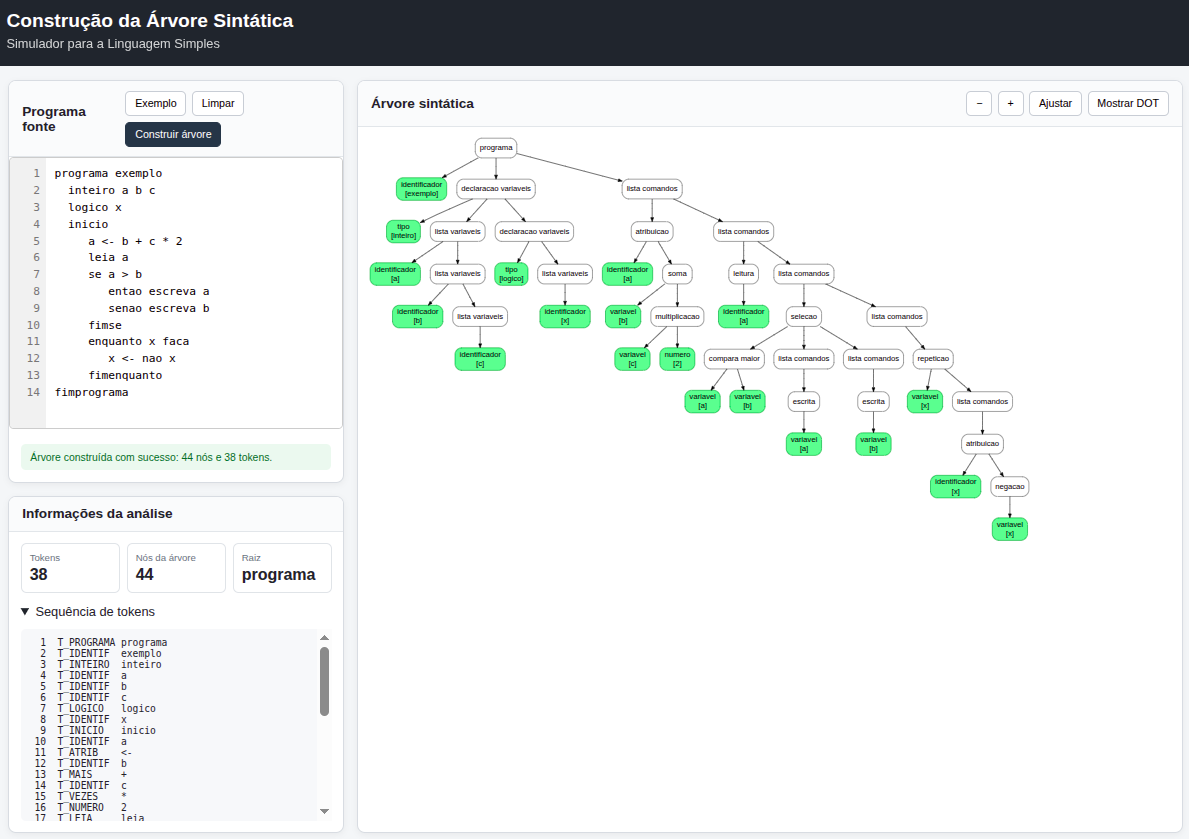
\includegraphics[width=0.6\textwidth]{chapters/images/printscreen/syntaxTree.png}}
\caption{Visualização da aplicação interativa}
\end{figure}
\begin{tcolorbox}[enhanced jigsaw, title=Acesso Interativo]
Acesse a simulação em:\par\smallskip
\small\url{https://luizedsilva.github.io/Livro-LTC/p5js/syntaxTree/}
\begin{center}
\includegraphics[width=3cm]{chapters/images/qrcode/syntaxTree.png}\end{center}
\end{tcolorbox}

\bookmarksetup{startatroot}

\chapter{A Máquina de Turing e as Máquinas
Virtuais}\label{a-muxe1quina-de-turing-e-as-muxe1quinas-virtuais}

\begin{center}
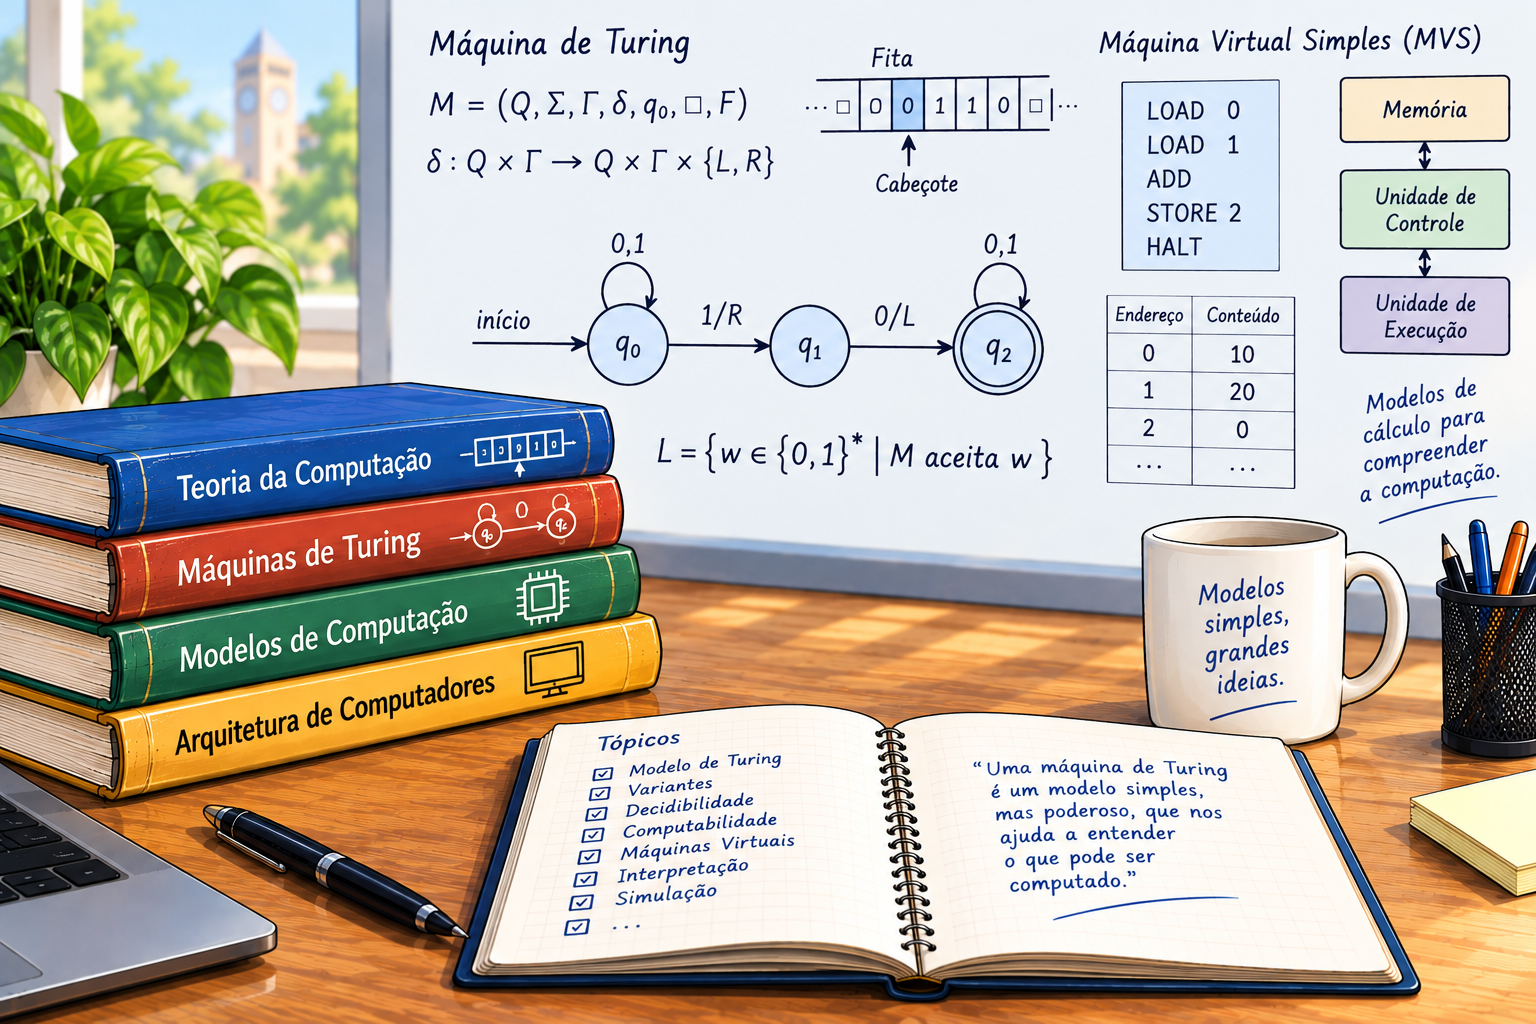
\includegraphics[width=0.7\linewidth,height=\textheight,keepaspectratio]{chapters/images/maquinas.png}
\end{center}

Até este ponto, foram apresentados os principais conceitos relacionados
às linguagens formais, aos autômatos e aos mecanismos utilizados no
reconhecimento e na análise de programas. Neste capítulo, o foco
desloca-se do reconhecimento de linguagens para a \textbf{execução de
computações}. Para isso, serão estudados diferentes modelos de máquina,
estabelecendo uma relação entre os modelos teóricos da computação e os
mecanismos utilizados na implementação de linguagens de programação.

A ideia de uma máquina é fundamental para a Ciência da Computação. Uma
máquina pode ser entendida, de maneira abstrata, como um dispositivo
capaz de receber uma entrada, executar uma sequência de operações de
acordo com regras bem definidas e produzir um resultado. Dependendo do
modelo adotado, a máquina pode possuir diferentes formas de memória,
mecanismos de controle e operações. Essa abstração permite estudar a
computação independentemente dos detalhes de uma implementação
específica.

Inicialmente, será apresentada a \textbf{Máquina de Turing}, um dos
modelos matemáticos mais importantes para o estudo da computabilidade. A
Máquina de Turing possui uma estrutura bastante simples, constituída
essencialmente por uma fita que funciona como memória, um cabeçote de
leitura e escrita e um conjunto finito de estados. Apesar de sua
simplicidade, esse modelo é suficientemente poderoso para representar
uma ampla classe de processos computacionais. Além de permitir a
definição formal de computação, a Máquina de Turing fornece uma base
para a compreensão dos limites do que pode ou não ser computado por um
algoritmo.

A apresentação da Máquina de Turing também permitirá retomar conceitos
importantes estudados anteriormente, como \textbf{estado, configuração,
função de transição e computação}, agora sob a perspectiva de um modelo
de máquina capaz de modificar sua memória durante a execução. A noção de
\textbf{configuração instantânea} será particularmente importante, pois
permite descrever passo a passo a evolução de uma computação.

Embora a Máquina de Turing seja extremamente útil como modelo teórico,
ela não corresponde diretamente ao ambiente no qual programas reais são
executados. Para aproximar os conceitos estudados de uma implementação
de compiladores, será introduzido, na sequência, um segundo modelo: uma
\textbf{máquina virtual}.

A máquina virtual será definida como uma máquina abstrata projetada para
executar o código intermediário produzido pelo compilador. Em vez de
executar diretamente as instruções da arquitetura física de um
computador, o programa será executado sobre um conjunto de instruções,
uma memória e mecanismos de controle definidos pelo próprio modelo
virtual. Dessa forma, a máquina virtual estabelece uma camada
intermediária entre o código gerado pelo compilador e o hardware
responsável pela execução.

Essa abordagem permite separar duas questões que, em uma máquina física,
estão fortemente relacionadas: \textbf{o que deve ser executado} e
\textbf{como essa execução é realizada pelo hardware}. O compilador
pode, assim, gerar código para uma arquitetura virtual bem definida,
enquanto o ambiente de execução se encarrega de interpretar ou executar
essas instruções.

Será apresentado também o \textbf{ambiente virtual de execução},
responsável por manter o estado da máquina durante a execução de um
programa. Nesse ambiente serão definidos os elementos necessários para a
execução do código intermediário, como memória, pilha de execução,
registradores ou estruturas equivalentes, instruções e mecanismos de
controle do fluxo de execução. A execução será descrita por meio de
configurações da máquina, permitindo acompanhar a evolução do programa
instrução por instrução.

A escolha de uma máquina virtual como destino da geração de código
estabelece uma ligação direta com os conteúdos de compilação
apresentados nos capítulos anteriores. O compilador deixa de ter como
objetivo imediato a geração de instruções para um processador específico
e passa a produzir um \textbf{código intermediário}, definido em termos
das operações da máquina virtual. Posteriormente, esse código pode ser
interpretado pelo ambiente virtual ou traduzido para uma arquitetura
física.

Assim, o capítulo estabelece uma ponte entre três níveis de abstração.
No primeiro nível está o \textbf{modelo teórico de computação},
representado pela Máquina de Turing; no segundo, a \textbf{máquina
virtual}, que fornece um modelo abstrato de execução adequado à
implementação de compiladores; e, no terceiro, o \textbf{hardware real},
responsável pela execução efetiva das instruções.

Essa perspectiva é importante para compreender que um compilador não
apenas traduz uma linguagem para outra. Ele também realiza uma
transformação entre diferentes \textbf{modelos de execução}. Ao gerar
código intermediário, o compilador transforma a representação do
programa obtida nas fases anteriores em uma sequência de operações que
pode ser executada por uma máquina abstrata. A partir dessa
representação, torna-se possível estudar de maneira concreta a relação
entre a análise do programa, a geração de código e sua execução.

Ao longo do capítulo, os exemplos e simuladores serão utilizados para
tornar esse processo observável. A execução poderá ser acompanhada por
meio das configurações instantâneas da máquina, permitindo visualizar as
alterações de estado e memória produzidas por cada instrução. Dessa
maneira, conceitos que frequentemente são apresentados de forma abstrata
--- como estado, memória, pilha, instrução, chamada de procedimento e
fluxo de execução --- poderão ser explorados de maneira interativa.

O objetivo, portanto, é construir gradualmente uma visão unificada da
computação: partindo de um modelo matemático extremamente simples, a
Máquina de Turing, e avançando até um modelo de máquina virtual
suficientemente estruturado para servir como destino da geração de
código de um compilador. Essa transição permitirá conectar os
fundamentos teóricos da computação aos mecanismos práticos envolvidos na
execução de programas.

\section{A Máquina de Turing}\label{a-muxe1quina-de-turing}

Nos capítulos anteriores foram apresentados diferentes modelos de
computação. Os autômatos finitos constituem modelos adequados para o
reconhecimento de linguagens regulares e para problemas nos quais a
quantidade de memória disponível é limitada. Os autômatos com pilha
ampliam essa capacidade ao incorporar uma memória potencialmente
ilimitada organizada segundo o princípio de que o último elemento
armazenado é o primeiro a ser recuperado. Apesar dessas extensões,
existem problemas que não podem ser resolvidos por esses modelos.
Torna-se necessário, portanto, considerar um modelo de computação mais
geral, capaz de representar uma classe muito mais ampla de processos
computacionais.

A \textbf{Máquina de Turing} foi proposta por Alan Turing em 1936 como
um modelo matemático para a realização de computações. Sua importância
não está apenas em sua capacidade de reconhecer linguagens mais
complexas, mas também no fato de fornecer uma definição formal para o
conceito de computação. Embora seja constituída por elementos
extremamente simples, a Máquina de Turing possui recursos suficientes
para representar os procedimentos realizados por um computador de
propósito geral.

Uma Máquina de Turing pode ser vista como uma extensão dos modelos de
autômatos estudados anteriormente. Assim como um autômato finito, ela
possui um conjunto finito de estados e um mecanismo de controle baseado
em uma função de transição. A diferença fundamental está na forma como a
memória é utilizada. Enquanto um autômato finito dispõe apenas de sua
memória interna, e um autômato com pilha possui uma memória estruturada,
a Máquina de Turing utiliza uma \textbf{fita potencialmente ilimitada}
que pode ser utilizada tanto para leitura quanto para escrita. Essa
característica permite que a máquina armazene informações durante a
computação e posteriormente retorne a essas informações para utilizá-las
em novas etapas do processamento.

A fita desempenha, portanto, o papel de memória da máquina.
Inicialmente, a entrada é armazenada nas primeiras posições da fita,
enquanto as demais posições contêm o símbolo branco, representado por
\(\sqcup\). Sobre a fita atua um \textbf{cabeçote de leitura e escrita},
que pode ler o símbolo da posição corrente, substituí-lo por outro
símbolo e deslocar-se para a esquerda ou para a direita. A possibilidade
de modificar a fita durante a execução é uma das características
fundamentais que diferenciam a Máquina de Turing dos autômatos
apresentados anteriormente.

Durante uma computação, a máquina utiliza a fita não apenas para
armazenar a entrada, mas também como memória de trabalho. Informações
podem ser marcadas, substituídas ou acrescentadas à fita e
posteriormente recuperadas pelo deslocamento do cabeçote até a posição
correspondente. Dessa forma, uma Máquina de Turing pode executar
algoritmos que exigem uma quantidade arbitrária de memória, limitada
apenas pelo tamanho da região da fita efetivamente utilizada durante a
computação.

A execução da máquina é determinada pelo estado atual e pelo símbolo que
se encontra sob o cabeçote. A partir dessas informações, a função de
transição determina três ações: o próximo estado da máquina, o símbolo
que deve ser escrito na posição corrente e a direção na qual o cabeçote
deve se mover. Uma computação pode prosseguir por um número arbitrário
de passos até que a máquina entre em um estado de aceitação ou em um
estado de rejeição. Caso nenhum desses estados seja alcançado, a
computação pode continuar indefinidamente.

Essa possibilidade de uma computação que nunca termina é uma
característica importante da Máquina de Turing. Em particular, uma
máquina pode reconhecer uma cadeia pertencente a uma determinada
linguagem e também rejeitar uma cadeia que não pertence a ela, mas,
dependendo do modelo de máquina e da linguagem considerada, pode existir
uma entrada para a qual a máquina nunca chega a uma decisão. Essa
distinção será fundamental posteriormente para o estudo da
\textbf{decidibilidade}.

\subsection{Definição formal}\label{definiuxe7uxe3o-formal-1}

\begin{definition}[]\protect\hypertarget{def-mt}{}\label{def-mt}

Formalmente, uma Máquina de Turing \(M\) pode ser definida como uma
7-upla

\[
M=(Q,\Sigma,\Gamma,\delta,q_0,q_{aceita},q_{rejeita}),
\]

\end{definition}

em que \(Q\) é um conjunto finito de estados, \(\Sigma\) é o alfabeto de
entrada, \(\Gamma\) é o alfabeto da fita, \(\delta\) é a função de
transição, \(q_0\) é o estado inicial, \(q_{aceita}\) é o estado de
aceitação e \(q_{rejeita}\) é o estado de rejeição.

O conjunto \(Q\) contém todos os estados que podem ser assumidos pela
máquina durante sua execução. O estado \(q_0\) representa o estado no
qual a máquina inicia a computação. Os estados \(q_{aceita}\) e
\(q_{rejeita}\) representam, respectivamente, as duas possíveis decisões
finais da máquina.

O alfabeto \(\Sigma\) corresponde aos símbolos que podem aparecer na
entrada. O símbolo branco \(\sqcup\) não pertence a esse alfabeto. Já o
alfabeto da fita \(\Gamma\) contém todos os símbolos que podem ser
utilizados durante a computação, incluindo o símbolo branco e os
símbolos do alfabeto de entrada. Assim,

\[
\Sigma \subseteq \Gamma
\qquad\text{e}\qquad
\sqcup\in\Gamma.
\]

A diferença entre os dois alfabetos é importante porque a máquina pode
utilizar símbolos que não fazem parte da entrada para armazenar
informações auxiliares durante a computação. Por exemplo, pode utilizar
um símbolo \(x\) para marcar uma posição da fita que já foi processada.

A função de transição é definida por

\[
\delta:Q\times\Gamma
\longrightarrow
Q\times\Gamma\times\{E,D\}.
\]

Ela especifica o comportamento da máquina em cada passo da computação.
Se a máquina estiver no estado \(q\) e o cabeçote estiver sobre uma
célula contendo o símbolo \(a\), uma transição

\[
\delta(q,a)=(r,b,E)
\]

determina que a máquina deve mudar para o estado \(r\), substituir o
símbolo \(a\) pelo símbolo \(b\) e deslocar o cabeçote uma posição para
a esquerda. De maneira análoga, uma transição

\[
\delta(q,a)=(r,b,D)
\]

determina a escrita de \(b\), a mudança para o estado \(r\) e o
deslocamento do cabeçote uma posição para a direita.

\subsection{Funcionamento de uma Máquina de
Turing}\label{funcionamento-de-uma-muxe1quina-de-turing}

Considere uma entrada

\[
w=w_1w_2\ldots w_n\in\Sigma^*.
\]

Inicialmente, os símbolos \(w_1,\ldots,w_n\) ocupam as primeiras
posições da fita, e as posições seguintes contêm o símbolo branco. O
cabeçote começa sobre o primeiro símbolo da entrada e a máquina
encontra-se no estado inicial \(q_0\). A partir dessa configuração, a
execução ocorre pela aplicação sucessiva da função de transição.

Diferentemente de um autômato finito, o cabeçote da Máquina de Turing
pode deslocar-se tanto para a esquerda quanto para a direita. Além
disso, os símbolos encontrados na fita podem ser modificados durante a
execução. A máquina pode, portanto, percorrer repetidamente uma mesma
região da fita, utilizando-a como memória de trabalho.

A computação termina quando a máquina entra em \(q_{aceita}\) ou
\(q_{rejeita}\). No primeiro caso, a entrada é aceita; no segundo, a
entrada é rejeitada. Se nenhum desses estados for alcançado, a máquina
continua sua execução indefinidamente. Essa propriedade distingue uma
máquina que simplesmente \textbf{reconhece} uma linguagem de uma máquina
que \textbf{decide} uma linguagem.

\subsection{Configuração
instantânea}\label{configurauxe7uxe3o-instantuxe2nea-1}

Para acompanhar uma computação, é necessário representar não apenas o
estado atual da máquina, mas também o conteúdo relevante da fita e a
posição do cabeçote. Para isso, utiliza-se o conceito de
\textbf{configuração instantânea}.

Uma configuração instantânea de uma Máquina de Turing pode ser
representada por

\[
\langle u,q,av\rangle,
\]

em que:

\begin{itemize}
\tightlist
\item
  \(u\) representa o conteúdo da fita à esquerda do cabeçote;
\item
  \(q\) é o estado atual da máquina;
\item
  \(a\) é o símbolo que está sob o cabeçote;
\item
  \(v\) representa o restante da fita à direita do cabeçote.
\end{itemize}

Assim, o símbolo que aparece imediatamente após o estado \(q\) é aquele
que está sendo lido pelo cabeçote. Por exemplo,

\[
\langle 010,q_4,010\rangle
\]

indica que a máquina está no estado \(q_4\), que o cabeçote está sobre o
primeiro símbolo \(0\) do terceiro componente e que o conteúdo relevante
da fita é formado pelas partes \(010\) e \(010\).

A configuração instantânea permite representar cada passo da computação
por meio de uma relação de sucessão, denotada por \(\vdash\).

Considere uma configuração

\[
\langle u,q,av\rangle
\]

e suponha que a função de transição determine

\[
\delta(q,a)=(p,b,D).
\]

Nesse caso, a máquina está no estado \(q\), lê o símbolo \(a\), escreve
\(b\), desloca o cabeçote uma posição para a \textbf{direita} e muda
para o estado \(p\). A configuração seguinte será

\[
\langle ub,p,v\rangle.
\]

Portanto,

\[
\langle u,q,av\rangle
\;\vdash\;
\langle ub,p,v\rangle.
\]

De forma análoga, considere a transição

\[
\delta(q,a)=(p,b,E).
\]

A máquina escreve \(b\), desloca o cabeçote uma posição para a
\textbf{esquerda} e muda para o estado \(p\). Se \(u=xc\), isto é, se
\(c\) é o último símbolo de \(u\), então a configuração seguinte será

\[
\langle x,p,cbv\rangle.
\]

Assim,

\[
\langle xc,q,av\rangle
\;\vdash\;
\langle x,p,cbv\rangle.
\]

Quando o movimento do cabeçote for de permanência, isto é,

\[
\delta(q,a)=(p,b,P),
\]

a máquina escreve \(b\), permanece na mesma posição da fita e muda para
o estado \(p\). Nesse caso,

\[
\langle u,q,av\rangle
\;\vdash\;
\langle u,p,bv\rangle.
\]

A configuração inicial de uma Máquina de Turing que recebe uma palavra
\(w\) como entrada é representada por

\[
\langle \_,q_0,w\rangle,
\]

em que \(\_\) representa a parte vazia da fita à esquerda do cabeçote. A
partir dessa configuração, cada aplicação da função de transição produz
uma nova configuração.

A computação da máquina pode, portanto, ser representada por uma
sequência

\[
C_0\vdash C_1\vdash C_2\vdash\cdots\vdash C_k,
\]

em que \(C_0\) é a configuração inicial e cada configuração subsequente
é obtida pela aplicação de uma transição.

No simulador, essa sequência é apresentada passo a passo. A cada etapa,
são exibidos o estado atual, o conteúdo da fita e a posição do cabeçote,
permitindo acompanhar visualmente a configuração instantânea
correspondente. A transição executada também é destacada no diagrama da
máquina, relacionando a representação formal da computação com sua
representação gráfica.

\subsection{Exemplo de Máquina de
Turing}\label{exemplo-de-muxe1quina-de-turing}

Para ilustrar o funcionamento de uma Máquina de Turing, considere a
linguagem

\[
L=\{w.w\mid w\in\{a,b\}^*\}.
\]

A linguagem contém as cadeias formadas por duas cópias idênticas de uma
mesma palavra \(w\), separadas pelo símbolo \texttt{.}. Por exemplo,

\[
ab.ab
\]

pertence à linguagem, enquanto

\[
ab.ba
\]

não pertence.

Uma Máquina de Turing pode reconhecer essa linguagem utilizando a fita
como memória de trabalho. A estratégia consiste em comparar, da esquerda
para a direita, os símbolos da primeira ocorrência de \(w\) com os
símbolos correspondentes da segunda ocorrência. Para controlar os
símbolos que já foram comparados, a máquina pode substituí-los por
símbolos auxiliares. Neste exemplo, utilizaremos \(x\) para marcar
símbolos \(a\) já processados e \(y\) para marcar símbolos \(b\) já
processados.

Inicialmente, a palavra de entrada encontra-se na fita:

\[
ab.ab
\]

A máquina procura o primeiro símbolo ainda não marcado antes do
separador \texttt{.}. Ao encontrar um \(a\), substitui-o por \(x\) e
entra em um estado que indica que deverá procurar um \(a\)
correspondente na segunda parte da palavra. De maneira análoga, quando
encontra um \(b\), substitui-o por \(x\) e procura um \(b\)
correspondente.

Depois de marcar o símbolo escolhido na primeira parte, a máquina
percorre a fita até ultrapassar o separador \texttt{.} e procura o
primeiro símbolo ainda não marcado na segunda parte. Se esse símbolo for
o esperado, ele também é marcado. Caso contrário, a máquina entra no
estado de rejeição. Após realizar a comparação, a máquina retorna ao
início da primeira parte da fita e repete o procedimento.

A máquina de Turing para essa linguagem pode ser formalmente definida
por:

\(M=(Q,\Sigma,\Gamma,\delta,q_0,q_{aceita},q_{rejeita})\),

Onde:

\begin{itemize}
\tightlist
\item
  \(Q = \{q_0, q_a, q_b, q_{a2}, q_{b2}, q_{ret}, q_{check}, q_f, q_r\}\)
\item
  \(\Sigma = \{a,b,.\}\)
\item
  \(\Gamma = \{a,b,.,x,\_\}\)
\item
  \(q_0 = q_0\)
\item
  \(q_{aceita} = q_f\)
\item
  \(q_{rejeita} = q_r\)
\item
  E a função de transição \(\delta\) é:
\end{itemize}

\begin{longtable*}[]{|
  >{\centering\arraybackslash}p{(\linewidth - 12\tabcolsep - 7\arrayrulewidth) * \real{0.1951}}|
  >{\centering\arraybackslash}p{(\linewidth - 12\tabcolsep - 7\arrayrulewidth) * \real{0.1220}}|
  >{\centering\arraybackslash}p{(\linewidth - 12\tabcolsep - 7\arrayrulewidth) * \real{0.1220}}|
  >{\centering\arraybackslash}p{(\linewidth - 12\tabcolsep - 7\arrayrulewidth) * \real{0.1220}}|
  >{\centering\arraybackslash}p{(\linewidth - 12\tabcolsep - 7\arrayrulewidth) * \real{0.2927}}|
  >{\centering\arraybackslash}p{(\linewidth - 12\tabcolsep - 7\arrayrulewidth) * \real{0.1463}}|}
\toprule\noalign{}
\begin{minipage}[b]{\linewidth}\smallskip
\centering
Estado
\end{minipage} & \begin{minipage}[b]{\linewidth}\centering
\(a\)
\end{minipage} & \begin{minipage}[b]{\linewidth}\centering
\(b\)
\end{minipage} & \begin{minipage}[b]{\linewidth}\centering
\(x\)
\end{minipage} & \begin{minipage}[b]{\linewidth}\centering
\(\text{.}\)
\end{minipage} & \begin{minipage}[b]{\linewidth}\centering
\(\_\)
\end{minipage} \\
\midrule\noalign{}
\endhead
\bottomrule\noalign{}
\endlastfoot
\textbf{\(q_0\)} & \((q_a,x,D)\) & \((q_b,y,D)\) & \((q_0,x,D)\) &
\((q_{check},.,D)\) & \((q_{f},\_,D)\) \\
\midrule
\textbf{\(q_a\)} & \((q_a,a,D)\) & \((q_a,b,D)\) & \((q_a,x,D)\) &
\((q_{a2},.,D)\) & --- \\
\midrule
\textbf{\(q_b\)} & \((q_b,a,D)\) & \((q_b,b,D)\) & \((q_b,x,D)\) &
\((q_{b2},.,D)\) & --- \\
\midrule
\textbf{\(q_{a2}\)} & \((q_{a2},a,D)\) & \((q_{a2},b,D)\) &
\((q_{a2},x,D)\) & \((q_{a2},.,D)\) & --- \\
\midrule
\textbf{\(q_{b2}\)} & \((q_{b2},a,D)\) & \((q_{b2},b,D)\) &
\((q_{b2},x,D)\) & \((q_{b2},.,D)\) & --- \\
\midrule
\textbf{\(q_{ret}\)} & \((q_{ret},a,E)\) & \((q_{ret},b,E)\) &
\((q_{ret},x,E)\) & \((q_{ret},.,E)\) & --- \\
\midrule
\textbf{\(q_{check}\)} & \((q_{r},a,D)\) & \((q_{r},b,D)\) &
\((q_{check},x,D)\) & \((q_{check},.,D)\) & \((q_{f},\_,D)\) \\
\end{longtable*}

Um diagrama desta Máquina de Turing está representado na
Figura~\ref{fig-mt-wptow}.

\begin{figure}

\centering{

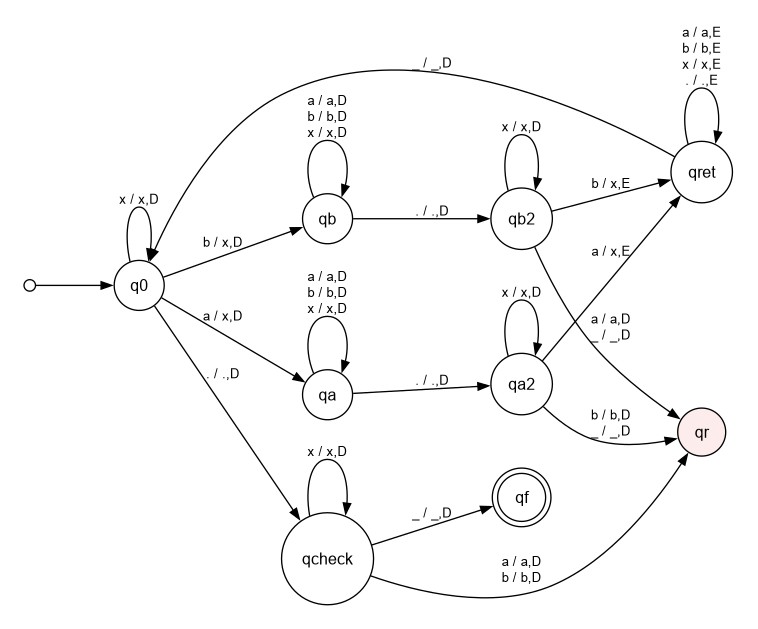
\includegraphics[width=0.8\linewidth,height=\textheight,keepaspectratio]{chapters/images/mt-w.w.png}

}

\caption{\label{fig-mt-wptow}Máquina de Turing para
L=\{w.w\mid w\in\{a,b\}\^{}*\}.}

\end{figure}%

Considere a entrada

\[
ab.ab
\]

A configuração inicial é

\[
C_0=\langle\_,q_0,ab.ab\rangle,
\]

em que \(\_\) representa o símbolo branco da fita. A máquina está no
estado inicial \(q_0\) e o cabeçote encontra-se sobre o primeiro símbolo
\(a\).

A máquina encontra um \(a\), marca esse símbolo com \(x\) e passa para
um estado que representa a busca pelo \(a\) correspondente na segunda
parte:

\[
C_0
=
\langle\_,q_0,ab.ab\rangle
\]

\[
\vdash
\langle \_x,q_a,b.ab\rangle
\]

A partir desse ponto, a máquina percorre a primeira parte da palavra até
encontrar o separador \texttt{.} e, em seguida, procura o primeiro
símbolo ainda não marcado na segunda parte. Ao encontrar o \(a\)
correspondente, marca-o com \(x\):

\[
\langle\_x,q_a,b.ab\rangle
\vdash^*
\langle \_xb.,q_{a2},ab\rangle
\]

\[
\vdash
\langle \_xb,q_{ret},.xb\rangle.
\]

O símbolo \(a\) da segunda parte foi, portanto, marcado. A máquina
retorna ao início da fita para procurar o próximo símbolo ainda não
processado na primeira parte:

\[
\langle\_xb,q_{ret},.xb\rangle
\vdash^*
\langle\_,q_0,xb.xb\rangle.
\]

Agora o primeiro símbolo ainda não marcado da primeira parte é \(b\). A
máquina o substitui por \(x\):

\[
\langle\_,q_0,xb.xb\rangle
\vdash^*
\langle\_xx,q_b,.xb\rangle
\]

Ela percorre novamente a fita até a segunda parte e procura o primeiro
símbolo ainda não marcado. Nesse caso, encontra \(b\), que corresponde
ao símbolo armazenado implicitamente no estado:

\[
\vdash^*
\langle\_xx,q_b,.xb\rangle
\vdash^*
\langle\_xx.x,q_{b2},b\rangle
\]

\[
\vdash
\langle\_xx.,q_{ret},xx\rangle
\]

A máquina retorna novamente ao início da fita. Nesse momento, todos os
símbolos da primeira parte e todos os símbolos correspondentes da
segunda parte estão marcados:

\[
\langle\_xx.,q_{ret},xx\rangle
\vdash^*
\langle\_,q_0,xx.xx\rangle
\]

Ao percorrer a primeira parte, a máquina não encontra mais símbolos
\(a\) ou \(b\) não marcados e encontra o separador \texttt{.}. \[
\langle\_,q_0,xx.xx\rangle
\vdash^*
\langle\_xx.,q_{check},xx\rangle
\]

Ela então verifica a segunda parte. Como também não existem símbolos não
marcados após o separador, a máquina entra no estado de aceitação: \[
\langle\_xx.,q_{check},xx\rangle
\vdash^*
\langle\_xx.xx\_,q_{f},\_\rangle
\]

Assim, a computação termina em um estado de aceitação e, portanto,

\[
ab.ab\in L.
\]

A sequência pode ser resumida por

\[
\begin{aligned}
\langle\_,q_0,ab.ab\rangle
&\vdash^*
\langle\_,q_0,xb.xb\rangle
&\vdash^*
\langle\_,q_0,xx.xx\rangle
&\vdash^*
\langle\_xx.xx\_,q_{f},\_\rangle
\end{aligned}
\]

O símbolo \(\vdash^*\) representa uma ou mais aplicações da relação de
sucessão entre configurações. Dessa forma, é possível omitir os passos
intermediários em que a máquina simplesmente percorre a fita,
concentrando a representação nos momentos relevantes da computação.

No simulador, esses passos podem ser acompanhados individualmente. A
cada execução de uma transição, a configuração instantânea é atualizada,
mostrando o estado corrente, o conteúdo da fita e a posição do cabeçote.
Simultaneamente, a transição correspondente pode ser destacada no
diagrama da máquina.

Esse exemplo evidencia uma característica fundamental da Máquina de
Turing: a fita funciona não apenas como meio de armazenamento da
entrada, mas também como \textbf{memória de trabalho}. O símbolo
auxiliar \(x\) permite registrar quais posições já foram processadas,
enquanto os estados da máquina permitem controlar qual símbolo deve ser
procurado na segunda parte da entrada.

A mesma estratégia permite identificar palavras que não pertencem à
linguagem. Por exemplo, para a entrada

\[
ab.ba,
\]

a máquina marca inicialmente o \(a\) da primeira parte e procura um
\(a\) na segunda parte. Como o primeiro símbolo não marcado encontrado
após o separador é \(b\), ocorre uma incompatibilidade e a máquina entra
no estado de rejeição.

\subsection{Reconhecimento e decisão}\label{reconhecimento-e-decisuxe3o}

A possibilidade de uma Máquina de Turing permanecer executando
indefinidamente leva a uma distinção importante. Uma linguagem é
denominada \textbf{Turing-reconhecível} quando existe uma Máquina de
Turing capaz de reconhecê-la. Isso significa que, para uma cadeia
pertencente à linguagem, a máquina eventualmente entra no estado de
aceitação. Para cadeias que não pertencem à linguagem, entretanto, a
máquina pode rejeitar ou pode continuar executando indefinidamente.

Uma linguagem é denominada \textbf{Turing-decidível} quando existe uma
Máquina de Turing que sempre termina sua computação, aceitando ou
rejeitando a entrada. Portanto, toda linguagem decidível é também
Turing-reconhecível, mas uma linguagem Turing-reconhecível não precisa
ser decidível.

Essa distinção será retomada na seção dedicada à
\textbf{decidibilidade}, na qual será estudado o problema de determinar
quais problemas podem ser resolvidos por um algoritmo que sempre
termina. O problema da parada, em particular, mostrará que existem
problemas para os quais não existe uma Máquina de Turing capaz de
produzir uma decisão correta para todas as entradas e sempre terminar
sua computação.

\subsection{Simulador de Máquina de
Turing}\label{simulador-de-muxe1quina-de-turing}

O simulador apresentado a seguir permite visualizar, de forma
interativa, o funcionamento de uma Máquina de Turing. Inicialmente, o
usuário pode definir os principais elementos da máquina: o conjunto de
estados, o alfabeto de entrada, o alfabeto da fita, o estado inicial, o
estado de aceitação e o estado de rejeição.

A partir dessas informações, o simulador permite construir a
\textbf{tabela de transição}, que representa a função de transição da
máquina. Para cada combinação de estado atual e símbolo lido na fita, a
tabela especifica o estado para o qual a máquina deve transitar, o
símbolo que deve ser escrito na posição corrente da fita e o movimento
realizado pelo cabeçote. O cabeçote pode se deslocar uma posição para a
\textbf{direita}, uma posição para a \textbf{esquerda} ou
\textbf{permanecer na mesma posição}.

Após o preenchimento da tabela de transição, o simulador gera
automaticamente o \textbf{diagrama da Máquina de Turing}, permitindo
visualizar graficamente seus estados e transições.

Por fim, o usuário pode fornecer uma palavra de entrada para realizar a
simulação da computação. A execução pode ser acompanhada passo a passo,
permitindo observar a transição realizada em cada etapa e a respectiva
\textbf{configuração instantânea} da máquina. Dessa forma, o simulador
relaciona a representação formal da máquina --- por meio da tabela de
transição --- com sua representação gráfica e com o processo efetivo de
computação sobre uma palavra de entrada.

\begin{figure}[H]
\centering
\fbox{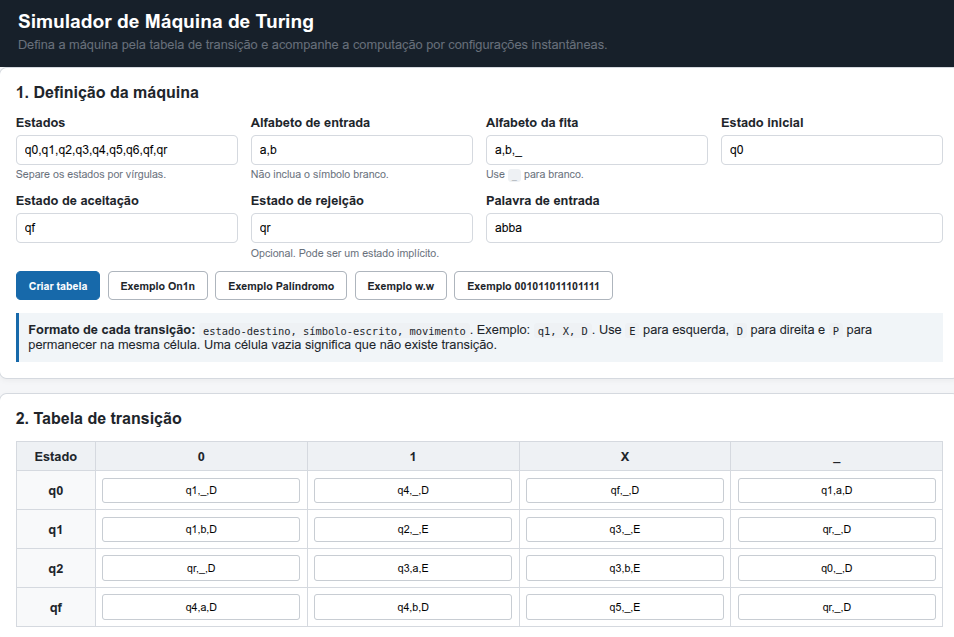
\includegraphics[width=0.6\textwidth]{chapters/images/printscreen/mt.png}}
\caption{Visualização da aplicação interativa}
\end{figure}
\begin{tcolorbox}[enhanced jigsaw, title=Acesso Interativo]
Acesse a simulação em:\par\smallskip
\small\url{https://luizedsilva.github.io/Livro-LTC/p5js/mt/}
\begin{center}
\includegraphics[width=3cm]{chapters/images/qrcode/mt.png}\end{center}
\end{tcolorbox}

\subsection{Decidibilidade}\label{decidibilidade}

A teoria da computação investiga os problemas que podem ser resolvidos
por algoritmos e os limites do processamento automático de informações.
Embora os computadores sejam capazes de executar uma enorme variedade de
tarefas, nem todo problema formulado de maneira precisa pode ser
resolvido por um algoritmo que produza uma resposta correta em tempo
finito para qualquer entrada.

O estudo da \textbf{decidibilidade} procura estabelecer quais problemas
admitem uma solução algorítmica completa. Para isso, utiliza-se um
modelo formal de computação, como a máquina de Turing, que permite
descrever algoritmos independentemente de uma linguagem de programação
ou de uma arquitetura específica. O aprofundamento sobre o tema da
decidibilidade e da computabilidade são apresentados em Sipser (2012),
Hopcroft; Motwani; Ullman (2007) e Kozen (1997).

A investigação da decidibilidade possui duas vertentes complementares. A
primeira consiste em demonstrar que determinado problema pode ser
resolvido, apresentando um algoritmo que sempre termina e fornece a
resposta correta. A segunda consiste em demonstrar que nenhum algoritmo
pode resolver o problema em todas as situações possíveis.

Conhecer os problemas indecidíveis é tão importante quanto conhecer
aqueles que podem ser resolvidos. Esse conhecimento permite reconhecer
os limites da automação, avaliar o que pode ser verificado por
ferramentas de análise de programas e compreender por que determinadas
tarefas não admitem uma solução geral. Além disso, a identificação
desses limites estimula a busca por soluções alternativas, como
algoritmos que funcionam apenas para classes restritas de entradas ou
procedimentos que fornecem respostas em determinadas situações, sem
garantir uma resposta para todas elas.

\subsubsection{Problemas de decisão e linguagens
decidíveis}\label{problemas-de-decisuxe3o-e-linguagens-deciduxedveis}

Um problema de decisão é um problema cuja resposta pode ser expressa por
uma das duas possibilidades: \textbf{sim} ou \textbf{não}. Por exemplo,
dado um número inteiro, verificar se ele é par constitui um problema de
decisão. Na teoria de linguagens, muitos problemas podem ser formulados
como perguntas sobre a pertinência de uma cadeia a uma linguagem.

Seja uma linguagem \(A\) sobre um alfabeto \(\Sigma\). O problema de
decisão associado a \(A\) consiste em determinar, para uma cadeia de
entrada \(w\in\Sigma^*\), se \(w\in A\).

Uma máquina de Turing pode ser utilizada para resolver esse problema.
Quando a máquina aceita \(w\), a resposta é positiva; quando rejeita
\(w\), a resposta é negativa. Entretanto, não basta que a máquina
forneça a resposta correta quando termina: é necessário garantir que ela
termine para toda entrada.

\begin{definition}[]\protect\hypertarget{def-decidivel}{}\label{def-decidivel}

Uma linguagem \(A\) é decidível se existe uma máquina de Turing que,
para toda entrada \(w\), termina sua execução e satisfaz as seguintes
condições:

\begin{itemize}
\tightlist
\item
  se \(w\in A\), a máquina aceita \(w\);
\item
  se \(w\notin A\), a máquina rejeita \(w\).
\end{itemize}

\end{definition}

Uma máquina de Turing que satisfaz essas condições é denominada
\emph{decisor} para \(A\).

A condição de término é essencial. Considere uma máquina que aceita
todas as cadeias pertencentes a \(A\), mas entra em um laço infinito
quando recebe uma cadeia que não pertence a \(A\). Essa máquina não
decide \(A\), pois não fornece uma resposta negativa em tempo finito.

A decidibilidade não exige que o algoritmo seja eficiente. Um decisor
pode realizar uma quantidade muito grande de operações e ainda assim
decidir a linguagem, desde que termine para toda entrada. A questão da
eficiência computacional é estudada principalmente pela teoria da
complexidade, enquanto a decidibilidade investiga inicialmente a
existência de um procedimento que sempre forneça uma resposta.

\paragraph{Linguagens reconhecíveis}\label{linguagens-reconhecuxedveis}

Uma linguagem \(A\) é \emph{Turing-reconhecível} se existe uma máquina
de Turing que aceita toda cadeia pertencente a \(A\). Para as cadeias
que não pertencem a \(A\), a máquina pode rejeitar ou executar
indefinidamente.

Portanto, toda linguagem decidível é Turing-reconhecível, mas a
recíproca não é verdadeira.

A diferença pode ser resumida da seguinte maneira:

\begin{longtable*}[]{|
  >{\raggedright\arraybackslash}p{(\linewidth - 6\tabcolsep - 4\arrayrulewidth) * \real{0.3333}}|
  >{\raggedright\arraybackslash}p{(\linewidth - 6\tabcolsep - 4\arrayrulewidth) * \real{0.3333}}|
  >{\raggedright\arraybackslash}p{(\linewidth - 6\tabcolsep - 4\arrayrulewidth) * \real{0.3333}}|}
\toprule\noalign{}
\begin{minipage}[b]{\linewidth}\smallskip
\raggedright
Tipo de máquina
\end{minipage} & \begin{minipage}[b]{\linewidth}\raggedright
Entrada pertencente à linguagem
\end{minipage} & \begin{minipage}[b]{\linewidth}\raggedright
Entrada não pertencente à linguagem
\end{minipage} \\
\midrule\noalign{}
\endhead
\bottomrule\noalign{}
\endlastfoot
Decisor & Aceita e termina & Rejeita e termina \\
\midrule
Reconhecedor & Aceita e termina & Rejeita ou não termina \\
\end{longtable*}

Essa distinção será fundamental para compreender o problema da parada,
que demonstra a existência de linguagens reconhecíveis que não são
decidíveis.

\subsubsection{Decidibilidade para linguagens
regulares}\label{decidibilidade-para-linguagens-regulares}

As linguagens regulares possuem propriedades que facilitam a construção
de algoritmos de decisão. Uma linguagem regular pode ser representada
por um autômato finito determinístico (AFD), um autômato finito não
determinístico (AFN) ou uma expressão regular. Como esses formalismos
possuem procedimentos efetivos de conversão e análise, vários problemas
envolvendo linguagens regulares são decidíveis.

\paragraph{Problema de aceitação para
AFDs}\label{problema-de-aceitauxe7uxe3o-para-afds}

Considere o problema de determinar se um autômato finito determinístico
aceita uma determinada cadeia. Seja

\[
A_{\mathrm{AFD}}=\{\langle B,w\rangle\mid B\text{ é um AFD que aceita }w\}.
\]

A notação \(\langle B,w\rangle\) representa uma codificação da descrição
do autômato \(B\) e da cadeia \(w\). Dessa forma, o problema pode ser
tratado como uma linguagem: uma codificação pertence a
\(A_{\mathrm{AFD}}\) se, e somente se, o autômato descrito aceita a
cadeia fornecida.

\begin{theorem}[]\protect\hypertarget{thm-afd}{}\label{thm-afd}

A linguagem \(A_{\mathrm{AFD}}\) é decidível.

\end{theorem}

\textbf{Demonstração.} Constrói-se uma máquina de Turing \(M_1\) que
recebe como entrada \(\langle B,w\rangle\) e executa as seguintes
etapas:

\begin{enumerate}
\def\labelenumi{\arabic{enumi}.}
\tightlist
\item
  Verifica se a entrada contém uma codificação válida de um AFD e de uma
  cadeia. Se não contiver, rejeita.
\item
  Simula a execução de \(B\) sobre \(w\), começando no estado inicial e
  consumindo os símbolos de \(w\), um a um.
\item
  Ao terminar a leitura da cadeia, verifica o estado alcançado.
\item
  Aceita se o estado for de aceitação; caso contrário, rejeita.
\end{enumerate}

A simulação termina porque um AFD realiza uma transição para cada
símbolo consumido e a cadeia de entrada possui comprimento finito.
Consequentemente, \(M_1\) sempre termina e fornece a resposta correta.
Logo, \(A_{\mathrm{AFD}}\) é decidível.

Esse resultado mostra que verificar a aceitação de uma cadeia por um AFD
é um problema decidível. Não é necessário examinar todas as cadeias
possíveis: basta simular o autômato sobre a cadeia específica fornecida.

\paragraph{Problema de aceitação para
AFNs}\label{problema-de-aceitauxe7uxe3o-para-afns}

Um autômato finito não determinístico pode possuir várias transições
possíveis para um mesmo símbolo e estado, além de transições vazias, que
não consomem símbolos da entrada. Assim, a aceitação ocorre quando
existe pelo menos um caminho de execução que termina em um estado de
aceitação após consumir toda a cadeia.

Considere a linguagem

\[
A_{\mathrm{AFN}}=\{\langle B,w\rangle\mid B\text{ é um AFN que aceita }w\}.
\]

\begin{theorem}[]\protect\hypertarget{thm-afn}{}\label{thm-afn}

A linguagem \(A_{\mathrm{AFN}}\) é decidível.

\end{theorem}

\textbf{Demonstração.} Seja \(M_2\) uma máquina de Turing que recebe
\(\langle B,w\rangle\), em que \(B\) é um AFN.

\begin{enumerate}
\def\labelenumi{\arabic{enumi}.}
\tightlist
\item
  Converte \(B\) em um AFD equivalente \(C\), utilizando a construção
  dos subconjuntos. Quando necessário, a construção considera os
  fechos-\(\varepsilon\) dos estados.
\item
  Executa \(M_1\) sobre a entrada \(\langle C,w\rangle\).
\item
  Produz a mesma resposta obtida por \(M_1\): aceita se \(C\) aceita
  \(w\) e rejeita caso contrário.
\end{enumerate}

A conversão de um AFN em um AFD é um procedimento efetivo que termina, e
os dois autômatos reconhecem a mesma linguagem. Como \(M_1\) é um
decisor, \(M_2\) também termina para toda entrada válida e responde
corretamente. Portanto, \(A_{\mathrm{AFN}}\) é decidível.

A demonstração utiliza uma estratégia recorrente na teoria da
computação: transformar um problema em outro problema já conhecido como
decidível. Como a conversão preserva a linguagem reconhecida, a resposta
obtida para o AFD resolve o problema original.

\paragraph{Problema de aceitação para expressões
regulares}\label{problema-de-aceitauxe7uxe3o-para-expressuxf5es-regulares}

Uma expressão regular representa uma linguagem regular por meio de
operações como união, concatenação e fecho de Kleene. Por isso, também é
possível decidir se uma cadeia pertence à linguagem representada por uma
expressão regular.

Definimos

\[
A_{\mathrm{ER}}=\{\langle R,w\rangle\mid R\text{ é uma expressão regular que aceita }w\}.
\]

\begin{theorem}[]\protect\hypertarget{thm-er}{}\label{thm-er}

A linguagem \(A_{\mathrm{ER}}\) é decidível.

\end{theorem}

\textbf{Demonstração.} Constrói-se uma máquina \(M_3\) que recebe
\(\langle R,w\rangle\) e executa os seguintes passos:

\begin{enumerate}
\def\labelenumi{\arabic{enumi}.}
\tightlist
\item
  Converte a expressão regular \(R\) em um AFN equivalente \(B\),
  utilizando construções para união, concatenação e fecho de Kleene.
\item
  Executa \(M_2\) sobre \(\langle B,w\rangle\).
\item
  Aceita se \(M_2\) aceitar e rejeita caso contrário.
\end{enumerate}

A conversão de uma expressão regular em um AFN termina e preserva a
linguagem representada. Como \(M_2\) decide o problema de aceitação para
AFNs, o procedimento também decide o problema para expressões regulares.

Assim, os três formalismos --- AFDs, AFNs e expressões regulares ---
permitem resolver o problema de pertinência de uma cadeia à linguagem
que representam.

\paragraph{Problema da vacuidade para
AFDs}\label{problema-da-vacuidade-para-afds}

Além de verificar se um autômato aceita uma cadeia específica, podemos
perguntar se ele aceita alguma cadeia. Esse é o problema da vacuidade,
também chamado de problema da linguagem vazia.

Seja

\[
V_{\mathrm{AFD}}=\{\langle A\rangle\mid A\text{ é um AFD e }L(A)=\varnothing\}.
\]

A linguagem \(L(A)\) é vazia quando não existe nenhuma cadeia aceita
pelo autômato.

\begin{theorem}[]\protect\hypertarget{thm-afd-vazio}{}\label{thm-afd-vazio}

A linguagem \(V_{\mathrm{AFD}}\) é decidível.

\end{theorem}

\textbf{Demonstração.} Constrói-se uma máquina de Turing \(M_4\) que
recebe a descrição de um AFD \(A\) e realiza uma busca nos estados
alcançáveis a partir do estado inicial:

\begin{enumerate}
\def\labelenumi{\arabic{enumi}.}
\tightlist
\item
  Marca o estado inicial de \(A\).
\item
  Repete o seguinte procedimento até que nenhum novo estado seja
  marcado: para cada estado já marcado, marca todos os estados
  alcançados por suas transições.
\item
  Verifica se algum estado de aceitação foi marcado.
\item
  Se nenhum estado de aceitação foi alcançado, aceita, indicando que
  \(L(A)=\varnothing\). Caso contrário, rejeita.
\end{enumerate}

A busca termina porque um AFD possui um número finito de estados. A cada
iteração, ou nenhum estado novo é marcado, ou pelo menos um estado
adicional passa a ser marcado. Como a quantidade de estados é finita, o
procedimento necessariamente termina.

Se nenhum estado de aceitação for alcançável a partir do estado inicial,
nenhuma cadeia poderá conduzir o autômato a um estado de aceitação.
Logo, sua linguagem é vazia. Se algum estado de aceitação for
alcançável, existe uma sequência de símbolos que conduz a esse estado, e
a linguagem não é vazia.

Portanto, \(M_4\) decide \(V_{\mathrm{AFD}}\).

O algoritmo não precisa enumerar todas as cadeias possíveis. Mesmo que
existam infinitas cadeias sobre o alfabeto do autômato, basta examinar a
estrutura finita de seus estados e transições.

\paragraph{Equivalência de AFDs}\label{equivaluxeancia-de-afds}

Dois autômatos são equivalentes quando reconhecem exatamente a mesma
linguagem. A equivalência pode ser expressa por

\[
L(A)=L(B).
\]

O problema consiste em determinar se dois AFDs reconhecem as mesmas
cadeias. Definimos

\[
EQ_{\mathrm{AFD}}=\{\langle A,B\rangle\mid A\text{ e }B\text{ são AFDs e }L(A)=L(B)\}.
\]

\begin{theorem}[]\protect\hypertarget{thm-eq-afd}{}\label{thm-eq-afd}

A linguagem \(EQ_{\mathrm{AFD}}\) é decidível.

\end{theorem}

\textbf{Demonstração.} A ideia consiste em verificar se existe alguma
cadeia aceita por apenas um dos dois autômatos. Para isso, constrói-se
um AFD \(C\) que reconhece a diferença simétrica das linguagens:

\[
\begin{aligned}
L(C)={}&(L(A)\cap\overline{L(B)})\\
&\cup(\overline{L(A)}\cap L(B)).
\end{aligned}
\]

A expressão \(\overline{L(A)}\) representa o complemento da linguagem de
\(A\), considerando o alfabeto de entrada adotado. A diferença simétrica
contém as cadeias que pertencem a uma das linguagens, mas não a ambas.

O procedimento de decisão é o seguinte:

\begin{enumerate}
\def\labelenumi{\arabic{enumi}.}
\tightlist
\item
  Constrói \(C\) utilizando as operações de complemento, interseção e
  união de linguagens regulares.
\item
  Executa \(M_4\) sobre \(\langle C\rangle\), verificando se
  \(L(C)=\varnothing\).
\item
  Se \(M_4\) aceitar, aceita a entrada original, pois não existe cadeia
  que diferencie os autômatos. Caso contrário, rejeita.
\end{enumerate}

Se \(L(C)=\varnothing\), não existe cadeia aceita por apenas um dos
autômatos, de modo que \(L(A)=L(B)\). Se \(L(C)\neq\varnothing\), existe
pelo menos uma cadeia que é aceita por um autômato e rejeitada pelo
outro.

Como as operações de construção de \(C\) são efetivas e \(M_4\) é um
decisor, o procedimento sempre termina. Portanto, \(EQ_{\mathrm{AFD}}\)
é decidível.

Esse exemplo ilustra outra técnica importante: um problema de
equivalência pode ser reduzido a um problema de vacuidade. Em vez de
comparar diretamente todos os elementos de duas linguagens, constrói-se
uma linguagem que representa suas diferenças e verifica-se se ela é
vazia.

\subsubsection{Decidibilidade para linguagens livres de
contexto}\label{decidibilidade-para-linguagens-livres-de-contexto}

As linguagens livres de contexto são reconhecidas por autômatos com
pilha e podem ser descritas por gramáticas livres de contexto (GLCs).
Embora algumas propriedades das linguagens regulares também sejam
decidíveis para linguagens livres de contexto, outras apresentam
dificuldades maiores.

Nesta seção, consideraremos três problemas: verificar se uma gramática
gera uma cadeia específica, verificar se a linguagem de uma gramática é
vazia e verificar se duas gramáticas geram a mesma linguagem.

\paragraph{Problema de pertinência para gramáticas livres de
contexto}\label{problema-de-pertinuxeancia-para-gramuxe1ticas-livres-de-contexto}

Seja \(G\) uma gramática livre de contexto e \(w\) uma cadeia. O
problema consiste em determinar se \(G\) gera \(w\), isto é, se existe
uma derivação

\[
S\Rightarrow^* w,
\]

em que \(S\) é o símbolo inicial da gramática e \(\Rightarrow^*\)
representa zero ou mais passos de derivação.

Definimos

\[
A_{\mathrm{GLC}}=\{\langle G,w\rangle\mid G\text{ é uma GLC que gera }w\}.
\]

\begin{theorem}[]\protect\hypertarget{thm-glc}{}\label{thm-glc}

A linguagem \(A_{\mathrm{GLC}}\) é decidível.

\end{theorem}

\textbf{Demonstração.} Constrói-se uma máquina de Turing \(M_6\) que
recebe \(\langle G,w\rangle\) e executa os seguintes passos:

\begin{enumerate}
\def\labelenumi{\arabic{enumi}.}
\tightlist
\item
  Converte \(G\) para a forma normal de Chomsky, preservando a linguagem
  gerada, com o tratamento apropriado para a cadeia vazia.
\item
  Se \(w\) possui comprimento \(n\geq 1\), enumera as derivações
  possíveis com \(2n-1\) passos de produção. Se \(w=\varepsilon\),
  verifica separadamente se a gramática gera a cadeia vazia.
\item
  Verifica se alguma das derivações enumeradas gera exatamente \(w\).
\item
  Aceita se encontrar uma derivação que gere \(w\); caso contrário,
  rejeita.
\end{enumerate}

Na forma normal de Chomsky, as produções são, em geral, da forma
\(A\rightarrow BC\) ou \(A\rightarrow a\), com uma produção especial
para a cadeia vazia quando ela pertence à linguagem. Para uma cadeia não
vazia de comprimento \(n\), uma derivação que a gera pode ser
representada por uma árvore de derivação com \(n\) folhas terminais e,
no caso binário, \(n-1\) nós internos. O número de produções utilizadas
é, portanto, \(2n-1\).

Como a gramática possui um número finito de produções, existe apenas um
número finito de derivações com esse limite de passos. Logo, a
enumeração termina. Se a cadeia pertence à linguagem, uma derivação
correspondente será encontrada; caso contrário, nenhuma derivação
enumerada produzirá a cadeia.

Assim, \(M_6\) termina para toda entrada e responde corretamente.
Portanto, \(A_{\mathrm{GLC}}\) é decidível.

A demonstração é baseada na existência de um limite finito para a busca.
A conversão para a forma normal de Chomsky restringe a estrutura das
derivações e torna possível examinar sistematicamente as alternativas em
um espaço finito.

\paragraph{Problema da vacuidade para gramáticas livres de
contexto}\label{problema-da-vacuidade-para-gramuxe1ticas-livres-de-contexto}

O problema da vacuidade para uma gramática livre de contexto consiste em
verificar se ela não gera nenhuma cadeia terminal. Definimos

\[
V_{\mathrm{GLC}}=\{\langle G\rangle\mid G\text{ é uma GLC e }L(G)=\varnothing\}.
\]

\begin{theorem}[]\protect\hypertarget{thm-glc-vazio}{}\label{thm-glc-vazio}

A linguagem \(V_{\mathrm{GLC}}\) é decidível.

\end{theorem}

\textbf{Demonstração.} A ideia é verificar se o símbolo inicial da
gramática pode gerar alguma cadeia composta exclusivamente por
terminais. Para isso, constrói-se uma máquina de Turing \(M_7\) que
realiza uma marcação progressiva dos símbolos da gramática:

\begin{enumerate}
\def\labelenumi{\arabic{enumi}.}
\tightlist
\item
  Marca todos os símbolos terminais.
\item
  Marca também qualquer variável \(A\) para a qual exista uma produção
  \(A\rightarrow U_1U_2\cdots U_k\) em que todos os símbolos do lado
  direito já estejam marcados. Uma produção \(A\rightarrow\varepsilon\)
  também permite marcar \(A\), pois seu lado direito não contém símbolos
  que precisem ser gerados.
\item
  Repete o procedimento até que nenhuma variável nova possa ser marcada.
\item
  Se a variável inicial não estiver marcada, aceita, indicando que a
  linguagem gerada é vazia. Caso contrário, rejeita.
\end{enumerate}

Uma variável marcada pode gerar uma cadeia formada somente por
terminais. Inicialmente, isso é verdadeiro para as produções cujos lados
direitos contêm apenas terminais ou são vazios. Em seguida, a
propriedade é propagada para as variáveis cujas produções dependem de
símbolos que já possuem essa capacidade.

Como a gramática possui um número finito de variáveis, o procedimento
não pode marcar novas variáveis indefinidamente. Portanto, termina.

Se o símbolo inicial for marcado, existe uma derivação que produz uma
cadeia terminal, e a linguagem não é vazia. Se não for marcado após o
encerramento do procedimento, nenhuma derivação a partir do símbolo
inicial poderá produzir uma cadeia terminal. Logo, a linguagem é vazia.

Portanto, \(M_7\) decide \(V_{\mathrm{GLC}}\).

\paragraph{Equivalência de gramáticas livres de
contexto}\label{equivaluxeancia-de-gramuxe1ticas-livres-de-contexto}

Duas gramáticas livres de contexto \(G\) e \(H\) são equivalentes quando
geram exatamente a mesma linguagem:

\[
L(G)=L(H).
\]

O problema de equivalência é definido por

\[
EQ_{\mathrm{GLC}}=\{\langle G,H\rangle\mid G\text{ e }H\text{ são GLCs e }L(G)=L(H)\}.
\]

\begin{theorem}[]\protect\hypertarget{thm-glc-eq}{}\label{thm-glc-eq}

A linguagem \(EQ_{\mathrm{GLC}}\) não é decidível.

\end{theorem}

Esse resultado estabelece um contraste importante entre linguagens
regulares e linguagens livres de contexto. Para AFDs, a equivalência
pode ser decidida por meio da construção da diferença simétrica e do
teste de vacuidade. Para gramáticas livres de contexto, não existe um
algoritmo geral que sempre termine e determine corretamente se duas
gramáticas arbitrárias geram a mesma linguagem.

A existência de algoritmos para decidir a pertinência de uma cadeia e a
vacuidade de uma gramática não implica que o problema de equivalência
também seja decidível. Cada problema precisa ser analisado
individualmente. Uma propriedade pode ser decidível enquanto outra,
aparentemente relacionada, é indecidível.

\paragraph{Toda linguagem livre de contexto é
decidível}\label{toda-linguagem-livre-de-contexto-uxe9-deciduxedvel}

Embora o problema de equivalência entre gramáticas livres de contexto
seja indecidível, toda linguagem livre de contexto é decidível.

\begin{theorem}[]\protect\hypertarget{thm-llc}{}\label{thm-llc}

Toda linguagem livre de contexto é uma linguagem decidível.

\end{theorem}

\textbf{Demonstração.} Seja \(A\) uma linguagem livre de contexto. Por
definição, existe uma gramática livre de contexto \(G\) tal que
\(L(G)=A\).

Construímos uma máquina de Turing \(M_8\) que recebe uma cadeia \(w\) e
executa o seguinte procedimento:

\begin{enumerate}
\def\labelenumi{\arabic{enumi}.}
\tightlist
\item
  Executa \(M_6\) sobre a entrada \(\langle G,w\rangle\).
\item
  Se \(M_6\) aceitar, aceita \(w\); caso contrário, rejeita \(w\).
\end{enumerate}

Como \(M_6\) decide se uma cadeia é gerada por uma gramática livre de
contexto, o procedimento sempre termina. Além disso, como \(L(G)=A\), a
cadeia \(w\) será aceita exatamente quando pertencer a \(A\).

Logo, \(M_8\) decide \(A\), e toda linguagem livre de contexto é
decidível.

Esse teorema mostra que o problema de pertinência para uma gramática
livre de contexto é decidível, mesmo que a equivalência entre duas
gramáticas livres de contexto não seja. É importante distinguir a
pergunta ``esta cadeia pertence à linguagem?'' da pergunta ``estas duas
gramáticas geram exatamente a mesma linguagem?''.

\subsection{O problema da parada}\label{o-problema-da-parada}

Até aqui, foram apresentados problemas para os quais é possível
construir máquinas de Turing que sempre terminam. Entretanto, nem todo
problema de decisão admite um decisor. A existência de problemas
indecidíveis estabelece um limite fundamental para o que pode ser
resolvido algoritmicamente.

Um dos resultados mais importantes da teoria da computação é a
indecidibilidade do problema da parada. Ele demonstra que não existe um
algoritmo geral capaz de determinar corretamente, para qualquer programa
ou máquina de Turing e qualquer entrada, se a execução terminará.

Esse resultado tem consequências relevantes para a análise automática de
programas. Por exemplo, não existe um procedimento geral que, para
qualquer programa arbitrário e qualquer entrada, determine sempre se sua
execução terminará. Isso não significa que seja impossível analisar
programas específicos: muitos programas podem ser verificados por
métodos estáticos, testes ou análises especializadas. O limite está na
existência de uma solução geral que funcione corretamente para todos os
casos.

\subsubsection{O problema de aceitação para máquinas de
Turing}\label{o-problema-de-aceitauxe7uxe3o-para-muxe1quinas-de-turing}

Considere a linguagem

\[
A_{\mathrm{MT}}=\{\langle M,w\rangle\mid M\text{ é uma MT que aceita }w\}.
\]

A entrada contém a descrição de uma máquina de Turing \(M\) e uma cadeia
\(w\). A pergunta é se \(M\), quando executada sobre \(w\), alcançará um
estado de aceitação.

\begin{theorem}[]\protect\hypertarget{thm-mt}{}\label{thm-mt}

A linguagem \(A_{\mathrm{MT}}\) é Turing-reconhecível, mas não é
decidível.

\end{theorem}

Para compreender a primeira parte do teorema, construímos uma máquina de
Turing universal \(U\), capaz de simular a execução de outra máquina
descrita na entrada.

A máquina \(U\) recebe \(\langle M,w\rangle\) e executa os seguintes
passos:

\begin{enumerate}
\def\labelenumi{\arabic{enumi}.}
\tightlist
\item
  Simula \(M\) sobre a entrada \(w\).
\item
  Se \(M\) entrar em um estado de aceitação, aceita.
\item
  Se \(M\) entrar em um estado de rejeição, rejeita.
\item
  Se \(M\) continuar executando indefinidamente, a simulação também
  continuará indefinidamente.
\end{enumerate}

Esse procedimento reconhece \(A_{\mathrm{MT}}\), pois aceita todas as
entradas em que a máquina simulada aceita a cadeia. Contudo, ele não é
um decisor: quando \(M\) entra em um laço infinito, \(U\) também não
termina.

A existência desse reconhecedor demonstra que \(A_{\mathrm{MT}}\) é
Turing-reconhecível. Para concluir que a linguagem não é decidível, é
necessário demonstrar que nenhum outro algoritmo poderia resolver o
problema em todos os casos.

\subsubsection{O problema da parada e sua relação com a
aceitação}\label{o-problema-da-parada-e-sua-relauxe7uxe3o-com-a-aceitauxe7uxe3o}

O problema da parada pergunta se uma máquina de Turing termina sua
execução sobre determinada entrada, independentemente de aceitar ou
rejeitar. Sua linguagem pode ser definida por

\[
HALT_{\mathrm{MT}}=\{\langle M,w\rangle\mid M\text{ termina sua execução sobre }w\}.
\]

O problema de aceitação \(A_{\mathrm{MT}}\) e o problema da parada
\(HALT_{\mathrm{MT}}\) são relacionados, mas não são idênticos.

Se \(M\) aceita \(w\), então \(M\) necessariamente termina sua execução.
Entretanto, se \(M\) não aceita \(w\), existem duas possibilidades: ela
pode rejeitar a entrada e terminar, ou pode executar indefinidamente.

Assim, a simulação direta permite reconhecer a aceitação, mas não
permite decidir em todos os casos se a máquina terminará. Nos dois
problemas, a dificuldade está em lidar com execuções que podem continuar
para sempre.

Os dois problemas são indecidíveis. A seguir, será demonstrada a
indecidibilidade de \(A_{\mathrm{MT}}\), utilizando um argumento por
contradição e autorreferência.

\subsubsection{Demonstração da indecidibilidade do problema de
aceitação}\label{demonstrauxe7uxe3o-da-indecidibilidade-do-problema-de-aceitauxe7uxe3o}

Suponha, por contradição, que exista uma máquina de Turing \(H\) capaz
de decidir \(A_{\mathrm{MT}}\). Isso significa que \(H\) recebe uma
codificação \(\langle M,w\rangle\) e sempre termina, respondendo
corretamente:

\begin{itemize}
\tightlist
\item
  aceita se \(M\) aceita \(w\);
\item
  rejeita se \(M\) não aceita \(w\), seja porque rejeita ou porque sua
  execução não termina.
\end{itemize}

A segunda condição é mais forte do que simplesmente simular \(M\). A
máquina \(H\) teria que fornecer uma resposta negativa mesmo nos casos
em que \(M\) entra em um laço infinito.

Com base nessa hipótese, construiremos uma nova máquina de Turing \(D\),
que utiliza \(H\) como subrotina. A máquina \(D\) recebe a descrição de
uma máquina \(M\) e executa o seguinte procedimento:

\begin{enumerate}
\def\labelenumi{\arabic{enumi}.}
\tightlist
\item
  Executa \(H\) sobre a entrada \(\langle M,\langle M\rangle\rangle\),
  isto é, pergunta se \(M\) aceita sua própria descrição.
\item
  Se \(H\) responder que \(M\) aceita \(\langle M\rangle\), então \(D\)
  rejeita.
\item
  Se \(H\) responder que \(M\) não aceita \(\langle M\rangle\), então
  \(D\) aceita.
\end{enumerate}

Em outras palavras, \(D\) produz exatamente o contrário da resposta dada
por \(H\) quando a máquina analisada recebe sua própria descrição como
entrada.

A construção é válida porque a descrição de uma máquina de Turing pode
ser codificada como uma cadeia. Portanto, uma máquina pode receber e
processar a codificação de outra máquina, inclusive sua própria
codificação.

Como \(H\) foi suposto um decisor, ele sempre termina. Consequentemente,
\(D\) também termina para toda entrada válida: após executar \(H\),
basta inverter sua resposta.

Agora, consideremos o que acontece quando \(D\) recebe sua própria
descrição \(\langle D\rangle\).

Existem apenas duas possibilidades.

\textbf{Caso 1: \(D\) aceita \(\langle D\rangle\).}

Como \(H\) deveria decidir corretamente o problema de aceitação, ele
responderia que \(D\) aceita sua própria descrição. Entretanto, pela
definição de \(D\), quando \(H\) responde que a máquina aceita, \(D\)
deve rejeitar. Portanto, \(D\) rejeita \(\langle D\rangle\),
contradizendo a hipótese inicial deste caso.

\textbf{Caso 2: \(D\) rejeita \(\langle D\rangle\).}

Nesse caso, \(H\) responderia que \(D\) não aceita sua própria
descrição. Pela definição de \(D\), quando \(H\) responde que a máquina
não aceita, \(D\) deve aceitar. Portanto, \(D\) aceita
\(\langle D\rangle\), contradizendo novamente a hipótese inicial.

Nos dois casos, obtemos uma contradição. Logo, a hipótese de que \(H\)
existe é falsa.

Concluímos que não existe uma máquina de Turing que decida
\(A_{\mathrm{MT}}\). Portanto, o problema de aceitação para máquinas de
Turing é indecidível.

\subsubsection{Por que o argumento
funciona?}\label{por-que-o-argumento-funciona}

A demonstração utiliza três ideias fundamentais.

A primeira é a hipótese de que existe um decisor universal para o
problema de aceitação. Esse decisor deveria analisar qualquer máquina e
qualquer entrada, sempre terminando com uma resposta correta.

A segunda é a construção de uma máquina que consulta o decisor e inverte
sua resposta. A máquina \(D\) não tenta prever diretamente o
comportamento de todas as máquinas: ela utiliza a suposta solução geral
e age deliberadamente de maneira contrária ao resultado informado.

A terceira é a autorreferência. Ao executar \(D\) sobre sua própria
descrição, fazemos com que a máquina seja analisada exatamente no caso
para o qual foi construída para contrariar a resposta do decisor.

A contradição não decorre de uma falha na execução de \(D\). Pelo
contrário, se \(H\) existisse, \(D\) seria um procedimento bem definido
e terminaria para toda entrada. O problema está na impossibilidade de
existir um decisor \(H\) com as propriedades supostas.

É importante observar que o argumento não demonstra que nenhuma máquina
pode analisar qualquer outra máquina. Máquinas podem simular outras
máquinas, verificar comportamentos particulares e decidir várias
propriedades de programas. O que a demonstração exclui é a existência de
um decisor geral para o problema de aceitação.

\subsubsection{Indecidibilidade do problema da
parada}\label{indecidibilidade-do-problema-da-parada}

O problema da parada também é indecidível. Esse resultado pode ser
obtido a partir da indecidibilidade do problema de aceitação.

Suponha que existisse um decisor \(K\) para \(HALT_{\mathrm{MT}}\),
capaz de determinar se uma máquina \(M\) termina sua execução sobre uma
entrada \(w\).

Poderíamos utilizar \(K\) para construir um decisor para
\(A_{\mathrm{MT}}\):

\begin{enumerate}
\def\labelenumi{\arabic{enumi}.}
\tightlist
\item
  Recebe \(\langle M,w\rangle\) e executa \(K\) para determinar se \(M\)
  termina sobre \(w\).
\item
  Se \(K\) responder que \(M\) não termina, rejeita, pois uma execução
  infinita não pode aceitar.
\item
  Se \(K\) responder que \(M\) termina, simula \(M\) sobre \(w\) até que
  a execução termine.
\item
  Aceita se \(M\) aceitar e rejeita se \(M\) rejeitar.
\end{enumerate}

Esse procedimento sempre terminaria. No primeiro caso, \(K\) já
forneceria a resposta negativa. No segundo, a resposta de \(K\)
garantiria que a simulação terminaria. Assim, obteríamos um decisor para
\(A_{\mathrm{MT}}\).

Entretanto, já demonstramos que \(A_{\mathrm{MT}}\) é indecidível.
Portanto, a suposição de que \(K\) existe leva a uma contradição.

Concluímos que o problema da parada é indecidível.

Esse argumento é um exemplo de redução entre problemas: se um problema
indecidível pudesse ser resolvido por meio de um decisor para outro
problema, então a existência desse decisor também resolveria o problema
indecidível. Como isso é impossível, o decisor suposto não pode existir.

\subsection{Síntese dos resultados}\label{suxedntese-dos-resultados}

Os resultados apresentados mostram que a decidibilidade depende da
natureza do problema analisado. Não basta identificar o formalismo
utilizado; é necessário especificar a propriedade que se deseja
verificar.

\begin{longtable*}[]{|l|l|}
\toprule\noalign{}
Problema & Resultado \\
\midrule\noalign{}
\endhead
\bottomrule\noalign{}
\endlastfoot
Aceitação de uma cadeia por um AFD & Decidível \\
\midrule
Aceitação de uma cadeia por um AFN & Decidível \\
\midrule
Aceitação de uma cadeia por uma expressão regular & Decidível \\
\midrule
Vacuidade da linguagem de um AFD & Decidível \\
\midrule
Equivalência entre dois AFDs & Decidível \\
\midrule
Pertinência de uma cadeia a uma GLC & Decidível \\
\midrule
Vacuidade da linguagem de uma GLC & Decidível \\
\midrule
Equivalência entre duas GLCs & Indecidível \\
\midrule
Aceitação para máquinas de Turing & Indecidível \\
\midrule
Problema da parada para máquinas de Turing & Indecidível \\
\end{longtable*}

A comparação entre esses resultados evidencia duas conclusões. Primeiro,
a existência de uma representação finita de uma linguagem não garante,
por si só, que toda propriedade de interesse seja decidível. Segundo, a
decidibilidade de um problema não implica a decidibilidade de todos os
problemas relacionados.

Para linguagens regulares, os procedimentos de conversão entre
formalismos, as operações de fechamento e a análise de grafos finitos
permitem resolver diversos problemas. Para linguagens livres de
contexto, o problema de pertinência e o problema da vacuidade são
decidíveis, mas a equivalência entre gramáticas livres de contexto é
indecidível. Para máquinas de Turing, a indecidibilidade do problema de
aceitação e do problema da parada demonstra limites fundamentais da
computação.

\subsection{Considerações finais}\label{considerauxe7uxf5es-finais}

A decidibilidade constitui um dos conceitos centrais da teoria da
computação, pois permite distinguir os problemas para os quais existe um
algoritmo geral que sempre termina daqueles para os quais tal algoritmo
não pode existir.

A construção de decisores, como os apresentados para linguagens
regulares e livres de contexto, demonstra como procedimentos finitos
podem resolver problemas de pertinência, vacuidade e equivalência em
determinadas classes de linguagens. Em contrapartida, o argumento
diagonal utilizado no problema de aceitação mostra que nem toda questão
sobre o comportamento de uma máquina de Turing pode ser resolvida
algoritmicamente.

O problema da parada possui uma consequência especialmente relevante:
não existe um método geral que determine corretamente, para qualquer
programa e qualquer entrada, se sua execução terminará. Esse limite não
impede a análise de programas específicos, mas estabelece que nenhuma
solução geral pode cobrir todos os casos possíveis.

Portanto, compreender a decidibilidade é essencial tanto para o
desenvolvimento de algoritmos quanto para o estudo de linguagens
formais, compiladores e ferramentas de análise de programas. Antes de
procurar um algoritmo para um problema, é importante investigar se esse
algoritmo pode existir. Essa investigação permite reconhecer os limites
teóricos da computação e direcionar os esforços para métodos que sejam
efetivamente possíveis.

\section{Da Máquina de Turing à máquina
virtual}\label{da-muxe1quina-de-turing-uxe0-muxe1quina-virtual}

A máquina de Turing é um modelo formal utilizado para estudar o que pode
ser computado por meio de um procedimento algorítmico. Sua importância
está na possibilidade de descrever, de maneira abstrata, os passos de
uma computação, sem depender de uma arquitetura específica de computador
ou de uma linguagem de programação.

Na prática, entretanto, os programas escritos em linguagens de alto
nível não são executados diretamente por uma máquina de Turing. Para que
sejam executados em um computador real, é necessário traduzir suas
construções para instruções que possam ser interpretadas pelo
processador ou por outro ambiente de execução. Essa tradução é uma das
tarefas centrais de um compilador.

O objetivo principal de um compilador é transformar um programa escrito
em uma linguagem-fonte em uma representação equivalente que possa ser
executada por uma máquina-alvo. Em um compilador tradicional, essa
representação pode ser o código de máquina de uma arquitetura real. Como
as arquiteturas reais apresentam muitos detalhes, trabalhar diretamente
com suas instruções pode tornar o estudo da compilação excessivamente
complexo.

Uma alternativa didática consiste em definir uma máquina abstrata mais
simples, com memória, registradores e um conjunto reduzido de
instruções. Essa máquina serve como alvo para o compilador e permite
estudar a tradução de expressões, atribuições, comandos de seleção,
repetição e entrada e saída. Neste capítulo, será utilizada a
\textbf{Máquina Virtual Simples (MVS)}, baseada na Máquina de Execução
Pascal (MEPA), proposta por Tomás Kowaltowski.

A MVS não substitui a máquina de Turing como modelo teórico de
computação. Seu propósito é diferente: oferecer uma arquitetura
simplificada na qual se possa representar e executar o código produzido
por um compilador didático. A máquina de Turing permite raciocinar sobre
a computabilidade; a máquina virtual permite explorar, de forma
concreta, como as construções de uma linguagem de programação são
traduzidas em instruções executáveis.

\subsection{Da linguagem de alto nível à máquina
virtual}\label{da-linguagem-de-alto-nuxedvel-uxe0-muxe1quina-virtual}

Considere um programa escrito em uma linguagem de alto nível. Essa
linguagem permite expressar operações por meio de construções próximas
da maneira como os seres humanos descrevem algoritmos, como expressões
aritméticas, atribuições, comandos condicionais e laços de repetição.

O processador, por sua vez, executa instruções de baixo nível definidas
por sua arquitetura. A função do compilador é estabelecer uma tradução
entre essas duas representações, preservando o comportamento do
programa.

Em termos gerais, o processo pode ser representado por:

\[
\text{Programa-fonte}
\longrightarrow
\text{Compilador}
\longrightarrow
\text{Código-alvo}
\]

Quando o código-alvo é definido para uma arquitetura real, o compilador
precisa considerar detalhes como registradores físicos, modos de
endereçamento e conjunto de instruções. Para fins didáticos, podemos
substituir essa arquitetura por uma máquina virtual com um conjunto
pequeno e bem definido de operações.

Nesse cenário, o compilador traduz o programa-fonte para uma sequência
de instruções da MVS. Um interpretador ou simulador da máquina virtual
executa essas instruções, atualizando a memória e os registradores de
acordo com a semântica de cada operação.

A utilização de uma máquina virtual separa duas preocupações: a tradução
da linguagem de programação e a execução do código gerado. Essa
separação facilita o desenvolvimento e a compreensão de um compilador,
pois não exige a implementação imediata de código de máquina para um
processador específico.

\subsection{Organização da Máquina Virtual
Simples}\label{organizauxe7uxe3o-da-muxe1quina-virtual-simples}

A memória da MVS é dividida em duas regiões principais:

\begin{itemize}
\tightlist
\item
  \textbf{Memória de programa (\(P\)):} armazena a sequência de
  instruções do programa que está sendo executado.
\item
  \textbf{Memória de dados (\(M\)):} funciona como uma pilha na qual são
  armazenados os valores manipulados pelas instruções.
\end{itemize}

As duas regiões podem ser entendidas como vetores cujas posições são
identificadas por índices inteiros, a partir de zero, até um limite
definido pela implementação.

Além dessas regiões de memória, a MVS possui três registradores de
controle: \(i\), \(s\) e \(d\).

\begin{figure}

\centering{

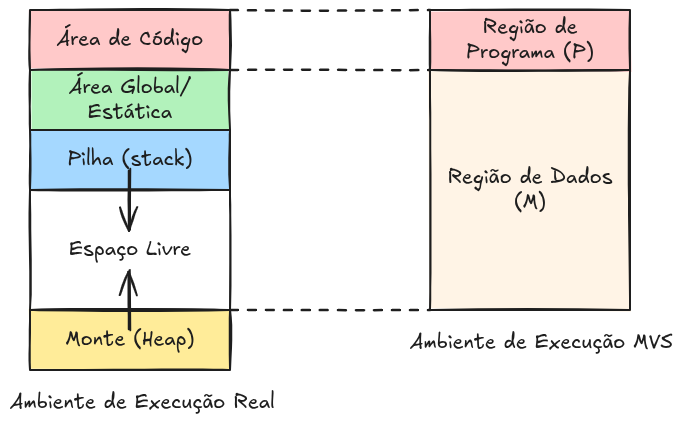
\includegraphics[width=0.6\linewidth,height=\textheight,keepaspectratio]{chapters/images/ambiente-mvs.png}

}

\caption{\label{fig-ambiente-mvs}Ambiente de execução da máquina virtual
simples (MVS)}

\end{figure}%

A Figura~\ref{fig-ambiente-mvs} compara a organização da memória em um
ambiente de execução de uma arquitetura real com a organização adotada
pela máquina virtual MVS.

No ambiente de execução real, a memória é organizada em diferentes
regiões: a área de código, a área global/estática, a pilha de execução
(stack) e a área de alocação dinâmica (heap). Entre a pilha e a área de
heap, pode existir um espaço livre compartilhado, permitindo que ambas
cresçam em direções opostas, conforme as necessidades da execução.

No ambiente de execução da MVS, essa organização é simplificada. A
região de programa \(P\) armazena as instruções do programa a ser
executado, enquanto a região de dados \(M\) reúne as informações
necessárias à execução. Essa região corresponde, conceitualmente, à
memória utilizada pela máquina virtual para representar os dados e
manter o estado de execução do programa.

Diferentemente do ambiente real ilustrado, a MVS não apresenta regiões
separadas para variáveis globais, pilha e heap. Sua estrutura
simplificada também não prevê um mecanismo específico de alocação
dinâmica de memória equivalente ao heap das arquiteturas reais.

\subsubsection{Registrador de
instrução}\label{registrador-de-instruuxe7uxe3o}

O registrador \(i\) contém o endereço da próxima instrução a ser
executada. Assim, a instrução corrente é obtida por meio de \(P[i]\).

Na execução normal, após uma instrução ser executada, o registrador
\(i\) é incrementado para apontar para a próxima posição do programa. As
instruções de desvio constituem uma exceção: elas alteram explicitamente
o valor de \(i\), transferindo o controle para outro endereço.

Essa organização permite representar a sequência de execução de um
programa como uma sucessão de posições da memória de programa. Em vez de
executar necessariamente as instruções na ordem em que aparecem, a
máquina pode saltar para outros trechos do código.

\subsubsection{Registrador de topo da
pilha}\label{registrador-de-topo-da-pilha}

O registrador \(s\) indica a posição ocupada pelo elemento que está no
topo da pilha de dados, isto é, \(M[s]\).

A pilha é utilizada para armazenar constantes, valores de variáveis e
resultados intermediários de expressões. As instruções que inserem um
valor na pilha incrementam \(s\); as que consomem operandos normalmente
diminuem esse registrador.

Na configuração inicial, a pilha está vazia e \(s=-1\). Dessa forma, a
primeira inserção incrementa \(s\) para zero e armazena o valor em
\(M[0]\).

A pilha simplifica a geração de código. Para calcular uma expressão, o
compilador pode produzir instruções que colocam os operandos na pilha e,
em seguida, executam uma operação que retira esses operandos e coloca o
resultado no lugar apropriado.

\subsubsection{Registrador de base}\label{registrador-de-base}

O registrador \(d\) contém um endereço de base utilizado no
endereçamento de variáveis. Nos exemplos apresentados, os endereços das
variáveis são fornecidos como operandos das instruções, e o registrador
de base permite generalizar o endereçamento de variáveis globais e
locais.

Essa organização está relacionada à necessidade de distinguir as
posições de memória associadas às variáveis. Durante a tradução, o
compilador atribui endereços às variáveis e utiliza esses endereços nas
instruções que leem ou armazenam seus valores.

\subsubsection{Estado da máquina}\label{estado-da-muxe1quina}

Em uma visão simplificada, a configuração da MVS é determinada pelo
conteúdo da memória de programa, pelo conteúdo da memória de dados e
pelos valores dos registradores. A execução de uma instrução transforma
essa configuração em outra.

Podemos representar essa ideia de forma abstrata por:

\[
C = (P,M,i,s,d)
\]

A execução de uma instrução modifica um ou mais componentes de \(C\).
Por exemplo, uma operação aritmética altera a pilha; uma instrução de
desvio modifica o registrador \(i\); e uma instrução de armazenamento
modifica uma posição da memória de dados.

Essa visão é semelhante à utilizada para descrever configurações
instantâneas em outros modelos de computação: o comportamento da máquina
pode ser compreendido como uma sequência de configurações produzidas
pela aplicação das regras de execução.

\subsection{Conjunto de instruções da
MVS}\label{conjunto-de-instruuxe7uxf5es-da-mvs}

As instruções da MVS são operações elementares que o compilador combina
para representar construções da linguagem-fonte. A seguir, elas são
organizadas por finalidade.

\subsubsection{Instruções de manipulação da pilha e da
memória}\label{instruuxe7uxf5es-de-manipulauxe7uxe3o-da-pilha-e-da-memuxf3ria}

\begin{longtable*}[]{|
  >{\raggedright\arraybackslash}p{(\linewidth - 4\tabcolsep - 3\arrayrulewidth) * \real{0.5000}}|
  >{\raggedright\arraybackslash}p{(\linewidth - 4\tabcolsep - 3\arrayrulewidth) * \real{0.5000}}|}
\toprule\noalign{}
\begin{minipage}[b]{\linewidth}\smallskip
\raggedright
Instrução
\end{minipage} & \begin{minipage}[b]{\linewidth}\raggedright
Significado
\end{minipage} \\
\midrule\noalign{}
\endhead
\bottomrule\noalign{}
\endlastfoot
\texttt{CRCT\ k} & Insere a constante \texttt{k} no topo da pilha. \\
\midrule
\texttt{CRVG\ n} & Lê o valor armazenado em \texttt{M{[}n{]}} e o insere
na pilha. \\
\midrule
\texttt{ARZG\ n} & Armazena em \texttt{M{[}n{]}} o valor do topo da
pilha e remove esse valor da pilha. \\
\midrule
\texttt{AMEM\ n} & Reserva espaço para \texttt{n} posições de dados,
avançando o topo da pilha. \\
\midrule
\texttt{DMEM\ n} & Desaloca \texttt{n} posições de dados na memória \\
\end{longtable*}

A instrução \texttt{CRCT\ k} executa as operações:

\[
s \leftarrow s+1
\]

\[
M[s] \leftarrow k
\]

Já a instrução \texttt{CRVG\ n} consulta a posição indicada pelo
operando e coloca uma cópia de seu conteúdo no topo da pilha:

\[
s \leftarrow s+1
\]

\[
M[s] \leftarrow M[n]
\]

A instrução \texttt{ARZG\ n} realiza o movimento inverso: utiliza o
valor que está no topo da pilha para atualizar uma posição de memória e,
depois, remove o valor consumido:

\[
M[n] \leftarrow M[s]
\]

\[
s \leftarrow s-1
\]

Essas três instruções são suficientes para carregar constantes,
consultar variáveis e armazenar resultados em variáveis. A instrução
\texttt{AMEM\ n} é usada na preparação do espaço de dados necessário
para as variáveis do programa. E por fim, a instrução \texttt{DMEM\ n}
decrementa o ponteiro da pilha em n posições, liberando o espaço
anteriormente utilizado por variáveis locais ou globais associados à
execução de um bloco (corpo principal do programa ou contexto local de
uma rotina).

Essa instrução permite controlar explicitamente o espaço ocupado pelos
dados durante a execução do programa.

\subsubsection{Instruções
aritméticas}\label{instruuxe7uxf5es-aritmuxe9ticas}

As operações aritméticas trabalham com os dois elementos que estão no
topo da pilha. O segundo elemento a partir do topo é combinado com o
elemento do topo, e o resultado ocupa a posição do primeiro operando. Em
seguida, o topo da pilha é reduzido em uma unidade.

\begin{longtable*}[]{|
  >{\raggedright\arraybackslash}p{(\linewidth - 4\tabcolsep - 3\arrayrulewidth) * \real{0.5000}}|
  >{\raggedright\arraybackslash}p{(\linewidth - 4\tabcolsep - 3\arrayrulewidth) * \real{0.5000}}|}
\toprule\noalign{}
\begin{minipage}[b]{\linewidth}\smallskip
\raggedright
Instrução
\end{minipage} & \begin{minipage}[b]{\linewidth}\raggedright
Operação
\end{minipage} \\
\midrule\noalign{}
\endhead
\bottomrule\noalign{}
\endlastfoot
\texttt{SOMA} & Soma os dois valores do topo da pilha. \\
\midrule
\texttt{SUBT} & Subtrai o valor do topo do valor imediatamente abaixo
dele. \\
\midrule
\texttt{MULT} & Multiplica os dois valores do topo da pilha. \\
\midrule
\texttt{DIVI} & Divide o valor imediatamente abaixo do topo pelo valor
do topo. \\
\end{longtable*}

Por exemplo, para \texttt{SOMA}, a atualização é:

\[
M[s-1] \leftarrow M[s-1] + M[s]
\]

\[
s \leftarrow s-1
\]

Para \texttt{SUBT}, a ordem dos operandos é importante:

\[
M[s-1] \leftarrow M[s-1] - M[s]
\]

\[
s \leftarrow s-1
\]

As operações de subtração e divisão não são comutativas. Por isso, a
ordem em que os operandos são colocados na pilha precisa corresponder à
estrutura da expressão original.

\subsubsection{Instruções relacionais e
lógicas}\label{instruuxe7uxf5es-relacionais-e-luxf3gicas}

As instruções relacionais comparam os dois valores do topo da pilha e
substituem os operandos por um resultado lógico. Nos exemplos da MVS, o
valor \texttt{1} representa verdadeiro e o valor \texttt{0} representa
falso.

\begin{longtable*}[]{|
  >{\raggedright\arraybackslash}p{(\linewidth - 4\tabcolsep - 3\arrayrulewidth) * \real{0.5000}}|
  >{\raggedright\arraybackslash}p{(\linewidth - 4\tabcolsep - 3\arrayrulewidth) * \real{0.5000}}|}
\toprule\noalign{}
\begin{minipage}[b]{\linewidth}\smallskip
\raggedright
Instrução
\end{minipage} & \begin{minipage}[b]{\linewidth}\raggedright
Significado
\end{minipage} \\
\midrule\noalign{}
\endhead
\bottomrule\noalign{}
\endlastfoot
\texttt{CMMA} & Compara se o valor abaixo do topo é maior que o valor do
topo. \\
\midrule
\texttt{CMME} & Compara se o valor abaixo do topo é menor que o valor do
topo. \\
\midrule
\texttt{CMIG} & Compara se os dois valores são iguais. \\
\midrule
\texttt{DISJ} & Calcula a disjunção lógica dos dois valores do topo. \\
\midrule
\texttt{CONJ} & Calcula a conjunção lógica dos dois valores do topo. \\
\midrule
\texttt{NEGA} & Inverte o valor lógico do topo da pilha. \\
\end{longtable*}

Para \texttt{CMMA}, por exemplo, a máquina compara \(M[s-1]\) e
\(M[s]\). Se \(M[s-1] > M[s]\), o resultado é \texttt{1}; caso
contrário, é \texttt{0}. O resultado ocupa a posição \(M[s-1]\), e o
topo da pilha diminui em uma unidade.

A instrução \texttt{NEGA} opera sobre um único valor lógico e pode ser
descrita por:

\[
M[s] \leftarrow 1-M[s]
\]

Considerando a representação de verdadeiro por \texttt{1} e falso por
\texttt{0}, essa operação transforma \texttt{1} em \texttt{0} e
\texttt{0} em \texttt{1}.

Essas instruções permitem traduzir as condições utilizadas em comandos
de seleção e repetição. A expressão lógica é avaliada primeiro; seu
resultado determina o caminho que será executado em seguida.

\subsubsection{Instruções de desvio}\label{instruuxe7uxf5es-de-desvio}

As instruções de desvio alteram o fluxo de execução do programa.

\begin{longtable*}[]{|
  >{\raggedright\arraybackslash}p{(\linewidth - 4\tabcolsep - 3\arrayrulewidth) * \real{0.5000}}|
  >{\raggedright\arraybackslash}p{(\linewidth - 4\tabcolsep - 3\arrayrulewidth) * \real{0.5000}}|}
\toprule\noalign{}
\begin{minipage}[b]{\linewidth}\smallskip
\raggedright
Instrução
\end{minipage} & \begin{minipage}[b]{\linewidth}\raggedright
Significado
\end{minipage} \\
\midrule\noalign{}
\endhead
\bottomrule\noalign{}
\endlastfoot
\texttt{DSVS\ p} & Desvia incondicionalmente para o endereço
\texttt{p}. \\
\midrule
\texttt{DSVF\ p} & Desvia para \texttt{p} se o valor do topo da pilha
for falso; caso contrário, prossegue para a próxima instrução. \\
\midrule
\texttt{NADA} & Não realiza operação sobre os dados; pode ser usada como
destino de um rótulo. \\
\end{longtable*}

A instrução \texttt{DSVS\ p} atualiza o registrador de instrução:

\[
i \leftarrow p
\]

A instrução \texttt{DSVF\ p} consulta o valor lógico no topo da pilha.
Se esse valor for zero, altera \(i\) para \(p\); caso contrário, avança
para a instrução seguinte. Em ambos os casos, o valor lógico consumido é
removido da pilha.

Os rótulos, como \texttt{L1} e \texttt{L2}, são nomes simbólicos
utilizados pelo compilador para identificar posições do programa. Antes
da execução, cada rótulo precisa ser associado ao endereço
correspondente na memória de programa.

\subsubsection{Instruções de entrada, saída e
controle}\label{instruuxe7uxf5es-de-entrada-sauxedda-e-controle}

\begin{longtable*}[]{|
  >{\raggedright\arraybackslash}p{(\linewidth - 4\tabcolsep - 3\arrayrulewidth) * \real{0.5000}}|
  >{\raggedright\arraybackslash}p{(\linewidth - 4\tabcolsep - 3\arrayrulewidth) * \real{0.5000}}|}
\toprule\noalign{}
\begin{minipage}[b]{\linewidth}\smallskip
\raggedright
Instrução
\end{minipage} & \begin{minipage}[b]{\linewidth}\raggedright
Significado
\end{minipage} \\
\midrule\noalign{}
\endhead
\bottomrule\noalign{}
\endlastfoot
\texttt{LEIA} & Lê um valor de entrada e o coloca no topo da pilha. \\
\midrule
\texttt{ESCR} & Exibe o valor do topo da pilha e o remove. \\
\midrule
\texttt{INPP} & Inicializa os registradores e a pilha para a execução do
programa. \\
\midrule
\texttt{FIMP} & Finaliza a execução do programa. \\
\end{longtable*}

A instrução \texttt{LEIA} incrementa o topo da pilha e armazena nele o
valor recebido da entrada. A instrução \texttt{ESCR} apresenta o valor
do topo e depois o remove.

A instrução \texttt{INPP} estabelece a configuração inicial da máquina:

\[
s \leftarrow -1
\]

\[
i \leftarrow 1
\]

\[
d \leftarrow 0
\]

A instrução \texttt{FIMP} indica o encerramento da execução. Assim, um
programa completo em MVS normalmente começa com \texttt{INPP}, reserva
espaço para as variáveis globais quando necessário e termina com
\texttt{FIMP}.

\subsection{Tradução de expressões
aritméticas}\label{traduuxe7uxe3o-de-expressuxf5es-aritmuxe9ticas}

A MVS utiliza uma pilha para avaliar expressões. Por esse motivo,
expressões escritas na notação infixa, em que o operador aparece entre
os operandos, são traduzidas para uma sequência de instruções compatível
com a avaliação em pilha. Essa sequência corresponde à ideia da
\textbf{Notação Polonesa Reversa (NPR)}, na qual o operador aparece
depois de seus operandos.

Considere a expressão:

\[
B \times (A+30)-A
\]

Suponha que o endereço de \texttt{A} seja \texttt{1}, o endereço de
\texttt{B} seja \texttt{3}, e que os valores armazenados sejam \(A=10\)
e \(B=2\).

O compilador gera a seguinte sequência:

\begin{Shaded}
\begin{Highlighting}[]
\KeywordTok{CRVG}  \DecValTok{3}
\KeywordTok{CRVG}  \DecValTok{1}
\KeywordTok{CRCT}  \DecValTok{30}
\KeywordTok{SOMA}
\KeywordTok{MULT}
\KeywordTok{CRVG}  \DecValTok{1}
\KeywordTok{SUBT}
\end{Highlighting}
\end{Shaded}

A execução pode ser acompanhada observando a evolução da pilha,
ilustrado na Figura~\ref{fig-expressao}

\begin{figure}

\centering{

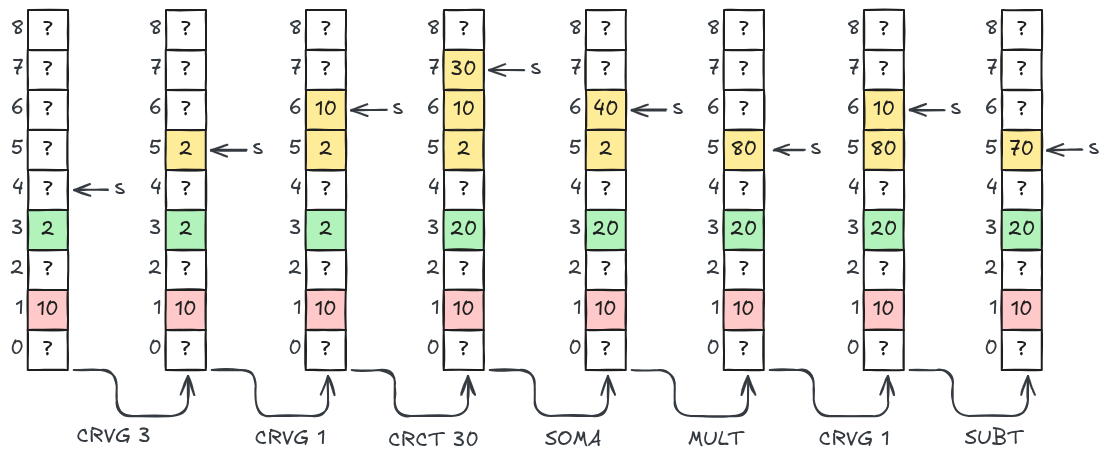
\includegraphics[width=0.8\linewidth,height=\textheight,keepaspectratio]{chapters/images/mvs-expressao.png}

}

\caption{\label{fig-expressao}Simulação das operações na pilha de
execução}

\end{figure}%

\begin{enumerate}
\def\labelenumi{\arabic{enumi}.}
\tightlist
\item
  \texttt{CRVG\ 3} carrega o valor de \texttt{B\ (2)} na pilha.
\item
  \texttt{CRVG\ 1} carrega o valor de \texttt{A\ (10)} no topo.
\item
  \texttt{CRCT\ 30} carrega a constante \texttt{30} e coloca no topo.
\item
  \texttt{SOMA} combina \texttt{10} e \texttt{30}, produzindo
  \texttt{40}.
\item
  \texttt{MULT} combina \texttt{2} e \texttt{40}, produzindo
  \texttt{80}.
\item
  \texttt{CRVG\ 1} carrega novamente o valor de \texttt{A}, isto é,
  \texttt{10} no topo.
\item
  \texttt{SUBT} calcula \texttt{80\ -\ 10}, produzindo \texttt{70}.
\end{enumerate}

O resultado corresponde à avaliação da expressão original:

\[
2 \times (10+30)-10 = 70
\]

O exemplo mostra que o compilador não precisa gerar uma instrução
específica para cada expressão completa. Ele combina operações
elementares de leitura, inserção de constantes e aritmética. A pilha
mantém os resultados intermediários até que eles sejam consumidos por
uma operação posterior.

\subsection{Tradução de comandos de
atribuição}\label{traduuxe7uxe3o-de-comandos-de-atribuiuxe7uxe3o}

Um comando de atribuição calcula o valor de uma expressão e armazena o
resultado na variável indicada à esquerda do operador de atribuição.

Considere:

\begin{Shaded}
\begin{Highlighting}[]
\NormalTok{A \textless{}{-} A + B}
\end{Highlighting}
\end{Shaded}

Suponha que os endereços das variáveis sejam \texttt{10} para \texttt{A}
e \texttt{12} para \texttt{B}. A tradução para a MVS é:

\begin{Shaded}
\begin{Highlighting}[]
\KeywordTok{CRVG}  \DecValTok{10}
\KeywordTok{CRVG}  \DecValTok{12}
\KeywordTok{SOMA}
\KeywordTok{ARZG}  \DecValTok{10}
\end{Highlighting}
\end{Shaded}

As duas primeiras instruções colocam os valores de \texttt{A} e
\texttt{B} na pilha. A instrução \texttt{SOMA} calcula o resultado e o
mantém no topo. Finalmente, \texttt{ARZG\ 10} armazena o resultado na
posição de memória associada à variável \texttt{A}.

O padrão de tradução de uma atribuição pode ser resumido em três etapas:

\begin{enumerate}
\def\labelenumi{\arabic{enumi}.}
\tightlist
\item
  Gerar as instruções necessárias para avaliar a expressão do lado
  direito.
\item
  Deixar o resultado da expressão no topo da pilha.
\item
  Utilizar \texttt{ARZG} para armazenar o resultado no endereço da
  variável do lado esquerdo.
\end{enumerate}

Essa estratégia permite traduzir atribuições com expressões de
complexidade arbitrária, desde que as expressões possam ser traduzidas
para as instruções disponíveis na MVS.

\subsection{Tradução de comandos de
seleção}\label{traduuxe7uxe3o-de-comandos-de-seleuxe7uxe3o}

O comando de seleção permite escolher entre diferentes sequências de
instruções, conforme o resultado de uma condição. Considere a estrutura:

\begin{Shaded}
\begin{Highlighting}[]
\NormalTok{se E então}
\NormalTok{    C1}
\NormalTok{senão}
\NormalTok{    C2}
\NormalTok{fimse}
\end{Highlighting}
\end{Shaded}

A tradução utiliza uma instrução condicional e uma instrução de desvio
incondicional. Primeiro, o código que avalia \texttt{E} coloca um valor
lógico no topo da pilha. Em seguida, \texttt{DSVF} desvia para o trecho
correspondente ao caso falso. Ao final do primeiro ramo, \texttt{DSVS}
evita que a execução continue indevidamente pelo segundo ramo.

O esquema geral para tradução da estrutura de seleção a linguagem
Simples está representado na Figura~\ref{fig-selecao}.

\begin{figure}

\centering{

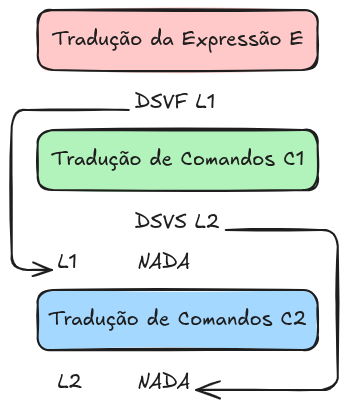
\includegraphics[width=0.4\linewidth,height=\textheight,keepaspectratio]{chapters/images/selecao.png}

}

\caption{\label{fig-selecao}Esquema de tradução da estrutura de seleção}

\end{figure}%

O rótulo \texttt{L1} identifica o início do ramo executado quando a
condição é falsa, e \texttt{L2} identifica o ponto comum após a seleção.

\subsubsection{Exemplo de seleção}\label{exemplo-de-seleuxe7uxe3o}

Considere o seguinte trecho de programa:

\begin{Shaded}
\begin{Highlighting}[]
\NormalTok{A \textless{}{-} V}
\KeywordTok{se}\NormalTok{ A}
  \KeywordTok{entao}\NormalTok{ A \textless{}{-} F}
  \KeywordTok{senao}\NormalTok{ A \textless{}{-} V}
\KeywordTok{fimse}
\end{Highlighting}
\end{Shaded}

Supondo que os valores lógicos sejam representados por \texttt{1} para
verdadeiro e \texttt{0} para falso, a tradução apresentada nos slides é:

\begin{Shaded}
\begin{Highlighting}[]
    \KeywordTok{CRCT}  \DecValTok{1}
    \KeywordTok{ARZG}  \DecValTok{0}
    \KeywordTok{CRVG}  \DecValTok{0}
    \KeywordTok{DSVF}  \FunctionTok{L1}
    \KeywordTok{CRCT}  \DecValTok{0}
    \KeywordTok{ARZG}  \DecValTok{0}
    \KeywordTok{DSVS}  \FunctionTok{L2}
\FunctionTok{L1}  \KeywordTok{NADA}
    \KeywordTok{CRCT}  \DecValTok{1}
    \KeywordTok{ARZG}  \DecValTok{0}
\FunctionTok{L2}  \KeywordTok{NADA}
\end{Highlighting}
\end{Shaded}

As primeiras instruções atribuem \texttt{1} à posição de memória
\texttt{0}, que representa a variável \texttt{A} nesse exemplo. Em
seguida, \texttt{CRVG\ 0} recupera seu valor e \texttt{DSVF\ L1}
verifica a condição.

Se \texttt{A} for falsa, a execução desvia para \texttt{L1} e atribui
\texttt{1} a \texttt{A}. Se \texttt{A} for verdadeira, a execução
prossegue, atribui \texttt{0} a \texttt{A} e salta para \texttt{L2},
evitando executar o ramo alternativo.

Esse exemplo demonstra como uma estrutura de alto nível é convertida em
instruções de carga, armazenamento e desvio. A seleção não exige uma
instrução única que represente todo o comando: seu comportamento é
obtido pela combinação de instruções elementares.

\subsection{Tradução de comandos de
repetição}\label{traduuxe7uxe3o-de-comandos-de-repetiuxe7uxe3o}

Os comandos de repetição são implementados por meio de desvios que
retornam a um ponto anterior do programa. Considere a estrutura:

\begin{Shaded}
\begin{Highlighting}[]
\NormalTok{enquanto E faca}
\NormalTok{    C}
\NormalTok{fimenquanto}
\end{Highlighting}
\end{Shaded}

A condição precisa ser avaliada antes de cada execução do corpo. Se for
verdadeira, o corpo é executado e o controle retorna ao ponto de
avaliação. Se for falsa, a execução desvia para a instrução posterior ao
laço.

O esquema geral para tradução da estrutura de seleção a linguagem
Simples está representado na Figura~\ref{fig-repeticao}.

\begin{figure}

\centering{

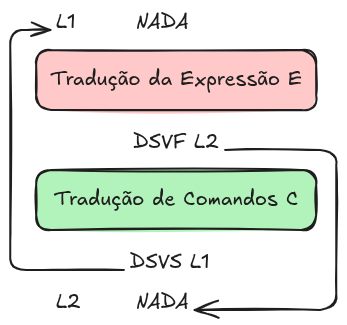
\includegraphics[width=0.4\linewidth,height=\textheight,keepaspectratio]{chapters/images/repeticao.png}

}

\caption{\label{fig-repeticao}Esquema de tradução da estrutura de
repetição}

\end{figure}%

O rótulo \texttt{L1} identifica o início do teste. O rótulo \texttt{L2}
identifica a saída do laço. A instrução \texttt{DSVS\ L1} faz com que a
condição seja avaliada novamente após a execução do corpo.

\subsubsection{Exemplo de repetição}\label{exemplo-de-repetiuxe7uxe3o}

Considere o programa:

\begin{Shaded}
\begin{Highlighting}[]
\NormalTok{x \textless{}{-} }\DecValTok{1}
\KeywordTok{enquanto}\NormalTok{ x \textless{} }\DecValTok{10} \KeywordTok{faca}
\NormalTok{    x \textless{}{-} }\DecValTok{2}\NormalTok{ * x}
\KeywordTok{fimenquanto}
\end{Highlighting}
\end{Shaded}

A tradução para a MVS é:

\begin{Shaded}
\begin{Highlighting}[]
    \KeywordTok{CRCT}  \DecValTok{1}
    \KeywordTok{ARZG}  \DecValTok{0}
\FunctionTok{L1}  \KeywordTok{NADA}
    \KeywordTok{CRVG}  \DecValTok{0}
    \KeywordTok{CRCT}  \DecValTok{10}
    \KeywordTok{CMME}
    \KeywordTok{DSVF}  \FunctionTok{L2}
    \KeywordTok{CRCT}  \DecValTok{2}
    \KeywordTok{CRVG}  \DecValTok{0}
    \KeywordTok{MULT}
    \KeywordTok{ARZG}  \DecValTok{0}
    \KeywordTok{DSVS}  \FunctionTok{L1}
\FunctionTok{L2}  \KeywordTok{NADA}
\end{Highlighting}
\end{Shaded}

As primeiras instruções atribuem \texttt{1} a \texttt{x}. Em seguida, o
programa testa a condição \texttt{x\ \textless{}\ 10}. A instrução
\texttt{CMME} produz \texttt{1} se o valor de \texttt{x} for menor que
\texttt{10} e \texttt{0} caso contrário.

Se o resultado for falso, \texttt{DSVF\ L2} encerra a repetição. Se for
verdadeiro, o programa calcula \texttt{2\ *\ x}, armazena o resultado em
\texttt{x} e retorna ao rótulo \texttt{L1}.

A sequência dos valores de \texttt{x} será:

\[
1 \rightarrow 2 \rightarrow 4 \rightarrow 8 \rightarrow 16
\]

Quando \texttt{x} passa a valer \texttt{16}, a condição
\texttt{x\ \textless{}\ 10} é falsa, e o laço termina. O exemplo ilustra
como um comando de repetição é representado por um ciclo no fluxo de
controle do código gerado.

\subsection{Tradução de comandos de entrada e
saída}\label{traduuxe7uxe3o-de-comandos-de-entrada-e-sauxedda}

A MVS oferece as instruções \texttt{LEIA} e \texttt{ESCR} para realizar
operações de entrada e saída. A primeira obtém um valor e o coloca no
topo da pilha; a segunda exibe o valor do topo e o remove.

Considere o programa:

\begin{Shaded}
\begin{Highlighting}[]
\KeywordTok{leia}\NormalTok{ A}
\KeywordTok{leia}\NormalTok{ B}
\KeywordTok{escreva}\NormalTok{ A + B}
\end{Highlighting}
\end{Shaded}

Supondo que as variáveis \texttt{A} e \texttt{B} estejam associadas às
posições \texttt{0} e \texttt{1}, respectivamente, a tradução é:

\begin{Shaded}
\begin{Highlighting}[]
    \KeywordTok{LEIA}
    \KeywordTok{ARZG}  \DecValTok{0}
    \KeywordTok{LEIA}
    \KeywordTok{ARZG}  \DecValTok{1}
    \KeywordTok{CRVG}  \DecValTok{0}
    \KeywordTok{CRVG}  \DecValTok{1}
    \KeywordTok{SOMA}
    \KeywordTok{ESCR}
\end{Highlighting}
\end{Shaded}

A primeira instrução \texttt{LEIA} recebe um valor, que é armazenado em
\texttt{M{[}0{]}} por \texttt{ARZG\ 0}. A segunda leitura é armazenada
em \texttt{M{[}1{]}}. Depois, \texttt{CRVG\ 0} e \texttt{CRVG\ 1}
colocam os dois valores na pilha, \texttt{SOMA} calcula o resultado e
\texttt{ESCR} apresenta a soma.

Esse padrão também evidencia a divisão de responsabilidades entre o
compilador e a máquina virtual. O compilador traduz os comandos para uma
sequência de instruções, enquanto a execução dessas instruções realiza
as operações de entrada, armazenamento, cálculo e saída.

\subsection{Tradução de um programa
completo}\label{traduuxe7uxe3o-de-um-programa-completo}

Para traduzir um programa completo, é necessário inicializar a máquina,
reservar espaço para as variáveis e encerrar a execução adequadamente.

As instruções de controle utilizadas são:

\begin{itemize}
\tightlist
\item
  \texttt{INPP}: inicializa a máquina, definindo \(s=-1\), \(i=1\) e
  \(d=0\).
\item
  \texttt{AMEM\ n}: reserva espaço para as variáveis globais, avançando
  o topo da pilha em \texttt{n} posições.
\item
  \texttt{FIMP}: finaliza a execução.
\end{itemize}

Considere o programa:

\begin{Shaded}
\begin{Highlighting}[]
\KeywordTok{programa}\NormalTok{ repete}
  \KeywordTok{inteiro}\NormalTok{ i j}
\KeywordTok{inicio}
\NormalTok{  i \textless{}{-} }\DecValTok{1}
  \KeywordTok{enquanto}\NormalTok{ i \textless{} }\DecValTok{10} \KeywordTok{faca}
\NormalTok{    j \textless{}{-} }\DecValTok{1}
    \KeywordTok{enquanto}\NormalTok{ j \textless{} }\DecValTok{10} \KeywordTok{faca}
      \KeywordTok{escreva}\NormalTok{ i + j}
\NormalTok{      j \textless{}{-} j + }\DecValTok{1}
    \KeywordTok{fimenquanto}
\NormalTok{    i \textless{}{-} i + }\DecValTok{1}
  \KeywordTok{fimenquanto}
\KeywordTok{fimprograma}
\end{Highlighting}
\end{Shaded}

A tradução apresentada nos slides é:

\begin{Shaded}
\begin{Highlighting}[]
    \KeywordTok{INPP}
    \KeywordTok{AMEM}  \DecValTok{2}
    \KeywordTok{CRCT}  \DecValTok{1}
    \KeywordTok{ARZG}  \DecValTok{0}
\FunctionTok{L1}  \KeywordTok{NADA}
    \KeywordTok{CRVG}  \DecValTok{0}
    \KeywordTok{CRCT}  \DecValTok{10}
    \KeywordTok{CMME}
    \KeywordTok{DSVF}  \FunctionTok{L2}
    \KeywordTok{CRCT}  \DecValTok{1}
    \KeywordTok{ARZG}  \DecValTok{1}
\FunctionTok{L3}  \KeywordTok{NADA}
    \KeywordTok{CRVG}  \DecValTok{1}
    \KeywordTok{CRCT}  \DecValTok{10}
    \KeywordTok{CMME}
    \KeywordTok{DSVF}  \FunctionTok{L4}
    \KeywordTok{CRVG}  \DecValTok{0}
    \KeywordTok{CRVG}  \DecValTok{1}
    \KeywordTok{SOMA}
    \KeywordTok{ESCR}
    \KeywordTok{CRVG}  \DecValTok{1}
    \KeywordTok{CRCT}  \DecValTok{1}
    \KeywordTok{SOMA}
    \KeywordTok{ARZG}  \DecValTok{1}
    \KeywordTok{DSVS}  \FunctionTok{L3}
\FunctionTok{L4}  \KeywordTok{NADA}
    \KeywordTok{CRVG}  \DecValTok{0}
    \KeywordTok{CRCT}  \DecValTok{1}
    \KeywordTok{SOMA}
    \KeywordTok{ARZG}  \DecValTok{0}
    \KeywordTok{DSVS}  \FunctionTok{L1}
\FunctionTok{L2}  \KeywordTok{NADA}
    \KeywordTok{FIMP}
\end{Highlighting}
\end{Shaded}

A instrução \texttt{INPP} inicializa a máquina, e \texttt{AMEM\ 2}
reserva espaço para as duas variáveis inteiras. Neste exemplo,
\texttt{i} é armazenada em \texttt{M{[}0{]}} e \texttt{j} em
\texttt{M{[}1{]}}.

O primeiro laço, identificado por \texttt{L1} e \texttt{L2}, controla os
valores de \texttt{i}. Para cada valor de \texttt{i} menor que
\texttt{10}, o programa inicializa \texttt{j} com \texttt{1} e executa o
laço interno, identificado por \texttt{L3} e \texttt{L4}.

No laço interno, o programa calcula e exibe \texttt{i\ +\ j}. Depois,
incrementa \texttt{j} e retorna a \texttt{L3} para testar novamente a
condição \texttt{j\ \textless{}\ 10}. Quando essa condição se torna
falsa, a execução sai do laço interno, incrementa \texttt{i} e retorna a
\texttt{L1}.

Quando \texttt{i\ \textless{}\ 10} deixa de ser verdadeira, a execução
prossegue para \texttt{L2} e alcança \texttt{FIMP}, encerrando o
programa.

O exemplo reúne os principais mecanismos da MVS: manipulação da pilha,
leitura e armazenamento de variáveis, operações aritméticas, comparação,
desvios condicionais e desvios incondicionais. Ele mostra como
estruturas de alto nível podem ser representadas por uma sequência de
instruções simples.

\subsection{Relação entre a máquina de Turing, a máquina virtual e o
compilador}\label{relauxe7uxe3o-entre-a-muxe1quina-de-turing-a-muxe1quina-virtual-e-o-compilador}

A máquina de Turing e a MVS são modelos abstratos de computação, mas
foram concebidos para finalidades diferentes.

A máquina de Turing é utilizada para estudar formalmente a
computabilidade e os limites dos algoritmos. Sua descrição concentra-se
nos estados, na fita, no cabeçote e na função de transição. Ela permite
investigar se um problema admite um procedimento algorítmico,
independentemente de detalhes de implementação.

A MVS, por sua vez, foi projetada para facilitar o estudo da execução de
programas compilados. Sua organização em memória de programa, pilha de
dados e registradores torna explícitos os mecanismos utilizados para
avaliar expressões e controlar o fluxo de execução.

O compilador conecta a linguagem de alto nível à representação
executável pela máquina virtual. Ele traduz as construções da
linguagem-fonte em sequências de instruções da MVS, procurando preservar
o significado do programa original. A máquina virtual executa o código
gerado segundo as regras definidas para cada instrução.

É importante distinguir a tradução da execução. O compilador produz uma
representação do programa; o interpretador ou simulador da MVS executa
essa representação. Em uma implementação didática, ambos podem ser
desenvolvidos como programas separados, o que facilita testar a correção
da tradução e a semântica das instruções.

A MVS não é necessariamente uma máquina virtual de um produto comercial
nem depende de um sistema operacional específico. Trata-se de uma
arquitetura didática definida para tornar visíveis os princípios
fundamentais da geração e execução de código.

\subsection{Simulador da Máquina Virtual
Simples}\label{simulador-da-muxe1quina-virtual-simples}

O simulador da Máquina Virtual Simples (MVS) em sequência permite
executar programas e acompanhar como as instruções modificam a pilha, os
registradores e o fluxo de execução. A ferramenta oferece um editor de
código, visualização da pilha de operandos, indicação da instrução atual
e um terminal para entrada e saída de dados.

As instruções sem rótulo devem começar com uma tabulação. Os rótulos são
escritos no início da linha, sem dois-pontos, seguidos de uma tabulação
e da instrução associada. Para definir um rótulo sem operação, utilize
\texttt{NADA}.

Exemplo de programa que soma dois valores:

\begin{Shaded}
\begin{Highlighting}[]
    \KeywordTok{INPP}
    \KeywordTok{CRCT}    \DecValTok{10}
    \KeywordTok{CRCT}    \DecValTok{20}
    \KeywordTok{SOMA}
    \KeywordTok{ESCR}
    \KeywordTok{FIMP}
\end{Highlighting}
\end{Shaded}

O programa coloca os valores 10 e 20 na pilha, soma os operandos,
apresenta o resultado no terminal e encerra a execução.

Execute o programa passo a passo e observe as alterações na pilha e nos
registradores de controle. O registrador \texttt{s} indica a próxima
posição livre da pilha, enquanto \texttt{i} indica a próxima instrução a
ser executada.

No exemplo, \texttt{CRCT} insere valores na pilha, \texttt{SOMA}
substitui os dois operandos pelo resultado 30 e \texttt{ESCR} apresenta
esse resultado no terminal.

Modifique o programa inicial para experimentar operações aritméticas,
entrada de dados com \texttt{LEIA}, desvios condicionais e laços de
repetição. Antes de executar cada instrução, tente prever seu efeito e
compare sua previsão com o comportamento observado. Assim, será possível
compreender melhor a semântica das instruções e o funcionamento da MVS.

\begin{figure}[H]
\centering
\fbox{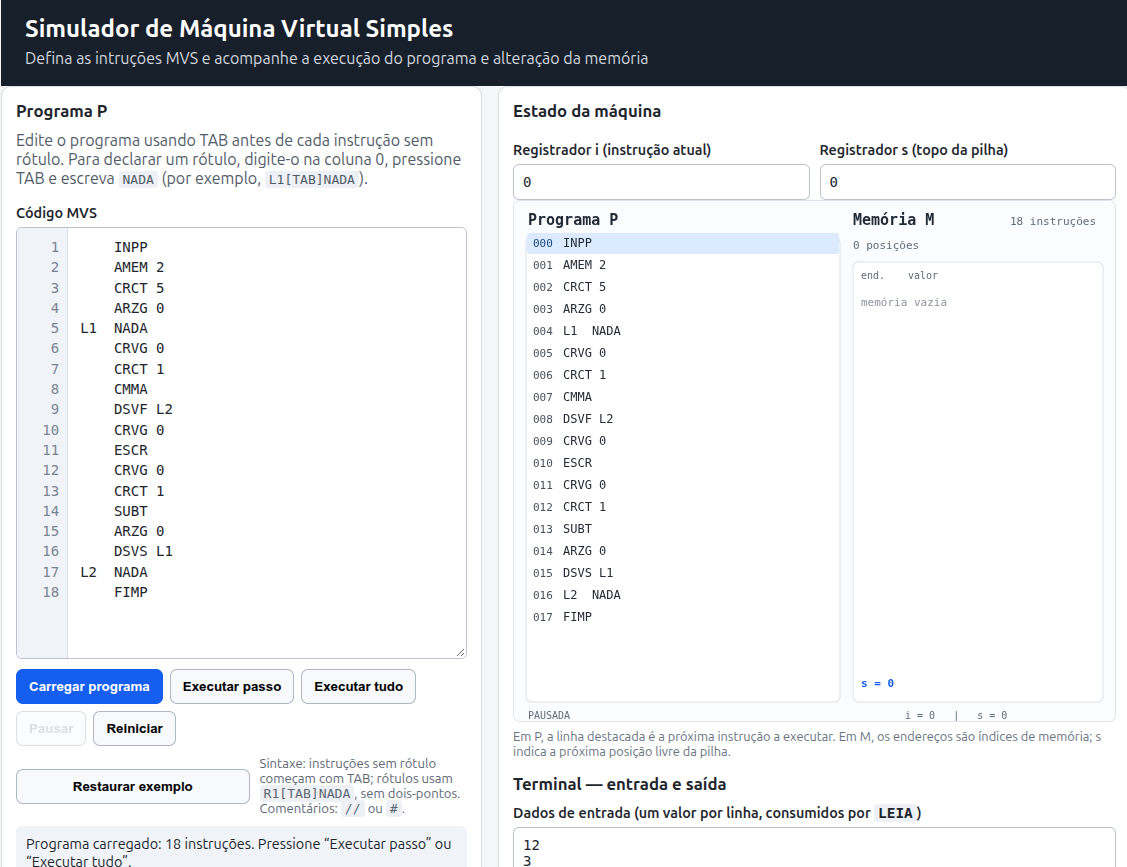
\includegraphics[width=0.6\textwidth]{chapters/images/printscreen/mvs.png}}
\caption{Visualização da aplicação interativa}
\end{figure}
\begin{tcolorbox}[enhanced jigsaw, title=Acesso Interativo]
Acesse a simulação em:\par\smallskip
\small\url{https://luizedsilva.github.io/Livro-LTC/p5js/mvs/}
\begin{center}
\includegraphics[width=3cm]{chapters/images/qrcode/mvs.png}\end{center}
\end{tcolorbox}

\subsection{Considerações finais}\label{considerauxe7uxf5es-finais-1}

A passagem de uma linguagem de alto nível para uma máquina virtual
permite compreender como as construções de um programa são transformadas
em operações elementares. Expressões são traduzidas em sequências que
manipulam a pilha; atribuições combinam avaliação e armazenamento;
seleções e repetições são implementadas por desvios; e comandos de
entrada e saída utilizam instruções específicas.

A MVS fornece um ambiente reduzido no qual esses mecanismos podem ser
estudados sem a complexidade de uma arquitetura real. Ao mesmo tempo, a
descrição de sua execução por meio de memória, registradores e
instruções reforça uma ideia central da teoria da computação: um
programa pode ser entendido como uma sequência de transformações de
estado, cada uma determinada pelas regras de execução da máquina.

Dessa forma, o estudo da MVS complementa o estudo da máquina de Turing.
Enquanto a máquina de Turing oferece uma base para compreender o que
pode ser computado, a máquina virtual ajuda a compreender como um
compilador representa e prepara um programa para execução.

\bookmarksetup{startatroot}

\chapter{A Análise Semântica e a Geração de
Código}\label{a-anuxe1lise-semuxe2ntica-e-a-gerauxe7uxe3o-de-cuxf3digo}

\begin{center}
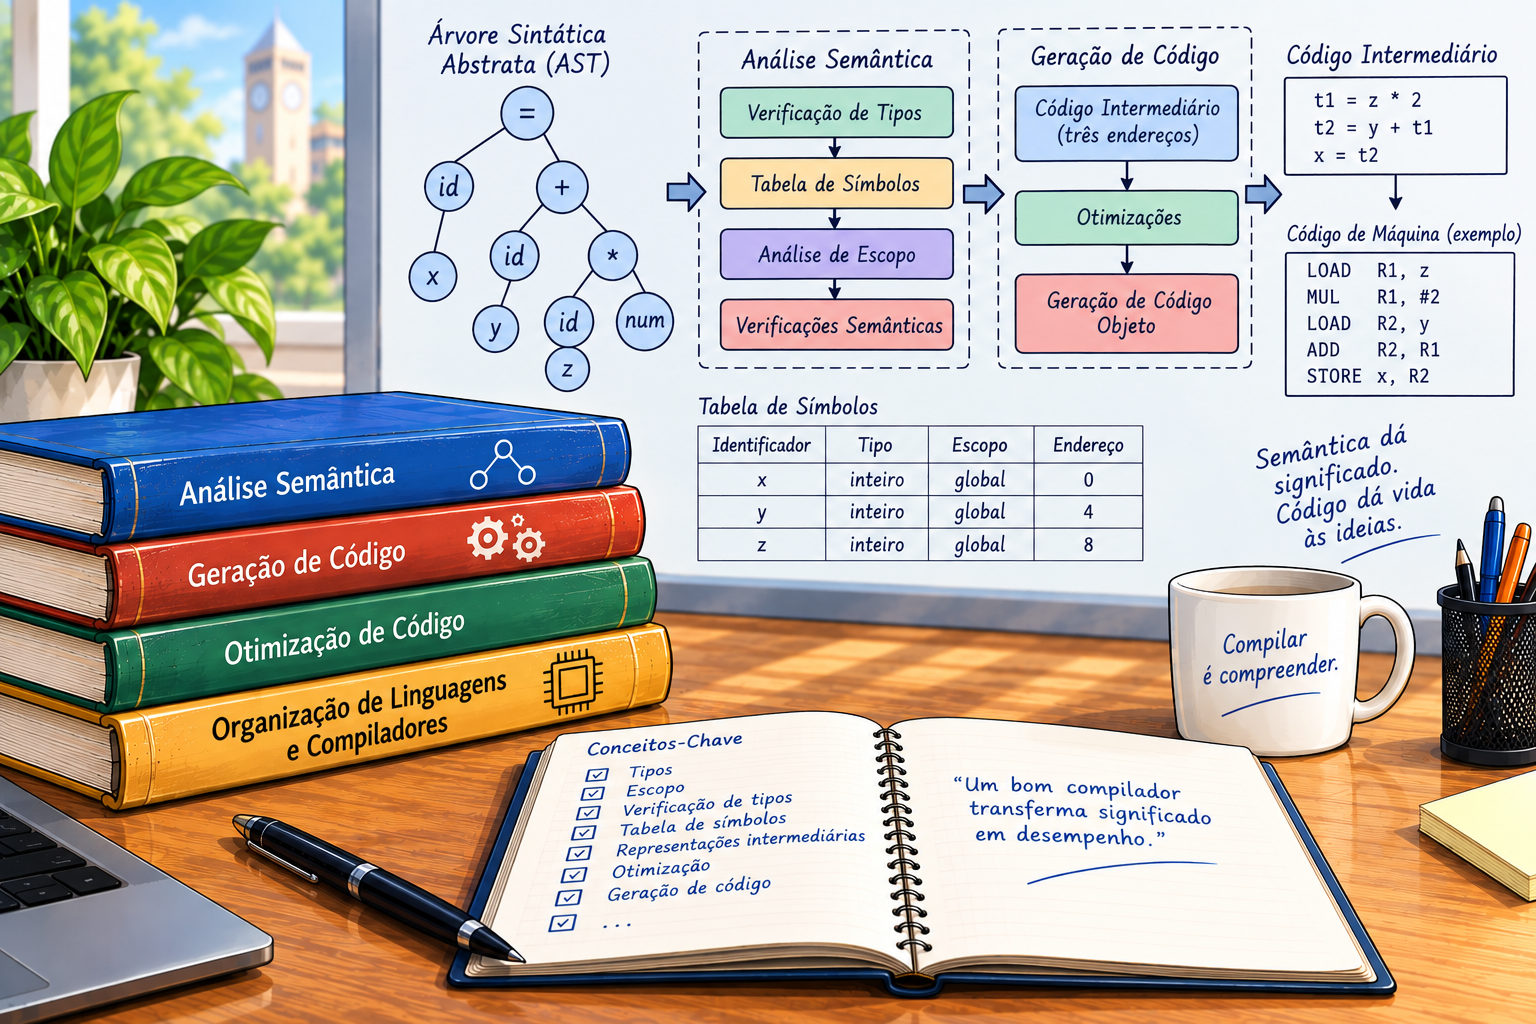
\includegraphics[width=0.7\linewidth,height=\textheight,keepaspectratio]{chapters/images/semantico.png}
\end{center}

A análise semântica e a geração de código são etapas fundamentais do
processo de compilação. Enquanto a análise léxica identifica os
elementos que compõem o programa e a análise sintática verifica se esses
elementos estão organizados de acordo com a gramática da linguagem, a
análise semântica verifica se o programa possui significado válido
segundo as regras da linguagem. Em seguida, a geração de código
transforma a estrutura analisada em uma representação adequada para
execução ou para uma etapa posterior do processo de compilação.

Essas etapas estabelecem a ligação entre a estrutura formal de um
programa e seu comportamento durante a execução. Para compreender essa
relação, é necessário considerar não apenas a organização dos comandos,
mas também o significado das variáveis, os tipos dos dados, as
declarações e as operações realizadas.

Neste capítulo, estudaremos como o compilador utiliza as informações
produzidas pelas etapas anteriores para verificar a consistência do
programa e transformá-lo em código. Também veremos por que uma
representação intermediária facilita a separação entre as
características da linguagem de origem e as particularidades da máquina
ou do ambiente de execução de destino.

\section{Da análise sintática à análise
semântica}\label{da-anuxe1lise-sintuxe1tica-uxe0-anuxe1lise-semuxe2ntica}

A análise sintática determina se um programa pode ser reconhecido pela
gramática da linguagem. Seu resultado é, geralmente, uma árvore
sintática ou uma árvore sintática abstrata (Abstract Syntax Tree ---
AST), que representa a organização hierárquica dos elementos do
programa. Entretanto, reconhecer uma estrutura sintática válida não é
suficiente para garantir que o programa esteja correto.

Considere o seguinte trecho de uma linguagem de programação hipotética:

\begin{Shaded}
\begin{Highlighting}[]
\KeywordTok{inteiro}\NormalTok{ idade}
\NormalTok{idade \textless{}{-} }\DecValTok{20}
\end{Highlighting}
\end{Shaded}

Supondo que a linguagem permita a declaração de variáveis inteiras e
comandos de atribuição, esse programa apresenta uma estrutura sintática
válida. A declaração introduz a variável \texttt{idade}, e a atribuição
associa a ela o valor \texttt{20}.

Agora, considere o seguinte trecho:

\begin{Shaded}
\begin{Highlighting}[]
\NormalTok{idade \textless{}{-} }\DecValTok{20}
\end{Highlighting}
\end{Shaded}

Esse segundo trecho também pode ser sintaticamente válido. Entretanto,
se a linguagem exigir que uma variável seja declarada antes de sua
utilização e não existir nenhuma declaração anterior de \texttt{idade},
o programa apresenta um erro semântico.

A diferença entre os dois casos evidencia que a análise sintática e a
análise semântica verificam propriedades distintas. A primeira examina a
organização dos símbolos de acordo com as regras gramaticais; a segunda
verifica se essa organização faz algum sentido dentro do contexto do
programa usando a linguagem de programação.

Em um compilador, essa etapa normalmente depende de informações que não
podem ser verificadas apenas pela gramática, como as declarações
existentes, os tipos das expressões e as regras de visibilidade dos
identificadores. Para realizar essas verificações, o compilador mantém
estruturas auxiliares, como a tabela de símbolos e a pilha semântica, e
percorre a árvore sintática para examinar as construções do programa.

A análise semântica não substitui a análise sintática. Ao contrário, ela
utiliza seus resultados para realizar verificações de natureza
diferente. Em geral, um compilador só inicia a análise semântica sobre
uma unidade sintática quando dispõe de uma estrutura suficientemente
válida para examiná-la.

\subsection{O papel da análise
semântica}\label{o-papel-da-anuxe1lise-semuxe2ntica}

A análise semântica verifica se as construções sintaticamente válidas
obedecem às regras que definem seu significado na linguagem de
programação. Seu objetivo é identificar inconsistências que poderiam
comprometer a tradução ou a execução do programa.

As verificações realizadas dependem das características da linguagem.
Entre as mais comuns, destacam-se:

\begin{itemize}
\tightlist
\item
  Declaração de identificadores: verificar se variáveis, funções e
  outros identificadores utilizados no programa foram declarados
  conforme as regras da linguagem.
\item
  Escopo e visibilidade: determinar em quais regiões do programa cada
  identificador pode ser utilizado.
\item
  Verificação de tipos: conferir se os tipos dos operandos são
  compatíveis com as operações realizadas.
\item
  Compatibilidade de atribuição: verificar se o valor de uma expressão
  pode ser atribuído à variável de destino.
\item
  Uso correto de operações e chamadas: conferir a quantidade e os tipos
  dos argumentos de uma função, quando aplicável, bem como as restrições
  impostas aos operadores.
\item
  Consistência das estruturas de controle: verificar condições e outras
  restrições semânticas associadas a comandos condicionais, laços e
  retornos de funções.
\end{itemize}

Considere o exemplo:

\begin{Shaded}
\begin{Highlighting}[]
\KeywordTok{inteiro}\NormalTok{ x}
\KeywordTok{logico}\NormalTok{ y}

\NormalTok{x \textless{}{-} }\DecValTok{10}
\NormalTok{y \textless{}{-} V}
\NormalTok{y \textless{}{-} x + y}
\end{Highlighting}
\end{Shaded}

Nesse programa, a análise semântica identifica que \texttt{x} possui
tipo inteiro e \texttt{y} possui tipo lógico. A expressão
\texttt{x\ +\ y} combina um operando inteiro com um operando lógico. Se
a linguagem permitir essa operação, o compilador deverá determinar como
os tipos são tratados, por exemplo, por meio da conversão do valor
lógico para inteiro. A atribuição do resultado a \texttt{y} será então
verificada de acordo com as regras de compatibilidade da linguagem.

Essas regras não são universais. Algumas linguagens permitem conversões
implícitas entre determinados tipos, enquanto outras exigem conversões
explícitas. Da mesma forma, certas linguagens são mais permissivas
quanto à utilização de valores em expressões, enquanto outras impõem
verificações mais rigorosas.

A análise semântica também pode exigir informações sobre declarações que
aparecem em outras partes do programa. Por exemplo, ao encontrar uma
chamada de função, o compilador pode precisar consultar a tabela de
símbolos para verificar sua existência, seus parâmetros e seu tipo de
retorno.

A tabela de símbolos é uma estrutura de dados utilizada para armazenar
informações sobre os identificadores do programa. Dependendo da
linguagem e da implementação do compilador, ela pode registrar o nome de
cada identificador, seu tipo, sua categoria, seu escopo, seus parâmetros
e outras propriedades relevantes. Essas informações são consultadas
durante a análise semântica e podem ser reutilizadas na geração de
código.

Ao final dessa etapa, o compilador dispõe de uma estrutura sintática
enriquecida com informações semânticas. Isso permite que a geração de
código utilize os tipos, as declarações e as características das
operações para produzir uma representação coerente com o significado do
programa original.

É importante observar que a análise semântica não garante a ausência de
todos os erros possíveis. Ela verifica as propriedades que podem ser
determinadas pelas regras da linguagem e pelas informações disponíveis
durante a compilação. Erros relacionados a valores de entrada, condições
de execução ou outros comportamentos dependentes do ambiente podem
continuar ocorrendo durante a execução.

\subsection{Da estrutura sintática à
execução}\label{da-estrutura-sintuxe1tica-uxe0-execuuxe7uxe3o}

Depois de analisar sintaticamente e semanticamente um programa, o
compilador precisa transformá-lo em uma forma que possa ser executada
por um processador ou por um ambiente de execução. Essa transformação é
conhecida como geração de código e pode envolver várias etapas
intermediárias.

Para compreender esse processo, considere o seguinte programa
hipotético:

\begin{Shaded}
\begin{Highlighting}[]
\KeywordTok{inteiro}\NormalTok{ a b resultado}

\NormalTok{a \textless{}{-} }\DecValTok{10}
\NormalTok{b \textless{}{-} }\DecValTok{20}
\NormalTok{resultado \textless{}{-} a + b}
\end{Highlighting}
\end{Shaded}

A análise sintática identifica as declarações, as atribuições e a
expressão aritmética, organizando esses elementos em uma árvore
sintática abstrata. A análise semântica verifica se as variáveis foram
declaradas, se seus tipos são compatíveis e se a operação de adição é
válida.

Essas etapas permitem compreender o significado do programa, mas ainda
não definem diretamente como suas operações serão realizadas por uma
máquina. É necessário traduzir as construções da linguagem de origem
para instruções que representem as operações correspondentes.

Uma possível representação intermediária na forma de triplas do trecho
do programa poderia ser:

\begin{longtable*}[]{|
  >{\raggedright\arraybackslash}p{(\linewidth - 8\tabcolsep - 5\arrayrulewidth) * \real{0.2500}}|
  >{\raggedright\arraybackslash}p{(\linewidth - 8\tabcolsep - 5\arrayrulewidth) * \real{0.2500}}|
  >{\raggedright\arraybackslash}p{(\linewidth - 8\tabcolsep - 5\arrayrulewidth) * \real{0.2500}}|
  >{\raggedright\arraybackslash}p{(\linewidth - 8\tabcolsep - 5\arrayrulewidth) * \real{0.2500}}|}
\toprule\noalign{}
\begin{minipage}[b]{\linewidth}\smallskip
\raggedright
Índice
\end{minipage} & \begin{minipage}[b]{\linewidth}\raggedright
Operador (\texttt{op})
\end{minipage} & \begin{minipage}[b]{\linewidth}\raggedright
Argumento 1 (\texttt{arg1})
\end{minipage} & \begin{minipage}[b]{\linewidth}\raggedright
Argumento 2 (\texttt{arg2})
\end{minipage} \\
\midrule\noalign{}
\endhead
\bottomrule\noalign{}
\endlastfoot
\textbf{(0)} & \texttt{\textless{}-} & \texttt{10} & \texttt{a} \\
\midrule
\textbf{(1)} & \texttt{\textless{}-} & \texttt{20} & \texttt{b} \\
\midrule
\textbf{(2)} & \texttt{+} & \texttt{a} & \texttt{b} \\
\midrule
\textbf{(3)} & \texttt{\textless{}-} & \texttt{(2)} &
\texttt{resultado} \\
\end{longtable*}

Nessa representação, a expressão aritmética é calculada e seu resultado
é armazenado em uma variável temporária, identificada por \textbf{(2)}.
O valor calculado é posteriormente atribuído à variável
\texttt{resultado}.

A representação intermediária não precisa reproduzir exatamente a
sintaxe da linguagem original. Seu propósito é expressar as operações do
programa de maneira mais simples e adequada às transformações realizadas
pelo compilador.

A partir dessa representação, pode-se gerar código para diferentes
destinos. Em uma máquina virtual didática, por exemplo, as operações
poderiam ser traduzidas para instruções de carregamento de valores,
realização de operações aritméticas e armazenamento de resultados. Em um
processador real, o compilador poderia gerar instruções de máquina,
incluindo operações sobre registradores e posições de memória.

O processo pode ser sintetizado da seguinte maneira:

\begin{figure}

\centering{

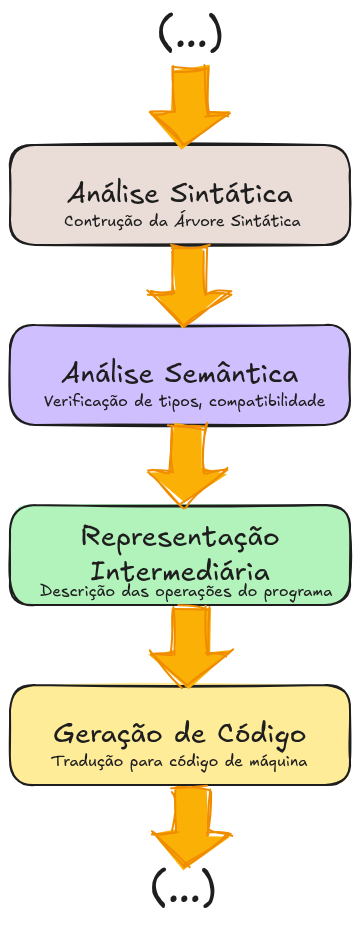
\includegraphics[width=0.3\linewidth,height=\textheight,keepaspectratio]{chapters/images/semantico-geracao.png}

}

\caption{\label{fig-semantico}Parte do processo de geração de código}

\end{figure}%

A Figura~\ref{fig-semantico} apresenta uma visão simplificada do fluxo
de compilação. Implementações reais podem incluir etapas adicionais,
como otimização, análise de fluxo de dados, alocação de registradores e
geração de código específico para a arquitetura de destino.

Também é importante distinguir a geração de código da execução. Em um
processo de compilação tradicional, o compilador produz um programa
executável ou um código intermediário que será executado posteriormente.
Em outras implementações, o código pode ser interpretado ou compilado
durante a própria execução. Essas diferenças dependem da arquitetura da
linguagem e do ambiente de execução.

\subsection{A necessidade de uma representação
intermediária}\label{a-necessidade-de-uma-representauxe7uxe3o-intermediuxe1ria}

Uma questão importante no desenvolvimento de compiladores é como separar
as características da linguagem de origem das particularidades da
plataforma de destino. Uma tradução direta entre cada linguagem de
programação e cada arquitetura pode exigir a implementação de muitos
tradutores diferentes.

Suponha que um compilador precise traduzir programas escritos em duas
linguagens de origem para três arquiteturas de destino. Se cada
linguagem for traduzida diretamente para cada arquitetura, serão
necessárias, potencialmente, seis combinações de tradutores, conforme
ilustrado na Figura~\ref{fig-representacao1}.

\begin{figure}

\centering{

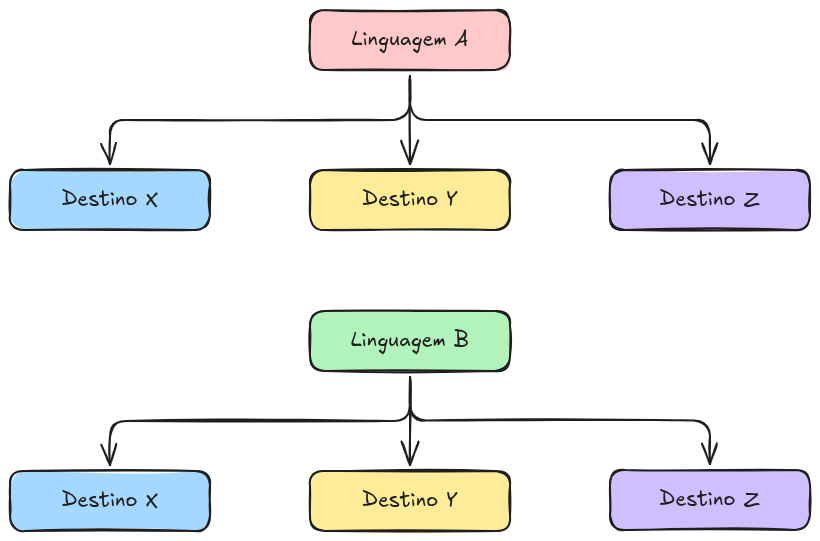
\includegraphics[width=0.8\linewidth,height=\textheight,keepaspectratio]{chapters/images/representacao1.png}

}

\caption{\label{fig-representacao1}Sem representação intermediária}

\end{figure}%

Com uma representação intermediária comum, cada linguagem pode ser
traduzida para essa representação, e cada arquitetura pode receber um
gerador específico capaz de convertê-la em seu próprio código. Nesse
cenário simplificado, seriam necessários dois tradutores para a
representação intermediária e três geradores de código, totalizando
cinco componentes de tradução.

Com representação intermediária, os tradutores e os geradores podem ser
desenvolvidos de forma independente, conforme ilustrado na
Figura~\ref{fig-representacao2}.

\begin{figure}

\centering{

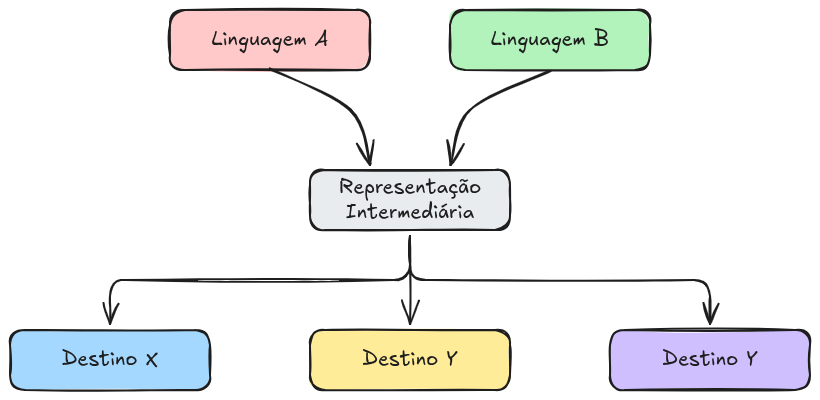
\includegraphics[width=0.8\linewidth,height=\textheight,keepaspectratio]{chapters/images/representacao2.png}

}

\caption{\label{fig-representacao2}Com representação intermediária}

\end{figure}%

O número de combinações cresce com a quantidade de linguagens e
destinos. Por exemplo, 3 linguagens e 5 destinos totalizam 15
componentes de tradução sem representação intermediária e 8 componentes
com representação intermediária.

Essa separação facilita a manutenção e a expansão de um compilador. Para
adicionar uma nova linguagem de origem, pode-se implementar um tradutor
para a representação intermediária existente. Para oferecer suporte a
uma nova arquitetura, pode-se implementar um gerador de código
correspondente, desde que ele seja compatível com essa representação.

Além disso, a representação intermediária favorece a otimização. Como
ela expressa as operações do programa de maneira independente de muitos
detalhes da linguagem original, o compilador pode identificar
oportunidades para simplificar expressões, eliminar cálculos
desnecessários e melhorar a utilização dos recursos disponíveis.

Existem diferentes formas de representação intermediária. Entre elas,
destacam-se:

\begin{itemize}
\tightlist
\item
  Árvore sintática abstrata: representa a estrutura essencial do
  programa, omitindo detalhes sintáticos desnecessários para as etapas
  posteriores.
\item
  Código de três endereços: representa operações simples, geralmente com
  um resultado e até dois operandos, utilizando variáveis temporárias
  quando necessário.
\item
  Código para uma máquina virtual: utiliza instruções de uma máquina
  abstrata, que podem ser executadas por um interpretador ou traduzidas
  posteriormente para instruções de uma arquitetura real.
\end{itemize}

Essas representações não são necessariamente alternativas excludentes.
Um compilador pode utilizar uma árvore sintática abstrata, convertê-la
em código de três endereços, aplicar otimizações e, posteriormente,
produzir instruções para uma máquina virtual ou para um processador
específico.

Neste livro, utilizaremos uma abordagem gradual para estudar essas
transformações. A análise semântica permitirá compreender como o
compilador valida as construções de um programa, que pode ser feito
através de uma representação da árvore sintátia, por exemplo. Em
seguida, a geração de código para a Máquina Virtual Simples (MVS)
permitirá relacionar cada operação do programa às instruções executadas
pela máquina abstrata.

Dessa forma, será possível acompanhar o percurso completo de um
programa: da estrutura sintática construída pelo analisador até o código
gerado e seu comportamento durante a execução. Essa perspectiva integra
os conceitos teóricos de compilação à observação prática dos algoritmos
e das estruturas utilizadas em sua implementação.

\section{Tradução dirigida por
sintaxe}\label{traduuxe7uxe3o-dirigida-por-sintaxe}

A tradução dirigida por sintaxe é uma técnica utilizada na construção de
compiladores na qual a tradução de um programa é associada às regras
gramaticais empregadas para reconhecê-lo. A ideia central consiste em
aproveitar a estrutura sintática identificada pelo analisador para
calcular informações semânticas ou produzir código correspondente às
construções reconhecidas.

Durante a análise sintática, o compilador identifica as produções
utilizadas para reconhecer o programa. Na tradução dirigida por sintaxe,
cada produção pode ser complementada por regras semânticas ou ações que
determinam o que deve ser realizado quando essa produção é aplicada.

Essas ações podem ter diferentes objetivos. Podem calcular o valor de
uma expressão, verificar a compatibilidade entre tipos, registrar
informações na tabela de símbolos ou produzir instruções para uma
máquina virtual. Assim, a tradução deixa de ser uma atividade
completamente separada do reconhecimento sintático e passa a utilizar
diretamente a estrutura gramatical do programa.

Considere a seguinte produção de uma gramática para expressões
aritméticas:

\[ E \rightarrow E_1 + T \]

Nessa produção, \textbackslash(E\textbackslash) representa a expressão
reconhecida, enquanto \textbackslash(E\_1\textbackslash) e
\textbackslash(T\textbackslash) representam seus componentes. Os índices
são utilizados apenas para distinguir ocorrências do mesmo símbolo
gramatical.

Podemos associar à produção uma regra semântica que constrói a
representação pós-fixada da expressão:

\[ E.code = E_1.code \mathbin{\\|} T.code \mathbin{\\|} \text{"+"} \]

O operador \texttt{\textbar{}} representa a concatenação de cadeias de
caracteres. A regra estabelece que a representação da expressão
resultante é formada pela concatenação do código de \(E_1\), do código
de \(T\) e do operador de adição.

Por exemplo, para a expressão:

\begin{Shaded}
\begin{Highlighting}[]
\DecValTok{3}\NormalTok{ + }\DecValTok{4}
\end{Highlighting}
\end{Shaded}

a tradução pós-fixada produz:

\begin{Shaded}
\begin{Highlighting}[]
\DecValTok{3} \DecValTok{4} \OperatorTok{+}
\end{Highlighting}
\end{Shaded}

Essa representação coloca o operador depois dos operandos. Sua avaliação
pode ser realizada por uma máquina baseada em pilha: os valores
\texttt{3} e \texttt{4} são empilhados e, quando o operador \texttt{+} é
encontrado, os dois valores são removidos da pilha, somados e
substituídos pelo resultado.

O exemplo ilustra como uma regra gramatical pode determinar a construção
de uma representação alternativa da expressão. A mesma ideia pode ser
utilizada para produzir código de três endereços, instruções de uma
máquina virtual ou outras formas de representação intermediária.

\subsection{Definições dirigidas por sintaxe e esquemas de
tradução}\label{definiuxe7uxf5es-dirigidas-por-sintaxe-e-esquemas-de-traduuxe7uxe3o}

Existem duas formas relacionadas de especificar a tradução associada a
uma gramática: as definições dirigidas por sintaxe e os esquemas de
tradução.

Uma definição dirigida por sintaxe (DDS) associa atributos aos símbolos
da gramática e estabelece regras semânticas para calcular seus valores.
Essa abordagem descreve o que deve ser calculado a partir da estrutura
sintática, sem exigir que a especificação esteja vinculada a uma
implementação particular.

Um esquema de tradução dirigida por sintaxe associa ações executáveis às
produções gramaticais. Essas ações podem ser executadas pelo analisador
durante o reconhecimento do programa e permitem implementar diretamente
os cálculos semânticos ou a emissão de instruções.

Considere novamente a produção:

\[ E \rightarrow E_1 + T \]

Uma definição dirigida por sintaxe pode especificar a construção do
código pós-fixado por meio da regra:

\[ E.code = E_1.code \mathbin{\\|} T.code \mathbin{\\|} \text{"+"} \]

Já um esquema de tradução pode executar uma ação que imprime o operador
quando a produção é reconhecida, desde que os códigos dos operandos já
tenham sido produzidos na ordem apropriada.

Por exemplo, em uma gramática adequada à análise ascendente, a ação pode
ser escrita conceitualmente como:

\begin{verbatim}
E : E1 '+' T
    { printf("+"); }
\end{verbatim}

Nesse exemplo, a ação imprime o operador. Para obter a tradução
completa, as produções correspondentes aos operandos também precisam
produzir suas representações. A posição da ação em relação aos símbolos
da produção determina quando ela será executada.

A distinção é importante: a definição dirigida por sintaxe descreve as
relações entre atributos, enquanto o esquema de tradução especifica
ações que podem ser executadas durante a análise. Na prática, as duas
abordagens podem ser utilizadas em conjunto, conforme os requisitos do
compilador.

\section{Atributos sintetizados e
herdados}\label{atributos-sintetizados-e-herdados}

Para formalizar a tradução dirigida por sintaxe, associamos atributos
aos símbolos da gramática. Um atributo representa uma informação
relacionada a uma ocorrência de um símbolo durante a análise do
programa.

Se \(X\) é um símbolo gramatical e \(a\) é um de seus atributos,
representamos esse atributo por \(X.a\). Por exemplo, \(E.val\) pode
representar o valor de uma expressão, enquanto \(E.code\) pode armazenar
sua representação em código.

Os atributos são classificados em duas categorias principais:
sintetizados e herdados.

Atributos sintetizados. Seu valor é calculado a partir dos atributos dos
símbolos que aparecem abaixo do nó correspondente na árvore sintática,
isto é, de seus filhos. As informações fluem, portanto, das partes
componentes para a construção que as reúne.

Considere a produção:

\[ E \rightarrow E_1 + T \]

Podemos definir:

\[ E.val = E_1.val + T.val \]

O valor da expressão \(E\) é calculado a partir dos valores de seus
componentes. Esse é um atributo sintetizado.

Atributos herdados. Seu valor é determinado a partir de informações
associadas ao contexto em que o símbolo aparece, como atributos de seu
pai ou de seus irmãos na árvore sintática. As informações podem fluir de
um contexto mais amplo para uma parte específica da construção.

Por exemplo, em uma declaração de variáveis, o tipo declarado pode ser
propagado para uma lista de identificadores. O atributo que representa
esse tipo pode ser herdado pelos símbolos que representam cada
identificador, permitindo que o compilador registre corretamente suas
informações na tabela de símbolos.

A distinção pode ser resumida da seguinte forma:

\begin{longtable*}[]{|
  >{\raggedright\arraybackslash}p{(\linewidth - 6\tabcolsep - 4\arrayrulewidth) * \real{0.1905}}|
  >{\raggedright\arraybackslash}p{(\linewidth - 6\tabcolsep - 4\arrayrulewidth) * \real{0.4381}}|
  >{\raggedright\arraybackslash}p{(\linewidth - 6\tabcolsep - 4\arrayrulewidth) * \real{0.3714}}|}
\toprule\noalign{}
\begin{minipage}[b]{\linewidth}\smallskip
\raggedright
Característica
\end{minipage} & \begin{minipage}[b]{\linewidth}\raggedright
Sintetizado
\end{minipage} & \begin{minipage}[b]{\linewidth}\raggedright
Herdado
\end{minipage} \\
\midrule\noalign{}
\endhead
\bottomrule\noalign{}
\endlastfoot
Origem da informação & Principalmente os filhos & Contexto, pai ou
irmãos \\
\midrule
Direção conceitual & De baixo para cima & Do contexto para o símbolo \\
\midrule
Exemplo & Valor de uma expressão & Tipo associado a uma lista de
variáveis \\
\midrule
Uso frequente & Avaliação de expressões e construção de código &
Propagação de tipos, escopo e contexto \\
\end{longtable*}

Uma definição dirigida por sintaxe pode utilizar atributos sintetizados,
herdados ou ambos. A escolha depende da informação que precisa ser
calculada e da forma como ela está disponível durante a análise.

\section{Definição dirigida por sintaxe para uma
calculadora}\label{definiuxe7uxe3o-dirigida-por-sintaxe-para-uma-calculadora}

Considere uma gramática simplificada para avaliar expressões
aritméticas, formada por números inteiros, adição e multiplicação:

\[
\begin{aligned} 
L &\rightarrow E\ \backslash n\\
E &\rightarrow E_1 + E_2\\
E &\rightarrow E_1 * E_2\\ 
E &\rightarrow \textit{num} 
\end{aligned} 
\]

O símbolo \(L\) representa uma linha de entrada, \(E\) representa uma
expressão e \(\textit{num}\) representa um número reconhecido pelo
analisador léxico. O atributo \(\textit{num.lexval}\) corresponde ao
valor numérico associado ao token.

Podemos definir um atributo sintetizado
\textbackslash(val\textbackslash) para os símbolos
\textbackslash(L\textbackslash) e \textbackslash(E\textbackslash),
conforme as seguintes regras semânticas.

\begin{longtable*}[]{|
  >{\raggedright\arraybackslash}p{(\linewidth - 4\tabcolsep - 3\arrayrulewidth) * \real{0.6027}}|
  >{\raggedright\arraybackslash}p{(\linewidth - 4\tabcolsep - 3\arrayrulewidth) * \real{0.3973}}|}
\toprule\noalign{}
\begin{minipage}[b]{\linewidth}\smallskip
\raggedright
Produção
\end{minipage} & \begin{minipage}[b]{\linewidth}\raggedright
Regra semântica
\end{minipage} \\
\midrule\noalign{}
\endhead
\bottomrule\noalign{}
\endlastfoot
\(L \rightarrow E\ \backslash n\) & \(L.val = E.val\) \\
\midrule
\(E \rightarrow E_1 + E_2\) & \(E.val = E_1.val + E_2.val\) \\
\midrule
\(E \rightarrow E_1 * E_2\) & \(E.val = E_1.val * E_2.val\) \\
\midrule
\(E \rightarrow \textit{num}\) & \(E.val = \textit{num.lexval}\) \\
\end{longtable*}

A primeira regra transfere o valor da expressão para a linha
reconhecida. A segunda e a terceira calculam os resultados das operações
aritméticas. A última associa à expressão o valor do número reconhecido
pelo analisador léxico.

Considere a expressão:

\begin{verbatim}
3 + 4 * 5
\end{verbatim}

Supondo que a gramática atribua precedência maior à multiplicação do que
à adição, a árvore sintática terá a multiplicação como subexpressão da
adição. Os atributos sintetizados serão calculados das folhas em direção
à raiz:

\(E.val = 23\)

3 + 20

3

Valor: 3

+

Adição

\(E.val = 20\)

4 × 5

A multiplicação é avaliada antes da adição, e o resultado é sintetizado
até a raiz.

O resultado da multiplicação é \(4 \times 5 = 20\). Em seguida, a adição
calcula \(3 + 20 = 23\). O atributo da raiz contém o valor final da
expressão.

Esse exemplo mostra que a definição dirigida por sintaxe permite
descrever a avaliação de expressões diretamente a partir da estrutura
gramatical. A mesma técnica pode ser empregada para construir código,
verificar tipos ou calcular outras propriedades necessárias à
compilação.

\section{Esquemas de tradução dirigida por
sintaxe}\label{esquemas-de-traduuxe7uxe3o-dirigida-por-sintaxe}

Em um esquema de tradução, as ações semânticas são associadas às
produções gramaticais e executadas nos pontos determinados por sua
posição. Uma ação pode calcular um atributo, consultar a tabela de
símbolos ou emitir instruções para a máquina de destino.

Para a calculadora anterior, um esquema de tradução pode ser
representado conceitualmente da seguinte maneira:

\begin{longtable*}[]{|
  >{\raggedright\arraybackslash}p{(\linewidth - 4\tabcolsep - 3\arrayrulewidth) * \real{0.6027}}|
  >{\raggedright\arraybackslash}p{(\linewidth - 4\tabcolsep - 3\arrayrulewidth) * \real{0.3973}}|}
\toprule\noalign{}
\begin{minipage}[b]{\linewidth}\smallskip
\raggedright
Produção
\end{minipage} & \begin{minipage}[b]{\linewidth}\raggedright
Ação semântica
\end{minipage} \\
\midrule\noalign{}
\endhead
\bottomrule\noalign{}
\endlastfoot
\(L \rightarrow E\ \backslash n\) & Imprimir \(E.val\) \\
\midrule
\(E \rightarrow E_1 + E_2\) & \(E.val = E_1.val + E_2.val\) \\
\midrule
\(E \rightarrow E_1 * E_2\) & \(E.val = E_1.val * E_2.val\) \\
\midrule
\(E \rightarrow \textit{num}\) & \(E.val = \textit{num.lexval}\) \\
\end{longtable*}

Em uma implementação, essas ações podem ser escritas em uma linguagem de
programação. No Bison, por exemplo, as ações semânticas são colocadas
entre chaves após os símbolos da produção. Os valores associados aos
símbolos podem ser acessados por referências como \texttt{\$1},
\texttt{\$2} e \texttt{\$\$}, que representam, respectivamente, valores
dos componentes da produção e o valor associado ao símbolo do lado
esquerdo.

A definição dos tipos desses valores depende da declaração de
\texttt{YYSTYPE} ou da utilização de declarações tipadas, como
\texttt{\%union} e \texttt{\%type}. Assim, o analisador sintático pode
transportar valores numéricos, endereços de variáveis, tipos ou outras
informações necessárias às ações semânticas.

É importante observar que o cálculo do valor de uma expressão e a
geração de código são tarefas distintas, embora ambas possam ser
implementadas por ações semânticas. Na avaliação, o objetivo é calcular
o resultado da expressão. Na geração de código, o objetivo é produzir
instruções que, quando executadas, realizem a operação correspondente.

\subsection{Implementação de uma calculadora de
expressões}\label{implementauxe7uxe3o-de-uma-calculadora-de-expressuxf5es}

A partir dos conceitos apresentados, podemos usar a ferramenta
\textbf{bison} para construir como um exemplo uma calculadora de
expressões aritméticas. Esse processo é ilustrado na
Figura~\ref{fig-flex-bison}.

\begin{figure}

\centering{

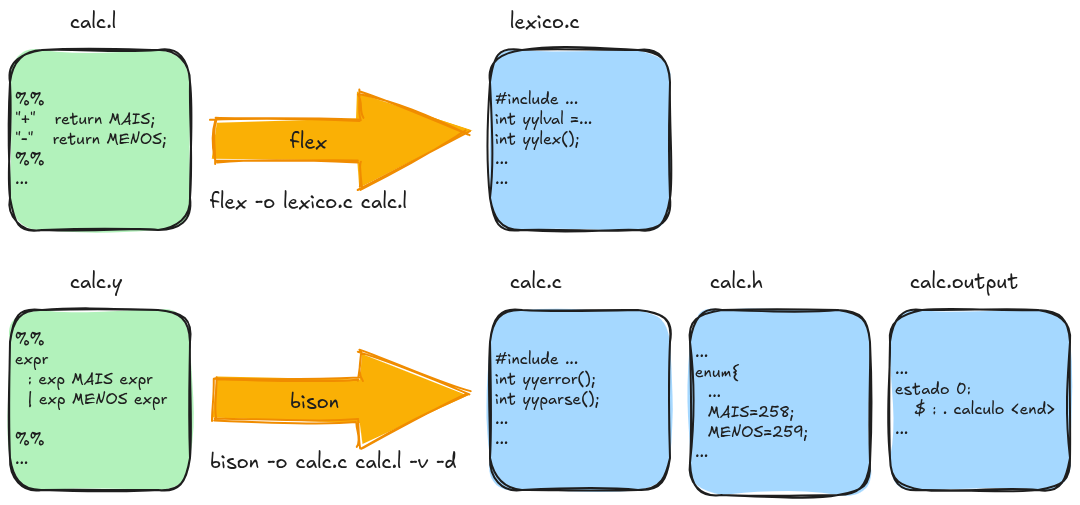
\includegraphics[width=0.9\linewidth,height=\textheight,keepaspectratio]{chapters/images/flex-bison.png}

}

\caption{\label{fig-flex-bison}Processo de construção da calculadora}

\end{figure}%

A figura apresenta, de forma esquemática, a \textbf{integração entre o
analisador léxico e o analisador sintático na utilização conjunta de
Flex e Bison}. O fluxo pode ser explicado a partir dos arquivos de
especificação, dos arquivos gerados pelas ferramentas e da comunicação
estabelecida entre os componentes.

O processo começa com o arquivo \textbf{\texttt{calc.l}}, que contém a
especificação do analisador léxico. Nele são definidas as expressões
regulares responsáveis por reconhecer os diferentes elementos da
linguagem. No exemplo, as regras reconhecem os operadores \texttt{+} e
\texttt{-} e retornam, respectivamente, os tokens \texttt{MAIS} e
\texttt{MENOS}. O arquivo também pode conter regras para números,
identificadores, espaços em branco e outros elementos léxicos.

A partir de \texttt{calc.l}, o \textbf{Flex} gera o arquivo
\textbf{\texttt{lexico.c}}. Esse arquivo contém a implementação do
analisador léxico, incluindo a função \texttt{yylex()}, responsável por
percorrer a entrada e identificar os tokens. A geração pode ser
realizada, por exemplo, pelo comando:

\begin{Shaded}
\begin{Highlighting}[]
\FunctionTok{flex} \AttributeTok{{-}o}\NormalTok{ lexico.c calc.l}
\end{Highlighting}
\end{Shaded}

Assim, o arquivo escrito pelo programador (\texttt{calc.l}) constitui a
especificação do analisador, enquanto \texttt{lexico.c} corresponde ao
código-fonte C produzido automaticamente pelo Flex.

De maneira semelhante, o arquivo \textbf{\texttt{calc.y}} contém a
especificação do analisador sintático. Nesse arquivo são declarados os
tokens utilizados pela gramática e definidas as produções que descrevem
a estrutura sintática das expressões. No exemplo representado na figura,
a gramática contém produções para expressões envolvendo os tokens
\texttt{MAIS} e \texttt{MENOS}. As regras podem ainda ser acompanhadas
de ações semânticas, responsáveis por realizar algum processamento
quando uma produção é reduzida.

O \textbf{Bison} recebe \texttt{calc.y} e gera o arquivo
\textbf{\texttt{calc.c}}, que implementa o analisador sintático.
Internamente, o Bison constrói as estruturas necessárias para realizar a
análise ascendente, incluindo os estados do autômato e a tabela de
análise sintática. A opção \texttt{-v} pode ser utilizada para solicitar
a geração de um arquivo contendo informações detalhadas sobre os estados
e as ações do analisador, enquanto a opção \texttt{-d} solicita a
geração de um arquivo de cabeçalho com as definições dos tokens.

O arquivo \textbf{\texttt{calc.h}} desempenha um papel importante na
integração entre o analisador léxico e o analisador sintático. Ele
contém as definições dos tokens gerados pelo Bison. Na figura, por
exemplo, aparecem códigos como \texttt{MAIS\ =\ 258} e
\texttt{MENOS\ =\ 259}. Dessa forma, tanto o código gerado pelo Flex
quanto o código gerado pelo Bison utilizam a mesma representação
numérica para os tokens.

A comunicação entre os dois analisadores ocorre principalmente por meio
da função \textbf{\texttt{yylex()}}. Quando o analisador sintático
necessita de um novo token, ele solicita esse token ao analisador
léxico. O \texttt{yylex()} examina a entrada, reconhece o próximo lexema
e retorna o código correspondente ao token. Por exemplo, ao encontrar o
caractere \texttt{+}, o analisador léxico pode retornar \texttt{MAIS};
ao encontrar \texttt{-}, pode retornar \texttt{MENOS}.

Além do código do token, o analisador léxico pode fornecer um
\textbf{valor semântico} associado ao token. Esse mecanismo é utilizado,
por exemplo, quando um número inteiro é reconhecido. Nesse caso, o texto
identificado pelo Flex pode ser convertido para um valor numérico e
armazenado em \texttt{yylval}, permitindo que o analisador sintático e
suas ações semânticas tenham acesso ao valor reconhecido.

A figura também mostra o arquivo \textbf{\texttt{calc.output}},
produzido quando o Bison é executado com a opção \texttt{-v}. Esse
arquivo é particularmente útil para compreender o funcionamento interno
do analisador. Ele apresenta informações sobre os \textbf{estados do
autômato LR}, os itens que compõem cada estado e as ações de
deslocamento e redução associadas aos símbolos da gramática. O trecho
apresentado na figura, por exemplo, mostra o estado inicial contendo um
item semelhante a:

\begin{Shaded}
\begin{Highlighting}[]
\NormalTok{estado 0:}

\NormalTok{    $ : . calculo \textless{}end\textgreater{}}
\end{Highlighting}
\end{Shaded}

O ponto indica a posição corrente durante a construção do item LR. Nesse
caso, o analisador encontra-se no estado inicial e ainda não reconheceu
nenhum símbolo da produção.

Finalmente, o arquivo \textbf{\texttt{calc.c}}, juntamente com o código
gerado pelo Flex e os demais arquivos necessários, pode ser compilado
para produzir o programa executável. O resultado é um analisador
sintático capaz de receber uma sequência de caracteres, solicitar tokens
ao analisador léxico e verificar se essa sequência pode ser reconhecida
pela gramática especificada em \texttt{calc.y}.

\subsection{Integração entre Lex/Flex e
Yacc/Bison}\label{integrauxe7uxe3o-entre-lexflex-e-yaccbison}

A construção de um analisador sintático com Yacc normalmente envolve sua
integração com um analisador léxico, tradicionalmente implementado com
\textbf{Lex} ou, atualmente, com ferramentas compatíveis como
\textbf{Flex}.

O analisador léxico é responsável por ler os caracteres da entrada e
agrupá-los em \textbf{tokens}. O analisador sintático, por sua vez,
recebe esses tokens e verifica se a sequência obtida está de acordo com
a gramática.

Por exemplo, podemos declarar um token para representar números
inteiros:

\begin{Shaded}
\begin{Highlighting}[]
\OperatorTok{\%}\NormalTok{token MAIS}
\OperatorTok{\%}\NormalTok{token NUMERO}
\end{Highlighting}
\end{Shaded}

A partir dessa declaração, o Yacc identifica \texttt{NUMERO} como um dos
terminais utilizados pela gramática. Durante a geração do analisador,
são produzidas as estruturas necessárias para que o analisador léxico e
o analisador sintático utilizem uma representação comum dos tokens.

O arquivo gerado contém, entre outras informações, os códigos numéricos
associados aos tokens. O analisador léxico pode então incluir o arquivo
de cabeçalho produzido pelo Yacc/Bison para ter acesso às definições
desses tokens.

A comunicação entre o analisador léxico e o sintático ocorre,
tradicionalmente, por meio da função \texttt{yylex()}. Quando o
analisador sintático necessita de um novo token, ele chama essa função.
O analisador léxico identifica o próximo elemento da entrada e retorna o
código correspondente ao token.

Além do código do token, o analisador léxico pode fornecer um
\textbf{valor associado} ao token por meio da variável \texttt{yylval}.
Esse mecanismo é particularmente importante para tokens que carregam
informações adicionais, como números, identificadores e literais.

Por exemplo, ao reconhecer um número inteiro, o analisador léxico pode
executar:

\begin{Shaded}
\begin{Highlighting}[]
\OperatorTok{[}\DecValTok{0}\OperatorTok{{-}}\DecValTok{9}\OperatorTok{]+} \OperatorTok{\{}
\NormalTok{    yylval }\OperatorTok{=}\NormalTok{ atoi}\OperatorTok{(}\NormalTok{yytext}\OperatorTok{);}
    \ControlFlowTok{return}\NormalTok{ NUMERO}\OperatorTok{;}
\OperatorTok{\}}
\end{Highlighting}
\end{Shaded}

Nesse caso, \texttt{yytext} contém o texto reconhecido pelo analisador
léxico. A função \texttt{atoi()} converte esse texto para um valor
inteiro, que é armazenado em \texttt{yylval}. Em seguida, a função
retorna o token \texttt{NUMERO} para o analisador sintático.

O tipo de \texttt{yylval} é determinado pela definição de
\texttt{YYSTYPE}. Em exemplos simples, pode ser utilizado o tipo
\texttt{int}. Em compiladores mais complexos, entretanto, diferentes
tokens podem transportar diferentes tipos de informação, como valores
numéricos, nomes de identificadores ou estruturas de dados.

\subsection{Pilhas utilizadas pelo analisador
sintático}\label{pilhas-utilizadas-pelo-analisador-sintuxe1tico}

Durante a análise, o Yacc mantém informações que representam o estado
corrente do processo de reconhecimento. Didaticamente, podemos
considerar duas estruturas principais: a \textbf{pilha de análise} e a
\textbf{pilha de valores}.

A pilha de análise representa a estrutura sintática que está sendo
construída. Nela são mantidas informações relacionadas aos símbolos e
aos estados do analisador. A pilha de valores, por sua vez, mantém os
valores semânticos associados aos símbolos.

As duas estruturas permanecem sincronizadas. Quando um token é deslocado
para a pilha durante uma operação \emph{shift}, seu valor correspondente
também é armazenado na estrutura de valores.

Durante uma redução, os símbolos correspondentes ao lado direito da
produção são removidos e substituídos pelo não terminal do lado
esquerdo. Simultaneamente, a ação semântica associada à produção pode
calcular o valor que será associado ao novo símbolo.

Considere a produção:

\begin{Shaded}
\begin{Highlighting}[]
\NormalTok{expr}\OperatorTok{:}
\NormalTok{      expr MAIS expr   }\OperatorTok{\{}\NormalTok{ $$ }\OperatorTok{=}\NormalTok{ $}\DecValTok{1} \OperatorTok{+}\NormalTok{ $}\DecValTok{3}\OperatorTok{;} \OperatorTok{\}}
\end{Highlighting}
\end{Shaded}

Os símbolos \texttt{\$1}, \texttt{\$2} e \texttt{\$3} representam os
valores associados aos símbolos que aparecem no lado direito da
produção. Nesse caso:

\begin{itemize}
\tightlist
\item
  \texttt{\$1} representa o valor da primeira ocorrência de
  \texttt{expr};
\item
  \texttt{\$2} representa o valor associado ao token \texttt{MAIS};
\item
  \texttt{\$3} representa o valor da segunda ocorrência de
  \texttt{expr};
\item
  \texttt{\$\$} representa o valor associado ao não terminal
  \texttt{expr} após a redução.
\end{itemize}

Assim, a ação:

\begin{Shaded}
\begin{Highlighting}[]
\OperatorTok{\{}\NormalTok{ $$ }\OperatorTok{=}\NormalTok{ $}\DecValTok{1} \OperatorTok{+}\NormalTok{ $}\DecValTok{3}\OperatorTok{;} \OperatorTok{\}}
\end{Highlighting}
\end{Shaded}

calcula o valor da expressão resultante e o associa ao símbolo
\texttt{expr} produzido pela redução.

Quando a produção é:

\begin{Shaded}
\begin{Highlighting}[]
\NormalTok{expr}\OperatorTok{:}
\NormalTok{      NUMERO   }\OperatorTok{\{}\NormalTok{ $$ }\OperatorTok{=}\NormalTok{ $}\DecValTok{1}\OperatorTok{;} \OperatorTok{\}}
\end{Highlighting}
\end{Shaded}

o valor do token \texttt{NUMERO} é simplesmente transferido para o não
terminal \texttt{expr}. Essa ação permite que o valor numérico
reconhecido pelo analisador léxico seja propagado pela árvore sintática
durante as reduções.

Esse mecanismo estabelece uma ligação direta entre a \textbf{análise
sintática} e a \textbf{análise semântica}. Enquanto as produções
determinam a estrutura sintática da linguagem, as ações semânticas
permitem associar informações e operações a essa estrutura.

\subsection{Exemplo de uma calculadora
simples}\label{exemplo-de-uma-calculadora-simples}

Os padrões léxicos utilizados nas expressões aritméticas é especificada
da seguinte forma para flex (arquivo \texttt{calc.l}):

\begin{Shaded}
\begin{Highlighting}[]
\OperatorTok{\%\{}
\PreprocessorTok{\#include }\ImportTok{"calc.h"}
\DataTypeTok{void}\NormalTok{ yyerror}\OperatorTok{(}\DataTypeTok{char} \OperatorTok{*);}
\OperatorTok{\%\}}

\OperatorTok{\%\%}
\OperatorTok{[}\DecValTok{0}\OperatorTok{{-}}\DecValTok{9}\OperatorTok{]+}     \OperatorTok{\{}  
\NormalTok{              yylval }\OperatorTok{=}\NormalTok{ atoi}\OperatorTok{(}\NormalTok{yytext}\OperatorTok{);}
              \ControlFlowTok{return}\NormalTok{ NUMERO}\OperatorTok{;}
           \OperatorTok{\}}
\StringTok{"+"}        \ControlFlowTok{return}\NormalTok{ MAIS}\OperatorTok{;}
\StringTok{"{-}"}        \ControlFlowTok{return}\NormalTok{ MENOS}\OperatorTok{;}
\StringTok{"*"}        \ControlFlowTok{return}\NormalTok{ VEZES}\OperatorTok{;}
\StringTok{"/"}        \ControlFlowTok{return}\NormalTok{ DIV}\OperatorTok{;}
\StringTok{"("}        \ControlFlowTok{return}\NormalTok{ ABRE}\OperatorTok{;}
\StringTok{")"}        \ControlFlowTok{return}\NormalTok{ FECHA}\OperatorTok{;}
\OperatorTok{[}\NormalTok{ \textbackslash{}t}\OperatorTok{]+}     \OperatorTok{;}
\NormalTok{\textbackslash{}n         }\ControlFlowTok{return}\NormalTok{ ENTER}\OperatorTok{;}
\OperatorTok{.}          \OperatorTok{\{}
             \DataTypeTok{char}\NormalTok{ msg}\OperatorTok{[}\DecValTok{100}\OperatorTok{];}
\NormalTok{             sprintf}\OperatorTok{(}\NormalTok{msg}\OperatorTok{,} \StringTok{"[}\SpecialCharTok{\%s}\StringTok{] desconhecido!"}\OperatorTok{,}\NormalTok{ yytext}\OperatorTok{);}
\NormalTok{             yyerror}\OperatorTok{(}\NormalTok{msg}\OperatorTok{);}
           \OperatorTok{\}}
\OperatorTok{\%\%}

\DataTypeTok{int}\NormalTok{ yywrap }\OperatorTok{()} \OperatorTok{\{}
    \ControlFlowTok{return} \DecValTok{1}\OperatorTok{;}
\OperatorTok{\}}
\end{Highlighting}
\end{Shaded}

Uma gramática elementar para uma calculadora que realiza operações de
adição, subtração, multiplicação, divisão e expressões entre parênteses
pode ser especificada como (arquivo \texttt{calc.y}):

\begin{Shaded}
\begin{Highlighting}[]
\OperatorTok{\%\{}
\PreprocessorTok{\#include }\ImportTok{\textless{}stdio.h\textgreater{}}
\PreprocessorTok{\#include }\ImportTok{\textless{}stdlib.h\textgreater{}}
\DataTypeTok{int}\NormalTok{ yylex}\OperatorTok{(}\DataTypeTok{void}\OperatorTok{);}
\DataTypeTok{void}\NormalTok{ yyerror}\OperatorTok{(}\DataTypeTok{char} \OperatorTok{*);}
\OperatorTok{\%\}}

\OperatorTok{\%}\NormalTok{token ENTER}
\OperatorTok{\%}\NormalTok{token MAIS}
\OperatorTok{\%}\NormalTok{token MENOS}
\OperatorTok{\%}\NormalTok{token VEZES}
\OperatorTok{\%}\NormalTok{token DIV}
\OperatorTok{\%}\NormalTok{token NUMERO}
\OperatorTok{\%}\NormalTok{token ABRE}
\OperatorTok{\%}\NormalTok{token FECHA}

\OperatorTok{\%}\NormalTok{start linha}

\OperatorTok{\%}\NormalTok{left MAIS MENOS }
\OperatorTok{\%}\NormalTok{left VEZES DIV}

\OperatorTok{\%\%}

\NormalTok{calculo}\OperatorTok{:}\NormalTok{ calculo expr ENTER }\OperatorTok{\{}\NormalTok{ printf }\OperatorTok{(}\StringTok{"resultado = }\SpecialCharTok{\%d\textbackslash{}n}\StringTok{"}\OperatorTok{,}\NormalTok{ $}\DecValTok{2}\OperatorTok{);} \OperatorTok{\}}
       \OperatorTok{|} 
       \OperatorTok{;}

\NormalTok{expr }\OperatorTok{:}\NormalTok{ expr MAIS expr }\OperatorTok{\{}\NormalTok{ $$ }\OperatorTok{=}\NormalTok{ $}\DecValTok{1} \OperatorTok{+}\NormalTok{ $}\DecValTok{3}\OperatorTok{;} \OperatorTok{\}}
     \OperatorTok{|}\NormalTok{ expr MENOS expr }\OperatorTok{\{}\NormalTok{ $$ }\OperatorTok{=}\NormalTok{ $}\DecValTok{1} \OperatorTok{{-}}\NormalTok{ $}\DecValTok{3}\OperatorTok{;} \OperatorTok{\}}
     \OperatorTok{|}\NormalTok{ expr VEZES expr }\OperatorTok{\{}\NormalTok{ $$ }\OperatorTok{=}\NormalTok{ $}\DecValTok{1} \OperatorTok{*}\NormalTok{ $}\DecValTok{3}\OperatorTok{;} \OperatorTok{\}}
     \OperatorTok{|}\NormalTok{ expr DIV expr   }\OperatorTok{\{}\NormalTok{ $$ }\OperatorTok{=}\NormalTok{ $}\DecValTok{1} \OperatorTok{/}\NormalTok{ $}\DecValTok{3}\OperatorTok{;} \OperatorTok{\}}
     \OperatorTok{|}\NormalTok{ ABRE expr FECHA }\OperatorTok{\{}\NormalTok{ $$ }\OperatorTok{=}\NormalTok{ $}\DecValTok{2}\OperatorTok{;} \OperatorTok{\}}
     \OperatorTok{|}\NormalTok{ NUMERO }\OperatorTok{\{}\NormalTok{ $$ }\OperatorTok{=}\NormalTok{ $}\DecValTok{1}\OperatorTok{;} \OperatorTok{\}}
     \OperatorTok{;}

\OperatorTok{\%\%}

\DataTypeTok{void}\NormalTok{ yyerror }\OperatorTok{(}\DataTypeTok{char} \OperatorTok{*}\NormalTok{msg}\OperatorTok{)} \OperatorTok{\{}
\NormalTok{    printf}\OperatorTok{(}\StringTok{"Erro: }\SpecialCharTok{\%s\textbackslash{}n}\StringTok{"}\OperatorTok{,}\NormalTok{ msg}\OperatorTok{);}
\OperatorTok{\}} 

\DataTypeTok{int}\NormalTok{ main}\OperatorTok{()} \OperatorTok{\{}
\NormalTok{    yyparse}\OperatorTok{();}
    \ControlFlowTok{return} \DecValTok{0}\OperatorTok{;}
\OperatorTok{\}}
\end{Highlighting}
\end{Shaded}

A produção \texttt{calculo} permite reconhecer uma sequência de
expressões, cada uma terminada por uma quebra de linha. Quando uma
expressão é reconhecida, seu valor é apresentado na saída.

A produção:

\begin{Shaded}
\begin{Highlighting}[]
\NormalTok{expr}\OperatorTok{:}\NormalTok{ expr MAIS expr}
\end{Highlighting}
\end{Shaded}

define uma expressão como a soma de duas outras expressões. Quando essa
produção é reduzida, a ação semântica calcula a soma dos valores
associados às duas subexpressões.

De maneira análoga:

\begin{Shaded}
\begin{Highlighting}[]
\NormalTok{expr}\OperatorTok{:}\NormalTok{ expr MENOS expr}
\end{Highlighting}
\end{Shaded}

calcula a diferença entre os valores das duas expressões.

O uso de ações semânticas dessa forma permite que o analisador não
apenas reconheça se uma sequência pertence à linguagem definida pela
gramática, mas também \textbf{execute operações associadas à estrutura
sintática reconhecida}.

Esse processo está ilustrado na árvore de derivação apresentada na
Figura~\ref{fig-arvore-expressao}. As ações semânticas associadas às
produções podem ser entendidas como operações executadas durante o
processo de análise sintática, à medida que o analisador percorre a
árvore de derivação. Quando uma ação semântica é alcançada, ela é
executada e os valores associados aos símbolos da árvore são calculados
ou atualizados. Dessa forma, as informações semânticas são propagadas
pela árvore, permitindo que o valor de uma construção sintática seja
determinado a partir dos valores de seus componentes.

\begin{figure}

\centering{

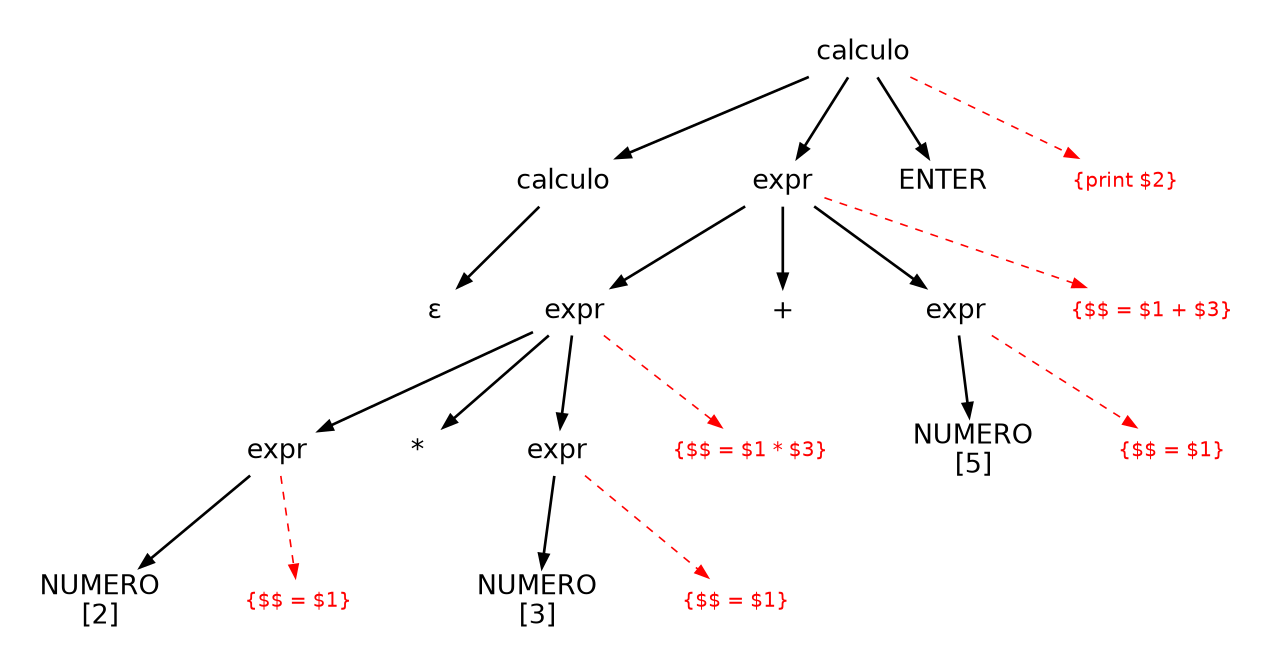
\includegraphics[width=0.9\linewidth,height=\textheight,keepaspectratio]{chapters/images/arvore-expressao.png}

}

\caption{\label{fig-arvore-expressao}Árvore de Derivação para expressão
\texttt{2\ *\ 3\ +\ 5}}

\end{figure}%

Esse princípio é fundamental para a construção de compiladores. Durante
a análise sintática, as reduções podem ser utilizadas para construir
árvores sintáticas, verificar informações semânticas, gerar
representações intermediárias ou executar ações específicas associadas
às construções da linguagem.

Para geração da calculadora devemos executar a seguinte sequência de
comandos:

\begin{Shaded}
\begin{Highlighting}[]
\NormalTok{flex }\OperatorTok{{-}}\NormalTok{o lexico}\OperatorTok{.}\NormalTok{c calc}\OperatorTok{.}\NormalTok{l}
\NormalTok{bison }\OperatorTok{{-}}\NormalTok{o calc}\OperatorTok{.}\NormalTok{c calc}\OperatorTok{.}\NormalTok{y }\OperatorTok{{-}}\NormalTok{v }\OperatorTok{{-}}\NormalTok{d}\OperatorTok{;}
\NormalTok{gcc lexico}\OperatorTok{.}\NormalTok{c calc}\OperatorTok{.}\NormalTok{c }\OperatorTok{{-}}\NormalTok{o calc}\OperatorTok{;}
\end{Highlighting}
\end{Shaded}

\subsection{Tratamento de erros
sintáticos}\label{tratamento-de-erros-sintuxe1ticos}

Quando o analisador sintático encontra uma sequência de tokens que não
pode ser derivada pela gramática, ocorre um \textbf{erro sintático}. O
Yacc/Bison disponibiliza mecanismos para tratar esses erros,
tradicionalmente por meio da função \texttt{yyerror()}.

Uma implementação simples pode ser:

\begin{Shaded}
\begin{Highlighting}[]
\DataTypeTok{void}\NormalTok{ yyerror}\OperatorTok{(}\DataTypeTok{char} \OperatorTok{*}\NormalTok{s}\OperatorTok{)}
\OperatorTok{\{}
\NormalTok{    printf}\OperatorTok{(}\StringTok{"}\SpecialCharTok{\%s\textbackslash{}n}\StringTok{"}\OperatorTok{,}\NormalTok{ s}\OperatorTok{);}
\OperatorTok{\}}
\end{Highlighting}
\end{Shaded}

Essa função recebe uma mensagem associada ao erro detectado pelo
analisador sintático e pode ser modificada para produzir mensagens mais
informativas, incluindo, por exemplo, a linha e a coluna em que o erro
ocorreu, o token encontrado e os tokens esperados.

O tratamento de erros é uma característica importante de analisadores
sintáticos utilizados em compiladores reais. Um compilador não deve
apenas detectar que uma entrada é inválida, mas também fornecer
informações que auxiliem o programador a localizar e corrigir o
problema.

\subsection{Uso da calculadora de
expressões}\label{uso-da-calculadora-de-expressuxf5es}

Com o executável gerado \texttt{calc} podemos realizar alguns cálculos:

\begin{Shaded}
\begin{Highlighting}[]
\NormalTok{$ }\OperatorTok{./}\NormalTok{calc}
\DecValTok{12} \OperatorTok{+} \DecValTok{4}
\NormalTok{resultado }\OperatorTok{=} \DecValTok{16}
\DecValTok{2} \OperatorTok{*} \OperatorTok{(}\DecValTok{3} \OperatorTok{+} \DecValTok{4}\OperatorTok{)}
\NormalTok{resultado }\OperatorTok{=} \DecValTok{14}
\DecValTok{2} \OperatorTok{+} \DecValTok{3} \OperatorTok{+} \DecValTok{4}
\NormalTok{resultado }\OperatorTok{=} \DecValTok{9}
\OperatorTok{\^{}}\NormalTok{C}
\NormalTok{$ }
\end{Highlighting}
\end{Shaded}

\section{Geração de código para a Máquina Virtual
Simples}\label{gerauxe7uxe3o-de-cuxf3digo-para-a-muxe1quina-virtual-simples}

A tradução dirigida por sintaxe permite integrar a geração de código ao
analisador sintático. Quando uma produção é reconhecida, sua ação
semântica pode emitir as instruções necessárias para representar a
construção correspondente.

Neste capítulo, utilizaremos a Máquina Virtual Simples (MVS) como
destino para exemplificar esse processo. A MVS possui instruções para
carregar constantes, acessar variáveis, realizar operações aritméticas e
armazenar resultados. Sua arquitetura baseada em pilha permite
compreender como as expressões são traduzidas sem exigir, inicialmente,
o estudo de registradores de uma arquitetura real.

Considere o seguinte fragmento de gramática, escrito no estilo do Bison:

\begin{Shaded}
\begin{Highlighting}[]
\NormalTok{cmd }\OperatorTok{:}
\NormalTok{      expr}
        \OperatorTok{\{} \OperatorTok{\}}
    \OperatorTok{|}\NormalTok{ VAR ATRIBUI expr}
        \OperatorTok{\{}\NormalTok{ printf}\OperatorTok{(}\StringTok{"}\SpecialCharTok{\textbackslash{}t}\StringTok{ARZG}\SpecialCharTok{\textbackslash{}t\%d\textbackslash{}n}\StringTok{"}\OperatorTok{,}\NormalTok{ $}\DecValTok{1}\OperatorTok{);} \OperatorTok{\}}
    \OperatorTok{;}

\NormalTok{expr }\OperatorTok{:}
\NormalTok{      NUM}
        \OperatorTok{\{}\NormalTok{ printf}\OperatorTok{(}\StringTok{"}\SpecialCharTok{\textbackslash{}t}\StringTok{CRCT}\SpecialCharTok{\textbackslash{}t\%d\textbackslash{}n}\StringTok{"}\OperatorTok{,}\NormalTok{ $}\DecValTok{1}\OperatorTok{);} \OperatorTok{\}}
    \OperatorTok{|}\NormalTok{ VAR}
        \OperatorTok{\{}\NormalTok{ printf}\OperatorTok{(}\StringTok{"}\SpecialCharTok{\textbackslash{}t}\StringTok{CRVG}\SpecialCharTok{\textbackslash{}t\%d\textbackslash{}n}\StringTok{"}\OperatorTok{,}\NormalTok{ $}\DecValTok{1}\OperatorTok{);} \OperatorTok{\}}
    \OperatorTok{|}\NormalTok{ expr MAIS expr}
        \OperatorTok{\{}\NormalTok{ printf}\OperatorTok{(}\StringTok{"}\SpecialCharTok{\textbackslash{}t}\StringTok{SOMA}\SpecialCharTok{\textbackslash{}n}\StringTok{"}\OperatorTok{);} \OperatorTok{\}}
    \OperatorTok{|}\NormalTok{ expr MENOS expr}
        \OperatorTok{\{}\NormalTok{ printf}\OperatorTok{(}\StringTok{"}\SpecialCharTok{\textbackslash{}t}\StringTok{SUBT}\SpecialCharTok{\textbackslash{}n}\StringTok{"}\OperatorTok{);} \OperatorTok{\}}
    \OperatorTok{|}\NormalTok{ expr BARRA expr}
        \OperatorTok{\{}\NormalTok{ printf}\OperatorTok{(}\StringTok{"}\SpecialCharTok{\textbackslash{}t}\StringTok{DIVI}\SpecialCharTok{\textbackslash{}n}\StringTok{"}\OperatorTok{);} \OperatorTok{\}}
    \OperatorTok{|}\NormalTok{ expr VEZES expr}
        \OperatorTok{\{}\NormalTok{ printf}\OperatorTok{(}\StringTok{"}\SpecialCharTok{\textbackslash{}t}\StringTok{MULT}\SpecialCharTok{\textbackslash{}n}\StringTok{"}\OperatorTok{);} \OperatorTok{\}}
    \OperatorTok{|}\NormalTok{ ABRE expr FECHA}
        \OperatorTok{\{} \OperatorTok{\}}
    \OperatorTok{;}
\end{Highlighting}
\end{Shaded}

Nesse fragmento, \texttt{cmd} representa um comando, enquanto
\texttt{expr} representa uma expressão aritmética. Os nomes
\texttt{NUM}, \texttt{VAR}, \texttt{ATRIBUI}, \texttt{MAIS},
\texttt{MENOS}, \texttt{BARRA}, \texttt{VEZES}, \texttt{ABRE} e
\texttt{FECHA} representam tokens definidos pelo analisador léxico.

As ações semânticas produzem instruções da MVS conforme as construções
reconhecidas:

\begin{itemize}
\tightlist
\item
  \texttt{CRCT} carrega uma constante na pilha.
\item
  \texttt{CRVG} carrega na pilha o valor de uma variável.
\item
  \texttt{SOMA} remove os dois operandos do topo da pilha, soma seus
  valores e empilha o resultado.
\item
  \texttt{SUBT}, \texttt{MULT} e \texttt{DIVI} realizam as operações
  aritméticas correspondentes.
\item
  \texttt{ARZG} armazena o valor do topo da pilha no endereço da
  variável indicada.
\end{itemize}

As instruções emitidas para uma expressão devem respeitar a ordem de
execução da máquina. Primeiro são carregados os operandos; depois, a
instrução correspondente à operação é executada. Dessa forma, a
avaliação de uma expressão deixa de depender de uma ação direta sobre os
valores durante a compilação e passa a ser representada por instruções
que serão executadas posteriormente.

\subsection{Exemplo de geração de
código}\label{exemplo-de-gerauxe7uxe3o-de-cuxf3digo}

Considere o comando:

\begin{Shaded}
\begin{Highlighting}[]
\NormalTok{resultado \textless{}{-} }\DecValTok{10}\NormalTok{ + }\DecValTok{20}
\end{Highlighting}
\end{Shaded}

Suponha que o analisador léxico associe o endereço \texttt{3} à variável
\texttt{resultado}. Durante a análise sintática, a expressão
\texttt{10\ +\ 20} é reconhecida, e suas ações semânticas emitem as
instruções correspondentes. Ao final, a ação da atribuição armazena o
resultado no endereço da variável.

O código gerado será semelhante a:

\begin{Shaded}
\begin{Highlighting}[]
\KeywordTok{CRCT}    \DecValTok{10}
\KeywordTok{CRCT}    \DecValTok{20}
\KeywordTok{SOMA}
\KeywordTok{ARZG}    \DecValTok{3}
\end{Highlighting}
\end{Shaded}

A execução ocorre na seguinte ordem:

CRCT 10

Carregamento da primeira constante

O valor \texttt{10} é colocado no topo da pilha.

CRCT 20

Carregamento da segunda constante

O valor \texttt{20} é empilhado sobre o valor anterior.

SOMA

Operação aritmética

Os valores \texttt{10} e \texttt{20} são removidos da pilha, somados, e
o resultado \texttt{30} é colocado no topo.

ARZG 3

Armazenamento do resultado

O valor \texttt{30} é armazenado no endereço associado à variável
\texttt{resultado}.

O exemplo demonstra a relação entre a estrutura sintática do comando, as
ações semânticas executadas pelo analisador e o código produzido para a
MVS. A atribuição é reconhecida como um comando completo, mas as
instruções de cálculo da expressão são emitidas antes da instrução de
armazenamento.

Na implementação real, o endereço associado ao token \texttt{VAR} deve
ser obtido de uma tabela de símbolos ou de outra estrutura equivalente.
O exemplo pressupõe que \texttt{\$1} contenha esse endereço e que
\texttt{\$1} em \texttt{NUM} contenha o valor numérico do token.

Também é necessário configurar a gramática para respeitar a precedência
e a associatividade dos operadores. Sem essas declarações ou uma
gramática estruturada em níveis de precedência, expressões como
\texttt{2\ +\ 3\ *\ 4} podem gerar conflitos ou ser agrupadas de maneira
diferente da esperada. Além disso, o tratamento de divisões por zero e
outras condições de execução depende das regras adotadas pela MVS.

\subsection{Geração de código durante a análise
sintática}\label{gerauxe7uxe3o-de-cuxf3digo-durante-a-anuxe1lise-sintuxe1tica}

No exemplo anterior, o código é produzido diretamente pelas ações
semânticas do analisador sintático. Essa abordagem é simples e adequada
a compiladores didáticos, nos quais se deseja acompanhar a relação entre
uma produção gramatical e a instrução correspondente.

Entretanto, a geração direta apresenta limitações quando o compilador
precisa realizar otimizações, reorganizar instruções ou produzir código
para diferentes arquiteturas. Como as instruções são emitidas à medida
que a análise ocorre, pode ser necessário armazená-las, revisá-las ou
reconstruir partes do código para realizar transformações mais
complexas.

Uma alternativa consiste em construir uma representação intermediária
entre a análise semântica e a geração de código. Nesse modelo, as ações
semânticas produzem uma representação independente da máquina de
destino. Em uma etapa posterior, um gerador traduz essa representação
para as instruções da MVS.

Por exemplo, para o comando:

\begin{Shaded}
\begin{Highlighting}[]
\NormalTok{resultado \textless{}{-} }\DecValTok{10}\NormalTok{ + }\DecValTok{20}
\end{Highlighting}
\end{Shaded}

a representação intermediária poderia ser:

\begin{Shaded}
\begin{Highlighting}[]
\NormalTok{t1 }\OperatorTok{=} \DecValTok{10} \OperatorTok{+} \DecValTok{20}
\NormalTok{resultado }\OperatorTok{=}\NormalTok{ t1}
\end{Highlighting}
\end{Shaded}

O gerador de código transforma essas operações em instruções da MVS,
considerando a forma de acesso às variáveis e o funcionamento da pilha.
Essa separação permite alterar o gerador sem modificar a análise
sintática e possibilita aplicar otimizações sobre a representação
intermediária.

Portanto, existem duas estratégias complementares: emitir código
diretamente durante a análise sintática ou construir uma representação
intermediária para gerar o código em uma etapa posterior. A escolha
depende da complexidade do compilador e dos objetivos de sua
implementação.

Para um compilador simples, a geração direta facilita o entendimento do
processo. Para compiladores maiores, uma representação intermediária
tende a favorecer a organização, a manutenção e a implementação de
otimizações.

Em ambos os casos, a tradução dirigida por sintaxe estabelece uma
ligação explícita entre as regras da gramática e as operações
necessárias para traduzir o programa. Essa ligação permite compreender
como o compilador passa da identificação das construções sintáticas à
produção de instruções que preservam o significado do programa de
origem.

\subsection{Projeto do Compilador - Parte
3}\label{projeto-do-compilador---parte-3}

O projeto implementa um compilador para uma linguagem simples,
denominada nos arquivos como linguagem \texttt{simples}. O programa de
entrada contém declarações de variáveis e comandos de atribuição,
leitura, escrita, seleção e repetição. O compilador verifica a estrutura
sintática do programa, realiza verificações semânticas e produz um
arquivo contendo as instruções da MVS.

A implementação está distribuída em dois arquivos principais:

\begin{itemize}
\tightlist
\item
  \texttt{sintatico.y}: contém a gramática da linguagem, as ações
  semânticas associadas às produções e a rotina principal que controla a
  leitura do programa e a geração do arquivo de saída.
\item
  \texttt{utils.c}: contém as estruturas e funções auxiliares utilizadas
  na análise semântica, incluindo a tabela de símbolos, a pilha de tipos
  e as operações de verificação de compatibilidade.
\end{itemize}

O arquivo \texttt{sintatico.y} utiliza o Bison para gerar o analisador
sintático em C. Os tokens são fornecidos pelo analisador léxico,
responsável por reconhecer palavras reservadas, identificadores, números
e operadores. A comunicação entre as etapas ocorre por meio dos tokens e
das informações associadas a eles, como o conteúdo textual armazenado em
\texttt{atomo}.

Nesse projeto, não é construída uma representação intermediária completa
para depois gerar o código. As ações semânticas escrevem diretamente as
instruções da MVS no arquivo de saída. Essa escolha simplifica a
implementação e permite observar como cada construção da linguagem de
origem se transforma em instruções da máquina virtual.

\subsubsection{\texorpdfstring{O arquivo \texttt{utils.c}: estruturas de
apoio à análise
semântica}{O arquivo utils.c: estruturas de apoio à análise semântica}}\label{o-arquivo-utils.c-estruturas-de-apoio-uxe0-anuxe1lise-semuxe2ntica}

O arquivo \texttt{utils.c} reúne os mecanismos necessários para
armazenar informações sobre os identificadores, acompanhar os tipos das
expressões e detectar algumas inconsistências semânticas.

\subsubsection{Tabela de símbolos}\label{tabela-de-suxedmbolos-1}

A tabela de símbolos é implementada por meio de um vetor de estruturas:

\begin{Shaded}
\begin{Highlighting}[]
\CommentTok{/*{-}{-}{-}{-}{-}{-}{-}{-}{-}{-}{-}{-}{-}{-}{-}{-}{-}{-}{-}{-}{-}{-}{-}{-}{-}{-}{-}{-}{-}{-}{-}{-}{-}{-}{-}}
\CommentTok{ * Estrutura da Tabela de Símbolos}
\CommentTok{ *{-}{-}{-}{-}{-}{-}{-}{-}{-}{-}{-}{-}{-}{-}{-}{-}{-}{-}{-}{-}{-}{-}{-}{-}{-}{-}{-}{-}{-}{-}{-}{-}{-}{-}{-}*/}

\PreprocessorTok{\#define TAMTAB }\DecValTok{100}
\KeywordTok{typedef} \KeywordTok{struct}
\OperatorTok{\{}
    \DataTypeTok{char}\NormalTok{ nome}\OperatorTok{[}\DecValTok{30}\OperatorTok{];}
    \DataTypeTok{int}\NormalTok{ tipo}\OperatorTok{;}
    \DataTypeTok{int}\NormalTok{ end}\OperatorTok{;}
\OperatorTok{\}}\NormalTok{ tiptab}\OperatorTok{;}

\NormalTok{tiptab elemtab}\OperatorTok{,}\NormalTok{ tabsimb}\OperatorTok{[}\NormalTok{TAMTAB}\OperatorTok{];}
\DataTypeTok{int}\NormalTok{ topotab }\OperatorTok{=} \OperatorTok{{-}}\DecValTok{1}\OperatorTok{;}
\end{Highlighting}
\end{Shaded}

Cada elemento da tabela contém três informações:

\begin{itemize}
\tightlist
\item
  \texttt{nome}: nome do identificador;
\item
  \texttt{end}: endereço associado à variável na memória da MVS;
\item
  \texttt{tipo}: tipo da variável, que pode ser inteiro (\texttt{INT})
  ou lógico (\texttt{LOG}).
\end{itemize}

A constante \texttt{TAMTAB} estabelece a capacidade máxima da tabela, de
100 identificadores. A variável \texttt{topotab} indica a quantidade de
posições ocupadas e, consequentemente, a próxima posição disponível para
inserção.

\subsubsection{Inserção de
identificadores}\label{inseruxe7uxe3o-de-identificadores}

A função \texttt{inseresimbolo} recebe uma estrutura contendo as
informações de uma variável e a registra na tabela de símbolos. Antes da
inserção, verifica se a tabela está cheia e se o identificador já foi
declarado.

A detecção de identificadores duplicados evita que duas declarações
utilizem o mesmo nome, conforme as regras adotadas por essa
implementação. Caso o nome já esteja registrado, a função chama
\texttt{yyerror} para informar o problema.

Durante a análise das declarações, o compilador preenche os campos da
estrutura \texttt{elemTab} e chama essa função para registrar cada
variável. O endereço é atribuído sequencialmente por meio da variável
\texttt{contaVar}, enquanto o tipo é obtido da declaração
correspondente.

\subsubsection{Busca de identificadores}\label{busca-de-identificadores}

A função \texttt{buscasimbolo} procura um identificador pelo nome e
retorna sua posição na tabela. Ela é utilizada quando o programa faz
referência a uma variável, seja em uma expressão, em uma atribuição ou
em um comando de leitura.

Se o identificador não estiver cadastrado, a função comunica o erro por
meio de \texttt{yyerror}. Caso seja encontrado, o compilador pode
consultar seus campos \texttt{end} e \texttt{tip} para gerar o código
apropriado e verificar a compatibilidade de tipos.

A tabela de símbolos desempenha, portanto, duas funções importantes:
permite verificar se as variáveis foram declaradas e fornece os
endereços e tipos necessários às etapas seguintes da compilação.

\subsubsection{Pilha Semântica}\label{pilha-semuxe2ntica}

A verificação dos tipos das expressões, a resolução de rótulos nas
estruturas de seleção e repetição e outras situações da compilação são
resolvidas com o auxílio de uma pilha da pilha semântica

\begin{Shaded}
\begin{Highlighting}[]
\KeywordTok{enum}
\OperatorTok{\{}
\NormalTok{    INT }\OperatorTok{=} \DecValTok{10}\OperatorTok{,}
\NormalTok{    LOG }\OperatorTok{=} \DecValTok{20}
\OperatorTok{\};}

\CommentTok{/*{-}{-}{-}{-}{-}{-}{-}{-}{-}{-}{-}{-}{-}{-}{-}{-}{-}{-}{-}{-}{-}{-}{-}{-}{-}{-}{-}{-}{-}{-}{-}{-}{-}{-}{-}}
\CommentTok{ * Estrutura da Pilha Semantica}
\CommentTok{ *{-}{-}{-}{-}{-}{-}{-}{-}{-}{-}{-}{-}{-}{-}{-}{-}{-}{-}{-}{-}{-}{-}{-}{-}{-}{-}{-}{-}{-}{-}{-}{-}{-}{-}{-}*/}
\PreprocessorTok{\#define TAMPILHA }\DecValTok{100}
\KeywordTok{struct}
\OperatorTok{\{}
    \DataTypeTok{int}\NormalTok{ valor}\OperatorTok{;}
    \DataTypeTok{char}\NormalTok{ tipo}\OperatorTok{;}
\OperatorTok{\}}\NormalTok{ Pilha}\OperatorTok{[}\NormalTok{TAMPILHA}\OperatorTok{];}

\DataTypeTok{int}\NormalTok{ topo }\OperatorTok{=} \OperatorTok{{-}}\DecValTok{1}\OperatorTok{;}
\end{Highlighting}
\end{Shaded}

Os tipos são representados por constantes inteiras definidas no
\texttt{enum}. O tipo \texttt{INT} identifica valores inteiros, enquanto
\texttt{LOG} identifica valores lógicos. Esses tipos serão utilizados
durante a análise semântica para verificar se as operações e atribuições
são compatíveis com as regras da linguagem.

As funções \texttt{empilha} e \texttt{desempilha} inserem e removem
valores dessa estrutura, verificando seus limites. No compilador, os
valores armazenados representam os tipos das expressões reconhecidas, os
rótulos, posição de identificadores na tabela de símbolos e contagem de
variáveis na declaração.

A utilização de uma pilha é adequada à análise sintática ascendente
realizada pelo Bison para verificação de tipos nas expressões, por
exemplo. Quando uma expressão simples é reconhecida, seu tipo é colocado
na pilha. Quando uma produção combina duas expressões, seus tipos são
removidos, verificados e substituídos pelo tipo resultante.

A função \texttt{testatipo} implementa esse procedimento:

\begin{Shaded}
\begin{Highlighting}[]
\DataTypeTok{void}\NormalTok{ testatipo}\OperatorTok{(}\DataTypeTok{int}\NormalTok{ tipo1}\OperatorTok{,} \DataTypeTok{int}\NormalTok{ tipo2}\OperatorTok{,} \DataTypeTok{int}\NormalTok{ ret}\OperatorTok{)}
\OperatorTok{\{}
    \DataTypeTok{int}\NormalTok{ t2 }\OperatorTok{=}\NormalTok{ desempilha}\OperatorTok{(}\CharTok{\textquotesingle{}t\textquotesingle{}}\OperatorTok{);}
    \DataTypeTok{int}\NormalTok{ t1 }\OperatorTok{=}\NormalTok{ desempilha}\OperatorTok{(}\CharTok{\textquotesingle{}t\textquotesingle{}}\OperatorTok{);}

    \ControlFlowTok{if} \OperatorTok{(}\NormalTok{t1 }\OperatorTok{!=}\NormalTok{ tipo1 }\OperatorTok{||}\NormalTok{ t2 }\OperatorTok{!=}\NormalTok{ tipo2}\OperatorTok{)}
\NormalTok{        yyerror}\OperatorTok{(}\StringTok{"Incompatibilidade de tipo!"}\OperatorTok{);}

\NormalTok{    empilha}\OperatorTok{(}\NormalTok{ret}\OperatorTok{,} \CharTok{\textquotesingle{}t\textquotesingle{}}\OperatorTok{);}
\OperatorTok{\}}
\end{Highlighting}
\end{Shaded}

Os parâmetros \texttt{tipo1} e \texttt{tipo2} indicam os tipos esperados
para os operandos, e \texttt{ret} representa o tipo do resultado da
operação. Se os tipos encontrados não forem os esperados, o compilador
comunica uma incompatibilidade. Caso contrário, o tipo resultante é
colocado na pilha para ser utilizado pelas produções superiores.

Por exemplo, a soma exige dois operandos inteiros e produz um resultado
inteiro. Já uma comparação entre inteiros produz um valor lógico. Essa
diferença permite que o compilador verifique não apenas os operandos,
mas também o tipo produzido por cada operação.

\subsection{\texorpdfstring{O arquivo \texttt{sintatico.y}: análise
sintática, semântica e geração de
código}{O arquivo sintatico.y: análise sintática, semântica e geração de código}}\label{o-arquivo-sintatico.y-anuxe1lise-sintuxe1tica-semuxe2ntica-e-gerauxe7uxe3o-de-cuxf3digo}

O arquivo \texttt{sintatico.y} contém a especificação da gramática e as
ações semânticas que serão executadas durante o reconhecimento do
programa. Além de identificar as construções válidas da linguagem, essas
ações consultam a tabela de símbolos, verificam os tipos das expressões
e emitem instruções da MVS.

\subsubsection{Declarações e variáveis
globais}\label{declarauxe7uxf5es-e-variuxe1veis-globais}

No início do arquivo, são incluídas bibliotecas da linguagem C e o
arquivo \texttt{utils.c}. Também são declaradas funções e variáveis
externas utilizadas pelo analisador léxico e pelo sistema de entrada e
saída.

Entre as variáveis globais, destacam-se:

\begin{Shaded}
\begin{Highlighting}[]
\KeywordTok{extern} \DataTypeTok{int}\NormalTok{ nlinha}\OperatorTok{;}   \CommentTok{// numero da linha}
\DataTypeTok{int}\NormalTok{ contavar }\OperatorTok{=} \DecValTok{0}\OperatorTok{;}    \CommentTok{// contador de variveis}
\DataTypeTok{int}\NormalTok{ rotulo }\OperatorTok{=} \DecValTok{0}\OperatorTok{;}      \CommentTok{// contador de rotulos}
\DataTypeTok{int}\NormalTok{ tipo}\OperatorTok{;}            \CommentTok{// tipo da variavel}
\end{Highlighting}
\end{Shaded}

A variável \texttt{nlinha} é atualizada toda vez que o analisador léxico
passa pelo caracter \texttt{\textbackslash{}\textbackslash{}n}. A
variável \texttt{contavar} controla a quantidade de variáveis declaradas
e permite atribuir endereços sequenciais às posições de memória
utilizadas pelo programa. A variável \texttt{tipo} armazena
temporariamente o tipo da declaração em processamento. Já
\texttt{rotulo} controla a numeração dos rótulos utilizados nos comandos
de seleção e repetição.

Os rótulos são necessários porque as estruturas de controle geram
desvios no fluxo de execução. Uma instrução condicional pode transferir
o controle para uma posição posterior do código, enquanto um laço
precisa retornar a uma posição anterior para avaliar novamente sua
condição.

\subsubsection{Tokens e precedência dos
operadores}\label{tokens-e-preceduxeancia-dos-operadores}

As diretivas \texttt{\%token} declaram os símbolos terminais
reconhecidos pelo analisador léxico. Entre eles estão os tokens que
representam as palavras reservadas da linguagem, como
\texttt{T\_PROGRAMA}, \texttt{T\_INICIO}, \texttt{T\_FIM},
\texttt{T\_LEIA}, \texttt{T\_ESCREVA}, \texttt{T\_ENQTO} e
\texttt{T\_SE}.

Também são declarados tokens para identificadores, números, tipos,
operadores aritméticos, operadores relacionais e operadores lógicos.

As declarações de precedência estabelecem a prioridade relativa dos
operadores:

\begin{Shaded}
\begin{Highlighting}[]
\OperatorTok{\%}\NormalTok{left T\_E T\_OU}
\OperatorTok{\%}\NormalTok{left T\_IGUAL}
\OperatorTok{\%}\NormalTok{left T\_MAIOR T\_MENOR}
\OperatorTok{\%}\NormalTok{left T\_MAIS T\_MENOS}
\OperatorTok{\%}\NormalTok{left T\_VEZES T\_DIV}
\end{Highlighting}
\end{Shaded}

A diretiva \texttt{\%left} indica associatividade à esquerda. No Bison,
as declarações posteriores possuem maior precedência que as anteriores.
Assim, a ordem apresentada estabelece a multiplicação e a divisão como
operadores de maior precedência entre os declarados, seguidas pela
adição e subtração, pelos operadores relacionais e pela igualdade,
ficando os operadores lógicos \texttt{E} e \texttt{OU} no nível mais
baixo.

Essa organização permite interpretar expressões como:

\begin{Shaded}
\begin{Highlighting}[]
\DecValTok{3}\NormalTok{ + }\DecValTok{4}\NormalTok{ * }\DecValTok{5}
\end{Highlighting}
\end{Shaded}

de modo que a multiplicação seja realizada antes da adição. A
precedência definida pelo analisador é essencial para que a estrutura
sintática e o código gerado correspondam à interpretação esperada da
expressão.

\subsubsection{Estrutura geral do
programa}\label{estrutura-geral-do-programa}

A produção inicial é declarada pela diretiva:

\begin{Shaded}
\begin{Highlighting}[]
\OperatorTok{\%}\NormalTok{start programa}
\end{Highlighting}
\end{Shaded}

Isso estabelece \texttt{programa} como o símbolo inicial da gramática. A
produção correspondente define a organização geral de um programa-fonte:

\begin{Shaded}
\begin{Highlighting}[]
\NormalTok{programa}
    \OperatorTok{:}\NormalTok{ cabecalho }
         \OperatorTok{\{}\NormalTok{ fprintf}\OperatorTok{(}\NormalTok{yyout}\OperatorTok{,} \StringTok{"}\SpecialCharTok{\textbackslash{}t}\StringTok{INPP}\SpecialCharTok{\textbackslash{}n}\StringTok{"}\OperatorTok{);} \OperatorTok{\}}
\NormalTok{      variaveis }
         \OperatorTok{\{} 
\NormalTok{            DEBUG}\OperatorTok{(}\NormalTok{mostratabela}\OperatorTok{();)}
\NormalTok{            empilha}\OperatorTok{(}\NormalTok{contavar}\OperatorTok{,} \CharTok{\textquotesingle{}c\textquotesingle{}}\OperatorTok{);}
            \ControlFlowTok{if} \OperatorTok{(}\NormalTok{contavar }\OperatorTok{\textgreater{}} \DecValTok{0}\OperatorTok{)} \OperatorTok{\{}
\NormalTok{               fprintf}\OperatorTok{(}\NormalTok{yyout}\OperatorTok{,} \StringTok{"}\SpecialCharTok{\textbackslash{}t}\StringTok{AMEM}\SpecialCharTok{\textbackslash{}t\%d\textbackslash{}n}\StringTok{"}\OperatorTok{,}\NormalTok{ contavar}\OperatorTok{);}
            \OperatorTok{\}} 
         \OperatorTok{\}}
\NormalTok{      T\_INICIO lista\_comandos T\_FIM}
         \OperatorTok{\{}
            \DataTypeTok{int}\NormalTok{ conta }\OperatorTok{=}\NormalTok{ desempilha}\OperatorTok{(}\CharTok{\textquotesingle{}c\textquotesingle{}}\OperatorTok{);}
            \ControlFlowTok{if} \OperatorTok{(}\NormalTok{conta }\OperatorTok{\textgreater{}} \DecValTok{0}\OperatorTok{)} 
\NormalTok{               fprintf}\OperatorTok{(}\NormalTok{yyout}\OperatorTok{,} \StringTok{"}\SpecialCharTok{\textbackslash{}t}\StringTok{DMEM}\SpecialCharTok{\textbackslash{}t\%d\textbackslash{}n}\StringTok{"}\OperatorTok{,}\NormalTok{ conta}\OperatorTok{);}
\NormalTok{            fprintf}\OperatorTok{(}\NormalTok{yyout}\OperatorTok{,} \StringTok{"}\SpecialCharTok{\textbackslash{}t}\StringTok{FIMP}\SpecialCharTok{\textbackslash{}n}\StringTok{"}\OperatorTok{);} 
         \OperatorTok{\}}
    \OperatorTok{;}
\end{Highlighting}
\end{Shaded}

Essa produção divide o programa em cabeçalho, declarações de variáveis,
bloco de comandos e encerramento. As ações semânticas intercaladas com
os símbolos da produção são executadas quando o analisador reconhece os
trechos correspondentes.

A primeira ação emite \texttt{INPP}, que inicia a execução do programa
na MVS. Depois das declarações, a instrução \texttt{AMEM} reserva o
espaço de memória necessário às variáveis. A quantidade de posições é
determinada por \texttt{contavar}.

O valor dessa quantidade também é colocado na pilha auxiliar, para que
possa ser recuperado ao final do programa. Depois que os comandos são
reconhecidos, a ação final emite \texttt{DMEM}, liberando a quantidade
de posições registrada, e \texttt{FIMP}, que indica o encerramento do
programa na máquina virtual.

Nesse trecho, a pilha auxiliar é utilizada para guardar a quantidade de
memória reservada. Embora a mesma estrutura seja empregada para os tipos
das expressões, o valor armazenado nessa produção tem outra finalidade.
A implementação depende de que as operações sejam executadas em uma
ordem que preserve a utilização correta dessa pilha.

\subsubsection{Declaração de
variáveis}\label{declarauxe7uxe3o-de-variuxe1veis}

As produções \texttt{variaveis}, \texttt{declaracao\_variaveis},
\texttt{tipo} e \texttt{lista\_variaveis} reconhecem as declarações
presentes no programa.

A produção \texttt{tipo} identifica se as variáveis serão inteiras ou
lógicas:

\begin{Shaded}
\begin{Highlighting}[]
\NormalTok{tipo}
    \OperatorTok{:}\NormalTok{ T\_LOGICO}
        \OperatorTok{\{}\NormalTok{ tipo }\OperatorTok{=}\NormalTok{ LOG}\OperatorTok{;} \OperatorTok{\}}
    \OperatorTok{|}\NormalTok{ T\_INTEIRO}
        \OperatorTok{\{}\NormalTok{ tipo }\OperatorTok{=}\NormalTok{ INT}\OperatorTok{;} \OperatorTok{\}}
    \OperatorTok{;}
\end{Highlighting}
\end{Shaded}

A ação semântica armazena o tipo reconhecido na variável global
\texttt{tipo}. Em seguida, as produções responsáveis pelas listas de
variáveis utilizam essa informação para registrar cada identificador:

\begin{Shaded}
\begin{Highlighting}[]
      \OperatorTok{\{} 
\NormalTok{        strcpy}\OperatorTok{(}\NormalTok{elemtab}\OperatorTok{.}\NormalTok{nome}\OperatorTok{,}\NormalTok{ atomo}\OperatorTok{);}
\NormalTok{        elemtab}\OperatorTok{.}\NormalTok{tipo }\OperatorTok{=}\NormalTok{ tipo}\OperatorTok{;}
\NormalTok{        elemtab}\OperatorTok{.}\NormalTok{end }\OperatorTok{=}\NormalTok{ contavar}\OperatorTok{;}
\NormalTok{        inseresimbolo}\OperatorTok{(}\NormalTok{elemtab}\OperatorTok{);}
\NormalTok{        contavar}\OperatorTok{++;} 
      \OperatorTok{\}}
\end{Highlighting}
\end{Shaded}

O nome do identificador é copiado de \texttt{atomo}, que contém o texto
reconhecido pelo analisador léxico. O campo \texttt{tip} recebe o tipo
da declaração e o campo \texttt{end} recebe o próximo endereço
disponível. A variável \texttt{contavar} é incrementada a cada
declaração.

Por exemplo, para as declarações:

\begin{Shaded}
\begin{Highlighting}[]
\KeywordTok{inteiro}\NormalTok{ a b}
\KeywordTok{logico}\NormalTok{ ativo}
\end{Highlighting}
\end{Shaded}

o compilador registra os identificadores na tabela de símbolos com seus
respectivos tipos e endereços sequenciais. Essa informação será
utilizada posteriormente para acessar as variáveis e verificar a
compatibilidade das atribuições.

A chamada a \texttt{inseresimbolo} também permite detectar declarações
duplicadas e impedir que o mesmo identificador seja cadastrado
novamente.

\subsubsection{Sequência de comandos}\label{sequuxeancia-de-comandos}

A produção \texttt{lista\_comandos} permite que o programa contenha zero
ou mais comandos:

\begin{Shaded}
\begin{Highlighting}[]
\NormalTok{lista\_comandos}
    \OperatorTok{:} \CommentTok{/* vazio */}
    \OperatorTok{|}\NormalTok{ comando lista\_comandos}
    \OperatorTok{;}
\end{Highlighting}
\end{Shaded}

A produção vazia permite que a lista não contenha comandos, enquanto a
segunda alternativa reconhece um comando seguido de outra lista. A
produção \texttt{comando}, por sua vez, reúne as diferentes categorias
de instruções da linguagem:

\begin{Shaded}
\begin{Highlighting}[]
\NormalTok{comando}
    \OperatorTok{:}\NormalTok{ leitura}
    \OperatorTok{|}\NormalTok{ escrita}
    \OperatorTok{|}\NormalTok{ repeticao}
    \OperatorTok{|}\NormalTok{ selecao}
    \OperatorTok{|}\NormalTok{ atribuicao}
    \OperatorTok{;}
\end{Highlighting}
\end{Shaded}

Essa organização modular permite implementar a tradução de cada comando
separadamente. Cada produção especializada reconhece uma construção da
linguagem e contém as ações semânticas necessárias para gerar as
instruções da MVS.

\subsection{Tradução dos comandos}\label{traduuxe7uxe3o-dos-comandos}

\subsubsection{Leitura de dados}\label{leitura-de-dados}

A produção \texttt{leitura} reconhece um comando de entrada:

\begin{Shaded}
\begin{Highlighting}[]
\NormalTok{leitura}
    \OperatorTok{:}\NormalTok{ T\_LEIA T\_IDENTIF}
       \OperatorTok{\{}
        \DataTypeTok{int}\NormalTok{ pos }\OperatorTok{=}\NormalTok{ buscasimbolo}\OperatorTok{(}\NormalTok{atomo}\OperatorTok{);} 
\NormalTok{        fprintf}\OperatorTok{(}\NormalTok{yyout}\OperatorTok{,}\StringTok{"}\SpecialCharTok{\textbackslash{}t}\StringTok{LEIA}\SpecialCharTok{\textbackslash{}n}\StringTok{"}\OperatorTok{);}
\NormalTok{        fprintf}\OperatorTok{(}\NormalTok{yyout}\OperatorTok{,}\StringTok{"}\SpecialCharTok{\textbackslash{}t}\StringTok{ARZG}\SpecialCharTok{\textbackslash{}t\%d\textbackslash{}n}\StringTok{"}\OperatorTok{,}\NormalTok{ tabsimb}\OperatorTok{[}\NormalTok{pos}\OperatorTok{].}\NormalTok{end}\OperatorTok{);} 
       \OperatorTok{\}}
    \OperatorTok{;}
\end{Highlighting}
\end{Shaded}

Primeiro, o compilador procura o identificador na tabela de símbolos. Se
ele não estiver declarado, a função \texttt{buscaSimbolo} informa o
erro. Caso seja encontrado, o compilador emite duas instruções:
\texttt{LEIA}, que realiza a leitura de um valor, e \texttt{ARZG}, que
armazena esse valor no endereço da variável.

Portanto, o comando de origem:

\begin{Shaded}
\begin{Highlighting}[]
\KeywordTok{leia}\NormalTok{ a}
\end{Highlighting}
\end{Shaded}

pode produzir, supondo que \texttt{a} esteja associada ao endereço
\texttt{0}:

\begin{Shaded}
\begin{Highlighting}[]
     \KeywordTok{LEIA}
     \KeywordTok{ARZG}    \DecValTok{0}
\end{Highlighting}
\end{Shaded}

A tradução mostra como a análise semântica e a geração de código se
complementam: a primeira determina qual variável será utilizada,
enquanto a segunda produz as instruções necessárias para armazenar o
valor lido.

\subsubsection{Escrita de dados}\label{escrita-de-dados}

A produção \texttt{escrita} reconhece o comando de saída:

\begin{Shaded}
\begin{Highlighting}[]
\NormalTok{escrita}
    \OperatorTok{:}\NormalTok{ T\_ESCREVA expressao}
       \OperatorTok{\{}
        \DataTypeTok{int}\NormalTok{ t }\OperatorTok{=}\NormalTok{ desempilha}\OperatorTok{(}\CharTok{\textquotesingle{}t\textquotesingle{}}\OperatorTok{);} 
\NormalTok{        fprintf}\OperatorTok{(}\NormalTok{yyout}\OperatorTok{,} \StringTok{"}\SpecialCharTok{\textbackslash{}t}\StringTok{ESCR}\SpecialCharTok{\textbackslash{}n}\StringTok{"}\OperatorTok{);} 
       \OperatorTok{\}}
    \OperatorTok{;}
\end{Highlighting}
\end{Shaded}

A expressão é reconhecida e suas ações semânticas geram as instruções
necessárias para calcular seu valor. Ao final, o tipo da expressão é
removido da pilha auxiliar e a instrução \texttt{ESCR} é emitida para
escrever o resultado.

Por exemplo, o comando:

\begin{Shaded}
\begin{Highlighting}[]
\KeywordTok{escreva} \DecValTok{10}\NormalTok{ + }\DecValTok{20}
\end{Highlighting}
\end{Shaded}

produz um código semelhante a:

\begin{Shaded}
\begin{Highlighting}[]
     \KeywordTok{CRCT}    \DecValTok{10}
     \KeywordTok{CRCT}    \DecValTok{20}
     \KeywordTok{SOMA}
     \KeywordTok{ESCR}
\end{Highlighting}
\end{Shaded}

As instruções \texttt{CRCT} carregam as constantes na pilha de execução
da MVS, \texttt{SOMA} calcula o resultado e \texttt{ESCR} apresenta o
valor calculado.

A variável local \texttt{tip} recebe o tipo da expressão, mas não é
utilizada nessa ação. Assim, embora o compilador recupere essa
informação, essa produção não realiza uma verificação explícita do tipo
para o comando de escrita.

\subsubsection{Atribuição de valores}\label{atribuiuxe7uxe3o-de-valores}

A produção \texttt{atribuicao} reconhece comandos de atribuição:

\begin{Shaded}
\begin{Highlighting}[]
\NormalTok{atribuicao}
    \OperatorTok{:}\NormalTok{ T\_IDENTIF}
        \OperatorTok{\{} 
            \DataTypeTok{int}\NormalTok{ pos }\OperatorTok{=}\NormalTok{ buscasimbolo}\OperatorTok{(}\NormalTok{atomo}\OperatorTok{);}
\NormalTok{            empilha}\OperatorTok{(}\NormalTok{pos}\OperatorTok{,} \CharTok{\textquotesingle{}p\textquotesingle{}}\OperatorTok{);}
        \OperatorTok{\}} 
\NormalTok{      T\_ATRIB expressao}
        \OperatorTok{\{}
\NormalTok{            DEBUG}\OperatorTok{(}\NormalTok{mostrapilha}\OperatorTok{();)}
            \DataTypeTok{int}\NormalTok{ t }\OperatorTok{=}\NormalTok{ desempilha}\OperatorTok{(}\CharTok{\textquotesingle{}t\textquotesingle{}}\OperatorTok{);}
            \DataTypeTok{int}\NormalTok{ pos }\OperatorTok{=}\NormalTok{ desempilha}\OperatorTok{(}\CharTok{\textquotesingle{}p\textquotesingle{}}\OperatorTok{);} 
            \ControlFlowTok{if} \OperatorTok{(}\NormalTok{t }\OperatorTok{!=}\NormalTok{ tabsimb}\OperatorTok{[}\NormalTok{pos}\OperatorTok{].}\NormalTok{tipo}\OperatorTok{)} 
\NormalTok{                yyerror}\OperatorTok{(}\StringTok{"Incompatibiliade de tipos na atribuição"}\OperatorTok{);}
\NormalTok{            fprintf}\OperatorTok{(}\NormalTok{yyout}\OperatorTok{,} \StringTok{"}\SpecialCharTok{\textbackslash{}t}\StringTok{ARZG}\SpecialCharTok{\textbackslash{}t\%d\textbackslash{}n}\StringTok{"}\OperatorTok{,}\NormalTok{ tabsimb}\OperatorTok{[}\NormalTok{pos}\OperatorTok{].}\NormalTok{end}\OperatorTok{);} 
        \OperatorTok{\}}
    \OperatorTok{;}
\end{Highlighting}
\end{Shaded}

A primeira ação procura a variável que aparece à esquerda do operador de
atribuição e coloca na pilha auxiliar sua posição na tabela de símbolos.
Em seguida, a expressão à direita é reconhecida, seu código é gerado e
seu tipo é colocado na pilha.

Quando a expressão termina, o compilador remove o tipo do resultado e a
posição da variável de destino. Com essas informações, verifica se o
tipo da expressão é igual ao tipo declarado para a variável.

Se os tipos forem diferentes, é chamado \texttt{yyerror}. Caso sejam
compatíveis, é emitida a instrução \texttt{ARZG}, que armazena o
resultado no endereço da variável.

Por exemplo, supondo que \texttt{a} seja uma variável inteira no
endereço \texttt{0}, a atribuição:

\begin{Shaded}
\begin{Highlighting}[]
\NormalTok{a \textless{}{-} }\DecValTok{5}\NormalTok{ + }\DecValTok{3}
\end{Highlighting}
\end{Shaded}

pode gerar:

\begin{Shaded}
\begin{Highlighting}[]
     \KeywordTok{CRCT}    \DecValTok{5}
     \KeywordTok{CRCT}    \DecValTok{3}
     \KeywordTok{SOMA}
     \KeywordTok{ARZG}    \DecValTok{0}
\end{Highlighting}
\end{Shaded}

Esse exemplo ilustra uma verificação semântica essencial: o compilador
não se limita a reconhecer a estrutura da atribuição, mas também
verifica a compatibilidade entre o tipo da expressão e o tipo da
variável que receberá o resultado.

\subsubsection{Expressões aritméticas, relacionais e
lógicas}\label{expressuxf5es-aritmuxe9ticas-relacionais-e-luxf3gicas}

A produção \texttt{expressao} reúne as operações disponíveis na
linguagem. Cada alternativa associa uma operação a uma regra de
verificação de tipos e à instrução correspondente da MVS.

A multiplicação, por exemplo, é implementada da seguinte maneira:

\begin{Shaded}
\begin{Highlighting}[]
\NormalTok{expressao}
    \OperatorTok{:}\NormalTok{ expressao T\_VEZES expressao}
        \OperatorTok{\{}
\NormalTok{            testatipo}\OperatorTok{(}\NormalTok{INT}\OperatorTok{,}\NormalTok{ INT}\OperatorTok{,}\NormalTok{ INT}\OperatorTok{);}
\NormalTok{            fprintf}\OperatorTok{(}\NormalTok{yyout}\OperatorTok{,} \StringTok{"}\SpecialCharTok{\textbackslash{}t}\StringTok{MULT}\SpecialCharTok{\textbackslash{}n}\StringTok{"}\OperatorTok{);}
        \OperatorTok{\}}
\end{Highlighting}
\end{Shaded}

A função \texttt{testatipo} verifica se os dois operandos são inteiros e
registra que o resultado também é inteiro. Depois dessa verificação, a
ação emite \texttt{MULT}.

A adição, a subtração e a divisão seguem o mesmo princípio, utilizando,
respectivamente, as instruções \texttt{SOMA}, \texttt{SUBT} e
\texttt{DIVI}. Essas operações exigem operandos inteiros e produzem
resultados inteiros.

As comparações entre inteiros, como maior, menor e igualdade, utilizam
regras semelhantes, mas produzem valores lógicos:

\begin{longtable*}[]{|
  >{\raggedright\arraybackslash}p{(\linewidth - 8\tabcolsep - 5\arrayrulewidth) * \real{0.3000}}|
  >{\raggedright\arraybackslash}p{(\linewidth - 8\tabcolsep - 5\arrayrulewidth) * \real{0.1857}}|
  >{\raggedright\arraybackslash}p{(\linewidth - 8\tabcolsep - 5\arrayrulewidth) * \real{0.2714}}|
  >{\raggedright\arraybackslash}p{(\linewidth - 8\tabcolsep - 5\arrayrulewidth) * \real{0.2429}}|}
\toprule\noalign{}
\begin{minipage}[b]{\linewidth}\smallskip
\raggedright
Operação na linguagem
\end{minipage} & \begin{minipage}[b]{\linewidth}\raggedright
Instrução MVS
\end{minipage} & \begin{minipage}[b]{\linewidth}\raggedright
Tipos dos operandos
\end{minipage} & \begin{minipage}[b]{\linewidth}\raggedright
Tipo do resultado
\end{minipage} \\
\midrule\noalign{}
\endhead
\bottomrule\noalign{}
\endlastfoot
Adição (\texttt{+}) & \texttt{SOMA} & Inteiro e inteiro & Inteiro \\
\midrule
Subtração (\texttt{-}) & \texttt{SUBT} & Inteiro e inteiro & Inteiro \\
\midrule
Multiplicação (\texttt{*}) & \texttt{MULT} & Inteiro e inteiro &
Inteiro \\
\midrule
Divisão (\texttt{/}) & \texttt{DIVI} & Inteiro e inteiro & Inteiro \\
\midrule
Maior (\texttt{\textgreater{}}) & \texttt{CMMA} & Inteiro e inteiro &
Lógico \\
\midrule
Menor (\texttt{\textless{}}) & \texttt{CMME} & Inteiro e inteiro &
Lógico \\
\midrule
Igualdade (\texttt{=}) & \texttt{CMIG} & Inteiro e inteiro & Lógico \\
\midrule
Conjunção (\texttt{E}) & \texttt{CONJ} & Lógico e lógico & Lógico \\
\midrule
Disjunção (\texttt{OU}) & \texttt{DISJ} & Lógico e lógico & Lógico \\
\end{longtable*}

A tabela sintetiza as regras implementadas pelas ações semânticas. Por
exemplo, a comparação \texttt{a\ \textgreater{}\ b} exige dois operandos
inteiros, mas o resultado da comparação é lógico. Essa informação
permite que o compilador determine se a expressão pode ser utilizada em
um contexto que exige um valor lógico, como a condição de um comando
\texttt{se} ou \texttt{enquanto}.

A negação lógica também possui uma regra própria:

\begin{Shaded}
\begin{Highlighting}[]
    \OperatorTok{|}\NormalTok{ T\_NAO termo}
      \OperatorTok{\{} 
        \DataTypeTok{int}\NormalTok{ t }\OperatorTok{=}\NormalTok{ desempilha}\OperatorTok{(}\CharTok{\textquotesingle{}t\textquotesingle{}}\OperatorTok{);}
        \ControlFlowTok{if} \OperatorTok{(}\NormalTok{t }\OperatorTok{!=}\NormalTok{ LOG}\OperatorTok{)}
\NormalTok{           yyerror}\OperatorTok{(}\StringTok{"O operando do NAO tem que ser logico"}\OperatorTok{);}
\NormalTok{        empilha}\OperatorTok{(}\NormalTok{LOG}\OperatorTok{,} \CharTok{\textquotesingle{}t\textquotesingle{}}\OperatorTok{);}
\NormalTok{        fprintf}\OperatorTok{(}\NormalTok{yyout}\OperatorTok{,} \StringTok{"}\SpecialCharTok{\textbackslash{}t}\StringTok{NEGA}\SpecialCharTok{\textbackslash{}n}\StringTok{"}\OperatorTok{);} 
      \OperatorTok{\}}
\end{Highlighting}
\end{Shaded}

Nesse caso, a expressão negada deve ser lógica. O tipo é removido da
pilha, verificado e substituído por \texttt{LOG}, que representa o tipo
do resultado. A instrução \texttt{NEGA} realiza a operação
correspondente durante a execução.

A produção \texttt{termo} também trata identificadores, números e
constantes lógicas. Para um identificador, o compilador consulta a
tabela de símbolos, emite \texttt{CRVG} para carregar o valor armazenado
em seu endereço e empilha seu tipo. Para um número, emite \texttt{CRCT}
com o valor reconhecido e empilha \texttt{INT}. As constantes \texttt{V}
e \texttt{F} são traduzidas para \texttt{1} e \texttt{0},
respectivamente, e recebem o tipo \texttt{LOG}.

Os parênteses são reconhecidos pela produção:

\begin{Shaded}
\begin{Highlighting}[]
    \OperatorTok{|}\NormalTok{ T\_ABRE expressao T\_FECHA}
\end{Highlighting}
\end{Shaded}

Essa alternativa não precisa de ação semântica adicional porque a
expressão interna já realiza a verificação de tipos e a geração do
código. Os parênteses afetam o agrupamento sintático, mas não exigem uma
instrução própria na MVS.

\subsection{Tradução das estruturas de
controle}\label{traduuxe7uxe3o-das-estruturas-de-controle}

A geração de código para comandos condicionais e laços exige mais do que
a emissão de operações aritméticas. É necessário controlar o fluxo de
execução por meio de rótulos e desvios.

A variável \texttt{rotulo} gera identificadores únicos para esses pontos
do código. A pilha auxiliar armazena os rótulos que ainda precisam ser
utilizados, permitindo que o compilador os recupere quando chegar ao
final de uma estrutura de controle.

\subsubsection{Comando de repetição}\label{comando-de-repetiuxe7uxe3o}

A produção \texttt{repeticao} reconhece a estrutura
\texttt{enquanto\ ...\ faca\ ...\ fimenquanto}. Seu funcionamento pode
ser resumido em três etapas:

\begin{enumerate}
\def\labelenumi{\arabic{enumi}.}
\tightlist
\item
  Emitir um rótulo no início do laço, antes da avaliação da condição.
\item
  Avaliar a condição e emitir \texttt{DSVF}, que desvia para o final do
  laço se o resultado for falso.
\item
  Ao terminar o corpo, emitir \texttt{DSVS} para retornar ao início e
  definir o rótulo de saída.
\end{enumerate}

O trecho responsável pela avaliação da condição verifica se a expressão
é lógica. Caso contrário, o compilador informa que a condição da
repetição deve ser lógica. Se o tipo estiver correto, emite
\texttt{DSVF} com o rótulo de saída.

\begin{Shaded}
\begin{Highlighting}[]
\NormalTok{repeticao}
    \OperatorTok{:}\NormalTok{ T\_ENQTO }
        \OperatorTok{\{} 
\NormalTok{            fprintf}\OperatorTok{(}\NormalTok{yyout}\OperatorTok{,} \StringTok{"L}\SpecialCharTok{\%d\textbackslash{}t}\StringTok{NADA}\SpecialCharTok{\textbackslash{}n}\StringTok{"}\OperatorTok{,} \OperatorTok{++}\NormalTok{rotulo}\OperatorTok{);}
\NormalTok{            empilha}\OperatorTok{(}\NormalTok{rotulo}\OperatorTok{,} \CharTok{\textquotesingle{}r\textquotesingle{}}\OperatorTok{);} 
        \OperatorTok{\}}
\NormalTok{      expressao }
\NormalTok{      T\_FACA }
        \OperatorTok{\{} 
            \DataTypeTok{int}\NormalTok{ t }\OperatorTok{=}\NormalTok{ desempilha}\OperatorTok{(}\CharTok{\textquotesingle{}t\textquotesingle{}}\OperatorTok{);}
            \ControlFlowTok{if} \OperatorTok{(}\NormalTok{t }\OperatorTok{!=}\NormalTok{ LOG}\OperatorTok{)}
\NormalTok{                yyerror}\OperatorTok{(}\StringTok{"Incompatibilidade de tipo na condição do enquanto"}\OperatorTok{);}
\NormalTok{            fprintf}\OperatorTok{(}\NormalTok{yyout}\OperatorTok{,} \StringTok{"}\SpecialCharTok{\textbackslash{}t}\StringTok{DSVF}\SpecialCharTok{\textbackslash{}t}\StringTok{L}\SpecialCharTok{\%d\textbackslash{}n}\StringTok{"}\OperatorTok{,} \OperatorTok{++}\NormalTok{rotulo}\OperatorTok{);}
\NormalTok{            empilha}\OperatorTok{(}\NormalTok{rotulo}\OperatorTok{,} \CharTok{\textquotesingle{}r\textquotesingle{}}\OperatorTok{);}
        \OperatorTok{\}}
\NormalTok{      lista\_comandos }
\NormalTok{      T\_FIMENQTO}
        \OperatorTok{\{} 
            \DataTypeTok{int}\NormalTok{ y }\OperatorTok{=}\NormalTok{ desempilha}\OperatorTok{(}\CharTok{\textquotesingle{}r\textquotesingle{}}\OperatorTok{);}
            \DataTypeTok{int}\NormalTok{ x }\OperatorTok{=}\NormalTok{ desempilha}\OperatorTok{(}\CharTok{\textquotesingle{}r\textquotesingle{}}\OperatorTok{);}
\NormalTok{            fprintf}\OperatorTok{(}\NormalTok{yyout}\OperatorTok{,} \StringTok{"}\SpecialCharTok{\textbackslash{}t}\StringTok{DSVS}\SpecialCharTok{\textbackslash{}t}\StringTok{L}\SpecialCharTok{\%d\textbackslash{}n}\StringTok{"}\OperatorTok{,}\NormalTok{ x}\OperatorTok{);}
\NormalTok{            fprintf}\OperatorTok{(}\NormalTok{yyout}\OperatorTok{,} \StringTok{"L}\SpecialCharTok{\%d\textbackslash{}t}\StringTok{NADA}\SpecialCharTok{\textbackslash{}n}\StringTok{"}\OperatorTok{,}\NormalTok{ y}\OperatorTok{);}
        \OperatorTok{\}}
    \OperatorTok{;}
\end{Highlighting}
\end{Shaded}

Ao final do corpo, a ação semântica recupera os rótulos da pilha e emite
o desvio para o início do laço. O rótulo de saída é então definido com
\texttt{NADA}, uma instrução que funciona como destino do desvio.

Essa estratégia traduz uma estrutura de alto nível em operações de
controle de fluxo mais simples, que podem ser executadas pela máquina
virtual.

As ações semânticas incluídas nas regras de derivação para tradução da
estrutura de repetição está representada na
Figura~\ref{fig-arvore-repeticao}.

\begin{figure}

\centering{

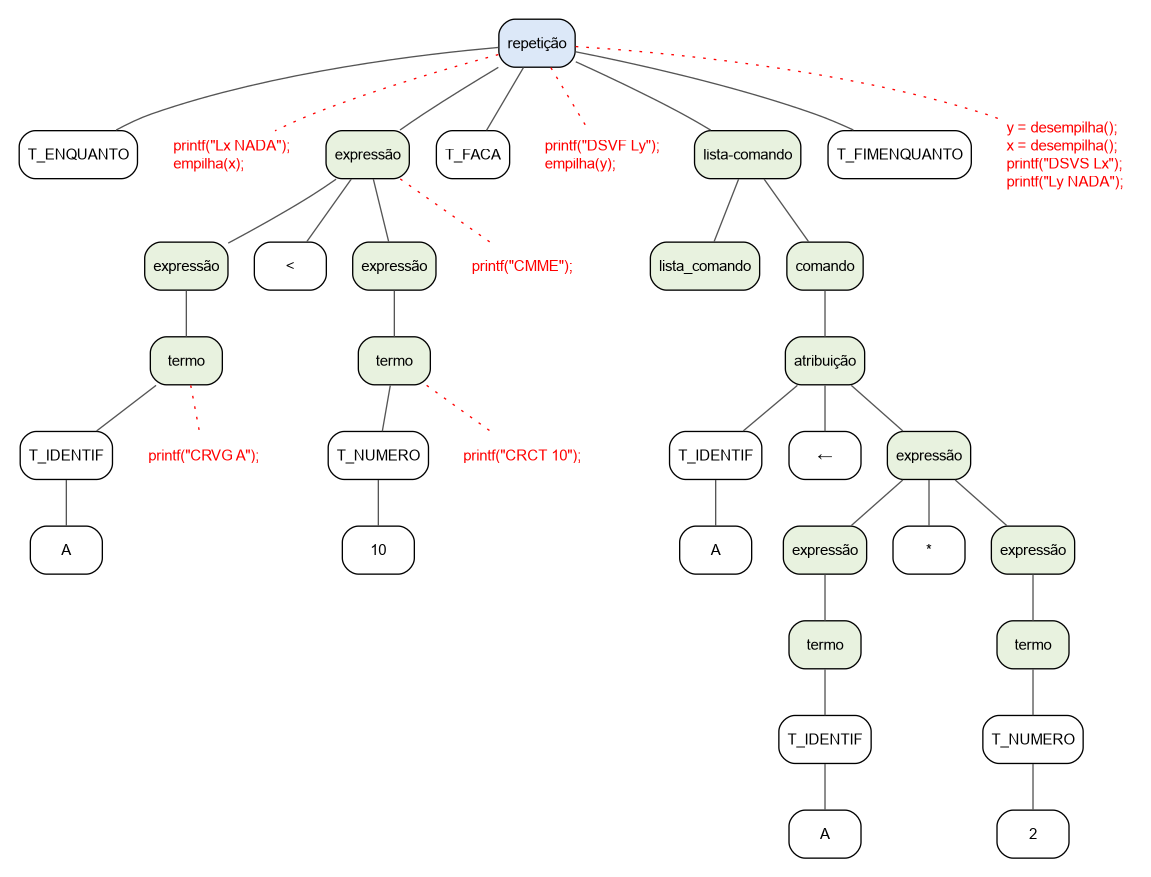
\includegraphics[width=0.9\linewidth,height=\textheight,keepaspectratio]{chapters/images/arvore-repeticao.png}

}

\caption{\label{fig-arvore-repeticao}Árvore de derivação para a
estrutura de repetição}

\end{figure}%

\subsubsection{Comando de seleção}\label{comando-de-seleuxe7uxe3o}

A produção \texttt{selecao} implementa a estrutura condicional
\texttt{se\ ...\ entao\ ...\ senao\ ...\ fimse}.

Após reconhecer a condição, o compilador verifica se ela é lógica. Em
seguida, emite \texttt{DSVF} para desviar para o bloco alternativo caso
a condição seja falsa.

Quando o bloco \texttt{entao} termina, o compilador emite \texttt{DSVS}
para saltar o bloco \texttt{senao} e define o rótulo que marca o início
desse bloco. Finalmente, ao reconhecer \texttt{fimse}, define o rótulo
de encerramento.

Assim, os comandos condicionais são traduzidos por meio de desvios
explícitos, sem exigir que a MVS tenha uma instrução única que
represente toda a estrutura \texttt{se\ ...\ senao}.

A utilização de rótulos permite que o código gerado represente a escolha
entre dois caminhos de execução, preservando o comportamento definido
pelo programa-fonte.

\begin{Shaded}
\begin{Highlighting}[]
\NormalTok{selecao}
    \OperatorTok{:}\NormalTok{ T\_SE expressao T\_ENTAO}
        \OperatorTok{\{} 
            \DataTypeTok{int}\NormalTok{ t }\OperatorTok{=}\NormalTok{ desempilha}\OperatorTok{(}\CharTok{\textquotesingle{}t\textquotesingle{}}\OperatorTok{);}
            \ControlFlowTok{if} \OperatorTok{(}\NormalTok{t }\OperatorTok{!=}\NormalTok{ LOG}\OperatorTok{)}
\NormalTok{                yyerror}\OperatorTok{(}\StringTok{"Incompatibilidade de tipo na condição da seleção"}\OperatorTok{);}
\NormalTok{            fprintf}\OperatorTok{(}\NormalTok{yyout}\OperatorTok{,} \StringTok{"}\SpecialCharTok{\textbackslash{}t}\StringTok{DSVF}\SpecialCharTok{\textbackslash{}t}\StringTok{L}\SpecialCharTok{\%d\textbackslash{}n}\StringTok{"}\OperatorTok{,} \OperatorTok{++}\NormalTok{rotulo}\OperatorTok{);}
\NormalTok{            empilha}\OperatorTok{(}\NormalTok{rotulo}\OperatorTok{,} \CharTok{\textquotesingle{}r\textquotesingle{}}\OperatorTok{);} 
        \OperatorTok{\}} 
\NormalTok{      lista\_comandos T\_SENAO }
        \OperatorTok{\{} 
            \DataTypeTok{int}\NormalTok{ x }\OperatorTok{=}\NormalTok{ desempilha}\OperatorTok{(}\CharTok{\textquotesingle{}r\textquotesingle{}}\OperatorTok{);}
\NormalTok{            fprintf}\OperatorTok{(}\NormalTok{yyout}\OperatorTok{,} \StringTok{"}\SpecialCharTok{\textbackslash{}t}\StringTok{DSVS}\SpecialCharTok{\textbackslash{}t}\StringTok{L}\SpecialCharTok{\%d\textbackslash{}n}\StringTok{"}\OperatorTok{,} \OperatorTok{++}\NormalTok{rotulo}\OperatorTok{);}
\NormalTok{            fprintf}\OperatorTok{(}\NormalTok{yyout}\OperatorTok{,} \StringTok{"L}\SpecialCharTok{\%d\textbackslash{}t}\StringTok{NADA}\SpecialCharTok{\textbackslash{}n}\StringTok{"}\OperatorTok{,}\NormalTok{ x}\OperatorTok{);}
\NormalTok{            empilha}\OperatorTok{(}\NormalTok{rotulo}\OperatorTok{,} \CharTok{\textquotesingle{}r\textquotesingle{}}\OperatorTok{);}
        \OperatorTok{\}}
\NormalTok{      lista\_comandos T\_FIMSE}
        \OperatorTok{\{} 
            \DataTypeTok{int}\NormalTok{ y }\OperatorTok{=}\NormalTok{ desempilha}\OperatorTok{(}\CharTok{\textquotesingle{}r\textquotesingle{}}\OperatorTok{);}
\NormalTok{            fprintf}\OperatorTok{(}\NormalTok{yyout}\OperatorTok{,} \StringTok{"L}\SpecialCharTok{\%d\textbackslash{}t}\StringTok{NADA}\SpecialCharTok{\textbackslash{}n}\StringTok{"}\OperatorTok{,}\NormalTok{ y}\OperatorTok{);} 
        \OperatorTok{\}}
    \OperatorTok{;}
\end{Highlighting}
\end{Shaded}

As ações semânticas incluídas nas regras de derivação para tradução da
estrutura de seleção está representada na
Figura~\ref{fig-arvore-selecao}.

\begin{figure}

\centering{

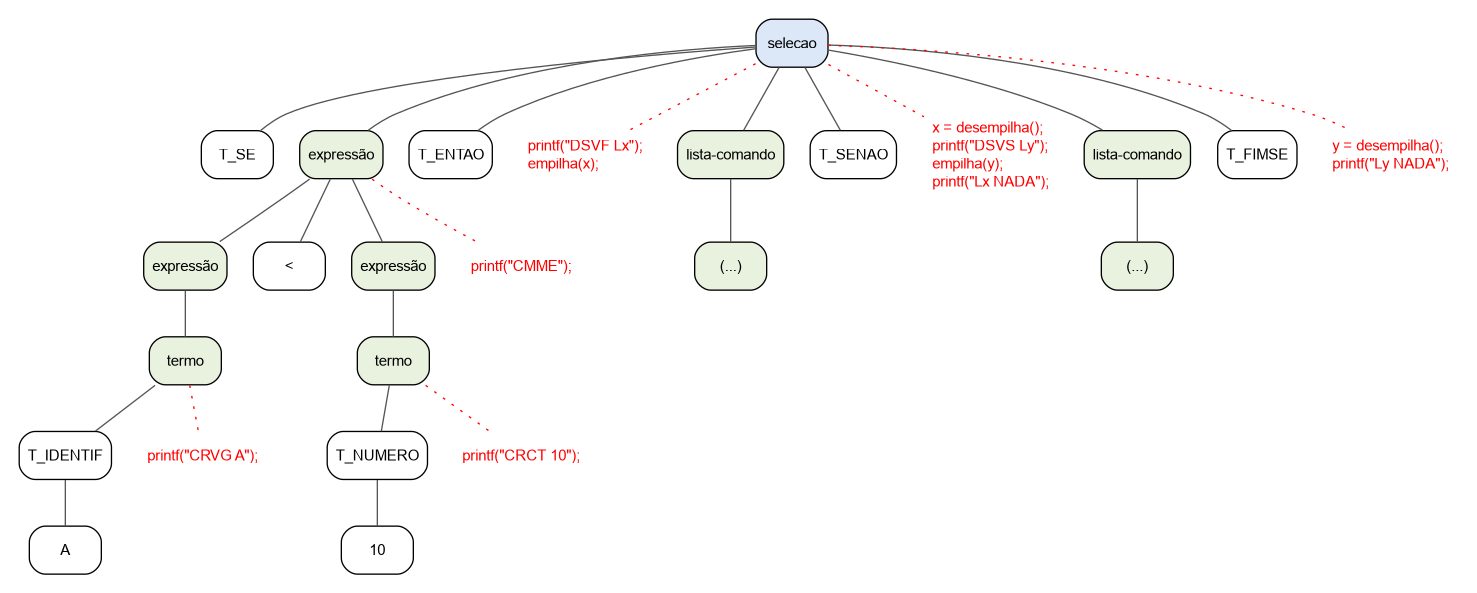
\includegraphics[width=0.9\linewidth,height=\textheight,keepaspectratio]{chapters/images/arvore-selecao.png}

}

\caption{\label{fig-arvore-selecao}Árvore de derivação para a estrutura
de seleção}

\end{figure}%

\subsection{Programa principal e arquivos de entrada e
saída}\label{programa-principal-e-arquivos-de-entrada-e-sauxedda}

Ao final de \texttt{sintatico.y}, a função \texttt{main} controla a
execução do compilador. Ela recebe o nome do arquivo-fonte como
argumento da linha de comando, prepara os nomes dos arquivos de entrada
e saída e chama o analisador sintático.

O compilador espera um arquivo com extensão \texttt{.simples} e produz
um arquivo com extensão \texttt{.mvs}. Por exemplo, ao receber
\texttt{teste.simples}, o programa utiliza \texttt{teste.simples} como
entrada e \texttt{teste.mvs} como saída.

As variáveis \texttt{yyin} e \texttt{yyout} são utilizadas para indicar,
respectivamente, os arquivos lidos e escritos pelo compilador. Depois de
abrir esses arquivos, a função chama \texttt{yyparse()}, que inicia o
reconhecimento sintático. Durante essa análise, as ações semânticas
verificam as declarações e expressões e escrevem as instruções geradas
em \texttt{yyout}.

Ao final, o programa imprime a mensagem \texttt{Programa\ Ok!}. Na
implementação apresentada, essa mensagem é emitida após o retorno de
\texttt{yyparse()}, sem verificar explicitamente seu código de retorno.
Portanto, a mensagem, isoladamente, não constitui uma confirmação
robusta de que toda a compilação ocorreu sem erros.

\subsection{Considerações sobre a
implementação}\label{considerauxe7uxf5es-sobre-a-implementauxe7uxe3o}

A implementação demonstra como a análise semântica e a geração de código
podem ser realizadas de maneira integrada. A tabela de símbolos mantém
as informações sobre os identificadores, a pilha auxiliar acompanha os
tipos das expressões e as ações semânticas produzem diretamente as
instruções da MVS.

Essa abordagem permite estudar a tradução de uma linguagem simples sem
introduzir, inicialmente, todas as etapas de um compilador industrial.
Ao mesmo tempo, evidencia algumas limitações que podem orientar
extensões futuras do projeto.

Entre elas, destacam-se a ampliação das regras de compatibilidade de
tipos, o tratamento de erros com recuperação da análise, a validação
mais rigorosa das condições de execução e a introdução de uma
representação intermediária para separar a análise sintática da geração
de código.

Também é importante observar que os arquivos apresentados não incluem a
implementação do analisador léxico nem a definição completa da MVS. Por
isso, os exemplos de tradução pressupõem que os tokens sejam fornecidos
corretamente e que as instruções emitidas correspondam à semântica
adotada pela máquina virtual.

Com esse projeto, o estudante pode acompanhar concretamente o percurso
de um programa desde o reconhecimento de suas construções sintáticas até
a geração das instruções que serão executadas. O compilador evidencia,
assim, a função da análise semântica na verificação da consistência do
programa e o papel das ações semânticas na tradução das construções da
linguagem de origem para o código da máquina de destino.

\section{Código Completo}\label{cuxf3digo-completo}

\textbf{Arquivo \texttt{makefile}}

\begin{Shaded}
\begin{Highlighting}[]
\NormalTok{simples}\OperatorTok{:}\NormalTok{ utils}\OperatorTok{.}\NormalTok{c lexico}\OperatorTok{.}\NormalTok{l sintatico}\OperatorTok{.}\NormalTok{y }\OperatorTok{;}\NormalTok{\textbackslash{}}
\NormalTok{    flex }\OperatorTok{{-}}\NormalTok{o lexico}\OperatorTok{.}\NormalTok{c lexico}\OperatorTok{.}\NormalTok{l}
\NormalTok{    bison }\OperatorTok{{-}}\NormalTok{o sintatico}\OperatorTok{.}\NormalTok{c sintatico}\OperatorTok{.}\NormalTok{y }\OperatorTok{{-}}\NormalTok{v }\OperatorTok{{-}}\NormalTok{d}
\NormalTok{    gcc sintatico}\OperatorTok{.}\NormalTok{c }\OperatorTok{{-}}\NormalTok{o simples}

\NormalTok{limpa}\OperatorTok{:} \OperatorTok{;}\NormalTok{\textbackslash{}}
\NormalTok{    rm simples lexico}\OperatorTok{.}\NormalTok{c sintatico}\OperatorTok{.}\NormalTok{c sintatico}\OperatorTok{.}\NormalTok{h sintatico}\OperatorTok{.}\NormalTok{output}
\end{Highlighting}
\end{Shaded}

\textbf{Arquivo \texttt{utils.c}}

\begin{Shaded}
\begin{Highlighting}[]
\PreprocessorTok{\#include }\ImportTok{\textless{}stdio.h\textgreater{}}

\KeywordTok{extern} \DataTypeTok{FILE} \OperatorTok{*}\NormalTok{stderr}\OperatorTok{;}
\KeywordTok{extern} \DataTypeTok{int}\NormalTok{ nlinha}\OperatorTok{;}

\DataTypeTok{void}\NormalTok{ yyerror}\OperatorTok{(}\DataTypeTok{const} \DataTypeTok{char} \OperatorTok{*);}

\KeywordTok{enum}
\OperatorTok{\{}
\NormalTok{    INT }\OperatorTok{=} \DecValTok{10}\OperatorTok{,}
\NormalTok{    LOG }\OperatorTok{=} \DecValTok{20}
\OperatorTok{\};}

\CommentTok{/*{-}{-}{-}{-}{-}{-}{-}{-}{-}{-}{-}{-}{-}{-}{-}{-}{-}{-}{-}{-}{-}{-}{-}{-}{-}{-}{-}{-}{-}{-}{-}{-}{-}{-}{-}}
\CommentTok{ * Estrutura da Pilha Semantica}
\CommentTok{ *{-}{-}{-}{-}{-}{-}{-}{-}{-}{-}{-}{-}{-}{-}{-}{-}{-}{-}{-}{-}{-}{-}{-}{-}{-}{-}{-}{-}{-}{-}{-}{-}{-}{-}{-}*/}
\PreprocessorTok{\#define TAMPILHA }\DecValTok{100}
\KeywordTok{struct}
\OperatorTok{\{}
    \DataTypeTok{int}\NormalTok{ valor}\OperatorTok{;}
    \DataTypeTok{char}\NormalTok{ tipo}\OperatorTok{;}
\OperatorTok{\}}\NormalTok{ Pilha}\OperatorTok{[}\NormalTok{TAMPILHA}\OperatorTok{];}

\DataTypeTok{int}\NormalTok{ topo }\OperatorTok{=} \OperatorTok{{-}}\DecValTok{1}\OperatorTok{;}

\DataTypeTok{void}\NormalTok{ empilha}\OperatorTok{(}\DataTypeTok{int}\NormalTok{ valor}\OperatorTok{,} \DataTypeTok{char}\NormalTok{ tipo}\OperatorTok{)}
\OperatorTok{\{}
    \ControlFlowTok{if} \OperatorTok{(}\NormalTok{topo }\OperatorTok{\textgreater{}}\NormalTok{ TAMPILHA}\OperatorTok{)}
\NormalTok{        yyerror}\OperatorTok{(}\StringTok{"Pilha Cheia"}\OperatorTok{);}
\NormalTok{    Pilha}\OperatorTok{[++}\NormalTok{topo}\OperatorTok{].}\NormalTok{valor }\OperatorTok{=}\NormalTok{ valor}\OperatorTok{;}
\NormalTok{    Pilha}\OperatorTok{[}\NormalTok{topo}\OperatorTok{].}\NormalTok{tipo }\OperatorTok{=}\NormalTok{ tipo}\OperatorTok{;}
\OperatorTok{\}}

\DataTypeTok{int}\NormalTok{ desempilha}\OperatorTok{(}\DataTypeTok{char}\NormalTok{ tipo}\OperatorTok{)}
\OperatorTok{\{}
    \ControlFlowTok{if} \OperatorTok{(}\NormalTok{topo }\OperatorTok{==} \OperatorTok{{-}}\DecValTok{1}\OperatorTok{)}
\NormalTok{        yyerror}\OperatorTok{(}\StringTok{"Pilha Vazia"}\OperatorTok{);}
    \ControlFlowTok{if} \OperatorTok{(}\NormalTok{Pilha}\OperatorTok{[}\NormalTok{topo}\OperatorTok{].}\NormalTok{tipo }\OperatorTok{!=}\NormalTok{ tipo}\OperatorTok{)}
\NormalTok{        yyerror}\OperatorTok{(}\StringTok{"Tipo diferente no desempilha"}\OperatorTok{);}
    \ControlFlowTok{return}\NormalTok{ Pilha}\OperatorTok{[}\NormalTok{topo}\OperatorTok{{-}{-}].}\NormalTok{valor}\OperatorTok{;}
\OperatorTok{\}}

\DataTypeTok{void}\NormalTok{ testatipo}\OperatorTok{(}\DataTypeTok{int}\NormalTok{ tipo1}\OperatorTok{,} \DataTypeTok{int}\NormalTok{ tipo2}\OperatorTok{,} \DataTypeTok{int}\NormalTok{ ret}\OperatorTok{)}
\OperatorTok{\{}
    \DataTypeTok{int}\NormalTok{ t2 }\OperatorTok{=}\NormalTok{ desempilha}\OperatorTok{(}\CharTok{\textquotesingle{}t\textquotesingle{}}\OperatorTok{);}
    \DataTypeTok{int}\NormalTok{ t1 }\OperatorTok{=}\NormalTok{ desempilha}\OperatorTok{(}\CharTok{\textquotesingle{}t\textquotesingle{}}\OperatorTok{);}

    \ControlFlowTok{if} \OperatorTok{(}\NormalTok{t1 }\OperatorTok{!=}\NormalTok{ tipo1 }\OperatorTok{||}\NormalTok{ t2 }\OperatorTok{!=}\NormalTok{ tipo2}\OperatorTok{)}
\NormalTok{        yyerror}\OperatorTok{(}\StringTok{"Incompatibilidade de tipo!"}\OperatorTok{);}

\NormalTok{    empilha}\OperatorTok{(}\NormalTok{ret}\OperatorTok{,} \CharTok{\textquotesingle{}t\textquotesingle{}}\OperatorTok{);}
\OperatorTok{\}}

\DataTypeTok{void}\NormalTok{ mostrapilha}\OperatorTok{()}
\OperatorTok{\{}
\NormalTok{    printf}\OperatorTok{(}\StringTok{"Pilha = ["}\OperatorTok{);}
    \ControlFlowTok{for} \OperatorTok{(}\DataTypeTok{int}\NormalTok{ i }\OperatorTok{=}\NormalTok{ topo}\OperatorTok{;}\NormalTok{ i }\OperatorTok{\textgreater{}=} \DecValTok{0}\OperatorTok{;}\NormalTok{ i}\OperatorTok{{-}{-})}
\NormalTok{        printf}\OperatorTok{(}\StringTok{"(}\SpecialCharTok{\%d}\StringTok{,}\SpecialCharTok{\%c}\StringTok{) "}\OperatorTok{,}\NormalTok{ Pilha}\OperatorTok{[}\NormalTok{i}\OperatorTok{].}\NormalTok{valor}\OperatorTok{,}\NormalTok{ Pilha}\OperatorTok{[}\NormalTok{i}\OperatorTok{].}\NormalTok{tipo}\OperatorTok{);}
\NormalTok{    printf}\OperatorTok{(}\StringTok{"]}\SpecialCharTok{\textbackslash{}n}\StringTok{"}\OperatorTok{);}
\OperatorTok{\}}

\CommentTok{/*{-}{-}{-}{-}{-}{-}{-}{-}{-}{-}{-}{-}{-}{-}{-}{-}{-}{-}{-}{-}{-}{-}{-}{-}{-}{-}{-}{-}{-}{-}{-}{-}{-}{-}{-}}
\CommentTok{ * Estrutura da Tabela de Símbolos}
\CommentTok{ *{-}{-}{-}{-}{-}{-}{-}{-}{-}{-}{-}{-}{-}{-}{-}{-}{-}{-}{-}{-}{-}{-}{-}{-}{-}{-}{-}{-}{-}{-}{-}{-}{-}{-}{-}*/}

\PreprocessorTok{\#define TAMTAB }\DecValTok{100}
\KeywordTok{typedef} \KeywordTok{struct}
\OperatorTok{\{}
    \DataTypeTok{char}\NormalTok{ nome}\OperatorTok{[}\DecValTok{30}\OperatorTok{];}
    \DataTypeTok{int}\NormalTok{ tipo}\OperatorTok{;}
    \DataTypeTok{int}\NormalTok{ end}\OperatorTok{;}
\OperatorTok{\}}\NormalTok{ tiptab}\OperatorTok{;}

\NormalTok{tiptab elemtab}\OperatorTok{,}\NormalTok{ tabsimb}\OperatorTok{[}\NormalTok{TAMTAB}\OperatorTok{];}
\DataTypeTok{int}\NormalTok{ topotab }\OperatorTok{=} \OperatorTok{{-}}\DecValTok{1}\OperatorTok{;}

\DataTypeTok{void}\NormalTok{ inseresimbolo}\OperatorTok{(}\NormalTok{tiptab elem}\OperatorTok{)}
\OperatorTok{\{}
    \DataTypeTok{int}\NormalTok{ i}\OperatorTok{;}
    \ControlFlowTok{for} \OperatorTok{(}\NormalTok{i }\OperatorTok{=}\NormalTok{ topotab}\OperatorTok{;}\NormalTok{ i }\OperatorTok{\textgreater{}=} \DecValTok{0} \OperatorTok{\&\&}\NormalTok{ strcmp}\OperatorTok{(}\NormalTok{elem}\OperatorTok{.}\NormalTok{nome}\OperatorTok{,}\NormalTok{ tabsimb}\OperatorTok{[}\NormalTok{i}\OperatorTok{].}\NormalTok{nome}\OperatorTok{)} \OperatorTok{!=} \DecValTok{0}\OperatorTok{;}\NormalTok{ i}\OperatorTok{{-}{-})}
        \OperatorTok{;}
    \ControlFlowTok{if} \OperatorTok{(}\NormalTok{i }\OperatorTok{!=} \OperatorTok{{-}}\DecValTok{1}\OperatorTok{)}
    \OperatorTok{\{}
\NormalTok{        yyerror}\OperatorTok{(}\StringTok{"Identificador duplicado"}\OperatorTok{);}
    \OperatorTok{\}}
\NormalTok{    tabsimb}\OperatorTok{[++}\NormalTok{topotab}\OperatorTok{]} \OperatorTok{=}\NormalTok{ elem}\OperatorTok{;}
\OperatorTok{\}}

\DataTypeTok{int}\NormalTok{ buscasimbolo}\OperatorTok{(}\DataTypeTok{char} \OperatorTok{*}\NormalTok{nome}\OperatorTok{)}
\OperatorTok{\{}
    \DataTypeTok{int}\NormalTok{ i}\OperatorTok{;}
    \ControlFlowTok{for} \OperatorTok{(}\NormalTok{i }\OperatorTok{=}\NormalTok{ topotab}\OperatorTok{;}\NormalTok{ i }\OperatorTok{\textgreater{}=} \DecValTok{0} \OperatorTok{\&\&}\NormalTok{ strcmp}\OperatorTok{(}\NormalTok{nome}\OperatorTok{,}\NormalTok{ tabsimb}\OperatorTok{[}\NormalTok{i}\OperatorTok{].}\NormalTok{nome}\OperatorTok{)} \OperatorTok{!=} \DecValTok{0}\OperatorTok{;}\NormalTok{ i}\OperatorTok{{-}{-})}
        \OperatorTok{;}
    \ControlFlowTok{if} \OperatorTok{(}\NormalTok{i }\OperatorTok{==} \OperatorTok{{-}}\DecValTok{1}\OperatorTok{)}
    \OperatorTok{\{}
\NormalTok{        yyerror}\OperatorTok{(}\StringTok{"Identificador não encontrado"}\OperatorTok{);}
    \OperatorTok{\}}
    \ControlFlowTok{return}\NormalTok{ i}\OperatorTok{;}
\OperatorTok{\}}

\DataTypeTok{void}\NormalTok{ mostratabela}\OperatorTok{()}
\OperatorTok{\{}
\NormalTok{    printf}\OperatorTok{(}\StringTok{"}\SpecialCharTok{\%10s}\StringTok{ }\SpecialCharTok{\%3s}\StringTok{ }\SpecialCharTok{\%3s\textbackslash{}n}\StringTok{"}\OperatorTok{,} \StringTok{"Nome"}\OperatorTok{,} \StringTok{"Tipo"}\OperatorTok{,} \StringTok{"End"}\OperatorTok{);}
    \ControlFlowTok{for} \OperatorTok{(}\DataTypeTok{int}\NormalTok{ i }\OperatorTok{=} \DecValTok{0}\OperatorTok{;}\NormalTok{ i }\OperatorTok{\textless{}=}\NormalTok{ topotab}\OperatorTok{;}\NormalTok{ i}\OperatorTok{++)}
    \OperatorTok{\{}
\NormalTok{        printf}\OperatorTok{(}\StringTok{"}\SpecialCharTok{\%10s}\StringTok{ }\SpecialCharTok{\%3d}\StringTok{ }\SpecialCharTok{\%3d\textbackslash{}n}\StringTok{"}\OperatorTok{,} 
\NormalTok{             tabsimb}\OperatorTok{[}\NormalTok{i}\OperatorTok{].}\NormalTok{nome}\OperatorTok{,}\NormalTok{ tabsimb}\OperatorTok{[}\NormalTok{i}\OperatorTok{].}\NormalTok{tipo}\OperatorTok{,}\NormalTok{ tabsimb}\OperatorTok{[}\NormalTok{i}\OperatorTok{].}\NormalTok{end}\OperatorTok{);}
    \OperatorTok{\}}
\OperatorTok{\}}
\end{Highlighting}
\end{Shaded}

\textbf{Arquivo \texttt{lexico.l}}

\begin{Shaded}
\begin{Highlighting}[]
\OperatorTok{\%\{}
\PreprocessorTok{\#include }\ImportTok{"sintatico.h"}
\DataTypeTok{int}\NormalTok{ nlinha }\OperatorTok{=} \DecValTok{1}\OperatorTok{;}
\DataTypeTok{char}\NormalTok{ atomo}\OperatorTok{[}\DecValTok{30}\OperatorTok{];}
\DataTypeTok{void}\NormalTok{ yyerror}\OperatorTok{(}\DataTypeTok{const} \DataTypeTok{char} \OperatorTok{*);}

\OperatorTok{\%\}}

\NormalTok{identificador }\OperatorTok{[}\NormalTok{a}\OperatorTok{{-}}\NormalTok{zA}\OperatorTok{{-}}\NormalTok{Z}\OperatorTok{]([}\NormalTok{a}\OperatorTok{{-}}\NormalTok{zA}\OperatorTok{{-}}\NormalTok{Z}\OperatorTok{]|[}\DecValTok{0}\OperatorTok{{-}}\DecValTok{9}\OperatorTok{])*}
\NormalTok{numero }\OperatorTok{[}\DecValTok{0}\OperatorTok{{-}}\DecValTok{9}\OperatorTok{]+}
\NormalTok{espaco }\OperatorTok{[}\NormalTok{ \textbackslash{}t}\OperatorTok{]+}
\NormalTok{novalinha }\OperatorTok{[}\NormalTok{\textbackslash{}n}\OperatorTok{]}

\OperatorTok{\%\%}
\NormalTok{programa          }\OperatorTok{\{} \ControlFlowTok{return}\NormalTok{ T\_PROG}\OperatorTok{;} \OperatorTok{\}}
\NormalTok{inicio            }\OperatorTok{\{} \ControlFlowTok{return}\NormalTok{ T\_INICIO}\OperatorTok{;} \OperatorTok{\}}
\NormalTok{fimprograma       }\OperatorTok{\{} \ControlFlowTok{return}\NormalTok{ T\_FIM}\OperatorTok{;} \OperatorTok{\}}
\NormalTok{leia              }\OperatorTok{\{} \ControlFlowTok{return}\NormalTok{ T\_LEIA}\OperatorTok{;} \OperatorTok{\}}
\NormalTok{escreva           }\OperatorTok{\{} \ControlFlowTok{return}\NormalTok{ T\_ESCREVA}\OperatorTok{;} \OperatorTok{\}}
\NormalTok{se                }\OperatorTok{\{} \ControlFlowTok{return}\NormalTok{ T\_SE}\OperatorTok{;} \OperatorTok{\}}
\NormalTok{entao             }\OperatorTok{\{} \ControlFlowTok{return}\NormalTok{ T\_ENTAO}\OperatorTok{;} \OperatorTok{\}}
\NormalTok{senao             }\OperatorTok{\{} \ControlFlowTok{return}\NormalTok{ T\_SENAO}\OperatorTok{;} \OperatorTok{\}}
\NormalTok{fimse             }\OperatorTok{\{} \ControlFlowTok{return}\NormalTok{ T\_FIMSE}\OperatorTok{;} \OperatorTok{\}}
\NormalTok{enquanto          }\OperatorTok{\{} \ControlFlowTok{return}\NormalTok{ T\_ENQTO}\OperatorTok{;} \OperatorTok{\}}
\NormalTok{faca              }\OperatorTok{\{} \ControlFlowTok{return}\NormalTok{ T\_FACA}\OperatorTok{;} \OperatorTok{\}}
\NormalTok{fimenquanto       }\OperatorTok{\{} \ControlFlowTok{return}\NormalTok{ T\_FIMENQTO}\OperatorTok{;} \OperatorTok{\}}

\NormalTok{inteiro           }\OperatorTok{\{} \ControlFlowTok{return}\NormalTok{ T\_INTEIRO}\OperatorTok{;} \OperatorTok{\}}
\NormalTok{logico            }\OperatorTok{\{} \ControlFlowTok{return}\NormalTok{ T\_LOGICO}\OperatorTok{;} \OperatorTok{\}}

\NormalTok{V                 }\OperatorTok{\{} \ControlFlowTok{return}\NormalTok{ T\_V}\OperatorTok{;} \OperatorTok{\}}
\NormalTok{F                 }\OperatorTok{\{} \ControlFlowTok{return}\NormalTok{ T\_F}\OperatorTok{;} \OperatorTok{\}}

\StringTok{"+"}               \OperatorTok{\{} \ControlFlowTok{return}\NormalTok{ T\_MAIS}\OperatorTok{;} \OperatorTok{\}}
\StringTok{"{-}"}               \OperatorTok{\{} \ControlFlowTok{return}\NormalTok{ T\_MENOS}\OperatorTok{;} \OperatorTok{\}}
\StringTok{"*"}               \OperatorTok{\{} \ControlFlowTok{return}\NormalTok{ T\_VEZES}\OperatorTok{;} \OperatorTok{\}}
\NormalTok{div               }\OperatorTok{\{} \ControlFlowTok{return}\NormalTok{ T\_DIV}\OperatorTok{;} \OperatorTok{\}}
\StringTok{"\textgreater{}"}               \OperatorTok{\{} \ControlFlowTok{return}\NormalTok{ T\_MAIOR}\OperatorTok{;} \OperatorTok{\}}
\StringTok{"\textless{}"}               \OperatorTok{\{} \ControlFlowTok{return}\NormalTok{ T\_MENOR}\OperatorTok{;} \OperatorTok{\}}
\StringTok{"="}               \OperatorTok{\{} \ControlFlowTok{return}\NormalTok{ T\_IGUAL}\OperatorTok{;} \OperatorTok{\}}
\NormalTok{E                 }\OperatorTok{\{} \ControlFlowTok{return}\NormalTok{ T\_E}\OperatorTok{;} \OperatorTok{\}}
\NormalTok{OU                }\OperatorTok{\{} \ControlFlowTok{return}\NormalTok{ T\_OU}\OperatorTok{;} \OperatorTok{\}}
\NormalTok{NAO               }\OperatorTok{\{} \ControlFlowTok{return}\NormalTok{ T\_NAO}\OperatorTok{;} \OperatorTok{\}}
\StringTok{"\textless{}{-}"}              \OperatorTok{\{} \ControlFlowTok{return}\NormalTok{ T\_ATRIB}\OperatorTok{;} \OperatorTok{\}}
\StringTok{"("}               \OperatorTok{\{} \ControlFlowTok{return}\NormalTok{ T\_ABRE}\OperatorTok{;\}}
\StringTok{")"}               \OperatorTok{\{} \ControlFlowTok{return}\NormalTok{ T\_FECHA}\OperatorTok{;} \OperatorTok{\}}

\OperatorTok{\{}\NormalTok{identificador}\OperatorTok{\}}   \OperatorTok{\{} 
\NormalTok{                     strcpy}\OperatorTok{(}\NormalTok{atomo}\OperatorTok{,}\NormalTok{ yytext}\OperatorTok{);}
                     \ControlFlowTok{return}\NormalTok{ T\_IDENTIF}\OperatorTok{;} 
                  \OperatorTok{\}}
\OperatorTok{\{}\NormalTok{numero}\OperatorTok{\}}          \OperatorTok{\{} 
\NormalTok{                     strcpy}\OperatorTok{(}\NormalTok{atomo}\OperatorTok{,}\NormalTok{ yytext}\OperatorTok{);}
                     \ControlFlowTok{return}\NormalTok{ T\_NUMERO}\OperatorTok{;} 
                  \OperatorTok{\}}
\OperatorTok{\{}\NormalTok{espaco}\OperatorTok{\}}          \OperatorTok{\{}  \OperatorTok{\}}
\OperatorTok{\{}\NormalTok{novalinha}\OperatorTok{\}}       \OperatorTok{\{}\NormalTok{  nlinha}\OperatorTok{++;} \OperatorTok{\}}

\OperatorTok{.}                 \OperatorTok{\{} 
                      \DataTypeTok{char}\NormalTok{ msg}\OperatorTok{[}\DecValTok{100}\OperatorTok{];}
\NormalTok{                      sprintf}\OperatorTok{(}\NormalTok{msg}\OperatorTok{,} \StringTok{"  símbolo }\SpecialCharTok{\%s}\StringTok{ desconhecido!"}\OperatorTok{,}\NormalTok{ yytext}\OperatorTok{);}
\NormalTok{                      yyerror}\OperatorTok{(}\NormalTok{msg}\OperatorTok{);} 
                  \OperatorTok{\}}
\OperatorTok{\%\%}


\DataTypeTok{int}\NormalTok{ yywrap}\OperatorTok{()} \OperatorTok{\{}
  \ControlFlowTok{return} \DecValTok{1}\OperatorTok{;}
\OperatorTok{\}}
\end{Highlighting}
\end{Shaded}

\textbf{Arquivo \texttt{sintatico.y}}

\begin{Shaded}
\begin{Highlighting}[]
\OperatorTok{\%\{}
\PreprocessorTok{\#include }\ImportTok{\textless{}stdio.h\textgreater{}}
\PreprocessorTok{\#include }\ImportTok{\textless{}stdlib.h\textgreater{}}
\PreprocessorTok{\#include }\ImportTok{\textless{}string.h\textgreater{}}
\PreprocessorTok{\#include }\ImportTok{"lexico.c"}
\PreprocessorTok{\#include }\ImportTok{"utils.c"}

\KeywordTok{extern} \DataTypeTok{FILE} \OperatorTok{*}\NormalTok{yyin}\OperatorTok{;}   \CommentTok{// arquivo de entrada (.simples)}
\KeywordTok{extern} \DataTypeTok{FILE} \OperatorTok{*}\NormalTok{yyout}\OperatorTok{;}  \CommentTok{// arquivo de saida (.mvs)}
\KeywordTok{extern} \DataTypeTok{int}\NormalTok{ nlinha}\OperatorTok{;}   \CommentTok{// numero da linha}
\DataTypeTok{int}\NormalTok{ contavar }\OperatorTok{=} \DecValTok{0}\OperatorTok{;}    \CommentTok{// contador de variveis}
\DataTypeTok{int}\NormalTok{ rotulo }\OperatorTok{=} \DecValTok{0}\OperatorTok{;}      \CommentTok{// contador de rotulos}
\DataTypeTok{int}\NormalTok{ tipo}\OperatorTok{;}            \CommentTok{// tipo da variavel}
\PreprocessorTok{\#define DEBUG}\OperatorTok{(}\PreprocessorTok{x}\OperatorTok{)}\PreprocessorTok{ }

\OperatorTok{\%\}}

\OperatorTok{\%}\NormalTok{token T\_PROG}
\OperatorTok{\%}\NormalTok{token T\_INICIO}
\OperatorTok{\%}\NormalTok{token T\_FIM}
\OperatorTok{\%}\NormalTok{token T\_IDENTIF}
\OperatorTok{\%}\NormalTok{token T\_LEIA}
\OperatorTok{\%}\NormalTok{token T\_ESCREVA}
\OperatorTok{\%}\NormalTok{token T\_ENQTO}
\OperatorTok{\%}\NormalTok{token T\_FACA}
\OperatorTok{\%}\NormalTok{token T\_FIMENQTO}
\OperatorTok{\%}\NormalTok{token T\_SE }
\OperatorTok{\%}\NormalTok{token T\_ENTAO}
\OperatorTok{\%}\NormalTok{token T\_SENAO}
\OperatorTok{\%}\NormalTok{token T\_FIMSE}
\OperatorTok{\%}\NormalTok{token T\_ATRIB}
\OperatorTok{\%}\NormalTok{token T\_VEZES}
\OperatorTok{\%}\NormalTok{token T\_DIV}
\OperatorTok{\%}\NormalTok{token T\_MAIS}
\OperatorTok{\%}\NormalTok{token T\_MENOS}
\OperatorTok{\%}\NormalTok{token T\_MAIOR}
\OperatorTok{\%}\NormalTok{token T\_MENOR}
\OperatorTok{\%}\NormalTok{token T\_IGUAL}
\OperatorTok{\%}\NormalTok{token T\_E }
\OperatorTok{\%}\NormalTok{token T\_OU}
\OperatorTok{\%}\NormalTok{token T\_V }
\OperatorTok{\%}\NormalTok{token T\_F }
\OperatorTok{\%}\NormalTok{token T\_NUMERO}
\OperatorTok{\%}\NormalTok{token T\_NAO }
\OperatorTok{\%}\NormalTok{token T\_ABRE}
\OperatorTok{\%}\NormalTok{token T\_FECHA}
\OperatorTok{\%}\NormalTok{token T\_LOGICO}
\OperatorTok{\%}\NormalTok{token T\_INTEIRO}

\OperatorTok{\%}\NormalTok{define parse}\OperatorTok{.}\NormalTok{error custom}

\OperatorTok{\%}\NormalTok{left T\_E T\_OU}
\OperatorTok{\%}\NormalTok{left T\_IGUAL}
\OperatorTok{\%}\NormalTok{left T\_MAIOR T\_MENOR}
\OperatorTok{\%}\NormalTok{left T\_MAIS T\_MENOS}
\OperatorTok{\%}\NormalTok{left T\_VEZES T\_DIV}

\OperatorTok{\%\%}
\NormalTok{programa}
    \OperatorTok{:}\NormalTok{ cabecalho }
         \OperatorTok{\{}\NormalTok{ fprintf}\OperatorTok{(}\NormalTok{yyout}\OperatorTok{,} \StringTok{"}\SpecialCharTok{\textbackslash{}t}\StringTok{INPP}\SpecialCharTok{\textbackslash{}n}\StringTok{"}\OperatorTok{);} \OperatorTok{\}}
\NormalTok{      variaveis }
         \OperatorTok{\{} 
\NormalTok{            DEBUG}\OperatorTok{(}\NormalTok{mostratabela}\OperatorTok{();)}
\NormalTok{            empilha}\OperatorTok{(}\NormalTok{contavar}\OperatorTok{,} \CharTok{\textquotesingle{}c\textquotesingle{}}\OperatorTok{);}
            \ControlFlowTok{if} \OperatorTok{(}\NormalTok{contavar }\OperatorTok{\textgreater{}} \DecValTok{0}\OperatorTok{)} \OperatorTok{\{}
\NormalTok{               fprintf}\OperatorTok{(}\NormalTok{yyout}\OperatorTok{,} \StringTok{"}\SpecialCharTok{\textbackslash{}t}\StringTok{AMEM}\SpecialCharTok{\textbackslash{}t\%d\textbackslash{}n}\StringTok{"}\OperatorTok{,}\NormalTok{ contavar}\OperatorTok{);}
            \OperatorTok{\}} 
         \OperatorTok{\}}
\NormalTok{      T\_INICIO lista\_comandos T\_FIM}
         \OperatorTok{\{}
            \DataTypeTok{int}\NormalTok{ conta }\OperatorTok{=}\NormalTok{ desempilha}\OperatorTok{(}\CharTok{\textquotesingle{}c\textquotesingle{}}\OperatorTok{);}
            \ControlFlowTok{if} \OperatorTok{(}\NormalTok{conta }\OperatorTok{\textgreater{}} \DecValTok{0}\OperatorTok{)} 
\NormalTok{               fprintf}\OperatorTok{(}\NormalTok{yyout}\OperatorTok{,} \StringTok{"}\SpecialCharTok{\textbackslash{}t}\StringTok{DMEM}\SpecialCharTok{\textbackslash{}t\%d\textbackslash{}n}\StringTok{"}\OperatorTok{,}\NormalTok{ conta}\OperatorTok{);}
\NormalTok{            fprintf}\OperatorTok{(}\NormalTok{yyout}\OperatorTok{,} \StringTok{"}\SpecialCharTok{\textbackslash{}t}\StringTok{FIMP}\SpecialCharTok{\textbackslash{}n}\StringTok{"}\OperatorTok{);} 
         \OperatorTok{\}}
    \OperatorTok{;}

\NormalTok{cabecalho}
    \OperatorTok{:}\NormalTok{ T\_PROG T\_IDENTIF}
    \OperatorTok{;}

\NormalTok{variaveis}
    \OperatorTok{:} \CommentTok{/* vazio */}
    \OperatorTok{|}\NormalTok{ declaracao\_variaveis}
    \OperatorTok{;}

\NormalTok{declaracao\_variaveis}
    \OperatorTok{:}\NormalTok{ tipo lista\_variaveis declaracao\_variaveis}
    \OperatorTok{|}\NormalTok{ tipo lista\_variaveis}
    \OperatorTok{;}

\NormalTok{tipo}
    \OperatorTok{:}\NormalTok{ T\_LOGICO}
      \OperatorTok{\{}\NormalTok{ tipo }\OperatorTok{=}\NormalTok{ LOG}\OperatorTok{;} \OperatorTok{\}}
    \OperatorTok{|}\NormalTok{ T\_INTEIRO}
      \OperatorTok{\{}\NormalTok{ tipo }\OperatorTok{=}\NormalTok{ INT}\OperatorTok{;} \OperatorTok{\}}
    \OperatorTok{;}

\NormalTok{lista\_variaveis}
    \OperatorTok{:}\NormalTok{ lista\_variaveis T\_IDENTIF}
      \OperatorTok{\{} 
\NormalTok{        strcpy}\OperatorTok{(}\NormalTok{elemtab}\OperatorTok{.}\NormalTok{nome}\OperatorTok{,}\NormalTok{ atomo}\OperatorTok{);}
\NormalTok{        elemtab}\OperatorTok{.}\NormalTok{tipo }\OperatorTok{=}\NormalTok{ tipo}\OperatorTok{;}
\NormalTok{        elemtab}\OperatorTok{.}\NormalTok{end }\OperatorTok{=}\NormalTok{ contavar}\OperatorTok{;}
\NormalTok{        inseresimbolo}\OperatorTok{(}\NormalTok{elemtab}\OperatorTok{);}
\NormalTok{        contavar}\OperatorTok{++;} 
      \OperatorTok{\}}
    \OperatorTok{|}\NormalTok{ T\_IDENTIF}
      \OperatorTok{\{} 
\NormalTok{        strcpy}\OperatorTok{(}\NormalTok{elemtab}\OperatorTok{.}\NormalTok{nome}\OperatorTok{,}\NormalTok{ atomo}\OperatorTok{);}
\NormalTok{        elemtab}\OperatorTok{.}\NormalTok{tipo }\OperatorTok{=}\NormalTok{ tipo}\OperatorTok{;}
\NormalTok{        elemtab}\OperatorTok{.}\NormalTok{end }\OperatorTok{=}\NormalTok{ contavar}\OperatorTok{;}
\NormalTok{        inseresimbolo}\OperatorTok{(}\NormalTok{elemtab}\OperatorTok{);}
\NormalTok{        contavar}\OperatorTok{++;} 
      \OperatorTok{\}}
    \OperatorTok{;}

\NormalTok{lista\_comandos}
    \OperatorTok{:} \CommentTok{/* vazio */}
    \OperatorTok{|}\NormalTok{ comando lista\_comandos}
    \OperatorTok{;}

\NormalTok{comando}
    \OperatorTok{:}\NormalTok{ leitura}
    \OperatorTok{|}\NormalTok{ escrita}
    \OperatorTok{|}\NormalTok{ repeticao}
    \OperatorTok{|}\NormalTok{ selecao}
    \OperatorTok{|}\NormalTok{ atribuicao}
    \OperatorTok{;}

\NormalTok{leitura}
    \OperatorTok{:}\NormalTok{ T\_LEIA T\_IDENTIF}
       \OperatorTok{\{}
        \DataTypeTok{int}\NormalTok{ pos }\OperatorTok{=}\NormalTok{ buscasimbolo}\OperatorTok{(}\NormalTok{atomo}\OperatorTok{);} 
\NormalTok{        fprintf}\OperatorTok{(}\NormalTok{yyout}\OperatorTok{,}\StringTok{"}\SpecialCharTok{\textbackslash{}t}\StringTok{LEIA}\SpecialCharTok{\textbackslash{}n}\StringTok{"}\OperatorTok{);}
\NormalTok{        fprintf}\OperatorTok{(}\NormalTok{yyout}\OperatorTok{,}\StringTok{"}\SpecialCharTok{\textbackslash{}t}\StringTok{ARZG}\SpecialCharTok{\textbackslash{}t\%d\textbackslash{}n}\StringTok{"}\OperatorTok{,}\NormalTok{ tabsimb}\OperatorTok{[}\NormalTok{pos}\OperatorTok{].}\NormalTok{end}\OperatorTok{);} 
       \OperatorTok{\}}
    \OperatorTok{;}

\NormalTok{escrita}
    \OperatorTok{:}\NormalTok{ T\_ESCREVA expressao}
       \OperatorTok{\{}
        \DataTypeTok{int}\NormalTok{ t }\OperatorTok{=}\NormalTok{ desempilha}\OperatorTok{(}\CharTok{\textquotesingle{}t\textquotesingle{}}\OperatorTok{);} 
\NormalTok{        fprintf}\OperatorTok{(}\NormalTok{yyout}\OperatorTok{,} \StringTok{"}\SpecialCharTok{\textbackslash{}t}\StringTok{ESCR}\SpecialCharTok{\textbackslash{}n}\StringTok{"}\OperatorTok{);} 
       \OperatorTok{\}}
    \OperatorTok{;}

\NormalTok{repeticao}
    \OperatorTok{:}\NormalTok{ T\_ENQTO }
        \OperatorTok{\{} 
\NormalTok{            fprintf}\OperatorTok{(}\NormalTok{yyout}\OperatorTok{,} \StringTok{"L}\SpecialCharTok{\%d\textbackslash{}t}\StringTok{NADA}\SpecialCharTok{\textbackslash{}n}\StringTok{"}\OperatorTok{,} \OperatorTok{++}\NormalTok{rotulo}\OperatorTok{);}
\NormalTok{            empilha}\OperatorTok{(}\NormalTok{rotulo}\OperatorTok{,} \CharTok{\textquotesingle{}r\textquotesingle{}}\OperatorTok{);} 
        \OperatorTok{\}}
\NormalTok{      expressao }
\NormalTok{      T\_FACA }
        \OperatorTok{\{} 
            \DataTypeTok{int}\NormalTok{ t }\OperatorTok{=}\NormalTok{ desempilha}\OperatorTok{(}\CharTok{\textquotesingle{}t\textquotesingle{}}\OperatorTok{);}
            \ControlFlowTok{if} \OperatorTok{(}\NormalTok{t }\OperatorTok{!=}\NormalTok{ LOG}\OperatorTok{)}
\NormalTok{                yyerror}\OperatorTok{(}\StringTok{"Incompatibilidade de tipo na repetição"}\OperatorTok{);}
\NormalTok{            fprintf}\OperatorTok{(}\NormalTok{yyout}\OperatorTok{,} \StringTok{"}\SpecialCharTok{\textbackslash{}t}\StringTok{DSVF}\SpecialCharTok{\textbackslash{}t}\StringTok{L}\SpecialCharTok{\%d\textbackslash{}n}\StringTok{"}\OperatorTok{,} \OperatorTok{++}\NormalTok{rotulo}\OperatorTok{);}
\NormalTok{            empilha}\OperatorTok{(}\NormalTok{rotulo}\OperatorTok{,} \CharTok{\textquotesingle{}r\textquotesingle{}}\OperatorTok{);}
        \OperatorTok{\}}
\NormalTok{      lista\_comandos }
\NormalTok{      T\_FIMENQTO}
        \OperatorTok{\{} 
            \DataTypeTok{int}\NormalTok{ y }\OperatorTok{=}\NormalTok{ desempilha}\OperatorTok{(}\CharTok{\textquotesingle{}r\textquotesingle{}}\OperatorTok{);}
            \DataTypeTok{int}\NormalTok{ x }\OperatorTok{=}\NormalTok{ desempilha}\OperatorTok{(}\CharTok{\textquotesingle{}r\textquotesingle{}}\OperatorTok{);}
\NormalTok{            fprintf}\OperatorTok{(}\NormalTok{yyout}\OperatorTok{,} \StringTok{"}\SpecialCharTok{\textbackslash{}t}\StringTok{DSVS}\SpecialCharTok{\textbackslash{}t}\StringTok{L}\SpecialCharTok{\%d\textbackslash{}n}\StringTok{"}\OperatorTok{,}\NormalTok{ x}\OperatorTok{);}
\NormalTok{            fprintf}\OperatorTok{(}\NormalTok{yyout}\OperatorTok{,} \StringTok{"L}\SpecialCharTok{\%d\textbackslash{}t}\StringTok{NADA}\SpecialCharTok{\textbackslash{}n}\StringTok{"}\OperatorTok{,}\NormalTok{ y}\OperatorTok{);}
        \OperatorTok{\}}
    \OperatorTok{;}

\NormalTok{selecao}
    \OperatorTok{:}\NormalTok{ T\_SE expressao T\_ENTAO}
        \OperatorTok{\{} 
            \DataTypeTok{int}\NormalTok{ t }\OperatorTok{=}\NormalTok{ desempilha}\OperatorTok{(}\CharTok{\textquotesingle{}t\textquotesingle{}}\OperatorTok{);}
            \ControlFlowTok{if} \OperatorTok{(}\NormalTok{t }\OperatorTok{!=}\NormalTok{ LOG}\OperatorTok{)}
\NormalTok{                yyerror}\OperatorTok{(}\StringTok{"Incompatibilidade de tipo na seleção"}\OperatorTok{);}
\NormalTok{            fprintf}\OperatorTok{(}\NormalTok{yyout}\OperatorTok{,} \StringTok{"}\SpecialCharTok{\textbackslash{}t}\StringTok{DSVF}\SpecialCharTok{\textbackslash{}t}\StringTok{L}\SpecialCharTok{\%d\textbackslash{}n}\StringTok{"}\OperatorTok{,} \OperatorTok{++}\NormalTok{rotulo}\OperatorTok{);}
\NormalTok{            empilha}\OperatorTok{(}\NormalTok{rotulo}\OperatorTok{,} \CharTok{\textquotesingle{}r\textquotesingle{}}\OperatorTok{);} 
        \OperatorTok{\}} 
\NormalTok{      lista\_comandos T\_SENAO }
        \OperatorTok{\{} 
            \DataTypeTok{int}\NormalTok{ x }\OperatorTok{=}\NormalTok{ desempilha}\OperatorTok{(}\CharTok{\textquotesingle{}r\textquotesingle{}}\OperatorTok{);}
\NormalTok{            fprintf}\OperatorTok{(}\NormalTok{yyout}\OperatorTok{,} \StringTok{"}\SpecialCharTok{\textbackslash{}t}\StringTok{DSVS}\SpecialCharTok{\textbackslash{}t}\StringTok{L}\SpecialCharTok{\%d\textbackslash{}n}\StringTok{"}\OperatorTok{,} \OperatorTok{++}\NormalTok{rotulo}\OperatorTok{);}
\NormalTok{            fprintf}\OperatorTok{(}\NormalTok{yyout}\OperatorTok{,} \StringTok{"L}\SpecialCharTok{\%d\textbackslash{}t}\StringTok{NADA}\SpecialCharTok{\textbackslash{}n}\StringTok{"}\OperatorTok{,}\NormalTok{ x}\OperatorTok{);}
\NormalTok{            empilha}\OperatorTok{(}\NormalTok{rotulo}\OperatorTok{,} \CharTok{\textquotesingle{}r\textquotesingle{}}\OperatorTok{);}
        \OperatorTok{\}}
\NormalTok{      lista\_comandos T\_FIMSE}
        \OperatorTok{\{} 
            \DataTypeTok{int}\NormalTok{ y }\OperatorTok{=}\NormalTok{ desempilha}\OperatorTok{(}\CharTok{\textquotesingle{}r\textquotesingle{}}\OperatorTok{);}
\NormalTok{            fprintf}\OperatorTok{(}\NormalTok{yyout}\OperatorTok{,} \StringTok{"L}\SpecialCharTok{\%d\textbackslash{}t}\StringTok{NADA}\SpecialCharTok{\textbackslash{}n}\StringTok{"}\OperatorTok{,}\NormalTok{ y}\OperatorTok{);} 
        \OperatorTok{\}}
    \OperatorTok{;}

\NormalTok{atribuicao}
    \OperatorTok{:}\NormalTok{ T\_IDENTIF}
        \OperatorTok{\{} 
            \DataTypeTok{int}\NormalTok{ pos }\OperatorTok{=}\NormalTok{ buscasimbolo}\OperatorTok{(}\NormalTok{atomo}\OperatorTok{);}
\NormalTok{            empilha}\OperatorTok{(}\NormalTok{pos}\OperatorTok{,} \CharTok{\textquotesingle{}p\textquotesingle{}}\OperatorTok{);}
        \OperatorTok{\}} 
\NormalTok{      T\_ATRIB expressao}
        \OperatorTok{\{}
\NormalTok{            DEBUG}\OperatorTok{(}\NormalTok{mostrapilha}\OperatorTok{();)}
            \DataTypeTok{int}\NormalTok{ t }\OperatorTok{=}\NormalTok{ desempilha}\OperatorTok{(}\CharTok{\textquotesingle{}t\textquotesingle{}}\OperatorTok{);}
            \DataTypeTok{int}\NormalTok{ pos }\OperatorTok{=}\NormalTok{ desempilha}\OperatorTok{(}\CharTok{\textquotesingle{}p\textquotesingle{}}\OperatorTok{);} 
            \ControlFlowTok{if} \OperatorTok{(}\NormalTok{t }\OperatorTok{!=}\NormalTok{ tabsimb}\OperatorTok{[}\NormalTok{pos}\OperatorTok{].}\NormalTok{tipo}\OperatorTok{)} 
\NormalTok{                yyerror}\OperatorTok{(}\StringTok{"Incompatibiliade de tipos na atribuição"}\OperatorTok{);}
\NormalTok{            fprintf}\OperatorTok{(}\NormalTok{yyout}\OperatorTok{,} \StringTok{"}\SpecialCharTok{\textbackslash{}t}\StringTok{ARZG}\SpecialCharTok{\textbackslash{}t\%d\textbackslash{}n}\StringTok{"}\OperatorTok{,}\NormalTok{ tabsimb}\OperatorTok{[}\NormalTok{pos}\OperatorTok{].}\NormalTok{end}\OperatorTok{);} 
        \OperatorTok{\}}
    \OperatorTok{;}

\NormalTok{expressao}
    \OperatorTok{:}\NormalTok{ expressao T\_VEZES expressao}
        \OperatorTok{\{}\NormalTok{ testatipo }\OperatorTok{(}\NormalTok{INT}\OperatorTok{,}\NormalTok{ INT}\OperatorTok{,}\NormalTok{ INT}\OperatorTok{);}\NormalTok{ fprintf}\OperatorTok{(}\NormalTok{yyout}\OperatorTok{,} \StringTok{"}\SpecialCharTok{\textbackslash{}t}\StringTok{MULT}\SpecialCharTok{\textbackslash{}n}\StringTok{"}\OperatorTok{);} \OperatorTok{\}}
    \OperatorTok{|}\NormalTok{ expressao T\_DIV expressao}
        \OperatorTok{\{}\NormalTok{ testatipo }\OperatorTok{(}\NormalTok{INT}\OperatorTok{,}\NormalTok{ INT}\OperatorTok{,}\NormalTok{ INT}\OperatorTok{);}\NormalTok{ fprintf}\OperatorTok{(}\NormalTok{yyout}\OperatorTok{,} \StringTok{"}\SpecialCharTok{\textbackslash{}t}\StringTok{DIVI}\SpecialCharTok{\textbackslash{}n}\StringTok{"}\OperatorTok{);} \OperatorTok{\}}
    \OperatorTok{|}\NormalTok{ expressao T\_MAIS expressao}
        \OperatorTok{\{}\NormalTok{ testatipo }\OperatorTok{(}\NormalTok{INT}\OperatorTok{,}\NormalTok{ INT}\OperatorTok{,}\NormalTok{ INT}\OperatorTok{);}\NormalTok{ fprintf}\OperatorTok{(}\NormalTok{yyout}\OperatorTok{,} \StringTok{"}\SpecialCharTok{\textbackslash{}t}\StringTok{SOMA}\SpecialCharTok{\textbackslash{}n}\StringTok{"}\OperatorTok{);} \OperatorTok{\}}
    \OperatorTok{|}\NormalTok{ expressao T\_MENOS expressao}
        \OperatorTok{\{}\NormalTok{ testatipo }\OperatorTok{(}\NormalTok{INT}\OperatorTok{,}\NormalTok{ INT}\OperatorTok{,}\NormalTok{ INT}\OperatorTok{);}\NormalTok{ fprintf}\OperatorTok{(}\NormalTok{yyout}\OperatorTok{,} \StringTok{"}\SpecialCharTok{\textbackslash{}t}\StringTok{SUBT}\SpecialCharTok{\textbackslash{}n}\StringTok{"}\OperatorTok{);} \OperatorTok{\}}
    \OperatorTok{|}\NormalTok{ expressao T\_MAIOR expressao}
        \OperatorTok{\{}\NormalTok{ testatipo }\OperatorTok{(}\NormalTok{INT}\OperatorTok{,}\NormalTok{ INT}\OperatorTok{,}\NormalTok{ LOG}\OperatorTok{);}\NormalTok{ fprintf}\OperatorTok{(}\NormalTok{yyout}\OperatorTok{,} \StringTok{"}\SpecialCharTok{\textbackslash{}t}\StringTok{CMMA}\SpecialCharTok{\textbackslash{}n}\StringTok{"}\OperatorTok{);} \OperatorTok{\}}
    \OperatorTok{|}\NormalTok{ expressao T\_MENOR expressao}
        \OperatorTok{\{}\NormalTok{ testatipo }\OperatorTok{(}\NormalTok{INT}\OperatorTok{,}\NormalTok{ INT}\OperatorTok{,}\NormalTok{ LOG}\OperatorTok{);}\NormalTok{ fprintf}\OperatorTok{(}\NormalTok{yyout}\OperatorTok{,} \StringTok{"}\SpecialCharTok{\textbackslash{}t}\StringTok{CMME}\SpecialCharTok{\textbackslash{}n}\StringTok{"}\OperatorTok{);} \OperatorTok{\}}
    \OperatorTok{|}\NormalTok{ expressao T\_IGUAL expressao}
        \OperatorTok{\{}\NormalTok{ testatipo }\OperatorTok{(}\NormalTok{INT}\OperatorTok{,}\NormalTok{ INT}\OperatorTok{,}\NormalTok{ LOG}\OperatorTok{);}\NormalTok{ fprintf}\OperatorTok{(}\NormalTok{yyout}\OperatorTok{,} \StringTok{"}\SpecialCharTok{\textbackslash{}t}\StringTok{CMIG}\SpecialCharTok{\textbackslash{}n}\StringTok{"}\OperatorTok{);} \OperatorTok{\}}
    \OperatorTok{|}\NormalTok{ expressao T\_E expressao}
        \OperatorTok{\{}\NormalTok{ testatipo }\OperatorTok{(}\NormalTok{LOG}\OperatorTok{,}\NormalTok{ LOG}\OperatorTok{,}\NormalTok{ LOG}\OperatorTok{);}\NormalTok{ fprintf}\OperatorTok{(}\NormalTok{yyout}\OperatorTok{,} \StringTok{"}\SpecialCharTok{\textbackslash{}t}\StringTok{CONJ}\SpecialCharTok{\textbackslash{}n}\StringTok{"}\OperatorTok{);} \OperatorTok{\}}
    \OperatorTok{|}\NormalTok{ expressao T\_OU expressao}
        \OperatorTok{\{}\NormalTok{ testatipo }\OperatorTok{(}\NormalTok{LOG}\OperatorTok{,}\NormalTok{ LOG}\OperatorTok{,}\NormalTok{ LOG}\OperatorTok{);}\NormalTok{ fprintf}\OperatorTok{(}\NormalTok{yyout}\OperatorTok{,} \StringTok{"}\SpecialCharTok{\textbackslash{}t}\StringTok{DISJ}\SpecialCharTok{\textbackslash{}n}\StringTok{"}\OperatorTok{);} \OperatorTok{\}}
    \OperatorTok{|}\NormalTok{ termo}
    \OperatorTok{;}

\NormalTok{termo}
    \OperatorTok{:}\NormalTok{ T\_IDENTIF}
      \OperatorTok{\{} 
        \DataTypeTok{int}\NormalTok{ pos }\OperatorTok{=}\NormalTok{ buscasimbolo}\OperatorTok{(}\NormalTok{atomo}\OperatorTok{);}
\NormalTok{        fprintf}\OperatorTok{(}\NormalTok{yyout}\OperatorTok{,} \StringTok{"}\SpecialCharTok{\textbackslash{}t}\StringTok{CRVG}\SpecialCharTok{\textbackslash{}t\%d\textbackslash{}n}\StringTok{"}\OperatorTok{,}\NormalTok{ tabsimb}\OperatorTok{[}\NormalTok{pos}\OperatorTok{].}\NormalTok{end}\OperatorTok{);}
\NormalTok{        empilha}\OperatorTok{(}\NormalTok{tabsimb}\OperatorTok{[}\NormalTok{pos}\OperatorTok{].}\NormalTok{tipo}\OperatorTok{,} \CharTok{\textquotesingle{}t\textquotesingle{}}\OperatorTok{);} 
      \OperatorTok{\}}
    \OperatorTok{|}\NormalTok{ T\_NUMERO}
      \OperatorTok{\{} 
\NormalTok{        fprintf}\OperatorTok{(}\NormalTok{yyout}\OperatorTok{,} \StringTok{"}\SpecialCharTok{\textbackslash{}t}\StringTok{CRCT}\SpecialCharTok{\textbackslash{}t\%s\textbackslash{}n}\StringTok{"}\OperatorTok{,}\NormalTok{ atomo}\OperatorTok{);}
\NormalTok{        empilha}\OperatorTok{(}\NormalTok{INT}\OperatorTok{,} \CharTok{\textquotesingle{}t\textquotesingle{}}\OperatorTok{);} 
      \OperatorTok{\}}
    \OperatorTok{|}\NormalTok{ T\_V}
      \OperatorTok{\{} 
\NormalTok{        fprintf}\OperatorTok{(}\NormalTok{yyout}\OperatorTok{,} \StringTok{"}\SpecialCharTok{\textbackslash{}t}\StringTok{CRCT}\SpecialCharTok{\textbackslash{}t}\StringTok{1}\SpecialCharTok{\textbackslash{}n}\StringTok{"}\OperatorTok{);}
\NormalTok{        empilha}\OperatorTok{(}\NormalTok{LOG}\OperatorTok{,} \CharTok{\textquotesingle{}t\textquotesingle{}}\OperatorTok{);} 
      \OperatorTok{\}}
    \OperatorTok{|}\NormalTok{ T\_F}
      \OperatorTok{\{} 
\NormalTok{        fprintf}\OperatorTok{(}\NormalTok{yyout}\OperatorTok{,} \StringTok{"}\SpecialCharTok{\textbackslash{}t}\StringTok{CRCT}\SpecialCharTok{\textbackslash{}t}\StringTok{0}\SpecialCharTok{\textbackslash{}n}\StringTok{"}\OperatorTok{);}
\NormalTok{        empilha}\OperatorTok{(}\NormalTok{LOG}\OperatorTok{,} \CharTok{\textquotesingle{}t\textquotesingle{}}\OperatorTok{);} 
      \OperatorTok{\}}
    \OperatorTok{|}\NormalTok{ T\_NAO termo}
      \OperatorTok{\{} 
        \DataTypeTok{int}\NormalTok{ t }\OperatorTok{=}\NormalTok{ desempilha}\OperatorTok{(}\CharTok{\textquotesingle{}t\textquotesingle{}}\OperatorTok{);}
        \ControlFlowTok{if} \OperatorTok{(}\NormalTok{t }\OperatorTok{!=}\NormalTok{ LOG}\OperatorTok{)}
\NormalTok{           yyerror}\OperatorTok{(}\StringTok{"O operando do NAO tem que ser logico"}\OperatorTok{);}
\NormalTok{        empilha}\OperatorTok{(}\NormalTok{LOG}\OperatorTok{,} \CharTok{\textquotesingle{}t\textquotesingle{}}\OperatorTok{);}
\NormalTok{        fprintf}\OperatorTok{(}\NormalTok{yyout}\OperatorTok{,} \StringTok{"}\SpecialCharTok{\textbackslash{}t}\StringTok{NEGA}\SpecialCharTok{\textbackslash{}n}\StringTok{"}\OperatorTok{);} 
      \OperatorTok{\}}
    \OperatorTok{|}\NormalTok{ T\_ABRE expressao T\_FECHA}
    \OperatorTok{;} 

\OperatorTok{\%\%}

\DataTypeTok{void}\NormalTok{ yyerror}\OperatorTok{(}\DataTypeTok{const} \DataTypeTok{char} \OperatorTok{*}\NormalTok{s}\OperatorTok{)}
\OperatorTok{\{}
\NormalTok{    fprintf}\OperatorTok{(}\NormalTok{stderr}\OperatorTok{,} \StringTok{"Erro na linha }\SpecialCharTok{\%d}\StringTok{.}\SpecialCharTok{\textbackslash{}n}\StringTok{"}\OperatorTok{,}\NormalTok{ nlinha}\OperatorTok{);}
\NormalTok{    fprintf}\OperatorTok{(}\NormalTok{stderr}\OperatorTok{,} \StringTok{"  }\SpecialCharTok{\%s\textbackslash{}n\textbackslash{}n}\StringTok{"}\OperatorTok{,}\NormalTok{ s}\OperatorTok{);}
\NormalTok{    exit}\OperatorTok{(}\DecValTok{10}\OperatorTok{);}
\OperatorTok{\}}

\DataTypeTok{static} \DataTypeTok{const} \DataTypeTok{char} \OperatorTok{*}\NormalTok{nome\_token}\OperatorTok{(}\NormalTok{yysymbol\_kind\_t token}\OperatorTok{)}
\OperatorTok{\{}
    \DataTypeTok{static} \DataTypeTok{const} \DataTypeTok{char} \OperatorTok{*}\NormalTok{nomes}\OperatorTok{[]} \OperatorTok{=} \OperatorTok{\{}
        \OperatorTok{[}\NormalTok{YYSYMBOL\_T\_PROG}\OperatorTok{]}      \OperatorTok{=} \StringTok{"programa"}\OperatorTok{,}
        \OperatorTok{[}\NormalTok{YYSYMBOL\_T\_INICIO}\OperatorTok{]}    \OperatorTok{=} \StringTok{"início"}\OperatorTok{,}
        \OperatorTok{[}\NormalTok{YYSYMBOL\_T\_FIM}\OperatorTok{]}       \OperatorTok{=} \StringTok{"fim"}\OperatorTok{,}
        \OperatorTok{[}\NormalTok{YYSYMBOL\_T\_IDENTIF}\OperatorTok{]}   \OperatorTok{=} \StringTok{"identificador"}\OperatorTok{,}
        \OperatorTok{[}\NormalTok{YYSYMBOL\_T\_LEIA}\OperatorTok{]}      \OperatorTok{=} \StringTok{"leia"}\OperatorTok{,}
        \OperatorTok{[}\NormalTok{YYSYMBOL\_T\_ESCREVA}\OperatorTok{]}   \OperatorTok{=} \StringTok{"escreva"}\OperatorTok{,}
        \OperatorTok{[}\NormalTok{YYSYMBOL\_T\_ENQTO}\OperatorTok{]}     \OperatorTok{=} \StringTok{"enquanto"}\OperatorTok{,}
        \OperatorTok{[}\NormalTok{YYSYMBOL\_T\_FACA}\OperatorTok{]}      \OperatorTok{=} \StringTok{"faça"}\OperatorTok{,}
        \OperatorTok{[}\NormalTok{YYSYMBOL\_T\_FIMENQTO}\OperatorTok{]}  \OperatorTok{=} \StringTok{"fimenquanto"}\OperatorTok{,}
        \OperatorTok{[}\NormalTok{YYSYMBOL\_T\_SE}\OperatorTok{]}        \OperatorTok{=} \StringTok{"se"}\OperatorTok{,}
        \OperatorTok{[}\NormalTok{YYSYMBOL\_T\_ENTAO}\OperatorTok{]}     \OperatorTok{=} \StringTok{"então"}\OperatorTok{,}
        \OperatorTok{[}\NormalTok{YYSYMBOL\_T\_SENAO}\OperatorTok{]}     \OperatorTok{=} \StringTok{"senão"}\OperatorTok{,}
        \OperatorTok{[}\NormalTok{YYSYMBOL\_T\_FIMSE}\OperatorTok{]}     \OperatorTok{=} \StringTok{"fimse"}\OperatorTok{,}
        \OperatorTok{[}\NormalTok{YYSYMBOL\_T\_ATRIB}\OperatorTok{]}     \OperatorTok{=} \StringTok{"atribuição (\textless{}{-})"}\OperatorTok{,}
        \OperatorTok{[}\NormalTok{YYSYMBOL\_T\_VEZES}\OperatorTok{]}     \OperatorTok{=} \StringTok{"\textquotesingle{}*\textquotesingle{}"}\OperatorTok{,}
        \OperatorTok{[}\NormalTok{YYSYMBOL\_T\_DIV}\OperatorTok{]}       \OperatorTok{=} \StringTok{"\textquotesingle{}/\textquotesingle{}"}\OperatorTok{,}
        \OperatorTok{[}\NormalTok{YYSYMBOL\_T\_MAIS}\OperatorTok{]}      \OperatorTok{=} \StringTok{"\textquotesingle{}+\textquotesingle{}"}\OperatorTok{,}
        \OperatorTok{[}\NormalTok{YYSYMBOL\_T\_MENOS}\OperatorTok{]}     \OperatorTok{=} \StringTok{"\textquotesingle{}{-}\textquotesingle{}"}\OperatorTok{,}
        \OperatorTok{[}\NormalTok{YYSYMBOL\_T\_MAIOR}\OperatorTok{]}     \OperatorTok{=} \StringTok{"\textquotesingle{}\textgreater{}\textquotesingle{}"}\OperatorTok{,}
        \OperatorTok{[}\NormalTok{YYSYMBOL\_T\_MENOR}\OperatorTok{]}     \OperatorTok{=} \StringTok{"\textquotesingle{}\textless{}\textquotesingle{}"}\OperatorTok{,}
        \OperatorTok{[}\NormalTok{YYSYMBOL\_T\_IGUAL}\OperatorTok{]}     \OperatorTok{=} \StringTok{"\textquotesingle{}=\textquotesingle{}"}\OperatorTok{,}
        \OperatorTok{[}\NormalTok{YYSYMBOL\_T\_E}\OperatorTok{]}         \OperatorTok{=} \StringTok{"e"}\OperatorTok{,}
        \OperatorTok{[}\NormalTok{YYSYMBOL\_T\_OU}\OperatorTok{]}        \OperatorTok{=} \StringTok{"ou"}\OperatorTok{,}
        \OperatorTok{[}\NormalTok{YYSYMBOL\_T\_V}\OperatorTok{]}         \OperatorTok{=} \StringTok{"verdadeiro"}\OperatorTok{,}
        \OperatorTok{[}\NormalTok{YYSYMBOL\_T\_F}\OperatorTok{]}         \OperatorTok{=} \StringTok{"falso"}\OperatorTok{,}
        \OperatorTok{[}\NormalTok{YYSYMBOL\_T\_NUMERO}\OperatorTok{]}    \OperatorTok{=} \StringTok{"número"}\OperatorTok{,}
        \OperatorTok{[}\NormalTok{YYSYMBOL\_T\_NAO}\OperatorTok{]}       \OperatorTok{=} \StringTok{"não"}\OperatorTok{,}
        \OperatorTok{[}\NormalTok{YYSYMBOL\_T\_ABRE}\OperatorTok{]}      \OperatorTok{=} \StringTok{"\textquotesingle{}(\textquotesingle{}"}\OperatorTok{,}
        \OperatorTok{[}\NormalTok{YYSYMBOL\_T\_FECHA}\OperatorTok{]}     \OperatorTok{=} \StringTok{"\textquotesingle{})\textquotesingle{}"}\OperatorTok{,}
        \OperatorTok{[}\NormalTok{YYSYMBOL\_T\_LOGICO}\OperatorTok{]}    \OperatorTok{=} \StringTok{"lógico"}\OperatorTok{,}
        \OperatorTok{[}\NormalTok{YYSYMBOL\_T\_INTEIRO}\OperatorTok{]}   \OperatorTok{=} \StringTok{"inteiro"}
    \OperatorTok{\};}

    \ControlFlowTok{if} \OperatorTok{(}\NormalTok{token }\OperatorTok{\textgreater{}=} \DecValTok{0} \OperatorTok{\&\&}
\NormalTok{        token }\OperatorTok{\textless{}} \KeywordTok{sizeof}\OperatorTok{(}\NormalTok{nomes}\OperatorTok{)} \OperatorTok{/} \KeywordTok{sizeof}\OperatorTok{(}\NormalTok{nomes}\OperatorTok{[}\DecValTok{0}\OperatorTok{])} \OperatorTok{\&\&}
\NormalTok{        nomes}\OperatorTok{[}\NormalTok{token}\OperatorTok{]} \OperatorTok{!=}\NormalTok{ NULL}\OperatorTok{)}
        \ControlFlowTok{return}\NormalTok{ nomes}\OperatorTok{[}\NormalTok{token}\OperatorTok{];}

    \ControlFlowTok{return} \StringTok{"símbolo desconhecido"}\OperatorTok{;}
\OperatorTok{\}}

\DataTypeTok{static} \DataTypeTok{int}\NormalTok{ yyreport\_syntax\_error}\OperatorTok{(}\DataTypeTok{const}\NormalTok{ yypcontext\_t }\OperatorTok{*}\NormalTok{ctx}\OperatorTok{)}
\OperatorTok{\{}
\NormalTok{    yysymbol\_kind\_t token}\OperatorTok{;}
\NormalTok{    yysymbol\_kind\_t expected}\OperatorTok{[}\DecValTok{10}\OperatorTok{];}

\NormalTok{    token }\OperatorTok{=}\NormalTok{ yypcontext\_token}\OperatorTok{(}\NormalTok{ctx}\OperatorTok{);}

\NormalTok{    fprintf}\OperatorTok{(}\NormalTok{stderr}\OperatorTok{,} \StringTok{"Erro de sintaxe na linha }\SpecialCharTok{\%d}\StringTok{.}\SpecialCharTok{\textbackslash{}n}\StringTok{"}\OperatorTok{,}\NormalTok{ nlinha}\OperatorTok{);}
\NormalTok{    fprintf}\OperatorTok{(}\NormalTok{stderr}\OperatorTok{,} \StringTok{"  Símbolo encontrado: }\SpecialCharTok{\%s\textbackslash{}n}\StringTok{"}\OperatorTok{,}
\NormalTok{            nome\_token}\OperatorTok{(}\NormalTok{token}\OperatorTok{));}

\NormalTok{    fprintf}\OperatorTok{(}\NormalTok{stderr}\OperatorTok{,} \StringTok{"  Símbolos esperados: "}\OperatorTok{);}

    \DataTypeTok{int}\NormalTok{ n }\OperatorTok{=}\NormalTok{ yypcontext\_expected\_tokens}\OperatorTok{(}\NormalTok{ctx}\OperatorTok{,}\NormalTok{ expected}\OperatorTok{,} \DecValTok{10}\OperatorTok{);}

    \ControlFlowTok{for} \OperatorTok{(}\DataTypeTok{int}\NormalTok{ i }\OperatorTok{=} \DecValTok{0}\OperatorTok{;}\NormalTok{ i }\OperatorTok{\textless{}}\NormalTok{ n}\OperatorTok{;}\NormalTok{ i}\OperatorTok{++)} \OperatorTok{\{}
        \ControlFlowTok{if} \OperatorTok{(}\NormalTok{i }\OperatorTok{\textgreater{}} \DecValTok{0}\OperatorTok{)}
\NormalTok{            fprintf}\OperatorTok{(}\NormalTok{stderr}\OperatorTok{,} \StringTok{", "}\OperatorTok{);}

\NormalTok{        fprintf}\OperatorTok{(}\NormalTok{stderr}\OperatorTok{,} \StringTok{"}\SpecialCharTok{\%s}\StringTok{"}\OperatorTok{,}\NormalTok{ nome\_token}\OperatorTok{(}\NormalTok{expected}\OperatorTok{[}\NormalTok{i}\OperatorTok{]));}
    \OperatorTok{\}}
\NormalTok{    fprintf}\OperatorTok{(}\NormalTok{stderr}\OperatorTok{,} \StringTok{"}\SpecialCharTok{\textbackslash{}n\textbackslash{}n}\StringTok{"}\OperatorTok{);}
    \ControlFlowTok{return} \DecValTok{0}\OperatorTok{;}
\OperatorTok{\}}

\DataTypeTok{int}\NormalTok{ main}\OperatorTok{(}\DataTypeTok{int}\NormalTok{ argc}\OperatorTok{,} \DataTypeTok{char} \OperatorTok{*}\NormalTok{argv}\OperatorTok{[])} \OperatorTok{\{}
    \DataTypeTok{char}\NormalTok{ nameIn}\OperatorTok{[}\DecValTok{100}\OperatorTok{],}\NormalTok{ nameOut}\OperatorTok{[}\DecValTok{100}\OperatorTok{],} \OperatorTok{*}\NormalTok{s}\OperatorTok{;}
    \ControlFlowTok{if} \OperatorTok{(}\NormalTok{argc }\OperatorTok{\textless{}} \DecValTok{2}\OperatorTok{)} \OperatorTok{\{}
\NormalTok{        printf}\OperatorTok{(}\StringTok{"Uso:}\SpecialCharTok{\textbackslash{}n}\StringTok{ }\SpecialCharTok{\textbackslash{}t\%s}\StringTok{ \textless{}nomeprog[.simples]\textgreater{}}\SpecialCharTok{\textbackslash{}n\textbackslash{}n}\StringTok{"}\OperatorTok{,}\NormalTok{ argv}\OperatorTok{[}\DecValTok{0}\OperatorTok{]);}
\NormalTok{        exit}\OperatorTok{(}\DecValTok{20}\OperatorTok{);}
    \OperatorTok{\}}
\NormalTok{    s }\OperatorTok{=}\NormalTok{ strstr}\OperatorTok{(}\NormalTok{argv}\OperatorTok{[}\DecValTok{1}\OperatorTok{],}\StringTok{".simples"}\OperatorTok{);}
    \ControlFlowTok{if} \OperatorTok{(}\NormalTok{s}\OperatorTok{)} \OperatorTok{\{}
        \OperatorTok{*}\NormalTok{s }\OperatorTok{=} \DecValTok{0}\OperatorTok{;}
    \OperatorTok{\}}
\NormalTok{    strcpy}\OperatorTok{(}\NormalTok{nameIn}\OperatorTok{,}\NormalTok{ argv}\OperatorTok{[}\DecValTok{1}\OperatorTok{]);}
\NormalTok{    strcpy}\OperatorTok{(}\NormalTok{nameOut}\OperatorTok{,}\NormalTok{ argv}\OperatorTok{[}\DecValTok{1}\OperatorTok{]);}
\NormalTok{    strcat}\OperatorTok{(}\NormalTok{nameOut}\OperatorTok{,} \StringTok{".mvs"}\OperatorTok{);}
\NormalTok{    strcat}\OperatorTok{(}\NormalTok{nameIn}\OperatorTok{,} \StringTok{".simples"}\OperatorTok{);}
\NormalTok{    yyin }\OperatorTok{=}\NormalTok{ fopen}\OperatorTok{(}\NormalTok{nameIn}\OperatorTok{,} \StringTok{"rt"}\OperatorTok{);}
\NormalTok{    yyout }\OperatorTok{=}\NormalTok{ fopen}\OperatorTok{(}\NormalTok{nameOut}\OperatorTok{,} \StringTok{"wt"}\OperatorTok{);}
\NormalTok{    yyparse}\OperatorTok{();}
\NormalTok{    fclose}\OperatorTok{(}\NormalTok{yyin}\OperatorTok{);}
\NormalTok{    fclose}\OperatorTok{(}\NormalTok{yyout}\OperatorTok{);}
\OperatorTok{\}}
\end{Highlighting}
\end{Shaded}

\textbf{Arquivo \texttt{mvs.c}}

\begin{Shaded}
\begin{Highlighting}[]
\CommentTok{/*{-}{-}{-}{-}{-}{-}{-}{-}{-}{-}{-}{-}{-}{-}{-}{-}{-}{-}{-}{-}{-}{-}{-}{-}{-}{-}{-}{-}{-}{-}{-}{-}{-}{-}{-}{-}{-}{-}{-}{-}{-}{-}{-}{-}{-}{-}{-}{-}{-}{-}{-}{-}{-}{-}{-}{-}}
\CommentTok{ *      Simulador da Maquina Virtual Simples (MVS)                            }
\CommentTok{ *{-}{-}{-}{-}{-}{-}{-}{-}{-}{-}{-}{-}{-}{-}{-}{-}{-}{-}{-}{-}{-}{-}{-}{-}{-}{-}{-}{-}{-}{-}{-}{-}{-}{-}{-}{-}{-}{-}{-}{-}{-}{-}{-}{-}{-}{-}{-}{-}{-}{-}{-}{-}{-}{-}{-}{-}*/}
\PreprocessorTok{\#include }\ImportTok{\textless{}stdio.h\textgreater{}}
\PreprocessorTok{\#include }\ImportTok{\textless{}string.h\textgreater{}}
\PreprocessorTok{\#include }\ImportTok{\textless{}stdlib.h\textgreater{}}

\CommentTok{/*{-}{-}{-}{-}{-}{-}{-}{-}{-}{-}{-}{-}{-}{-}{-}{-}{-}{-}{-}{-}{-}{-}{-}{-}{-}{-}{-}{-}{-}{-}{-}{-}{-}{-}{-}{-}{-}{-}{-}{-}{-}{-}{-}{-}{-}{-}{-}{-}{-}{-}{-}{-}{-}{-}{-}{-}}
\CommentTok{ * Conjunto de instrucoes mnemonicas da MVS                    }
\CommentTok{ *{-}{-}{-}{-}{-}{-}{-}{-}{-}{-}{-}{-}{-}{-}{-}{-}{-}{-}{-}{-}{-}{-}{-}{-}{-}{-}{-}{-}{-}{-}{-}{-}{-}{-}{-}{-}{-}{-}{-}{-}{-}{-}{-}{-}{-}{-}{-}{-}{-}{-}{-}{-}{-}{-}{-}{-}*/}
\PreprocessorTok{\#define TOTALINST }\DecValTok{31}
\DataTypeTok{char} \OperatorTok{*}\NormalTok{inst}\OperatorTok{[}\NormalTok{TOTALINST}\OperatorTok{]} \OperatorTok{=} \OperatorTok{\{}
    \StringTok{"CRVG"}\OperatorTok{,} \CommentTok{/* Carrega valor */}
    \StringTok{"CRCT"}\OperatorTok{,} \CommentTok{/* Carrega constante */}
    \StringTok{"SOMA"}\OperatorTok{,} \CommentTok{/* Soma */}
    \StringTok{"SUBT"}\OperatorTok{,} \CommentTok{/* Subtrai */}
    \StringTok{"MULT"}\OperatorTok{,} \CommentTok{/* Multiplica */}
    \StringTok{"DIVI"}\OperatorTok{,} \CommentTok{/* Divide (divisao inteira) */}
    \StringTok{"CMIG"}\OperatorTok{,} \CommentTok{/* Compara se igual */}
    \StringTok{"CMMA"}\OperatorTok{,} \CommentTok{/* Compara se maior */}
    \StringTok{"CMME"}\OperatorTok{,} \CommentTok{/* Compara se menor */}
    \StringTok{"CONJ"}\OperatorTok{,} \CommentTok{/* Conjuncao {-} e logico */}
    \StringTok{"DISJ"}\OperatorTok{,} \CommentTok{/* Disjuncao {-} ou logico */}
    \StringTok{"NEGA"}\OperatorTok{,} \CommentTok{/* Negacao {-} nao logico */}
    \StringTok{"ARZG"}\OperatorTok{,} \CommentTok{/* Armazena na variavel */}
    \StringTok{"DSVS"}\OperatorTok{,} \CommentTok{/* Desvia sempre */}
    \StringTok{"DSVF"}\OperatorTok{,} \CommentTok{/* Desvia se falso */}
    \StringTok{"NADA"}\OperatorTok{,} \CommentTok{/* Nada */}
    \StringTok{"ESCR"}\OperatorTok{,} \CommentTok{/* Escreve */}
    \StringTok{"LEIA"}\OperatorTok{,} \CommentTok{/* Le */}
    \StringTok{"INPP"}\OperatorTok{,} \CommentTok{/* Inicia Programa Principal */}
    \StringTok{"AMEM"}\OperatorTok{,} \CommentTok{/* Aloca memoria */}
    \StringTok{"CRVL"}\OperatorTok{,} \CommentTok{/* Carrega valor local */}
    \StringTok{"ARZL"}\OperatorTok{,} \CommentTok{/* Armazena Local */}
    \StringTok{"CREL"}\OperatorTok{,} \CommentTok{/* Carrega endereco local */}
    \StringTok{"CREG"}\OperatorTok{,} \CommentTok{/* Carrega endereco global */}
    \StringTok{"CRVI"}\OperatorTok{,} \CommentTok{/* Carrega valor indireto */}
    \StringTok{"ARMI"}\OperatorTok{,} \CommentTok{/* Armazena indireto */}
    \StringTok{"SVCP"}\OperatorTok{,} \CommentTok{/* Salva contador de programa */}
    \StringTok{"ENSP"}\OperatorTok{,} \CommentTok{/* Entrada Sub{-}Programa */}
    \StringTok{"RTSP"}\OperatorTok{,} \CommentTok{/* Retorno Sub{-}Programa */}
    \StringTok{"DMEM"}\OperatorTok{,} \CommentTok{/* Desaloca memoria */}
    \StringTok{"FIMP"}  \CommentTok{/* Fim do programa */}
\OperatorTok{\};}

\KeywordTok{enum}\NormalTok{ codinst}
\OperatorTok{\{}
\NormalTok{    CRVG}\OperatorTok{,}
\NormalTok{    CRCT}\OperatorTok{,}
\NormalTok{    SOMA}\OperatorTok{,}
\NormalTok{    SUBT}\OperatorTok{,}
\NormalTok{    MULT}\OperatorTok{,}
\NormalTok{    DIVI}\OperatorTok{,}
\NormalTok{    CMIG}\OperatorTok{,}
\NormalTok{    CMMA}\OperatorTok{,}
\NormalTok{    CMME}\OperatorTok{,}
\NormalTok{    CONJ}\OperatorTok{,}
\NormalTok{    DISJ}\OperatorTok{,}
\NormalTok{    NEGA}\OperatorTok{,}
\NormalTok{    ARZG}\OperatorTok{,}
\NormalTok{    DSVS}\OperatorTok{,}
\NormalTok{    DSVF}\OperatorTok{,}
\NormalTok{    NADA}\OperatorTok{,}
\NormalTok{    ESCR}\OperatorTok{,}
\NormalTok{    LEIA}\OperatorTok{,}
\NormalTok{    INPP}\OperatorTok{,}
\NormalTok{    AMEM}\OperatorTok{,}
\NormalTok{    CRVL}\OperatorTok{,}
\NormalTok{    ARZL}\OperatorTok{,}
\NormalTok{    CREL}\OperatorTok{,}
\NormalTok{    CREG}\OperatorTok{,}
\NormalTok{    CRVI}\OperatorTok{,}
\NormalTok{    ARMI}\OperatorTok{,}
\NormalTok{    SVCP}\OperatorTok{,}
\NormalTok{    ENSP}\OperatorTok{,}
\NormalTok{    RTSP}\OperatorTok{,}
\NormalTok{    DMEM}\OperatorTok{,}
\NormalTok{    FIMP}
\OperatorTok{\};}

\CommentTok{/*{-}{-}{-}{-}{-}{-}{-}{-}{-}{-}{-}{-}{-}{-}{-}{-}{-}{-}{-}{-}{-}{-}{-}{-}{-}{-}{-}{-}{-}{-}{-}{-}{-}{-}{-}{-}{-}{-}{-}{-}{-}{-}{-}{-}{-}{-}{-}{-}{-}{-}{-}{-}{-}{-}{-}{-}}
\CommentTok{ * Regioes do ambiente de execucao da MVS                    }
\CommentTok{ *{-}{-}{-}{-}{-}{-}{-}{-}{-}{-}{-}{-}{-}{-}{-}{-}{-}{-}{-}{-}{-}{-}{-}{-}{-}{-}{-}{-}{-}{-}{-}{-}{-}{-}{-}{-}{-}{-}{-}{-}{-}{-}{-}{-}{-}{-}{-}{-}{-}{-}{-}{-}{-}{-}{-}{-}*/}
\KeywordTok{struct}\NormalTok{ prog}
\OperatorTok{\{}
    \DataTypeTok{int}\NormalTok{ r}\OperatorTok{,}\NormalTok{ i}\OperatorTok{,}\NormalTok{ o}\OperatorTok{;}
\OperatorTok{\}}\NormalTok{ P}\OperatorTok{[}\DecValTok{500}\OperatorTok{];} \CommentTok{/* Regiao do Programa */}
\DataTypeTok{int}
\NormalTok{    L}\OperatorTok{[}\DecValTok{50}\OperatorTok{];} \CommentTok{/* Posicao dos rotulos */}
\DataTypeTok{int}
\NormalTok{    M}\OperatorTok{[}\DecValTok{500}\OperatorTok{];} \CommentTok{/* Pilha M {-} Dados do programa */}

\CommentTok{/*{-}{-}{-}{-}{-}{-}{-}{-}{-}{-}{-}{-}{-}{-}{-}{-}{-}{-}{-}{-}{-}{-}{-}{-}{-}{-}{-}{-}{-}{-}{-}{-}{-}{-}{-}{-}{-}{-}{-}{-}{-}{-}{-}{-}{-}{-}{-}{-}{-}{-}{-}{-}{-}{-}{-}{-}}
\CommentTok{ * Rotinas da MVS                   }
\CommentTok{ *{-}{-}{-}{-}{-}{-}{-}{-}{-}{-}{-}{-}{-}{-}{-}{-}{-}{-}{-}{-}{-}{-}{-}{-}{-}{-}{-}{-}{-}{-}{-}{-}{-}{-}{-}{-}{-}{-}{-}{-}{-}{-}{-}{-}{-}{-}{-}{-}{-}{-}{-}{-}{-}{-}{-}{-}*/}
\DataTypeTok{int}\NormalTok{ busca\_instrucao}\OperatorTok{(}\DataTypeTok{char} \OperatorTok{*);}
\DataTypeTok{int}\NormalTok{ carrega\_programa}\OperatorTok{(}\DataTypeTok{char} \OperatorTok{*,} \DataTypeTok{int} \OperatorTok{*);}
\DataTypeTok{void}\NormalTok{ mostra\_programa}\OperatorTok{(}\DataTypeTok{int}\OperatorTok{);}
\DataTypeTok{void}\NormalTok{ executa\_programa}\OperatorTok{(}\DataTypeTok{int}\OperatorTok{);}

\CommentTok{/*{-}{-}{-}{-}{-}{-}{-}{-}{-}{-}{-}{-}{-}{-}{-}{-}{-}{-}{-}{-}{-}{-}{-}{-}{-}{-}{-}{-}{-}{-}{-}{-}{-}{-}{-}{-}{-}{-}{-}{-}{-}{-}{-}{-}{-}{-}{-}{-}{-}{-}{-}{-}{-}{-}{-}{-}}
\CommentTok{ * Funcao principal.}
\CommentTok{ * Carrega o codigo passado em linha de comando e executa          }
\CommentTok{ *{-}{-}{-}{-}{-}{-}{-}{-}{-}{-}{-}{-}{-}{-}{-}{-}{-}{-}{-}{-}{-}{-}{-}{-}{-}{-}{-}{-}{-}{-}{-}{-}{-}{-}{-}{-}{-}{-}{-}{-}{-}{-}{-}{-}{-}{-}{-}{-}{-}{-}{-}{-}{-}{-}{-}{-}*/}
\DataTypeTok{int}\NormalTok{ main}\OperatorTok{(}\DataTypeTok{int}\NormalTok{ argc}\OperatorTok{,} \DataTypeTok{char} \OperatorTok{*}\NormalTok{argv}\OperatorTok{[])}
\OperatorTok{\{}
    \DataTypeTok{char} \OperatorTok{*}\NormalTok{p}\OperatorTok{,}\NormalTok{ nome}\OperatorTok{[}\DecValTok{100}\OperatorTok{];}
    \DataTypeTok{int}\NormalTok{ i}\OperatorTok{,}\NormalTok{ nroinst}\OperatorTok{,}\NormalTok{ debug }\OperatorTok{=} \DecValTok{0}\OperatorTok{,}\NormalTok{ mostra }\OperatorTok{=} \DecValTok{0}\OperatorTok{;}
\NormalTok{    argc}\OperatorTok{{-}{-};}
\NormalTok{    argv}\OperatorTok{++;}
    \ControlFlowTok{if} \OperatorTok{(}\NormalTok{argc }\OperatorTok{\textless{}} \DecValTok{1}\OperatorTok{)}
    \OperatorTok{\{}
\NormalTok{        puts}\OperatorTok{(}\StringTok{"}\SpecialCharTok{\textbackslash{}n}\StringTok{MVS {-} Maquina Virtual Simples"}\OperatorTok{);}
\NormalTok{        puts}\OperatorTok{(}\StringTok{"Uso: mvs \textless{}nomedoarquivo\textgreater{}[.mvs] [opcoes]"}\OperatorTok{);}
\NormalTok{        puts}\OperatorTok{(}\StringTok{"Opcoes:}\SpecialCharTok{\textbackslash{}t}\StringTok{+m=mostra codigo }\SpecialCharTok{\textbackslash{}n\textbackslash{}t}\StringTok{+d=debug}\SpecialCharTok{\textbackslash{}n\textbackslash{}n}\StringTok{"}\OperatorTok{);}
\NormalTok{        exit}\OperatorTok{(}\DecValTok{0}\OperatorTok{);}
    \OperatorTok{\}}
    \ControlFlowTok{if} \OperatorTok{(}\NormalTok{p }\OperatorTok{=}\NormalTok{ strstr}\OperatorTok{(}\NormalTok{argv}\OperatorTok{[}\DecValTok{0}\OperatorTok{],} \StringTok{".mvs"}\OperatorTok{))}
        \OperatorTok{*}\NormalTok{p }\OperatorTok{=} \DecValTok{0}\OperatorTok{;}
\NormalTok{    strcpy}\OperatorTok{(}\NormalTok{nome}\OperatorTok{,}\NormalTok{ argv}\OperatorTok{[}\DecValTok{0}\OperatorTok{]);}
\NormalTok{    strcat}\OperatorTok{(}\NormalTok{nome}\OperatorTok{,} \StringTok{".mvs"}\OperatorTok{);}
    \ControlFlowTok{for} \OperatorTok{(}\NormalTok{i }\OperatorTok{=} \DecValTok{0}\OperatorTok{;}\NormalTok{ i }\OperatorTok{\textless{}}\NormalTok{ argc}\OperatorTok{;}\NormalTok{ i}\OperatorTok{++)}
    \OperatorTok{\{}
        \ControlFlowTok{if} \OperatorTok{(}\NormalTok{strstr}\OperatorTok{(}\NormalTok{argv}\OperatorTok{[}\NormalTok{i}\OperatorTok{],} \StringTok{"+m"}\OperatorTok{))}
\NormalTok{            mostra }\OperatorTok{=} \DecValTok{1}\OperatorTok{;}
        \ControlFlowTok{if} \OperatorTok{(}\NormalTok{strstr}\OperatorTok{(}\NormalTok{argv}\OperatorTok{[}\NormalTok{i}\OperatorTok{],} \StringTok{"+d"}\OperatorTok{))}
\NormalTok{            debug }\OperatorTok{=} \DecValTok{1}\OperatorTok{;}
    \OperatorTok{\}}
    \ControlFlowTok{if} \OperatorTok{(}\NormalTok{carrega\_programa}\OperatorTok{(}\NormalTok{nome}\OperatorTok{,} \OperatorTok{\&}\NormalTok{nroinst}\OperatorTok{))}
    \OperatorTok{\{}
        \ControlFlowTok{if} \OperatorTok{(}\NormalTok{mostra}\OperatorTok{)}
\NormalTok{            mostra\_programa}\OperatorTok{(}\NormalTok{nroinst}\OperatorTok{);}
\NormalTok{        executa\_programa}\OperatorTok{(}\NormalTok{debug}\OperatorTok{);}
\NormalTok{        printf}\OperatorTok{(}\StringTok{"Fim do programa.}\SpecialCharTok{\textbackslash{}n}\StringTok{"}\OperatorTok{);}
    \OperatorTok{\}}
    \ControlFlowTok{return} \DecValTok{1}\OperatorTok{;}
\OperatorTok{\}}

\CommentTok{/*{-}{-}{-}{-}{-}{-}{-}{-}{-}{-}{-}{-}{-}{-}{-}{-}{-}{-}{-}{-}{-}{-}{-}{-}{-}{-}{-}{-}{-}{-}{-}{-}{-}{-}{-}{-}{-}{-}{-}{-}{-}{-}{-}{-}{-}{-}{-}{-}{-}{-}{-}{-}{-}{-}{-}{-}}
\CommentTok{ * Funcao que codifica as instrucoes.}
\CommentTok{ * Recebe o nome da instrucao e retorna um numero.}
\CommentTok{ *{-}{-}{-}{-}{-}{-}{-}{-}{-}{-}{-}{-}{-}{-}{-}{-}{-}{-}{-}{-}{-}{-}{-}{-}{-}{-}{-}{-}{-}{-}{-}{-}{-}{-}{-}{-}{-}{-}{-}{-}{-}{-}{-}{-}{-}{-}{-}{-}{-}{-}{-}{-}{-}{-}{-}{-}*/}
\DataTypeTok{int}\NormalTok{ busca\_instrucao}\OperatorTok{(}\DataTypeTok{char} \OperatorTok{*}\NormalTok{s}\OperatorTok{)}
\OperatorTok{\{}
    \DataTypeTok{int}\NormalTok{ i}\OperatorTok{;}
    \ControlFlowTok{for} \OperatorTok{(}\NormalTok{i }\OperatorTok{=}\NormalTok{ TOTALINST }\OperatorTok{{-}} \DecValTok{1}\OperatorTok{;}\NormalTok{ i }\OperatorTok{\textgreater{}=} \DecValTok{0} \OperatorTok{\&\&}\NormalTok{ strcmp}\OperatorTok{(}\NormalTok{inst}\OperatorTok{[}\NormalTok{i}\OperatorTok{],}\NormalTok{ s}\OperatorTok{);}\NormalTok{ i}\OperatorTok{{-}{-})}
        \OperatorTok{;}
    \ControlFlowTok{return}\NormalTok{ i}\OperatorTok{;}
\OperatorTok{\}}

\DataTypeTok{void}\NormalTok{ instrucao }\OperatorTok{(}\DataTypeTok{char} \OperatorTok{*}\NormalTok{linha}\OperatorTok{,} \DataTypeTok{int} \OperatorTok{*}\NormalTok{rot}\OperatorTok{,} \DataTypeTok{int} \OperatorTok{*}\NormalTok{inst}\OperatorTok{,} \DataTypeTok{int} \OperatorTok{*}\NormalTok{op}\OperatorTok{)} \OperatorTok{\{}
    \DataTypeTok{char}\NormalTok{ str}\OperatorTok{[}\DecValTok{6}\OperatorTok{];}
    \DataTypeTok{int}\NormalTok{ i}\OperatorTok{;}
    \CommentTok{//{-}{-}{-}{-} rotulo}
    \ControlFlowTok{if} \OperatorTok{(*}\NormalTok{linha }\OperatorTok{==} \CharTok{\textquotesingle{}L\textquotesingle{}}\OperatorTok{)} \OperatorTok{\{}
\NormalTok{        i }\OperatorTok{=} \DecValTok{0}\OperatorTok{;}
\NormalTok{        linha}\OperatorTok{++;}
        \ControlFlowTok{while} \OperatorTok{(*}\NormalTok{linha }\OperatorTok{!=} \CharTok{\textquotesingle{}}\SpecialCharTok{\textbackslash{}t}\CharTok{\textquotesingle{}}\OperatorTok{)}
\NormalTok{           str}\OperatorTok{[}\NormalTok{i}\OperatorTok{++]} \OperatorTok{=} \OperatorTok{*}\NormalTok{linha}\OperatorTok{++;}
\NormalTok{        str}\OperatorTok{[}\NormalTok{i}\OperatorTok{]} \OperatorTok{=} \DecValTok{0}\OperatorTok{;}
        \OperatorTok{*}\NormalTok{rot }\OperatorTok{=}\NormalTok{ atoi }\OperatorTok{(}\NormalTok{str}\OperatorTok{);}
    \OperatorTok{\}} \ControlFlowTok{else} \OperatorTok{*}\NormalTok{rot }\OperatorTok{=} \OperatorTok{{-}}\DecValTok{1}\OperatorTok{;}
    \CommentTok{//{-}{-}{-}{-} instrucao}
\NormalTok{    linha}\OperatorTok{++;}
\NormalTok{    i }\OperatorTok{=} \DecValTok{0}\OperatorTok{;}
    \ControlFlowTok{while} \OperatorTok{(}\NormalTok{i }\OperatorTok{\textless{}} \DecValTok{4}\OperatorTok{)}
\NormalTok{        str}\OperatorTok{[}\NormalTok{i}\OperatorTok{++]} \OperatorTok{=} \OperatorTok{*}\NormalTok{linha}\OperatorTok{++;}
\NormalTok{    str}\OperatorTok{[}\NormalTok{i}\OperatorTok{]} \OperatorTok{=} \DecValTok{0}\OperatorTok{;}
    \OperatorTok{*}\NormalTok{inst }\OperatorTok{=}\NormalTok{ busca\_instrucao}\OperatorTok{(}\NormalTok{str}\OperatorTok{);}
    \CommentTok{//{-}{-}{-}{-} operando}
    \ControlFlowTok{if} \OperatorTok{(*}\NormalTok{linha }\OperatorTok{==} \CharTok{\textquotesingle{}}\SpecialCharTok{\textbackslash{}t}\CharTok{\textquotesingle{}}\OperatorTok{)} \OperatorTok{\{}
\NormalTok{        linha}\OperatorTok{++;}
        \ControlFlowTok{if} \OperatorTok{(*}\NormalTok{linha }\OperatorTok{==} \CharTok{\textquotesingle{}L\textquotesingle{}}\OperatorTok{)}
\NormalTok{           linha}\OperatorTok{++;}
\NormalTok{        i }\OperatorTok{=} \DecValTok{0}\OperatorTok{;}
        \ControlFlowTok{while} \OperatorTok{(*}\NormalTok{linha }\OperatorTok{!=} \CharTok{\textquotesingle{}}\SpecialCharTok{\textbackslash{}r}\CharTok{\textquotesingle{}} \OperatorTok{\&\&} \OperatorTok{*}\NormalTok{linha }\OperatorTok{!=} \CharTok{\textquotesingle{}}\SpecialCharTok{\textbackslash{}n}\CharTok{\textquotesingle{}}\OperatorTok{)}
\NormalTok{          str}\OperatorTok{[}\NormalTok{i}\OperatorTok{++]} \OperatorTok{=} \OperatorTok{*}\NormalTok{linha}\OperatorTok{++;}
\NormalTok{        str}\OperatorTok{[}\NormalTok{i}\OperatorTok{]} \OperatorTok{=} \DecValTok{0}\OperatorTok{;}
        \OperatorTok{*}\NormalTok{op }\OperatorTok{=}\NormalTok{ atoi }\OperatorTok{(}\NormalTok{str}\OperatorTok{);}
    \OperatorTok{\}}
    \ControlFlowTok{else} \OperatorTok{*}\NormalTok{op }\OperatorTok{=} \OperatorTok{{-}}\DecValTok{1}\OperatorTok{;}
\OperatorTok{\}}

\CommentTok{/*{-}{-}{-}{-}{-}{-}{-}{-}{-}{-}{-}{-}{-}{-}{-}{-}{-}{-}{-}{-}{-}{-}{-}{-}{-}{-}{-}{-}{-}{-}{-}{-}{-}{-}{-}{-}{-}{-}{-}{-}{-}{-}{-}{-}{-}{-}{-}{-}{-}{-}{-}{-}{-}{-}{-}{-}}
\CommentTok{ * Carrega o programa MVS. }
\CommentTok{ * Recebe o nome do arquivo com o programa para MVS e}
\CommentTok{ * retorna o numero de linhas do programa. }
\CommentTok{ *{-}{-}{-}{-}{-}{-}{-}{-}{-}{-}{-}{-}{-}{-}{-}{-}{-}{-}{-}{-}{-}{-}{-}{-}{-}{-}{-}{-}{-}{-}{-}{-}{-}{-}{-}{-}{-}{-}{-}{-}{-}{-}{-}{-}{-}{-}{-}{-}{-}{-}{-}{-}{-}{-}{-}{-}*/}
\DataTypeTok{int}\NormalTok{ carrega\_programa}\OperatorTok{(}\DataTypeTok{char} \OperatorTok{*}\NormalTok{s}\OperatorTok{,} \DataTypeTok{int} \OperatorTok{*}\NormalTok{nro}\OperatorTok{)}
\OperatorTok{\{}
    \DataTypeTok{FILE} \OperatorTok{*}\NormalTok{arq}\OperatorTok{;}
    \DataTypeTok{char}\NormalTok{ linha}\OperatorTok{[}\DecValTok{20}\OperatorTok{],} \OperatorTok{*}\NormalTok{p}\OperatorTok{,}\NormalTok{ str}\OperatorTok{[}\DecValTok{6}\OperatorTok{];}
    \DataTypeTok{int}\NormalTok{ j}\OperatorTok{;}

    \ControlFlowTok{if} \OperatorTok{((}\NormalTok{arq }\OperatorTok{=}\NormalTok{ fopen}\OperatorTok{(}\NormalTok{s}\OperatorTok{,} \StringTok{"r"}\OperatorTok{))} \OperatorTok{==}\NormalTok{ NULL}\OperatorTok{)}
    \OperatorTok{\{}
\NormalTok{        puts}\OperatorTok{(}\StringTok{"}\SpecialCharTok{\textbackslash{}n\textbackslash{}n}\StringTok{Erro na abertura do arquivo}\SpecialCharTok{\textbackslash{}n\textbackslash{}n}\StringTok{"}\OperatorTok{);}
        \ControlFlowTok{return} \DecValTok{0}\OperatorTok{;}
    \OperatorTok{\}}
    \OperatorTok{*}\NormalTok{nro }\OperatorTok{=} \DecValTok{0}\OperatorTok{;}
    \ControlFlowTok{while} \OperatorTok{(!}\NormalTok{feof}\OperatorTok{(}\NormalTok{arq}\OperatorTok{))}
    \OperatorTok{\{}
        \DataTypeTok{int}\NormalTok{ rot}\OperatorTok{,}\NormalTok{ inst}\OperatorTok{,}\NormalTok{ op}\OperatorTok{;}
\NormalTok{        fgets}\OperatorTok{(}\NormalTok{linha}\OperatorTok{,} \DecValTok{20}\OperatorTok{,}\NormalTok{ arq}\OperatorTok{);}
        \ControlFlowTok{if} \OperatorTok{(!}\NormalTok{feof}\OperatorTok{(}\NormalTok{arq}\OperatorTok{))} \OperatorTok{\{}
\NormalTok{           instrucao }\OperatorTok{(}\NormalTok{linha}\OperatorTok{,} \OperatorTok{\&}\NormalTok{rot}\OperatorTok{,} \OperatorTok{\&}\NormalTok{inst}\OperatorTok{,} \OperatorTok{\&}\NormalTok{op}\OperatorTok{);}
\NormalTok{           P}\OperatorTok{[*}\NormalTok{nro}\OperatorTok{].}\NormalTok{r }\OperatorTok{=}\NormalTok{ rot}\OperatorTok{;}
           \ControlFlowTok{if} \OperatorTok{(}\NormalTok{rot }\OperatorTok{!=} \OperatorTok{{-}}\DecValTok{1}\OperatorTok{)}
\NormalTok{              L}\OperatorTok{[}\NormalTok{rot}\OperatorTok{]} \OperatorTok{=} \OperatorTok{*}\NormalTok{nro}\OperatorTok{;}
\NormalTok{           P}\OperatorTok{[*}\NormalTok{nro}\OperatorTok{].}\NormalTok{i }\OperatorTok{=}\NormalTok{ inst}\OperatorTok{;}
\NormalTok{           P}\OperatorTok{[*}\NormalTok{nro}\OperatorTok{].}\NormalTok{o }\OperatorTok{=}\NormalTok{ op}\OperatorTok{;}
           \OperatorTok{(*}\NormalTok{nro}\OperatorTok{)++;} \CommentTok{// proxima instrucao}
        \OperatorTok{\}}
    \OperatorTok{\}}
\NormalTok{    fclose}\OperatorTok{(}\NormalTok{arq}\OperatorTok{);}
    \ControlFlowTok{return} \DecValTok{1}\OperatorTok{;}
\OperatorTok{\}}

\DataTypeTok{void}\NormalTok{ mostra\_programa}\OperatorTok{(}\DataTypeTok{int}\NormalTok{ nro}\OperatorTok{)}
\OperatorTok{\{}
    \DataTypeTok{int}\NormalTok{ i}\OperatorTok{;}
    \DataTypeTok{char}\NormalTok{ r\_str}\OperatorTok{[}\DecValTok{10}\OperatorTok{],}\NormalTok{ o\_str}\OperatorTok{[}\DecValTok{10}\OperatorTok{];}
    \ControlFlowTok{for} \OperatorTok{(}\NormalTok{i }\OperatorTok{=} \DecValTok{0}\OperatorTok{;}\NormalTok{ i }\OperatorTok{\textless{}}\NormalTok{ nro}\OperatorTok{;}\NormalTok{ i}\OperatorTok{++)}
    \OperatorTok{\{}
        \ControlFlowTok{if} \OperatorTok{(}\NormalTok{P}\OperatorTok{[}\NormalTok{i}\OperatorTok{].}\NormalTok{r }\OperatorTok{!=} \OperatorTok{{-}}\DecValTok{1}\OperatorTok{)}
\NormalTok{            sprintf}\OperatorTok{(}\NormalTok{r\_str}\OperatorTok{,} \StringTok{"}\SpecialCharTok{\%d}\StringTok{"}\OperatorTok{,}\NormalTok{ P}\OperatorTok{[}\NormalTok{i}\OperatorTok{].}\NormalTok{r}\OperatorTok{);}
        \ControlFlowTok{else}
\NormalTok{            strcpy}\OperatorTok{(}\NormalTok{r\_str}\OperatorTok{,} \StringTok{"   "}\OperatorTok{);}
        \ControlFlowTok{if} \OperatorTok{(}\NormalTok{P}\OperatorTok{[}\NormalTok{i}\OperatorTok{].}\NormalTok{o }\OperatorTok{!=} \OperatorTok{{-}}\DecValTok{1}\OperatorTok{)}
\NormalTok{            sprintf}\OperatorTok{(}\NormalTok{o\_str}\OperatorTok{,} \StringTok{"}\SpecialCharTok{\%d}\StringTok{"}\OperatorTok{,}\NormalTok{ P}\OperatorTok{[}\NormalTok{i}\OperatorTok{].}\NormalTok{o}\OperatorTok{);}
        \ControlFlowTok{else}
\NormalTok{            strcpy}\OperatorTok{(}\NormalTok{o\_str}\OperatorTok{,} \StringTok{"   "}\OperatorTok{);}
\NormalTok{        printf}\OperatorTok{(}\StringTok{"}\SpecialCharTok{\%3d}\StringTok{:[}\SpecialCharTok{\%{-}3s}\StringTok{  }\SpecialCharTok{\%4s}\StringTok{  }\SpecialCharTok{\%3s}\StringTok{]}\SpecialCharTok{\textbackslash{}n}\StringTok{"}\OperatorTok{,}\NormalTok{ i}\OperatorTok{,}\NormalTok{ r\_str}\OperatorTok{,}\NormalTok{ inst}\OperatorTok{[}\NormalTok{P}\OperatorTok{[}\NormalTok{i}\OperatorTok{].}\NormalTok{i}\OperatorTok{],}\NormalTok{ o\_str}\OperatorTok{);}
    \OperatorTok{\}}
\OperatorTok{\}}

\CommentTok{/*{-}{-}{-}{-}{-}{-}{-}{-}{-}{-}{-}{-}{-}{-}{-}{-}{-}{-}{-}{-}{-}{-}{-}{-}{-}{-}{-}{-}{-}{-}{-}{-}{-}{-}{-}{-}{-}{-}{-}{-}{-}{-}{-}{-}{-}{-}{-}{-}{-}{-}{-}{-}{-}{-}{-}{-}}
\CommentTok{ * Funcao que executa o programa MVS}
\CommentTok{ * A partir do vetor P (programa) preenchido, executa uma}
\CommentTok{ * a uma as instrucoes do programa.                      }
\CommentTok{ *{-}{-}{-}{-}{-}{-}{-}{-}{-}{-}{-}{-}{-}{-}{-}{-}{-}{-}{-}{-}{-}{-}{-}{-}{-}{-}{-}{-}{-}{-}{-}{-}{-}{-}{-}{-}{-}{-}{-}{-}{-}{-}{-}{-}{-}{-}{-}{-}{-}{-}{-}{-}{-}{-}{-}{-}*/}
\DataTypeTok{void}\NormalTok{ executa\_programa}\OperatorTok{(}\DataTypeTok{int}\NormalTok{ debug}\OperatorTok{)}
\OperatorTok{\{}
    \DataTypeTok{int}\NormalTok{ i }\OperatorTok{=} \DecValTok{0}\OperatorTok{,}\NormalTok{ s }\OperatorTok{=} \DecValTok{0}\OperatorTok{,}\NormalTok{ d}\OperatorTok{;}
    \DataTypeTok{char}\NormalTok{ numstr}\OperatorTok{[}\DecValTok{6}\OperatorTok{];}
    \ControlFlowTok{while} \OperatorTok{(}\DecValTok{1}\OperatorTok{)}
    \OperatorTok{\{}
        \ControlFlowTok{if} \OperatorTok{(}\NormalTok{debug}\OperatorTok{)}
        \OperatorTok{\{}
            \DataTypeTok{int}\NormalTok{ x}\OperatorTok{;}
\NormalTok{            printf}\OperatorTok{(}\StringTok{"M = ["}\OperatorTok{);}
            \ControlFlowTok{for} \OperatorTok{(}\NormalTok{x }\OperatorTok{=} \DecValTok{0}\OperatorTok{;}\NormalTok{ x }\OperatorTok{\textless{}=}\NormalTok{ s}\OperatorTok{;}\NormalTok{ x}\OperatorTok{++)}
\NormalTok{                printf}\OperatorTok{(}\StringTok{"}\SpecialCharTok{\%d}\StringTok{:}\SpecialCharTok{\%d}\StringTok{ "}\OperatorTok{,}\NormalTok{ x}\OperatorTok{,}\NormalTok{ M}\OperatorTok{[}\NormalTok{x}\OperatorTok{]);}
\NormalTok{            printf}\OperatorTok{(}\StringTok{"]}\SpecialCharTok{\textbackslash{}n\%2d}\StringTok{:[}\SpecialCharTok{\%2d\textbackslash{}t\%4s\textbackslash{}t\%2d}\StringTok{]  s=}\SpecialCharTok{\%d}\StringTok{  d=}\SpecialCharTok{\%d\textbackslash{}n}\StringTok{"}\OperatorTok{,} 
\NormalTok{                        i}\OperatorTok{,}\NormalTok{ P}\OperatorTok{[}\NormalTok{i}\OperatorTok{].}\NormalTok{r}\OperatorTok{,}\NormalTok{ inst}\OperatorTok{[}\NormalTok{P}\OperatorTok{[}\NormalTok{i}\OperatorTok{].}\NormalTok{i}\OperatorTok{],}\NormalTok{ P}\OperatorTok{[}\NormalTok{i}\OperatorTok{].}\NormalTok{o}\OperatorTok{,}\NormalTok{ s}\OperatorTok{,}\NormalTok{ d}\OperatorTok{);}
\NormalTok{            puts}\OperatorTok{(}\StringTok{"digite . e \textless{}ENTER\textgreater{}"}\OperatorTok{);}
            \ControlFlowTok{while} \OperatorTok{(}\NormalTok{getchar}\OperatorTok{()} \OperatorTok{!=} \CharTok{\textquotesingle{}.\textquotesingle{}}\OperatorTok{)}
                \OperatorTok{;}
        \OperatorTok{\}}
        \ControlFlowTok{switch} \OperatorTok{(}\NormalTok{P}\OperatorTok{[}\NormalTok{i}\OperatorTok{].}\NormalTok{i}\OperatorTok{)}
        \OperatorTok{\{}
        \ControlFlowTok{case}\NormalTok{ CRCT}\OperatorTok{:}
\NormalTok{            s}\OperatorTok{++;}
\NormalTok{            M}\OperatorTok{[}\NormalTok{s}\OperatorTok{]} \OperatorTok{=}\NormalTok{ P}\OperatorTok{[}\NormalTok{i}\OperatorTok{].}\NormalTok{o}\OperatorTok{;}
\NormalTok{            i}\OperatorTok{++;}
            \ControlFlowTok{break}\OperatorTok{;}
        \ControlFlowTok{case}\NormalTok{ CRVG}\OperatorTok{:}
\NormalTok{            s}\OperatorTok{++;}
\NormalTok{            M}\OperatorTok{[}\NormalTok{s}\OperatorTok{]} \OperatorTok{=}\NormalTok{ M}\OperatorTok{[}\NormalTok{P}\OperatorTok{[}\NormalTok{i}\OperatorTok{].}\NormalTok{o}\OperatorTok{];}
\NormalTok{            i}\OperatorTok{++;}
            \ControlFlowTok{break}\OperatorTok{;}
        \ControlFlowTok{case}\NormalTok{ ARZG}\OperatorTok{:}
\NormalTok{            M}\OperatorTok{[}\NormalTok{P}\OperatorTok{[}\NormalTok{i}\OperatorTok{].}\NormalTok{o}\OperatorTok{]} \OperatorTok{=}\NormalTok{ M}\OperatorTok{[}\NormalTok{s}\OperatorTok{];}
\NormalTok{            s}\OperatorTok{{-}{-};}
\NormalTok{            i}\OperatorTok{++;}
            \ControlFlowTok{break}\OperatorTok{;}
        \ControlFlowTok{case}\NormalTok{ SOMA}\OperatorTok{:}
\NormalTok{            M}\OperatorTok{[}\NormalTok{s }\OperatorTok{{-}} \DecValTok{1}\OperatorTok{]} \OperatorTok{=}\NormalTok{ M}\OperatorTok{[}\NormalTok{s }\OperatorTok{{-}} \DecValTok{1}\OperatorTok{]} \OperatorTok{+}\NormalTok{ M}\OperatorTok{[}\NormalTok{s}\OperatorTok{];}
\NormalTok{            s}\OperatorTok{{-}{-};}
\NormalTok{            i}\OperatorTok{++;}
            \ControlFlowTok{break}\OperatorTok{;}
        \ControlFlowTok{case}\NormalTok{ SUBT}\OperatorTok{:}
\NormalTok{            M}\OperatorTok{[}\NormalTok{s }\OperatorTok{{-}} \DecValTok{1}\OperatorTok{]} \OperatorTok{=}\NormalTok{ M}\OperatorTok{[}\NormalTok{s }\OperatorTok{{-}} \DecValTok{1}\OperatorTok{]} \OperatorTok{{-}}\NormalTok{ M}\OperatorTok{[}\NormalTok{s}\OperatorTok{];}
\NormalTok{            s}\OperatorTok{{-}{-};}
\NormalTok{            i}\OperatorTok{++;}
            \ControlFlowTok{break}\OperatorTok{;}
        \ControlFlowTok{case}\NormalTok{ MULT}\OperatorTok{:}
\NormalTok{            M}\OperatorTok{[}\NormalTok{s }\OperatorTok{{-}} \DecValTok{1}\OperatorTok{]} \OperatorTok{=}\NormalTok{ M}\OperatorTok{[}\NormalTok{s }\OperatorTok{{-}} \DecValTok{1}\OperatorTok{]} \OperatorTok{*}\NormalTok{ M}\OperatorTok{[}\NormalTok{s}\OperatorTok{];}
\NormalTok{            s}\OperatorTok{{-}{-};}
\NormalTok{            i}\OperatorTok{++;}
            \ControlFlowTok{break}\OperatorTok{;}
        \ControlFlowTok{case}\NormalTok{ DIVI}\OperatorTok{:}
\NormalTok{            M}\OperatorTok{[}\NormalTok{s }\OperatorTok{{-}} \DecValTok{1}\OperatorTok{]} \OperatorTok{=}\NormalTok{ M}\OperatorTok{[}\NormalTok{s }\OperatorTok{{-}} \DecValTok{1}\OperatorTok{]} \OperatorTok{/}\NormalTok{ M}\OperatorTok{[}\NormalTok{s}\OperatorTok{];}
\NormalTok{            s}\OperatorTok{{-}{-};}
\NormalTok{            i}\OperatorTok{++;}
            \ControlFlowTok{break}\OperatorTok{;}
        \ControlFlowTok{case}\NormalTok{ CONJ}\OperatorTok{:}
            \ControlFlowTok{if} \OperatorTok{(}\NormalTok{M}\OperatorTok{[}\NormalTok{s }\OperatorTok{{-}} \DecValTok{1}\OperatorTok{]} \OperatorTok{\&\&}\NormalTok{ M}\OperatorTok{[}\NormalTok{s}\OperatorTok{])}
\NormalTok{                M}\OperatorTok{[}\NormalTok{s }\OperatorTok{{-}} \DecValTok{1}\OperatorTok{]} \OperatorTok{=} \DecValTok{1}\OperatorTok{;}
            \ControlFlowTok{else}
\NormalTok{                M}\OperatorTok{[}\NormalTok{s }\OperatorTok{{-}} \DecValTok{1}\OperatorTok{]} \OperatorTok{=} \DecValTok{0}\OperatorTok{;}
\NormalTok{            s}\OperatorTok{{-}{-};}
\NormalTok{            i}\OperatorTok{++;}
            \ControlFlowTok{break}\OperatorTok{;}
        \ControlFlowTok{case}\NormalTok{ DISJ}\OperatorTok{:}
            \ControlFlowTok{if} \OperatorTok{(}\NormalTok{M}\OperatorTok{[}\NormalTok{s }\OperatorTok{{-}} \DecValTok{1}\OperatorTok{]} \OperatorTok{||}\NormalTok{ M}\OperatorTok{[}\NormalTok{s}\OperatorTok{])}
\NormalTok{                M}\OperatorTok{[}\NormalTok{s }\OperatorTok{{-}} \DecValTok{1}\OperatorTok{]} \OperatorTok{=} \DecValTok{1}\OperatorTok{;}
            \ControlFlowTok{else}
\NormalTok{                M}\OperatorTok{[}\NormalTok{s }\OperatorTok{{-}} \DecValTok{1}\OperatorTok{]} \OperatorTok{=} \DecValTok{0}\OperatorTok{;}
\NormalTok{            s}\OperatorTok{{-}{-};}
\NormalTok{            i}\OperatorTok{++;}
            \ControlFlowTok{break}\OperatorTok{;}
        \ControlFlowTok{case}\NormalTok{ NEGA}\OperatorTok{:}
\NormalTok{            M}\OperatorTok{[}\NormalTok{s}\OperatorTok{]} \OperatorTok{=} \DecValTok{1} \OperatorTok{{-}}\NormalTok{ M}\OperatorTok{[}\NormalTok{s}\OperatorTok{];}
\NormalTok{            i}\OperatorTok{++;}
            \ControlFlowTok{break}\OperatorTok{;}
        \ControlFlowTok{case}\NormalTok{ CMME}\OperatorTok{:}
            \ControlFlowTok{if} \OperatorTok{(}\NormalTok{M}\OperatorTok{[}\NormalTok{s }\OperatorTok{{-}} \DecValTok{1}\OperatorTok{]} \OperatorTok{\textless{}}\NormalTok{ M}\OperatorTok{[}\NormalTok{s}\OperatorTok{])}
\NormalTok{                M}\OperatorTok{[}\NormalTok{s }\OperatorTok{{-}} \DecValTok{1}\OperatorTok{]} \OperatorTok{=} \DecValTok{1}\OperatorTok{;}
            \ControlFlowTok{else}
\NormalTok{                M}\OperatorTok{[}\NormalTok{s }\OperatorTok{{-}} \DecValTok{1}\OperatorTok{]} \OperatorTok{=} \DecValTok{0}\OperatorTok{;}
\NormalTok{            s}\OperatorTok{{-}{-};}
\NormalTok{            i}\OperatorTok{++;}
            \ControlFlowTok{break}\OperatorTok{;}
        \ControlFlowTok{case}\NormalTok{ CMMA}\OperatorTok{:}
            \ControlFlowTok{if} \OperatorTok{(}\NormalTok{M}\OperatorTok{[}\NormalTok{s }\OperatorTok{{-}} \DecValTok{1}\OperatorTok{]} \OperatorTok{\textgreater{}}\NormalTok{ M}\OperatorTok{[}\NormalTok{s}\OperatorTok{])}
\NormalTok{                M}\OperatorTok{[}\NormalTok{s }\OperatorTok{{-}} \DecValTok{1}\OperatorTok{]} \OperatorTok{=} \DecValTok{1}\OperatorTok{;}
            \ControlFlowTok{else}
\NormalTok{                M}\OperatorTok{[}\NormalTok{s }\OperatorTok{{-}} \DecValTok{1}\OperatorTok{]} \OperatorTok{=} \DecValTok{0}\OperatorTok{;}
\NormalTok{            s}\OperatorTok{{-}{-};}
\NormalTok{            i}\OperatorTok{++;}
            \ControlFlowTok{break}\OperatorTok{;}
        \ControlFlowTok{case}\NormalTok{ CMIG}\OperatorTok{:}
            \ControlFlowTok{if} \OperatorTok{(}\NormalTok{M}\OperatorTok{[}\NormalTok{s }\OperatorTok{{-}} \DecValTok{1}\OperatorTok{]} \OperatorTok{==}\NormalTok{ M}\OperatorTok{[}\NormalTok{s}\OperatorTok{])}
\NormalTok{                M}\OperatorTok{[}\NormalTok{s }\OperatorTok{{-}} \DecValTok{1}\OperatorTok{]} \OperatorTok{=} \DecValTok{1}\OperatorTok{;}
            \ControlFlowTok{else}
\NormalTok{                M}\OperatorTok{[}\NormalTok{s }\OperatorTok{{-}} \DecValTok{1}\OperatorTok{]} \OperatorTok{=} \DecValTok{0}\OperatorTok{;}
\NormalTok{            s}\OperatorTok{{-}{-};}
\NormalTok{            i}\OperatorTok{++;}
            \ControlFlowTok{break}\OperatorTok{;}
        \ControlFlowTok{case}\NormalTok{ DSVS}\OperatorTok{:}
\NormalTok{            i }\OperatorTok{=}\NormalTok{ L}\OperatorTok{[}\NormalTok{P}\OperatorTok{[}\NormalTok{i}\OperatorTok{].}\NormalTok{o}\OperatorTok{];}
            \ControlFlowTok{break}\OperatorTok{;}
        \ControlFlowTok{case}\NormalTok{ DSVF}\OperatorTok{:}
            \ControlFlowTok{if} \OperatorTok{(}\NormalTok{M}\OperatorTok{[}\NormalTok{s}\OperatorTok{]} \OperatorTok{==} \DecValTok{0}\OperatorTok{)}
\NormalTok{                i }\OperatorTok{=}\NormalTok{ L}\OperatorTok{[}\NormalTok{P}\OperatorTok{[}\NormalTok{i}\OperatorTok{].}\NormalTok{o}\OperatorTok{];}
            \ControlFlowTok{else}
\NormalTok{                i}\OperatorTok{++;}
\NormalTok{            s}\OperatorTok{{-}{-};}
            \ControlFlowTok{break}\OperatorTok{;}
        \ControlFlowTok{case}\NormalTok{ NADA}\OperatorTok{:}
\NormalTok{            i}\OperatorTok{++;}
            \ControlFlowTok{break}\OperatorTok{;}
        \ControlFlowTok{case}\NormalTok{ FIMP}\OperatorTok{:}
\NormalTok{            printf}\OperatorTok{(}\StringTok{"}\SpecialCharTok{\textbackslash{}n\textbackslash{}n}\StringTok{"}\OperatorTok{);}
            \ControlFlowTok{return}\OperatorTok{;}
        \ControlFlowTok{case}\NormalTok{ LEIA}\OperatorTok{:}
\NormalTok{            s}\OperatorTok{++;}
\NormalTok{            printf}\OperatorTok{(}\StringTok{"? "}\OperatorTok{);}
\NormalTok{            fgets}\OperatorTok{(}\NormalTok{numstr}\OperatorTok{,} \DecValTok{5}\OperatorTok{,}\NormalTok{ stdin}\OperatorTok{);}
\NormalTok{            M}\OperatorTok{[}\NormalTok{s}\OperatorTok{]} \OperatorTok{=}\NormalTok{ atoi}\OperatorTok{(}\NormalTok{numstr}\OperatorTok{);}
\NormalTok{            i}\OperatorTok{++;}
            \ControlFlowTok{break}\OperatorTok{;}
        \ControlFlowTok{case}\NormalTok{ ESCR}\OperatorTok{:}
\NormalTok{            printf}\OperatorTok{(}\StringTok{"Saida = }\SpecialCharTok{\%d\textbackslash{}n}\StringTok{"}\OperatorTok{,}\NormalTok{ M}\OperatorTok{[}\NormalTok{s}\OperatorTok{]);}
\NormalTok{            s}\OperatorTok{{-}{-};}
\NormalTok{            i}\OperatorTok{++;}
            \ControlFlowTok{break}\OperatorTok{;}
        \ControlFlowTok{case}\NormalTok{ AMEM}\OperatorTok{:}
\NormalTok{            s }\OperatorTok{=}\NormalTok{ s }\OperatorTok{+}\NormalTok{ P}\OperatorTok{[}\NormalTok{i}\OperatorTok{].}\NormalTok{o}\OperatorTok{;}
\NormalTok{            i}\OperatorTok{++;}
            \ControlFlowTok{break}\OperatorTok{;}
        \ControlFlowTok{case}\NormalTok{ INPP}\OperatorTok{:}
\NormalTok{            s }\OperatorTok{=} \OperatorTok{{-}}\DecValTok{1}\OperatorTok{;}
\NormalTok{            i}\OperatorTok{++;}
\NormalTok{            d }\OperatorTok{=} \OperatorTok{{-}}\DecValTok{1}\OperatorTok{;}
            \ControlFlowTok{break}\OperatorTok{;}
        \ControlFlowTok{case}\NormalTok{ CRVL}\OperatorTok{:}
\NormalTok{            s }\OperatorTok{=}\NormalTok{ s }\OperatorTok{+} \DecValTok{1}\OperatorTok{;}
\NormalTok{            M}\OperatorTok{[}\NormalTok{s}\OperatorTok{]} \OperatorTok{=}\NormalTok{ M}\OperatorTok{[}\NormalTok{d }\OperatorTok{+}\NormalTok{ P}\OperatorTok{[}\NormalTok{i}\OperatorTok{].}\NormalTok{o}\OperatorTok{];}
\NormalTok{            i}\OperatorTok{++;}
            \ControlFlowTok{break}\OperatorTok{;}
        \ControlFlowTok{case}\NormalTok{ ARZL}\OperatorTok{:}
\NormalTok{            M}\OperatorTok{[}\NormalTok{d }\OperatorTok{+}\NormalTok{ P}\OperatorTok{[}\NormalTok{i}\OperatorTok{].}\NormalTok{o}\OperatorTok{]} \OperatorTok{=}\NormalTok{ M}\OperatorTok{[}\NormalTok{s}\OperatorTok{];}
\NormalTok{            s }\OperatorTok{=}\NormalTok{ s }\OperatorTok{{-}} \DecValTok{1}\OperatorTok{;}
\NormalTok{            i}\OperatorTok{++;}
            \ControlFlowTok{break}\OperatorTok{;}
        \ControlFlowTok{case}\NormalTok{ CREL}\OperatorTok{:}
\NormalTok{            s }\OperatorTok{=}\NormalTok{ s }\OperatorTok{+} \DecValTok{1}\OperatorTok{;}
\NormalTok{            M}\OperatorTok{[}\NormalTok{s}\OperatorTok{]} \OperatorTok{=}\NormalTok{ d }\OperatorTok{+}\NormalTok{ P}\OperatorTok{[}\NormalTok{i}\OperatorTok{].}\NormalTok{o}\OperatorTok{;}
\NormalTok{            i}\OperatorTok{++;}
            \ControlFlowTok{break}\OperatorTok{;}
        \ControlFlowTok{case}\NormalTok{ CREG}\OperatorTok{:}
\NormalTok{            s }\OperatorTok{=}\NormalTok{ s }\OperatorTok{+} \DecValTok{1}\OperatorTok{;}
\NormalTok{            M}\OperatorTok{[}\NormalTok{s}\OperatorTok{]} \OperatorTok{=}\NormalTok{ P}\OperatorTok{[}\NormalTok{i}\OperatorTok{].}\NormalTok{o}\OperatorTok{;}
\NormalTok{            i}\OperatorTok{++;}
            \ControlFlowTok{break}\OperatorTok{;}
        \ControlFlowTok{case}\NormalTok{ CRVI}\OperatorTok{:}
\NormalTok{            s }\OperatorTok{=}\NormalTok{ s }\OperatorTok{+} \DecValTok{1}\OperatorTok{;}
\NormalTok{            M}\OperatorTok{[}\NormalTok{s}\OperatorTok{]} \OperatorTok{=}\NormalTok{ M}\OperatorTok{[}\NormalTok{M}\OperatorTok{[}\NormalTok{d }\OperatorTok{+}\NormalTok{ P}\OperatorTok{[}\NormalTok{i}\OperatorTok{].}\NormalTok{o}\OperatorTok{]];}
\NormalTok{            i}\OperatorTok{++;}
            \ControlFlowTok{break}\OperatorTok{;}
        \ControlFlowTok{case}\NormalTok{ ARMI}\OperatorTok{:}
\NormalTok{            M}\OperatorTok{[}\NormalTok{M}\OperatorTok{[}\NormalTok{d }\OperatorTok{+}\NormalTok{ P}\OperatorTok{[}\NormalTok{i}\OperatorTok{].}\NormalTok{o}\OperatorTok{]]} \OperatorTok{=}\NormalTok{ M}\OperatorTok{[}\NormalTok{s}\OperatorTok{];}
\NormalTok{            s }\OperatorTok{=}\NormalTok{ s }\OperatorTok{{-}} \DecValTok{1}\OperatorTok{;}
\NormalTok{            i}\OperatorTok{++;}
            \ControlFlowTok{break}\OperatorTok{;}
        \ControlFlowTok{case}\NormalTok{ SVCP}\OperatorTok{:}
\NormalTok{            s }\OperatorTok{=}\NormalTok{ s }\OperatorTok{+} \DecValTok{1}\OperatorTok{;}
\NormalTok{            M}\OperatorTok{[}\NormalTok{s}\OperatorTok{]} \OperatorTok{=}\NormalTok{ i }\OperatorTok{+} \DecValTok{2}\OperatorTok{;}
\NormalTok{            i}\OperatorTok{++;}
            \ControlFlowTok{break}\OperatorTok{;}
        \ControlFlowTok{case}\NormalTok{ ENSP}\OperatorTok{:}
\NormalTok{            s }\OperatorTok{=}\NormalTok{ s }\OperatorTok{+} \DecValTok{1}\OperatorTok{;}
\NormalTok{            M}\OperatorTok{[}\NormalTok{s}\OperatorTok{]} \OperatorTok{=}\NormalTok{ d}\OperatorTok{;}
\NormalTok{            d }\OperatorTok{=}\NormalTok{ s }\OperatorTok{+} \DecValTok{1}\OperatorTok{;}
\NormalTok{            i}\OperatorTok{++;}
            \ControlFlowTok{break}\OperatorTok{;}
        \ControlFlowTok{case}\NormalTok{ RTSP}\OperatorTok{:}
        \OperatorTok{\{}
            \DataTypeTok{int}\NormalTok{ nropar }\OperatorTok{=}\NormalTok{ P}\OperatorTok{[}\NormalTok{i}\OperatorTok{].}\NormalTok{o}\OperatorTok{;}
\NormalTok{            d }\OperatorTok{=}\NormalTok{ M}\OperatorTok{[}\NormalTok{s}\OperatorTok{];}
\NormalTok{            i }\OperatorTok{=}\NormalTok{ M}\OperatorTok{[}\NormalTok{s }\OperatorTok{{-}} \DecValTok{1}\OperatorTok{];}
\NormalTok{            s }\OperatorTok{=}\NormalTok{ s }\OperatorTok{{-}} \OperatorTok{(}\NormalTok{nropar }\OperatorTok{+} \DecValTok{2}\OperatorTok{);}
            \ControlFlowTok{break}\OperatorTok{;}
        \OperatorTok{\}}
        \ControlFlowTok{case}\NormalTok{ DMEM}\OperatorTok{:}
\NormalTok{            s }\OperatorTok{=}\NormalTok{ s }\OperatorTok{{-}}\NormalTok{ P}\OperatorTok{[}\NormalTok{i}\OperatorTok{].}\NormalTok{o}\OperatorTok{;}
\NormalTok{            i}\OperatorTok{++;}
            \ControlFlowTok{break}\OperatorTok{;}
        \ControlFlowTok{default}\OperatorTok{:}
\NormalTok{            printf}\OperatorTok{(}\StringTok{"Instrucao \textless{}}\SpecialCharTok{\%d}\StringTok{,}\SpecialCharTok{\%d}\StringTok{\textgreater{} MVS desconhecida!"}\OperatorTok{,}\NormalTok{ i}\OperatorTok{,}\NormalTok{ P}\OperatorTok{[}\NormalTok{i}\OperatorTok{].}\NormalTok{i}\OperatorTok{);}
\NormalTok{            exit}\OperatorTok{(}\DecValTok{0}\OperatorTok{);}
        \OperatorTok{\}}
    \OperatorTok{\}}
\OperatorTok{\}}
\end{Highlighting}
\end{Shaded}

\bookmarksetup{startatroot}

\chapter{Projetos de Compiladores}\label{projetos-de-compiladores}

\begin{center}
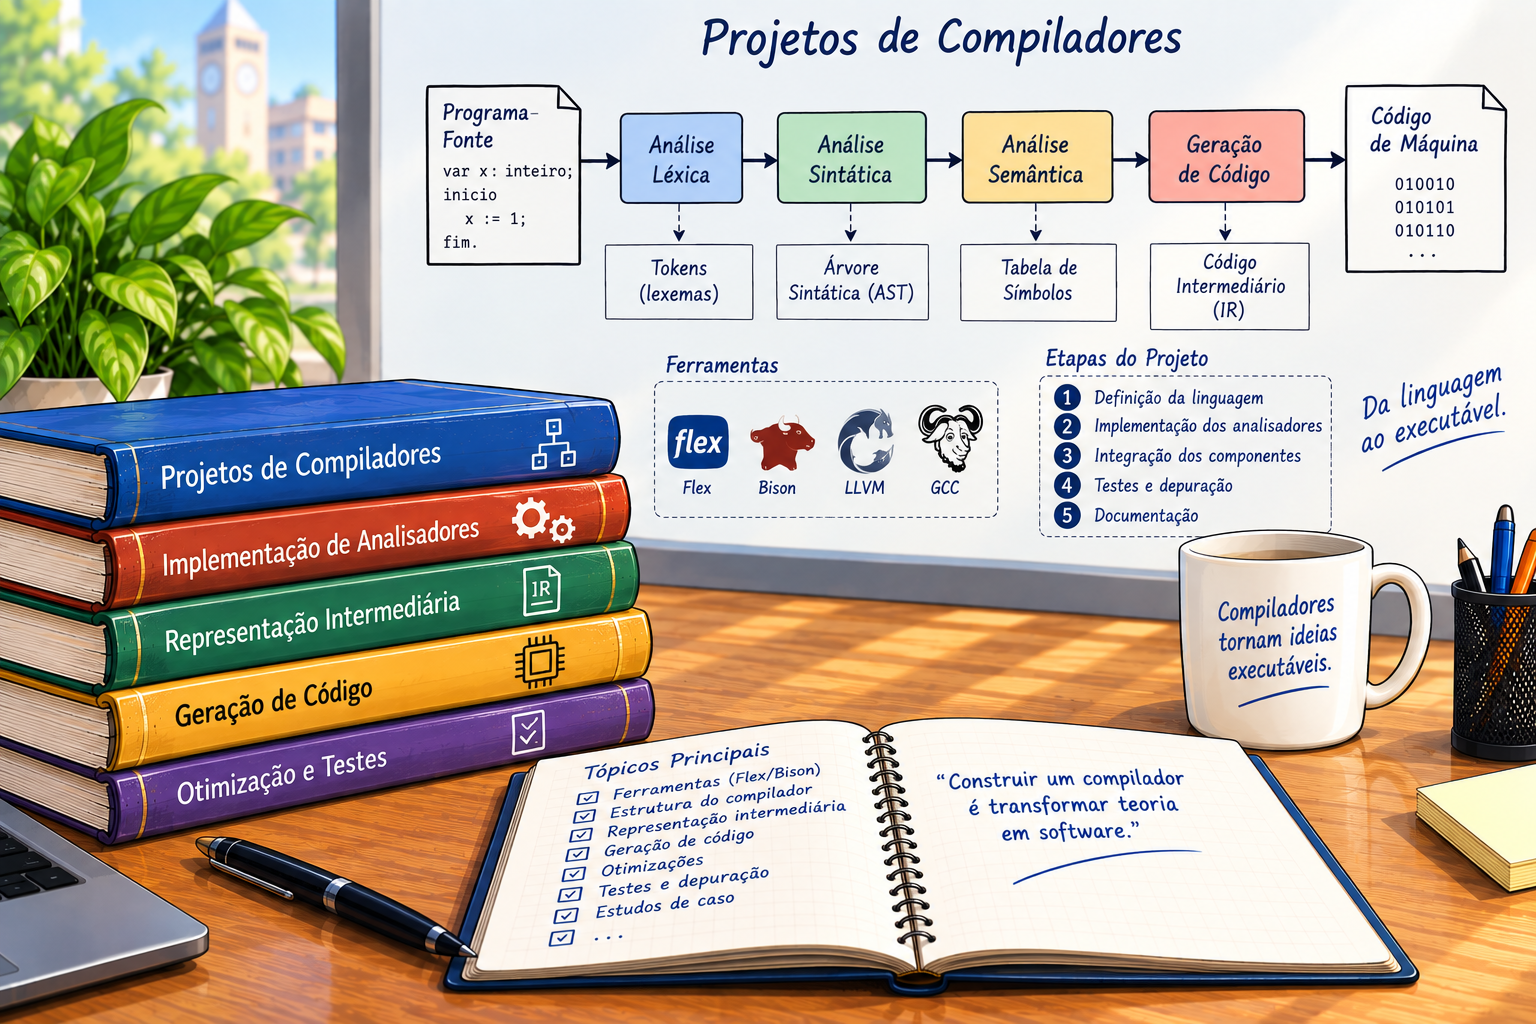
\includegraphics[width=0.7\linewidth,height=\textheight,keepaspectratio]{chapters/images/projetos.png}
\end{center}

A seguir está uma versão desenvolvida para o livro Teoria de Linguagens
e Compiladores, mantendo a organização conceitual dos slides e
aprofundando as explicações sobre a relação entre compilador, memória,
pilha de execução, árvore de ativação e registros de ativação. O texto
também estabelece a ligação com o projeto de compilador para a MVS,
especialmente com a implementação de funções, procedimentos e passagem
de parâmetros.

\section{Ambientes de execução}\label{ambientes-de-execuuxe7uxe3o}

A geração de código não encerra o processo de implementação de uma
linguagem de programação. Para que um programa compilado possa ser
executado corretamente, é necessário estabelecer como suas instruções e
seus dados serão organizados na memória e como ocorrerão as chamadas de
funções e procedimentos.

Essas decisões envolvem um compromisso entre o compilador, o sistema
operacional, a arquitetura da máquina de destino e, quando existente, o
ambiente de execução da linguagem. O compilador precisa produzir código
que respeite as convenções adotadas por esses componentes, de modo que
as instruções geradas possam ser executadas corretamente.

Para isso, considera-se um modelo denominado ambiente de execução
(runtime environment). Esse modelo define as estruturas e os mecanismos
utilizados durante a execução do programa, incluindo:

\begin{itemize}
\tightlist
\item
  a localização e a alocação do código e dos dados;
\item
  o acesso a variáveis globais, locais e parâmetros;
\item
  o gerenciamento da memória utilizada pelas funções e pelos
  procedimentos;
\item
  os mecanismos de chamada e retorno de rotinas;
\item
  as convenções de passagem de parâmetros e de retorno de valores;
\item
  a comunicação com o sistema operacional, incluindo operações de
  entrada e saída.
\end{itemize}

O ambiente de execução estabelece, portanto, as condições necessárias
para que as abstrações da linguagem de programação sejam implementadas
sobre uma máquina concreta ou virtual.

Considere uma função que recebe dois parâmetros, realiza uma operação
aritmética e retorna o resultado. Para executá-la, não basta que o
compilador gere a instrução de adição. Também é necessário determinar
onde os parâmetros serão armazenados, como as variáveis locais serão
acessadas, onde o resultado será colocado e como o controle retornará ao
ponto da chamada.

Essas decisões fazem parte da organização do ambiente de execução. Uma
vez estabelecidas, o compilador pode traduzir funções e procedimentos
utilizando uma convenção consistente de armazenamento de dados, chamada
e retorno.

No caso de uma máquina virtual didática, como a MVS utilizada neste
livro, esse ambiente pode ser simplificado para fins pedagógicos. Ainda
assim, os mesmos princípios precisam ser considerados quando a linguagem
passa a oferecer subprogramas, parâmetros e chamadas recursivas.

\subsection{Organização da
memória}\label{organizauxe7uxe3o-da-memuxf3ria}

Durante a execução, um programa utiliza diferentes regiões de memória,
cada uma destinada a finalidades específicas. Uma organização conceitual
comum distingue a área de código, a área de dados globais ou estáticos,
a pilha de execução e a área de alocação dinâmica, denominada heap.

\begin{figure}

\centering{

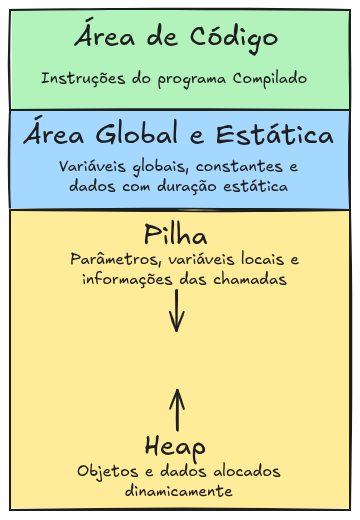
\includegraphics[width=0.3\linewidth,height=\textheight,keepaspectratio]{chapters/images/organizacao-memoria.png}

}

\caption{\label{fig-organizacao}Representação conceitual das regiões de
memória}

\end{figure}%

Uma representação conceitual das regiões de memória está ilustrada na
Figura~\ref{fig-organizacao}. A disposição física e o sentido de
crescimento das regiões dependem da plataforma.

A área de código contém as instruções executáveis do programa. Seu
conteúdo é produzido pelo compilador ou pelo sistema de ligação e,
normalmente, permanece estável durante a execução. Em programas
convencionais, o tamanho do código pode ser determinado a partir do
executável produzido, embora existam mecanismos que permitem carregar
código adicional durante a execução.

A área global ou estática armazena dados cuja duração não depende de uma
chamada individual de função. Entre os exemplos estão variáveis globais
e variáveis estáticas. O espaço necessário para esses dados pode ser
determinado durante a compilação ou a ligação do programa.

A pilha de execução armazena informações relacionadas às chamadas de
funções e procedimentos. Cada chamada pode exigir espaço para os
parâmetros, as variáveis locais, os valores temporários e o endereço de
retorno. Esse espaço é organizado em registros de ativação, que serão
estudados adiante.

A heap é utilizada para dados cuja alocação e duração são controladas
durante a execução. Por exemplo, um programa pode solicitar memória
dinamicamente para armazenar uma estrutura de dados cujo tamanho só é
conhecido em tempo de execução. A liberação desse espaço pode ser
explícita, como em \texttt{free} e \texttt{delete}, ou automática, por
meio de mecanismos de gerenciamento e coleta de lixo.

É importante distinguir a heap da pilha de execução. A pilha organiza
principalmente as informações associadas às chamadas de rotinas,
enquanto a heap permite manter objetos e estruturas de dados que
precisam existir independentemente do término de uma chamada específica.

Essa divisão é conceitual: sistemas operacionais e arquiteturas reais
podem utilizar outras regiões, como áreas de memória mapeadas,
bibliotecas compartilhadas e pilhas específicas para diferentes threads.

\subsection{Memória estática e
dinâmica}\label{memuxf3ria-estuxe1tica-e-dinuxe2mica}

A localização dos dados e sua duração são aspectos fundamentais para o
gerenciamento da memória.

A alocação estática ocorre quando o espaço necessário para determinados
dados é estabelecido antes da execução, geralmente durante a compilação
ou a ligação. Variáveis globais e variáveis estáticas são exemplos
comuns. Como sua localização é conhecida pelo ambiente de execução, o
acesso a esses dados pode ser realizado por endereços previamente
determinados.

A alocação dinâmica ocorre durante a execução. O espaço necessário é
obtido conforme as operações realizadas pelo programa. A pilha de
execução é utilizada para gerenciar as ativações de funções e
procedimentos, enquanto a heap é utilizada para objetos e estruturas
cuja duração não precisa acompanhar a sequência de chamadas.

Considere o seguinte programa:

\begin{Shaded}
\begin{Highlighting}[]
\DataTypeTok{int}\NormalTok{ total}\OperatorTok{;}

\DataTypeTok{void}\NormalTok{ calcula}\OperatorTok{(}\DataTypeTok{int}\NormalTok{ n}\OperatorTok{)} \OperatorTok{\{}
    \DataTypeTok{int}\NormalTok{ parcial}\OperatorTok{;}
\NormalTok{    parcial }\OperatorTok{=}\NormalTok{ n }\OperatorTok{*} \DecValTok{2}\OperatorTok{;}
\OperatorTok{\}}
\end{Highlighting}
\end{Shaded}

A variável global \texttt{total} possui duração estática. Já o parâmetro
\texttt{n} e a variável local \texttt{parcial} estão associados à
execução de \texttt{calcula}. Em uma implementação que utiliza pilha de
execução, o espaço para esses dados pode ser reservado em um registro de
ativação criado quando a função é chamada e liberado quando ela retorna.

Se a função for chamada várias vezes, cada ativação poderá possuir seus
próprios valores para \texttt{n} e \texttt{parcial}. Essa característica
é indispensável para que chamadas sucessivas ou recursivas não
compartilhem indevidamente as variáveis locais.

A distinção entre alocação estática e dinâmica não deve ser confundida
com a distinção entre pilha e heap. A primeira diz respeito ao momento e
à duração da alocação; a segunda identifica regiões e mecanismos de
gerenciamento de memória. A pilha, por exemplo, realiza alocação
dinâmica em tempo de execução, mesmo que o tamanho de cada registro de
ativação possa ser calculado pelo compilador.

\section{Pilha de execução}\label{pilha-de-execuuxe7uxe3o}

A pilha de execução é uma estrutura de dados utilizada para gerenciar as
chamadas e os retornos das funções e dos procedimentos. Sua organização
segue a disciplina LIFO (Last In, First Out): o último elemento inserido
é o primeiro a ser removido.

Quando uma rotina é chamada, o ambiente de execução reserva espaço para
as informações necessárias à sua execução. Esse espaço constitui seu
registro de ativação. Quando a rotina termina, o registro correspondente
é removido, liberando o espaço utilizado e permitindo que a execução
continue no ponto de chamada.

Considere o seguinte programa:

\begin{Shaded}
\begin{Highlighting}[]
\DataTypeTok{void}\NormalTok{ C}\OperatorTok{()} \OperatorTok{\{}
    \CommentTok{/* comandos de C */}
\OperatorTok{\}}

\DataTypeTok{void}\NormalTok{ B}\OperatorTok{()} \OperatorTok{\{}
\NormalTok{    C}\OperatorTok{();}
\OperatorTok{\}}

\DataTypeTok{int}\NormalTok{ main}\OperatorTok{()} \OperatorTok{\{}
\NormalTok{    B}\OperatorTok{();}
    \ControlFlowTok{return} \DecValTok{0}\OperatorTok{;}
\OperatorTok{\}}
\end{Highlighting}
\end{Shaded}

A execução começa em \texttt{main}, que chama \texttt{B}. Durante a
execução de \texttt{B}, ocorre uma chamada a \texttt{C}. Nesse momento,
as três rotinas possuem ativações vivas: \texttt{main}, \texttt{B} e
\texttt{C}.

\begin{figure}

\centering{

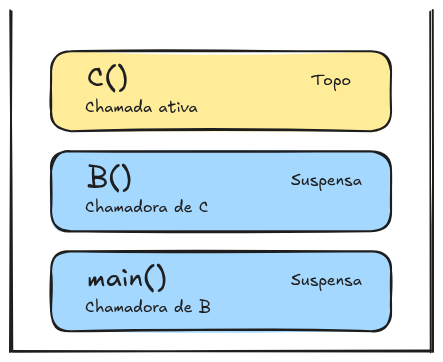
\includegraphics[width=0.3\linewidth,height=\textheight,keepaspectratio]{chapters/images/pilha-ativacao.png}

}

\caption{\label{fig-pilha-ativacao}Estado da pilha durante a execução de
C}

\end{figure}%

A representação na Figura~\ref{fig-pilha-ativacao} mostra a ordem lógica
dos registros, do topo para a base. A disposição física da memória pode
variar.

Quando \texttt{C} termina, seu registro de ativação é removido e o
controle retorna a \texttt{B}. Depois que \texttt{B} termina, seu
registro é removido, e a execução retorna a \texttt{main}. Por fim, a
ativação de \texttt{main} termina.

A pilha permite que o ambiente de execução preserve o contexto de cada
chamada sem precisar reservar antecipadamente um espaço exclusivo para
todas as chamadas possíveis de uma rotina. O mesmo código de uma função
pode ser executado repetidas vezes, utilizando registros de ativação
diferentes.

Essa organização é especialmente importante na recursão. Uma função
recursiva chama a si própria, direta ou indiretamente, antes que uma
ativação anterior tenha terminado. Cada chamada precisa preservar seus
parâmetros, suas variáveis locais e seu endereço de retorno. A pilha
oferece um mecanismo natural para organizar essas informações.

\subsection{Por que a pilha funciona?}\label{por-que-a-pilha-funciona}

O uso de uma pilha de execução é possível porque as chamadas de funções
e procedimentos apresentam uma propriedade de aninhamento. Uma rotina
chamada durante a execução de outra precisa terminar antes que a
execução da rotina chamadora possa continuar após a chamada, no modelo
convencional de chamadas síncronas.

Isso significa que a ordem das ativações e dos retornos é compatível com
a disciplina LIFO:

\begin{itemize}
\tightlist
\item
  as ativações são iniciadas na ordem em que as chamadas ocorrem;
\item
  a ativação mais recente precisa terminar antes que a ativação
  imediatamente anterior possa continuar após a chamada;
\item
  os registros são removidos na ordem inversa àquela em que foram
  criados.
\end{itemize}

Essa propriedade explica por que não é necessário procurar
arbitrariamente qual ativação deve ser encerrada: em uma execução
convencional, o registro no topo da pilha corresponde à rotina
atualmente ativa.

A afirmação pressupõe chamadas síncronas convencionais. Corrotinas,
continuations, execução assíncrona e outros mecanismos podem exigir
estruturas de controle adicionais ou gerenciamento de contexto
diferente.

\section{Árvore de ativação}\label{uxe1rvore-de-ativauxe7uxe3o}

A árvore de ativação é uma representação conceitual da sequência de
chamadas de funções e procedimentos durante a execução de um programa.
Ela permite visualizar a relação entre uma ativação e as ativações que
ocorrem durante sua execução.

Cada nó da árvore representa uma ativação específica de uma rotina. Se,
durante a ativação de uma rotina \(A\), ocorre uma chamada que cria a
ativação \(B\), então \(B\) é representada como filha de \(A\).

É importante observar que os nós representam chamadas, e não apenas
nomes de funções. Se uma função recursiva for chamada várias vezes, cada
chamada será representada por um nó distinto, mesmo que todos os nós
correspondam ao mesmo código-fonte.

\subsection{Exemplo: ordenação por
quicksort}\label{exemplo-ordenauxe7uxe3o-por-quicksort}

Considere o seguinte programa simplificado, que utiliza o algoritmo de
ordenação quicksort:

\begin{Shaded}
\begin{Highlighting}[]
\PreprocessorTok{\#include }\ImportTok{\textless{}stdio.h\textgreater{}}
\PreprocessorTok{\#include }\ImportTok{\textless{}stdlib.h\textgreater{}}
\PreprocessorTok{\#include }\ImportTok{\textless{}string.h\textgreater{}}

\PreprocessorTok{\#define DEBUG}\OperatorTok{(}\PreprocessorTok{x}\OperatorTok{)}\PreprocessorTok{ x}
\PreprocessorTok{\#define TAM }\DecValTok{10}
\DataTypeTok{int}\NormalTok{ a}\OperatorTok{[}\NormalTok{TAM }\OperatorTok{+} \DecValTok{1}\OperatorTok{]} \OperatorTok{=} 
  \OperatorTok{\{}\DecValTok{95}\OperatorTok{,} \DecValTok{60}\OperatorTok{,} \DecValTok{10}\OperatorTok{,} \DecValTok{40}\OperatorTok{,} \DecValTok{30}\OperatorTok{,} \DecValTok{1}\OperatorTok{,} \DecValTok{20}\OperatorTok{,} \DecValTok{90}\OperatorTok{,} \DecValTok{70}\OperatorTok{,} \DecValTok{80}\OperatorTok{,} \DecValTok{50}\OperatorTok{\};}

\DataTypeTok{int}\NormalTok{ partition}\OperatorTok{(}\DataTypeTok{int}\NormalTok{ p}\OperatorTok{,} \DataTypeTok{int}\NormalTok{ r}\OperatorTok{)}
\OperatorTok{\{}
    \DataTypeTok{int}\NormalTok{ x }\OperatorTok{=}\NormalTok{ a}\OperatorTok{[}\NormalTok{r}\OperatorTok{];} \CommentTok{/* pivo */}
    \DataTypeTok{int}\NormalTok{ i }\OperatorTok{=}\NormalTok{ p }\OperatorTok{{-}} \DecValTok{1}\OperatorTok{;}
    \DataTypeTok{int}\NormalTok{ j}\OperatorTok{,}\NormalTok{ temp}\OperatorTok{;}
    \ControlFlowTok{for} \OperatorTok{(}\NormalTok{j }\OperatorTok{=}\NormalTok{ p}\OperatorTok{;}\NormalTok{ j }\OperatorTok{\textless{}}\NormalTok{ r}\OperatorTok{;}\NormalTok{ j}\OperatorTok{++)}
    \OperatorTok{\{}
        \ControlFlowTok{if} \OperatorTok{(}\NormalTok{a}\OperatorTok{[}\NormalTok{j}\OperatorTok{]} \OperatorTok{\textless{}=}\NormalTok{ x}\OperatorTok{)}
        \OperatorTok{\{}
\NormalTok{            i}\OperatorTok{++;}
\NormalTok{            temp }\OperatorTok{=}\NormalTok{ a}\OperatorTok{[}\NormalTok{i}\OperatorTok{];}
\NormalTok{            a}\OperatorTok{[}\NormalTok{i}\OperatorTok{]} \OperatorTok{=}\NormalTok{ a}\OperatorTok{[}\NormalTok{j}\OperatorTok{];}
\NormalTok{            a}\OperatorTok{[}\NormalTok{j}\OperatorTok{]} \OperatorTok{=}\NormalTok{ temp}\OperatorTok{;}
        \OperatorTok{\}}
    \OperatorTok{\}}
\NormalTok{    temp }\OperatorTok{=}\NormalTok{ a}\OperatorTok{[}\NormalTok{i }\OperatorTok{+} \DecValTok{1}\OperatorTok{];}
\NormalTok{    a}\OperatorTok{[}\NormalTok{i }\OperatorTok{+} \DecValTok{1}\OperatorTok{]} \OperatorTok{=}\NormalTok{ a}\OperatorTok{[}\NormalTok{r}\OperatorTok{];}
\NormalTok{    a}\OperatorTok{[}\NormalTok{r}\OperatorTok{]} \OperatorTok{=}\NormalTok{ temp}\OperatorTok{;}
    \ControlFlowTok{return}\NormalTok{ i }\OperatorTok{+} \DecValTok{1}\OperatorTok{;}
\OperatorTok{\}}

\DataTypeTok{void}\NormalTok{ qSort}\OperatorTok{(}\DataTypeTok{int}\NormalTok{ m}\OperatorTok{,} \DataTypeTok{int}\NormalTok{ n}\OperatorTok{,} \DataTypeTok{int}\NormalTok{ level}\OperatorTok{)}
\OperatorTok{\{}
    \DataTypeTok{char}\NormalTok{ tab}\OperatorTok{[}\DecValTok{40}\OperatorTok{]} \OperatorTok{=} \StringTok{""}\OperatorTok{;}
    \ControlFlowTok{for} \OperatorTok{(}\DataTypeTok{int}\NormalTok{ i }\OperatorTok{=} \DecValTok{0}\OperatorTok{;}\NormalTok{ i }\OperatorTok{\textless{}}\NormalTok{ level}\OperatorTok{;}\NormalTok{ i}\OperatorTok{++)}
\NormalTok{       strcat}\OperatorTok{(}\NormalTok{tab}\OperatorTok{,}\StringTok{"..."}\OperatorTok{);}
\NormalTok{    DEBUG}\OperatorTok{(}\NormalTok{printf}\OperatorTok{(}\StringTok{"}\SpecialCharTok{\%s}\StringTok{Entra no qSort(}\SpecialCharTok{\%d}\StringTok{,}\SpecialCharTok{\%d}\StringTok{)}\SpecialCharTok{\textbackslash{}n}\StringTok{"}\OperatorTok{,}\NormalTok{ tab}\OperatorTok{,}\NormalTok{ m}\OperatorTok{,}\NormalTok{ n}\OperatorTok{);)}
    \ControlFlowTok{if} \OperatorTok{(}\NormalTok{m }\OperatorTok{\textless{}}\NormalTok{ n}\OperatorTok{)}
    \OperatorTok{\{}
        \DataTypeTok{int}\NormalTok{ i }\OperatorTok{=}\NormalTok{ partition}\OperatorTok{(}\NormalTok{m}\OperatorTok{,}\NormalTok{ n}\OperatorTok{);}
\NormalTok{        qSort}\OperatorTok{(}\NormalTok{m}\OperatorTok{,}\NormalTok{ i }\OperatorTok{{-}} \DecValTok{1}\OperatorTok{,}\NormalTok{ level}\OperatorTok{+}\DecValTok{1}\OperatorTok{);}
\NormalTok{        qSort}\OperatorTok{(}\NormalTok{i }\OperatorTok{+} \DecValTok{1}\OperatorTok{,}\NormalTok{ n}\OperatorTok{,}\NormalTok{ level}\OperatorTok{+}\DecValTok{1}\OperatorTok{);}
    \OperatorTok{\}}
\NormalTok{    DEBUG}\OperatorTok{(}\NormalTok{printf}\OperatorTok{(}\StringTok{"}\SpecialCharTok{\%s}\StringTok{Sai do qSort(}\SpecialCharTok{\%d}\StringTok{,}\SpecialCharTok{\%d}\StringTok{)}\SpecialCharTok{\textbackslash{}n}\StringTok{"}\OperatorTok{,}\NormalTok{ tab}\OperatorTok{,}\NormalTok{ m}\OperatorTok{,}\NormalTok{ n}\OperatorTok{);)}
\OperatorTok{\}}

\DataTypeTok{int}\NormalTok{ main}\OperatorTok{()}
\OperatorTok{\{}
\NormalTok{    DEBUG}\OperatorTok{(}\NormalTok{printf}\OperatorTok{(}\StringTok{"Entra no main()}\SpecialCharTok{\textbackslash{}n}\StringTok{"}\OperatorTok{);)}
\NormalTok{    qSort}\OperatorTok{(}\DecValTok{0}\OperatorTok{,}\NormalTok{ TAM}\OperatorTok{,} \DecValTok{1}\OperatorTok{);}
    \ControlFlowTok{for} \OperatorTok{(}\DataTypeTok{int}\NormalTok{ i }\OperatorTok{=} \DecValTok{0}\OperatorTok{;}\NormalTok{ i }\OperatorTok{\textless{}}\NormalTok{ TAM}\OperatorTok{+}\DecValTok{1}\OperatorTok{;}\NormalTok{ i}\OperatorTok{++)}
\NormalTok{      printf}\OperatorTok{(}\StringTok{"}\SpecialCharTok{\%4d}\StringTok{"}\OperatorTok{,}\NormalTok{ a}\OperatorTok{[}\NormalTok{i}\OperatorTok{]);}
\NormalTok{    puts}\OperatorTok{(}\StringTok{""}\OperatorTok{);}
\NormalTok{    DEBUG}\OperatorTok{(}\NormalTok{printf}\OperatorTok{(}\StringTok{"Sai do main()}\SpecialCharTok{\textbackslash{}n}\StringTok{"}\OperatorTok{);)}
    \ControlFlowTok{return} \OperatorTok{(}\NormalTok{EXIT\_SUCCESS}\OperatorTok{);}
\OperatorTok{\}}
\end{Highlighting}
\end{Shaded}

O programa principal chama \texttt{qSort}. Durante a execução de
\texttt{qSort}, ocorre uma chamada a \texttt{partition} e,
posteriormente, duas chamadas recursivas a \texttt{qSort}.

Uma possível sequência simplificada de execução, sem as chamadas a
\texttt{partition} é:

\begin{verbatim}
Entra no main()
...Entra no qSort(0,10)
......Entra no qSort(0,4)
.........Entra no qSort(0,1)
............Entra no qSort(0,-1)
............Sai do qSort(0,-1)
............Entra no qSort(1,1)
............Sai do qSort(1,1)
.........Sai do qSort(0,1)
.........Entra no qSort(3,4)
............Entra no qSort(3,2)
............Sai do qSort(3,2)
............Entra no qSort(4,4)
............Sai do qSort(4,4)
.........Sai do qSort(3,4)
......Sai do qSort(0,4)
......Entra no qSort(6,10)
.........Entra no qSort(6,5)
.........Sai do qSort(6,5)
.........Entra no qSort(7,10)
............Entra no qSort(7,9)
...............Entra no qSort(7,7)
...............Sai do qSort(7,7)
...............Entra no qSort(9,9)
...............Sai do qSort(9,9)
............Sai do qSort(7,9)
............Entra no qSort(11,10)
............Sai do qSort(11,10)
.........Sai do qSort(7,10)
......Sai do qSort(6,10)
...Sai do qSort(0,10)
   1  10  20  30  40  50  60  70  80  90  95
Sai do main()
\end{verbatim}

A árvore de ativação correspondente pode ser representada da seguinte
maneira:

\begin{figure}

\centering{

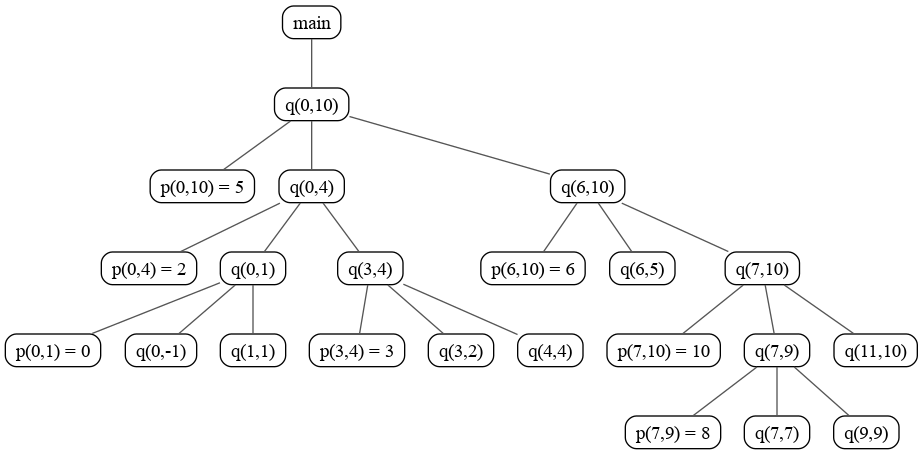
\includegraphics[width=0.8\linewidth,height=\textheight,keepaspectratio]{chapters/images/qsort1.png}

}

\caption{\label{fig-qsort1}Árvore de ativação completa}

\end{figure}%

Na árvore de ativação da Figura~\ref{fig-qsort1} cada nó representa uma
chamada específica, e os filhos são as ativações iniciadas durante a
execução do nó pai.

Na árvore completa, as chamadas recursivas de \texttt{qSort} também
podem originar outras chamadas a \texttt{partition} e novas ativações de
\texttt{qSort}, até que os subvetores tenham tamanho suficiente para
encerrar a recursão.

A árvore de ativação permite distinguir duas representações importantes:
a árvore descreve todas as relações de chamada ocorridas durante a
execução considerada, enquanto a pilha representa apenas as ativações
que permanecem vivas em um determinado instante.

\subsection{Relação entre a árvore de ativação e a
pilha}\label{relauxe7uxe3o-entre-a-uxe1rvore-de-ativauxe7uxe3o-e-a-pilha}

A sequência de chamadas de um programa corresponde a um percurso em
pré-ordem na árvore de ativação, considerando que cada nó é visitado
quando sua ativação começa e que as chamadas filhas são visitadas na
ordem em que ocorrem.

De maneira análoga, a sequência de retornos corresponde a um percurso em
pós-ordem, considerando que um nó termina depois de concluídas as
ativações filhas.

Em qualquer instante, as ativações vivas formam o caminho entre a raiz
da árvore e o nó correspondente à rotina que está em execução. A pilha
contém os registros dessas ativações, com o registro da rotina atual no
topo.

A Figura~\ref{fig-qsort2} apresenta as ativações já finalizadas (na cor
verde), as ativações suspensas na pilha de execução (na cor azul), para
a chamada ativa \texttt{qSort(3,2)}. As ativações que ainda não foram
realizadas até este instantes estão representadas com linhas
pontilhadas.

\begin{figure}

\centering{

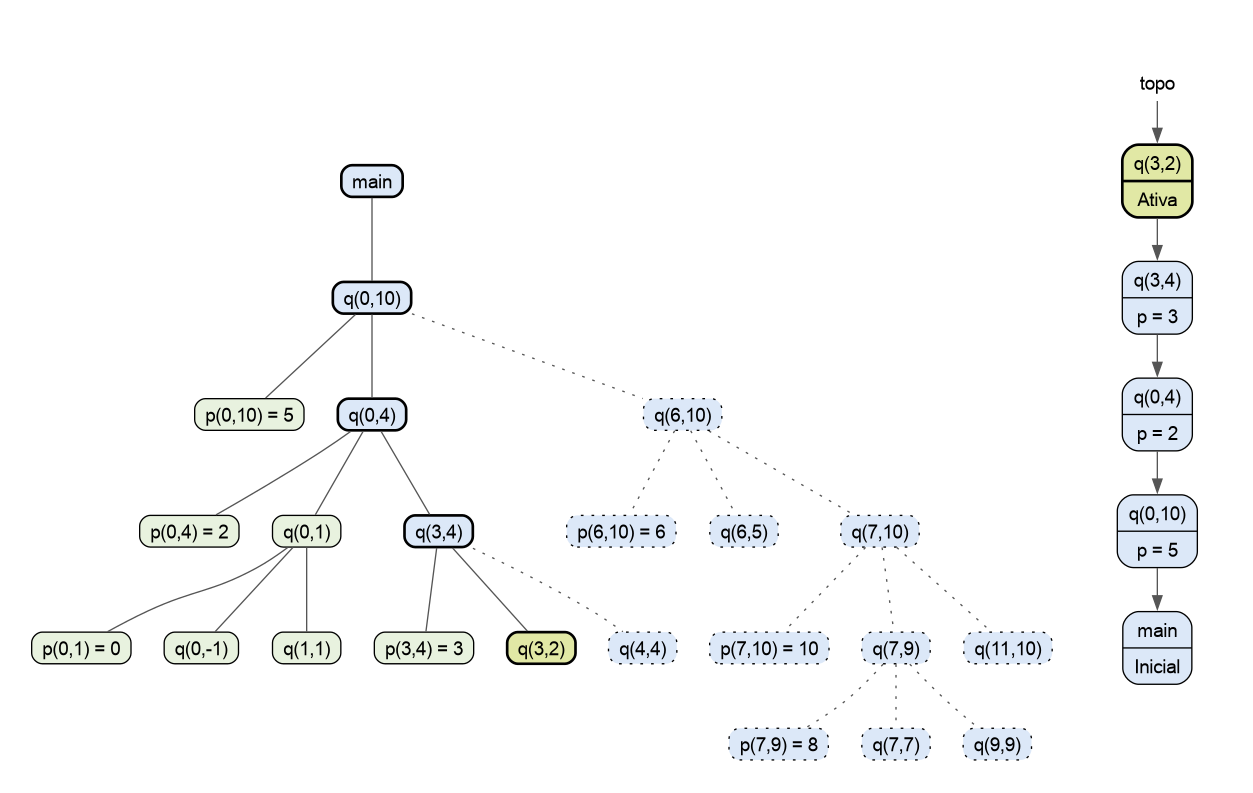
\includegraphics[width=0.9\linewidth,height=\textheight,keepaspectratio]{chapters/images/qsort2.png}

}

\caption{\label{fig-qsort2}Árvore de ativação até a chamada
\texttt{qSort(3,2)} e a pilha de ativação correspondente}

\end{figure}%

A pilha contém os registros correspondentes a cinco ativações até a
chamada \texttt{qSort(3,2)}. Quando \texttt{partition(3,4)} termina, seu
registro é removido, e a execução retorna a \texttt{qSort(3,4)} que
então inicia a primeira chamada \texttt{qSort(3,2)}. A pilha de ativação
passa então a conter as chamadas \texttt{qSort(3,2)},
\texttt{qSort(3,4)}, \texttt{qSort(0,4)}, \texttt{qSort(0,10)} e
\texttt{main}.

A árvore de ativação oferece, portanto, uma visão global da estrutura de
chamadas, enquanto a pilha de execução representa o estado ativo dessa
estrutura em um momento específico. Essa relação é fundamental para
compreender o gerenciamento de funções, procedimentos e recursão.

A simulação seguinte ilustra o processo de acompanhamento das chamadas
recursivas:

\begin{figure}[H]
\centering
\fbox{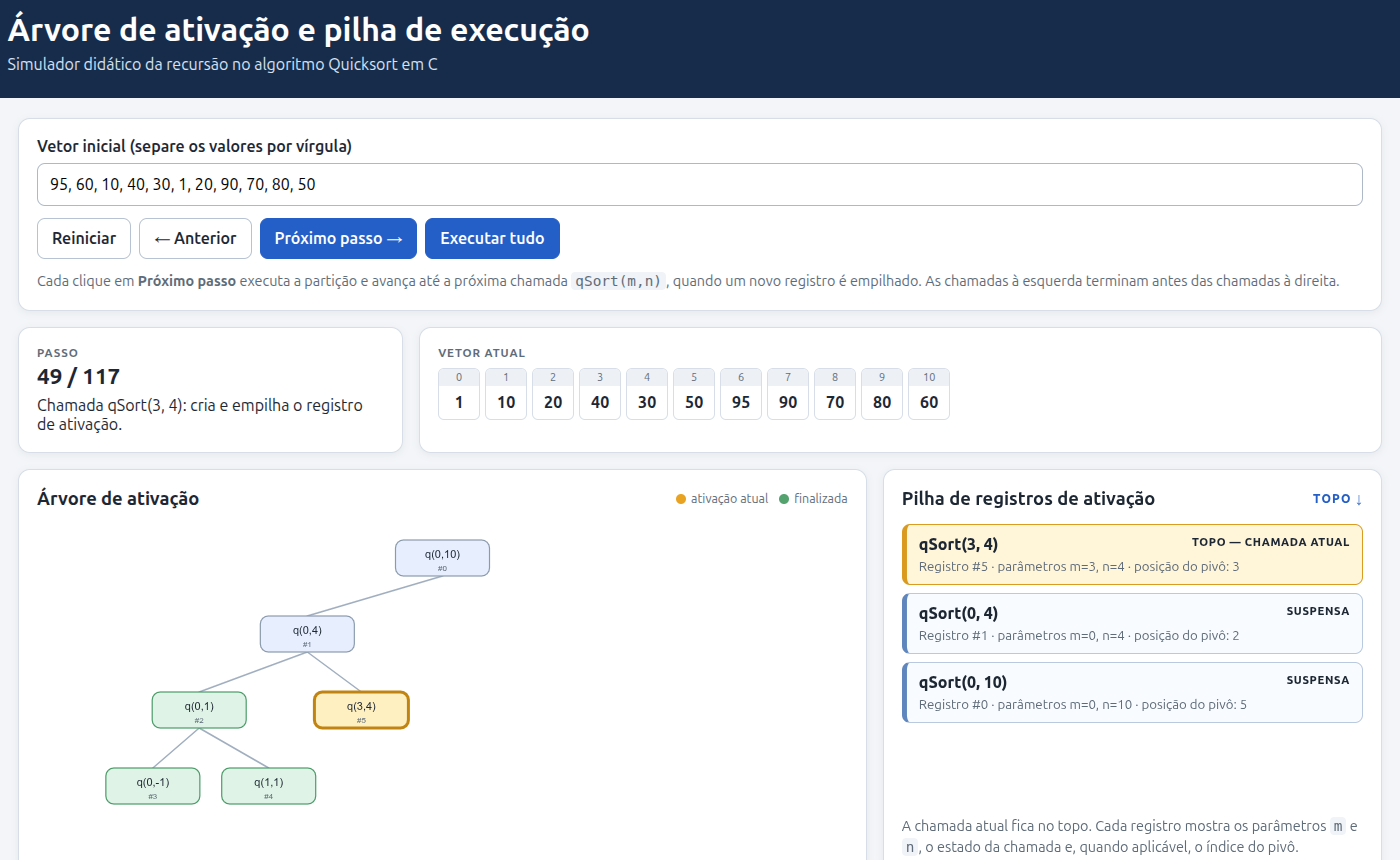
\includegraphics[width=0.6\textwidth]{chapters/images/printscreen/ativTree.png}}
\caption{Visualização da aplicação interativa}
\end{figure}
\begin{tcolorbox}[enhanced jigsaw, title=Acesso Interativo]
Acesse a simulação em:\par\smallskip
\small\url{https://luizedsilva.github.io/Livro-LTC/p5js/ativTree/}
\begin{center}
\includegraphics[width=3cm]{chapters/images/qrcode/ativTree.png}\end{center}
\end{tcolorbox}

\section{Registro de ativação}\label{registro-de-ativauxe7uxe3o}

Quando uma função ou procedimento é chamado, o ambiente de execução
precisa preservar as informações necessárias para que a rotina seja
executada corretamente e, ao terminar, retorne ao ponto de chamada. O
conjunto dessas informações constitui o registro de ativação, também
denominado frame.

Cada ativação possui seu próprio registro. Assim, duas chamadas da mesma
função podem compartilhar o código executável, mas manter parâmetros,
variáveis locais e endereços de retorno diferentes.

Um registro de ativação pode conter as seguintes informações:

\begin{itemize}
\tightlist
\item
  Parâmetros: valores ou referências recebidos na chamada.
\item
  Variáveis locais: dados declarados no corpo da rotina.
\item
  Valores temporários: resultados intermediários utilizados na avaliação
  de expressões.
\item
  Estado da máquina: informações que precisam ser preservadas durante a
  chamada, como registradores utilizados pelo chamador.
\item
  Endereço de retorno: endereço da instrução que deverá ser executada
  depois que a rotina terminar.
\item
  Elo de controle: referência ao registro de ativação da rotina
  chamadora.
\item
  Elo de acesso: referência utilizada para localizar dados de escopos
  lexicais externos, quando a linguagem e sua implementação exigem esse
  mecanismo.
\item
  Espaço para o resultado: local utilizado para devolver o valor de uma
  função, conforme a convenção de chamada.
\end{itemize}

Nem todos os registros de ativação contêm necessariamente todos esses
campos. A organização depende da linguagem, da arquitetura e da
convenção de chamada. Por exemplo, alguns parâmetros podem ser
transmitidos por registradores, e o valor retornado pode ser colocado em
um registrador específico, em vez de ocupar uma posição no registro de
ativação.

\subsection{Organização de um registro de
ativação}\label{organizauxe7uxe3o-de-um-registro-de-ativauxe7uxe3o}

A Figura~\ref{fig-registro-conceitual} apresenta uma organização
conceitual possível.

\begin{figure}

\centering{

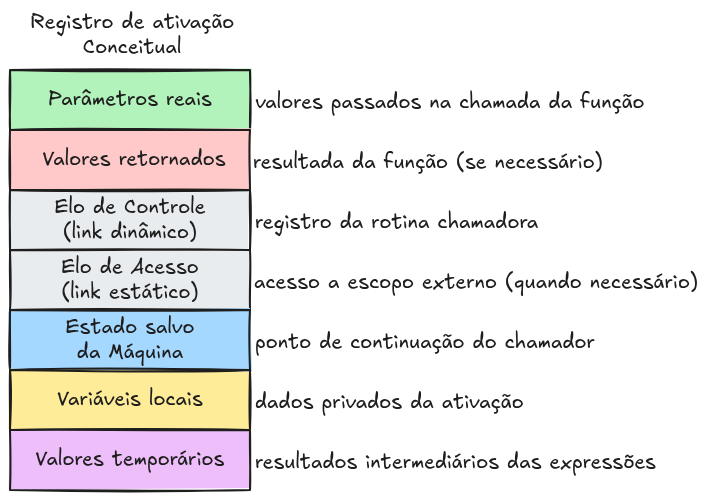
\includegraphics[width=0.6\linewidth,height=\textheight,keepaspectratio]{chapters/images/registro-ativacao-conceitual.png}

}

\caption{\label{fig-registro-conceitual}Registro de ativação conceitual}

\end{figure}%

Os campos são ilustrativos. Sua ordem, presença e forma de armazenamento
variam conforme a implementação.

O registro é criado quando uma ativação começa e permanece disponível
enquanto a rotina está em execução. Quando a rotina termina, o ambiente
de execução utiliza as informações necessárias para restaurar o contexto
do chamador e liberar o espaço correspondente.

Essa organização permite que o compilador utilize deslocamentos
relativos para acessar os dados locais. Por exemplo, uma variável pode
ser localizada a partir de um registrador que aponta para uma posição de
referência do registro de ativação. O deslocamento da variável pode
permanecer constante em diferentes chamadas, mesmo que cada registro
esteja localizado em uma posição diferente da memória.

\subsection{Elo de controle e elo de
acesso}\label{elo-de-controle-e-elo-de-acesso}

Embora possam ser representados por referências entre registros, o elo
de controle e o elo de acesso têm finalidades distintas.

O elo de controle identifica a relação dinâmica entre a rotina chamada e
a rotina que a chamou. Ele permite recuperar o contexto anterior quando
a execução retorna. Em uma implementação baseada em pilha, essa relação
acompanha a sequência efetiva de chamadas.

O elo de acesso permite localizar dados pertencentes a um escopo lexical
externo. Ele é relevante em linguagens que permitem declarar rotinas
dentro de outras rotinas e acessar variáveis de escopos envolventes. Sua
utilização depende das regras de escopo da linguagem e da estratégia de
implementação.

Em programas nos quais todas as rotinas são declaradas em um único nível
e não existe acesso a variáveis de escopos externos, o elo de acesso
pode ser desnecessário.

Essa distinção é importante porque a relação entre rotinas na estrutura
lexical do programa não é necessariamente a mesma relação estabelecida
pela sequência de chamadas durante a execução.

\section{Relação com o projeto de compilador para a
MVS}\label{relauxe7uxe3o-com-o-projeto-de-compilador-para-a-mvs}

Os conceitos apresentados fornecem a base para ampliar o compilador
desenvolvido nos capítulos anteriores, permitindo a implementação de
funções, procedimentos, passagem de parâmetros e recursão.

No projeto atual, a tabela de símbolos armazena informações sobre os
identificadores, incluindo seu nome, endereço e tipo. Para incorporar
subprogramas, será necessário acrescentar informações sobre parâmetros
formais, tipo de retorno e localização do código correspondente. Também
será preciso estabelecer como os parâmetros e as variáveis locais serão
armazenados durante cada ativação.

A implementação pode seguir uma sequência incremental:

\begin{enumerate}
\def\labelenumi{\arabic{enumi}.}
\tightlist
\item
  Definir a convenção de chamada e retorno da MVS.
\item
  Implementar chamadas de procedimentos sem parâmetros.
\item
  Introduzir parâmetros por valor e verificar quantidade e tipos dos
  argumentos.
\item
  Implementar o retorno de valores das funções.
\item
  Organizar variáveis locais e registros de ativação para permitir
  chamadas recursivas.
\item
  Incorporar passagem por referência e, se necessário, mecanismos de
  acesso a escopos externos.
\end{enumerate}

A MVS precisará oferecer instruções ou mecanismos equivalentes para
preservar o endereço de retorno, transferir o controle para o
subprograma e restaurar a execução do chamador. Se o conjunto de
instruções atual não oferecer esses recursos, será necessário ampliá-lo
ou implementar uma convenção de chamada usando as instruções existentes.

A pilha de execução, a árvore de ativação e o registro de ativação
descrevem aspectos complementares desse processo. A árvore representa a
relação entre as chamadas; a pilha mantém as ativações vivas; e cada
registro reúne os dados e o contexto necessários à execução de uma
rotina.

Esses conceitos completam o estudo da geração de código ao mostrar que
traduzir uma função não significa apenas produzir suas instruções. É
necessário também definir como ela recebe argumentos, mantém seu estado
durante a execução e devolve o controle ao programa que a chamou.

\subsection{Registro de ativação para a
MVS}\label{registro-de-ativauxe7uxe3o-para-a-mvs}

A Figura~\ref{fig-registro-mvs} mostra uma configuração para construção
do registro de ativação para a MVS.

\begin{figure}

\centering{

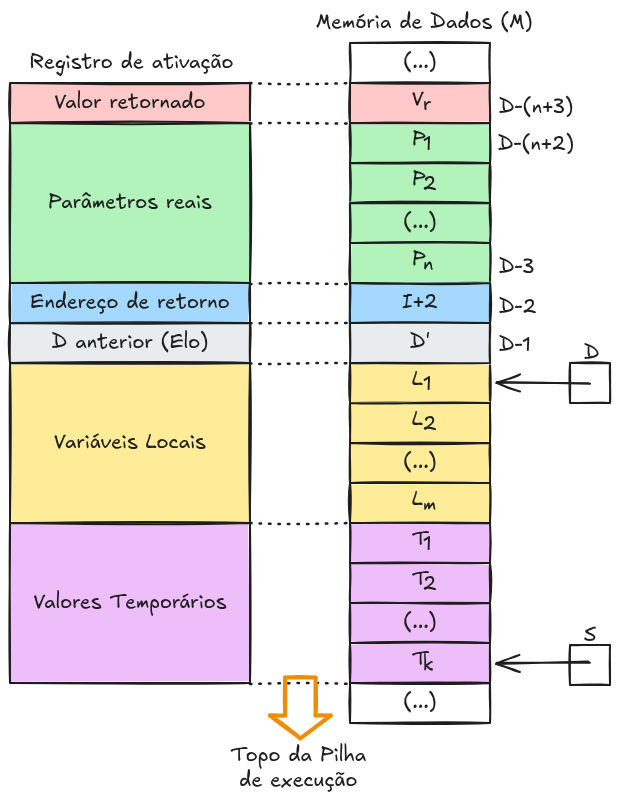
\includegraphics[width=0.6\linewidth,height=\textheight,keepaspectratio]{chapters/images/registro-ativacao-mvs.png}

}

\caption{\label{fig-registro-mvs}Registro de ativação da MVS}

\end{figure}%

A construção do registro de ativação na MVS começa com a reserva de uma
posição na pilha de execução para armazenar o valor de retorno (\(V_r\))
da rotina. Essa posição é necessária quando a rotina é uma função que
retorna um resultado ao seu chamador. No caso de um procedimento, que
não retorna valor, essa reserva não é necessária.

Em seguida, os valores dos \(n\) argumentos da chamada são empilhados,
na ordem estabelecida pela implementação da MVS. Esses valores serão
utilizados para inicializar os parâmetros formais (\(P_1\),
\(P_2\),\ldots,\(P_n\)) da rotina chamada. Dessa maneira, os argumentos
ficam disponíveis na pilha para serem acessados durante a execução da
rotina.

Antes de transferir o controle para a rotina, é necessário preservar as
informações que permitem retomar a execução no ponto em que a chamada
ocorreu. Para isso, o endereço de retorno (\(i+2\)) --- isto é, o
endereço da instrução que deverá ser executada após o término da rotina
--- é armazenado na pilha. Também é preservado o valor anterior do
registrador \texttt{D}, que representa o contexto da rotina chamadora.
Essas informações possibilitam restaurar o estado de execução anterior
quando a rotina terminar.

Após salvar essas informações, o registrador \texttt{D} é atualizado
para apontar para a posição da pilha que servirá como referência para o
novo registro de ativação. A partir desse ponto, são organizadas as
\(m\) variáveis locais (\(L_1\), \(L_2\),\ldots,\(L_m\)) e \(k\) os
valores temporários (\(T_1\), \(T_2\), \ldots, \(T_k\)) necessários à
execução da rotina. Os temporários são utilizados, por exemplo, para
armazenar resultados intermediários produzidos durante a avaliação de
expressões.

Ao final da execução da rotina, o processo de encerramento recupera as
informações preservadas durante a chamada. O valor do registrador
\texttt{D} correspondente ao contexto anterior pode ser recuperado da
posição \texttt{M{[}D-1{]}}, enquanto o endereço de retorno do programa
é recuperado da posição \texttt{M{[}D-2{]}}. Em seguida, a pilha é
ajustada para remover os elementos utilizados pelo registro de ativação,
incluindo os dados de controle e os demais valores associados à execução
da rotina.

Considerando que esses elementos ocupam as posições previstas pela
convenção de chamada da MVS, a remoção dos \texttt{n} valores dos
parâmetros mais as duas posições (\texttt{D} anterior e \texttt{i+2}),
isto é \texttt{n+2} valores, permite descartar os elementos do registro
de ativação sem eliminar o valor de retorno, quando houver. Assim, se a
rotina for uma função, o resultado permanece no topo da pilha,
disponível para ser utilizado pela expressão que contém a chamada. Se a
rotina for um procedimento, não há valor de retorno a preservar.

Esse mecanismo permite que chamadas de rotinas sejam executadas de
maneira aninhada e recursiva. Cada chamada estabelece um novo contexto
de execução, preservando as informações necessárias para que, ao
terminar, o controle retorne corretamente à rotina chamadora.

\subsection{Extensão da Máquina Virtual para Suporte a
Subprogramas}\label{extensuxe3o-da-muxe1quina-virtual-para-suporte-a-subprogramas}

A tradução de programas que utilizam funções e procedimentos exige que a
máquina virtual ofereça mecanismos para realizar chamadas de
subprogramas, transferir argumentos, preservar o contexto de execução e
retornar ao ponto em que a chamada foi realizada.

Para implementar essas funcionalidades, a máquina virtual MVS é
estendida com um conjunto de instruções específicas para manipulação de
variáveis locais, acesso indireto à memória, gerenciamento dos registros
de ativação e controle da execução de subprogramas.

A implementação utiliza a pilha de execução para armazenar informações
necessárias às chamadas de funções e procedimentos. Cada chamada
estabelece um novo contexto de execução, denominado \textbf{registro de
ativação}, que contém informações associadas à execução da rotina, como
parâmetros, variáveis locais e informações de controle.

Nesse mecanismo, três registradores desempenham papel fundamental:

\begin{itemize}
\tightlist
\item
  \texttt{s}: indica o topo da pilha de execução;
\item
  \texttt{d}: contém o endereço-base do registro de ativação corrente;
\item
  \texttt{i}: indica a posição da próxima instrução a ser executada no
  programa.
\end{itemize}

A memória da máquina virtual é representada por \texttt{M}, sendo
\texttt{M{[}x{]}} o conteúdo da posição de memória \texttt{x}.

\subsubsection{Novas instruções da
MVS}\label{novas-instruuxe7uxf5es-da-mvs}

A Tabela apresenta as instruções acrescentadas à máquina virtual para
permitir a tradução de funções e procedimentos.

\begin{longtable*}[]{|
  >{\raggedright\arraybackslash}p{(\linewidth - 6\tabcolsep - 4\arrayrulewidth) * \real{0.3333}}|
  >{\raggedright\arraybackslash}p{(\linewidth - 6\tabcolsep - 4\arrayrulewidth) * \real{0.3333}}|
  >{\raggedright\arraybackslash}p{(\linewidth - 6\tabcolsep - 4\arrayrulewidth) * \real{0.3333}}|}
\toprule\noalign{}
\begin{minipage}[b]{\linewidth}\smallskip
\raggedright
Instrução
\end{minipage} & \begin{minipage}[b]{\linewidth}\raggedright
Descrição
\end{minipage} & \begin{minipage}[b]{\linewidth}\raggedright
Microcódigo
\end{minipage} \\
\midrule\noalign{}
\endhead
\bottomrule\noalign{}
\endlastfoot
\texttt{CRVL\ n} & Carrega valor local & \(s \leftarrow s + 1\) \newline
\(M[s] \leftarrow M[d + n]\) \\
\midrule
\texttt{ARZL\ n} & Armazena valor em variável local &
\(M[d + n] \leftarrow M[s]\) \newline \(s \leftarrow s − 1\) \\
\midrule
\texttt{CREL\ n} & Carrega endereço local & \(s \leftarrow s + 1\)
\newline \(M[s] \leftarrow d + n\) \\
\midrule
\texttt{CREG\ n} & Carrega endereço global & \(s \leftarrow s + 1\)
\newline \(M[s] \leftarrow n\) \\
\midrule
\texttt{CRVI\ n} & Carrega valor indireto & \(s \leftarrow s + 1\)
\newline \(M[s] \leftarrow M[M[d + n]]\) \\
\midrule
\texttt{ARMI\ n} & Armazena valor indireto &
\(M[M[d + n]] \leftarrow M[s]\) \newline \(s \leftarrow s − 1\) \\
\midrule
\texttt{SVCP} & Salva contador do programa & \(s \leftarrow s + 1\)
\newline \(M[s] \leftarrow i + 2\) \\
\midrule
\texttt{ENSP} & Entrada em subprograma & \(s \leftarrow s + 1\) \newline
\(M[s] \leftarrow d\) \newline \(d \leftarrow s + 1\) \\
\midrule
\texttt{RTSP\ n} & Retorno de subprograma & \(d \leftarrow M[s]\)
\newline \(i \leftarrow M[s − 1]\) \newline
\(s \leftarrow s − (n + 2)\) \\
\end{longtable*}

\subsubsection{Descrição das
instruções}\label{descriuxe7uxe3o-das-instruuxe7uxf5es}

\paragraph{Manipulação de variáveis
locais}\label{manipulauxe7uxe3o-de-variuxe1veis-locais}

As instruções \texttt{CRVL}, \texttt{ARZL} e \texttt{CREL} permitem
acessar variáveis locais e seus endereços, utilizando o registrador
\texttt{d} como referência para o registro de ativação corrente.

\textbf{CRVL n -- Carrega valor local}

Obtém o conteúdo da variável localizada no deslocamento \texttt{n},
relativo ao endereço-base do registro de ativação, e coloca esse valor
no topo da pilha.

A instrução realiza duas operações: incrementa o ponteiro da pilha e
copia o conteúdo de \texttt{M{[}d+n{]}} para a nova posição.

\textbf{ARZL n -- Armazena valor local}

Armazena o valor que está no topo da pilha na posição correspondente à
variável local identificada pelo deslocamento \texttt{n}.

Após realizar a atribuição, decrementa o ponteiro da pilha, removendo o
valor utilizado.

\textbf{CREL n -- Carrega endereço local}

Obtém o endereço de uma variável local, calculado por \texttt{d+n}, e
coloca esse endereço no topo da pilha.

Diferentemente de \texttt{CRVL}, essa instrução não carrega o conteúdo
da variável, mas seu endereço. Isso permite implementar operações que
necessitam de referências a variáveis, como passagem de parâmetros por
referência.

\paragraph{Acesso a variáveis globais e
indiretas}\label{acesso-a-variuxe1veis-globais-e-indiretas}

As instruções \texttt{CREG}, \texttt{CRVI} e \texttt{ARMI} complementam
os mecanismos de acesso à memória.

\textbf{CREG n -- Carrega endereço global}

Coloca no topo da pilha o endereço \texttt{n} de uma variável global.

O endereço é armazenado diretamente na pilha, sem realizar a leitura do
conteúdo da posição de memória correspondente.

\textbf{CRVI n -- Carrega valor indireto}

Obtém o conteúdo de uma posição de memória cujo endereço está armazenado
na posição \texttt{M{[}d+n{]}}.

A operação utiliza dois níveis de acesso à memória:

\begin{enumerate}
\def\labelenumi{\arabic{enumi}.}
\tightlist
\item
  Obtém o endereço armazenado em \texttt{M{[}d+n{]}}.
\item
  Recupera o conteúdo da posição indicada por esse endereço e o coloca
  no topo da pilha.
\end{enumerate}

Essa instrução é particularmente útil para implementar o acesso a
parâmetros passados por referência.

\textbf{ARMI n -- Armazena valor indireto}

Realiza uma atribuição indireta. O valor que está no topo da pilha é
armazenado na posição de memória cujo endereço está armazenado em
\texttt{M{[}d+n{]}}.

Após a operação, o ponteiro da pilha é decrementado.

\paragraph{Controle de chamadas de
subprogramas}\label{controle-de-chamadas-de-subprogramas}

As instruções \texttt{SVCP}, \texttt{ENSP} e \texttt{RTSP} implementam o
mecanismo de chamada e retorno de funções e procedimentos.

\textbf{SVCP -- Salva contador do programa}

Salva na pilha o endereço da instrução que deverá ser executada após o
retorno do subprograma.

A operação utiliza \texttt{i+2}, considerando que a instrução
consecutiva é o desvio para o rótulo de entrada no subprograma, desta
forma o endereço de retorno do contador de programa é o endereço atual
\texttt{i} mais duas posições.

Esse endereço permite que a execução retorne ao ponto imediatamente
posterior à chamada.

\textbf{ENSP -- Entrada em subprograma}

Realiza a preparação do novo registro de ativação.

Inicialmente, salva na pilha o valor corrente de \texttt{d}, preservando
o endereço-base do registro de ativação do programa chamador. Em
seguida, atualiza \texttt{d}, estabelecendo a referência para o novo
registro de ativação.

Dessa maneira, cada chamada passa a possuir seu próprio contexto de
execução, permitindo a existência de chamadas aninhadas e recursivas.

\textbf{RTSP n -- Retorno de subprograma}

Realiza o encerramento da execução de uma função ou procedimento.

A instrução executa três operações:

\begin{enumerate}
\def\labelenumi{\arabic{enumi}.}
\tightlist
\item
  Recupera o endereço-base do registro de ativação anterior, restaurando
  o valor de \texttt{d}.
\item
  Recupera o endereço de retorno e o coloca no registrador \texttt{i},
  transferindo o controle para a instrução seguinte à chamada.
\item
  Atualiza o ponteiro da pilha, removendo os elementos associados à
  chamada, incluindo os parâmetros e as informações de controle,
  preservando o valor de retorno, se for o caso.
\end{enumerate}

O operando \texttt{n} representa a quantidade de parâmetros utilizada no
cálculo da desalocação. O termo \texttt{n+2} considera os parâmetros e
as duas posições de controle utilizadas pelo mecanismo de chamada:
endereço de retorno e endereço-base anterior.

\subsubsection{Funcionamento de uma chamada de
subprograma}\label{funcionamento-de-uma-chamada-de-subprograma}

O processo de chamada de uma função ou procedimento envolve a preparação
dos argumentos, o armazenamento das informações de controle e a criação
de um novo registro de ativação.

De maneira geral, o processo pode ser dividido nas seguintes etapas:

\begin{enumerate}
\def\labelenumi{\arabic{enumi}.}
\tightlist
\item
  \textbf{Preparação dos parâmetros:} os argumentos da chamada são
  avaliados e disponibilizados na pilha, conforme a convenção de
  passagem de parâmetros adotada pelo compilador.
\item
  \textbf{Salvamento do endereço de retorno:} a instrução \texttt{SVCP}
  armazena na pilha o endereço da próxima instrução a ser executada após
  o retorno.
\item
  \textbf{Criação do registro de ativação:} a instrução \texttt{ENSP}
  salva o endereço-base anterior e estabelece um novo valor para o
  registrador \texttt{d}.
\item
  \textbf{Execução do subprograma:} as instruções da rotina acessam seus
  parâmetros e variáveis locais utilizando os deslocamentos relativos a
  \texttt{d}.
\item
  \textbf{Retorno ao programa chamador:} a instrução \texttt{RTSP\ n}
  restaura o contexto anterior, recupera o endereço de retorno e libera
  o espaço ocupado pelos parâmetros e informações de controle.
\end{enumerate}

A utilização de registros de ativação na pilha permite que uma mesma
rotina seja chamada várias vezes, inclusive durante sua própria
execução. Essa característica é fundamental para implementar
procedimentos aninhados e algoritmos recursivos.

\subsection{Projeto de compilador com funções, procedimentos e passagem
de
parâmetros}\label{projeto-de-compilador-com-funuxe7uxf5es-procedimentos-e-passagem-de-paruxe2metros}

Nos capítulos anteriores, desenvolvemos os principais componentes de um
compilador para uma linguagem de programação simples: análise léxica,
análise sintática, análise semântica e geração de código para a Máquina
Virtual Simples (MVS). A linguagem implementada permite declarar
variáveis, realizar operações aritméticas e lógicas, executar comandos
de atribuição e utilizar estruturas de controle, como seleção e
repetição.

Embora esses recursos sejam suficientes para implementar algoritmos de
pequena complexidade, programas maiores exigem mecanismos que favoreçam
a modularização e o reaproveitamento de código. As funções e os
procedimentos atendem a essa necessidade ao permitir que um programa
seja dividido em unidades menores, cada uma responsável por realizar uma
tarefa específica.

Uma função executa um conjunto de comandos e devolve um resultado ao
programa que a chamou. Um procedimento também executa um conjunto de
comandos, mas não precisa retornar um valor como resultado de uma
expressão. Essa distinção permite organizar o programa em operações que
produzem valores e operações destinadas à realização de ações.

A utilização dessas construções introduz novos desafios para o
compilador. Além de reconhecer as declarações e as chamadas, é
necessário verificar a quantidade e os tipos dos parâmetros, controlar o
escopo dos identificadores e gerar instruções que permitam transferir a
execução entre o programa principal e os subprogramas.

Também é necessário estabelecer como os argumentos são transmitidos,
como as variáveis locais são armazenadas e como a execução retorna ao
ponto em que ocorreu a chamada. Essas responsabilidades envolvem tanto a
análise semântica quanto a geração de código e a organização da memória
durante a execução.

Neste capítulo, ampliaremos o projeto de compilador para contemplar
declarações de funções e procedimentos, chamadas de subprogramas e
diferentes formas de passagem de parâmetros. O objetivo é compreender
como os conceitos estudados anteriormente podem ser estendidos para
construir uma linguagem de programação com recursos de abstração e
modularização mais expressivos.

\subsection{Declaração de funções e
procedimentos}\label{declarauxe7uxe3o-de-funuxe7uxf5es-e-procedimentos}

Uma função ou um procedimento é uma unidade de programa identificada por
um nome e constituída, em geral, por uma lista de parâmetros,
declarações locais e um corpo de comandos.

Uma declaração de função especifica o tipo do valor que será devolvido.
Por exemplo:

\begin{Shaded}
\begin{Highlighting}[]
\KeywordTok{func} \KeywordTok{inteiro}\NormalTok{ soma(}\KeywordTok{inteiro}\NormalTok{ a }\KeywordTok{inteiro}\NormalTok{ b)}
\KeywordTok{inicio}
\NormalTok{    soma \textless{}{-} a + b}
\KeywordTok{fimfunc}
\end{Highlighting}
\end{Shaded}

A função \texttt{soma} recebe dois parâmetros inteiros, \texttt{a} e
\texttt{b}, e retorna a soma de seus valores. O tipo declarado após os
parâmetros indica que o resultado da função é inteiro.

Um procedimento pode ser declarado da seguinte forma:

\begin{Shaded}
\begin{Highlighting}[]
\KeywordTok{proc}\NormalTok{ imprime(}\KeywordTok{inteiro}\NormalTok{ valor)}
\KeywordTok{inicio}
    \KeywordTok{escreva}\NormalTok{ valor}
\KeywordTok{fimproc}
\end{Highlighting}
\end{Shaded}

Nesse exemplo, o procedimento \texttt{imprime} recebe um parâmetro
inteiro e apresenta seu valor. Não há um resultado a ser utilizado em
uma expressão, embora a execução do procedimento possa produzir efeitos,
como a escrita de dados.

Os exemplos utilizam uma notação ilustrativa para as declarações. A
sintaxe efetivamente adotada pelo compilador deverá ser definida pela
gramática da linguagem.

A inclusão dessas construções exige que o compilador reconheça novos
elementos sintáticos, entre eles:

\begin{itemize}
\tightlist
\item
  declarações de funções e procedimentos;
\item
  listas de parâmetros formais;
\item
  tipos de parâmetros e de retorno;
\item
  comandos de retorno;
\item
  chamadas de funções e procedimentos;
\item
  listas de argumentos efetivos.
\end{itemize}

Esses elementos precisam ser incorporados à gramática e associados a
regras semânticas que garantam a consistência das declarações e das
chamadas.

\subsection{Parâmetros formais e argumentos
efetivos}\label{paruxe2metros-formais-e-argumentos-efetivos}

Os parâmetros permitem que um subprograma receba informações do ambiente
que o invoca. Para compreender seu funcionamento, é importante
distinguir parâmetros formais de argumentos efetivos.

Os \textbf{parâmetros formais} são os identificadores declarados na
definição da função ou do procedimento. No exemplo anterior, \texttt{a}
e \texttt{b} são os parâmetros formais da função \texttt{soma}.

Os \textbf{argumentos efetivos} são os valores ou as expressões
fornecidos no momento da chamada. Por exemplo:

\begin{Shaded}
\begin{Highlighting}[]
\NormalTok{resultado \textless{}{-} soma(}\DecValTok{10}\NormalTok{, }\DecValTok{20}\NormalTok{)}
\end{Highlighting}
\end{Shaded}

Nessa chamada, \texttt{10} e \texttt{20} são os argumentos efetivos
correspondentes aos parâmetros formais \texttt{a} e \texttt{b}.

Durante a compilação, o compilador precisa verificar se a chamada
respeita a declaração do subprograma. No exemplo, a função espera dois
argumentos inteiros. Uma chamada com apenas um argumento ou com tipos
incompatíveis deve ser rejeitada, de acordo com as regras da linguagem.

A verificação envolve pelo menos três propriedades:

\begin{enumerate}
\def\labelenumi{\arabic{enumi}.}
\tightlist
\item
  \textbf{Quantidade de argumentos:} o número de argumentos deve ser
  compatível com o número de parâmetros declarados.
\item
  \textbf{Compatibilidade de tipos:} cada argumento deve ser compatível
  com o tipo do parâmetro correspondente.
\item
  \textbf{Ordem dos argumentos:} cada argumento deve ser associado ao
  parâmetro correto, conforme a posição ou as regras de associação
  definidas pela linguagem.
\end{enumerate}

Considere a seguinte chamada:

\begin{Shaded}
\begin{Highlighting}[]
\NormalTok{resultado \textless{}{-} soma(}\DecValTok{10}\NormalTok{)}
\end{Highlighting}
\end{Shaded}

Se a função exigir dois parâmetros, a chamada apresenta um erro
semântico, pois a quantidade de argumentos é insuficiente. Da mesma
forma, uma chamada como \texttt{soma(10,\ verdadeiro)} será inválida se
o segundo parâmetro exigir um valor inteiro e a linguagem não permitir a
conversão do valor lógico.

Essas verificações dependem das informações armazenadas na tabela de
símbolos. Portanto, a representação dos identificadores deverá ser
ampliada para registrar não apenas as variáveis, mas também as funções e
os procedimentos, incluindo suas listas de parâmetros e, no caso das
funções, o tipo de retorno.

\subsection{Passagem de parâmetros}\label{passagem-de-paruxe2metros}

A passagem de parâmetros determina como os argumentos fornecidos na
chamada são disponibilizados ao subprograma. Existem diferentes
mecanismos, e a escolha influencia tanto o comportamento do programa
quanto a implementação do compilador e da máquina virtual.

\subsubsection{Passagem por valor}\label{passagem-por-valor}

Na passagem por valor, o subprograma recebe uma cópia do valor do
argumento. Alterações realizadas no parâmetro formal não modificam
diretamente a variável utilizada na chamada.

Considere o procedimento:

\begin{Shaded}
\begin{Highlighting}[]
\KeywordTok{proc}\NormalTok{ incrementa(}\KeywordTok{inteiro}\NormalTok{ x)}
\KeywordTok{inicio}
\NormalTok{    x \textless{}{-} x + }\DecValTok{1}
\KeywordTok{fimproc}
\end{Highlighting}
\end{Shaded}

Suponha que o programa principal execute:

\begin{Shaded}
\begin{Highlighting}[]
\KeywordTok{inteiro}\NormalTok{ a}
\NormalTok{a \textless{}{-} }\DecValTok{5}
\NormalTok{incrementa(a)}
\end{Highlighting}
\end{Shaded}

Com passagem por valor, o procedimento recebe uma cópia do valor
\texttt{5}. Ao executar \texttt{x\ =\ x\ +\ 1}, o parâmetro local passa
a valer \texttt{6}, mas a variável \texttt{a} permanece com o valor
\texttt{5}.

Esse mecanismo exige que o compilador transmita o valor do argumento e
que o ambiente de execução disponibilize um espaço de armazenamento para
o parâmetro formal.

Na MVS, uma implementação possível consiste em avaliar o argumento,
colocar seu valor na pilha de execução e copiá-lo para a posição de
memória associada ao parâmetro formal durante a ativação do subprograma.

\subsubsection{Passagem por
referência}\label{passagem-por-referuxeancia}

Na passagem por referência, o parâmetro formal permite acessar a própria
variável associada ao argumento, em vez de receber apenas uma cópia de
seu valor. Dessa forma, as modificações realizadas no subprograma podem
ser observadas pelo programa que o chamou.

Considere o mesmo procedimento \texttt{incrementa}, agora com o
parâmetro declarado por referência:

\begin{Shaded}
\begin{Highlighting}[]
\KeywordTok{proc}\NormalTok{ incrementa(ref }\KeywordTok{inteiro}\NormalTok{ x)}
\KeywordTok{inicio}
\NormalTok{    x \textless{}{-} x + }\DecValTok{1}
\KeywordTok{fimproc}
\end{Highlighting}
\end{Shaded}

Ao executar:

\begin{Shaded}
\begin{Highlighting}[]
\KeywordTok{inteiro}\NormalTok{ a}
\NormalTok{a \textless{}{-} }\DecValTok{5}
\NormalTok{incrementa(a)}
\end{Highlighting}
\end{Shaded}

o procedimento acessa a variável original. Ao final da chamada,
\texttt{a} passa a valer \texttt{6}.

Para implementar esse mecanismo, o compilador precisa transmitir uma
referência à variável, normalmente representada por seu endereço. O
acesso ao parâmetro formal deve utilizar essa referência para ler ou
modificar o conteúdo da posição de memória correspondente.

Nem toda expressão pode ser utilizada como argumento de um parâmetro por
referência. Em uma implementação convencional, o argumento deve designar
uma posição de armazenamento válida, como uma variável. Uma constante ou
uma expressão aritmética, por exemplo, não pode ser tratada diretamente
como uma variável modificável sem regras adicionais.

\subsubsection{Comparação entre os
mecanismos}\label{comparauxe7uxe3o-entre-os-mecanismos}

\begin{longtable*}[]{|
  >{\raggedright\arraybackslash}p{(\linewidth - 6\tabcolsep - 4\arrayrulewidth) * \real{0.2544}}|
  >{\raggedright\arraybackslash}p{(\linewidth - 6\tabcolsep - 4\arrayrulewidth) * \real{0.3684}}|
  >{\raggedright\arraybackslash}p{(\linewidth - 6\tabcolsep - 4\arrayrulewidth) * \real{0.3772}}|}
\toprule\noalign{}
\begin{minipage}[b]{\linewidth}\smallskip
\raggedright
Característica
\end{minipage} & \begin{minipage}[b]{\linewidth}\raggedright
Passagem por valor
\end{minipage} & \begin{minipage}[b]{\linewidth}\raggedright
Passagem por referência
\end{minipage} \\
\midrule\noalign{}
\endhead
\bottomrule\noalign{}
\endlastfoot
Informação transmitida & Valor do argumento & Referência à variável \\
\midrule
Alteração do parâmetro formal & Não altera diretamente a variável
original & Pode alterar a variável original \\
\midrule
Armazenamento & Cópia do valor & Referência ou endereço \\
\midrule
Uso frequente & Fornecimento de dados & Consulta e modificação de dados
do chamador \\
\end{longtable*}

A linguagem implementada no projeto poderá adotar apenas passagem por
valor inicialmente e, posteriormente, incorporar passagem por
referência. Essa evolução permite compreender o mecanismo básico de
chamada antes de introduzir o tratamento de endereços e os efeitos das
alterações sobre as variáveis do programa principal.

\subsection{Modificações na
gramática}\label{modificauxe7uxf5es-na-gramuxe1tica}

As regras para declaração de funções e procedimentos pode ser incluído
da seguinte forma na gramática:

\begin{Shaded}
\begin{Highlighting}[]
\NormalTok{programa }
  \OperatorTok{:}\NormalTok{ cabecalho }
\NormalTok{    variaveis }
\NormalTok{    rotinas}
\NormalTok{    T\_INICIO lista\_comandos T\_FIM }

\NormalTok{cabecalho }
  \OperatorTok{:}\NormalTok{ T\_PROGRAMA T\_IDENTIF }\OperatorTok{;}

\NormalTok{rotinas }
  \OperatorTok{:} \CommentTok{/* vazia */}
  \OperatorTok{|}\NormalTok{ lista\_rotinas}\OperatorTok{;}

\NormalTok{lista\_rotinas}
  \OperatorTok{:}\NormalTok{ lista\_rotinas rotina}
  \OperatorTok{|}\NormalTok{ rotina}\OperatorTok{;}

\NormalTok{rotina }
  \OperatorTok{:}\NormalTok{ funcao }
  \OperatorTok{|}\NormalTok{ procedimento}\OperatorTok{;}

\NormalTok{funcao }
  \OperatorTok{:}\NormalTok{ T\_FUNC tipo T\_IDENTIF}
\NormalTok{    T\_ABRE lista\_parametros T\_FECHA}
\NormalTok{    variaveis}
\NormalTok{    T\_INICIO lista\_comandos T\_FIMFUNC }
    \OperatorTok{;}

\NormalTok{procedimento }
  \OperatorTok{:}\NormalTok{ T\_PROC T\_IDENTIF}
\NormalTok{    T\_ABRE lista\_parametros T\_FECHA}
\NormalTok{    variaveis}
\NormalTok{    T\_INICIO lista\_comandos T\_FIMPROC }
    \OperatorTok{;}

\NormalTok{lista\_parametros }
  \OperatorTok{:} \CommentTok{/* vazia */}
  \OperatorTok{|}\NormalTok{ lista\_parametros parametro}\OperatorTok{;}

\NormalTok{parametro }
  \OperatorTok{:}\NormalTok{ mecanismo tipo T\_IDENTIF }
    \OperatorTok{;}

\NormalTok{mecanismo }
  \OperatorTok{:} \CommentTok{/* vazia */} 
  \OperatorTok{|}\NormalTok{ T\_REF}\OperatorTok{;} 
\end{Highlighting}
\end{Shaded}

As chamadas de funções e procedimentos também são diferentes. As funções
são chamadas nas expressões e o procedimento é chamado como um comando.
As modificações na gramática então ficam:

\begin{Shaded}
\begin{Highlighting}[]
\OperatorTok{(...)}
\NormalTok{comando }
  \OperatorTok{:}\NormalTok{ entrada\_saida }
  \OperatorTok{|}\NormalTok{ repeticao }
  \OperatorTok{|}\NormalTok{ selecao }
  \OperatorTok{|}\NormalTok{ atribuicao}
  \OperatorTok{|}\NormalTok{ chamada\_procedimento }
  \OperatorTok{;}

\NormalTok{chamada\_procedimento}
  \OperatorTok{:}\NormalTok{ T\_IDENTIF T\_ABRE argumentos T\_FECHA}\OperatorTok{;}

\OperatorTok{(...)}

\NormalTok{termo }
  \OperatorTok{:}\NormalTok{ T\_IDENTIF }
  \OperatorTok{|}\NormalTok{ T\_IDENTIF T\_ABRE argumentos T\_FECHA}\OperatorTok{;}

\OperatorTok{(...)}

\NormalTok{argumentos }
  \OperatorTok{:} \CommentTok{/* vazia */}
  \OperatorTok{|}\NormalTok{ lista\_argumentos }\OperatorTok{;}

\NormalTok{lista\_argumentos }
  \OperatorTok{:}\NormalTok{ lista\_argumentos expressao }
  \OperatorTok{|}\NormalTok{ expressao}
  \OperatorTok{;}
\end{Highlighting}
\end{Shaded}

\subsection{Escopo e tabela de
símbolos}\label{escopo-e-tabela-de-suxedmbolos}

A introdução de funções e procedimentos exige ampliar a tabela de
símbolos utilizada nos projetos anteriores. Até aqui, cada identificador
armazenava informações como nome, endereço e tipo. Com os novos
recursos, o compilador deverá distinguir variáveis, funções e
procedimentos.

Para uma função, por exemplo, a tabela poderá armazenar:

\begin{itemize}
\tightlist
\item
  nome da função;
\item
  categoria do identificador;
\item
  tipo do valor retornado;
\item
  quantidade de parâmetros;
\item
  tipos dos parâmetros;
\item
  mecanismos de passagem dos parâmetros;
\item
  informações necessárias à geração do código da chamada.
\end{itemize}

Para um procedimento, as informações serão semelhantes, exceto pelo tipo
de retorno, que não representa um valor utilizado em expressões.

Também será necessário tratar o escopo dos identificadores. Uma variável
declarada dentro de uma função pode ter existência e visibilidade
restritas ao corpo dessa função. Outra função poderá declarar uma
variável com o mesmo nome, sem que isso implique necessariamente um
conflito.

Para representar esses contextos, uma solução consiste em manter uma
tabela de símbolos associada a cada escopo ou utilizar uma tabela
organizada em níveis. Quando o compilador entra em uma função ou
procedimento, cria ou ativa o escopo correspondente. Ao terminar o
processamento da declaração, encerra esse escopo, preservando as
informações globais que continuam válidas.

Essa organização evita que parâmetros e variáveis locais sejam
confundidos com identificadores de outras unidades do programa. Além
disso, permite detectar usos de variáveis fora de seu escopo e chamadas
a funções ou procedimentos não declarados, conforme as regras da
linguagem.

\subsection{Ativação de funções e
procedimentos}\label{ativauxe7uxe3o-de-funuxe7uxf5es-e-procedimentos}

Durante a execução, cada chamada de função ou procedimento cria uma nova
ativação do subprograma. Essa ativação reúne as informações necessárias
para executar o corpo do subprograma e retornar ao ponto de chamada.

Uma implementação convencional utiliza um registro de ativação, também
conhecido como quadro de ativação (\emph{activation record}). Ele pode
conter:

\begin{itemize}
\tightlist
\item
  parâmetros recebidos;
\item
  variáveis locais;
\item
  endereço de retorno;
\item
  informações de controle da chamada;
\item
  espaço para o resultado da função, quando necessário.
\end{itemize}

A organização exata depende da máquina virtual e da convenção de chamada
adotada. Em uma máquina baseada em pilha, os registros de ativação podem
ser organizados em uma pilha de chamadas, permitindo que uma função
invoque outra e que chamadas recursivas mantenham dados independentes
para cada ativação.

Considere:

\begin{Shaded}
\begin{Highlighting}[]
\KeywordTok{func} \KeywordTok{inteiro}\NormalTok{ quadrado(}\KeywordTok{inteiro}\NormalTok{ x)}
\KeywordTok{inicio}
\NormalTok{    quadrado \textless{}{-} x * x}
\KeywordTok{fimfunc}
\end{Highlighting}
\end{Shaded}

Quando o programa executa \texttt{quadrado(5)}, o ambiente de execução
disponibiliza o parâmetro \texttt{x}, executa a multiplicação e devolve
o resultado \texttt{25} ao ponto da chamada.

Se a função \texttt{quadrado} for chamada novamente antes de a execução
anterior terminar, cada ativação deverá preservar seu próprio valor de
\texttt{x} e seu próprio endereço de retorno. Esse requisito é
fundamental para permitir recursão.

No compilador para a MVS, será necessário definir como os parâmetros e
as variáveis locais serão organizados na memória e como o endereço de
retorno será preservado. Caso a máquina virtual não ofereça diretamente
essas operações, será necessário implementar uma convenção de chamada
por meio das instruções disponíveis ou ampliar o conjunto de instruções
da máquina.

\subsection{Geração de código para
chamadas}\label{gerauxe7uxe3o-de-cuxf3digo-para-chamadas}

A geração de código deve traduzir a chamada de uma função ou
procedimento em uma sequência de operações que prepare os argumentos,
transfira a execução ao subprograma e permita o retorno ao chamador.

Para uma chamada como:

\begin{Shaded}
\begin{Highlighting}[]
\NormalTok{resultado \textless{}{-} soma(}\DecValTok{10} \DecValTok{20}\NormalTok{)}
\end{Highlighting}
\end{Shaded}

o compilador deverá gerar código que, conceitualmente, realize as
seguintes operações:

\begin{enumerate}
\def\labelenumi{\arabic{enumi}.}
\tightlist
\item
  Avalie os argumentos na ordem definida pela linguagem.
\item
  Disponibilize os valores ou referências aos parâmetros formais.
\item
  Preserve as informações necessárias para retornar ao ponto da chamada.
\item
  Transfira o controle para o código da função.
\item
  Execute o corpo da função e obtenha o resultado.
\item
  Retorne ao chamador e disponibilize o valor retornado para completar a
  atribuição.
\end{enumerate}

O código concreto dependerá das instruções oferecidas pela MVS. Se a
máquina virtual possuir instruções específicas para chamada e retorno,
elas poderão ser utilizadas diretamente. Caso contrário, será necessário
construir uma sequência equivalente usando desvios, pilha e posições de
memória reservadas para o controle das chamadas.

É importante distinguir a chamada do subprograma de sua declaração. A
declaração define o corpo da função ou do procedimento, enquanto a
chamada transfere a execução para esse corpo em um ponto específico do
programa.

Para evitar que o programa execute o corpo de uma função apenas por ele
aparecer no arquivo gerado, o compilador deverá organizar os rótulos e
desvios de maneira que a execução normal passe pelo programa principal e
alcance cada subprograma somente quando houver uma chamada
correspondente.

\subsubsection{Retorno de funções}\label{retorno-de-funuxe7uxf5es}

Uma função precisa devolver um valor compatível com o tipo declarado. O
comando de atribuição para variável com o nome da função pode ser
utilizado para indicar o resultado:

\begin{Shaded}
\begin{Highlighting}[]
\KeywordTok{func} \KeywordTok{inteiro}\NormalTok{ soma(}\KeywordTok{inteiro}\NormalTok{ a, }\KeywordTok{inteiro}\NormalTok{ b)}
\KeywordTok{inicio}
\NormalTok{    soma \textless{}{-} a + b}
\KeywordTok{fimfunc}
\end{Highlighting}
\end{Shaded}

O compilador deverá verificar se a expressão retornada é compatível com
o tipo da função. Também deverá definir as regras para funções que
terminam sem executar um comando de retorno, incluindo a possibilidade
de rejeitar essas situações durante a análise semântica.

Na geração de código, o resultado poderá ser colocado em uma posição da
pilha, em um espaço reservado no registro de ativação ou em outro local
definido pela convenção de chamada. A instrução de retorno deverá
restaurar o fluxo de execução e disponibilizar o valor ao chamador.

\subsubsection{Retorno de procedimentos}\label{retorno-de-procedimentos}

Um procedimento não precisa devolver um valor para ser utilizado em uma
expressão. Seu término deve apenas permitir que a execução retorne ao
ponto da chamada.

Por exemplo:

\begin{Shaded}
\begin{Highlighting}[]
\KeywordTok{proc}\NormalTok{ mensagem()}
\KeywordTok{inicio}
    \KeywordTok{escreva} \DecValTok{1}
\KeywordTok{fimproc}
\end{Highlighting}
\end{Shaded}

Uma chamada a \texttt{mensagem()} executa o corpo do procedimento e, ao
final, retorna ao comando seguinte. O compilador deverá garantir que o
retorno não deixe valores indevidos na pilha e que a memória temporária
utilizada durante a ativação seja liberada de acordo com a convenção
adotada.

\subsection{Exemplos de tradução}\label{exemplos-de-traduuxe7uxe3o}

Apresentamos, a seguir, alguns exemplos de tradução que podem servir de
referência para o desenvolvimento do compilador, contemplando a tradução
de procedimentos e funções com passagem de parâmetros por valor ou por
referência. Para ilustrar esse processo, as imagens seguintes apresentam
os valores registrados na tabela de símbolos durante a declaração das
rotinas e após sua conclusão, quando o compilador retorna ao contexto
global.

\textbf{Exemplo 1}

\begin{Shaded}
\begin{Highlighting}[]
\KeywordTok{programa}\NormalTok{ parametros}
  \KeywordTok{proc}\NormalTok{ somatudo(}\KeywordTok{inteiro}\NormalTok{ a }
                 \KeywordTok{inteiro}\NormalTok{ b }
                 \KeywordTok{inteiro}\NormalTok{ c }
                 \KeywordTok{inteiro}\NormalTok{ d)}
  \KeywordTok{inicio}
    \KeywordTok{escreva}\NormalTok{ a + b + c + d}
  \KeywordTok{fimproc}
  
\KeywordTok{inicio}
\NormalTok{  somatudo(}\DecValTok{10} \DecValTok{3} \DecValTok{4} \DecValTok{8}\NormalTok{)}
\KeywordTok{fimprograma}
\end{Highlighting}
\end{Shaded}

A Figura Figura~\ref{fig-exemplo1} ilustra o comportamento da tabela de
símbolos durante a compilação da declaração do procedimento
\texttt{somatudo}. Inicialmente, ao identificar a declaração da rotina,
o compilador registra uma entrada correspondente ao procedimento e, em
seguida, inclui os seus quatro parâmetros (\texttt{a}, \texttt{b},
\texttt{c} e \texttt{d}). Para cada parâmetro, são armazenadas
informações como nome, tipo, endereço relativo, escopo, categoria e
mecanismo de passagem. Nesse exemplo, todos os parâmetros são do tipo
inteiro e são passados por valor (\texttt{val}).

Durante a compilação do corpo do procedimento, os parâmetros permanecem
registrados na tabela de símbolos e associados ao escopo local da rotina
(\texttt{L}). Os endereços relativos atribuídos aos parâmetros são
utilizados pelo compilador para orientar o acesso aos respectivos
valores durante a execução. Além disso, a entrada do procedimento contém
informações sobre sua identificação, seu rótulo (\texttt{L1}) para onde
deve ser desviada a execução na chamada da rotina, a quantidade de
parâmetros (\texttt{npar\ =\ 4}) e suas respectivas características de
passagem, representadas na coluna lista de parâmetros \texttt{lpar}
(onde \texttt{i} ou \texttt{l} indica o tipo do parâmetro, inteiro ou
lógico, respectivamente e \texttt{v} ou \texttt{r}, indica o tipo de
passagem, valor ou referência, respectivamente).

Após a compilação do procedimento, ao encontrar a instrução
\texttt{fimproc}, o compilador encerra o escopo local e remove da tabela
de símbolos as entradas correspondentes aos parâmetros. Entretanto, a
entrada do procedimento é preservada no escopo global (\texttt{G}),
mantendo as informações necessárias para sua identificação e posterior
utilização no restante do programa. Dessa forma, quando o compilador
encontra a chamada \texttt{somatudo(10\ 3\ 4\ 8)}, pode consultar a
tabela de símbolos para verificar a existência da rotina, a quantidade
de argumentos esperados e as características de passagem dos parâmetros,
orientando a geração do código correspondente à chamada.

\begin{figure}

\centering{

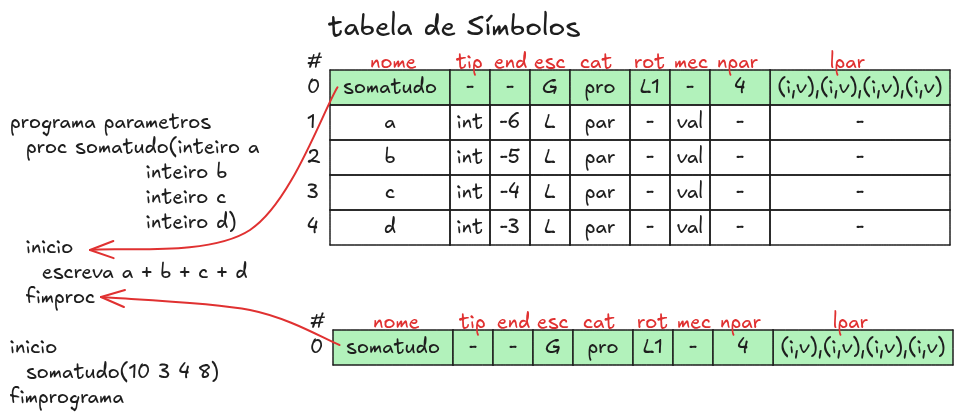
\includegraphics[width=0.9\linewidth,height=\textheight,keepaspectratio]{chapters/images/exemplo1.png}

}

\caption{\label{fig-exemplo1}Exemplo de compilação de um procedimento}

\end{figure}%

O resultado da compilação é:

\begin{Shaded}
\begin{Highlighting}[]
    \KeywordTok{INPP}
    \KeywordTok{DSVS}    \FunctionTok{L0}
\FunctionTok{L1}  \KeywordTok{ENSP}
    \KeywordTok{CRVL}\NormalTok{    {-}}\DecValTok{6}
    \KeywordTok{CRVL}\NormalTok{    {-}}\DecValTok{5}
    \KeywordTok{SOMA}
    \KeywordTok{CRVL}\NormalTok{    {-}}\DecValTok{4}
    \KeywordTok{SOMA}
    \KeywordTok{CRVL}\NormalTok{    {-}}\DecValTok{3}
    \KeywordTok{SOMA}
    \KeywordTok{ESCR}
    \KeywordTok{RTSP}    \DecValTok{4}
\FunctionTok{L0}  \KeywordTok{NADA}
    \KeywordTok{CRCT}    \DecValTok{10}
    \KeywordTok{CRCT}    \DecValTok{3}
    \KeywordTok{CRCT}    \DecValTok{4}
    \KeywordTok{CRCT}    \DecValTok{8}
    \KeywordTok{SVCP}
    \KeywordTok{DSVS}    \FunctionTok{L1}
    \KeywordTok{FIMP}
\end{Highlighting}
\end{Shaded}

O código apresentado corresponde à tradução do programa que declara e
utiliza o procedimento \texttt{somatudo}, responsável por receber quatro
parâmetros inteiros, calcular a soma de seus valores e apresentar o
resultado na saída padrão. A tradução é organizada em duas partes: a
implementação do procedimento e o programa principal, que realiza sua
chamada.

\emph{Inicialização e desvio para o programa principal}

\begin{Shaded}
\begin{Highlighting}[]
    \KeywordTok{INPP}
    \KeywordTok{DSVS}    \FunctionTok{L0}
\end{Highlighting}
\end{Shaded}

A instrução \texttt{INPP} inicializa a execução do programa, preparando
as estruturas necessárias para o seu funcionamento. Em seguida,
\texttt{DSVS\ L0} realiza um desvio incondicional para o rótulo
\texttt{L0}, evitando que o fluxo de execução passe diretamente pelo
código do procedimento. Essa estratégia permite que a execução comece
pelo programa principal, deixando o corpo do procedimento disponível
para ser executado somente quando ocorrer uma chamada.

\emph{Implementação do procedimento \texttt{somatudo}}

\begin{Shaded}
\begin{Highlighting}[]
\FunctionTok{L1}  \KeywordTok{ENSP}
    \KeywordTok{CRVL}\NormalTok{    {-}}\DecValTok{6}
    \KeywordTok{CRVL}\NormalTok{    {-}}\DecValTok{5}
    \KeywordTok{SOMA}
    \KeywordTok{CRVL}\NormalTok{    {-}}\DecValTok{4}
    \KeywordTok{SOMA}
    \KeywordTok{CRVL}\NormalTok{    {-}}\DecValTok{3}
    \KeywordTok{SOMA}
    \KeywordTok{ESCR}
    \KeywordTok{RTSP}    \DecValTok{4}
\end{Highlighting}
\end{Shaded}

O rótulo \texttt{L1} identifica o ponto de entrada do procedimento. A
instrução \texttt{ENSP} inicia a execução da rotina, preparando o
ambiente necessário para seu processamento.

As instruções \texttt{CRVL} recuperam os valores dos parâmetros
armazenados na memória, utilizando seus endereços relativos. Nesse
exemplo, os deslocamentos \texttt{-6}, \texttt{-5}, \texttt{-4} e
\texttt{-3} correspondem, respectivamente, aos parâmetros \texttt{a},
\texttt{b}, \texttt{c} e \texttt{d}.

A instrução \texttt{SOMA} realiza a adição dos dois valores disponíveis
no topo da pilha. Dessa maneira, o código executa sucessivamente as
operações necessárias para calcular:

\begin{Shaded}
\begin{Highlighting}[]
\NormalTok{a+b+c+d}
\end{Highlighting}
\end{Shaded}

Após o cálculo, a instrução \texttt{ESCR} apresenta o resultado na saída
padrão. Finalmente, \texttt{RTSP\ 4} encerra a execução do procedimento
e retorna ao ponto de chamada, considerando a quantidade de quatro
parâmetros utilizados pela rotina.

\emph{Execução do programa principal}

\begin{Shaded}
\begin{Highlighting}[]
\FunctionTok{L0}  \KeywordTok{NADA}
    \KeywordTok{CRCT}    \DecValTok{10}
    \KeywordTok{CRCT}    \DecValTok{3}
    \KeywordTok{CRCT}    \DecValTok{4}
    \KeywordTok{CRCT}    \DecValTok{8}
    \KeywordTok{SVCP}
    \KeywordTok{DSVS}    \FunctionTok{L1}
    \KeywordTok{FIMP}
\end{Highlighting}
\end{Shaded}

O rótulo \texttt{L0} marca o início do programa principal. A instrução
\texttt{NADA} não realiza nenhuma operação, sendo utilizada apenas como
referência para o desvio efetuado anteriormente.

As quatro instruções \texttt{CRCT} empilham os valores constantes
\texttt{10}, \texttt{3}, \texttt{4} e \texttt{8}, que serão utilizados
como argumentos na chamada do procedimento. Em seguida, \texttt{SVCP}
salva o endereço da instrução que deverá ser executada quando a chamada
do procedimento for encerrado e a execução retornar para o programa
principal, de acordo com a convenção de passagem de parâmetros adotada
pela máquina.

A instrução \texttt{DSVS\ L1} transfere o fluxo de execução para o
endereço identificado pelo rótulo \texttt{L1}, iniciando a execução do
procedimento \texttt{somatudo}. Após a conclusão da rotina, a instrução
\texttt{RTSP\ 4} realiza o retorno ao programa principal, permitindo que
a execução prossiga na instrução seguinte à chamada, que, nesse caso, é
\texttt{FIMP}.

Por fim, \texttt{FIMP} indica o término da execução do programa.

\emph{Resultado da execução}

Considerando a chamada:

\begin{Shaded}
\begin{Highlighting}[]
\VariableTok{somatudo}\NormalTok{(}\DecValTok{10} \DecValTok{3} \DecValTok{4} \DecValTok{8}\NormalTok{)}
\end{Highlighting}
\end{Shaded}

o procedimento recebe os valores correspondentes aos seus quatro
parâmetros e realiza as seguintes operações:

\[ 10+3=13 \]

\[ 13+4=17 \]

\[ 17+8=25 \]

Saída esperada

\begin{verbatim}
25
\end{verbatim}

Esse exemplo demonstra como o compilador traduz a declaração de um
procedimento e sua respectiva chamada, incluindo a organização dos
parâmetros na pilha, o acesso aos valores por meio de endereços
relativos, o desvio para a rotina e o retorno ao fluxo de execução do
programa principal.

\textbf{Exemplo 2}

\begin{Shaded}
\begin{Highlighting}[]
\KeywordTok{programa}\NormalTok{ rotina}
  \KeywordTok{inteiro}\NormalTok{ x y}
  
  \KeywordTok{proc}\NormalTok{ p(ref }\KeywordTok{inteiro}\NormalTok{ s)}
    \KeywordTok{inteiro}\NormalTok{ z}
  \KeywordTok{inicio}
    \KeywordTok{se}\NormalTok{ s \textgreater{} }\DecValTok{1}
       \KeywordTok{entao}\NormalTok{ y \textless{}{-} }\DecValTok{1}
       \KeywordTok{senao}\NormalTok{ z \textless{}{-} s {-} }\DecValTok{1}
\NormalTok{             p(z)}
\NormalTok{             y \textless{}{-} y * s}
    \KeywordTok{fimse}
  \KeywordTok{fimproc}

\KeywordTok{inicio}
\NormalTok{   x \textless{}{-} }\DecValTok{4}
\NormalTok{   p(x)}
   \KeywordTok{escreva}\NormalTok{ x}
   \KeywordTok{escreva}\NormalTok{ y}
\KeywordTok{fimprograma}
\end{Highlighting}
\end{Shaded}

A Figura Figura~\ref{fig-exemplo2} apresenta a organização da tabela de
símbolos durante a compilação da declaração do procedimento \texttt{p},
que possui um parâmetro passado por referência e uma variável local. O
exemplo permite observar como o compilador registra as variáveis
globais, as informações da rotina, os parâmetros e as variáveis locais,
bem como o comportamento da tabela de símbolos após o encerramento da
declaração do procedimento.

\emph{Variáveis globais e declaração do procedimento}

Inicialmente, o programa declara duas variáveis inteiras, \texttt{x} e
\texttt{y}, que são registradas na tabela de símbolos com os seguintes
valores:

\begin{itemize}
\tightlist
\item
  \texttt{x}: variável do tipo inteiro, com endereço real \texttt{0},
  escopo global (\texttt{G}) e categoria \texttt{var}.
\item
  \texttt{y}: variável do tipo inteiro, com endereço real \texttt{1},
  escopo global (\texttt{G}) e categoria \texttt{var}.
\end{itemize}

Essas variáveis permanecem disponíveis durante toda a execução do
programa, inclusive dentro dos procedimentos e funções declarados.

Na sequência, o compilador identifica a declaração do procedimento
\texttt{p}, cujo parâmetro \texttt{s} é do tipo inteiro e utiliza
passagem por referência. A entrada correspondente ao procedimento
apresenta as seguintes informações:

\begin{itemize}
\tightlist
\item
  \textbf{nome}: identificação da rotina (\texttt{p}).
\item
  \textbf{tipo}: não se aplica, pois se trata de um procedimento, que
  não possui valor de retorno.
\item
  \textbf{esc}: escopo global (\texttt{G}), indicando que a rotina foi
  declarada no nível global do programa.
\item
  \textbf{cat}: categoria \texttt{pro}, identificando uma declaração de
  procedimento.
\item
  \textbf{rot}: rótulo \texttt{L1}, que identifica o endereço de entrada
  do código gerado para a rotina.
\item
  \textbf{npar}: quantidade de parâmetros, nesse caso, \texttt{1}.
\item
  \textbf{lpar}: informações sobre os parâmetros, representadas por
  \texttt{(i,r)}, indicando que o parâmetro é do tipo inteiro
  (\texttt{i}) e utiliza passagem por referência (\texttt{r}).
\end{itemize}

\emph{Parâmetros e variáveis locais do procedimento}

Durante a compilação do corpo do procedimento, o compilador registra
também os identificadores pertencentes ao escopo local (\texttt{L}).
Nesse exemplo, são registradas duas entradas:

\begin{itemize}
\tightlist
\item
  \texttt{s}: parâmetro do tipo inteiro, com endereço relativo
  \texttt{-3}, escopo local (\texttt{L}), categoria \texttt{par} e
  mecanismo de passagem \texttt{ref}, indicando que seu valor é acessado
  por referência. O endereço relativo negativo decorre da convenção de
  organização dos parâmetros no ambiente de execução da MVS.
\item
  \texttt{z}: variável local do tipo inteiro, com endereço relativo
  \texttt{0}, escopo local (\texttt{L}) e categoria \texttt{var}. Como
  se trata de uma variável declarada dentro do procedimento, seu
  armazenamento pertence ao ambiente de execução da rotina.
\end{itemize}

É importante observar que, embora \texttt{s} seja um parâmetro formal,
ele também é registrado na tabela de símbolos como uma entidade
pertencente ao escopo local do procedimento. A informação sobre o
mecanismo de passagem é armazenada separadamente, permitindo ao
compilador distinguir parâmetros passados por valor daqueles passados
por referência.

\emph{Tabela de símbolos após o encerramento do procedimento}

A segunda tabela apresenta a situação após a compilação da declaração do
procedimento, quando o compilador encontra a instrução \texttt{fimproc}.

Nesse momento, as entradas correspondentes ao parâmetro \texttt{s} e à
variável local \texttt{z} são removidas, pois pertencem ao escopo local
da rotina, que foi encerrado.

Entretanto, permanecem na tabela as entradas referentes às variáveis
globais \texttt{x} e \texttt{y} e ao procedimento \texttt{p}. A entrada
do procedimento conserva suas informações de identificação, seu rótulo
de código (\texttt{L1}), a quantidade de parâmetros
(\texttt{npar\ =\ 1}) e suas características de passagem
(\texttt{par\ =\ (i,r)}).

Essa preservação é necessária porque o procedimento poderá ser chamado
em diferentes pontos do programa, e o compilador precisa consultar suas
informações para verificar a quantidade, os tipos e os mecanismos de
passagem dos argumentos utilizados nas chamadas.

\emph{A passagem por referência}

O exemplo também ilustra a diferença entre o registro de um parâmetro
passado por referência e o de uma variável local. Enquanto o parâmetro
\texttt{s} possui o mecanismo \texttt{ref} e utiliza um endereço
relativo negativo, a variável \texttt{z} é armazenada diretamente no
ambiente local do procedimento.

Essa distinção é particularmente importante para a geração de código.
Quando o procedimento modifica o parâmetro \texttt{s}, a alteração deve
refletir diretamente na variável utilizada como argumento na chamada.
Por outro lado, as operações realizadas sobre \texttt{z} afetam apenas a
variável local da execução corrente do procedimento.

Assim, a tabela de símbolos mantém as informações necessárias para que o
compilador gere corretamente o código de acesso às variáveis,
respeitando seus escopos e os mecanismos de passagem de parâmetros.

Observação sobre o exemplo: na chamada \texttt{p(x)}, o parâmetro formal
\texttt{s} recebe uma referência à variável global \texttt{x}. Portanto,
quando o procedimento executa \texttt{s\ \textless{}-\ 1}, está
modificando diretamente o conteúdo de \texttt{x}. Essa característica
permite ilustrar o efeito da passagem por referência sobre as variáveis
do programa chamador.

\begin{figure}

\centering{

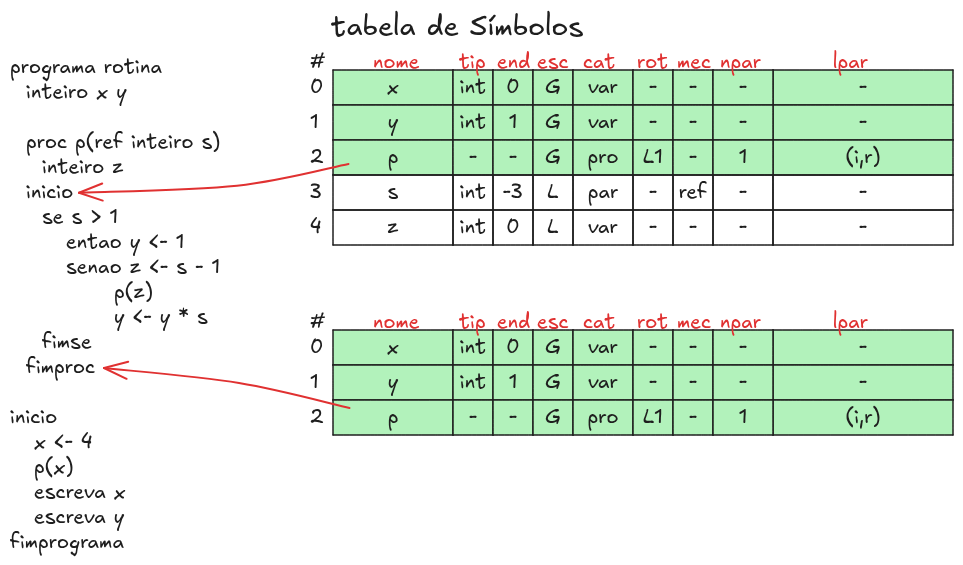
\includegraphics[width=0.9\linewidth,height=\textheight,keepaspectratio]{chapters/images/exemplo2.png}

}

\caption{\label{fig-exemplo2}Exemplo de compilação de rotina com
passagem de parâmetro por referência}

\end{figure}%

E o resultado do código compilado para MVS é:

\begin{Shaded}
\begin{Highlighting}[]
    \KeywordTok{INPP}
    \KeywordTok{AMEM}    \DecValTok{2}
    \KeywordTok{DSVS}    \FunctionTok{L0}
\FunctionTok{L1}  \KeywordTok{ENSP}
    \KeywordTok{AMEM}    \DecValTok{1}
    \KeywordTok{CRVI}\NormalTok{    {-}}\DecValTok{3}
    \KeywordTok{CRCT}    \DecValTok{1}
    \KeywordTok{CMMA}
    \KeywordTok{DSVF}    \FunctionTok{L2}
    \KeywordTok{CRCT}    \DecValTok{1}
    \KeywordTok{ARZG}    \DecValTok{1}
    \KeywordTok{DSVS}    \FunctionTok{L3}
\FunctionTok{L2}  \KeywordTok{NADA}
    \KeywordTok{CRVI}\NormalTok{    {-}}\DecValTok{3}
    \KeywordTok{CRCT}    \DecValTok{1}
    \KeywordTok{SUBT}
    \KeywordTok{ARZL}    \DecValTok{0}
    \KeywordTok{CREL}    \DecValTok{0}
    \KeywordTok{SVCP}
    \KeywordTok{DSVS}    \FunctionTok{L1}
    \KeywordTok{CRVG}    \DecValTok{1}
    \KeywordTok{CRVI}\NormalTok{    {-}}\DecValTok{3}
    \KeywordTok{MULT}
    \KeywordTok{ARZG}    \DecValTok{1}
\FunctionTok{L3}  \KeywordTok{NADA}
    \KeywordTok{DMEM}    \DecValTok{1}
    \KeywordTok{RTSP}    \DecValTok{1}
\FunctionTok{L0}  \KeywordTok{NADA}
    \KeywordTok{CRCT}    \DecValTok{4}
    \KeywordTok{ARZG}    \DecValTok{0}
    \KeywordTok{CREG}    \DecValTok{0}
    \KeywordTok{SVCP}
    \KeywordTok{DSVS}    \FunctionTok{L1}
    \KeywordTok{CRVG}    \DecValTok{0}
    \KeywordTok{ESCR}
    \KeywordTok{CRVG}    \DecValTok{1}
    \KeywordTok{ESCR}
    \KeywordTok{DMEM}    \DecValTok{2}
    \KeywordTok{FIMP}
\end{Highlighting}
\end{Shaded}

O código apresentado corresponde à tradução para a máquina virtual MVS
de um programa que declara um procedimento recursivo \texttt{p}, cujo
parâmetro inteiro \texttt{s} é passado por referência. O procedimento
também utiliza uma variável local \texttt{z} e uma variável global
\texttt{y}.

A implementação contém uma estrutura condicional que verifica se o
parâmetro \texttt{s} é maior que um. Caso a condição seja verdadeira,
atribui o valor um à variável global \texttt{y}. Caso contrário, calcula
um novo valor para \texttt{z}, realiza uma chamada recursiva e, após o
retorno, multiplica o resultado armazenado em \texttt{y} pelo valor de
\texttt{s}.

\emph{Inicialização do programa}

\begin{Shaded}
\begin{Highlighting}[]
    \KeywordTok{INPP}
    \KeywordTok{AMEM}    \DecValTok{2}
    \KeywordTok{DSVS}    \FunctionTok{L0}
\end{Highlighting}
\end{Shaded}

A instrução \texttt{INPP} inicializa a execução do programa. Em seguida,
\texttt{AMEM\ 2} reserva duas posições de memória para as variáveis
globais \texttt{x} e \texttt{y}. A instrução \texttt{DSVS\ L0} realiza
um desvio incondicional para o início do programa principal, evitando
que a execução passe diretamente pelo código do procedimento.

\emph{Implementação do procedimento recursivo}

O procedimento é identificado pelo rótulo \texttt{L1} e possui um
parâmetro inteiro \texttt{s}, passado por referência, e uma variável
local \texttt{z}.

\begin{Shaded}
\begin{Highlighting}[]
\FunctionTok{L1}  \KeywordTok{ENSP}
    \KeywordTok{AMEM}    \DecValTok{1}
    \KeywordTok{CRVI}\NormalTok{    {-}}\DecValTok{3}
    \KeywordTok{CRCT}    \DecValTok{1}
    \KeywordTok{CMMA}
    \KeywordTok{DSVF}    \FunctionTok{L2}
\end{Highlighting}
\end{Shaded}

A instrução \texttt{ENSP} inicia a execução do procedimento, preparando
o ambiente necessário para a chamada. Em seguida, \texttt{AMEM\ 1}
reserva uma posição de memória para a variável local \texttt{z}.

As instruções \texttt{CRVI\ -3} e \texttt{CRCT\ 1} carregam na pilha o
valor do parâmetro \texttt{s} e a constante um, respectivamente. Como o
parâmetro é passado por referência, \texttt{CRVI} realiza o acesso
indireto à memória para recuperar seu conteúdo.

A instrução \texttt{CMMA} compara os dois valores, verificando se
\texttt{s} é maior que um. O resultado é utilizado pela instrução
\texttt{DSVF\ L2}, que realiza um desvio para o rótulo \texttt{L2} caso
a condição seja falsa.

Dessa maneira, o procedimento apresenta dois caminhos de execução,
determinados pelo resultado da comparação.

\emph{Primeiro caminho: quando s é maior que 1}

\begin{Shaded}
\begin{Highlighting}[]
    \KeywordTok{CRCT}    \DecValTok{1}
    \KeywordTok{ARZG}    \DecValTok{1}
    \KeywordTok{DSVS}    \FunctionTok{L3}
\end{Highlighting}
\end{Shaded}

Quando a condição \texttt{s\ \textgreater{}\ 1} é verdadeira, a execução
prossegue nesse trecho.

A instrução \texttt{CRCT\ 1} carrega a constante um na pilha, enquanto
\texttt{ARZG\ 1} armazena esse valor na posição global correspondente à
variável \texttt{y}.

Portanto, nesse caminho, o procedimento executa a atribuição:

\[ y \leftarrow 1 \]

Em seguida, \texttt{DSVS\ L3} realiza um desvio para o rótulo
\texttt{L3}, evitando a execução do trecho correspondente ao outro
caminho da condição.

\emph{Segundo caminho: quando s é menor ou igual a 1}

Quando a condição \texttt{s\ \textgreater{}\ 1} é falsa, a execução é
direcionada para o rótulo \texttt{L2}.

\begin{Shaded}
\begin{Highlighting}[]
\FunctionTok{L2}  \KeywordTok{NADA}
    \KeywordTok{CRVI}\NormalTok{    {-}}\DecValTok{3}
    \KeywordTok{CRCT}    \DecValTok{1}
    \KeywordTok{SUBT}
    \KeywordTok{ARZL}    \DecValTok{0}
    \KeywordTok{CREL}    \DecValTok{0}
    \KeywordTok{SVCP}
    \KeywordTok{DSVS}    \FunctionTok{L1}
\end{Highlighting}
\end{Shaded}

A instrução \texttt{NADA} identifica o início desse trecho. Em seguida,
\texttt{CRVI\ -3} recupera o valor do parâmetro \texttt{s}, enquanto
\texttt{CRCT\ 1} carrega a constante um. A instrução \texttt{SUBT}
calcula a diferença entre os valores:

\[ z \leftarrow s-1 \]

O resultado é armazenado na variável local \texttt{z} por meio de
\texttt{ARZL\ 0}.

Na sequência, o código prepara uma chamada recursiva. A instrução
\texttt{CREL\ 0} recupera o endereço da variável local \texttt{z}, e
\texttt{SVCP} prepara a passagem do parâmetro por referência.
Finalmente, \texttt{DSVS\ L1} transfere o fluxo de execução para o
início do próprio procedimento.

Observe que a chamada recursiva recebe uma referência à variável local
\texttt{z}, e não uma cópia de seu conteúdo.

Após o retorno da chamada recursiva, a execução prossegue com:

\begin{Shaded}
\begin{Highlighting}[]
    \KeywordTok{CRVG}    \DecValTok{1}
    \KeywordTok{CRVI}\NormalTok{    {-}}\DecValTok{3}
    \KeywordTok{MULT}
    \KeywordTok{ARZG}    \DecValTok{1}
\end{Highlighting}
\end{Shaded}

A instrução \texttt{CRVG\ 1} recupera o conteúdo da variável global
\texttt{y}, enquanto \texttt{CRVI\ -3} recupera o valor do parâmetro
\texttt{s} da chamada corrente.

A instrução \texttt{MULT} realiza a multiplicação dos valores, e
\texttt{ARZG\ 1} armazena o resultado novamente na variável global
\texttt{y}.

A operação realizada corresponde a:

\[ y \leftarrow y \times s \]

Esse trecho demonstra como uma operação pode ser executada após o
retorno de uma chamada recursiva.

\emph{Encerramento do procedimento}

\begin{Shaded}
\begin{Highlighting}[]
\FunctionTok{L3}  \KeywordTok{NADA}
    \KeywordTok{DMEM}    \DecValTok{1}
    \KeywordTok{RTSP}    \DecValTok{1}
\end{Highlighting}
\end{Shaded}

Os dois caminhos da estrutura condicional convergem para o rótulo
\texttt{L3}.

A instrução \texttt{NADA} identifica esse ponto de convergência. Em
seguida, \texttt{DMEM\ 1} libera a posição de memória reservada para a
variável local \texttt{z}.

Finalmente, \texttt{RTSP\ 1} encerra a execução da chamada corrente do
procedimento e retorna ao ponto imediatamente posterior à chamada,
considerando a existência de um parâmetro.

Esse mecanismo permite que cada instância do procedimento mantenha seu
próprio ambiente de execução, preservando os valores necessários para a
continuidade das chamadas anteriores.

\emph{Programa principal}

Após a implementação do procedimento, o código apresenta o programa
principal:

\begin{Shaded}
\begin{Highlighting}[]
\FunctionTok{L0}  \KeywordTok{NADA}
    \KeywordTok{CRCT}    \DecValTok{4}
    \KeywordTok{ARZG}    \DecValTok{0}
    \KeywordTok{CREG}    \DecValTok{0}
    \KeywordTok{SVCP}
    \KeywordTok{DSVS}    \FunctionTok{L1}
    \KeywordTok{CRVG}    \DecValTok{0}
    \KeywordTok{ESCR}
    \KeywordTok{CRVG}    \DecValTok{1}
    \KeywordTok{ESCR}
    \KeywordTok{DMEM}    \DecValTok{2}
    \KeywordTok{FIMP}
\end{Highlighting}
\end{Shaded}

O rótulo \texttt{L0} identifica o início do programa principal. A
instrução \texttt{NADA} funciona como ponto de referência para a
execução.

Inicialmente, \texttt{CRCT\ 4} carrega o valor quatro na pilha, enquanto
\texttt{ARZG\ 0} armazena esse valor na posição global correspondente à
variável \texttt{x}. Portanto:

\[ x=4\]

Em seguida, ocorre a preparação da chamada do procedimento
\texttt{p(x)}:

\begin{itemize}
\tightlist
\item
  \texttt{CREG\ 0}: recupera o endereço da variável global \texttt{x},
  preparando sua passagem por referência.
\item
  \texttt{SVCP}: guarda o endereço da instrução de retorno para a
  chamada do procedimento.
\item
  \texttt{DSVS\ L1}: transfere o fluxo de execução para o início do
  procedimento.
\end{itemize}

Após o retorno da chamada, o programa principal apresenta os valores das
variáveis globais. A instrução \texttt{CRVG\ 0} recupera o valor de
\texttt{x}, e \texttt{ESCR} apresenta esse valor na saída padrão. Na
sequência, \texttt{CRVG\ 1} recupera o valor de \texttt{y}, que também é
apresentado por meio de \texttt{ESCR}.

Finalmente, \texttt{DMEM\ 2} libera as posições de memória reservadas
para as variáveis globais, e \texttt{FIMP} encerra a execução.

\emph{Análise do comportamento do programa}

Considerando a entrada inicial \texttt{x\ =\ 4}, a execução segue o
seguinte caminho:

\begin{enumerate}
\def\labelenumi{\arabic{enumi}.}
\tightlist
\item
  O programa armazena o valor quatro na variável global \texttt{x}.
\item
  Realiza a chamada \texttt{p(x)}, passando uma referência à variável
  global.
\item
  O procedimento verifica a condição \texttt{s\ \textgreater{}\ 1}.
\item
  Como \texttt{s\ =\ 4}, a condição é verdadeira.
\item
  A variável global \texttt{y} recebe o valor um.
\item
  O procedimento retorna ao programa principal.
\item
  Os valores de \texttt{x} e \texttt{y} são apresentados.
\end{enumerate}

Resultado da execução para x = 4

\begin{longtable*}[]{|l|l|}
\toprule\noalign{}
Variável & Valor \\
\midrule\noalign{}
\endhead
\bottomrule\noalign{}
\endlastfoot
x & 4 \\
\midrule
y & 1 \\
\end{longtable*}

\emph{Saída do programa}

\begin{verbatim}
4
1
\end{verbatim}

Observação importante sobre a recursividade: apesar de o código possuir
uma chamada recursiva, ela não é executada quando o parâmetro é maior
que um. Para valores menores ou iguais a um, o procedimento calcula
\texttt{z\ =\ s\ -\ 1} e realiza uma nova chamada com esse valor. Como a
condição de parada continua sendo \texttt{s\ \textgreater{}\ 1}, essa
recursão não termina para esses valores.

Portanto, o código demonstra a tradução de uma chamada recursiva com
passagem de parâmetros por referência, mas sua condição de parada e a
operação de decremento não formam uma recursão com término garantido.
Para utilizar esse exemplo didaticamente como uma recursão que
efetivamente termina, seria necessário ajustar a condição ou o cálculo
do próximo argumento.

\textbf{Exemplo 3}

Para o exemplo:

\begin{Shaded}
\begin{Highlighting}[]
\KeywordTok{programa}\NormalTok{ fatorial}
  \KeywordTok{inteiro}\NormalTok{ x}

  \KeywordTok{func} \KeywordTok{inteiro}\NormalTok{ fat(}\KeywordTok{inteiro}\NormalTok{ n)}
  \KeywordTok{inicio}
     \KeywordTok{se}\NormalTok{ n \textgreater{} }\DecValTok{0}
        \KeywordTok{entao}\NormalTok{ fat \textless{}{-} fat(n {-} }\DecValTok{1}\NormalTok{) * n}
        \KeywordTok{senao}\NormalTok{ fat \textless{}{-} }\DecValTok{1}
     \KeywordTok{fimse}
  \KeywordTok{fimfunc}

\KeywordTok{inicio}
   \KeywordTok{leia}\NormalTok{ x}
   \KeywordTok{escreva}\NormalTok{ fat(x)}
\KeywordTok{fimprograma}
\end{Highlighting}
\end{Shaded}

A construção da tabela de símbolo será realizada conforme ilustrada na
Figura~\ref{fig-exemplo3}

\begin{figure}

\centering{

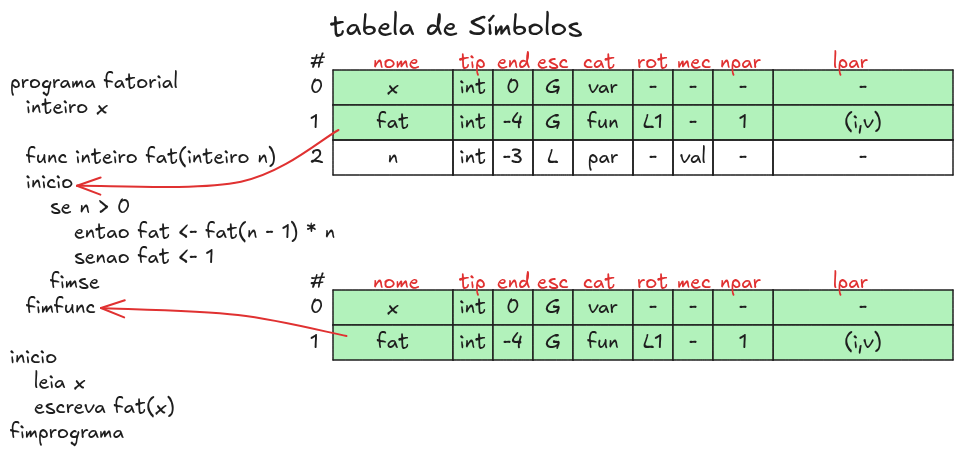
\includegraphics[width=0.9\linewidth,height=\textheight,keepaspectratio]{chapters/images/exemplo3.png}

}

\caption{\label{fig-exemplo3}Exemplo de compilação de função com
recursão}

\end{figure}%

E o resultado do código compilado para MVS é:

\begin{Shaded}
\begin{Highlighting}[]
    \KeywordTok{INPP}
    \KeywordTok{AMEM}    \DecValTok{1}
    \KeywordTok{DSVS}    \FunctionTok{L0}
\FunctionTok{L1}  \KeywordTok{ENSP}
    \KeywordTok{CRVL}\NormalTok{    {-}}\DecValTok{3}
    \KeywordTok{CRCT}    \DecValTok{0}
    \KeywordTok{CMMA}
    \KeywordTok{DSVF}    \FunctionTok{L2}
    \KeywordTok{AMEM}    \DecValTok{1}
    \KeywordTok{CRVL}\NormalTok{    {-}}\DecValTok{3}
    \KeywordTok{CRCT}    \DecValTok{1}
    \KeywordTok{SUBT}
    \KeywordTok{SVCP}
    \KeywordTok{DSVS}    \FunctionTok{L1}
    \KeywordTok{CRVL}\NormalTok{    {-}}\DecValTok{3}
    \KeywordTok{MULT}
    \KeywordTok{ARZL}\NormalTok{    {-}}\DecValTok{4}
    \KeywordTok{DSVS}    \FunctionTok{L3}
\FunctionTok{L2}  \KeywordTok{NADA}
    \KeywordTok{CRCT}    \DecValTok{1}
    \KeywordTok{ARZL}\NormalTok{    {-}}\DecValTok{4}
\FunctionTok{L3}  \KeywordTok{NADA}
    \KeywordTok{RTSP}    \DecValTok{1}
\FunctionTok{L0}  \KeywordTok{NADA}
    \KeywordTok{LEIA}
    \KeywordTok{ARZG}    \DecValTok{0}
    \KeywordTok{AMEM}    \DecValTok{1}
    \KeywordTok{CRVG}    \DecValTok{0}
    \KeywordTok{SVCP}
    \KeywordTok{DSVS}    \FunctionTok{L1}
    \KeywordTok{ESCR}
    \KeywordTok{DMEM}    \DecValTok{1}
    \KeywordTok{FIMP}
\end{Highlighting}
\end{Shaded}

O código apresentado corresponde à tradução de uma função recursiva que
calcula o fatorial de um número inteiro não negativo. A função utiliza
uma estrutura condicional para identificar o caso-base da recursão e,
quando necessário, realiza uma chamada a si própria para calcular o
fatorial do número imediatamente anterior.

A função implementa a seguinte definição matemática:

\[ f(n)= \begin{cases} 1, & \text{se } n \leq 0\\\ n \times f(n-1), & \text{se } n > 0 \end{cases} \]

A tradução pode ser dividida em três partes: inicialização do programa,
implementação da função recursiva e programa principal responsável pela
leitura do valor, chamada da função e apresentação do resultado.

\emph{Inicialização do programa}

\begin{Shaded}
\begin{Highlighting}[]
    \KeywordTok{INPP}
    \KeywordTok{AMEM}    \DecValTok{1}
    \KeywordTok{DSVS}    \FunctionTok{L0}
\end{Highlighting}
\end{Shaded}

A instrução \texttt{INPP} inicializa a execução do programa. Em seguida,
\texttt{AMEM\ 1} reserva uma posição de memória para armazenar a
variável global utilizada pelo programa principal. A instrução
\texttt{DSVS\ L0} realiza um desvio incondicional para o rótulo
\texttt{L0}, evitando que o fluxo de execução passe diretamente pelo
código da função.

O rótulo \texttt{L1}, apresentado posteriormente, identifica o ponto de
entrada da função recursiva. Dessa forma, sua execução ocorrerá somente
quando houver uma chamada.

\emph{Implementação da função recursiva}

O trecho seguinte apresenta a implementação da função responsável pelo
cálculo do fatorial:

\begin{Shaded}
\begin{Highlighting}[]
\FunctionTok{L1}  \KeywordTok{ENSP}
    \KeywordTok{CRVL}\NormalTok{    {-}}\DecValTok{3}
    \KeywordTok{CRCT}    \DecValTok{0}
    \KeywordTok{CMMA}
    \KeywordTok{DSVF}    \FunctionTok{L2}
\end{Highlighting}
\end{Shaded}

A instrução \texttt{ENSP} inicia a execução da função, preparando o
ambiente necessário para o processamento de sua chamada.

Em seguida, as instruções \texttt{CRVL\ -3} e \texttt{CRCT\ 0} recuperam
o valor do parâmetro recebido e carregam a constante zero na pilha,
respectivamente. A instrução \texttt{CMMA} realiza a comparação entre
esses valores, verificando se o parâmetro é maior que zero.

O resultado da comparação é utilizado pela instrução \texttt{DSVF\ L2},
que realiza um desvio condicional para o rótulo \texttt{L2} caso a
condição seja falsa. Portanto, quando o parâmetro for menor ou igual a
zero, a execução seguirá diretamente para o tratamento do caso-base da
recursão.

\emph{Caso recursivo}

Quando o parâmetro é maior que zero, a execução prossegue com as
seguintes instruções:

\begin{Shaded}
\begin{Highlighting}[]
    \KeywordTok{AMEM}    \DecValTok{1}
    \KeywordTok{CRVL}\NormalTok{    {-}}\DecValTok{3}
    \KeywordTok{CRCT}    \DecValTok{1}
    \KeywordTok{SUBT}
    \KeywordTok{SVCP}
    \KeywordTok{DSVS}    \FunctionTok{L1}
\end{Highlighting}
\end{Shaded}

Nesse trecho, o compilador gera o código necessário para realizar uma
nova chamada à própria função. Inicialmente, \texttt{AMEM\ 1} reserva
uma posição de memória para armazenar o resultado da chamada recursiva.

As instruções \texttt{CRVL\ -3} e \texttt{CRCT\ 1} carregam o valor do
parâmetro atual e a constante um. Em seguida, \texttt{SUBT} calcula a
diferença entre esses valores, produzindo
\textbackslash(n-1\textbackslash).

A instrução \texttt{SVCP} prepara os parâmetros para a chamada da
função, e \texttt{DSVS\ L1} transfere o fluxo de execução para o início
da própria rotina.

Dessa maneira, a função passa a executar uma nova instância de si mesma,
agora com o argumento \textbackslash(n-1\textbackslash). Esse processo
se repete até que a condição de parada seja satisfeita.

Após o retorno da chamada recursiva, a execução prossegue com:

\begin{Shaded}
\begin{Highlighting}[]
    \KeywordTok{CRVL}\NormalTok{    {-}}\DecValTok{3}
    \KeywordTok{MULT}
    \KeywordTok{ARZL}\NormalTok{    {-}}\DecValTok{4}
    \KeywordTok{DSVS}    \FunctionTok{L3}
\end{Highlighting}
\end{Shaded}

Nesse momento, o resultado da chamada recursiva está disponível na
pilha. A instrução \texttt{CRVL\ -3} recupera o valor do parâmetro da
chamada atual, enquanto \texttt{MULT} multiplica esse valor pelo
resultado obtido na chamada recursiva.

A instrução \texttt{ARZL\ -4} armazena o resultado da multiplicação na
posição de memória relativa reservada para o retorno da função.
Finalmente, \texttt{DSVS\ L3} desvia a execução para o ponto de
encerramento da rotina, evitando que o caso-base seja executado.

\emph{Caso-base da recursão}

O caso-base é implementado pelo seguinte trecho:

\begin{Shaded}
\begin{Highlighting}[]
\FunctionTok{L2}  \KeywordTok{NADA}
    \KeywordTok{CRCT}    \DecValTok{1}
    \KeywordTok{ARZL}\NormalTok{    {-}}\DecValTok{4}
\end{Highlighting}
\end{Shaded}

Quando o parâmetro recebido é menor ou igual a zero, o desvio
condicional \texttt{DSVF\ L2} direciona a execução para esse trecho.

A instrução \texttt{NADA} identifica o ponto de entrada do caso-base,
sem realizar nenhuma operação sobre a pilha. Em seguida,
\texttt{CRCT\ 1} carrega a constante um, que corresponde ao resultado do
fatorial para os valores considerados no caso-base.

A instrução \texttt{ARZL\ -4} armazena esse valor na posição de memória
destinada ao resultado da função.

Após o tratamento dos dois caminhos de execução, o fluxo converge para o
rótulo \texttt{L3}:

\begin{Shaded}
\begin{Highlighting}[]
\FunctionTok{L3}  \KeywordTok{NADA}
    \KeywordTok{RTSP}    \DecValTok{1}
\end{Highlighting}
\end{Shaded}

A instrução \texttt{NADA} marca o ponto de convergência dos caminhos de
execução. Finalmente, \texttt{RTSP\ 1} encerra a execução da função e
retorna ao ponto imediatamente posterior à chamada, disponibilizando o
resultado calculado e realizando o tratamento da estrutura de chamada,
considerando um parâmetro.

\emph{Programa principal}

Após a implementação da função, o código apresenta o programa principal,
responsável por obter o valor de entrada, realizar a chamada da função
recursiva e apresentar o resultado.

\begin{Shaded}
\begin{Highlighting}[]
\FunctionTok{L0}  \KeywordTok{NADA}
    \KeywordTok{LEIA}
    \KeywordTok{ARZG}    \DecValTok{0}
    \KeywordTok{AMEM}    \DecValTok{1}
    \KeywordTok{CRVG}    \DecValTok{0}
    \KeywordTok{SVCP}
    \KeywordTok{DSVS}    \FunctionTok{L1}
    \KeywordTok{ESCR}
    \KeywordTok{DMEM}    \DecValTok{1}
    \KeywordTok{FIMP}
\end{Highlighting}
\end{Shaded}

O rótulo \texttt{L0} identifica o início do programa principal. A
instrução \texttt{NADA} funciona como ponto de referência para o início
da execução desse trecho.

A instrução \texttt{LEIA} solicita a entrada de um valor pelo usuário.
Em seguida, \texttt{ARZG\ 0} armazena o valor informado na posição zero
da memória global, que foi previamente reservada pela instrução
\texttt{AMEM\ 1}.

Na sequência, o programa prepara a chamada da função:

\begin{itemize}
\tightlist
\item
  \texttt{AMEM\ 1}: reserva uma posição de memória para armazenar o
  resultado da função;
\item
  \texttt{CRVG\ 0}: recupera o valor armazenado na posição zero da
  memória global, que será utilizado como argumento;
\item
  \texttt{SVCP}: prepara os parâmetros para a chamada da função;
\item
  \texttt{DSVS\ L1}: transfere o fluxo de execução para o início da
  função recursiva.
\end{itemize}

Quando a função termina sua execução, a instrução \texttt{RTSP\ 1}
retorna ao programa principal, disponibilizando o resultado calculado. A
instrução \texttt{ESCR} apresenta esse resultado na saída padrão.

Finalmente, \texttt{DMEM\ 1} libera a posição de memória reservada para
o resultado da chamada, enquanto \texttt{FIMP} encerra a execução do
programa.

\emph{Exemplo de execução da função recursiva}

Para compreender o funcionamento da recursividade, considere que o
usuário informe o valor 4. Nesse caso, a função realizará as seguintes
chamadas:

Etapa 1 --- Expansão das chamadas recursivas

f(4)

4 × f(3)

f(3)

3 × f(2)

f(2)

2 × f(1)

f(1)

1 × f(0)

Caso-base

f(0) = 1

Etapa 2 --- Retorno das chamadas

\begin{longtable*}[]{|l|l|l|}
\toprule\noalign{}
Chamada & Operação & Resultado \\
\midrule\noalign{}
\endhead
\bottomrule\noalign{}
\endlastfoot
f(0) & 1 & 1 \\
\midrule
f(1) & 1 × 1 & 1 \\
\midrule
f(2) & 2 × 1 & 2 \\
\midrule
f(3) & 3 × 2 & 6 \\
\midrule
f(4) & 4 × 6 & 24 \\
\end{longtable*}

Resultado apresentado pela instrução ESCR

\[24\]

Esse exemplo permite observar aspectos importantes da tradução de
funções recursivas para a máquina virtual MVS.

Primeiramente, cada chamada recursiva cria um novo ambiente de execução,
preservando os valores dos parâmetros e as informações necessárias para
que a execução possa retornar corretamente à chamada anterior. Isso é
fundamental, pois cada instância da função possui seu próprio valor de
parâmetro e seu próprio resultado parcial.

Além disso, a utilização de endereços relativos, como \texttt{-3} e
\texttt{-4}, permite que o mesmo código da função seja executado em
diferentes níveis de recursividade, sem a necessidade de gerar uma cópia
do código para cada chamada. O mecanismo de chamadas e retornos da MVS é
responsável por manter os ambientes de execução independentes.

Por fim, observa-se que a tradução de uma função recursiva exige que o
compilador trate adequadamente a reserva de memória, a passagem de
parâmetros, o armazenamento do resultado e o retorno ao ponto de
chamada. Esses mecanismos permitem implementar funções recursivas sem
que seja necessário conhecer antecipadamente a quantidade de chamadas
que ocorrerão durante a execução do programa.

\subsection{Modificações no projeto de
compilador}\label{modificauxe7uxf5es-no-projeto-de-compilador}

A ampliação do compilador existente exige alterações coordenadas na
gramática, na análise semântica, na tabela de símbolos e na geração de
código.

No arquivo de especificação do Bison, será necessário incluir produções
para declarações de funções e procedimentos, parâmetros formais, listas
de argumentos, chamadas e comandos de retorno. As ações semânticas
deverão registrar as informações das declarações, verificar as chamadas
e emitir as instruções correspondentes.

A tabela de símbolos deverá armazenar as informações adicionais dos
subprogramas e dos seus parâmetros. A organização por escopos permitirá
distinguir variáveis globais, parâmetros e variáveis locais. Para
verificar uma chamada, o compilador deverá comparar os argumentos
efetivos com a assinatura registrada para a função ou o procedimento.

A geração de código precisará definir uma convenção de chamada. Essa
convenção deverá especificar como os argumentos são transmitidos, como o
endereço de retorno é armazenado, onde ficam as variáveis locais e como
o resultado de uma função é devolvido.

As mudanças podem ser implementadas progressivamente:

\begin{enumerate}
\def\labelenumi{\arabic{enumi}.}
\tightlist
\item
  \textbf{Declaração de procedimentos sem parâmetros:} introduzir a
  estrutura de declaração, o corpo e a chamada, além das instruções de
  transferência de controle e retorno.
\item
  \textbf{Declaração de funções:} permitir o retorno de valores e a
  utilização de chamadas em expressões.
\item
  \textbf{Parâmetros por valor:} incluir parâmetros formais e argumentos
  efetivos, com verificação de quantidade e tipos.
\item
  \textbf{Parâmetros por referência:} implementar a transmissão de
  endereços e o acesso às variáveis do chamador.
\item
  \textbf{Escopos e recursão:} organizar as tabelas de símbolos e os
  registros de ativação para permitir chamadas aninhadas e recursivas.
\end{enumerate}

Essa sequência permite validar cada recurso isoladamente antes de
combinar todos eles em programas mais complexos.

\subsection{Atividades propostas}\label{atividades-propostas}

Para consolidar os conceitos, propõe-se ampliar o compilador
desenvolvido nos capítulos anteriores, implementando as funcionalidades
na ordem apresentada.

\textbf{Atividade 1 --- Procedimentos sem parâmetros.} Estenda a
gramática para declarar um procedimento sem parâmetros e permitir sua
chamada a partir do programa principal. Gere o código necessário para
transferir a execução ao procedimento e retornar ao comando seguinte.

\textbf{Atividade 2 --- Funções com retorno inteiro.} Implemente funções
que recebam parâmetros e retornem valores inteiros. Permita que uma
chamada seja utilizada em expressões aritméticas e verifique o tipo do
resultado durante a análise semântica.

\textbf{Atividade 3 --- Verificação de argumentos.} Amplie a tabela de
símbolos para armazenar a quantidade e os tipos dos parâmetros de cada
subprograma. Detecte chamadas com quantidade incorreta de argumentos ou
com tipos incompatíveis.

\textbf{Atividade 4 --- Passagem por valor.} Implemente a transmissão
dos valores dos argumentos para os parâmetros formais. Verifique, por
meio de um programa de teste, que a alteração de um parâmetro local não
modifica a variável original do chamador.

\textbf{Atividade 5 --- Passagem por referência.} Amplie a linguagem
para permitir parâmetros por referência. Implemente a transmissão de
endereços e verifique que as modificações realizadas no subprograma são
observadas pelo chamador.

\textbf{Atividade 6 --- Variáveis locais e escopos.} Permita declarações
locais em funções e procedimentos. Garanta que identificadores locais
sejam tratados separadamente dos identificadores de outros escopos.

\textbf{Atividade 7 --- Recursão.} Implemente uma função recursiva, como
o cálculo do fatorial. Verifique se cada ativação mantém seus parâmetros
e endereço de retorno, sem interferir nas ativações anteriores.

\subsection{Considerações finais}\label{considerauxe7uxf5es-finais-2}

A inclusão de funções, procedimentos e passagem de parâmetros representa
uma evolução importante do projeto de compilador. Esses recursos ampliam
a expressividade da linguagem e exigem que o compilador controle não
apenas as construções sintáticas e os tipos, mas também a organização
dos dados e o fluxo de execução durante as chamadas.

O projeto permite integrar diversos conceitos estudados ao longo do
livro: gramáticas livres de contexto, tradução dirigida por sintaxe,
análise semântica, tabela de símbolos, geração de código e organização
da memória. Ao implementar esses recursos, o estudante passa a
compreender como abstrações presentes nas linguagens de alto nível são
traduzidas para operações executáveis por uma máquina virtual.

A implementação deve ser realizada de maneira incremental, definindo
primeiro a sintaxe e a semântica das novas construções e, em seguida,
estabelecendo a convenção de chamada e o código correspondente. Como as
instruções específicas para chamadas e retornos dependem da arquitetura
da MVS, essa etapa também pode exigir a extensão da máquina virtual
utilizada nos projetos anteriores.

Ao final, o compilador deverá ser capaz de traduzir programas
estruturados em subprogramas, verificar a consistência das declarações e
chamadas e gerar código que preserve o comportamento esperado durante a
execução. Esse resultado constitui uma base para futuras extensões, como
parâmetros opcionais, sobrecarga de funções, tipos estruturados e
mecanismos mais sofisticados de gerenciamento de memória.

Observação para a implementação: como os arquivos do projeto
apresentados anteriormente não especificam instruções da MVS para
chamada e retorno de subprogramas, o texto trata essa parte de forma
conceitual, sem atribuir à máquina instruções que ainda não foram
definidas. Antes de apresentar o código definitivo do compilador, será
necessário estabelecer a convenção de chamada e verificar se a MVS atual
oferece os mecanismos necessários ou precisa ser ampliada.

\bookmarksetup{startatroot}

\chapter{Sumário}\label{sumuxe1rio}

\bookmarksetup{startatroot}

\chapter*{Referências}\label{referuxeancias}
\addcontentsline{toc}{chapter}{Referências}

\markboth{Referências}{Referências}

\phantomsection\label{refs}
\begin{CSLReferences}{0}{1}
\bibitem[\citeproctext]{ref-hopcroft}
HOPCROFT, John E.; MOTWANI, Rajeev; ULLMAN, Jeffrey D.
\textbf{Introduction to Automata Theory, Languages, and Computation}. 3.
ed. Upper Saddle River, NJ: Pearson Addison-Wesley, 2007.

\bibitem[\citeproctext]{ref-kozen}
KOZEN, Dexter C. \textbf{Automata and Computability}. New York:
Springer, 1997.

\bibitem[\citeproctext]{ref-lewis}
LEWIS, Harry R.; PAPADIMITRIOU, Christos H. \textbf{Elementos da Teoria
da Computação}. Porto Alegre: Bookman, 2004.

\bibitem[\citeproctext]{ref-gersting}
L.GERSTING, J. \textbf{Fudamentos matemáticos para a Ciência da
Computação: um tratamento moderno de matemática discreta}. Rio de
Janeiro: LTC, 2004.

\bibitem[\citeproctext]{ref-sipser}
SIPSER, Michel. \textbf{Introdução a Teoria da Computação}. São Paulo:
Cengage Learning, 2012.

\bibitem[\citeproctext]{ref-vieira}
VIEIRA, Newton José. \textbf{Introdução aos fundamentos da computação}.
São Paulo: Pioneira Thompson Learning, 2006.

\end{CSLReferences}


\backmatter


\end{document}
